\documentclass[12pt,twoside,a4paper]{memoir}
\raggedbottom
\renewcommand{\footnoterule}{\vfill\kern -3pt \hrule width 0.4\columnwidth \kern
	2.6pt}
\usepackage{fontspec,xltxtra,xunicode}
\usepackage{imakeidx}
\indexsetup{level=\chapter*, toclevel=chapter, headers={\indexname}{\indexname}}
\usepackage{afterpage}
\usepackage{polyglossia}
\setdefaultlanguage[variant=spanish]{spanish}
\setmainlanguage[variant=spanish]{spanish}
\setotherlanguage[spelling=new,babelshorthands=true]{german}
\setotherlanguage[variant=british]{english}
\usepackage{datetime2}
\usepackage{csvsimple}
\usepackage{amsmath,amssymb}
\usepackage{unicode-math}
\setmathfont{Latin Modern Math}
\setmainfont[Ligatures=TeX,SlantedFont=*,SlantedFeatures={FakeSlant=0.2}]{CMU Serif}
\setsansfont{CMU Sans Serif}
\setmonofont{CMU Typewriter Text}
\usepackage{icomma}
\usepackage{slantsc}	
%\nouppercaseheads 
%\usepackage[toc,page]{appendix}
\usepackage{textcomp}
\usepackage{microtype}
\usepackage{gb4e}
\noautomath
%\usepackage{quotchap}
\usepackage{enumitem}
\usepackage{tikz}
\usetikzlibrary{calc,plotmarks,decorations.text,shapes,matrix,positioning,fit,backgrounds,arrows.meta,shadows,ext.positioning-plus}
\usepackage{tikz-qtree,tikz-qtree-compat}
\usepackage{nonumonpart}
\usepackage{multirow}
%\usepackage{setspace}
\usepackage{tabto}
\usepackage{nowidow}
\usepackage{url}
%\urlstyle{same}
%\def\UrlBreaks{\do\//\do-\do:}
%\usepackage[hyphenbreaks]{breakurl}
\usepackage{linegoal}
\usepackage{multicol}
\usepackage{hyphenat}
\usepackage[artemisia]{textgreek}
\usepackage{metrix}
%\setmetrixvar{symbolshift}{-0.6em}
\usepackage{scrbase}
\usepackage{listings}
%\usepackage{listingsutf8}

\usepackage{bigdelim}%
\usepackage{threeparttable}
\usepackage[labelfont=bf]{caption}
\usepackage{booktabs}

\usepackage{pgfplots}
\usepackage{pgfplotstable}
\usepackage{subcaption}
\usepackage{shapepar, varwidth}
\usepackage{multicol}
% Para Verbatim
\usepackage{fancyvrb}
%\defbibfilter{primary}{notkeyword=secondary}
%x\defbibfilter{secondary}{keyword=secondary}
\usepackage[spanish,onelanguage,plain, noend, ruled]{algorithm2e}

%\usepackage{draftwatermark}
%\SetWatermarkLightness{ 0.95 }
%\SetWatermarkText{BORRADOR}
%\SetWatermarkScale{  }


\title{Ritmo y estructura de la comedia áurea: posibilidades y límites del análisis digital automático del teatro español clásico}
\author{Fernando Sanz-Lázaro}
\makeindex[intoc]

\usepackage[edges]{forest}
%
% Bibliografía
\usepackage[tools={manuscripts,bookinother,morenames},bibstyle=apa]{biblatex-multiple-dm}
\usepackage[citestyle=apa,bibstyle=multiple-dm,backend=biber]{biblatex}
\makeatletter
\DeclareLanguageMapping{spanish}{spanish-apa}
\renewcommand*{\apablx@ifrevnameappcomma}[2]{#2}
\DefineBibliographyExtras{spanish}{%
		\let\finalandcomma=\empty
	\setcounter{smartand}{1}%
	\let\lbx@finalnamedelim=\lbx@es@smartand
	\let\lbx@finallistdelim=\lbx@es@smartand
}
\DeclareDelimFormat*{apadelim}{\addcomma\space}
\renewbibmacro*{name:delim:apa:family-given}[1]{%
	\ifnumgreater{\value{listcount}}{\value{liststart}}
	{\ifboolexpr{
			test {\ifnumless{\value{listcount}}{\value{liststop}}}
			or
			test \ifmorenames
		}
		{\printdelim{multinamedelim}}
		{\lbx@finalnamedelim{#1}}}
	{}}
\makeatother

\addbibresource{references.bib}
% Acrónimos
\usepackage{acro}
\acsetup{first-style=short}
 
% probably a good idea for the nomenclature entries:
% class `abbrev': abbreviations:
\DeclareAcronym{adso}{
	short = {ADSO},
	long  = {Análisis Distante del soneto castellano de los Siglos de Oro (\textsc{xvi} y \textsc{xvii})},
	tag = {abbrev}
}

\DeclareAcronym{afi}{
	short = {AFI\index{Alfabeto Fonético Internacional}},
	long  = {Alfabeto Fonético Internacional\index{Alfabeto Fonético Internacional}},
	tag = abbrev
}

\DeclareAcronym{ascii}{
	short = {ASCII\index{ASCII}},
	long  = {American Standard Code for Information Interchange\index{ASCII}},
	tag = abbrev
}

\DeclareAcronym{bert}{
	short = {BERT\index{BERT}},
	long  = {Bidirectional Encoder Representations from Transformers},
	tag = {abbrev}
}

\DeclareAcronym{corde}{
	short = {CORDE},
	long = {Corpus Diacrónico del Español},
	tag = abbrev,
}	

\DeclareAcronym{corpes}{
	short = {CORPES},
	long = {Corpus Español},
	tag = abbrev,
}	

\DeclareAcronym{crea}{
	short = {CREA},
	long = {Corpus de Referencia del Español Actual},
	tag = abbrev,
}

\DeclareAcronym{csv}{
	short = {CSV\index{CSV}},
	long  = {Comma Separated Values\index{CSV}},
	tag = abbrev
}

\DeclareAcronym{doc}{
	short = {DOC\index{DOC}},
	long  =  {Microsoft Word Document\index{DOC}},
	tag = abbrev
}

\DeclareAcronym{esprit}{
	short = {ESPRIT\index{ESPRIT}},
	long  = {European Strategic Programme on Research in Information Technology\index{ESPRIT}},
	tag = abbrev
}

\DeclareAcronym{fair}{
	short = {FAIR\index{FAIR}},
	long  = {Findability, accesibility, interoperability, and reusability},
	tag = {abbrev}
}

\DeclareAcronym{gnu}{
	short = {GNU\index{GNU}},
	long  = {GNU is Not Unix\index{GNU}},
	tag = abbrev
}

\DeclareAcronym{gpl}{
	long = {General Public License\index{GPL}},
	short  = {GPL\index{GPL}},
	tag = abbrev
}

\DeclareAcronym{griso}{
	short = {GRISO},
	long  = {Grupo de Investigación Siglo de Oro},
	tag = abbrev
}

\DeclareAcronym{html}{
	long = {Hyper Text Markuup Language\index{HTML}},
	short  = {HTML\index{HTML}},
	tag = abbrev
}

\DeclareAcronym{ipa}{
	short = {IPA\index{Alfabeto Fonético Internacional}},
	long  = {International Phonetic Alphabet\index{Alfabeto Fonético Internacional}},
	tag = abbrev
}

\DeclareAcronym{iso}{
	short = {ISO\index{ISO}},
	long = {International Organization for Standardization\index{ISO}},
	tag = abbrev
}

\DeclareAcronym{odf}{
	short = {ODF\index{ODF}},
	long = {Open Document Format for Office Applications\index{ODF}},
	tag = abbrev
}

\DeclareAcronym{odt}{
	short = {ODT\index{ODT}},
	long = {Open Document Text\index{ODT}},
	tag = abbrev
}

\DeclareAcronym{pdf}{
	short = {PDF\index{PDF}},
	long  = {Portable Document Format\index{PDF}},
	tag = abbrev
}

\DeclareAcronym{pln}{
	short = {PLN\index{procesamiento del lenguaje natural}},
	long  = {Procesamiento del lenguaje natural\index{procesamiento del lenguaje natural}\index{PLN|see {procesamiento del lenguaje natural}}},
	tag = abbrev
}

\DeclareAcronym{poo}{
	short = {POO\index{programación!orientada a objetos}},
	long  = {Programación orientada a objetos\index{programación!orientada a objetos}\index{POO|see {programación orientada a objetos}}},
	tag = abbrev
}

\DeclareAcronym{rae}{
	short = {RAE},
	long  = {Real Academia Española},
	tag = abbrev
}

\DeclareAcronym{regex}{
	short = {regex\index{expresión regular}},
	long  = {Regular expression\index{regex|see {expresión regular}}\index{expresión regular}},
	tag = abbrev
}

\DeclareAcronym{sampa}{
	short = {SAMPA\index{SAMPA}},
	long  = {Speech Assessment Methods Phonetic Alphabet\index{SAMPA}},
	tag = abbrev
}

\DeclareAcronym{sgml}{
	short = {SGML\index{SGML}},
	long = {Standard Generalized Markup Language\index{SGML}},
	tag = abbrev,
}

\DeclareAcronym{tei}{
	short = {TEI\index{TEI}},
	long  = {Text Encoding Initiative\index{TEI}},
	tag = {abbrev}
}

\DeclareAcronym{ved}{
	short = {VED\index{VED}},
	long = {Visually-Encoded Drama\index{VED}},
	tag = abbrev,
}

\DeclareAcronym{visos}{
	short = {VISOS},
	long  = {Viennese Siglo de Oro Studies},
	tag = abbrev
}

\DeclareAcronym{xml}{
	short = {XML\index{XML}},
	long  = {eXtended Markup Language\index{XML}},
	tag = abbrev
}

\DeclareAcronym{xmltei}{
	short = {XML-TEI\strut\index{XML-TEI}},
	long  = {eXtended Markup Language-Text Encoding Initiative\index{XML-TEI}},
	tag = abbrev
}


% Hyperlinks
\usepackage[hidelinks]{hyperref}
\usepackage{bookmark}
% Listas
\setlength{\parindent}{0in}
\nonzeroparskip
%\usepackage{tipa}
\usepackage{cleveref}
\usepackage[babel]{csquotes}

\usepackage{etoolbox}
%\usepackage{lipsum} % just for dummy text
\settypeblocksize{260mm}{160mm}{*}
\setulmarginsandblock{3.5cm}{2.5cm}{*}
\setheadfoot{\onelineskip}{2\onelineskip}
\setheaderspaces{2cm}{*}{*}


\setlrmarginsandblock{3cm}{2.5cm}{*}
\checkandfixthelayout
\OnehalfSpacing
\NewBibliographyString{organizer}
\NewBibliographyString{coordinator}
\NewBibliographyString{director}
\DefineBibliographyStrings{spanish}{%
	collaborator =	{colab\adddot},
	collaborators =	{colabs\adddot},
	director	=	{dir\adddot}
	organizer = {coord\adddot},
	organizers = {coords\adddot},
	directors	=	{dirs\adddot}
}

\makeatletter
\def\invisiblesection#1{%
	\refstepcounter{section}%
	\addcontentsline{toc}{section}{\protect\numberline{\thesection}#1}%
	\sectionmark{#1}\phantom{}
	\protected@edef\@currentlabelname{#1} % Set correct name
}
\makeatother

\renewbibmacro*{apaeditorstrg}[1]{%
	\iffieldundef{#1type}
	{\ifthenelse{\value{#1}>1\OR\ifandothers{#1}}
		{\bibcpstring{editors}}
		{\bibcpstring{editor}}}
	{\ifthenelse{\value{#1}>1\OR\ifandothers{#1}}
		{\ifbibstring{type\thefield{#1type}s}
			{\bibcpstring{type\thefield{#1type}s}}
			{\bibcpstring{\thefield{#1type}s}}}
		{\ifbibstring{type\thefield{#1type}}
			{\bibcpstring{type\thefield{#1type}}}
			{\bibcpstring{\thefield{#1type}}}}}}

\newfontfamily\myregularfont{CMU Serif}
\newfontfamily\DVS{DejaVu Sans}
\newfontfamily\Arial{Arial}
\newfontfamily\ipafont{CMU Serif}
\newfontfamily\sans{CMU Sans Serif}
\newcommand{\ipa}[1]{{\ipafont\textipa{#1}}}

\newcommand\posscite[1]{\citeauthor{#1}'s (\citeyear{#1})}
\newcommand{\iindex}[1]{#1\index{#1}} 
\tikzset{every tree node/.style={font=\itshape}}
\tikzset{
	module/.style={%
		draw, rounded corners,
		minimum width=#1,
		minimum height=7mm,
		align=center
	},
	module/.default=2cm,
	>=LaTeX
}

\tikzset{
	datos/.style={%
		draw,
		minimum width=#1,
		minimum height=7mm,
		tape,
		tape bend top=none,
		fill=white,
		double copy shadow,
		minimum height=1.5cm,
		align=center
	},
	datos/.default=2cm,
	>=LaTeX
}

\tikzset{
	dato/.style={%
		draw,
		minimum width=#1,
		minimum height=7mm,
		tape,
		tape bend top=none,
		fill=white,
		align=center
	},
	dato/.default=2cm,
	>=LaTeX
}

%\colorlet{myblue}{blue!50!black}
\colorlet{myblue}{black!60}
\colorlet{myred}{black!60}
\colorlet{myyellow}{yellow!90!black!60}
%\colorlet{myred}{red!80!black!60}
\pgfdeclareverticalshading{rainbow}{100bp}{
	color(0bp)=(red); color(25bp)=(red); color(35bp)=(yellow);
	color(45bp)=(green); color(55bp)=(cyan); color(65bp)=(blue);
	color(75bp)=(violet); color(100bp)=(violet)
}
\newcaptionname{spanish}{\lstlistingname}{Listado}
\def\dollar{\$}
\lstset{
	basicstyle=\footnotesize\ttfamily,  %Looks much better.
	%columns=flexible, %Without this you get fixed-width fonts, which look bad.
	breaklines=true,   %End-of-line wrap - you really want this, usually.
	language=Python, 
	texcl=true,
	extendedchars=true,
	columns=fullflexible,
	keepspaces=true
	%basewidth=0.4em,
	%inputencoding=utf8
	upquote=true,
	numbers=left,
	escapeinside={*@}{@*)},
	xleftmargin=5ex,
	%xrightmargin=5ex
	showstringspaces=false,
	breakatwhitespace   = true,
	prebreak= \space,
	postbreak   = \space,
	literate={4>}{\$}1
}
\makeatletter
\lst@InputCatcodes
\def\lst@DefEC{%
	\lst@CCECUse \lst@ProcessLetter
	^^80^^81^^82^^83^^84^^85^^86^^87^^88^^89^^8a^^8b^^8c^^8d^^8e^^8f%
	^^90^^91^^92^^93^^94^^95^^96^^97^^98^^99^^9a^^9b^^9c^^9d^^9e^^9f%
	^^a0^^a1^^a2^^a3^^a4^^a5^^a6^^a7^^a8^^a9^^aa^^ab^^ac^^ad^^ae^^af%
	^^b0^^b1^^b2^^b3^^b4^^b5^^b6^^b7^^b8^^b9^^ba^^bb^^bc^^bd^^be^^bf%
	^^c0^^c1^^c2^^c3^^c4^^c5^^c6^^c7^^c8^^c9^^ca^^cb^^cc^^cd^^ce^^cf%
	^^d0^^d1^^d2^^d3^^d4^^d5^^d6^^d7^^d8^^d9^^da^^db^^dc^^dd^^de^^df%
	^^e0^^e1^^e2^^e3^^e4^^e5^^e6^^e7^^e8^^e9^^ea^^eb^^ec^^ed^^ee^^ef%
	^^f0^^f1^^f2^^f3^^f4^^f5^^f6^^f7^^f8^^f9^^fa^^fb^^fc^^fd^^fe^^ff%
	^^^^20ac^^^^0153^^^^0152^^^^2014^^^^2013^^^^2026^^^^2018^^^^2019^^^^03b8^^^^02a7^^^^019d^^^^0272%
	^^^^20a7^^^^2190^^^^2191^^^^2192^^^^2193^^^^2206^^^^2207^^^^220a^^^^028e^^^^027e^^^^02b0^^^^029d%
	^^^^2218^^^^2228^^^^2229^^^^222a^^^^2235^^^^223c^^^^2260^^^^2261^^^^03b2^^^^0263^^^^0115^^^^0103%
	^^^^2262^^^^2264^^^^2265^^^^2282^^^^2283^^^^2296^^^^22a2^^^^22a3^^^^0271^^^^014b^^^^03c7^^^^014f%
	^^^^22a4^^^^22a5^^^^22c4^^^^2308^^^^230a^^^^2336^^^^2337^^^^2339^^^^1ebd^^^^0129^^^^0168^^^^0169%
	^^^^233b^^^^233d^^^^233f^^^^2340^^^^2342^^^^2347^^^^2348^^^^2349^^^^fb01^^^^fb02 %
	^^^^2b7e %
	^^^^234b^^^^234e^^^^2350^^^^2352^^^^2355^^^^2357^^^^2359^^^^235d%
	^^^^235e^^^^235f^^^^2361^^^^2362^^^^2363^^^^2364^^^^2365^^^^2368^^^^0283%
	^^^^236a^^^^236b^^^^236c^^^^2371^^^^2372^^^^2373^^^^2374^^^^2375^^^^02cc^^^^02c8%
	^^^^2377^^^^2378^^^^237a^^^^2395^^^^25af^^^^25ca^^^^25cb^^^^201c^^^^201d%
	^^00}
\lst@RestoreCatcodes
\makeatother


\renewcommand{\chaptermark}[1]{\markboth{\textsc{#1}}{}}

\renewcommand{\chaptermark}[1]{\markboth{\textsc{\ifnum \c@secnumdepth >\m@ne
			\if@mainmatter
			\@chapapp %\thechapter.\
			\fi \fi #1}}{}}
\def\sectionmark#1{\markright{%\thesection.\
		#1}}
\def\chaptermark#1{\markleft{%\thesection.\
		#1}}
\setlength\headheight{16pt}

\newcommand{\unchapter}[1]{%
	\begingroup
	\let\@makechapterhead\@gobble % make \@makechapterhead do nothing
	\chapter{#1}
	\endgroup
}


\AtBeginEnvironment{algorithm}{\DontPrintSemicolon\SetAlgoNoLine\setlength{\algomargin}{1cm}}
\SetKw{nadadenada}{\strut}
\SetKw{acabacon}{acaba~con}
\SetKw{booleano}{booleano}
\SetKw{cadena}{cadena de caracteres}
\SetKw{diccionario}{diccionario}
\SetKw{set}{conjunto}
\SetKw{empiezacon}{empieza~con}
\SetKw{entero}{entero}
\SetKw{Fes}{es}
\SetKw{is}{es}
\SetKw{lista}{lista}
\SetKw{not}{no}
\SetKw{of}{de}
\SetKw{False}{Falso}
\SetKw{True}{Verdadero}
\SetKw{SiguienteIt}{SiguienteIteración}
\SetKw{Fin}{InterrumpeIteración}

\SetKwIF{If}{ElseIf}{Else}{si}{entonces}{si no, si}{si no}{fin si}

\SetKwProg{Fsubrutina}{Subrutina}{:}{}
\SetKwProg{Ffuncion}{Función}{:}{}
\SetKwProg{Fclase}{Clase}{:}{}
\SetKwProg{Fmetodo}{Método}{:}{}

\SetKwFunction{EnEscena}{EnEscena}
\SetKwFunction{ordenamayoramenor}{DeMayorAMenor}
\SetKwFunction{BuscaAsonantes}{BuscaAsonantes}
\SetKwFunction{flatten}{PalabrasASílabas}
\SetKwFunction{ResuelveLargos}{ResuelveLargo}
\SetKwFunction{EncuentraEpentesis}{EncuentraEpéntesis}
\SetKwFunction{QuitaEpentesis}{QuitaEpéntesis}
\SetKwFunction{PreferenciaDieresis}{PreferenciaDiéresis}
\SetKwFunction{EncuentraDieresis}{EncuentraDiéresis}
\SetKwFunction{AplicaDieresis}{AplicaDiéresis}
\SetKwFunction{AjustaSilabas}{AjustaSílabas}
\SetKwFunction{Sinalefas}{Sinalefas}
\SetKwFunction{AjustaPosicion}{AjustaPosicion}
\SetKwFunction{EncuentraNucleos}{EncuentraNúcleos}
\SetKwFunction{MarcaRitmo}{MarcaRitmo}
\SetKwFunction{nsilabas}{sílabas}
\SetKwFunction{ActualizaM}{ActualizaMetros}
\SetKwFunction{ActualizaT}{ActualizaTabla}
\SetKwFunction{AjustaEsperadas}{AjustaEsperadas}
\SetKwFunction{AjustaMetro}{AjustaMetro}
\SetKwFunction{AplicaSinalefas}{AplicaSinalefas}
\SetKwFunction{Fanade}{AñadeElemento}
\SetKwFunction{AnadeEpentesis}{AñadeEpéntesis}
\SetKwFunction{Valores}{Características}
\SetKwFunction{Farbol}{CompletaÁrbol}
\SetKwFunction{Correccion}{Corrección}
\SetKwFunction{escande}{Escande}
\SetKwFunction{CreaXML}{CreaXML}
\SetKwFunction{Vocales}{CuentaVocales}
\SetKwFunction{diptonga}{Diptonga}
\SetKwFunction{Per}{Perceptibility}
\SetKwFunction{DivideVariables}{DivideVariables}
\SetKwFunction{FSub}{DivideVariables}
\SetKwFunction{EncuentraSinalefas}{EncuentraSinalefas}
\SetKwFunction{EncuentraNucleos}{EncuentraNúcleos}
\SetKwFunction{EncuentraRitmo}{EncuentraRitmo}
\SetKwFunction{EncuentraRima}{EncuentraRima}
\SetKwFunction{FindPS}{EncuentraAcento}
\SetKwFunction{Estrofas}{Estrofas}
\SetKwFunction{Fautor}{EvalúaAutor}
\SetKwFunction{Fdramatis}{EvalúaElenco}
\SetKwFunction{Fdate}{EvalúaFecha}
\SetKwFunction{Flinea}{EvalúaLínea}
\SetKwFunction{EncuentraDiptongo}{EncuentraDiptongo}
\SetKwFunction{correcto}{EsCorrecto}
\SetKwFunction{AplanaLista}{AplanaLista}
\SetKwFunction{Tabla}{Tabla}
\SetKwFunction{AsignaEsquema}{AsignaEsquema}
\SetKwFunction{SetFeats}{FijaRasgos}
\SetKwFunction{Frase}{Frase}
\SetKwFunction{guardaac}{GuardaAcotación}
\SetKwFunction{guardaverso}{GuardaVerso}
\SetKwFunction{Importar}{Importar}
\SetKwFunction{inicializa}{inicializa}
\SetKwFunction{Facotacion}{IntroduceAcotación}
\SetKwFunction{Limpia}{Limpia}
\SetKwFunction{BuscaEstrofa}{BuscaEstrofa}
\SetKwFunction{limpia}{Limpia}
\SetKwFunction{fixline}{LimpiaLínea}
\SetKwFunction{MetroVerso}{MetroVerso}
\SetKwFunction{Minuscula}{Minúscula}
\SetKwFunction{PLN}{PLN}
\SetKwFunction{PreferenciaSinalefa}{PreferenciaSinalefa}
\SetKwFunction{Facto}{NuevoActo}
\SetKwFunction{Fparlamento}{NuevoParlamento}
\SetKwFunction{Valores}{Palabra}
\SetKwFunction{AnadirLinea}{AñadirLínea}
\SetKwFunction{QuitaCifras}{QuitaCifras}
\SetKwFunction{pl}{PrimeraLetra}
\SetKwFunction{preprocess}{Preprocesa}
\SetKwFunction{pl}{PrimeraLetra}
\SetKwFunction{ignora}{Pasa}
\SetKwFunction{rtag}{BuscaEtiqueta}
\SetKwFunction{rtext}{BuscaTexto}
\SetKwFunction{Reordena}{Reordena}
\SetKwFunction{sustF}{SustituciónFonética}
\SetKwFunction{Sustituye}{Sustituye}
\SetKwFunction{erre}{SustituyeR}
\SetKwFunction{tamano}{Tamaño}
\SetKwFunction{Transcripcion}{Transcripción}
\SetKwFunction{FNL}{TranscripciónFonológica}
\SetKwFunction{FNT}{TranscripciónFonética}  
\SetKwFunction{SAMPA}{TransliteraciónSAMPA}
\SetKwFunction{silabacion}{Silabación}
\SetKwFunction{ultima}{ÚltimaLetra}
\SetKwFunction{une}{Une}
\SetKwFunction{UneLista}{UneLista}
\SetKwFunction{Verso}{Verso}
\SetKwFunction{CorrigeP}{CorrigeOrtotipografía}
\SetKwFunction{Valoresp}{Valores}
\SetKwFunction{CompruebaHemistiquios}{CompruebaHemistiquios}
\SetKwFunction{AsignaSexo}{AsignaSexo}
\SetKwFunction{Romances}{Romances}
\SetKwData{rtag}{rtag}
\SetKwData{rtext}{rtext}
\SetKwData{etiqueta}{etiqueta}
	\SetKwData{nombres}{nombres}
\SetKwData{nombre}{nombre}
\SetKwData{titulo}{Título}
\SetKwData{genero}{Género}
\SetKwData{subgenero}{Subgénero}
\SetKwData{subtitulo}{Subtítulo}
\SetKwData{sexo}{sexo}
\SetKwData{s}{s}
\SetKwData{est}{est}
\SetKwData{edicion}{edición}
\SetKwData{fecha}{fecha}
\SetKwData{versos}{versos}
\SetKwData{acento}{acento}
\SetKwData{edition}{edición}
\SetKwData{acentos}{acentos}
\SetKwData{subg}{subg.}
\SetKwData{acto}{acto}
\SetKwData{actos}{actos}
\SetKwData{alos}{alófonos}
\SetKwData{amb}{ambi}
\SetKwData{ant}{anterior}
\SetKwData{arbol}{árbol}
\SetKwData{ataqueAdmisible}{ataqueAdmisible}
\SetKwData{aso}{ason}
\SetKwData{asson}{asonancia}
\SetKwData{atonas}{átonas}
\SetKwData{ataqueIndivisible}{ataqueIndivisible}
\SetKwData{cabecera}{cabecera}
\SetKwData{autor}{autor}
\SetKwData{genre}{género}
\SetKwData{caracter}{carácter}      
\SetKwData{pos}{categoría}
\SetKwData{stressedpos}{categoría_tónicaa}
\SetKwData{cerradas}{cerradas}
\SetKwData{cerrados}{cerrados}
\SetKwData{abiertos}{abiertos}
\SetKwData{codaIndivisible}{codaIndivisible}
\SetKwData{conf}{configuraciónPLN}
\SetKwData{rim}{cons}
\SetKwData{conss}{consonancia}
\SetKwData{consonantes}{consonantes}
\SetKwData{cuerpo}{cuerpo}
\SetKwData{cuenta}{n}
\SetKwData{debiles}{débiles}
\SetKwData{deletreo}{deletreos}
\SetKwData{dep}{dep}
\SetKwData{diacriticos}{diacríticos}
\SetKwData{dígrafos}{dígrafos}
\SetKwData{dipt}{diptongo}
\SetKwData{dipts}{diptongos}
\SetKwData{encontradas}{encontradas}
\SetKwData{esperadas}{esperadas}
\SetKwData{fecha}{fecha}
\SetKwData{fila}{fila}
\SetKwData{phon}{fonemas}
\SetKwData{fuertes}{fuertes}
\SetKwData{i}{i}
\SetKwData{flexiones}{flexiones}
\SetKwData{fonetica}{fonética}
\SetKwData{fonologia}{fonología}
\SetKwData{i}{i}
\SetKwData{grandtotal}{escansión}
\SetKwData{letras}{letras}
\SetKwData{linea}{línea}
\SetKwData{lineas}{líneas}
\SetKwData{media}{med}
\SetKwData{metros}{metros}
\SetKwData{variables}{metadatos}
\SetKwData{variable}{variable}
\SetKwData{musical}{musical}
\SetKwData{nuclei}{núcl}
\SetKwData{p}{pers}
\SetKwData{word}{palabra}
\SetKwData{vocalicos}{vocálicos}
\SetKwData{joint}{unión}
\SetKwData{pal}{pal}
\SetKwData{silA}{silA}
\SetKwData{silB}{silB}
\SetKwData{palA}{palA}
\SetKwData{palB}{palB}
\SetKwData{posiciones}{posiciones}
\SetKwData{words}{palabras}
\SetKwData{palabras}{palabras}
\SetKwData{parlamento}{parlamento}
\SetKwData{perceptibilidad}{perceptibilidad}
\SetKwData{personaje}{personaje}
\SetKwData{pln}{pln}
\SetKwData{posicion}{posición}
\SetKwData{preliminares}{preliminares}
\SetKwData{Vari}{posición}
\SetKwData{feats}{rasgos}
\SetKwData{recuento}{recuento}
\SetKwData{reordenada}{reordenada}
\SetKwData{resto}{resto}
\SetKwData{rhy}{ritm}
\SetKwData{sampa}{sampa}
\SetKwData{semivocales}{semivocales}
\SetKwData{silpal}{sílabas\_palabra}
\SetKwData{siltext}{sílabas\_texto}
\SetKwData{simbolos}{símbolos}
\SetKwData{silabi}{silabación}
\SetKwData{slb}{sílaba}
\SetKwData{slbs}{sílabas}
\SetKwData{sospechosos}{sospechosos\_habituales}
\SetKwData{syl}{síla}
\SetKwData{symbols}{símbolos}
\SetKwData{tabla}{tabla}
\SetKwData{texto}{texto}
\SetKwData{tonicas}{categorías\_tónicas}
\SetKwData{ton}{tónica}
\SetKwData{tton}{tón}
\SetKwData{tons}{tónicas}
\SetKwData{trans}{transliteración}
\SetKwData{transcripcion}{transcripción}
\SetKwData{trapecio}{trapecio}
\SetKwData{unidades}{unidades}
\SetKwData{unidad}{unidad}
\SetKwData{V}{V}
\SetKwData{v}{v}
\SetKwData{paux}{paux}
\SetKwData{valor}{n}
\SetKwData{n}{n}
\SetKwData{vedtext}{vedtext}
\SetKwData{verso}{verso}
\SetKwData{fixedverse}{versolisto}
\SetKwData{vocales}{vocales}

\SetKwData{fuera}{fuera}
\SetKwData{rimas}{rimas}
\SetKwData{flag}{señal}
\SetKwData{mtrs}{mtrs}
\SetKwData{union}{unión}
\SetKwData{anterior}{anterior}
\SetKwData{anterior}{anterior}
\SetKwData{siguiente}{siguiente}
\SetKwData{sinalefas}{sinalefas}
\SetKwData{estimacion}{estimación}
\SetKwData{ambiguedad}{ambigüedad}
\SetKwData{silabas}{sílabas}
\SetKwData{silaba}{sílaba}
\SetKwData{nucleo}{núcleo}
\SetKwData{ritmo}{ritmo}
\SetKwData{asonancia}{asonancia}
\SetKwData{cuenta}{cuenta}
\SetKwData{nucleos}{núcleos}
\SetKwData{rima}{rima}
\SetKwData{patron}{patrón}
\SetKwData{comunes}{comunes}
\SetKwData{slbs}{slbs}
\SetKwData{perc}{perc}
\SetKwData{nversos}{nversos}
\SetKwData{snlf}{snlf}
\SetKwData{exp}{exp}
\SetKwData{s}{s}
\SetKwData{position}{posición}
\SetKwData{preferencia}{preferencia}
\SetKwData{coda}{coda}
\SetKwData{ataque}{ataque}
\SetKwData{sC}{C}
\SetKwData{sV}{V}
\SetKwData{Vf}{V\textsubscript{F}}
\SetKwData{val}{val}
\SetKwData{offset}{desplazamiento}
\SetKwData{desplazamiento}{desplazamiento}
\SetKwData{distancia}{distancia}
\SetKwData{voc}{voc}
\SetKwData{diptongo}{diptongo}
\SetKwData{i}{i}
\SetKwData{idx}{idx}
\SetKwData{nulo}{nulo}
\SetKwData{correccion}{corrección}
\SetKwData{metro}{metro}
\SetKwData{potenciales}{potenciales}
\SetKwData{cuenta}{cuenta}
\SetKwData{diptongos}{diptongos}
\SetKwData{triptongos}{triptongos}
\SetKwData{palsil}{palsil}
\SetKwData{idx}{idx}
\SetKwData{semivocal}{semivocal}
\SetKwData{semiconsonante}{semiconsonante}
\SetKwData{parteuno}{parte1}
\SetKwData{partedos}{parte2}
\SetKwData{hiato}{hiato}
\SetKwData{dipt}{dipt}
\SetKwData{a}{a}
\SetKwData{N}{N}
\SetKwData{c}{c}
\SetKwData{orig}{origen}
\SetKwData{guardar}{guardar\_línea}
\SetKwData{epen}{epéntesis}
\SetKwData{elemento}{elemento}
\SetKwData{abiertas}{abiertas}
\SetKwData{slbs}{slbs}
\SetKwData{sllbls}{slbs}
\SetKwData{tonica}{tónica}
\SetKwData{sinalefasp}{sinalefasp}
\SetKwData{hiatosp}{diéresisp}
\SetKwData{dieresis}{diéresis}
\SetKwData{hemistiquio}{hemistiquio}
\SetKwData{estrofas}{estrofas}
\SetKwData{estrofa}{estrofa}
\SetKwData{consonancia}{consonancia}
\SetKwData{esdrujula}{esdrújula}
\SetKwData{vocoides}{vocoides}
\SetKwData{nparlamento}{parlamento\textsubscript{n}}
\SetKwData{nacotacion}{acotación\textsubscript{n}}
\SetKwData{segmento}{segmento}
\SetKwData{obra}{obra}
\SetKwData{resultado}{resultado}
\SetKwData{aquelindo}{aquelindo}
\SetKwData{listA}{lista}
\SetKwData{exceso}{exceso}
\SetKwData{resultado}{resultado}

\pgfplotsset{compat = newest}
\newcounter{para} \setcounter{para}{0}
\newcommand{\newpara}{%
	\refstepcounter{para}%
	\noindent\llap{\thepaescuelar. }\quad}
\newcommand{\oldpara}[1]{%
	\noindent\llap{\ref{#1}. }\quad}

\def\triangledownshape{%
	{0}%
	{0}b{0}\\%
	{0}t{-10}{20}\\%
	%{8.66}t{-5}{10}\\%
	{17.32}e{0}%
}
\def\triangledownpar#1{\Shapepar\triangledownshape #1\unskip\ {\fontspec{Junicode}}\par}
\newcommand{\poetics}[1]{Arist. \emph{Poet.},\@ #1\nocite{aristoteles2010}\mancite}
\newcommand{\aesthetics}[1]{Hegel \emph{Aesthetics III},\@ #1\nocite{hegel2016}\mancite}
\newcommand{\ars}[1]{Hor. \emph{Ars},\@ #1\nocite{horacio1986}\mancite}

\newcommand{\politeia}[1]{Plat. \emph{Rep.},\@ #1\nocite{platon2011}\mancite}


\clubpenalty=9996
\widowpenalty=9999
\brokenpenalty=4991
\predisplaypenalty=10000
\postdisplaypenalty=1549
\displaywidowpenalty=1602

% etoolbox
\newbool{specialtoc}

\renewcommand{\cftchapterfont}{%
	\ifbool{specialtoc}{%
		\itshape
	}{%
		\bfseries
	}%
}

\renewcommand{\cftchapterpagefont}{%
	\ifbool{specialtoc}{%
		\itshape
	}{%
		\bfseries
	}%
}


%\makeatletter
%\newcommand{\fonttitle}{\chaptitlefont}
%\makechapterstyle{mystyle}{%
%	\def\chapterheadstart{\vspace*{\beforechapskip}}
%	\def\printchaptername{}
%	\def\printchapternum{}
%	\def\printchapternonum{}
%	\def\printchaptertitle##1{%
%		\fonttitle \if@mainmatter \thechapter.\space\fi ##1}
%	\def\afterchaptertitle{\par\nobreak\vskip \afterchapskip}
%}
%\makeatother

\setlength{\cftbeforepartskip}{2.5ex}
\setlength{\cftpartnumwidth}{3em}
\setlength{\cftbeforechapterskip}{0.5ex}
\setlength{\epigraphwidth}{200pt}
\epigraphposition{flushleft}
\epigraphfontsize{\footnotesize}
\setlength{\epigraphrule}{0pt}

\newenvironment{changemargin}[3]{%
	\begin{list}{}{%
			\setlength{\leftmargin}{#1}%
			\setlength{\rightmargin}{#2}%
			\setlength{\topmargin}{#3}%
		}%
		\item[]}
	{\end{list}}
\raggedbottom


\newcounter{excurso}
\setcounter{excurso}{1}
\newcommand*\rot{\rotatebox{90}}
%\makeatletter
%\DefineBibliographyExtras{spanish}{%
%	\protected\def\mkbibmascord#1{\stripzeros{#1}.\textsuperscript{o}}%
%	\protected\def\mkbibfemord#1{\stripzeros{#1}.\textsuperscript{a}}
%	\setcounter{smartand}{0}%
%	\renewbibmacro*{name:delim:apa:family-given}[1]{%
%		\ifnumgreater{\value{listcount}}{\value{liststart}}
%		{\ifboolexpr{
%				test {\ifnumless{\value{listcount}}{\value{liststop}}}
%				or
%				test \ifmorenames
%			}
%			{\printdelim{multinamedelim}}
%			{\lbx@finallistdelim{#1}}}
%		{}}%
%}
%\makeatother

%\DefineBibliographyStrings{spanish}{%
%	andothers = {et al\adddot}
%}

\usepackage{xcolor,fix-cm}
\definecolor{numbercolor}{gray}{0.7}
\newif\ifchapternonum
\makechapterstyle{jenor}{
	\setlength{\beforechapskip}{50pt}
	\setlength{\midchapskip}{40pt}
	\setlength{\afterchapskip}{60pt}
	\renewcommand\chapterheadstart{\vspace*{\beforechapskip}}
	\newif\ifchapternonum
	\renewcommand\printchaptername{}
	\renewcommand\printchapternum{}
	\renewcommand\printchapternonum{\chapternonumtrue}
	\renewcommand\chaptitlefont{\myregularfont
	%\bfseries
	%\fontfamily{pbk}
	\fontseries{b}\fontshape{n}%
		%\fontseries{db}%
		%\fontshape{n}
		\fontsize{30}{36}
		%\fontsize{25}{35}
		\selectfont
		\raggedleft}
	\renewcommand\chapnumfont{%\normalfont
		\myregularfont
	%\fontfamily{pbk}
	\fontseries{bx}\fontshape{n}%
	\fontsize{1in}{0in}
	\selectfont
	\color{numbercolor}
	}
\renewcommand\printchaptertitle[1]{%
\noindent%
\ifchapternonum%
\begin{tabularx}{\textwidth}{X}%
{\parbox[b]{\linewidth}{\chaptitlefont ##1}%
\vphantom{\raisebox{-15pt}{\chapnumfont 1}}}
\end{tabularx}%
\else
\begin{tabularx}{\textwidth}{Xl}
{\parbox[b]{\linewidth}{\chaptitlefont ##1}}
& \raisebox{-15pt}{\chapnumfont \thechapter}%
\end{tabularx}%
\fi
\par\vskip2mm\hrule
}
}
\chapterstyle{jenor}

\usepackage{chngcntr}
\counterwithout{footnote}{chapter}
\OnehalfSpacing

\makepagestyle{toc}
\makeoddhead{toc}{\textit{Índice general}}{}{\thepage}
\makeevenhead{toc}{\thepage}{}{\textsc{Índice general}}
\renewcommand{\chaptermark}[1]{\markboth{%\thechapter.
		\textsc{#1}}{}}
		\def\sectionmark#1{\markright{#1}}
\makepagestyle{mystyle}
	\makeoddfoot{mystyle}{}{}{}
	\makeevenfoot{mystyle}{}{}{}
	\makeoddhead{mystyle}{\itshape\rightmark}{}{\thepage}
	\makeevenhead{mystyle}{\thepage}{}{\scshape\leftmark}
\begin{document}
	\begin{sloppypar}
    	\thispagestyle{empty}\newdimen\origiwspc%
\newdimen\origiwstr%
\origiwspc=\fontdimen2\font% original inter word space
\origiwstr=\fontdimen3\font% original inter word stretch

\begin{changemargin}{-13mm}{-8mm}{-30mm}
	\vspace*{-20.1mm}\begin{flushright}
		
\includegraphics{images/university.png}
	\end{flushright}
	
	\strut\\[8.5mm]
	\begin{center}
		{\textbf{\MakeUppercase{\huge\Arial Dissertation / Doctoral Thesis}}} \\[16.2mm]\strut
		{\normalsize\Arial{}Titel der Dissertation / Title of the Doctoral Thesis}\\[-0.9mm]				
		{\Large\Arial „Ritmo y estructura de la comedia áurea:\\posibilidades y límites del análisis digital automático del teatro español clásico“}\\[11.7mm]
		{\normalsize\Arial{}verfasst von / submitted by} \\[1.5mm]
		{\large\Arial{}Lic. Mag. Fernando Sanz-Lázaro} \\[24.2mm]
		{\normalsize\Arial angestrebter akademischer Grad / in partial fulfilment of the requirements for the degree of} \\
		\large{\Arial{}Doktor der Philosophie (Dr.phil.)}
	\end{center}\strut\\[1mm] \strut
	\begin{flushleft}
		\normalsize{\Arial{}Wien, 2023 / Vienna 2023} \\[9mm]
		\SingleSpacing
		\begin{tabular}{@{}ll}
			\small \parbox[t]{90mm}{\Arial{}Studienkennzahl lt.\ Studienblatt / \\
				degree programme code as it appears on the student\\
				record sheet:}
			&\strut \hspace{1cm}
			{\Arial\small A 792 236} \\[11mm]
			\small \parbox[t]{90mm}{\Arial{}Dissertationsgebiet  lt. Studienblatt / \\
				field of study as it appears on the student record sheet:}
			&\strut \hspace{1cm}
			{\Arial\small Romanistik / Romance Studies} \\[11mm]
			\small \parbox[t]{90mm}{\Arial{}Betreut von / Supervisor:}
			&\strut \hspace{1cm}
			{\Arial\small PD Mag. Dr. Wolfram Aichinger}
		\end{tabular}
	\end{flushleft}\vfill
	\strut
\end{changemargin}
\fontdimen2\font=\origiwspc% (original) inter word space
\fontdimen3\font=\origiwstr% (original) inter word stretch
\newpage
\thispagestyle{empty}
\begin{center}
	\fbox{\begin{minipage}{\linewidth}
			Esta tesis ha sido amparada por los proyectos de investigación \textit{El Calderón Cómico} (\href{https://pf.fwf.ac.at/en/research-in-practice/project-finder/37881}{FWF P 29115}) e \textit{Interpretation of Childbirth in Early Modern Spain} (\href{https://pf.fwf.ac.at/en/research-in-practice/project-finder/46258}{FWF  P 32263-G30}), dirigidos por el Dr. Wolfram Aichinger, y \textit{Sound and Meaning in Spanish Golden Age Literature} (\href{https://pf.fwf.ac.at/en/research-in-practice/project-finder/46968}{FWF P 32563}), dirigido por el Dr. Simon Kroll.
	\end{minipage}}
	\strut\vspace{60ex}
	
	\strut
	\begin{small}
	\begin{minipage}{\linewidth}
		Este trabajo se compuso con \XeLaTeX{} usando los tipos de letra CMU Serif y {\footnotesize\DVS{}DejaVu Sans} para el cuerpo del texto,  \texttt{CMU Typewriter} para los listados de código fuente y $Latin\ Modern\ Math$ para las fórmulas, todos bajo licencia libre; la portada incluye el tipo de letra comercial {\small\Arial{}Arial} de acuerdo con las directrices de la Universidad.
		\end{minipage}
	\vfill
		\textcopyright{} 2023 Fernando Sanz-Lázaro
		
		Bajo licencia Creative Commons Attribution 4.0 International (CC BY 4.0)\\
		
		Puede encontrar los términos de la licencia en:\\ \url{https://creativecommons.org/licenses/by/4.0/legalcode.es}
		
		
\includegraphics{images/by.png}
		
		Impreso en Viena
	\end{small}\end{center}\newpage
	
		\frontmatter
			\setlength{\cftbeforechapterskip}{0pt}
			\pagestyle{empty}
			%\input{porta}\cleardoublepage
			\thispagestyle{empty}
\strut
\vspace{20ex}
\begin{center}A Carlotta y Mateo\end{center}
\cleardoublepage

			%\input{frase}
			\pagestyle{mystyle}
			%\input{prefacio}
			\chapter*{Agradecimientos}\markboth{Agradecimientos}{Agradecimientos}

Esta tesis ha sido posible gracias al concurso de un sinnúmero de personas, que, lo sepan o no, han puesto su granito de arena —paladas, alguno—. Sirvan estas líneas al menos como un mínimo reconocimiento a todos ellos, ya que jamás podré pagarles como verdaderamente merecen. 

Para comenzar, doy las gracias a Wolfram Aichinger, mi director de tesis, amigo y maestro, por no dejarme perder de vista lo que de verdad importa, empezando por el mismo título del trabajo y acabando con aquel curso de literatura que impartió durante el primer semestre de 2014 —y mío en la Universidad de Viena— en el Auditorio A de este viejo hospital general, donde entendí hacia dónde ir.

Vaya un agradecimiento muy especial para Simon Kroll por acogerme en su equipo, motivar esta disertación y tomarse un tiempo impagable en revisar el manuscrito con la minuciosidad del editor crítico que es, pero también por todo lo que he aprendido junto a él y por estar siempre alerta para señalar nuevos caminos por explorar.
 
Gracias a  Álvaro Cuéllar, por el torbellino de ideas que ha traído a Viena consigo, por redescubrir \textit{La francesa Laura} y porque, en el breve tiempo que hemos trabajado juntos, ha inspirado no pocas cosas y contribuido a mejorar muchas otras, incluyendo su lectura crítica del manuscrito. Hago una acotación aquí —\textit{pun intended}— para dar también las gracias a Clara Monzó, calderonista de pro y \textit{beta tester} sobrevenida. La tesis debe mucho a ambos.

Por supuesto, estoy obligado para con todos los investigadores cuyo trabajo ha sentado los cimientos de este —me alzo a hombros de gigantes—, algunos de los cuales he tenido el honor y el placer de conocer en persona a lo largo de estos años: Hanno Ehrlicher, Antonio Sánchez Jiménez y Ramón Valdés Gázquez, por su amabilidad y, sobre todo, por las ideas que he tomado prestadas de los trabajos de cada uno; Markus Ebenhoch, por su lectura y comentarios al primer capítulo teórico; Alejandro García Reidy, por sus detallados reportes de error (¡con solución incluida!); Fernando Rodríguez-Gallego, por todas sus conversaciones con Simon que han terminado en mi código; Jos Sagüés †2014, por sacarme del aula a las tablas; María Victoria Curto, Isabel García Adánez, Gaston Gilabert, Laura Hernández-Lorenzo, Achim Hermann Hölter, Jörg Lehmann, Borja Navarro-Colorado, Mario Rossi, Christoph Strosetzki y Álvaro Torrente.

Los proyectos Sound and Meaning in Spanish Golden Age Literature,  Interpretation of Childbirth in Early Modern Spain y El Calderón Cómico han contribuido a que pudiera dedicarme a tiempo completo a menesteres académicos hasta el término de esta tesis. No ha de faltar tampoco mi reconocimiento a mis compañeros en ellos y del departamento: \begin{german}Sabrina Grohsebner, Hannah Mühlparzer, Tamara Hanus, Sara Brankovic, Hannah Fischer, Kurt Kriz, Christian Standhartinger, Marie Radinger, Marie-Louise Fürsinn, Marie Stockinger\end{german}, Emma Marcos, así como a todos aquellos con los que he tenido el gusto de trabajar y me han aportado nuevas cosas que llevar en mi bagaje. Mi deuda se extiende, claro está, al resto del Institut für Romanistik de la Universidad de Viena, que me ha visto crecer como hispanista.

Debo mi más profunda gratitud a Martina por todos sus sacrificios, sin los cuales no hubiera podido dedicar las inacabables horas que ha demandado esta empresa. Estoy asimismo obligado con la inquisitiva Carlotta y el siempre risueño Mateo, por todas los ratos con papá que les ha robado este trabajo. Vosotros tres dais sentido a todo. Es menester agradecer también a Vidal y Sonia su disposición para conseguirme rápidamente un sinfín de materiales a los que, de otra manera, quién sabe si habría echado el guante, además de la caza de erratas. Mención especial para Maricruz †2023, pues en aquellos libros gordos de Petete me topé inadvertidamente con la historia y los clásicos, sin los que hoy posiblemente no estaría escribiendo esto; vives en nuestra memoria. Gracias a Erika y Georg por su solicitud para echar siempre una mano con lo que sea. Y un recuerdo para los {M.M.R.}.

A todos los que se me han pasado, que sois legión, también estoy en deuda con vosotros.\cleardoublepage

			\pagestyle{toc}
			\tableofcontents*
			\addtocontents{toc}{\protect\booltrue{specialtoc}}
			\cleardoublepage
			\pagestyle{mystyle}
			\listoffigures
			\cleardoublepage
			\makeevenhead{mystyle}{\thepage}{}{\scshape Índice de cuadros}
			\listoftables\cleardoublepage
			\markboth{Índice de algoritmos}{Índice de algoritmos}
			\makeevenhead{mystyle}{\thepage}{}{\scshape\leftmark}
			\addcontentsline{toc}{chapter}{Índice de algoritmos}
			\listofalgorithms\cleardoublepage
			\markboth{Lista de abreviaturas}{Lista de abreviaturas}
			\printacronyms[include=abbrev,name={Lista de abreviaturas}]
			\addcontentsline{toc}{chapter}{Lista de abreviaturas}\cleardoublepage
			\addtocontents{toc}{\protect\vspace{1.75ex}}
		\mainmatter
			\addtocontents{toc}{\protect\boolfalse{specialtoc}}
			\chapter{Introducción}
\epigraphhead[50]{\epigraphtextposition{flushleftright}\begin{german}
		\epigraph{Er zweifelte nun nicht, dass diese Gedichte ihm seinen Weg zum Theater noch mehr bahnen, und ihn bald seinem Ziele näher bringen würden.}{Karl Philip Moritz, \textit{Anton Reiser}}
\end{german}
}
Hemos de morir. Esta obviedad tiene implicaciones profundas no solo en nuestra forma de entender el mundo y a nosotros mismos, sino en cómo y hasta dónde podemos enfrentarnos a los problemas que nos encontramos durante la vida. Poco importan nuestras intenciones, creencias o deseos cuando llega el momento postrero: somos impotentes ante esa inapelable realidad. Esto hace que las aproximaciones a empresas de cierta envergadura hayan de ceñirse a un improrrogable límite temporal. Cuán factible es llevarlas a término, en muchos casos, depende de comprender la naturaleza perecedera de la existencia y adaptar nuestro propósito a la inevitabilidad del destino. Con frecuencia, no queda otra elección que resignarse a una solución de compromiso. 

Los estudios filológicos no son una excepción a esta regla universal, como ya notó \citeauthor{bloom1995}~\parencite*[29]{bloom1995}. El crítico apelaba precisamente la mortalidad del hombre para defender el canon occidental, arguyendo que \blockquote{\begin{english}there is only so much time, and time must have a stop, while there is more to read than there ever was before\end{english}}. En efecto, no podemos dedicar una lectura minuciosa a cada una de las obras que componen un corpus de cierta extensión, por lo que debemos conformarnos con intentar aprehender la esencia del conjunto en una reducidísima fracción de sus elementos\footnote{De ahí la necesidad de seleccionar con cierto criterio, \blockquote{\begin{english}we possess the Canon because we are mortal and also rather belated\end{english}} \parencite[29]{bloom1995}.}. 

Podemos tomar la literatura universal, o la nacional de un país, un género, un período, una lengua, incluso un tema dado en un periodo concreto y en un solo lugar: a mayor o menor escala, volvemos a toparnos con el mismo obstáculo, como en un gráfico fractal en el que un patrón reaparece recursivamente hasta el infinito cada vez que nos aproximamos. Igual ocurre con el teatro del Siglo de Oro, para el que los recursos disponibles difícilmente alcanzan a cubrir siquiera una esquirla de lo escrito en aquella época tan fructífera; considerar todos y cada uno de los versos de centenares de obras se antoja una tarea como la de aquel párvulo que intentaba vaciar el Mediterráneo con su pequeña concha ante el desconcertado sabio de Hipona.

\section{Objetivos}
El sonido y el ritmo de las palabras arrastran carga semántica en no pocas ocasiones, sea o no de manera intencionada. Esto es particularmente cierto en las obras teatrales del Siglo de Oro, en las que determinado tipo de verso se presta más fácilmente a ser empleado en determinadas coyunturas. Los dramaturgos de la época no dejaron de señalarlo, como no podía ser de otra forma, y el paradigma lo encontramos escrito de la pluma del mismo Lope de Vega \parencite*[305-312]{vega2006}: 
\blockquote{Acomode los versos con prudencia\\
	a los sujetos que va tratando.\\
	Las décimas son buenas para las quejas;\\
	el soneto está bien en los que aguardas;\\
	las relaciones piden los romances,\\
	aunque en octavas lucen por extremo;\\
	son los tercetos para cosas graves,\\
	y para las de amor, las redondillas.}
No ha de llamar a asombro que la crítica contemporánea también haya reparado en ello, sin olvidar las menciones recientes a la relación que parecen mostrar circunstancias y personajes de tipos muy concretos con sonidos \parencites{kroll2020a,kroll2019a}[36]{dominguez2005} y cadencias \parencite{sanchez2017} particulares, si bien la comedia áurea no tendría un simbolismo tan definido como el de las antiguas representaciones rituales \parencite[122]{aichinger2012}. Los grandes dramaturgos auriseculares acomodan el metro a la fábula con un cuidado exquisito para propiciar un acompañamiento sonoro adecuado a la acción \parencite[48-60]{aichinger2015a}. Sin embargo, establecer una correlación a ciencia cierta requiere analizar caso por caso un considerable número de situaciones dramáticas, lo que implica, asimismo, la obligación de escandir un sinnúmero de versos, de achicar el mar con una minúscula concha.

Por fortuna, la tecnología ayuda a contrarrestar estas carencias, si bien dentro de sus posibilidades. Aunque el computador\footnote{Hay división de opiniones en cuanto al término más adecuado para designar la máquina que en inglés se bautizó como \textit{computer}. Mientras el español americano opta por la versión anglosajona, de forma indistinta en su variante masculina \textit{computador} o femenina \textit{computadora}, la variedad peninsular, a semblanza del \textit{ordinateur} del vecino francés, se inclina por \textit{ordenador}. Antonio Vaquero Sánchez, pionero de la computación en España y coautor de uno de los más rigurosos glosarios de terminología informática publicados \parencite{vaquero1985} en español, entiende que ordenar es solo una pequeña parte de los problemas susceptibles de ser computables, por lo que considera inadecuado el calco del francés. Atendiendo a las razones que expone \parencite[9-11]{vaquero1999}, optaremos aquí por el término \textit{computador}.} se limita a ejecutar una serie de instrucciones relativamente sencillas\footnote{La eficacia de la electrónica depende al final del buen hacer del encargado de dictar dichas instrucciones.}, lo hace a una velocidad prodigiosa y sin acusar el cansancio que, tarde o temprano, termina por abatir al más afanoso de los humanos. Esta extensión técnica de nuestras capacidades la han venido usando la lingüística computacional y la de corpus con resultados excepcionales, pero también ha llegado a ese otro lugar difuso que se ha dado en llamar humanidades digitales\index{humanidades digitales}.

No aspiramos a demostrar aquí la —por otra parte, evidente— genialidad de Calderón para evocar emociones mediante la escenificación de pasiones ocultas \parencite[451]{bidwell2013} ni tampoco a explicar su singularidad con un estudio cuantitativo. Sí pretendemos, en cambio, ser capaces de extraer datos que reflejen categorías textuales y que estos posibiliten analizar diferencias cuantitativas. En último término, deseamos emplear herramientas prestadas de la lingüística en la creación de otras nuevas que faciliten al crítico —\nolinebreak al humano\nolinebreak— la identificación e interpretación de esas divergencias. Es el filólogo, conforme a sus conocimientos de la disciplina, quien decide qué observar, la forma de hacerlo y cómo entenderlo, pero delega en la máquina la extracción y clasificación de los datos. Nuestra labor es, pues, «enseñarle» al computador qué debe encontrar, cómo ha de llevarlo a cabo y de qué manera tiene que presentar los resultados. La disponibilidad de un enorme volumen de datos cuantificables obtenidos así da pie a descubrir patrones. A grandes rasgos, esto es lo que se ha dado en llamar \textit{lectura distante}\index{lectura distante}\index{distant reading@{\textit{distant reading}}|see {lectura distante}} \parencite{moretti2000}, sobre la que hablaremos más en detalle en el siguiente capítulo.

La lectura distante\index{lectura distante}, empero, demanda datos estructurados, textos aptos para el tratamiento digital. Asimismo, estos deben obedecer a criterios filológicos pertinentes: si son inapropiados, invalidarían los resultados de cualquier análisis, por impecable que fuera la metodología empleada. Por lo tanto, la lectura distante requiere, en primer lugar, un corpus\index{corpus} con la calidad óptima requerida por la investigación \parencite{calvo2019} y, en segundo, que este se halle dispuesto para extraer información precisa, veraz y relevante.

En el caso del drama español clásico, nos enfrentamos a un doble reto: por un lado, necesitamos textos anotados\index{anotar}\footnote{Aquí y en adelante uso el calco del inglés \textit{anotar} —\nolinebreak de cierto predicamento en el ámbito de la lingüística\nolinebreak— para referirme, en general, a enriquecer un texto con metadatos, mientras que relego el tal vez más adecuado término \textit{etiquetar} para el sentido más concreto de marcar con una etiqueta un segmento textual.} en virtud de sus características dramáticas. Por otro, al estar los parlamentos versificados, debería trabajarse con datos que tengan también en cuenta las particularidades líricas de los textos. Por lo tanto, de embarcarnos en el análisis filológico digital del verso teatral, deberíamos satisfacer primero esos requisitos antes de emprender la labor.

Esta tesis doctoral surge en el marco del proyecto Sound and Meaning in Spanish Golden Age Literature\footnote{Sound and Meaning en adelante.}, encabezado por Simon Kroll, como respuesta a la doble necesidad planteada arriba.  Entre las muchas ocupaciones del proyecto, se encuentra la de llevar a cabo diversos tipos de análisis de textos teatrales. Particularmente, trata de hallar relaciones entre las características rítmicas de los versos y varios de los aspectos estructurales y semánticos de las obras \parencite{kroll2022a}. Para poder comparar grandes cantidades de versos teniendo en cuenta su función en la estructura dramática, se requería un corpus de piezas del género apto para el análisis digital de esas propiedades. En esta tesis abordamos la cuestión de cómo obtenerlo. Lo hacemos mediante el desarrollo teórico y analítico de los principios rectores de métodos y herramientas \parencite{sanz2023b} que hemos concebimos para ello. Alcanzaremos esa meta tomando prestadas técnicas de la lingüística computacional y de corpus, que trasladaremos a los estudios teatrales áureos. Este trabajo se ocupa del examen obras dadas para extraer y organizar sus datos, mientras que son responsabilidad del proyecto la selección de los componentes del corpus y los experimentos que se valen de él.

Adicionalmente, lo aquí propuesto encuentra utilidad en otros terrenos, como, por ejemplo, la ecdótica. Durante el desarrollo del trabajo, nos percatamos de que el análisis automático de una obra produce efectos reconocibles si el texto de origen presenta inconsistencias como sílabas adicionales, disposición errónea u omisión de versos o incluso el intercambio de líneas. Si bien esta tarea puede resolverse  mediante una lectura atenta, no cabe duda de que reconocer tales irregularidades con apenas un vistazo supone una ayuda en el examen del texto y su transmisión\footnote{Esta observación se la debo Álvaro Cuéllar y Simon Kroll.}. Confiemos en que la situación haya cambiado en los últimos tiempos y no venga a cuento repetir aquello de que «las ``nuevas tecnologías'' están pasando de largo por la Filología Española sin que la vieja dama, en lo que a la edición crítica se refiere, se inmute», como se lamentaba Ramón Valdés \parencite*[i]{valdes2014} no hace siquiera una década.

En realidad, si no nos dejamos deslumbrar por el brillo que desprende toda novedad antes de que el tiempo la cubra de una venerable pátina, vemos que las aspiraciones de esta tesis beben directamente de la idea primigenia de la filología, por mucho que ofrezca nuevos medios para abordar cuestiones eternas. Friedrich Nietzsche, en una lección inaugural celebrada en la Universidad de Basilea en 1869, defendía que la filología es

\blockquote{tanto un trozo de historia, como un trozo de ciencias naturales, como un trozo de estética: historia, en tanto que quiere aprehender en renovadas imágenes las manifestaciones de las individualidades nacionales determinadas, la ley imperante en el devenir de los fenómenos; ciencias naturales, en tanto que anhela explorar el instinto más profundo del hombre: el instinto del lenguaje; estética, finalmente, porque, de entre un conjunto de Antigüedades, eleva la llamada «clásica» con la aspiración y el propósito de  desenterrar un mundo ideal sepultado y confrontarlo al presente como espejo de los modelos clásicos y eternos. \parencite*[pp. 249-250; traducción propia]{nietzsche1982}} 

Así pues, este trabajo parte de la \textit{estética} de los textos porque pretende encontrar patrones poéticos y dramáticos que los identifiquen. Se basa para ello en las \textit{ciencias naturales}, pues es en la lengua donde buscaremos esos patrones. La síntesis de esto faculta para observar la \textit{historia}, hallar leyes que ofrezcan nuevas perspectivas en la descripción del teatro del Siglo de Oro. En ese sentido, nuestro empeño último es poner herramientas a disposición de otros mejores, no tanto para hacer progresar la ciencia filológica, sino para facilitar su progreso. Dicho de otro modo, aspiramos a aliviar al filólogo de escandir millones de versos y relacionar miles de diálogos\footnote{Además, la recolección de datos requiere una sustancial inversión de tiempo y recursos \parencite[41]{ehrlicher2019}, ambos exiguos en la investigación, lo que hace difícilmente viable la extracción manual de la información dramática y métrica de un corpus de cierta envergadura.} para que pueda dedicar las horas así ganadas a interpretar la evidencia.

Valga la prevención de que los análisis de lectura distante\index{lectura distante} que, entre otros usos, pretendemos facilitar con este trabajo no sustituyen a los métodos tradicionales, sino que ofrecen una perspectiva complementaria. De la misma manera que la placa de Petri del microbiólogo tiene su ámbito de utilización y no suple al microscopio, la lectura distante tampoco reemplaza el escrutinio minucioso de los textos. Ni existe un algoritmo capaz de siquiera aproximarse al detallismo del lector humano ni existe humano con la velocidad de cálculo de un computador. En definitiva, empleémonos a  fondo con las lecturas que lo requieran —\nolinebreak y, a ser posible, también lo merezcan\nolinebreak—\nolinebreak, sin renunciar a una visión general precisa que comprenda el mayor número de elementos del conjunto.

\blockquote{\begin{english}Digital Humanities is an extension of traditional knowledge skills and methods, not a replacement for them. Its distinctive contributions do not obliterate the insights of the past, but add and supplement the humanities' long-standing commitment to scholarly interpretation, informed research, structured argument, and dialogue within communities of practice.\end{english} \parencite[16]{burdick2012}}.

\section{Hipótesis de trabajo, objetivo y preguntas de investigación}
Partimos de una hipótesis sencilla e intuitiva: es posible descomponer la obra teatral considerando sus partes constitutivas y organizarla como datos estructurados\index{datos}, tanto a un nivel superficial dramático como en la profundidad de la forma poética de cada uno de sus versos. De esta manera, se aplica la premisa recursivamente: una vez descompuesta la pieza en sus partes primarias, deberíamos poder hacer lo mismo con cada uno de sus componentes. Finalmente, asumimos que esto puede efectuarse automáticamente dado un conjunto de reglas adecuado.

Por lo tanto, el objetivo es de este trabajo es establecer dichas reglas, definir un procedimiento formal para extraer la información del texto y organizarla de tal modo que pueda ser usada directamente en análisis digitales. Responderemos a las siguientes preguntas de investigación para alcanzar esa meta:
\begin{enumerate}[label=\roman*.]
	\item¿Cómo automatizar el análisis de la estructura dramática?
	\item¿Cómo escandir automáticamente el verso dramático?
	\item¿Cómo organizar la información resultante en un corpus\index{corpus}  anotado?
\end{enumerate}

La empresa plantea ciertas dificultades por el propio género literario del que se ocupa. Por un lado, los estudios de lectura distante\index{lectura distante} tienden a concentrarse en la prosa, por lo que no consideran la particular estructura del texto dramático, lo que se hace más notable si este está en verso. La escansión métrica digital, por su parte, está enfocada en la lírica, por lo que suele abordar estrofas\index{estrofa} predefinidas, mientras que el teatro es polimétrico y no hay una correspondencia entre línea y verso necesariamente ni solución de continuidad delimitando formas poéticas adyacentes.

\section{Estado de la cuestión}
La década de 1980 vio dar los primeros pasos a la filología digital aplicada al teatro español del Siglo de Oro, pero esta no comenzó a adoptar una configuración definida hasta el siguiente decenio. Aún hubo que esperar otros diez años más para que empezara a considerarse realmente popular, ya entrado el siglo \textsc{xxi}. Durante este último milenio, han surgido una plétora de ediciones digitales, bases de datos y programas de análisis literario \parencite{kroll2019b}. La ecdótica digital áurea bebe del proyecto pionero dirigido por Marco Presotto que fructificó en una ambiciosa edición de \textit{La dama boba} \parencite{vega_boba}. Esta trabajo marcó el sendero que habría de seguirse en el futuro, si bien posteriores iniciativas se centran en aspectos concretos: aquella edición estaba concebida como un laboratorio de pruebas, por lo que, a pesar de ser deseable, resultaría muy costoso explorar un corpus grande de la misma manera\footnote{José Manuel Fradejas Rueda \parencite*{fradejas2022a} pone en perspectiva histórica los  métodos y formatos empleados hoy en la edición crítica digitalizada.}.

El propio Presotto \parencite*[32-36]{presotto2018} nombra algunas iniciativas loables. El grupo Prolope, por ejemplo, pone a disposición del público tanto el texto crítico como la edición de una selección obras del Fénix \parencite{prolope2023}, pero no solamente eso, sino que su forma de abordar la edición constituye «un instrumento  imprescindible  que  ha  significado  un cambio de paradigma en los estudios dedicados al Siglo de Oro» \parencite[2]{presotto2023}. El grupo \ac{griso} ofrece los textos de las ediciones de los autos de Calderón que ha publicado en Reichenberger.  Moretianos \parencite{moretianos2023}, responsabilidad del grupo PROTEO, se dedica a la obra de Agustín Moreto. Asimismo, otros proyectos, como Cervantes Virtual \parencite{cvc2021} o Canon 60 \parencite{tc12} garantizan el acceso a textos de calidad de diversas procedencias, como los producido por el GIC \parencite{gic2023}. Además, él mismo codirige Gondomar Digital junto a Luigi Giulani y Fausta Antonucci \parencite{gondomar}.

Las bases de datos también han gozado de gran predicamento, tanto en sus variantes dedicadas a compilar y organizar obras en crudo, información sobre estas u otras cuyo objeto es la información metatextual, pero sin anotar directamente el texto. Bajo el paraguas ASODAT \parencite{ferrer2023}, se encuentran, entre otras, algunas tan asentadas como Artelope \parencite{oleza2013}, Calderón Digital \parencite{antonucci2018}, CLEMIT \parencite{urzaiz2020}, DICAT \parencite{dicat}, Digital Música Poética \parencite{dgp}, ETSO \parencite{cuellar2018}, CATCOM \parencite{ferrer2013} o MANOS \parencite{greer2022}. Gracias a la combinación de estas últimas, por ejemplo, ha podido seguirse la pista del ejercicio de la composición dramatúrgica de autores no tan tratados como los grandes \parencite{garciareidy2019}\footnote{Además, habría que señalar bases de datos que, sin referirse directamente a la literatura española o siquiera a la temprana Edad Moderna, albergan información relevante para el estudio de las letras áureas. Valga para ilustrarlo la que recoge la actual ubicación de los fondos —hoy dispersos— de la biblioteca privada del romántico alemán Ludwig Tieck, quien, aparte de dramaturgo, fue un ávido coleccionista de sueltas de dramas áureos españoles \parencite{tieck2018}.}. De aparición más reciente, AuTeSO \parencite{auteso}.

Resultan mucho menos numerosos los trabajos que abordan el análisis del propio texto. No obstante, encontramos algunos como los que se ocupan de la estilometría \parencites{cuellar2018}{hernandezetal2022}. Precisamente, el trabajo de
\citeauthor{cuellar2023}~\parencite*{cuellar2023} se valió de esto, entre otras cosas, para la celebrada atribución lopesca de \textit{La francesa Laura} \parencite{lope_laura}. Estos se valen del módulo de estilometría\index{estilometría} Stylo \parencite{eder2016} del lenguaje de programación R\index{R} para realizar pruebas de autoría. Por la propia concepción de los análisis estilométricos tradicionales\footnote{Existen más aproximaciones que han demostrado una precisión semejante a los análisis estilométricos tradicionales basados en la frecuencia de uso de palabras. Ver \citeauthor{kroll2022a}~(\cite*{kroll2022a} y \cite*{kroll2023}) y \citeauthor{plechac2018}~\parencite*{plechac2018}.}, el texto teatral áureo se coteja considerando solo sus parlamentos y, estos, como si de prosa se tratase. Esto, por otra parte, ha obligado a desarrollar métodos de tratamiento de las fuentes, lo que llevó a Cuéllar a componer sus propios modelos lingüísticos  automatizar transcripciones paleográficas \parencite{cuellar2023b}. Otro tipo de información textual más allá del léxico no ha despertado tanto interés en el ámbito hispánico, si bien, recientes estudios orientados a la poética abren una puerta para futuras aproximaciones \parencite{hernandez2022a}.

Curiosamente, la descripción cuantitativa de la obra teatral cuenta con bases teóricas que se remontan atrás más de medio siglo. Solomon Marcus~\parencite*{marcus1973}, por ejemplo, ya elaboró en su día un método preciso para representar la presencia escénica de los personajes y sus relaciones. Esta metodología se engloba en lo que Romanska \parencite*[446]{romanska2015} denominó más tarde \textit{dramétrica}\index{dramétrica}, que se traslada directamente al modelo digital. Contando con los textos debidamente anotados, pueden resolverse hoy en pocos segundos trabajos que le habría llevado semanas a Marcus. Para el análisis del teatro áureo, sin embargo, esa aproximación presenta un inconveniente: toma como segmento básico la escena. El drama del Siglo de Oro carece de tal división, al menos de forma explícita. En todo caso, en este trabajo no dilucidaremos la cuestión, pero sí propondremos algunos medios con nuestros resultados para aligerar, hasta cierto punto, la labor de aquellos dispuestos a lidiar con ella.

Existen otros análisis dramáticos que no están sujeto a la misma indeterminación. Un ejemplo de ello lo ofrece Ilsemann \parencite*{ilsemann1998}, a pesar de que no aborda el teatro español áureo, sino el inglés isabelino —\nolinebreak la frecuencia y extensión de los parlamentos de varias piezas de Shakespeare\nolinebreak—\nolinebreak. Las variables que describe son comunes a todas las obras teatrales, cualesquiera que sean su lengua y época, por lo que estos estudios del drama constituyen un magnífico modelo para aplicar a otras lenguas, sea en sus métodos \parencite{ilsemann2013} o sus herramientas \parencite{wilhelm2013}.

 En otras lenguas encontramos aproximaciones similares, si bien más tímidas. El teatro alemán, por ejemplo, ha sido investigado de forma cuantitativa \parencite{dennerlein2015} y, hoy en día, cuenta con herramientas libremente accesibles para obtener información dramétrica de los textos \parencite{schmidt2019}; solo muy recientemente se han hecho incursiones en el teatro español, precisamente en el ámbito del drama aurisecular \parencites{ehrlicher2020}{lehmann2022}.

Todos estos estudios, como hemos dicho, requieren fuentes anotadas con la información necesaria y estructurados en un formato adecuado. Unos sesenta textos se encuentran disponibles en la colección Canon 60 \parencite{tc12} como páginas web, aparentemente creados a partir de una fuente en \ac{xmltei}, que, no obstante, necesitan cierto tratamiento previo para estandarizarlos. Más ambicioso es el proyecto DraCor \parencite{fischer2019}, que compila diversos corpus teatrales en once idiomas. Aparte de los generales de las lenguas inglesa y española, dispone de secciones específicas para Shakespeare y Calderón, a la última de las cuales ha contribuido Sound and Meaning con obras producidas mediante los resultados expuestos en esta tesis. Al estar codificado en el estándar de anotación \ac{xml} de textos literarios de la \acl{tei} (\ac{tei}), facilita diferentes análisis dramáticos. El trabajo de \citeauthor{ehrlicher2020}~\parencite*{ehrlicher2020} —además, responsables en su mayor parte de la sección calderoniana CalDraCor—, por ejemplo, emplea este tipo de archivos como corpus. Todos ellos tienen en común la obligada necesidad de incrementar sus fondos al lento paso que obliga el procesamiento de los textos.

La escansión automática de poesía española obtuvo sus primeros resultados relevantes gracias al estudio desarrollado por \citeauthor{gervas2000}~\parencite*{gervas2000}. Este toma las palabras del verso e intenta separar sus sílabas, bien utilizando un \textit{diccionario}\footnote{Se denomina \textit{diccionario} a un tipo de datos consistente en un conjunto de elementos, cada uno de los cuales consta de una \textit{clave} y un \textit{valor}. Se accede al valor mediante una referencia a la clave. Piénsese en un diccionario de consulta al uso: la definición de una voz es el valor del elemento y el lema al que alude, su clave. En el caso mencionado, la clave es una palabra y los datos la lista de sus sílabas.}, bien mediante reglas cuando este no contiene una clave para la palabra en cuestión. De esta forma, obtiene el número de sílabas, una lista de estas, los acentos internos de las palabras y la rima del verso. No obstante, este método presenta algunos aspectos susceptibles de mejora. El primer problema es consecuencia de la identificación de acentos considerando solo la ortografía. Esto hace que determinantes átonos como \textit{la} o \textit{mi} sean considerados como tónicos. Por lo tanto, el primer verso del celebérrimo soneto de Quevedo «Amor constante más allá de la muerte», que es el ejemplo que ofrece Gervás, se interpreta como \textit{ce rrár po drá mís ójos lá pos tré ra}. A efectos de la clasificación de Gervás, este verso no sería problemático, pues solamente considera endecasílabos\index{verso!endecasílabo} puros de las cuatro clases principales, por lo que, en la práctica, ese heroico corto se clasificaría igual que uno largo. Sin embargo, cabría preguntarse cómo resolvería versos con acentos impropios\index{acento!impropio}, como los que aparecen en ese mismo soneto. El método de resolución de sinalefas\index{sinalefa} también presenta inconvenientes, pues estas se abordan secuencialmente hasta que el verso produce el recuento silábico deseado. Si el número de sinalefas coincide exactamente con el de sílabas supernumerarias, la resolución no plantea dudas, pero si hay más sinalefas potenciales que efectivas, es posible que atacar el verso de izquierda a derecha emplace la sinalefa entre las sílabas equivocadas. Asimismo, Gervás reconoce en el artículo que su programa no provee un método satisfactorio para resolver ambigüedades derivadas de figuras como sinéresis o hiatos. Esta aproximación rinde una precisión del $88{,}73$~\% de acuerdo con el propio Gervás.

Tales carencias no se le pasaron por alto a \citeauthor{navarrocolorado2015}~\parencite*{navarrocolorado2015,navarrocolorado2017}, quien desarrolló una alternativa mucho más precisa orientada a los versos endecasílabos. En primer lugar, etiqueta gramaticalmente las palabras para decidir si llevan acento métrico o no. Seguidamente, procede a la división silábica y detección de la sílaba tónica. Se decide qué palabras acarrean acento prosódico en función de la etiqueta gramatical. Si el recuento de sílabas es igual a once, se da por resuelto el verso; si no, se aplica el módulo de ajuste y, si hay varias alternativas, el de desambiguación. Esta última se hace atendiendo a la frecuencia de las posibles alternativas en un corpus. De esta manera, solventa el problema mencionado con la distinción de palabras átonas y tónicas del que adolecía el analizador de Gervás. Por otra parte, las ambigüedades ya no se resuelven linealmente, sino mediante un método que ofrece una mejora significativa y alcanza un 94{,}44~\% de precisión en endecasílabos \parencite[51735]{marco2021}.

A las iniciativas pioneras, hay que añadir la de \citeauthor{agirrezabal2017}~\parencite*{agirrezabal2017}, que usa redes neuronales para mejorar la aproximación de Gervás hasta el {90{,}84} \% de precisión. En los últimos años, se han añadido otras dos, Rantanplan \parencite{rosa2020} desde una perspectiva clásica con un 96{,}22~\% de aciertos \parencite[51740]{marco2021} y Jumper \parencite{marco2021b}, que aplica un novedoso método que prescinde de la silabación, con una precisión del 94{,}97~\% \parencite[51740]{marco2021}. Durante las últimas correcciones de esta tesis se presentó ALBERTI \parencite{rosa2023}, un sistema de clasificación basado en \acs{bert}, cuyo módulo de predicción de patrones versales alcanza {91{,}15} ~\% de precisión mediante redes neuronales.

A pesar de los excelentes resultados en verso fijo, la mezcla de versos presenta más complicaciones, pues el número de versos correctamente escandidos cae en Jumper hasta el 81{,}73~\%, en Rantanplan hasta el 78{,}67~\% y el 49{,}38~\% con el analizador de Navarrro-Colorado \parencite[51740]{marco2021}.

\section{Metodología y estructura del trabajo}
Este trabajo comienza enfocando el objeto del estudio desde una perspectiva propiamente deductiva. Parte de las generalizaciones de diversas ramas de la teoría literaria para codificarlas formalmente y aplicar esta formalización a un corpus de prueba. A la luz de los resultados de la primera aproximación, afinaremos inductivamente las reglas en situaciones excepcionales. En otras palabras, si se dan casos concretos que se desvían de lo previsto, existe la posibilidad de modificar el modelo considerando esas instancias para que el analizador automático sea capaz de identificarlos y tratarlos en consecuencia durante futuros análisis.

Hemos dividido el trabajo en dos partes, cada una con cuatro capítulos distribuidos de forma paralela. La primera consiste en una presentación descriptiva de los aspectos teóricos. Provee al lector de un compendio de los conceptos requeridos para el desarrollo de la segunda parte. Esta, a su vez, consiste en la formalización algorítmica de los aspectos teóricos vistos y la descripción de los tipos de datos abstractos empleados para estructurar la información textual y metatextual. Ambas partes están organizadas según la misma disposición: en primer lugar, se define el marco y, dentro de este, se va refinando la aproximación desde los trazos más gruesos a las pinceladas más minuciosas. Así lo haremos tanto para presentar el fondo teórico y metodológico como para formalizarlo. Partimos de una perspectiva general y vamos aumentando el nivel de detalle: drama, métrica y fonología; y, en estas, a su vez, de lo general a lo particular.

Empezamos por ubicar el estudio dentro de las humanidades digitales. Este trabajo está orientado a filólogos, a los que suponemos familiarizados con la métrica, la fonología y el drama; sin embargo, es probable que no lo estén tanto con las humanidades digitales\index{humanidades digitales}\footnote{Al menos, si contemplamos los planes de estudio filológicos de las universidades austriacas y españolas al momento de redactar estas líneas.}. En previsión de diferentes grados de experiencias con lo digital, el capítulo dedicado a esta relativamente nueva disciplina no solo aborda aspectos a tener en cuenta en la segunda parte del trabajo, sino que presenta una breve introducción a la historia y naturaleza de esta rama humanística. Una vez hechas las presentaciones, definimos los principios ontológicos que emplearemos. Esto es, determinaremos las categorías a buscar y, para ello, debemos conocer los entes susceptibles de ser objeto de estudio así como las interrelaciones que establecen entre sí. Tomaremos prestadas para ello algunos conceptos de la \textit{teoría de la información} para concretar la idea de \textit{datos}\index{datos} y sus diferentes tipos porque es la manera en que manejaremos las distintas categorías.

Una vez establecidas estas premisas, disponemos del marco de referencia en el que ubicar las partes concretas de la obra teatral y así identificar y organizar sus componentes. Para ello, en el siguiente capítulo de esta parte, nos referiremos al drama y la dramétrica\index{dramétrica} para establecer los elementos estructurales susceptibles de ser materia de estudio cuantitativo; así, determinamos las entidades a caracterizar a la hora de elaborar el modelo formal y, más importante, cómo organizarlas. En la consecución de este objetivo, además, hemos de caracterizar no solo qué entidades deseamos aislar como abstracciones, sino también cómo se plasman estas en el texto impreso en la práctica  o, en nuestro caso, en la edición digital. Aparte de las particularidades estructurales, emplearemos este capítulo para acercarnos a los aspectos textuales del corpus que tomamos como modelo. Consideraremos, pues, las convenciones editoriales de las ediciones modernas usadas y discutiremos la elección de estas.

Cuando seamos capaces de descomponer el texto dramático en sus partes, deberíamos centrarnos de manera particular en una de ellas: el verso. Sin embargo, el teatro no se compuso para ser leído, sino representado ante el público\index{público}. Por lo tanto, analizar sus versos teniendo en cuenta tan solo su grafía, muy especialmente cuando, como en el caso que nos ocupa, se pretende proporcionar datos sobre su ritmo y sonido, resulta una solución no del todo satisfactoria. Por este motivo, hemos optado por abordar los versos desde una perspectiva fonológica, lo que tratamos en el tercer capítulo de la primera parte. Emplearemos la fonética articulatoria como marco teórico para representar los versos en la formalización, por lo que nos centraremos particularmente en ella, pero introduciremos algunas nociones de fonética acústica cuando la ocasión lo requiera, que resultarán de gran utilidad para que dirimir por la vía experimental ciertas ambigüedades. 

En el último capítulo de la parte teórica, nos ceñiremos a las prescripciones establecidas por la métrica española. Por este motivo, tomaremos de las poéticas aquellas descripciones que permitan definir reglas en la segunda parte tanto para interpretar los versos como para agruparlos en unidades superiores, como estrofas\index{estrofa} o poemas\index{poema}. 

La segunda parte de este trabajo se ocupa de formalizar los elementos teóricos presentados en la primera. No obstante, antes de entrar de lleno, comenzaremos por explicar algunos aspectos metodológicos y técnicos de la implementación del modelo de pruebas y las herramientas empleadas, así como por justificar la elección de algunas de estas, tales como el lenguaje de programación Python\index{Python} o unas aplicaciones informáticas auxiliares, en lugar de otras de funcionalidad equivalente. La decisión de no ubicar este capítulo al final es deliberada: en los subsiguientes no entraremos en el diseño material que usamos en el computador, sino que presentaremos algoritmos y remitiremos al apéndice para ver su materialización en código informático. Sin embargo, algunos de los aspectos del  diseño \textit{en papel} se entienden mejor conociendo las cortapisas impuestas por la programación para tratar textos digitales en un entorno real, con sus limitaciones y particularidades. Esto es, aunque el código de los apéndices es una plasmación de los algoritmos propuestos, estos se concibieron con la idea de ser trasladados a un entorno computacional. Asimismo bosquejaremos una visión general del mecanismo de análisis textual, de manera que se aprecie cómo se unifica lo expuesto por separado en los siguientes capítulos, cómo interaccionan entre sí los diferentes módulos descritos.

Comenzamos por analizar la manera de transformar en datos el texto dramático, tal y como lo encontramos en su edición digital corriente, para organizar la información constituyente de modo que acepte el tratamiento digital de manera sencilla, tan directa como sea posible. Con el texto así preparado, comenzaremos el análisis automático para identificar, extraer y organizar como datos \textit{estructurados}\index{datos!estructurados} la información susceptible de estudio cuantitativo. Este paso, si bien instrumental para nuestro propósito, ofrecería ya un resultado finalista si el objetivo es codificar la información textual de comedias sin enriquecerla con otra derivada de análisis adicionales, como pudiera ser el metro de cada verso. Los resultados se ven en las adiciones a CalDracor del proyecto Sound and Meaning, codificadas a \ac{xmltei} mediante la implementación práctica de la aproximación que se presenta en los capítulos sexto y séptimo.  

La escansión automática emplea textos transcritos fonológicamente, por lo que, antes de ponernos con ella, nos ocuparemos en el siguiente capítulo del módulo aparte que aborda la tarea. Para afrontar la transcripción fonológica, trataremos, por una parte, la transformación mediante reglas de los grafemas en fonemas y, por otra, las de división silábica.  Asimismo, presentaremos los resultados de las pruebas realizadas para determinar la precisión del sistema.

Finalmente, acometeremos la escansión métrica automática. Comenzaremos dando una visión general del procedimiento. Seguidamente, iremos deteniéndonos en los módulos que la desarrollan para examinar su funcionamiento en detalle. Esto es, de qué manera se aplica la teoría métrica mediante reglas lógicas y qué casos aconsejan introducir excepciones como respuesta a los resultados. En la evaluación y pruebas, emplearemos obras de la colección de autos de Calderón de la Barca editados por el \ac{griso} \parencite*{griso2020} y el corpus de sonetos\ac{adso} \parencite{navarrocolorado2016b}. Este último se ha empleado en los estudios más recientes como \textit{gold standard} para la evaluación de la escansión automática de sonetos \parencite[51735]{marco2021}.

Al completar ambas partes, estaremos por fin en condiciones de volver a las preguntas de investigación arriba formuladas, discutirlas según las vicisitudes encontradas a lo largo del periplo que aquí comienza y plantear respuestas de la mejor manera posible.

Finalmente, hemos incluido cuatro apéndices. El primero contiene un resumen de la tesis en alemán para satisfacer los requerimientos de la Universidad, así como su traducción española e inglesa. El segundo apéndice ofrece una implementación de lo presentado en esta tesis al lenguaje de programación \textit{real}, con el código Python empleado para someter a prueba la validez de nuestra aproximación. El tercero describe de forma sucinta el uso de los programas desarrollados a partir de las ideas aquí expuestas, tanto para sugerir aplicaciones posibles como para demostrar la sencillez de su uso. El último apéndice consiste en un análisis cuantitativo de la primera jornada de \textit{La vida es sueño}, que ilustra mediante el ejemplo las demandas de potenciales estudios de esa índole.\label{chap:1}
			\part{Fundamentos teóricos}
				\chapter{Humanidades digitales}
\epigraphhead[50]{\begin{english}\epigraphtextposition{flushleftright}
	\epigraph{Ces gens là serviront d'exemple terrible à tous ceux qui prennent le monde pour un théâtre où la force technique et le triomphe de cette force mènent librement leur jeu.}{Jean-Luc Godard, \textit{Alphaville, une étrange aventure de Lemmy Caution}}
\end{english}
}
\section{¿Qué son las humanidades digitales?}\index{humanidades digitales}
En esta primera parte, introduciremos los elementos teóricos de los que habremos de valernos en la segunda. Como es menester, hay que contextualizar la tarea que nos ocupa en el marco metodológico en el que se ubica. La travesía que en este puerto iniciamos transcurre por las aguas de las \textit{humanidades digitales}\index{humanidades digitales}. Es de recibo, pues, perfilar ese ámbito de actuación para navegarlo con garantías y el primer reto que se plantea es dilucidar la naturaleza epistemológica y ontológica de la disciplina. Después de todo, sus lindes constreñirán el trabajo y, precisamente por eso, debemos apurarlos cuanto sea posible.

La labor no se antoja sencilla. Las humanidades digitales son un campo en continuo y rápido desarrollo, una disciplina que se expande abrazando nuevos objetos de estudio a la vez que produce otros a resultas de los trabajos en curso. Por si fuera poco, los avances técnicos y metodológicos de los últimos años han acelerado el paso. A causa de esto, se complica proponer una definición válida y, con más razón si cabe, una que lo siga siendo ante los embates del tiempo en un entorno siempre cambiante. ¿Cómo abordar un concepto que abarca elementos tan diferentes a primera vista como los análisis cuantitativos asistidos por computador, la digitalización de documentos y, de la conjugación de ambos, los archivos digitales, visualizaciones de datos, sistemas de información geográfica, materiales multimedia y un sinfín de aplicaciones más? 

Intentaremos acercarnos a la respuesta a lo largo de las siguientes páginas en la medida de lo posible, si bien con la prevención de que lo haremos desde una perspectiva filológica, por ser esta la que nos concierne. No obstante, rogamos al lector que no pierda de vista que cuanto exponemos es, por lo general, extrapolable a \textit{textos} en el sentido más amplio, tal y como entiende el término la semiótica, allende lo puramente lingüístico y, por lo tanto, aplicable a otras disciplinas humanísticas.

Quizás podríamos evitarnos problemas si atajamos la discusión aquí mismo confiando la respuesta a la fe y la esperanza, aceptando caritativamente la primera propuesta de \citeauthor{scholes2008}: «\begin{english}If ``\textit{fiat lux}" worked for the designer of this universe, with light appearing in answer to its name, perhaps ``\textit{fiat studies digitales}" will work for this field. The magical power of names should be respected. \textit{En arche en ho logos} indeed\end{english}» \parencite[50]{scholes2008}. ¿Sería lícito afirmar que las humanidades digitales han estado latentes en un limbo ontológico a la espera de ser nombradas para empezar a existir?

Contra lo que pueda parecer a primera vista, la argumentación de Scholes y Wulfman no deja de tener cierto poso de verdad. Los estudiosos empezaron a valerse de lo que hoy se conoce por humanidades digitales como herramienta y no como método. Los primeros experimentos apenas suponían una diferencia cuantitativa con respecto a los estudios más tradicionales; conceptualmente, la velocidad en que se manejan registros manual y mecánicamente es un detalle irrelevante, con independencia de que, a efectos prácticos, suponga un cambio descomunal. Valga la metáfora, los corpus textuales eran una suerte de \textit{Mare Nostrum} que podía navegarse con una galera o una nao para llegar a un mismo puerto, sin más distinción que el esfuerzo humano requerido por una y otra embarcación y la carga transportada. El punto de inflexión lo marca el aprovechamiento de la capacidad del barco para lanzarse a mar abierto en una larga travesía, atravesar el océano incluso. Bastaría la voz de un almirante ordenando traspasar las Columnas de Hércules y singlar hacia el poniente. Y, aun así, aunque el audaz marinero triunfara en su empresa, no tendría una ruta de las Indias, sino una osada aventura, al menos hasta que diera noticias del Nuevo Mundo a su regreso. Si no se conoce el destino, no existe ruta. Como cantó el poeta sevillano, «se hace camino al andar».

De la misma manera, podría decirse que los pioneros de la \textit{humanities computing}\index{humanities computing@{\textit{humanities computing}}}\footnote{Nos quedaremos con el anglicismo para la etapa histórica de la disciplina y usaremos \textit{computación aplicada a las humanidades} como concepto general.} tampoco estaban abriendo una nueva vía, sino adaptando las herramientas modernas, ahora a su alcance, a necesidades sempiternas, usaban naves más grandes para transportar la misma mercancía a los mismos destinos, tal y como lo habían hecho sus predecesores hasta aquel momento, si bien de forma más eficiente. Sin embargo, los protohumanistas digitales más visionarios se percataron de que esa mejorada capacidad podía emplearse de otro modo, al igual que, en la navegación, el volumen de las modernas embarcaciones fue decisivo para alcanzar  sin escalas costas más lejanas. Era cuestión de tiempo que alguien intentara ponerlo en práctica para llegar más allá, hasta donde nadie lo había hecho antes. Como con los navegantes de antaño, según se iban transgrediendo los límites conocidos por la computación aplicada a las humanidades, se difuminaba también la naturaleza exclusivamente instrumental del computador y, además, con ello, la validez descriptiva de aquel nombre primigenio.

Dejando a un lado digresiones navales y metafísicas, lo cierto es que las definiciones más estrictas excluyen aspectos hoy asociados a las humanidades digitales, mientras que las más laxas tienden a serlo tanto que comprenderían cualquier cosa remotamente relacionada con lo digital o con las humanidades. ¿Es el candidato lo suficientemente humanístico, lo suficientemente digital? ¿Nos limitamos a la disciplina académica o incluimos su objeto de estudio? Podemos estudiar medios tradicionales digitalmente, pero también hacerlo tradicionalmente con medios digitales. Lo mismo que se aplican métodos computacionales al estudio de la literatura, puede estudiarse un videojuego desde una perspectiva estrictamente narratológica. Si hablamos de \textit{humanities computing}\index{humanities computing@{\textit{humanities computing}}}, el límite parece claro, pero el término \textit{humanidades digitales} da pie a las más diversas interpretaciones, algunas incluso mutuamente excluyentes.

Por lo tanto, resulta más sensato acercarse lentamente al concepto que nos ocupa antes de aventurar una definición, dando vueltas en espiral en torno a él para aproximarse en cada ciclo un poco más al punto central, a la esencia. Empezaremos por establecer qué hacen las humanidades digitales, lo que, según \citeauthor{burdick2012}~\parencite*[17-20]{burdick2012}, es ocuparse fundamentalmente del \textit{curación}, \textit{análisis}, \textit{edición} y \textit{modelado} de datos. Con curación, se refieren a aquellas actividades dedicadas a la selección y organización de materiales, como podrían ser los archivos o las bibliotecas digitales. En el ámbito de las humanidades digitales, esto también implica un elemento interpretativo, pues aprovecha los recursos digitales para mejorar la transmisión del material y contextualizarlo. Dicho de otro modo, no tratar el objeto como un elemento autónomo, sino dentro de la red que constituye junto con otros objetos y con sus respectivos metadatos.  

Añadimos asimismo una definición finalista, señalando su objeto. Las humanidades digitales se ocupan de textos —entiéndase, insistimos, en el sentido semiótico y no lingüístico, porque ahora no nos referimos específicamente a la filología, sino a las humanidades en general—, y estos textos no se limitan a los tradicionales, pues pueden adoptar nuevas formas gracias a la técnica. Nos referimos también al empleo de la tecnología digital para facilitar el acceso a información humanística tradicional, como hacen las ediciones digitales y las colecciones de documentos digitalizados, pero también al empleo archivístico para almacenar y catalogar materiales de un modo que sería imposible de no existir esta tecnología. Hay quien sostiene incluso que los actos de creación artística asistidos por un computador forman parte de las humanidades digitales \parencite[52-55]{scholes2008}.

No tendríamos problema en seguir añadiendo descripciones desde diferentes perspectivas, por ejemplo, mediante la enumeración de algunas propiedades singulares que poseen.  Así, \citeauthor{unsworth2002}~\parencite*{unsworth2002} sostiene que, por un lado, se trata de un modelo mimético del objeto que pretende estudiar, pero también una manera de razonamiento, así como un conjunto de compromisos ontológicos. Además, todo lo anterior está determinado por el equilibrio entre la necesidad de una computación eficiente y la comunicación humana.

De la misma manera, \citeauthor{drucker2021}~\parencite*[2]{drucker2021} llama la atención sobre las diferencias en los materiales, su procesamiento y la presentación de los resultados obtenidos como rasgos propios de las humanidades digitales. Recalca la importancia de los materiales porque adaptar las fuentes a un formato digital requiere una mediación que tiene implicaciones en el modo en que estos podrán usarse. Esto, precisamente, debemos considerarlo con extremo cuidado a la hora de elaborar la parte empírica de nuestro trabajo, pues la forma en que se dispongan los resultados determinará en gran medida el ámbito de las investigaciones capaz de valerse de ellos. 

En cuanto a la función mimética, partiremos de la premisa de que podemos crear representaciones de un objeto, pero serán siempre incompletas. La mímesis ha de ser necesariamente una simplificación porque solo el propio objeto se representa a sí mismo con total precisión. Incluso si fuera posible hacer una copia exacta a nivel atómico de un objeto dado, la copia seguiría careciendo de propiedades esenciales del original, como su ubicación en el espacio y en el tiempo. Para las obras de arte, hablaríamos del \textit{aura} de la pieza original \parencite{benjamin2013}. A pesar de esta incompletitud, los modelos no dejan de ser una herramienta preciosa para el desarrollo de los humanos, que se han servido de ellos desde sus orígenes, milenios antes de que alguien pudiera siquiera soñar con la computación. Nuestro conocimiento de todos los aspectos del mundo se basa en modelos parciales que vamos desbastando, puliendo y perfeccionando a lo largo del tiempo.

Supongamos, por ejemplo, una lista de frecuencias de las palabras de una obra literaria. Tal lista no es el texto, pero se refiere a él en cierta manera y lo describe parcialmente. No se trata de una descripción completa —que solo el propio texto podría ofrecer—, sino que está sesgada: muestra únicamente la parte que hemos decidido representar. Conocemos las palabras y su frecuencia; sin embargo, ignoramos dónde aparecen y su posición en contexto respecto a las demás palabras.

Las diferentes formas de representación suponen modos de razonamiento derivados de ellas. \citeauthor{unsworth2002} apela a \citeauthor{minsky1977}~\parencite*{minsky1977}, quien sostiene que, ante una situación nueva, uno toma de su memoria un \textit{marco} — esto es, un escenario estereotípico— que recuerda y le es familiar, que adapta a la realidad mediante la alteración de detalles allí donde sea menester. Por lo tanto, si hemos de enfrentarnos a nuevas formas de representación, normalmente, construiremos un marco de referencia a partir de nuestra experiencia previa, y lo modificaremos en función de las características del nuevo sistema frente al que nos encontramos.

Volviendo a la lista de frecuencias, no resultaría muy descabellado aventurar una jerarquía de importancia según la lista. Podríamos incluso dejar solo las palabras de contenido léxico pleno y hacer inferencias semánticas al modo de una exégesis tradicional. Sin embargo, la representación jerárquica forzaría un proceso discursivo diferente al de la simple lectura. O, como lo formulan \citeauthor{burdick2012}~\parencite*{burdick2012}, la computación depende de la desambiguación en todas sus etapas, lo que contraviene la ambigüedad y presupuestos implícitos de las humanidades. El aspecto computacional demanda que los humanistas trabajen en los términos impuestos por las limitaciones tecnológicas. Paradójicamente, los trabajos humanísticos computacionales han modificado el proceso a su vez, por lo que se han ideado vías para introducir la ambigüedad y la contingencia en la informática.

Habíamos dicho que la representación y el modo de razonamiento obligan a aceptar un conjunto de compromisos ontológicos. Esto es, surgen nuevas entidades que han de tenerse en cuenta. \citeauthor{unsworth2002}~\parencite*{unsworth2002} pone como ejemplo una edición según las directrices de la Text Encoding Initiative (\ac{tei}) de la \textit{Divina Comedia} de Dante. En ella se marcan los cantos, estrofas y versos a la manera usual, pero también los nombres propios y epítetos, se distingue el origen de las fuentes entre históricas, mitológicas, bíblicas y literarias, los tipos de animal o persona, y otra metainformación. En el texto \ac{tei} se representan nuevas entidades, los nombres, y estos pertenecen a distintas categorías susceptibles de ser estudiadas. Los metadatos reflejan el texto, ofrecen un modelo cuyas entidades representan una parte de él.

¿Hasta qué punto debemos considerar \textit{nuevas}\footnote{Markus Ebenhoch, muy acertadamente, me hizo notar aquí la conveniencia de matizar que la novedad no es histórica, sino respecto al propio texto. Estos metadatos en poco se distinguen conceptualmente de las milenarias glosas. La diferencia estriba en el incremento astronómico de la capacidad para glosar el texto digitalmente que, como se verá en \Cref{sec:disread}, puede dar pie a enfoques muy diferentes a los clásicos.} esas entidades? En el ejemplo, estas existen en la edición \ac{tei}, aunque no en la representación tradicional. Cabría aducirse que las fuentes siempre han tenido el mismo origen, lo que no deja de ser correcto. No obstante, en el caso del texto por sí mismo, el modelo no es una parte intrínseca de él, sino que es una construcción externa. Un erudito familiarizado con las fuentes dantescas que leyera la \textit{Comedia} por primera vez podría ir clasificando todas estas mentalmente según avanza en la lectura. Sin embargo, un modelo así construido es extrínseco al texto, está solo en la mente del lector y, además, de forma incompleta, pues ha de irse construyendo necesariamente al vuelo, al paso que la vista progresa, verso a verso, terceto a terceto. El aparato crítico, por otra parte, no es mimético en circunstancias normales, pero tiene potencial para serlo: imaginemos, que describimos el texto en notas según los criterios de marcado mencionados en el párrafo precedente. La suma de todas las notas a pie de página ofrecería una idea precisa de algunos aspectos del texto, como el uso de las fuentes o el tipo de personajes que aparecen y en qué momento.  

Si vamos a poner a la máquina a estudiar las relaciones entre los nombres de los personajes de la \textit{Divina Comedia}, necesitaremos tener en cuenta el modo de operación del ingenio electrónico para plantearle cuestiones no solo computables, sino  que también puedan resolverse con eficiencia. Poco podemos hacer formulando un problema de complejidad exponencial cuya solución requiriera cientos de años\footnote{En la práctica, incluso mucho menos podría llegar a ser un margen intolerable si lo imponen los plazos.}. La otra cara de la moneda es la necesidad de servir a la comunicación humana. De escasa utilidad es que el problema sea computable si el resultado no ofrece información manejable ni sirve de consuelo que algo sea teóricamente posible si la complejidad de su codificación para que lo entienda la máquina escapa del alcance del encargado de la tarea.

En el prefacio de su influyente libro, \citeauthor{schreibman2004a} circunscriben los ámbitos potenciales de las humanidades digitales a una interpretación más estricta del término y limitan su espectro a la aplicación de métodos computacionales a las obras humanísticas y a los resultados de estos trabajos. Lo ponen de la siguiente manera:

\blockquote{\begin{english}In the digital humanities, critical inquiry involves the application of algorithmically facilitated search, retrieval, and critical processes that, originating in humanities-based work, have been demonstrated to have application far beyond. Associated with critical theory, this area is typified by interpretative studies that assist in our intellectual and aesthetic understanding of humanistic works. It also involves the application (and applicability) of critical and interpretative tools and analytic algorithms [...] on those artifacts produced through processes associated with archival representation made available via resources associated with processes of publishing and the communication of results.\end{english} \parencite[xxv]{schreibman2004a}}

Desde otra perspectiva, Laura~Hernández-Lorenzo~\parencite*{hernandez2022} reconoce la importancia de la interdisciplinariedad, que es obligada al tomar prestadas herramientas y métodos hasta ahora ajenos, trabajar con grandes cantidades de datos —posibilitado por lo anterior— y adoptar una sintonía con los avances tecnológicos actuales, que establece un nexo tangible con el desarrollo de la sociedad. Llama la atención también sobre otras características más notables, todas ellas con una vertiente ética y otra metodológica que se retroalimentan mutuamente. Estas incluyen la forma colaborativa de trabajo y su internacionalización, propiciados por la difusión y utilización de métodos y código abierto. Pasamos, pues, del estudioso solitario aislado en su despacho al equipo que, además, puede encontrarse repartido por todos los puntos del orbe\footnote{Conocido es el problema de la despoblación rural en España \parencite{esteban2022}. Cabría plantearse si las facilidades técnicas podrían ayudar a revertir esta tendencia demográfica del nuevo milenio.}.

Vemos así que, cuando se habla de humanidades digitales, nos hallamos ante un vasto campo en el que se entrecruzan y mezclan las letras y la computación, las humanidades y las ciencias exactas. Se centra en fuentes primarias tradicionales, pero también en nuevos objetos producidos digitalmente. Comprende el archivo de esos materiales, así como la democratización de su acceso\footnote{Esto, hasta cierto punto, ha cristalizado en los principios \acs{fair} \parencite{wilkinson2016} y su acogida por la comunidad científica.}. No se limita a la curación de los textos, sino que abraza su análisis digital. Su metodología parte de las humanidades, pero la aplica usando herramientas computacionales. Demanda estrecha colaboración  entre investigadores, aunque no depende de la coincidencia geográfica del equipo. De la combinación de todo esto, surgen nuevas ontologías, que suscitan a su vez nuevas preguntas, cuya respuesta exige nuevos métodos. Por lo tanto, debemos cuestionar estos métodos en primer lugar si albergamos la intención de aplicarlo con garantías.

\section{De \textit{computación de humanidades} a \textit{humanidades digitales}}
Las humanidades digitales\index{humanidades digitales}, incluso ya entrado el segundo milenio, se tienen por una aproximación novedosa en el ámbito de la filología. Sin embargo, aunque su aparición no se remonte a los inicios de la disciplina como rama de las ciencias humanas en los albores del siglo \textsc{xix} —si bien podrían encontrarse precedentes, como que Ada Lovelace, hija del poeta romántico Lord Byron, o que la matemática Anabella Milbanke, planteara emplear la pionera máquina de cálculo de Charles Babbage para fines distintos a las ciencias exactas \parencite[153]{hernandez2022}—, su historia va ya para los tres cuartos de siglo. Fueron asimismo los requerimientos de la investigación filológica los que dieron el impulso inicial a la \textit{humanities computing}\index{humanities computing@{\textit{humanities computing}}} y la fuerza motriz que mantuvo en marcha la nueva metodología durante sus vacilantes primeros pasos. Aún hoy, se siguen malinterpretando con frecuencia las humanidades digitales\index{humanidades digitales} como una rama de la lingüística aplicada, a pesar de que hace tiempo que forman parte de la caja de herramientas de aquellos que estudian campos tan diversos como las artes plásticas o la historia, la música o los medios de comunicación de masas. No entraremos más allá, puesto que es la investigación filológica la que nos motiva, pero emplazamos al lector curioso a completar lo aquí expuesto en otro lado \parencites{burdick2012}{berry2011b}{rio2014}{schreibman2004}\index{humanities computing@{\textit{humanities computing}}}.

 Para encontrar el germen de las humanidades digitales\index{humanidades digitales} debemos retroceder hasta la Italia de la década de 1940, donde, como cuenta \citeauthor{winter1999}~\parencite*{winter1999}, el joven Roberto Busa, hermano de la Compañía de Jesús, cavilaba sobre la metafísica de la \textit{presencia} en Santo Tomás. Alrededor de 1946, comenzó a escudriñar el corpus tomístico en busca de los términos \textit{praesens} y \textit{praesentia}, solo para concluir que eran periféricos y, si acaso, con cierto grado de conexión con la preposición \textit{in}. Busa iba anotando las ocurrencias en tarjetas de cartulina, de las que llegó a tener más de diez mil. Como es de suponer, mantener un índice manual de todas las palabras resultó ser al cabo del tiempo una tarea inasumible para el padre Busa y sus colaboradores.

El jesuita no cejó en su empeño. Bien al contrario, en 1949 se desplazó hasta los Estados Unidos para emprender un peregrinaje por las universidades de ese país en busca de una solución a su problema. Por una de esas jugadas de la fortuna, Busa llegó a la Universidad de Columbia precisamente cuando se hallaba allí Thomas J. Watson, cerebro de la empresa IBM a la sazón, que trataba de hacer presión en favor de la candidatura de Dwight D. Eisenhower para la presidencia de la institución académica. IBM ya había comenzado por aquel entonces a desarrollar los primeros computadores para fines comerciales; ese casual encuentro no pudo tener más felices consecuencias, ya que el tenaz jesuita italiano consiguió convencer a Watson para que pusiera a su disposición los medios que necesitaba.

Pese al escepticismo inicial de Watson en cuanto a la adecuación de las máquinas para la tarea, Busa creía en la idea de tomar herramientas desarrolladas originalmente para otros fines —como el comercio o los cálculos matemáticos en la investigación científica— y encontrarles otras aplicaciones. En la mente del italiano, esas «otras aplicaciones» significaban una sola cosa: un índice de concordancias de las obras completas de Santo Tomás de Aquino. De vuelta en Italia y ya con los medios técnicos a su disposición, el jesuita empezó por grabar el texto en tarjetas perforadas, que era el medio de almacenamiento de aquellas máquinas primitivas antes de que los soportes magnéticos tomaran el relevo en el panorama computacional. Una vez codificado el corpus de esta manera, escribió un programa para encontrar las concordancias. Habían nacido las humanidades digitales\index{humanidades digitales}.

Busa no se había equivocado. Aquel visionario consiguió aplicar a la filología herramientas que habían sido diseñadas con vista a los registros de datos que requiere el mundo empresarial y, de esta manera, fue el creador del primer generador automático de concordancias, que publicó en 1951: el \textit{Index Thomisticus} \parencite{busa1951}. Este índice trascendió su propio fin, porque, con él, se sentaron las bases de una nueva metodología de análisis textual y, por extensión, de aproximarse a las disciplinas humanísticas. Se trataba de lo que se dio en llamar \textit{humanities computing}\index{humanities computing@{\textit{humanities computing}}}.

Otras iniciativas reseñables para encontrar concordancias, en la misma línea que el proyecto inicial del padre Busa, fueron la del reverendo John W. Ellison con la versión estándar revisada de la \textit{Biblia} en inglés, que se completó en 1957. En aquella ocasión, no se emplearon máquinas de IBM, sino computadores Univac, y la de Parrish y Painter, que abordaba la literatura reciente con el poeta americano decimonónico Matthew Arnold y el irlandés W. B. Yeats \parencite[6-8]{burton1981}, fallecido apenas dos décadas antes.

Ese mismo año, encontró la muerte Guy Montgomery, sin haber completado su índice de palabras de John Dryden. Sus colaboradores continuaron el trabajo y, para ello, volvieron a recurrir a IBM. El resultado lo publicaron algunos años más tarde \parencite{montgomery1957}. Aquello permitió hacer apreciaciones cuantitativas respecto a la poesía de Dryden, como la recurrencia de los términos \textit{care}, \textit{fate}, \textit{friend}, \textit{head} y \textit{mind}. Con esto, el equipo de Montgomery estableció los fundamentos de los diccionarios de frecuencias de palabras y rimas que hoy continúan en servicio \parencite[4]{burton1981}.

También de la misma época datan los primeros esfuerzos en torno a la traducción automática. Andrew Booth y Richard Richens fueron pioneros en este campo, aunque la idea ya había surgido en la década precedente.
\blockquote{\begin{english}The suggestion that modem computing machines could be used for the purposes of translation originated with the present author. It arose because, in 1946, various new 	uses for automatic digital calculating machines were being considered and these ranged from the more obvious applications to problems of mathematics and physics, to philosophical problems such as the mechanization of human thought processes, the playing of games and the translation of language.\end{english} \parencite[88]{booth1958}}
El primer experimento se llevó a cabo en 1951 y consistía en traducir oraciones en ruso formadas con un cuarto de millar de palabras. La prueba obtuvo los resultados que Booth y Richens habían previsto, pero también confirmó sus sospechas en cuanto a las deficiencias que podían esperarse. En cualquier caso, se consideró lo suficientemente prometedor como para que pudieran seguir profundizando en la traducción por computador. La investigación siguió adelante y, algunos años después, publicaron todos los detalles del primer algoritmo de traducción automática \parencite{richens1955}. Booth recibió una posición en la Universidad de Londres a mediados de la década de 1950. Allí estaba surgiendo un cierto interés por aplicar los métodos digitales a la obra de Platón, en gran medida gracias al deseo de Leonard Brandwood de desarrollar una manera de encontrar el contexto de cualquier palabra en una edición determinada. A resultas, se simplificó sobremanera el análisis de los ritmos \parencite[46-49]{brandwood1956}. Finalmente, Brandwood decidió concentrarse en el léxico y empezó a perforar tarjetas en abril de 1960. Esto llevó a su equipo quince meses. Verificar las tarjetas y corregir los errores, preparar las cintas y ejecutar el programa, varios miles de horas \autocite[6]{burton1981}.
  
Al mismo tiempo que el equipo de Montgomery se dedicaba a Dryden, y Booth y Richens a la traducción,  Harry Josselson y Howard Hyatt estaban usando también equipos de IBM para elaborar una cuenta de palabras rusas \parencite{josselson1953} extraídas de prosa y drama de los grandes autores del siglo \textsc{xix}. Su objetivo era determinar las frecuencias de las categorías gramaticales en esa lengua y su distribución temporal y respecto a los géneros literarios. No se trataba ni de un índice ni de una compilación de concordancias, pero supuso una gran contribución para el estudio de estas últimas. Introdujeron reglas para marcar las entradas en las tarjetas y nuevas maneras de validar y ordenar los datos \autocite[4-5]{burton1981}.

Entretanto, el desarrollo y la innovación en la metodología computacional progresaba a pasos de gigante. En 1953, un equipo de investigación de la Armada de los Estados Unidos, a las órdenes de la entonces capitán de corbeta Grace Hopper, empezó a desarrollar FLOW-MATIC, un primer lenguaje de programación de alto nivel y presentó el prototipo inicial en 1955 \parencite{hopper1978}. Este avance supuso que ya no sería necesario programar los computadores en código de máquina, sino que, a partir de entonces, se podrían controlar usando instrucciones en inglés. La invención no podía ser más oportuna, pues IBM abría su negocio al público general también en 1953 con su modelo IBM 701. Aún quedaba prácticamente una década para que los lenguajes de alto nivel destronaran al código de máquina, el tiempo que se necesitó para que un público más general y sin experiencia previa en computación reemplazara a los científicos y técnicos en el perfil del usuario mayoritario.

Ajeno a lo que se estaba llevando a cabo en los laboratorios militares, el padre Busa continuaba con el método digital «tradicional», aunque los medios disponibles mejoraron sustancialmente durante la siguiente década. Esto le dio la oportunidad de expandir su empleo a otros textos y lenguas clásicas. En 1957, estableció el \textit{Centro per l'Automazione dell'Analisi Letteraria} en Gallarate, dedicado principalmente al estudio de textos en griego y latín \parencite[3]{burton1981}. La flexibilidad de la metodología del jesuita se demostró con la indexación de los \textit{manuscritos del Mar Muerto}, que habían sido descubiertos en los años en que Busa comenzaba su periplo digital. Los textos provenían de rollos en hebreo, arameo y nabateo, todos ellos idiomas semíticos con diferentes escrituras paleográficas sinistroversas \parencite{busa1958}. 

Al poco de comenzar el decenio de 1960, el Centro de Gallarate contaba con una treintena de empleados. Para 1964, este contingente ya había duplicado su número. Seis de aquellas personas se dedicaban a tareas administrativas, catorce a la preparación de textos latinos, griegos y hebreos, cuatro a programar los computadores y las casi cuarenta restantes —más de la mitad del personal— estaban encargadas de perforar las tarjetas e inspeccionarlas visualmente \parencite{busa1965}.

Precisamente, Busa expuso esto durante la Literary Data Processing Conference, que se celebró en septiembre de 1964 en las instalaciones de IBM de Yorktown Heights, en el estado de Nueva York. Esta conferencia tuvo el honor de ser el primer evento académico sobre humanidades digitales. En sus actas, ya se bosqueja una panorámica bastante fiel a los problemas que afronta la disciplina y las preocupaciones que suscita: el interés en la lexicografía, la edición textual, la enseñanza de la lengua, y la estilística, aspectos metodológicos tales como la programación y los datos de entrada y de salida, y el reto de salvaguardar los textos electrónicos \parencite[7]{hockey2004}.

A pesar del tremendo éxito de aquel jesuita del Veneto, la computación seguía restringida a unos pocos centros de estudio, aunque continuaba avanzando con paso firme. Hasta bien entrada la década de 1970, solo una minoría tenía acceso a máquinas capaces de llevar a cabo los cálculos que requerían los estudios filológicos digitales. Los investigadores podían tener la idea y la técnica podía haber desarrollado una solución, pero eso no era ni muchos menos garantía de que pudiera llevarse a cabo. El coste de los equipos continuaba siendo prohibitivo y el espacio requerido para alojarlos, desmesurado. Aquellos ingenios electrónicos requerían grandes instalaciones y personal muy especializado. Además, codificar los textos seguía demandando mucha mano de obra. De ahí que las iniciativas dependieran siempre, en gran medida, de la disponibilidad de un centro de computación y grabadores de datos. Disponiendo de todo esto, además, no debía faltar tampoco la paciencia, porque el siguiente trabajo en la cola de espera solo se empezaba a procesar una vez acabado el anterior. 

Tuvieron suerte en este sentido \citeauthor{mosteller1963}~\parencite*{mosteller1963}, pues contaron con  la ayuda técnica de un equipo de investigación de IBM dirigido por el recientemente fallecido pedagogo Albert E. Beaton. El objeto de su estudio eran unos textos de cierta importancia en la corta historia estadounidense, una colección de 77 ensayos breves que se habían publicado de manera anónima entre 1787 y 1788 en \textit{The Federalist} para persuadir a los habitantes del estado de Nueva York de ratificar la recién redactada \textit{Constitución de los Estados Unidos}. La autoría de casi todos los ensayos estaba establecida con solidez, pero doce aún permanecían disputados y, de tres escritos al alimón, se ignoraba la extensión de la contribución de cada autor.

La cuestión se venía discutiendo desde finales del siglo \textsc{xix}. A ninguno de los posibles padres de los textos en disputa le faltaron paladines dispuestos a romper cuantas lanzas fuera menester para defender a su predilecto. No hace falta decir que, en muchos casos, los argumentos se basaban en impresiones personales de los exégetas. La propuesta de \citeauthor{mosteller1963} era mucho menos susceptible de ser criticada por su subjetividad: tomaron las palabras más y menos frecuentes y compararon su uso. Esto es, verificaron si algún autor usaba léxico poco común más de lo habitual, pero también cómo se distribuían los vocablos más típicos  —tales como las preposiciones \textit{by}, \textit{from} y \textit{to}—, ya que la frecuencia de las comunes permanece más o menos invariable cualquiera que sea el tema, al contrario de lo que ocurre con las palabras de mayor carga léxica.

A la luz de las pruebas realizadas, \citeauthor{mosteller1963} encontraron una alta probabilidad de que todos los textos disputados salvo uno hubieran salido de pluma de Madison, así como las contribuciones más extensas en dos de los tres ensayos escritos en colaboración. En la conclusión de su artículo, subrayan que sus «datos complementan de manera independiente los del historiador». Observaron asimismo —y de esto se siguen aprovechando hoy en día los más modernos estudios de atribución de autoría—, que la distribución de palabras frecuentes como elemento discriminador permanece estable a lo largo de décadas y entre diferentes géneros. Habían completado el primer estudio estilométrico\index{estilometría} de atribución de autoría basado en la \textit{lectura distante}\index{lectura distante}, concepto que se presentará más adelante.

Hay que mencionar que ya Alvar Ellegård \parencite*{ellegard1962} se había adelantado al examinar las cartas que escribió Junius para criticar el gobierno del rey inglés Jorge III. No obstante, si bien Ellegård se había ayudado de la informática para llevar a cabo los cálculos estadísticos, tanto la recuperación de palabras como su cuenta y clasificación se realizó de forma manual \parencite[5]{hockey2004}.

Estos no fueron los únicos estudios estilísticos llevados a cabo durante aquellos años. No en vano, algunas propuestas de análisis estilométrico\index{estilometría} basado en la frecuencia de las palabras se habían adelantado más de un siglo a los intentos digitales. La diferencia estriba en que esos primeros análisis no tenían manera de manejar los volúmenes de texto que la introducción del computador hizo posible tratar. Por ejemplo, de acuerdo con \citeauthor{hockey2004}~\parencite*[5]{hockey2004}, ya en 1851 Augustus de Morgan había propuesto examinar la autoría paulina de las epístolas atribuidas al santo a partir del examen cuantitativo del léxico. Trae a colación \citeauthor{hockey2004} también que, más de una centuria después, el clérigo escocés Andrew Morton tomó el testigo, pero este pertrechado de los adelantos técnicos del siglo \textsc{xx}. A partir de la frecuencia las palabras más comunes y algunos cálculos estadísticos relativamente sencillos, Morton \parencite*{morton1965} concluyó que Pablo solo había escrito cuatro de las epístolas que comúnmente se le atribuyen.

También en las Islas Británicas, poco más o menos por aquellos mismos años que los otros pioneros de la filología digital, el medievalista Roy Wisbey empezó a interesarse por las posibilidades que ofrecían las concordancias para el estudio de textos en alto alemán medio. A resultas de su propia experiencia \parencite{wisbey1968}, comenzó a usar computadoras en Cambridge a comienzos del verano de 1960 para preparar índices, concordancias y material lexicográfico de textos germánicos medievales. Presentó una solicitud a su universidad para establecer un centro de computación apenas empezaba a entrar el otoño. El \textit{Literary and Linguistic Computing Centre} de la Universidad de Cambridge se estableció formalmente en 1964.

Los equipos también los proporcionaba IBM —esto no ha de extrañar, pues la competencia apenas estaba empezando a despegar—. La iniciativa británica se cuidó muy especialmente de que las máquinas fueran capaces de leer e imprimir símbolos diacríticos. A pesar de ello, el trabajo seguía siendo complicado. \citeauthor{wisbey1968} dan cuenta de que, una vez que el Centro había aceptado un proyecto, el filólogo y el programador debían de acordar cuál era el formato más adecuado para perforar las tarjetas. Esto implicaba evaluar cuidadosamente todos los signos que podían aparecer, así como potenciales fragmentos en lenguas diferentes a la principal del texto. Después de eso, había que transcribirlo usando dispositivos perforadores. Para facilitar la tarea, en lugar de hacerlo con la equipación genérica provista de todos los diacríticos, se aligeraba el mecanografiado empleando equipos ideados para diferentes idiomas modernos europeos.
 
El sistema se organizaba en torno a un programa de clasificación grabado en una cinta magnética. Mientras que la propia empresa fabricante de las máquinas proveía este programa para la mayoría de las aplicaciones comerciales, en Cambridge tuvieron que programar las máquinas ellos mismos para adaptarlo a sus necesidades particulares. A pesar de esto, descartaron la idea de un programa general de concordancias o un índice de palabras. De hecho, se rechazaba cualquier proyecto que levantara sospechas de ser ya no irrealizable, sino «muy ambicioso». Debemos pensar que, como dijimos, solo se llevaba a cabo un trabajo cada vez y este podía tomar una gran cantidad de tiempo en terminarse, durante el cual, cualquier otro proyecto debía permanecer a la espera.

Los recursos se empleaban eminentemente para trabajos de carácter lexicográfico, centrados casi exclusivamente en textos europeos medievales —alemán, español, francés, inglés y neerlandés—. Contando únicamente los textos en alto alemán medio, la suma ascendía a tres cuartos de millón de palabras. Entre los proyectos que se llevaban a cabo en el Centro, estaban índices de concordancias de dos ediciones diferentes de un mismo texto, que proporcionaban ediciones duales; un diccionario de rimas del alemán, junto a un programa capaz de identificar pares de rimas en un texto; un generador de frases a partir de una gramática; un comparador de textos que encuentra pasajes divergentes. El fruto más jugoso de aquel árbol fue quizás el \textit{Vollständige Verskonkordanz zur \emph{Wiener Genesis}} \parencite{wisbey1967}.

En el continente, destacan las digitalizaciones que se llevaron a cabo en el \textit{Centre de recherche pour un Trésor de la langue française}. El centro se estableció en la Universidad de Nancy en 1960 bajo el auspicio de su entonces rector Paul Imbs para crear un diccionario de la lengua francesa a la imagen del \textit{Oxford University Dictionary}. La digitalización comenzó en 1963 con equipos Gamma 60 de la firma francesa Bull, pero, si bien la digitalización fue crucial en la composición de la obra, no se puso todo ese potencial a disposición del público hasta 1992, año en que se publicó la primera edición en CD-ROM\footnote{No podemos dejar de mencionar que aquellas computadoras Gamma 60 entraron en el imaginario de la cultura popular por el papel que una de ellas representó en la película del recientemente fallecido Jean-Luc Godard \textit{Alphaville}. Una máquina idéntica a las que, en aquel tiempo, ya estaban recopilando datos lexicográficos en Nancy, convenientemente rebautizada como Alpha 60 para la ocasión, encarnaba —en la medida en que una máquina es capaz de encarnar— al antagonista cibernético del hierático detective Lemmy Caution.} \parencite{papelier2005}.

La década de 1960 no solo fue productiva en el ámbito lexicográfico, sino también tremendamente prolífica en otros muchos aspectos de la computación aplicada a las humanidades. En 1963 se presentó TUSTEP, la primera herramienta para la edición crítica filológica de textos. Este programa, abreviatura de \textit{TUebinger System von TExtverarbeitungs-Programmen}, fue ideado por un equipo dirigido por el teólogo y filólogo Wilhelm Ott en la Universidad de Tubinga \parencite[7]{hockey2004}. Hoy sigue en desarrollo activo, con su última versión \parencite{tustep2023} publicada en el año que se redactaron estas líneas y cuenta con una fiel comunidad de usuarios\footnote{\citeauthor{valdes2014b}~\parencite*[p.~39, n.~43]{valdes2014b} apunta a la causa que ha podido relegar este sistema a una posición secundaria en el mercado internacional: los manuales y documentación se encuentran exclusivamente en alemán.}.

La informática aplicada a lo humanístico, si bien alejada aún décadas de la madurez de las humanidades digitales, había alcanzado ya un punto de desarrollo notable, lo que propició también la reflexión sobre la propia disciplina y en el marco de esta. Esto fructificó en el nacimiento de la primera publicación científica dedicada específicamente a este ámbito. Se tituló \textit{Computers and the Humanities} y su primer número vio la luz en septiembre de 1966. En su presentación leemos el siguiente desiderátum:

\blockquote{\begin{english}We recognize the strong fear often expressed that machinery will destroy the intangibles of humane scholarship—the intuitive, subtle responses of the trained mind. Distinguished voices have already warned that a fascination with method may seduce us away from meaningful goals. Such warnings are well taken, and our editorial limits will constantly exclude technique for its own sake. We need never be hypnotized by the computer's capacity to count into thinking that once we have counted things we understand them.\end{english} \parencite{prospect1966}}

Aquella declaración de intenciones sigue sonando actual más de medio siglo después. A nadie familiarizado con el tema le llamaría la atención encontrar tal descargo en las más recientes publicaciones, ya que en ellas no suelen faltar otros en idénticos o muy semejantes términos. El tiempo no parece haber hecho mella en la necesidad de los detractores más viscerales de las humanidades digitales de hacer críticas, fundadas o no, ni moderado la querencia de sus practicantes por abrir el discurso con prevenciones de tal índole —más por el deseo de apaciguar a aquellos que por llamar la atención sobre algo de tal obviedad que a pocos se les escapa—. Para bien o para mal, estos fenómenos siguen jalonando ambos lados del sendero por el que discurren disciplinas que, para buena parte de sus practicantes, se definen

\blockquote{\begin{english}not just by their subject domains, but by a specific set of methods, emphasizing qualitative description of selected case studies. If we start from this assumption, it will look like a definitional error to describe new quantitative projects as an expansion of the humanities. At best, we will be able to say that research using numbers dilutes the distinctive character of the humanities; at worst, we will fear it as a Trojan horse subverting the humanities' true purpose, which is presumably to serve as a counterweight to science.\end{english} \parencite{underwood2019}} 

		Volviendo a la relación de hitos, en la década de 1970, surgieron centros de computación asociados a academias europeas de diversas lenguas con el fin de facilitar el trabajo lexicográfico en la composición de diccionarios, como el \textit{Instituut voor Nederlandse Lexicologie} en Leiden, dedicado al neerlandés \parencite[4]{hockey2004}. Los vagos nexos que relacionaban los dispersos esfuerzos investigadores tomaron cuerpo en forma de asociaciones científicas, creadas con el fin de promover el desarrollo de la \textit{humanities computing}\index{humanities computing@{\textit{humanities computing}}}. Así, la \textit{Association for Literary and Linguistic Computing} se conformó en 1977 y, un año más tarde, la \textit{Association for Computers and the Humanities} \parencite[8]{hockey2004}.

Tal vez, el desarrollo más notable de la década no fue en lo que se podía hacer con las máquinas, sino en cómo llevarlo a cabo. Los investigadores habían tomado conciencia sobre la existencia de otros proyectos similares a los suyos y que esto llevaba no pocas ocasiones a la duplicidad de esfuerzos. Con esta premisa en mente, se desarrolló en Gran Bretaña la segunda revisión \parencite{berry1973} de COCOA \parencite{russell1967}, un programa cuya primera versión había presentado la Universidad de Cardiff a finales de la década anterior. La novedad conceptual de la nueva reinterpretación era que no estaba diseñada para cumplir un único propósito en un equipo determinado, sino que podía aceptar diferentes corpus y funcionar en equipos distintos. Esta necesidad de aprovechar el trabajo llevó a crear el Oxford Text Archive en 1976, una primera biblioteca digital dedicada a recopilar y mantener los textos digitales empleados en las investigaciones y ponerlos a disposición de otros investigadores. A la iniciativa de Oxford, hay que sumar otras colectivas, como el \textit{Thesaurus Linguae Graecae} (TLG), a expensas de la Universidad de California Irvine, que más tarde se amplió con una base de datos de textos latinos \parencite[8-9]{hockey2004}.

De la década de 1970, resultan reseñables asimismo dos aspectos relacionados indirectamente con \textit{humanities computing}\index{humanities computing@{\textit{humanities computing}}}. Por una parte, la entrada en escena de los discos magnéticos como sustitutos de las cintas —que habían reemplazado a su vez a las tarjetas perforadas—  para el almacenamiento de datos. Esto supuso que ya no fuera necesario procesar los datos de manera secuencial, lo que agilizó el empleo de los computadores. Piénsese que, hasta entonces, la información se almacenaba en cintas, cuyos principios y mecanismo no diferían mucho de las cintas de audio o de vídeo domésticas que todos conocemos. Por lo tanto, del mismo modo que no se requería pasar toda la cinta de música sin perder la vista el contador de vueltas para llegar a la canción deseada y rebobinarla por completo para escucharla desde el principio, también era menester pasar de manera mecánica por toda la cinta de datos hasta llegar a los buscados. La irrupción del disco magnético, al igual que sucedió después con el disco compacto en la industria musical, eliminó de un plumazo esta limitación. Por otra parte, empezaron a impartirse cursos sobre computación aplicada a las humanidades e incluso se consideraron los lenguajes de programación como ejercicios de disciplina mental al modo que se había usado tradicionalmente el latín \parencite[9]{hockey2004}.

La siguiente década supuso una revolución en la difusión y alcance de la informática. Esta se popularizó gracias a que las máquinas habían reducido su precio y tamaño y, a la vez, aumentado su capacidad. Microcomputadores, como el Sinclair ZX Spectrum o el Commodore 64, entraron en muchos hogares y el IBM PC vio una implantación en el ámbito profesional como ningún otro computador lo había hecho antes \parencite{fradejas2022a}. Aquellos trabajos que, hasta hacía nada, eran prerrogativa de los pocos afortunados que contaban con el respaldo de un centro de computación, se hallaban ahora accesibles a cualquiera. Al mismo tiempo, los conocimientos técnicos necesarios para operar un computador y los recursos humanos para hacerlo se habían reducido a velocidad pareja a la de los costes. Ya no era necesario contar con un equipo de trabajadores para perforar tarjetas durante meses porque una sola persona podía introducir directamente los datos valiéndose del teclado; tampoco se requerían programadores especializados capaces de interactuar con la máquina en su propio código digital, sino que los lenguajes de alto nivel con los que venían equipados los computadores\footnote{Nótese que el usuario de los tres populares microcomputadores mencionados interactuaba por efecto con la máquina mediante comandos del lenguaje BASIC.} franqueaban el paso a los legos.

Hay que señalar un hito que aconteció en 1987. Ese año se organizó una reunión en el Vassar College de Poughkeepsie para evaluar la posibilidad de definir un estándar de codificación humanística de textos. Hasta entonces, los intentos de unificar formatos habían sido infructuosos. Un año antes se había presentado un nuevo método de codificación a instancias de la \ac{iso} denominado \ac{sgml}\index{{Standard Generalized Markup Language}!see SGML}, siglas de \textit{Standard Generalized Markup Language}. Este formato era ideal para codificar una gran variedad de textos, incluyendo metadatos, lo que abría la puerta no solo a la representación del texto, sino a la inclusión de aquella información adicional que requerían los investigadores \parencite[12-13]{hockey2004}. Aquello fue el germen de la Text Encoding Initiative, más conocida por sus siglas \ac{tei}. La primera edición de sus directrices se publicó en mayo de 1994 y varios proyectos las adoptaron poco después. Apenas había comenzado 1999, cuando la Universidad de Virginia y la Universidad de Bergen presentaron una propuesta conjunta al comité ejecutivo de \ac{tei} para la creación de la organización internacional \ac{tei} Consortium para mantener y desarrollar el estándar \ac{tei}. La iniciativa noruego-estadounidense fue aceptada y pronto se unieron al consorcio la Universidad de Brown y la Universidad de Oxford. La prioridad de la recién creada organización era presentar una versión \ac{xml} de las directrices, lo que cuajó a mediados de 2002. Estas eran una mejora de las primigenias, sin cambios sustanciales salvo la propia codificación y la resolución de algunos errores que se habían detectado. En 2007 se revisaron a fondo las directrices y se presentó la versión actualizada que hoy sigue en uso \parencite{tei2005}.

De acuerdo con \citeauthor{rio2015}~\parencite*[3]{rio2015}, fue la década de 1990 la que vio las primeras aproximaciones a la computación aplicada a las humanidades en el mundo hispanohablante. Da fe de ello la obra de orientación eminentemente filológica de \citeauthor{marcos1994}~\parencite*{marcos1994}. Se lamenta  (pp. 55-70) de la escasa atención que se le ha prestado a la innovación lingüístico-tecnológica desde las instancias oficiales, aunque reconoce varios proyectos surgidos al amparo de la largueza financiadora que propiciaron los fastos del quinto centenario del descubrimiento de América. Llama la atención sobre la necesidad de compilar un corpus del español estandarizado conforme a \ac{tei} \autocite[79-90]{marcos1994}. No fue a caer en saco roto, pues, en 1995 \parencite[197]{rojo2016}, se aprobaba la creación del Corpus de Referencia del Español Actual de la \acl{rae} (RAE), que se desarrolló a una velocidad inusitada \parencites{pino1995}{pino1996}. Desde entonces, la disciplina no ha dejado de avanzar. 

Alrededor de 2004, aconteció un cambio terminológico con implicaciones conceptuales profundas, para visibilizar un nuevo paradigma. Lo que se había dado en llamar \textit{humanities computing} pasó a ser uno de los muchos aspectos de un concepto mucho más amplio que se bautizó como \textit{digital humanities} o, como las conocemos en español, humanidades digitales. A la popularización del término contribuyó la influyente antología monográfica editada por \citeauthor{schreibman2004}~\parencite*{schreibman2004}. El motivo de  esta transformación era prevenir la concepción de la disciplina como el mero empleo de herramientas digitales para acelerar el estudio tradicional. Se trataba ahora de expandirla para tratar con entidades digitales desde la perspectiva humanística y no con entidades humanísticas con herramientas digitales. Esto es, «\begin{english}they point toward a new way of working with representation and mediation, what might be called the digital ‘folding’ of reality, whereby one is able to approach culture in a radically new way\end{english}» \parencite[1]{berry2011}. Ironías del destino, ese mismo año también dejaba de publicarse la histórica \textit{Computers and the Humanities} \parencite[6]{crymble2021}, como queriendo ratificar así la nueva tendencia. Dicho de otra manera, con este término, la disciplina pretendía trascender su estatus de servicio complementario de apoyo y erigirse como una actividad intelectual por derecho propio, rigurosa y con un universo teórico por explorar \parencite[43]{hayles2011}.

\section{Datos}\index{datos}
En el curso de estas contextualizaciones metodológica e histórica, hemos nombrado en varias ocasiones el término \textit{datos}, pero hemos eludido ofrecer una definición precisa, confiando en el buen entendimiento del lector, pues es una noción de corriente en un mundo cada vez más digitalizado. Llegados aquí, la idea intuitiva se antoja insuficiente y se hace necesario precisar a qué nos referimos cuando hablamos de datos porque el concepto se materializa de muy diversas maneras en función de su propósito.

Mientras que los datos son un concepto ubicuo en las ciencias sociales —las encuestas con las que se elaboran las estadísticas con las que nos desayunamos a diario, por ejemplo—, siguen resultando \textit{rara avis} en las humanidades: su empleo dista de poder darse por supuesto. Los métodos que usaba la disciplina hasta hace poco casi en exclusiva no se prestaban a clasificaciones formalmente estables, por lo que las nuevas aproximaciones han traído consigo requerimientos metodológicos y estos, a su vez, interpretativos. Quizá la recolección de datos sea uno de los puntos que más han influido en esta tendencia, ya que requieren gran cantidad de tiempo y recursos \parencite[41]{ehrlicher2019}.

La extracción de datos es precisamente el pilar donde se sustenta el proceso, pues la fiabilidad del análisis depende de la calidad de los datos, como bien sugiere la máxima informática \textit{garbage in, garbage out}. Inversamente, la calidad de los datos producidos condiciona su interpretación. Como extractores y organizadores de esos datos, no podemos ignorarlo. De nada sirven unos algoritmos impecables si producen datos en un formato ilegible y, al contrario, esos mismos algoritmos poco tienen que ofrecer si los datos de entrada son irrelevantes, erróneos o intratables. Veamos entonces cómo abordaremos la cuestión.

Una primera aproximación al concepto \textit{datos} la hacemos definiéndolos como la «información, en cualquier forma, con la que opera un computador» \parencite[\textit{s.v.} \textit{data}]{butterfield2016}, que no se aleja mucho de nuestra noción intuitiva del significado del término. Desde una perspectiva etimológica, \textit{data} es el plural de \textit{datum}, que es el género neutro del participio pasado del verbo \textit{dare}.  O sea, `dado' o, nominalizado, `[algo] dado'. En el siglo \textsc{xvii} se empezó a emplear en cálculos matemáticos para indicar presupuestos \textit{dados} \parencite[\textit{s.v.} \textit{data}]{onlineetymology}. Sin embargo, este uso se extendió  en la segunda mitad del siglo \textsc{xx} para adquirir nuevas connotaciones acordes a los nuevos tiempos. De esta manera, en la década de 1960 algunos sectores concretos de la administración estadounidense ya definían datos como

\blockquote{un término general empleado para denotar alguno o todos los números, letras y símbolos, o hechos que se refieren a o describen un objeto, idea, condición, situación u otros factores. Connota elementos básicos de información que pueden ser procesados o producidos por un computador. En algunos casos, se considera que los datos solo pueden expresarse de numéricamente, pero la información no está así limitada. \parencite[\textit{s.v.} \textit{data}; traducción propia]{bureau1962}}

Esto conduce al término \textit{información}, que no es otra cosa que una «colección de hechos u otros datos, especialmente los derivados del proceso de datos» \parencite[\textit{s.v.} \textit{information}]{bureau1962}. Obviando la circularidad de la definición, parece que estamos ante dos conceptos relacionados, ¿pero cuál es esta relación? Una manera simple de entenderlo es hablar del «sentido que un ser humano concede a los datos»  \parencite[\textit{s.v.} \textit{information}; traducción propia]{government1997}. Tal vez una descripción más conveniente para nuestro propósito sea la que da la siguiente fórmula: $informaci\acute{o}n = datos + estructura$ \parencite[\textit{s.v.} \textit{data}]{bradley2004}, por lo que, despejando la ecuación, datos serían información sin estructura.

Los datos pueden ser \textit{cuantitativos}\index{datos!cuantitativos} o cualitativos. Cuantitativos, como su nombre indica, son los susceptibles de contarse que proporcionan información a través de su tratamiento matemático: el número de palabras de un texto; de estas, cuántas son léxicas y, de estas  últimas, cuántas son adjetivos\index{adjetivo} femeninos singulares, por ejemplo. Los datos \textit{cualitativos}\index{datos!cualitativos}, por el contrario, son aquellos otros que, no siendo susceptibles de cuantificación, permiten hacer valoraciones interpretativas descriptivas: la calidad del texto, su ambientación, la profundidad psicológica de sus personajes... En el punto medio, tenemos datos categóricos si, por ejemplo, una palabra es léxica o un adjetivo femenino singular. Este tipo de clasificación depende en gran medida de la persona que juzga los datos. En cualquiera de los dos casos, hemos resuelto la ecuación anterior, si bien el primero y el último se estructuran mediante algoritmos formales y el segundo solo admite una interpretación holística.

Así pues, atendiendo a la posibilidad de definiciones categóricas, no debemos confundir lo digital con lo cuantitativo. Es cierto que el poder de cálculo del computador lo hace singularmente apto para contar y llevar a cabo operaciones aritméticas, pero recordemos por un momento su denominación \textit{ordenador}: el computador ordena datos y los presenta de manera propicia para su interpretación cualitativa. Y, al contrario, la metodología cuantitativa no requiere necesariamente de asistencia digital\footnote{Hoy en día, la frontera se difumina por la omnipresencia del computador en todos los ámbitos. Como muestra de la dificultad para trazar una línea, considérese, por ejemplo, el reciente estudio de \citeauthor{aichinger2023}~\parencite*{aichinger2023}. En este, los datos se extrajeron manualmente, aunque el computador sirvió de herramienta para presentarlos mediante una hoja de cálculo y llevar a cabo en ella sencillas maguer repetitivas operaciones aritméticas. Cuando la diferencia, como en este caso, no es metodológica, sino instrumental, ¿cabría hablar de \textit{análisis digital}? ¿Dónde ponemos la frontera?}, como ya habíamos visto antes cuando hablábamos de los precedentes históricos de la estilometría\index{estilometría} de nuestros días\footnote{Tenga el lector esta prevención en cuenta  y sepa disculpar el pequeño sacrificio de exactitud que haremos en este trabajo en aras de la conveniencia al emplear en ocasiones el término \textit{cuantitativo} para referirnos específicamente a aquellos métodos asistidos por computador.}.

\begin{table}[!ht]
	\centering
	\begin{tabular}{lccccccccc}
		\toprule
		&\rot{Estructura}&\rot{Patetismo}&\rot{Expresión dramática}&\rot{Caracterización}&\rot{Gusto}&\rot{Colorido}&\rot{Versificación}&\rot{Moral}&\rot{\textbf{Estimación final}} \\
		\midrule
		Ariosto&0&15&10&15&14&15&16&10&13\\
		Boileau&18&16&12&14&17&14&13&16&12\\
		Cervantes&17&17&15&17&12&16&—&16&14\\ 
		Corneille&15&16&16&16&16&14&12&16&14\\ 
		Dante&12&15&8&17&12&15&14&14&13\\ 
		Eurípides&15&16&14&17&13&14&—&15&12\\ 
		\textit{Homero}&18&17&18&15&16&16&18&17&18\\ 
		Horacio&12&12&10&16&17&17&16&14&13\\ 
		Lucrecio&14&5&—&17&17&14&16&0&10\\ 
		\textit{Milton}&17&15&15&17&18&18&17&18&17\\ 
		Molière&15&17&17&17&15&16&—&16&14\\ 
		Píndaro&10&10&—&17&17&16&—&17&13\\ 
		Pope&16&17&12&17&16&15&15&17&13\\ 
		Racine&17&16&15&15&17&13&12&15&13\\ 
		\textit{Shakespeare}&0&18&18&18&10&17&10&18&18\\ 
		Sófocles&18&16&15&15&16&14&—&16&13\\ 
		Spenser&8&15&10&16&17&17&17&17&14\\ 
		Tasso&17&14&14&13&12&13&16&13&12\\ 
		Terencio&18&12&10&12&17&14&—&16&10\\ 
		\textit{Virgilio}&17&16&10&17&18&17&17&17&16\\ 
		\bottomrule
		\multicolumn{10}{l}{\footnotesize Cursiva del original.}
	\end{tabular}
	\caption{Escala de los jóvenes poetas según Akenside.}
	\label{tab:schubart}
\end{table}
 

La cuantificación existe desde mucho antes de la existencia del computador digital. Si bien es innegable que se ha usado de manera cuando menos discutible, valga como ejemplo la tabla del médico y poeta Mark Akenside bajo seudónimo Musiphron \parencite*{musiphron1746}, en la que presenta una escala de poetas europeos de todas las épocas siguiendo el ejemplo de la que compuso Roger de Piles \parencite*[489-498]{piles1708} para pintores (franceses en su mayoría). Algunas de las magnitudes, como las que se refieren al colorido o el dramatismo suscitan la cuestión de cómo se cuantificaron (\Cref{tab:schubart}). A pesar de todo, hay que reconocer que la subjetividad de estas valoraciones palidece ante la escala que propuso el poeta y músico Christian Friedrich Daniel Schubart para los \textit{jóvenes} poetas alemanes, en la que consideraba aspectos como el \textit{genio} o la \textit{gracia} \parencite{schubart1792}\footnote{Ver \citeauthor{spoerhase2018}~\parencite*{spoerhase2018} para profundizar en estos y otros ejemplos de escalas de este tipo en el siglo \textsc{xviii}.}.

No todos los datos cuantitativos se organizan de igual manera. Se distinguen según su grado de estructuración, que, además, resulta ser un factor determinante del modo en que habremos de tratarlos. De esta forma, se habla de datos \textit{estructurados} y \textit{no estructurados}. La denominación de estos últimos\index{datos!no estructurados} surge como parte de la jerga especializada de las bases de datos para referirse a aquello que no podía guardarse en formato tabular, o sea, \textit{estructurado}. Se denominan, pues, datos no estructurados a los que presentan ambigüedades clasificatorias que hacen inviable su procesamiento digital, aquellos que carecen de una clasificación lógica mediante compartimentaciones explícitas \parencite[15]{brackett2014}. Esto es, por ejemplo, una imagen o un texto digital. Pensemos en una obra de teatro del Siglo de Oro como la que corresponde al fragmento de la derecha de \Cref{fig:test} en un procesador de texto. El lector discierne una estructura clara en la disposición espacial de los elementos de la izquierda si conoce ciertas convenciones. Sabrá que las letras en versalita sin sangrar corresponden a una didascalia de personaje, el texto sangrado  corresponde a parlamentos y cada línea se relaciona con un verso, excepto si están en cursiva, en cuyo caso se trata de una acotación. El cerebro ha procesado las marcas visuales y ha estructurado la información.

\begin{figure}[!ht]
	\centering
	\footnotesize
	\begin{subfigure}{.45\textwidth}
		%\LMR
		\textsc{INOCIENCIA}\tabto{7.5em}Que el Hombre rompido ha
		
		\tabto{7.5em}la cadena, y que se va.
		
		\textsc{TEOS}\tabto{7.5em}La Verdad enternecer
		
		\tabto{7.5em}podría el yerro, mas romper
		
		\tabto{7.5em}la prisión no.
		
		\textsc{INOCIENCIA}\tabto{9em}Claro está
	\end{subfigure}%
	\begin{subfigure}{.40\textwidth}
		\texttt{INOCIENCIA{\DVS↹}Que␣el␣Hombre␣rompido␣ha {\DVS⏎↹}la␣cadena,␣y␣que␣se␣va.{\DVS⏎}TEOS{\DVS↹}La␣ Verdad␣enternecer{\DVS⏎↹}podría␣el␣yerro, ␣mas␣romper{\DVS⏎↹}la␣prisión␣no.{\DVS⏎}INOCIEN CIA{\DVS↹↹}Claro␣está}
	\end{subfigure}
	\caption{Representación visual y cadena de caracteres.}
	\label{fig:test}
	\normalsize
\end{figure}

Desde el punto de vista del computador, sin embargo, el texto es algo como lo que aparece a la derecha de \Cref{fig:test}. Ni siquiera eso, porque lo que vemos en pantalla no es sino una forma de representar una serie de grupos de bits, cada uno con la codificación adecuada para cada carácter, desde $01100001$ para la letra \textit{a} hasta $00001010$ para el salto de línea. Incluso esta notación no deja de ser una abstracción porque, en realidad, tampoco son ceros y unos, sino estados de carga eléctrica o magnética. Olvidémonos de estas concreciones y volvamos a las representaciones abstractas. Letras, números, símbolos o espacios en blanco son todos un elemento de la misma clase. Si queremos dividir por palabras, por ejemplo, la máquina necesita ser instruida para reconocer los caracteres alfabéticos, encontrar los límites de cada agrupación (espacios, signos de puntuación, etc.) y ordenar las divisiones resultantes en una lista para construir así una estructura de orden superior.

Los datos estructurados son aquellos que están ordenados de acuerdo un patrón específico y sus elementos tienen relaciones susceptibles de ser representadas en formato tabular. En este caso, podría tomarse cada línea de texto, asignarle una fila, e ir añadiendo la información adicional conocida en nuevas columnas\footnote{En el ejemplo, modernizamos la didascalia de personaje para tener un locutor normalizado si deseamos comparar con otras obras.}.

\begin{table}[!ht]
	\centering\small
	\ttfamily
	\begin{tabular}{lrrl}
		\toprule
		Línea&Personaje&Parlamento&Verso\\
		\midrule
		Que el Hombre rompido ha&INOCENCIA&200&1030\\
		la cadena, y que se va.&INOCENCIA&200&1031\\
		La Verdad enternecer&TEOS&201&1032\\
		podría el yerro, mas romper&TEOS&201&1033\\
		la prisión no.&TEOS&201&1034\\
		Claro está&INOCENCIA&202&1034\\
		\bottomrule
	\end{tabular}
\normalfont
	\caption{Datos estructurados.}
	\label{tab:datosestructurados}
\end{table}



Aun conteniendo exactamente los mismos grafemas\index{grafema}, estos datos estructurados ya no son la fuente de \Cref{fig:test} porque, durante el proceso de categorización, hemos hecho juicios al considerar unos criterios y descartar otros \parencite[21]{drucker2021}. Como consecuencia, se ha perdido por el camino información: en el ejemplo, incluso con todos los grafemas intactos, ha desaparecido toda la composición tipográfica, desde el tipo de letra al espaciado. Por una parte, esto refleja lo incompleto del modelo y, por otra, pone de manifiesto que los datos son tan objetivos como lo haya sido su selección. En otras palabras, el límite de la objetividad de una investigación digital está limitado por la que sea capaz de alcanzar el propio investigador.

A las dos categorías de datos vistas, habría que añadir una tercera intermedia, a la que se denomina datos \textit{semiestructurados}\index{datos!semiestructurados}. En realidad, se considerarían como una modalidad diferente de datos estructurados, pues se definen como aquellos en los que el esquema estructural es intrínseca; son, por así decirlo, autodescriptivos. Por el contrario, en los datos estructurados en el sentido clásico, la estructura y los datos son entidades diferentes. Para  ilustrarlo, recurriremos al formato semiestructurado por excelencia, \ac{xml}, en conformidad con las directrices de \ac{tei}. El \Cref{list:xml}, como vemos, presenta una disposición jerárquica en la que las etiquetas delimitan los niveles, los metadatos como el número de verso u otras de sus propiedades, como ser una parte de un verso compartido, se marcan como atributos de la etiqueta del texto al que conciernen\footnote{En este caso, la didascalia de personaje no se normaliza, pero sí el identificador único. Esto lo veremos en más detalle en próximos capítulos.}. 

\begin{lstlisting}[numbers=none, frame=none, keywordstyle=\ttfamily,  language=xml, upquote=true, label={list:xml}, caption={Datos semiestructurados.}]
<sp who="#inocencia">
    <speaker>INOCIENCIA</speaker>
    <l n="1030">Que el Hombre rompido ha</l>
    <l>la cadena, y que se va.</l>
</sp>
<sp who="#teos">
    <speaker>TEOS</speaker>
    <l>La Verdad enternecer</l>
    <l>podría el yerro, mas romper</l>
    <l part="I">a prisión no.</l>
</sp>
<sp who="#inocencia">
    <speaker>INOCIENCIA</speaker>
    <l part="F">Claro está</l>
</sp>
\end{lstlisting}
En lo tocante a este trabajo, damos por sentado que el grueso de las obras que se hallan disponibles se encuentra como datos no estructurados, por lo que se hace necesario prepararlos previamente. En el futuro, tal vez deje de ser este necesariamente el caso, dado el creciente número de ediciones en \ac{xmltei}, como las del proyecto DraCor \parencite{fischer2019}.

\section{Metodología \textit{dirigida} y \textit{asistida} por datos}
Ya con una idea más precisa de a qué nos referimos cuando hablamos de datos, intentaremos una clasificación metodológica más fina según la forma de emplearlos. La parte práctica de este trabajo no basa sus resultados en el procesamiento o el análisis de los datos, sino que pretende producirlos como resultado de aplicar a los textos los conceptos teóricos vistos en estos primeros capítulos. No se trata tanto de definir en esta sección cómo nos conduciremos en la segunda parte del trabajo, sino de esbozar sus fines últimos, los posibles usos potenciales de los resultados. Solo así conoceremos qué es lo que debemos producir. No perdamos de vista que nos proponemos extraer y ordenar datos de textos teatrales y el interés teórico del proceso sirve a un fin ulterior: pretendemos que esa labor sea un medio que conduzca a resultados aplicables a la investigación. Siendo así, no podemos obviar este aspecto, ya que sería tanto como ignorar las necesidades de aquello a lo que, en último término, está orientado todo el esfuerzo. 

¿Cómo pueden valerse las investigaciones humanísticas de este trabajo? La respuesta determinará los datos que debemos extraer y cómo los organizamos una vez extraídos. Contestarla pasa por especificar las metodologías predominantes para abordar la evaluación de los datos. \citeauthor{escobar2021}~\parencite*[7-8]{escobar2021} hace una primera distinción entre dos maneras de utilizarlos. Por un lado, define la metodología dirigida por datos\index{data-driven@\textit{data-driven}}\footnote{\textit{Data-driven methodology} en inglés.} como aquella en que el computador procesa los datos de entrada y produce otros de salida, fruto de la lógica y representaciones formales. Esta metodología apuesta por producir resultados objetivos y reproducibles bajo las mismas condiciones, al modo de las ciencias naturales.

Según \citeauthor{escobar2021}, en las metodologías dirigidas por datos\index{data-driven@\textit{data-driven}}, estos se usan para responder preguntas mediante la creación de representaciones formales de una cuestión y la automatización del procedimiento para llegar a responderla. Además, los criterios con los que se evalúa el resultado se definen antes de comenzar el experimento. Esta aproximación presenta el inconveniente de requerir una simplificación que, necesariamente, ha de dejar de lado muchos aspectos del referente real. Volvemos al problema de la incompletitud del modelo. Sin embargo, concentrarse en puntos concretos permite evaluarlos a una escala imposible desde una aproximación holística. Podemos comparar el ritmo de millones de octosílabos en lugar de dos romances de forma fragmentaria. Esto, además, abre la puerta a descubrir aspectos contraintuitivos, presenta la ventaja epistemológica de dar pie a experimentos reproducibles y producir resultados falsables. Planteamos la pregunta de cuál es la probabilidad de que una hipótesis dada sea cierta; otros experimentos han de poder corroborar el resultado de forma independiente. 

Las metodologías \textit{asistidas por datos}\footnote{\textit{Data-assisted methodology} en inglés.} ofrecen al investigador información para especular e interpretar desde la subjetividad. Se presentan nuevas perspectivas para el problema, abren otras vías de pensamiento o refuerzan o debilitan las ya existentes, pero no dan respuestas. Dicho de otra manera, esta aproximación aporta un punto de vista sobre la cuestión y contribuye así a formar la opinión de quien ha de encontrar los resultados. Permite incluso evaluar el problema en otro marco de referencia. Estas metodologías se prestan especialmente para problemas que son incuantificables por su propia naturaleza. Aquí no se plantea una cuestión a resolver con los datos, sino que estos se usan para matizar la respuesta o plantear nuevas cuestiones \parencite[7-8]{escobar2021}. En este tipo, se encuentran, por ejemplo, aquellos estudios que recurren a bases de datos para encontrar ocurrencias de un caso particular y las analizan sin que la electrónica intervenga en la interpretación. Tales investigaciones tienen una influencia decisiva en las humanidades digitales, especialmente en cómo se definen los datos para ser interpretados.

Las investigaciones dirigidas por datos tienen la facultad de influir en su contrapartida asistida, en tanto que condicionan la preparación de los datos para un determinado uso, lo que orientará las posibilidades de consulta, pero también tiene la capacidad de producir resultados capaces de modelar qué nuevas preguntas han de plantearse. El caso contrario es igualmente cierto porque la selección de aspectos textuales de interés, la demanda de poner la atención en uno u otro particular, suele preceder al estudio digital. Esto fuerza elecciones ontológicas cuyas consecuencias trascienden el efecto inmediato, lo que se observa muy claramente, por ejemplo, con la ayuda de visualizaciones, a las que Moretti~\parencite*[86]{moretti2019} concede la categoría de definitorias de la disciplina
\blockquote{\begin{english}because visualization is never just
	visualization: it involves the formation of corpora, the definition of data,
their elaboration, and often some sort of preliminary interpretation as
	well [...] What interests us is visualization as a practice, in the conviction that practices—what we learn to do by doing, by professional habit,
	without being fully aware of what we are doing—often have larger theoretical implications than theoretical statements themselves. Whether this has indeed been the case for digital humanities, is for readers to decide.\end{english}}

Dependiendo del proyecto, una de estas dos metodologías ofrece más posibilidades que la otra, pero también tienen demandas diferentes. Así, según \citeauthor{escobar2021}~\parencite*[12]{escobar2021}, la metodología dirigida por datos requerirá una definición precisa de los conceptos a observar que, en el caso de los estudios literarios, se traduce generalmente en elementos representados mediante valores discretos; por otra parte, estos valores deben aceptar una aproximación aritmética. Asimismo, los datos deberían poder acumularse para posibilitar la obtención de un corpus más grande a partir de la combinación de otros más pequeños. Naturalmente, esto último solo atañe a aquellos casos en los que tiene sentido, por ejemplo, para examinar la obra completa de un autor como suma de sus trabajos individuales.

De esta manera, tenemos dos formas entreveradas de abordar el objeto de estudio, ambas se influyen mutuamente y su síntesis traza las líneas directrices que señalan el devenir de la disciplina. ¿Pero cómo se aplica esto a la crítica literaria?

\section{Filología digital}
Como dijimos, cada rama de las humanidades aplica los métodos digitales en respuesta a sus necesidades particulares. Para usar una terminología adecuada, procesa un tipo determinado de datos. Para el filólogo, claro está, esos datos son los textos y, en nuestro caso particular, los textos literarios de un determinado género y una época concreta. Por otra parte, podríamos enfocarnos en otros aspectos, por ejemplo, en una caracterización puramente lingüística \parencite{sanz2021c}.

 En este sentido, los filólogos debemos considerarnos privilegiados porque, dentro de las humanidades digitales, nuestra disciplina es posiblemente la más antigua y la que más ha avanzado. La lingüística computacional y de corpus, el \acl{pln} (PLN), las ediciones digitales, los programas de reconocimiento óptico de caracteres... La suma de todo ello conforma una sólida base donde se sostienen nuevos estudios de la rama. Para diferenciarlo de las humanidades digitales en su acepción más amplia, nos referiremos a estos aspectos concretos que nos conciernen con un término más específico: \textit{filología digital} \parencite{andrews2013}.

Debemos tener en cuenta también que la filología digital no es un bloque monolítico, pues se ramifica en proyectos dedicados a la clasificación de textos,  a su recopilación, al análisis y a la difusión \parencite{baycheng2017}. En muchos casos, se trata de la extensión natural de los procedimientos tradicionales, al modo de las ediciones digitalizadas o, en los análisis, la aplicación de la tecnología a ideas que se venían gestando desde mediados del siglo \textsc{xix}, pero cuyo empleo continuó siendo muy trabajoso hasta el advenimiento y popularización de la informática \parencite[517]{hoover2013}.

Difícilmente le sorprenderá a alguien la afirmación de que la crítica literaria se remonta a los inicios de la producción textual. Las obras clásicas, sin ir más lejos, se compusieron en el marco de un campo literario dominado por una estética no solo descriptiva sino también prescriptiva. Las bondades de un texto se medían en función de su observancia de las normas tenidas por canónicas en cada momento histórico. Esto se tradujo asimismo en la aparición de métodos para evaluar el grado de fidelidad a la norma que, a su vez, servían también para comparar obras entre sí. Piénsese, por ejemplo, en la métrica en el griego clásico y la distribución de los pies no ya como criterio clasificatorio, sino como \textit{norma} determinada por el género o determinante de este. \citeauthor{rommel2004}~\parencite*[88-89]{rommel2004} señala que precisamente ese propósito comparatístico era el que tenían los estudios literarios asistidos por computador primigenios en las décadas de 1960 y 1970: buscar e identificar patrones y cadenas en los textos electrónicos. Y no olvidemos que una década antes ya habían empezado a florecer las listas de concordancias, que supusieron sin duda una gran ayuda para la lectura crítica de los textos que cubrían.

Continúa \citeauthor{rommel2004} llamando la atención sobre la enorme ventaja que supone el empleo de la electrónica, incluso tomándola como una mera herramienta carente de capacidad analítica intrínseca. Esto es, como instrumento auxiliar en estudios asistidos por datos\index{data-assisted@\textit{data-assisted}}, como hemos descrito arriba. La máquina complementa la memoria del humano, pues constituye un archivo ordenado de ocurrencias según los criterios que se le indiquen. Al contrario que los archivos físicos, el medio digital es capaz de almacenar una cantidad prácticamente ilimitada de información sin ocupar espacio. Además, puede recuperar un volumen descomunal de esta antes de que un humano tenga tiempo siquiera de abrir las tapas del ejemplar impreso y buscar el índice \footnote{Estrictamente hablando, sí ocupa espacio, aunque sea apenas los escasos 1,65 cm${}^{2}$ de una tarjeta de memoria microSD. La capacidad tampoco es ilimitada, pero, a efectos prácticos, los dispositivos de almacenamiento modernos satisfacen con creces la demandas del corpus literario más exigente.}. Por otra parte, si la máquina sirve como archivero virtual para sacar registros, no es menos útil como copista. Recorre el corpus incansable y archiva ocurrencias a una velocidad vertiginosa sin importarle el tamaño del texto o el número de ejemplares a escrutar. Estos dejan así de ser un factor limitador del trabajo humano. 

La capacidad extendida de análisis ha trascendido su esencia original a nuevas aproximaciones comparatísticas gracias a la disponibilidad masiva de fuentes primarias procesables. Esta nueva suerte de entender las humanidades digitales ya no supone solo un cambio cuantitativo respecto al volumen de texto y el tiempo empleado, sino que la aplicación de la tecnología a la crítica puede adquirir una naturaleza cualitativa. Trasladamos aquí la apreciación de Moretti \parencite*[117]{moretti2008} sobre la diferencia entre la novela china y europea, «a story with a thousand characters is not like a story with fifty characters, only twenty times bigger: it's a different story». No se trata de aplicar sin más nuevas aproximaciones que, incluso estando imbuidas de valores humanísticos, se rigen por métodos equiparables a los de las ciencias naturales \parencite[xxix]{potter1989}, sino de explotar las posibilidades que abre la disponibilidad de observar detalles en conjuntos masivos de textos literarios.
 
El obstáculo con que se encuentra esta nueva metodología reside en la limitación del conjunto de fenómenos textuales que pueden ser objeto de un análisis digital productivo, sea cuantitativo o cualitativo. La causa es que tales fenómenos requieren asociarse con características superficiales del texto que reconozca el computador, por lo general mediante la identificación de ciertos patrones. A pesar de que los computadores tienen una extraordinaria capacidad para ese tipo de análisis, su aporte se reduce a la resolución de problemas textuales operando al servicio de la intuición y perspicacia humana.

Las implicaciones metodológicas están claras, la mayoría de los estudios, tanto guiados como asistidos por datos, se ubican dentro del marco teórico de la estilística. Esto es, los textos serían constructos estéticos que causan una respuesta en el lector mediante el empleo de ciertos elementos en su estructura superficial. Estos llegan a ser tan sutiles que no se reconocen individualmente a simple vista, pero la suma de todos ellos determina la impresión global que provoca el texto. Sin embargo, el computador detecta estos microelementos e identifica patrones en su distribución, lo que puede ayudar a comprender cómo se alcanza dicho efecto estético \parencite[89-90]{rommel2004}.

Tales implicaciones metodológicas presentan una contrapartida para \citeauthor{rommel2004}~\parencite*[90-91]{rommel2004}, quien sostiene que esto lleva a simplificaciones injustas de lo que son los estudios basados en la computación, como que estos son poco más que «contar palabras»\footnote{Al respecto, Álvaro Cuéllar me llamó la atención sobre el prólogo del libro digital de José Manuel Fradejas \parencite*{fradejas2022}, un detallado manual para iniciar a los filólogos en el análisis estilístico con R\index{R} titulado \textit{Cuentapalabras}: el título es un dardo alusivo a que «los grandes de la materia filológica han desdeñado estos análisis como meros \textit{cuentapalabras} que no superan en nada las técnicas filológicas y de la hermenéutica, pues no tienen interés alguno en aquello que sea empírico y pueda refutar sus apreciaciones».}. Esto, a su vez, influencia de manera negativa las aproximaciones subsiguientes abordadas desde este punto de vista. Irónicamente, los estudios literarios que emplean herramientas digitales tienden a poner el acento en aspectos teóricos y metodológicos, tales como qué constituye un \textit{texto} y como la definición de tal concepto determina su análisis e interpretación. Resulta de crucial importancia la manera en que la crítica tradicional trata las características formales del texto y el papel de la electrónica en profundizar en ellas o abrir nuevas vías de entender el objeto de estudio.

A pesar de que aún quede mucho camino por recorrer, \citeauthor{rommel2004}~\parencite*[93]{rommel2004} considera que, desde al menos la década de 1970, las computadoras han proporcionado a la filología digital acceso prácticamente ilimitado a textos electrónicos de calidad, programas que dan la opción al filólogo de establecer los términos en que realiza la investigación —y no al revés— y equipos de gran capacidad de proceso y almacenamiento capaces de llevar a cabo las tareas propuestas.

Con todo, para que aplicar la computación a la filología sea factible, es conveniente ceñirse a una serie de buenas prácticas que garanticen tanto resultados productivos —ni triviales ni inválidos— como que los métodos y las herramientas no roben el foco al objeto de la investigación. \citeauthor{potter1991}~\parencite*[427-428]{potter1991} adelanta los siguientes ocho puntos para abordar los estudios literarios con una metodología digital.

\begin{enumerate}
	\item Considerar las particularidades lingüísticas del texto.
	\item Tener en cuenta la lógica del análisis del discurso.
	\item Basar el experimento en la teoría (y tener la preparación para poder criticarla si fuera necesario).
	\item Definir cómo la cuantificación pone a prueba la teoría.
	\item Evitar las computadoras hasta tener un plan de investigación definido.
	\item Diseñar una pequeña base de datos para poner a prueba puntos específicos.
	\item Reducir la fase computacional al mínimo.
	\item Describir el trabajo de una forma clara y replicable.
\end{enumerate}

\section{Una digresión epistemológica}
Resulta difícil hablar de filología digital sin referirse a los métodos cuantitativos. Sin ellos, la disciplina queda despojada de uno de sus principales valores. A cambio, debemos observancia a dos clases de principios. Por una parte, los ontológicos, que llevan a considerar los tipos de fenómenos textuales que se dan y las analogías que estos presentan según sus características contables. Por otra parte, hemos de prestar atención a los principios analíticos, que llevan a decidir qué conjuntos de propiedades son comparables, qué métodos se prestan para la comparación y cómo deben interpretarse los resultados. Incluso si nos limitamos a contar elementos textuales, es necesario definir el significado de \textit{contar} y de \textit{elementos textuales}: qué ha de contarse, por qué y cómo. Hay que definir también una topología con el corpus, las categorías en las que este se organiza y las reglas que las relacionan tanto con el corpus como entre sí. Finalmente, se necesita un marco analítico para explicar la manera en que las medidas de los datos textuales en una topología muestran diferencias entre sus categorías \parencite{gavin2022}. En este trabajo, nos concentramos en la ontología, dejando que nuestros resultados sean el objeto de la parte analítica.

Llegados a este punto, no se le escapará al lector que navegamos entre dos aguas, a un lado las del constructivismo y a otro las del positivismo. Por una parte, aquellos que consideran el texto literario como un constructo subjetivo, cada una de cuyas interpretaciones es tan válida como el lector o la escuela exegética estimen oportuno; por otro, los que sostienen que no existe interpretación aceptable más allá de la físicamente verificable. Nosotros, sin embargo, intentaremos abrirnos paso entre Escila y Caribdis.

\citeauthor{garcia2020}~\parencite*[15]{garcia2020} plantea las dificultades que encuentran los estudios literarios a resultas de no desarrollarse como una \textit{sucesión} a la manera que lo hacen las ciencias naturales. Pone como ejemplo la \textit{Poética} de Aristóteles, que aún hoy sigue siendo una lectura imprescindible. Más allá de su valor en la \textit{historia} de la estética teatral, es fundamental y válida como teoría \textit{viva}. Concluye que la poética está por ello más cercana a los clásicos literarios que a los científicos, en tanto que los últimos solo admiten la lectura como historia, pero no como ciencia. El estudio de la literatura, al igual que otras disciplinas humanísticas, no admite la simple reducción a un compendio de hechos objetivos. Coincidimos, pues, con \citeauthor{cameron2011} en su afirmación de que la mayoría de escuelas de crítica literaria 

\blockquote{\begin{english}do not seek to construct new empirically based knowledge, but are rather concerned with explication and interpretation – enterprises which have little to do with the teleological narrative of scientific `progress'. Granted, philologists might 'make progress' towards elucidating the meaning of ancient texts which were previously obscure because of gaps in our linguistic or historical knowledge, but critics do not `make progress' towards the `true' interpretation of a Keats sonnet; they merely offer different readings. Unlike a new scientific theorem, moreover, a new reading of a text does not automatically supersede all previous interpretations. Rather it is of interest to the extent that it reveals additional meanings in a text, proposes hitherto unnoticed connections between texts, or foregrounds themes in texts which resonate with the concerns of a particular moment.\end{english} \parencite[67]{cameron2011}}

Aquí, \citeauthor{cameron2011} responde a las tesis de \citeauthor{gottschall2008}~\parencite*{gottschall2010}, quien sostiene en la primera parte de su libro que la crítica literaria académica ha caído en la irrelevancia social; achaca esto a deficiencias metodológicas que impiden el progreso de la disciplina de una forma acumulativa como en las ciencias naturales. Critica asimismo la división entre las humanidades y otras disciplinas, ve en esta separación la causa que ha mantenido a la crítica literaria ajena a los métodos y teorías que han desarrollado otros campos. En su lugar, arguye \citeauthor{gottschall2008}, los estudios literarios se han enrocado en un castillo de naipes teórico, cuyas asunciones se sostienen mutuamente de manera circular, pero sin fundamento empírico: «it's turtles all the way down», podríamos resumirlo tomando prestada la conocida anécdota de Bertrand Russel \parencite{hawking1995}; en el mejor de los casos, matiza  \citeauthor{gottschall2008}, la circularidad acaba en el argumento de autoridad sentenciado en su momento por alguno de los grandes popes de la disciplina. A estas deficiencias, añade, hay que sumar una perversión en la actitud, pues considera que la misión de buena parte de las humanidades no es hacer avanzar el conocimiento, sino practicar alguna variante de activismo, por lo que su ejercicio académico es un mero medio para la consecución de objetivos ajenos a la búsqueda de la verdad.

Cabe criticarle a Gottschall que tome  tan solo una parte muy concreta de la academia anglosajona para representar un campo tan amplio como dispar. En concreto, dirige sus diatribas contra aquellos reductos en los que el \textit{constructivismo duro} es una ideología política que frisa la fe religiosa. Deja de lado las posiciones más moderadas, como las tradiciones críticas europeas, precisamente aquellas con los pies bien puestos en el suelo. El terreno de la ecdótica, por ejemplo, sigue relativamente libre de la dogmática posmoderna. Al crítico se le exige una mínima justificación textual para airear sus filias y fobias. No deja de asistirle la razón a \citeauthor{gottschall2008}, empero, en lo que respecta a la tendencia de las humanidades a elaborar marcos teóricos autorreferenciales blindados contra la falsación, y de ahí que convivan más o menos felizmente Aristóteles con el último grito en teorías críticas identitarias.

Parece sensata la afirmación de \citeauthor{cameron2011} de que no hay una \textit{verdadera} interpretación de Keats sino distintas lecturas. No obstante, habría que plantearse si todas ellas son igualmente válidas si admitimos que nuestro objeto de estudio es el texto —en su sentido más inclusivo, sin entrar en si desde el formalismo buscamos en él la literariedad o el estilo desde la estilística—. Pongamos por caso un ejemplo exagerado  —aunque nos tememos que perfectamente posible—: podría deconstruirse el poema «To the autumn» hasta concluir que se trata de una oda a la primavera. Por peregrina que pudiera resultar tal lectura a primera vista, poco se diferencia cualitativamente de interrogarlo \index{poema} para encontrar en él agravios sociales reales o imaginarios propios de nuestro tiempo. Para curarse en salud, podría incluso blindarse la conclusión con un marco teórico refractario a la refutación o, mejor aún, hacer del método una trampa saducea, de manera que cualquier intento de rebatir el argumento confirmara su validez.

No cabe duda de que las dos interpretaciones pueden ser una contribución a la encomiable causa de sendos exégetas hipotéticos. Por el contrario, en lo que respecta a la compresión de la obra literaria, no parece grande su aportación, si bien puede ser reveladora sobre el intérprete y su tiempo. Esto es, ninguna de las dos lecturas ficticias propuestas aspira a desentrañar la realidad estética del texto, sino imponerle los prejuicios personales del crítico: el texto no es un fin en sí mismo, es un medio\footnote{Resulta irónico que el tecnicismo usado sea precisamente \textit{interrogar} porque, en buena parte de los casos donde se usa, bien podría añadírsele «bajo tortura» sin forzar un ápice el significado, tal es la crudeza con la que se retuerce el sentido para, diríamos, extraer las confesiones.}.

Estas dos lecturas espurias, sin embargo, serían igual de válidas que una tercera que encuentre en los versos de Keats una evocación bucólica del otoño en el Hampshire rural basándose en la evidencia textual y biográfica. En este sentido, no podemos más que reconocer que \citeauthor{gottschall2008} pone el dedo en la llaga cuando señala que tanto la primacía del compromiso ideológico sobre el epistémico como la renuncia a la demostración empírica comprometen la credibilidad de las disciplinas humanísticas en su conjunto por acción u omisión. Tomamos prestadas las palabras de \citeauthor{garcia2020}~\parencite*[23]{garcia2020}: \blockquote{las ciencias humanas, en general, y la teoría literaria, en particular, deberían compartir con las ciencias propiamente dichas, por lo menos, los principios de racionalidad y honradez intelectual}.

Es indiscutible  que existen lecturas rigurosas desde el compromiso ideológico, en las que el texto tiene prevalencia sobre la imposición de la doctrina subyacente al método. Esto es, aquellas que interpretan la evidencia estética presente en la obra literaria a la luz de unas ideas, en lugar de embutir estas en la obra literaria para juzgarla, incluso a despecho de la evidencia. De esta manera, encontramos crítica literaria abiertamente política —valgan como ejemplo \citeauthor{benjamin1978} o \citeauthor{lukacs2009}— y, sin embargo, impecable si basa su razonamiento en los valores estéticos del texto, que interpreta observando unas premisas ideológicas particulares sin imponérselas.

La situación se complica cuando el marco teórico niega el conocimiento objetivo, como es el caso de aquellas escuelas que adoptan el escepticismo radical. Russell, con muy buen tino, comenta que este,
\blockquote{\begin{english}while logically impeccable, is psychologically impossible, and there is an element of frivolous insincerity in any philosophy which pretends to accept it. Moreover, if scepticism is to be theoretically defensible it must reject all inferences from what is experienced; a partial scepticism, such as the denial of physical events experienced by no one, or a solipsism which allows events in my future or in my unremembered past, has no logical justification, since it must admit principles of inference which lead to beliefs that it rejects.\end{english} \parencite[9]{russell1976}}

Huelga decir que la frívola falta de sinceridad que menciona el filósofo inglés es, precisamente, lo que lleva a las escuelas escépticas radicales a dudar de todos los presupuestos y marcos teóricos salvo uno en concreto: el suyo propio. En efecto, el escepticismo convenientemente selectivo de una escuela se traduce en un sistema autorreferencial, pues cuestiona todo fuera de él. Por lo tanto, es invulnerable a la refutación externa. En tanto que autojustificatorio, tampoco lo es desde dentro. El sistema es válido porque el sistema dice que es válido.

Por otro lado, tampoco faltan sistemas no necesariamente autorreferenciales que, sin embargo, plantean argumentos que no admiten refutación, por lo que caerían en otro tipo de trampa epistemológica. No obstante, su proceso de razonamiento resulta coherente dentro de su marco porque parten de evidencia para llegar a las conclusiones, válidas o no. \citeauthor{popper1989}~\parencite*[35]{popper1989} lo ejemplifica con dos casos, uno de un hombre que empuja a un niño al agua para ahogarlo y otro que sacrifica su vida intentando salvarlo. Ambos comportamientos tienen explicaciones análogas, tanto en términos freudianos como adlerianos. El primer caso sería para Freud un complejo de Edipo reprimido sublimado; el segundo, diría Adler, la necesidad de probar la valía por un complejo de inferioridad. Las observaciones de ambos psicoanalistas son correctas y sus explicaciones perfectamente plausibles dentro de la lógica interna de sendos sistemas.

Este tipo de razonamiento no acepta refutación porque ello exigiría una imposibilidad lógica: demostrar que los hombres de los ejemplos no padecían complejos. No abogamos con esto por descartar el psicoanálisis, como tampoco rechazamos métodos hermenéuticos por pecar, a su manera, de lo mismo que los dos psicoanalistas austriacos. Es innegable que las observaciones de Freud son agudas y certeras sin que la explicación que les atribuye a resultas de su marco teórico cambie eso una jota, y las plasma en una prosa sublime que, por sí misma, ya le habría ganado los laureles. Es más cuestionable empero la superioridad de un método hermenéutico especulativo como explicación última del texto.

Así pues, creemos que acierta \citeauthor{escobar2021}~\parencite*[35-40]{escobar2021} al optar por el realismo crítico como tercera vía. Arguye que la irreconciabilidad de ambas posturas solo tiene sentido en una epistemología de suma cero, esto es, si una forma de entender la realidad excluye a la segunda. Este no es el caso porque, como bien indica \citeauthor{cameron2011}, la literatura admite infinidad de lecturas que se suman una a otra y añaden matices adicionales a cómo se entiende el texto.

Los nuevos métodos cuantitativos no son una excepción. Una vez aceptado que en la obra de arte confluyen aspectos mensurables e inconmensurables, tiene poco sentido limitar las vías de estudio, renunciar a medir aquello que lo admite o despreciar cuanto sea incuantificable. Por el contrario, se obtiene una representación más compleja del objeto combinando ambas aproximaciones. No se trata de reemplazar un método de análisis literario por otro, sino de ir sumando nuevas perspectivas que proporcionen una imagen polifacética del texto, de combinar diferentes puntos de vista para ofrecer un reflejo más preciso y detallado, \blockquote{\begin{english}instead of saying that the humanities are besieged and giving up ground, we could truthfully say that these disciplines are discovering new missions and new ways to understand culture\end{english}} \parencite{underwood2019}.

Por lo tanto, adoptaremos una postura escéptica en el sentido popperiano \parencite{popper2002}, no hacia la ontología, sino hacia la epistemología. Aceptamos la existencia de una realidad externa objetiva, pero solo concedemos validez a la teoría sobre esta como una explicación incompleta y provisional. Incompleta, en tanto que se limita a describir aquellos aspectos que conocemos hasta el momento. Provisional, en cuanto que puede ser reemplazada si se encuentra una justificación más adecuada a los mismos fenómenos, como el modelo celeste copernicano sustituyó al ptolomeico.

No renunciaremos, empero, a la subjetividad, ya que, como dijimos, la excepcionalidad de la literatura —y, por extensión, del arte— radica en que buena parte del hecho artístico escapa a la cuantificación. Únicamente podemos aproximarnos a este lado inconmensurable acumulando apreciaciones subjetivas que muestren diferentes facetas del objeto de nuestra atención. Recordemos la historia de \textit{Rashomon}, en la que un bandido, la esposa de un samurái asesinado, un leñador y el espíritu del difunto ofrecen cuatro versiones contradictorias del homicidio. Desconocemos la realidad objetiva y no llegaremos nunca a conocerla. Son ejecuciones pictóricas de un mismo motivo desde ángulos variados, cada lienzo pintado con mayor o menor destreza, más preciso en unos detalles de la naturaleza que imita y menos a otros, unos con querencia hiperrealista y otros abstractos. Ninguna obra es completamente fiel al modelo y no hay dos obras iguales, ni siquiera aquellas compuestas sobre el mismo caballete. Sin embargo, la suma de todos ellos nos acerca al modelo real, incluso más allá su aspecto externo. En la película de Kuroshawa, este modelo natural son los hechos a esclarecer, en la crítica literaria, es la estética del texto. 

Nuestro propósito es, por lo tanto, facilitar la recopilación de pruebas forenses que complementen  las declaraciones de los testigos del crimen de \textit{Rashomon}, de dotar al delineante de papel milimetrado y plumilla para hacer una proyección diédrica ortogonal del motivo que inspira a los pintores. Se trata, en definitiva, de añadir otro modelo —imperfecto e incompleto, como el resto— que represente otros aspectos diferentes del texto literario.

\section{Lectura distante}\label{sec:disread}
Este trabajo pretende dotar a la filología digital de una herramienta de extracción de información que pueda ser usada en estudios tanto asistidos como guiados por datos. Por una parte, ha de facilitar las observaciones en el texto y sus metadatos según los criterios que el investigador estime relevantes y refinar sus pesquisas mediante la combinación de esos principios. Esto es, los datos deben servir como un archivo donde buscar y clasificar la información de la mejor manera posible. Por otra parte, los datos producidos han de poder tratarse digitalmente para realizar análisis digitales masivos y extraer las conclusiones de los resultados. Dicho de otro modo, debemos proporcionar el material con el que se lleven a cabo estudios guiados por datos. En el ámbito de la filología digital hay que hablar entonces de la \textit{lectura distante}\index{lectura distante}\footnote{\textit{Distant reading} en inglés.}.

El filólogo italiano Franco Moretti acuñó el término\index{lectura distante} como respuesta a la \textit{close reading}, como la de la escuela del Nuevo Criticismo. Arguye Moretti~\parencite*[57]{moretti2000} que esta última está limitada por la necesidad de circunscribirse a un corpus extremadamente reducido. Dedicar tanto tiempo a unos pocos textos implica la aceptación tácita de que solo un puñado de obras importa realmente. Añade que esta lectura tradicional es prácticamente un ejercicio teológico: el tratamiento solemne de unos pocos textos elegidos tomados muy seriamente. Contra esto, propone Moretti un «pacto con el diablo»: si sabemos cómo leer los textos, intentemos aprender cómo no hacerlo: la lectura distante,
\blockquote{\begin{english}where distant [...] \textit{is a condition of knowledge}: it allows you to focus on units that are much smaller or much larger than the text: devices, themes, tropes—or genres and systems. And if, between the very small and the very large, the text itself disappears, well, it is one of those cases when one can justifiably say less is more. If we want to understand the system in its entirety, we must accept losing something. We always pay a price for theoretical knowledge: reality is infinitely rich; concepts are abstract, are poor. But it's precisely this `poverty' that makes it possible to handle them, and therefore to know. This is why less is actually more.\end{english} \parencite[57-58]{moretti2000}}. En otras palabras, la diferencia conceptual entre la  lectura distante\index{lectura distante} y la lectura atenta no procede tanto de la extensión del corpus como de la escala del análisis y las observaciones que permiten hacerla. Para nuestro propósito, esto se traduce en el escrutinio de elementos mínimos, como el ritmo del verso, para encontrar patrones macroscópicos en sus combinaciones \parencite[p. 343, n. 2]{kroll2023}.

\citeauthor{moretti2017}~\parencite*{moretti2017} recurre a la máxima de Schleiermacher «entender al autor mejor que él mismo» para definir crítica textual, única justificación de la existencia de los críticos, y reconoce la genialidad del alemán por hallar el origen de tal  facultad en la ignorancia del crítico. Este, desconocedor del discurso que ha llevado al autor hasta el texto, se ve forzado a considerar una multitud de detalles de los que el autor no sería consciente. El obstáculo para la lectura distante\index{lectura distante} que ve Moretti en Schleiermacher es que, para el último, el objeto de la crítica es comprender el texto en su individualidad conforme a su intención, mientras que un corpus carece tanto de individualidad como de intención. 

Complementaremos a Moretti con un comentario de Friedrich Schlegel~\parencite*[p. 107; traducción propia]{schlegel1957} en términos sorprendentemente similares\footnote{
	No entraremos aquí en si la hermenéutica de Schleiermacher bebió del filólogo, pero animamos al lector a profundizar en un interesantísimo caso de transtextualidad. Ver, por ejemplo \cite[p. 436 nn. 13-15]{patsch1966}.
}: «La crítica no es realmente otra cosa que la comparación del espíritu y las letras de una obra, lo cual se trata como infinito, como absoluto e individuo. Crítica significa comprender un autor mejor de lo que él mismo se ha comprendido»\footnote{
	«\begin{textgerman}Kritik ist eigentlich nichts als Vergleichung des Geistes und des Buchstabens eines Werks, welches als \textit{Unendliches}, als Absolutum und Individuum behandelt wird – \textit{Kritisieren} heißt einen Autor besser verstehn als er sich selbst verstanden hat\end{textgerman}».
}.

Además de lo postulado por Schleiermacher, Schlegel aporta un nuevo factor que resulta muy conveniente para nuestra empresa, a saber: la crítica como comparación entre la forma externa y el significado profundo del texto. Nos tomaremos aquí la licencia de forzar el sentido de manera anacrónica\footnote{Anacrónica solo en cierto modo. No olvidemos que la exégesis numerológica es anterior a Schlegel, como, por ejemplo, la practicada por ciertas escuelas cabalísticas.} para llevárnoslo a nuestro terreno; adoptaremos en su literalidad la afirmación  del filósofo. No hace falta decir que, de esta manera, nos encontramos precisamente con el objeto de los estudios de lectura distante\index{lectura distante}.

Si retomamos la conocida analogía del pudin con la que  \citeauthor{wimsatt1954}~\parencite*[4-5]{wimsatt1954} ilustraban la falacia intencional, los métodos digitales no proporcionan una crítica gastronómica del plato, sino la receta o, mejor dicho, las recetas exactas de cada uno de las comidas que se han servido en un restaurante. Hallamos así una fórmula para expresar la distinción entre el pudin de un determinado local y los equivalentes de la competencia. Evidentemente, esto no proporcionará la experiencia sensual que se obtiene mediante la degustación, pero sí puede contribuir a explicar las sensaciones placenteras que se experimentan al saborearlo. Este método, claro está, solo reconoce los ingredientes que se encuentran en el plato; nada dice de los sentimientos del cocinero o cómo quería este que supiera su creación; afortunadamente, todos juzgamos un pudin —al menos en privado— sin otro criterio que nuestro paladar. Lo que tampoco tendremos es una descripción precisa que permita reproducir el toque especial de los grandes chefs, esa combinación de saber apreciar los detalles y obrar en consecuencia, la variable oculta que rompe el determinismo, aquello que marca la diferencia entre el prosaico condumio y la obra de arte gastronómico, entre el escritor y el literato.

La crítica digital, apunta Moretti~\parencite*[6-7]{moretti2017}, está reemplazando significados con patrones, pero también interpreta estos a partir de palabras. La ausencia de contradicción radica en que el término \textit{significado}\footnote{En el original \textit{meaning}.} se interpreta de modos diferentes, y Moretti lo explica valiéndose de los términos alemanes empleados por Schleiermacher \textit{sentido} y \textit{significado}\footnote{En el alemán original de Schleiermacher \textit{Sinn} y \textit{Bedeutung}, respectivamente. Moretti los traduce al italiano como \textit{senso} y \textit{significato} y al inglés como \textit{significance} y \textit{meaning}.}. Al final, se trata del significado del elemento en contexto o aislado. Ahí es donde entra en escena la interpretación: encontrar el sentido del texto más allá del significado de sus componentes individuales. Para ello, es imprescindible considerar también aquello que el autor conoce y no explicita.

Moretti~\parencite*[67]{moretti2003} ilustra la lectura distante\index{lectura distante} por analogía con la historiografía antigua, que solo tenía ojos para los eventos extraordinarios y desdeñaba lo consuetudinario. El cambio de paradigma que propició la Escuela de los Annales llevó a considerar la \textit{gran masa de hechos}. Se trata, pues, de poner el foco literario sobre esta y no en la singularidad de las grandes obras canónicas. Pone como ejemplo la literatura británica del siglo \textsc{xix}, de la cual, un mínimo corpus de apenas unas doscientas novelas sería ya generoso, incluso notablemente mayor de lo que hoy podríamos considerar como el canon de la época. A pesar de todo, esto no representa ni una centésima parte de las obras que llegaron a publicarse en aquel periodo. Para leerlas todas, necesitaríamos leer una novela cada día durante más de un siglo. Sin embargo, pretendemos entender toda esta producción con un puñado de casos individuales que, para más inri, han entrado en el canon precisamente por su excepcionalidad. Concluye diciendo que no estamos hablando de la suma de casos individuales sino de un complejo sistema colectivo que debe intentarse aprehender como tal.

En definitiva, \blockquote{\begin{english}you reduce the text to a few elements, and abstract them, and construct a new, artificial object. A model. And at this point you start working at a ‘secondary’ level, removed from the text: a map, after all, is always a look from afar—or is useless, like Borges’s map of the empire. Distant reading, I have called this work elsewhere; where distance is however not an obstacle, but a specific form of knowledge: fewer elements, hence a sharper sense of their overall interconnection. Shapes, relations, structures. Patterns.\end{english} \parencite[94]{moretti2004}}

La lectura distante\index{lectura distante} sigue dependiendo de la atenta para obtener esos pocos elementos necesarios para construir el modelo, si bien esta se delega. La lectura distante por sí misma ofrece una solución teórica a un problema que, a efectos prácticos, solo sirve para terminar trasladándolo. Pensemos en la literatura como un vasto campo en el que el canon constituye una porción mínima del total, insuficiente para describirlo; explicar el hecho literario mediante su canon sería como tratar de reducir una extensa pradera de pastos a unas pocas flores de brillantes colores que se destacan entre la hierba. La lectura distante propone tomar elementos mínimos de las caracterizaciones hechas por terceros: de las flores vistosas, pero también de las menos; plantas, hierbas, piedras, charcos... incluso —si se me permite— de evidencias \textit{post-hoc} de presencia bovina. Con todo, esto no elimina el sesgo de la crítica literaria. Buscaríamos los componentes mínimos de lo que hay en el prado de nuestra analogía en el catálogo de una floristería; esto es, nos limitaríamos a unas pocas flores, ignorando las menos vistosas así como todo lo demás, lo que Margaret Cohen \parencite*[23]{cohen1999} denominó «the great unread». Resultaría poco factible repartir el trabajo de forma satisfactoria: no solo requeriría coordinar un exorbitante número de personas, sino que, además, el reparto jamás sería justo, en tanto que apenas hay una reducida cantidad de obras maestras en comparación con la inmensidad de otras, no solo menores y mediocres, sino también insufribles. 

Debemos, pues, allanar el camino a la lectura distante\index{lectura distante}, de manera que, aprovechando que nos concentramos en aspectos simples concretos, sea la máquina la que se encargue de escudriñar los textos en pos de ellos. Evitemos llevarnos a engaño: la automatización no elimina por completo la necesidad de cierta intervención manual en el análisis porque los textos han de digitalizarse en primer lugar y prepararse para que el computador sea capaz de interpretarlos; no obstante, incluso teniendo esto en cuenta, los recursos temporales y humanos se reducirían varios órdenes de magnitud. Lo que nos proponemos no es otra cosa que encargar al computador la búsqueda de los elementos mínimos en piezas teatrales áureas, como Moretti \parencite*{moretti2000a} puso a sus alumnos a hacer lo propio en novelas policíacas. Claro está que, además, lo hacemos con la intención de multiplicar el número de obras analizadas mientras reducimos el tiempo a una fracción; de lo contrario, nuestro propósito práctico carecería de sentido.
\label{chap:2}
				\begin{tikzpicture}[ampersand replacement=\&,
	block/.style={
		anchor=center,
		minimum size=4mm,
		minimum width=4mm,
		minimum height=4mm,
		outer sep=0pt}]
	\matrix (table) [nodes in empty cells,
	matrix of nodes,
	nodes={draw, minimum size=4mm, inner sep=0pt, outer sep=0pt, anchor=center},
	row 1/.style={nodes={draw=none, anchor=west,  minimum size=4mm, rotate=90}},
	column 1/.style={nodes={draw=none, minimum size=4mm}},
	column sep=-\pgflinewidth,
	nodes=block,
	row sep=-\pgflinewidth
	]
	{
		\&\textsc{Ros.}  \&  \textsc{Clar.}  \&		\textsc{Segis.} \& \textsc{Clot.}  \&  \textsc{Sol.} \& \textsc{Ast.} \& \textsc{Estr.} \& \textsc{Damas} \& \textsc{Bas.}\& \textsc{Acom.}\\
		\&|[fill=black!100]| \& |[fill=black!27]| \&|[fill=black!0]| \& 	|[fill=black!0]| \&  |[fill=black!0 ]| \& |[fill=black!0]| \& |[fill=black!0]| \& |[fill=black!0]| \& |[fill=black!0]|\& |[fill=black!0]|\\
		\&|[fill=black!27]| \& |[fill=black!100]| \&|[fill=black!0]| \& 	|[fill=black!0]| \&  |[fill=black!0]|\& |[fill=black!0]| \& |[fill=black!0]| \& |[fill=black!0]| \& |[fill=black!0]|\& |[fill=black!0]|\\
		\&|[fill=black!100]| \& |[fill=black!27]| \&|[fill=black!0]| \& 	|[fill=black!0]| \& |[fill=black!0 ]|\& |[fill=black!0]| \& |[fill=black!0]| \& |[fill=black!0]| \& |[fill=black!0]|\& |[fill=black!0]|\\
		\&|[fill=black!27]| \& |[fill=black!100]| \&|[fill=black!0]| \& 	|[fill=black!0]| \& |[fill=black!0]|\& |[fill=black!0]| \& |[fill=black!0]| \& |[fill=black!0]| \& |[fill=black!0]|\& |[fill=black!0]|\\
		\&|[fill=black!100]| \& |[fill=black!27]| \& |[fill=black!0]| \& 	|[fill=black!0]| \&|[fill=black!0 ]|\& |[fill=black!0]| \& |[fill=black!0]| \& |[fill=black!0]| \& |[fill=black!0]|\& |[fill=black!0]|\\
		\&|[fill=black!27]| \& |[fill=black!100]| \&|[fill=black!0]| \& 	|[fill=black!0]| \& |[fill=black!0]|\& |[fill=black!0]| \& |[fill=black!0]| \& |[fill=black!0]| \& |[fill=black!0]|\& |[fill=black!0]|\\
		\&|[fill=black!100]| \& |[fill=black!27]| \&|[fill=black!0]| \& 	|[fill=black!0]| \&  |[fill=black!0 ]|\& |[fill=black!0]| \& |[fill=black!0]| \& |[fill=black!0]| \& |[fill=black!0]|\& |[fill=black!0]|\\
		\&|[fill=black!27]| \& |[fill=black!100]| \&|[fill=black!0]| \& 	|[fill=black!0]| \&  |[fill=black!0]|\& |[fill=black!0]| \& |[fill=black!0]| \& |[fill=black!0]| \& |[fill=black!0]|\& |[fill=black!0]|\\
		\&|[fill=black!100]| \& |[fill=black!27]| \&|[fill=black!0]| \& 	|[fill=black!0]| \& |[fill=black!0 ]|\& |[fill=black!0]| \& |[fill=black!0]| \& |[fill=black!0]| \& |[fill=black!0]|\& |[fill=black!0]|\\
		\&|[fill=black!27]| \& |[fill=black!100]| \&|[fill=black!0]| \& 	|[fill=black!0]| \& |[fill=black!0]|\& |[fill=black!0]| \& |[fill=black!0]| \& |[fill=black!0]| \& |[fill=black!0]|\& |[fill=black!0]|\\
		\&|[fill=black!100]| \& |[fill=black!27]| \& |[fill=black!0]| \& 	|[fill=black!0]| \&|[fill=black!0 ]|\& |[fill=black!0]| \& |[fill=black!0]| \& |[fill=black!0]| \& |[fill=black!0]|\& |[fill=black!0]|\\
		\&|[fill=black!27]| \& |[fill=black!100]| \&|[fill=black!0]| \& 	|[fill=black!0]| \& |[fill=black!0]|\& |[fill=black!0]| \& |[fill=black!0]| \& |[fill=black!0]| \& |[fill=black!0]|\& |[fill=black!0]|\\
		%
		\&|[fill=black!27]| \& |[fill=black!27]| \&|[fill=black!55]| \& 	|[fill=black!0]| \&  |[fill=black!0 ]|\& |[fill=black!0]| \& |[fill=black!0]| \& |[fill=black!0]| \& |[fill=black!0]|\& |[fill=black!0]|\\
		\&|[fill=black!100]| \& |[fill=black!27]| \&|[fill=black!0]| \& 	|[fill=black!0]| \&  |[fill=black!0 ]|\& |[fill=black!0]| \& |[fill=black!0]| \& |[fill=black!0]| \& |[fill=black!0]|\& |[fill=black!0]|\\
		\&|[fill=black!27]| \& |[fill=black!100]| \&|[fill=black!0]| \& 	|[fill=black!0]| \&  |[fill=black!0 ]|\& |[fill=black!0]| \& |[fill=black!0]| \& |[fill=black!0]| \& |[fill=black!0]|\& |[fill=black!0]|\\
		\&|[fill=black!100]| \& |[fill=black!27]| \&|[fill=black!0]| \& 	|[fill=black!0]| \&  |[fill=black!0 ]|\& |[fill=black!0]| \& |[fill=black!0]| \& |[fill=black!0]| \& |[fill=black!0]|\& |[fill=black!0]|\\
		\&	|[fill=black!27]| \& |[fill=black!100]| \&|[fill=black!0]| \& 	|[fill=black!0]| \&  |[fill=black!0 ]|\& |[fill=black!0]| \& |[fill=black!0]| \& |[fill=black!0]| \& |[fill=black!0]|\& |[fill=black!0]|\\
		\&|[fill=black!100]| \& |[fill=black!27]| \&|[fill=black!0]| \& 	|[fill=black!0]| \&  |[fill=black!0 ]|\& |[fill=black!0]| \& |[fill=black!0]| \& |[fill=black!0]| \& |[fill=black!0]|\& |[fill=black!0]|\\
		\&|[fill=black!27]| \& |[fill=black!100]| \&|[fill=black!0]| \& 	|[fill=black!0]| \&  |[fill=black!0 ]|\& |[fill=black!0]| \& |[fill=black!0]| \& |[fill=black!0]| \& |[fill=black!0]|\& |[fill=black!0]|\\
		\&|[fill=black!100]| \& |[fill=black!27]| \&|[fill=black!0]| \& 	|[fill=black!0]| \&  |[fill=black!0 ]|\& |[fill=black!0]| \& |[fill=black!0]| \& |[fill=black!0]| \& |[fill=black!0]|\& |[fill=black!0]|\\
		\&|[fill=black!27]| \& |[fill=black!27]| \&|[fill=black!100]| \& 	|[fill=black!0]| \&  |[fill=black!0 ]|\& |[fill=black!0]| \& |[fill=black!0]| \& |[fill=black!0]| \& |[fill=black!0]|\& |[fill=black!0]|\\
		\&|[fill=black!100]| \& |[fill=black!27]| \&|[fill=black!27]| \& 	|[fill=black!0]| \&  |[fill=black!0 ]|\& |[fill=black!0]| \& |[fill=black!0]| \& |[fill=black!0]| \& |[fill=black!0]|\& |[fill=black!0]|\\
		\&|[fill=black!27]| \& |[fill=black!27]| \&|[fill=black!100]| \& 	|[fill=black!0]| \&  |[fill=black!0 ]|\& |[fill=black!0]| \& |[fill=black!0]| \& |[fill=black!0]| \& |[fill=black!0]|\& |[fill=black!0]|\\
		\&|[fill=black!27]| \& |[fill=black!100]| \&|[fill=black!27]| \& 	|[fill=black!0]| \&  |[fill=black!0 ]|\& |[fill=black!0]| \& |[fill=black!0]| \& |[fill=black!0]| \& |[fill=black!0]|\& |[fill=black!0]|\\
		\&|[fill=black!100]| \& |[fill=black!27]| \&|[fill=black!27]| \& 	|[fill=black!0]| \&  |[fill=black!0 ]|\& |[fill=black!0]| \& |[fill=black!0]| \& |[fill=black!0]| \& |[fill=black!0]|\& |[fill=black!0]|\\
		\&|[fill=black!27]| \& |[fill=black!27]| \&|[fill=black!100]| \& 	|[fill=black!0]| \&  |[fill=black!0 ]|\& |[fill=black!0]| \& |[fill=black!0]| \& |[fill=black!0]| \& |[fill=black!0]|\& |[fill=black!0]|\\
		\&|[fill=black!27]| \& |[fill=black!100]| \&|[fill=black!27]| \& 	|[fill=black!0]| \&  |[fill=black!0 ]|\& |[fill=black!0]| \& |[fill=black!0]| \& |[fill=black!0]| \& |[fill=black!0]|\& |[fill=black!0]|\\
		\&|[fill=black!100]| \& |[fill=black!27]| \&|[fill=black!27]| \& 	|[fill=black!0]| \&  |[fill=black!0 ]|\& |[fill=black!0]| \& |[fill=black!0]| \& |[fill=black!0]| \& |[fill=black!0]|\& |[fill=black!0]|\\
		\&|[fill=black!27]| \& |[fill=black!27]| \&|[fill=black!100]| \& 	|[fill=black!0]| \&  |[fill=black!0 ]|\& |[fill=black!0]| \& |[fill=black!0]| \& |[fill=black!0]| \& |[fill=black!0]|\& |[fill=black!0]|\\
		\&|[fill=black!100]| \& |[fill=black!27]| \&|[fill=black!27]| \& 	|[fill=black!0]| \&  |[fill=black!0 ]|\& |[fill=black!0]| \& |[fill=black!0]| \& |[fill=black!0]| \& |[fill=black!0]|\& |[fill=black!0]|\\
		%
		\&|[fill=black!27]| \& |[fill=black!27]| \&|[fill=black!27]| \& 	|[fill=black!55]| \& |[fill=black!0]|\& |[fill=black!0]|  \& |[fill=black!0]| \& |[fill=black!0]| \& |[fill=black!0]|\& |[fill=black!0]|\\
		\&|[fill=black!100]| \& |[fill=black!27]| \&|[fill=black!27]| \& 	|[fill=black!0]| \&  |[fill=black!0]|\& |[fill=black!0]|  \& |[fill=black!0]| \& |[fill=black!0]| \& |[fill=black!0]|\& |[fill=black!0]|\\
		\&|[fill=black!27]| \& |[fill=black!27]| \&|[fill=black!100]| \& 	|[fill=black!0]| \&  |[fill=black!0]|\& |[fill=black!0]|  \& |[fill=black!0]| \& |[fill=black!0]| \& |[fill=black!0]|\& |[fill=black!0]|\\
		\&|[fill=black!27]| \& |[fill=black!27]| \&|[fill=black!27]| \& 	|[fill=black!100]| \& |[fill=black!27]|\& |[fill=black!0]|  \& |[fill=black!0]| \& |[fill=black!0]| \& |[fill=black!0]|\& |[fill=black!0]|\\
		\&|[fill=black!27]| \& |[fill=black!27]| \&|[fill=black!27]| \& 	|[fill=black!27]| \& |[fill=black!27]|\& |[fill=black!0]|  \& |[fill=black!0]| \& |[fill=black!0]| \& |[fill=black!0]|\& |[fill=black!0]|\\
		\&|[fill=black!27]| \& |[fill=black!100]| \&|[fill=black!27]| \& 	|[fill=black!27]| \& |[fill=black!27]|\& |[fill=black!0]|  \& |[fill=black!0]| \& |[fill=black!0]| \& |[fill=black!0]|\& |[fill=black!0]|\\
		\&|[fill=black!27]| \& |[fill=black!27]| \&|[fill=black!27]| \& 	|[fill=black!100]| \&  |[fill=black!27]|\& |[fill=black!0]|  \& |[fill=black!0]| \& |[fill=black!0]| \& |[fill=black!0]|\& |[fill=black!0]|\\
		\&|[fill=black!27]| \& |[fill=black!100]| \&|[fill=black!27]| \& 	|[fill=black!27]| \& |[fill=black!27]|\& |[fill=black!0]|  \& |[fill=black!0]| \& |[fill=black!0]| \& |[fill=black!0]|\& |[fill=black!0]|\\
		\&|[fill=black!27]| \& |[fill=black!27]| \&|[fill=black!27]| \& 	|[fill=black!100]| \&  |[fill=black!27]|\& |[fill=black!0]|  \& |[fill=black!0]| \& |[fill=black!0]| \& |[fill=black!0]|\& |[fill=black!0]|\\
		\&|[fill=black!27]| \& |[fill=black!27]| \&|[fill=black!100]| \& 	|[fill=black!27]| \& |[fill=black!27]|\&|[fill=black!0]|  \& |[fill=black!0]| \& |[fill=black!0]| \& |[fill=black!0]|\& |[fill=black!0]|\\
		\&|[fill=black!27]| \& |[fill=black!27]| \&|[fill=black!27]| \& 	|[fill=black!100]| \& |[fill=black!27]|\&|[fill=black!0]|  \& |[fill=black!0]| \& |[fill=black!0]| \& |[fill=black!0]|\& |[fill=black!0]|\\
		\&|[fill=black!27]| \& |[fill=black!27]| \&|[fill=black!100]| \& 	|[fill=black!27]| \& |[fill=black!27]|\& |[fill=black!0]|  \& |[fill=black!0]| \& |[fill=black!0]| \& |[fill=black!0]|\& |[fill=black!0]|\\
		\&|[fill=black!27]| \& |[fill=black!27]| \&|[fill=black!27]| \& 	|[fill=black!100]| \&  |[fill=black!27]|\& |[fill=black!0]|  \& |[fill=black!0]| \& |[fill=black!0]| \& |[fill=black!0]|\& |[fill=black!0]|\\
	};
	\node[block, label={[rotate=90]center:Escena I}, minimum size=4mm, draw, span=(table-2-1)(table-13-1)] at (fit bounding box) {};
	\node[block, label={[rotate=90]center:Escena II}, draw, span=(table-14-1)(table-31-1)] at (fit bounding box) {};
	\node[block, label={[rotate=90]center:Escena III}, draw, span=(table-32-1)(table-44-1)] at (fit bounding box) {};
\end{tikzpicture}\hspace{5mm}
\begin{tikzpicture}[ampersand replacement=\&,
	block/.style={
		anchor=center,
		minimum size=4mm,
		minimum width=4mm,
		minimum height=4mm,
		outer sep=0pt}]
	\matrix (table) [nodes in empty cells,
	matrix of nodes,
	nodes={draw, minimum size=4mm, inner sep=0pt, outer sep=0pt, anchor=center},
	row 1/.style={nodes={draw=none, anchor=west,  minimum size=4mm, rotate=90}},
	column 1/.style={nodes={draw=none, minimum size=4mm}},
	row 22/.style={nodes={draw=none, minimum height=40mm}},
	row 23/.style={nodes={draw=none}},
	row 24/.style={nodes={draw=none}},
	row 25/.style={nodes={draw=none}},
	row 26/.style={nodes={draw=none}},
	row 27/.style={nodes={draw=none, minimum height=36mm}},
	column sep=-\pgflinewidth,
	nodes=block,
	row sep=-\pgflinewidth
	]
	{         \&\textsc{Ros.}  \&  \textsc{Clar.}  \&		\textsc{Segis.} \& \textsc{Clot.}  \&  \textsc{Sol.} \& \textsc{Ast.} \& \textsc{Estr.} \& \textsc{Damas} \& \textsc{Bas.}\& \textsc{Acom.}\\                                     
		\&|[fill=black!100]| \& |[fill=black!27]| \&|[fill=black!0]| \& 	|[fill=black!27]| \& |[fill=black!27]|\& |[fill=black!0]|  \& |[fill=black!0]| \& |[fill=black!0]| \& |[fill=black!0]|\& |[fill=black!0]|\\
		\&|[fill=black!27]| \& |[fill=black!100]| \&|[fill=black!0]| \& 	|[fill=black!27]| \& |[fill=black!27]|\& |[fill=black!0]|  \& |[fill=black!0]| \& |[fill=black!0]| \& |[fill=black!0]|\& |[fill=black!0]|\\
		\&|[fill=black!27]| \& |[fill=black!27]| \&|[fill=black!0]| \& 	|[fill=black!100]| \& |[fill=black!27]|\& |[fill=black!0]|  \& |[fill=black!0]| \& |[fill=black!0]| \& |[fill=black!0]|\& |[fill=black!0]|\\
		\&|[fill=black!27]| \& |[fill=black!27]| \&|[fill=black!0]| \& 	|[fill=black!27]| \& |[fill=black!100]|\& |[fill=black!0]|  \& |[fill=black!0]| \& |[fill=black!0]| \& |[fill=black!0]|\& |[fill=black!0]|\\
		\&|[fill=black!27]| \& |[fill=black!27]| \&|[fill=black!0]| \& 	|[fill=black!100]| \& |[fill=black!27]|\& |[fill=black!0]|  \& |[fill=black!0]| \& |[fill=black!0]| \& |[fill=black!0]|\& |[fill=black!0]|\\
		\&|[fill=black!100]| \& |[fill=black!27]| \&|[fill=black!0]| \& 	|[fill=black!27]| \& |[fill=black!27]|\& |[fill=black!0]|  \& |[fill=black!0]| \& |[fill=black!0]| \& |[fill=black!0]|\& |[fill=black!0]|\\
		\&|[fill=black!27]| \& |[fill=black!100]| \&|[fill=black!0]| \& 	|[fill=black!27]| \& |[fill=black!27]|\& |[fill=black!0]|  \& |[fill=black!0]| \& |[fill=black!0]| \& |[fill=black!0]|\& |[fill=black!0]|\\
		\&|[fill=black!100]| \& |[fill=black!27]| \&|[fill=black!0]| \& 	|[fill=black!27]| \& |[fill=black!27]|\& |[fill=black!0]|  \& |[fill=black!0]| \& |[fill=black!0]| \& |[fill=black!0]|\& |[fill=black!0]|\\
		\&|[fill=black!27]| \& |[fill=black!27]| \&|[fill=black!0]| \& 	|[fill=black!100]| \& |[fill=black!27]|\& |[fill=black!0]|  \& |[fill=black!0]| \& |[fill=black!0]| \& |[fill=black!0]|\& |[fill=black!0]|\\
		\&|[fill=black!100]| \& |[fill=black!27]| \&|[fill=black!0]| \& 	|[fill=black!27]| \& |[fill=black!27]|\& |[fill=black!0]|  \& |[fill=black!0]| \& |[fill=black!0]| \& |[fill=black!0]|\& |[fill=black!0]|\\
		\&|[fill=black!27]| \& |[fill=black!27]| \&|[fill=black!0]| \& 	|[fill=black!100]| \& |[fill=black!27]|\& |[fill=black!0]|  \& |[fill=black!0]| \& |[fill=black!0]| \& |[fill=black!0]|\& |[fill=black!0]|\\
		\&|[fill=black!100]| \& |[fill=black!27]| \&|[fill=black!0]| \& 	|[fill=black!27]| \& |[fill=black!27]|\& |[fill=black!0]|  \& |[fill=black!0]| \& |[fill=black!0]| \& |[fill=black!0]|\& |[fill=black!0]|\\
		\&|[fill=black!27]| \& |[fill=black!27]| \&|[fill=black!0]| \& 	|[fill=black!100]| \& |[fill=black!27]|\& |[fill=black!0]|  \& |[fill=black!0]| \& |[fill=black!0]| \& |[fill=black!0]|\& |[fill=black!0]|\\
		\&|[fill=black!100]| \& |[fill=black!27]| \&|[fill=black!0]| \& 	|[fill=black!27]| \& |[fill=black!27]|\& |[fill=black!0]|  \& |[fill=black!0]| \& |[fill=black!0]| \& |[fill=black!0]|\& |[fill=black!0]|\\
		\&|[fill=black!27]| \& |[fill=black!27]| \&|[fill=black!0]| \& 	|[fill=black!100]| \& |[fill=black!27]|\& |[fill=black!0]|  \& |[fill=black!0]| \& |[fill=black!0]| \& |[fill=black!0]|\& |[fill=black!0]|\\
		%
		\&|[fill=black!0]| \& |[fill=black!0]| \&|[fill=black!0]| \& 	|[fill=black!0]| \&  |[fill=black!27 ]| \& |[fill=black!100]| \& |[fill=black!27]| \& |[fill=black!27]| \& |[fill=black!0]|\& |[fill=black!0]|\\	
		\&|[fill=black!0]| \& |[fill=black!0]| \&|[fill=black!0]| \& 	|[fill=black!0]| \&  |[fill=black!27 ]| \& |[fill=black!27]| \& 
		|[fill=black!100]| \& |[fill=black!27]| \& |[fill=black!0]|\& |[fill=black!0]|\\			
		\&|[fill=black!0]| \& |[fill=black!0]| \&|[fill=black!0]| \& 	|[fill=black!0]| \&  |[fill=black!27 ]| \& |[fill=black!100]| \& 
		|[fill=black!27]| \& |[fill=black!27]| \& |[fill=black!0]|\& |[fill=black!0]|\\			
		\&|[fill=black!0]| \& |[fill=black!0]| \&|[fill=black!0]| \& 	|[fill=black!0]| \&  |[fill=black!27 ]| \& |[fill=black!27]| \& 
		|[fill=black!100]| \& |[fill=black!27]| \& |[fill=black!0]|\& |[fill=black!0]|\\			
		\&|[fill=black!0]| \& |[fill=black!0]| \&|[fill=black!0]| \& 	|[fill=black!0]| \&  |[fill=black!27 ]| \& |[fill=black!100]| \& 
		|[fill=black!27]| \& |[fill=black!27]| \& |[fill=black!0]|\& |[fill=black!0]|\\
		%
	     \&\&\&\&\&\&\&\&\&\&\\ 
	    \&\&\&|[draw, fill=black!100]|\&\&\&\&\&\&\&\\  
	    \&\&\&|[draw, fill=black!27]|\&\&\&\&\&\&\&\\ 
	    \&\&\&|[draw, fill=black!55]|\&\&\&\&\&\&\&\\  
	    \&\&\&|[draw, fill=black!0]| \&\&\&\&\&\&\&\\
	    \&\&\&\&\&\&\&\&\&\&\\  
	};
	\node[block, label={[rotate=90]center:Escena IV}, minimum size=4mm, draw, span=(table-2-1)(table-16-1)] at (fit bounding box) {};
	\node[block, label={[rotate=90]center:Escena V}, minimum size=4mm, draw, span=(table-17-1)(table-21-1)] at (fit bounding box) {};
	\node[block, anchor=west, minimum size=4mm, span=(table-23-4)(table-23-6)] at (fit bounding box) {Habla};
	\node[block, anchor=west, label={}, minimum size=4mm, span=(table-24-4)(table-24-6)] at (fit bounding box) {Presente};
	\node[block, anchor=west, minimum size=4mm, span=(table-25-4)(table-25-6)] at (fit bounding box) {Habla dentro};
	\node[block,anchor=west,  minimum size=4mm, span=(table-26-4)(table-26-6)] at (fit bounding box) {Ausente};
	\end{tikzpicture}\hspace{5mm}
\begin{tikzpicture}[ampersand replacement=\&,
	block/.style={
	anchor=center,
	minimum size=4mm,
	minimum width=4mm,
	minimum height=4mm,
	outer sep=0pt}]
	\matrix (table) [nodes in empty cells,
	matrix of nodes,
	nodes={draw, minimum size=4mm, inner sep=0pt, outer sep=0pt, anchor=center},
	row 1/.style={nodes={draw=none, anchor=west,  minimum size=4mm, rotate=90}},
	column 1/.style={nodes={draw=none, minimum size=4mm}},
	column sep=-\pgflinewidth,
	nodes=block,
	row sep=-\pgflinewidth
	]
	{
			\&\textsc{Ros.}  \&  \textsc{Clar.}  \&		\textsc{Segis.} \& \textsc{Clot.}  \&  \textsc{Sol.} \& \textsc{Ast.} \& \textsc{Estr.} \& \textsc{Damas} \& \textsc{Bas.}\& \textsc{Acom.}\\
		\&|[fill=black!0]| \& |[fill=black!0]| \&|[fill=black!0]| \& 	|[fill=black!0]| \&  |[fill=black!27 ]|\& |[fill=black!27]| \& |[fill=black!100]| \& |[fill=black!27]| \& |[fill=black!27]| \& |[fill=black!27]|\\
		\&|[fill=black!0]| \& |[fill=black!0]| \&|[fill=black!0]| \& 	|[fill=black!0]| \&  |[fill=black!27 ]|\& |[fill=black!100]| \& |[fill=black!27]| \& |[fill=black!27]| \& |[fill=black!27]| \& |[fill=black!27]|\\
		\&|[fill=black!0]| \& |[fill=black!0]| \&|[fill=black!0]| \& 	|[fill=black!0]| \&  |[fill=black!27 ]|\& |[fill=black!27]| \& |[fill=black!100]| \& |[fill=black!27]| \& |[fill=black!27]| \& |[fill=black!27]|\\
		\&|[fill=black!0]| \& |[fill=black!0]| \&|[fill=black!0]| \& 	|[fill=black!0]| \&  |[fill=black!27 ]|\& |[fill=black!100]| \& |[fill=black!27]| \& |[fill=black!27]| \& |[fill=black!27]| \& |[fill=black!27]|\\
		\&|[fill=black!0]| \& |[fill=black!0]| \&|[fill=black!0]| \& 	|[fill=black!0]| \&  |[fill=black!27 ]|\& |[fill=black!27]| \& |[fill=black!100]| \& |[fill=black!27]| \& |[fill=black!27]| \& |[fill=black!27]|\\
		\&|[fill=black!0]| \& |[fill=black!0]| \&|[fill=black!0]| \& 	|[fill=black!0]| \&  |[fill=black!27 ]|\& |[fill=black!100]| \& |[fill=black!27]| \& |[fill=black!27]| \& |[fill=black!27]| \& |[fill=black!27]|\\
		\&|[fill=black!0]| \& |[fill=black!0]| \&|[fill=black!0]| \& 	|[fill=black!0]| \&  |[fill=black!27 ]|\& |[fill=black!27]| \& |[fill=black!100]| \& |[fill=black!27]| \& |[fill=black!27]| \& |[fill=black!27]|\\
		\&|[fill=black!0]| \& |[fill=black!0]| \&|[fill=black!0]| \& 	|[fill=black!0]| \&  |[fill=black!27 ]|\& |[fill=black!100]| \& |[fill=black!27]| \& |[fill=black!27]| \& |[fill=black!27]| \& |[fill=black!27]|\\
		\&|[fill=black!0]| \& |[fill=black!0]| \&|[fill=black!0]| \& 	|[fill=black!0]| \&  |[fill=black!27 ]|\& |[fill=black!27]| \& |[fill=black!100]| \& |[fill=black!27]| \& |[fill=black!27]| \& |[fill=black!27]|\\
		\&|[fill=black!0]| \& |[fill=black!0]| \&|[fill=black!0]| \& 	|[fill=black!0]| \&  |[fill=black!27 ]|\& |[fill=black!100]| \& |[fill=black!27]| \& |[fill=black!27]| \& |[fill=black!27]| \& |[fill=black!27]|\\
		\&|[fill=black!0]| \& |[fill=black!0]| \&|[fill=black!0]| \& 	|[fill=black!0]| \&  |[fill=black!27 ]|\& |[fill=black!27]| \& |[fill=black!100]| \& |[fill=black!27]| \& |[fill=black!27]| \& |[fill=black!27]|\\
		\&|[fill=black!0]| \& |[fill=black!0]| \&|[fill=black!0]| \& 	|[fill=black!0]| \&  |[fill=black!27 ]|\& |[fill=black!100]| \& |[fill=black!27]| \& |[fill=black!27]| \& |[fill=black!27]| \& |[fill=black!27]|\\
		\&|[fill=black!0]| \& |[fill=black!0]| \&|[fill=black!0]| \& 	|[fill=black!0]| \&  |[fill=black!27 ]|\& |[fill=black!27]| \& |[fill=black!100]| \& |[fill=black!27]| \& |[fill=black!27]| \& |[fill=black!27]|\\
		\&|[fill=black!0]| \& |[fill=black!0]| \&|[fill=black!0]| \& 	|[fill=black!0]| \&  |[fill=black!27 ]|\& |[fill=black!100]| \& |[fill=black!27]| \& |[fill=black!27]| \& |[fill=black!27]| \& |[fill=black!27]|\\
		\&|[fill=black!0]| \& |[fill=black!0]| \&|[fill=black!0]| \& 	|[fill=black!0]| \&  |[fill=black!27 ]|\& |[fill=black!027]| \& |[fill=black!27]| \& |[fill=black!27]| \& |[fill=black!100]| \& |[fill=black!27]|\\
		\&|[fill=black!0]| \& |[fill=black!0]| \&|[fill=black!0]| \& 	|[fill=black!0]| \&  |[fill=black!27 ]|\& |[fill=black!100]| \& |[fill=black!27]| \& |[fill=black!27]| \& |[fill=black!27]| \& |[fill=black!27]|\\
		\&|[fill=black!0]| \& |[fill=black!0]| \&|[fill=black!0]| \& 	|[fill=black!0]| \&  |[fill=black!100]|\& |[fill=black!100]| \& |[fill=black!100]| \& |[fill=black!100]| \& |[fill=black!27]| \& |[fill=black!100]|\\
		\&|[fill=black!0]| \& |[fill=black!0]| \&|[fill=black!0]| \& 	|[fill=black!0]| \&  |[fill=black!27 ]|\& |[fill=black!027]| \& |[fill=black!27]| \& |[fill=black!27]| \& |[fill=black!100]| \& |[fill=black!27]|\\
		\&|[fill=black!0]| \& |[fill=black!0]| \&|[fill=black!0]| \& 	|[fill=black!0]| \&  |[fill=black!100 ]|\& |[fill=black!100]| \& |[fill=black!100]| \& |[fill=black!100]| \& |[fill=black!27]| \& |[fill=black!100]|\\
		% 
		\&|[fill=black!27]| \& |[fill=black!27]| \&|[fill=black!0]| \& 	|[fill=black!100]| \&  |[fill=black!0 ]|\& |[fill=black!0]| \& |[fill=black!0]| \& |[fill=black!0]| \& |[fill=black!27]| \& |[fill=black!0]|\\
		\&|[fill=black!27]| \& |[fill=black!27]| \&|[fill=black!0]| \& 	|[fill=black!27]| \&  |[fill=black!0 ]|\& |[fill=black!0]| \& |[fill=black!0]| \& |[fill=black!0]| \& |[fill=black!100]| \& |[fill=black!0]|\\
		\&|[fill=black!27]| \& |[fill=black!27]| \&|[fill=black!0]| \& 	|[fill=black!100]| \&  |[fill=black!0 ]|\& |[fill=black!0]| \& |[fill=black!0]| \& |[fill=black!0]| \& |[fill=black!27]| \& |[fill=black!0]|\\
		\&|[fill=black!27]| \& |[fill=black!27]| \&|[fill=black!0]| \& 	|[fill=black!27]| \&  |[fill=black!0 ]|\& |[fill=black!0]| \& |[fill=black!0]| \& |[fill=black!0]| \& |[fill=black!100]| \& |[fill=black!0]|\\
		\&|[fill=black!27]| \& |[fill=black!27]| \&|[fill=black!0]| \& 	|[fill=black!100]| \&  |[fill=black!0 ]|\& |[fill=black!0]| \& |[fill=black!0]| \& |[fill=black!0]| \& |[fill=black!27]| \& |[fill=black!0]|\\
		\&|[fill=black!27]| \& |[fill=black!27]| \&|[fill=black!0]| \& 	|[fill=black!27]| \&  |[fill=black!0 ]|\& |[fill=black!0]| \& |[fill=black!0]| \& |[fill=black!0]| \& |[fill=black!100]| \& |[fill=black!0]|\\
		\&|[fill=black!27]| \& |[fill=black!27]| \&|[fill=black!0]| \& 	|[fill=black!100]| \&  |[fill=black!0 ]|\& |[fill=black!0]| \& |[fill=black!0]| \& |[fill=black!0]| \& |[fill=black!27]| \& |[fill=black!0]|\\
		\&|[fill=black!27]| \& |[fill=black!27]| \&|[fill=black!0]| \& 	|[fill=black!27]| \&  |[fill=black!0 ]|\& |[fill=black!0]| \& |[fill=black!0]| \& |[fill=black!0]| \& |[fill=black!100]| \& |[fill=black!0]|\\
		\&|[fill=black!27]| \& |[fill=black!27]| \&|[fill=black!0]| \& 	|[fill=black!100]| \&  |[fill=black!0 ]|\& |[fill=black!0]| \& |[fill=black!0]| \& |[fill=black!0]| \& |[fill=black!27]| \& |[fill=black!0]|\\
		%                              
		\&|[fill=black!27]| \& |[fill=black!27]| \&|[fill=black!0]| \& 	|[fill=black!100]| \&  |[fill=black!0 ]|\& |[fill=black!0]| \& |[fill=black!0]| \& |[fill=black!0]| \& |[fill=black!0]| \& |[fill=black!0]|\\
		\&|[fill=black!100]| \& |[fill=black!27]| \&|[fill=black!0]| \& 	|[fill=black!27]| \&  |[fill=black!0 ]|\& |[fill=black!0]| \& |[fill=black!0]| \& |[fill=black!0]| \& |[fill=black!0]| \& |[fill=black!0]|\\
		\&|[fill=black!27]| \& |[fill=black!100]| \&|[fill=black!0]| \& 	|[fill=black!27]| \&  |[fill=black!0 ]|\& |[fill=black!0]| \& |[fill=black!0]| \& |[fill=black!0]| \& |[fill=black!0]| \& |[fill=black!0]|\\
		\&|[fill=black!100]| \& |[fill=black!27]| \&|[fill=black!0]| \& 	|[fill=black!27]| \&  |[fill=black!0 ]|\& |[fill=black!0]| \& |[fill=black!0]| \& |[fill=black!0]| \& |[fill=black!0]| \& |[fill=black!0]|\\
		\&	|[fill=black!27]| \& |[fill=black!27]| \&|[fill=black!0]| \& 	|[fill=black!100]| \&  |[fill=black!0 ]|\& |[fill=black!0]| \& |[fill=black!0]| \& |[fill=black!0]| \& |[fill=black!0]| \& |[fill=black!0]|\\
		\&|[fill=black!100]| \& |[fill=black!27]| \&|[fill=black!0]| \& 	|[fill=black!27]| \&  |[fill=black!0 ]|\& |[fill=black!0]| \& |[fill=black!0]| \& |[fill=black!0]| \& |[fill=black!0]| \& |[fill=black!0]|\\
		\&|[fill=black!27]| \& |[fill=black!27]| \&|[fill=black!0]| \& 	|[fill=black!100]| \&  |[fill=black!0 ]|\& |[fill=black!0]| \& |[fill=black!0]| \& |[fill=black!0]| \& |[fill=black!0]| \& |[fill=black!0]|\\
		\&|[fill=black!100]| \& |[fill=black!27]| \&|[fill=black!0]| \& 	|[fill=black!27]| \&  |[fill=black!0 ]|\& |[fill=black!0]| \& |[fill=black!0]| \& |[fill=black!0]| \& |[fill=black!0]| \& |[fill=black!0]|\\
		\&|[fill=black!27]| \& |[fill=black!27]| \&|[fill=black!0]| \& 	|[fill=black!100]| \&  |[fill=black!0 ]|\& |[fill=black!0]| \& |[fill=black!0]| \& |[fill=black!0]| \& |[fill=black!0]| \& |[fill=black!0]|\\
		\&|[fill=black!100]| \& |[fill=black!27]| \&|[fill=black!0]| \& 	|[fill=black!27]| \&  |[fill=black!0 ]|\& |[fill=black!0]| \& |[fill=black!0]| \& |[fill=black!0]| \& |[fill=black!0]| \& |[fill=black!0]|\\
		\&|[fill=black!27]| \& |[fill=black!27]| \&|[fill=black!0]| \& 	|[fill=black!100]| \&  |[fill=black!0 ]|\& |[fill=black!0]| \& |[fill=black!0]| \& |[fill=black!0]| \& |[fill=black!0]| \& |[fill=black!0]|\\
		\&|[fill=black!100]| \& |[fill=black!27]| \&|[fill=black!0]| \& 	|[fill=black!27]| \&  |[fill=black!0 ]|\& |[fill=black!0]| \& |[fill=black!0]| \& |[fill=black!0]| \& |[fill=black!0]| \& |[fill=black!0]|\\
		\&|[fill=black!27]| \& |[fill=black!27]| \&|[fill=black!0]| \& 	|[fill=black!100]| \&  |[fill=black!0 ]|\& |[fill=black!0]| \& |[fill=black!0]| \& |[fill=black!0]| \& |[fill=black!0]| \& |[fill=black!0]|\\
		\&|[fill=black!100]| \& |[fill=black!27]| \&|[fill=black!0]| \& 	|[fill=black!27]| \&  |[fill=black!0 ]|\& |[fill=black!0]| \& |[fill=black!0]| \& |[fill=black!0]| \& |[fill=black!0]| \& |[fill=black!0]|\\
		\&|[fill=black!27]| \& |[fill=black!27]| \&|[fill=black!0]| \& 	|[fill=black!100]| \&  |[fill=black!0 ]|\& |[fill=black!0]| \& |[fill=black!0]| \& |[fill=black!0]| \& |[fill=black!0]| \& |[fill=black!0]|\\
		\&|[fill=black!100]| \& |[fill=black!27]| \&|[fill=black!0]| \& 	|[fill=black!27]| \&  |[fill=black!0 ]|\& |[fill=black!0]| \& |[fill=black!0]| \& |[fill=black!0]| \& |[fill=black!0]| \& |[fill=black!0]|\\
		\&|[fill=black!27]| \& |[fill=black!27]| \&|[fill=black!0]| \& 	|[fill=black!100]| \&  |[fill=black!0 ]|\& |[fill=black!0]| \& |[fill=black!0]| \& |[fill=black!0]| \& |[fill=black!0]| \& |[fill=black!0]|\\
		\&|[fill=black!100]| \& |[fill=black!27]| \&|[fill=black!0]| \& 	|[fill=black!27]| \&  |[fill=black!0 ]|\& |[fill=black!0]| \& |[fill=black!0]| \& |[fill=black!0]| \& |[fill=black!0]| \& |[fill=black!0]|\\
		\&	|[fill=black!0]| \& |[fill=black!0]| \&|[fill=black!0]| \& 	|[fill=black!100]| \&  |[fill=black!0 ]|\& |[fill=black!0]| \& |[fill=black!0]| \& |[fill=black!0]| \& |[fill=black!0]| \& |[fill=black!0]|\\                 	
	};
\node[block, label={[rotate=90]center:Escena VI}, draw, span=(table-2-1)(table-20-1)] at (fit bounding box) {};
\node[block, label={[rotate=90]center:Escena VII}, draw, span=(table-21-1)(table-29-1)] at (fit bounding box) {};
\node[block,  label={[rotate=90]center:Escena VIII}, draw, span=(table-30-1)(table-48-1)] at (fit bounding box) {};
\end{tikzpicture}\relax
\label{chap:3}
				\chapter{Fonología y fonética}
\epigraphhead[50]{\epigraphtextposition{flushleftright}\epigraph{\begin{spanish}Confórmase también con el latín en el \textit{a.b.c}, aunque difieren en esto, que la lengua castellana tiene una \textit{j} larga que vale por \textit{gi}, y tiene una que nosotros llamamos \textit{cerilla}, la cual hace que la \textit{c} valga por \textit{z}; tiene más una \textit{tilde} que en muchas partes puesta sobre la \textit{n} vale tanto como \textit{g}.\end{spanish}}{Juan de Valdés, \textit{Diálogo de la lengua}}}

\section{Por qué una aproximación fonológico-acústica}\setcounter{exx}{0}
La fonología y la métrica son disciplinas íntimamente ligadas. Después de todo, la rima no es otra cosa que la repetición de ciertos sonidos, las sílabas métricas son aquellas con núcleo vocálico puro y el ritmo es producto de la prosodia. Una aproximación a la métrica no puede partir del texto escrito, sino de su recitación o declamación \parencite[85]{saavedra1944}. Después de todo, «en la poesía, la materia prima es la sustancia fonética, el plano de la articulación» \parencite[96]{adanez2005}. Teniendo esto en cuenta, no es de extrañar que tratadistas de renombre se hayan ocupado de uno y otro campo de manera complementaria \parencites{quilis2019,quilis2013}{navarrotomas1991,navarrotomas2004} y que, además, al hacerlo traspasaran en ambas direcciones las líneas divisorias para ilustrar un área con ejemplos de la otra. Así pues, incluir aspectos de la fonología en este trabajo no es sino una demanda del vínculo natural que la une a la poética. 

 En concreto, son dos las razones que llevan a tal decisión metodológica. La primera de ellas es de orden práctico: el trabajo de analizar fonológicamente resulta inexcusable después de todo, incluso aunque sea de forma implícita. Poco importa lo mucho que intentemos disimularlo y hacerlo pasar por otra cosa. Por ejemplo, asumimos como algo natural que \textit{cantaba} y \textit{lava} tienen rima consonante y, sin darle muchas más vueltas, concluimos que  \textit{ciencia} tiene asonancia en \textit{e-a}; no en \textit{i-a}, ni en \textit{i-i} ni tampoco en \textit{e-i}: en \textit{e-a}. Sin embargo, tras estas aparentes obviedades se esconde un proceso que no es trivial, a pesar de que nuestra mente lo haya llevado a cabo sin dar tiempo a reflexionar sobre cómo se ha hecho. En el primer caso, hemos ignorado los grafemas  \textlangle{}b\textrangle{} y \textlangle{}v\textrangle{} y hemos evaluado ambos como el fonema \ipa{/b/}\footnote{Usaremos la notación del \acl{afi} (AFI)\index{AFI|see {Alfabeto Fonético Internacional}}.}. En el segundo, hemos descartado los sonidos semiconsonánticos representados por el grafema\index{grafema} \textlangle{}i\textrangle{} y nos hemos quedado con los núcleos vocálicos. De igual manera habríamos procesado dígrafos\index{dígrafo} o grafemas que representan distintos fonemas en función del contexto. En resumen, hemos leído fonológicamente la ortografía y, para conseguirlo, hemos tenido que seguir todos esos pasos, conscientes de ello o no.

A la máquina, como es de suponer, hay que indicarle explícitamente cómo ha de realizar cada una de esas tareas, lo que acaba abriendo la puerta a dos aproximaciones alternativas: por una parte, podríamos abstraernos de la fonología y abordar el proceso desde una perspectiva ortográfica, como es lo habitual en la escansión automática del verso español. Esta forma lleva las más de las veces hasta un resultado correcto, a pesar de representar una idealización del verso aparentemente desconectada de su esencia eufónica. Sin embargo, esto no evita tener que recurrir en último término a la fonología, incluso si, como en el ejemplo anterior, lo disimulamos bajo subterfugios.

En realidad, estos análisis ortográficos, como ya sabemos, consisten en establecer pautas de equivalencia entre sonido y grafía para poder aplicar reglas fonológicas al texto escrito. Por lo tanto, si hemos de valernos de normas fonológicas después de todo, hagámoslo explícitamente. Esto redundará positivamente en la claridad expositiva, al facilitar una división más precisa del trabajo según los aspectos lingüísticos que se tratan. Como contrapartida, tal decisión requiere invertir tiempo, pero esto queda compensado con creces por la agilidad que confiere al resto del proceso. Como beneficio adicional, aporta un transcriptor fonológico cuyos posibles usos se extienden más allá del propósito de este trabajo.

Por otra parte, la ortografía presenta ambigüedades deliberadas, pues la Real Academia prefiere una representación inadecuada a comprometer la consistencia interna de su sistema ortográfico. Dado que las ediciones modernas se ciñen a las prescripciones académicas, resulta imposible distinguir solo con el texto escrito el hiato en palabras como \textit{guion} o \textit{actuar}. Al emplear la transcripción fonológica distinguiendo entre vocales y vocoides, tal ambigüedad desaparece. Esta ventaja se extiende luego en el análisis métrico a los diptongos impropios formados mediante sinalefa.

La segunda razón que aconsejaba recurrir a la fonología —más bien, a la fonética acústica— es que algunos aspectos fonéticos no se indican en el texto y tampoco responden a un patrón generalizable. Es más, la pronunciación cambia dependiendo del gusto personal, de la forma de entender el parlamento, quizá de las indicaciones del director de escena... Los problemas generales que plantea \citeauthor{sanchez2017}~\parencite*[12]{sanchez2017} para el metro lírico se hacen más presentes, si cabe, en el teatro, donde las tiradas de versos provienen de más de una garganta las más de las veces. Un ejemplo concreto lo ofrecen las sinalefas, en tanto que el acento y, con él, el rasgo silábico de uno de los fonemas, se desplaza en determinadas circunstancias\footnote{Precisamente introduje este aspecto tratando de identificar el núcleo silábico de sinalefas en casos donde había vacilaciones en los informantes, al hallar que entre dos oyentes había discrepancias sobre la vocal en la que creían percibirlo en determinados casos.}. Esto, si bien no altera el patrón rítmico del verso, determina el núcleo vocálico de la sílaba. A final del verso en rima no habría problema, ya que los núcleos vocálicos se deducen de aquella, pero en interior o a final de verso no rimado, crearía ciertas complicaciones. En cualquier caso, se hace evidente la necesidad de abordar la diversidad de realizaciones.

¿Cómo salimos del atolladero? La autoelicitación queda descartada por el indudable sesgo que introduciría. Resta, por lo tanto, afrontar la cuestión escuchando grabaciones de versos dudosos. Sin embargo, resulta difícil para el oído poco entrenado. Diversos factores pueden llevar a una percepción que no responde a las características físicas del sonido. No pocas veces, lo percibido, incluso por la misma persona que produce el sonido, no responde a sus propiedades. Nuestra propuesta es, retomando lo dicho en el primer capítulo, abstraernos del objeto de estudio y recurrir a un modelo. Así pues, en este presentamos los aspectos fonológicos que servirán para caracterizar los versos en la segunda parte, así como otras aproximaciones complementarias de las que nos valdremos para resolver dudas de forma tan objetiva como las circunstancias lo permitan.

\section{Los sonidos de la lengua}
Cuando oímos un verso, antes incluso de tener ocasión  de pensar en su significado, ya somos conscientes de su sonoridad. No solo en los versos teatrales, sino también en la lírica, incluso leída. La exégesis semántica requiere un esfuerzo consciente, mientras que percibimos aun sin proponérnoslo la eufonía de las palabras hasta en la lectura más casual. El elemento fundamental que compone esa musicalidad del texto son sus sonidos. Para analizar el verso propiamente, habremos de abordarlos considerando esos sonidos. Para ello, necesitamos un sistema con el que describirlo de un modo adecuado. Existen diferentes maneras de construir tal sistema considerando diversos aspectos constitutivos, sea de acuerdo con la producción de los sonidos, elementos acústicos o su percepción. En tal caso, hablaremos de \textit{fonética}\index{fonética}. Podemos también considerar los sonidos atendiendo a su función en el sistema comunicativo lingüístico y, entonces, trataremos la \textit{fonología}\index{fonología} \parencite[23]{quilis2019}.

Fonología, pues, es la subdisciplina lingüística que se ocupa de los sonidos conforme a la función que estos desempeñan en una lengua concreta. Los sonidos, desde esta perspectiva, sirven para diferenciar significados mediante oposición y están determinados por la función que cumplen en el sistema lingüístico de esa lengua. Esto es, los sonidos sirven para diferenciar entre las diferentes \textit{palabras} mediante variantes combinatorias en su articulación. El contraste entre determinados rasgos distintivos\index{rasgo distintivo} confiere valor a estas variantes. 
Estos elementos carecen de significado por sí mismos, pero permiten diferenciar construcciones lingüísticas de orden superior. El inventario de todas las oposiciones diferenciadoras constituye el sistema fonológico\index{sistema fonológico} de una lengua \parencite[231]{jakobson1962a}.

La fonología estudia los elementos fónicos del lenguaje, lo que la emparenta con la fonética. Sin embargo, a la manera de la gramática, se dedica a ello considerando su función en el sistema lingüístico. Comparte también características con la estilística porque refleja un estilo personal o colectivo en la expresión y puede tener un enfoque sincrónico o diacrónico \parencite[35]{alarcos1964}. De esta forma, por ejemplo, si tomamos los sonidos oclusivos\index{consonante!oclusiva} velares\index{consonante!velar} \ipa{[g]} y \ipa{[k]}, la sonoridad\index{sonoridad} del primero lo distingue del segundo desde una perspectiva fonética articulatoria. Lo relevante de esta distinción es que tiene consecuencias semánticas, lo que, en nuestro ejemplo, sirve para reconocer la diferencia semántica entre \textit{gata} y \textit{cata}.

\section{Fonética}
\subsection{Fonética articulatoria}
La \textit{fonética articulatoria}\index{fonética!articulatoria} se refiere a la descripción del comportamiento de los órganos fonadores con respecto a la producción de los sonidos. A nivel articulatorio\index{fonética!articulatoria}, Quilis~\parencite*[28-56]{quilis2019} distingue dos rasgos privativos (consonántico-vocálico y sonoro-sordo) y dos graduales (\textit{modo de articulación}\index{articulación!modo} y \textit{punto de articulación}\index{articulación!punto}). Mientras que todos los autores coinciden en describir los mismos modos de articulación y rasgos\index{rasgo distintivo} privativos, no ocurre así con los puntos de articulación, lo que conduce a diferentes agrupaciones dependiendo de la precisión con la que definan cada posición.

En cualquier caso, necesitaremos describir el sistema fonológico completo del español para poder representar los versos observando todas las características que se infieren del texto escrito. Esto es, hemos de describir las propiedades fonológicas distintivas de cada sílaba y algunos de sus elementos prosódicos. En primer lugar, queremos representar los núcleos de vocales puras como elemento central de la sílaba, pero sin descuidar los sonidos vocálicos no silábicas o vocoides\index{vocoide}, por ser estas cruciales en el ajuste métrico con sinalefas y, excepcionalmente, sinéresis. Las consonantes aportan otros matices, como es el caso de las aliteraciones, en las que, precisamente, la necesidad del sonido frente al texto escrito cobra mayor relevancia que nunca. Los rasgos\index{rasgo distintivo} prosódicos son asimismo importantes porque confieren al verso su patrón rítmico. La ortografía por sí sola no es suficiente para resolver este problema, ya que los acentos prosódicos no pueden desligarse de aspectos semánticos de la palabra, en ocasiones muy sutiles.

Quilis~\parencite*{quilis2019} señala siete posiciones\index{articulación!punto}: \textit{bilabial}, \textit{labiodental}, \textit{dental}, \textit{interdental}, \textit{alveolar}, \textit{palatal} y \textit{velar}. Navarro Tomás \parencite*[12]{navarrotomas2004} añade a estas las \textit{bilabiovelares}, que incluirían sonidos semiconsonánticos. Canellada y Madsen \parencite*{canellada1987}, por su parte, tienen en cuenta cinco: \textit{labial}, \textit{dental}, \textit{alveolar}, \textit{palatal} y \textit{velar}. Aquí labial y labiodental, así como dental e interdental se unificarían en sendas macrocategorías. Alarcos~\parencite*{alarcos1964} reduce los órdenes a cuatro: labial (donde se reúnen las realizaciones labial y labiodental), dental (los sonidos con realización interdental, dental y alveolar), palatal y velar.
\begin{table}[!ht]
	\centering\small
	\begin{tabular}{cccc}
		\toprule
		Quilis & 	Navarro Tomás & Canellada y Madsen & Alarcos \\
		\midrule
		Bilabial & Bilabial & \multirow{2}{*}{Labial}&\multirow{2}{*}{Labial} \\
		Labiodental & Labiodental &  & \\
		Dental & Dental&\multirow{2}{*}{Dental}&\multirow{3}{*}{Alveolar}\\
		Interdental & Interdental&&\\
		Alveolar &Alveolar&Alveolar&\\
		Palatal &Palatal&Palatal&Palatal \\
		\multirow{2}{*}{Velar} &Velar&\multirow{2}{*}{Velar}&\multirow{2}{*}{Velar}\\
		&Bilabiovelar & & \\
		\bottomrule
	\end{tabular}
	\caption{Puntos de articulación por autor.}
	\label{tab:compara-consonantes}
\end{table}



Sintetizando las descripciones anteriores, tenemos sonidos consonánticos labiales\index{consonante!labial}, esto es, aquellos en los que no interviene la lengua directamente, sino que se pronuncian mediante la articulación de los labios; de ambos, en los sonidos bilabiales\index{consonante!bilabial}, o de uno solo en combinación con las piezas dentales frontales, en el caso de los labiodentales\index{consonante!labiodental}. La lengua sí interviene en la producción de los sonidos dentales\index{consonante!dental},  de forma que esta se aproxima a los dientes incisivos. No obstante, aquí también caben clasificaciones de segundo orden diferenciando las piezas dentales que toman parte. Si la lengua se emplaza sobre los incisivos superiores, hablamos en propiedad de un sonido dental, y de un sonido interdental\index{consonante!interdental} si esta se ubica entre las superiores y las inferiores. Los sonidos alveolares\index{consonante!alveolar} son aquellos en los que la lengua se aproxima o toca la cresta alveolar, con una realización laminar en español. Los sonidos palatales\index{consonante!palatal} se producen al actuar el cuerpo de la lengua contra el paladar duro. Finalmente, los sonidos velares\index{consonante!velar} requieren aproximar el dorso de la lengua al velo del paladar. En combinación con los labios, producirían un sonido \textit{bilabiovelar}\index{semiconsonante!bilabiovelar}.

Según el modo de articulación\index{articulación!modo}, distinguiremos entre consonantes \textit{oclusivas}\index{consonante!oclusiva}, \textit{nasales}\index{consonante!nasal}, \textit{fricativas}\index{consonante!fricativa}, aproximantes\index{consonante!aproximante}, \textit{africadas}\index{consonante!africada}, \textit{laterales}\index{consonante!lateral} y \textit{vibrantes}\index{consonante!vibrante} \parencite[33-35]{canellada1987}. Los sonidos oclusivos son aquellos en los que se interrumpe por completo el flujo de aire que atraviesa el tracto vocal. En los nasales, también se contiene el flujo de aire en el tracto vocal, al modo de los sonidos oclusivos, pero el descenso del velo del paladar deja que el aire escape sin constricciones por el conducto rinofaríngeo, que hace de resonador. Las consonantes fricativas son aquellas que se pronuncian haciendo fluir el aire a través del estrechamiento en el tracto fonador producido por la aproximación de dos elementos articuladores. Las aproximantes se asemejan a las fricativas, aunque con un cierre menor, de modo que hay autores que las incluyen dentro de aquellas \parencites[161]{alarcos1964}[76]{navarrotomas2004}, aunque otros especifican y distinguen los sonidos fricativos como \textit{de resonancias altas}\index{consonante!de resonancias altas|see{fricativa}} y los aproximantes como fricativos \textit{de resonancias bajas} \index{consonante!de resonancias bajas|see{aproximante}} \parencite[258]{quilis2019}. Las africadas se generan en dos fases, primero una oclusiva y después una fricativa. Las laterales requieren el cierre completo de la parte central de la lengua a la vez que permiten el flujo por uno o los dos lados de esta. Las vibrantes se producen mediante una secuencia de cierre momentáneo y apertura. Las vibrantes y las laterales se agrupan como \textit{líquidas}\index{consonante!líquida}, mientras que en el grupo de las fricativas se distinguen las \textit{sibilantes}\index{consonante!sibilante}, o aquellas en que el estrechamiento adopta forma de canal.

\subsection{Excurso \Roman{excurso}: fonética acústica}\stepcounter{excurso}
En el grueso de nuestro trabajo prima la fonología articulatoria, pues interesa como herramienta descriptiva para caracterizar las propiedades métricas del verso escrito. La fonética es apenas un complemento con el que matizar algunos aspectos relativamente menores. Por otra parte, no empleamos su modalidad acústica en ningún momento para describir un verso. Sería poco apropiado porque resulta difícil conocer a ciencia cierta las frecuencias exactas de las ondas y la duración de cada segmento. Por el contrario, las descripciones categóricas más o menos laxas que ofrece el modelo articulatorio se prestan para tratar los sonidos como idealizaciones. ¿Cuál es entonces el propósito de este subapartado? \

Se trata de recorrer el sendero en el sentido contrario. Cuando la representación idealizada es ambigua, necesitamos elegir una entre todas las realizaciones potenciales. El problema es que la teoría no cubre este aspecto, en tanto que no responde a una propiedad privativa de la lengua y, en muchos casos, tampoco del dialecto o siquiera del idiolecto, sino que la variación responde a menudo a las connotaciones mínimas que se quieran imbuir al verso, a la caracterización del personaje o cualquier otra causa imprevisible. Para decidirnos por una solución, considerando que nuestra elicitación podría estar sesgada, decidimos observar la pronunciación de terceros con español como lengua materna. Nos concentraremos en unos pocos rasgos superficiales, ya que solo necesitamos identificar uniones vocálicas en este estudio, de manera que podamos precisar en qué sílabas se dan ajustes silábicos en el verso y qué vocales son nucleares. Esto es, dónde se rompe un diptongo o donde se fusionan dos vocales y de qué manera. Por otra parte, usamos este recurso en aquellas situaciones excepcionales en las que las indicaciones teóricas son insuficientes para deducir de forma apropiada la resolución.

El sonido, tal y como lo percibimos, es el resultado de la recepción por el aparato auditivo de las \textit{ondas sonoras}\index{onda} transmitidas por el aire\footnote{El sonido se transmite en otros medios aparte del aire, pero, en tanto que lo relevante es el sonido de la lengua hablada, obviaremos otras posibilidades posibles para concentrarnos en la transmisión aérea, por ser esta la normal.} y la decodificación que hace el cerebro de las señales nerviosas que le envía el oído con la información captada. Las ondas sonoras son el resultado de un movimiento vibratorio en un cuerpo. En el caso del sonido, este movimiento vibratorio lo hacen las partículas del aire, al modo de las bolas de un péndulo de Newton (\Cref{fig:pendulo}). Para describir la onda, imaginaremos un péndulo: en reposo, este se encuentra en su posición de equilibrio $p_0$, pero, si le aplicamos una fuerza, oscilará perdiendo velocidad angular ($\omega$) hasta que esta se anula en el punto de oscilación máxima $p_1$. La distancia lineal entre este y el de equilibrio se denomina amplitud ($A$)\index{amplitud}. Desde el punto de  oscilación máxima, el péndulo invierte el sentido y va aumentando $\omega$ hasta que alcanza su máximo en $p_0$. A partir de ahí, vuelve a ralentizarse hasta llegar a $p_2$, donde $\omega = 0$, y, de nuevo, vuelve a cambiar el sentido de su trayectoria. El tiempo ($t$) que tarda el péndulo en completar el \textit{ciclo}\index{ciclo} $p_0$- $p_1$-$p_0$-$p_2$-$p_0$ se denomina \textit{periodo} de vibración ($\lambda$)\index{periodo} o longitud de onda\index{longitud de onda|see {periodo}}. La magnitud inversa representa el número de ciclos por unidad de tiempo, se denomina \textit{frecuencia} ($f$). Este movimiento se traduce en una onda sinusoidal\index{onda!simple} (\Cref{fig:onda}), donde los puntos más alejados de la posición de equilibrio son las crestas y los valles de la onda, que es precisamente la que toma el movimiento de las partículas de aire en la transmisión del sonido.

\begin{figure}[!ht]
	\centering
	\begin{subfigure}{0.42\textwidth}
		\begin{tikzpicture}[font=\footnotesize]

% Support
\fill (-1.5,0) rectangle(1.5,0.1);

% Bob's trajectory
	\draw[dashed]  (-60:4)  node[below,yshift=-.1cm]{$p_1$} arc (-60:-120:4) node[below,yshift=-.1cm]{$p_2$} node[midway,yshift=-.4cm]{$p_0$} ;
	
		\path  (-60:4) arc (-60:-90:4) node[midway,above]{$A$}; 

% Rod + Bob
\draw (0,0) -- (-60:4) node[fill,circle](m){} ;

% Weight Force
%\draw[-latex] (m) -- node[right]{$p_1$}++(0,-1) ;

% Tension Force
%\draw [-latex] (m) -- node[right]{$\vec{T}$}(-60:3);


% Light gray pendulum
\draw[black!10] (0,0) -- (-90:4) node[fill,circle]{};
\draw[black!10] (0,0) -- (-120:4) node[fill,circle]{};

\end{tikzpicture}

		\subcaption{Péndulo.}
		\label{fig:pendulo}
	\end{subfigure}
	\begin{subfigure}{0.4\textwidth}
		\begin{tikzpicture}[font=\footnotesize]
	\draw[-stealth] (4,0) -- (11.5,0) node[right ,font=\tiny] {$t$};
       \draw[stealth-] (5,2) node[above ,font=\tiny] {$A$} -- (5,-2);
  	%\draw[|-|, dashed] (6,0) -- (6,1)  node[midway,left ,font=\tiny] {$A$};
  	\draw[|-|, dashed] (5,-1) -- (9,-1)  node[midway,below ,font=\tiny] {$\lambda$};
  	%\draw (0.2,-1)node[left,font=\tiny] {$y=-1$} -- (11.8,-1); 
  	%foreach \x in {0,0.5,...,12}{
  	%	\draw (\x,-0.2)node [below,font=\tiny,] {\x} -- (\x,0.2) ;
  	%}
  	%\draw[] (3,0) sin (4,1);    %% the real business in this line
	\draw[lightgray,thick] (4,1) cos (5,0) node[black, below left] {{$p_0$}};    %% the real business in this line
  	\draw[thick] (5,0) sin (6,-1) node[black, below] {{$p_1$}};    %% the real business in this line
  	\draw[thick] (6,-1) cos (7,0)  node[black, below right] {{$p_0$}};    %% the real business in this line
  	\draw[thick] (7,0)  sin (8,1) node[black, above] {{$p_2$}};    %% the real business in this line
  	\draw[thick] (8,1) cos (9,0) node[black, below right] {{$p_0$}};    %% the real business in this line
  	\draw[lightgray,thick] (9,0) sin (10,-1);    %% the real business in this line
  	\draw[lightgray,thick] (10,-1) cos (11,0);    %% the real business in this line
\end{tikzpicture}

		\subcaption{Onda simple.}
		\label{fig:onda}
	\end{subfigure}
	\label{fig:ondapen}
	\caption{Descripción de la onda sonora.}
\end{figure}

La \textit{intensidad}\index{intensidad} ($I$) con la que percibimos el sonido en un punto es la cantidad de energía que atraviesa en sentido perpendicular la unidad de superficie colocada en ese punto por unidad de tiempo. En el sistema internacional esta magnitud se mide en $J/m^2 \cdot s$ o $w/m^2$; es proporcional al cuadrado de la amplitud y de la frecuencia. Es usual emplear también el \textit{decibelio}\index{decibelio}, una medida logarítmica definida por la intensidad de un sonido determinado ($I$) y una umbral ($I_0=10^{-12} w/m^2$), tal como se define en la ecuación \ref{beta}.
\begin{equation}\label{beta}
	\beta = 10 \cdot \log{\frac{I}{I_0}}
\end{equation}
Los fundamentos de la onda simple son la base conceptual para abordar el sonido lingüístico. Este es siempre una combinación de varias de estas ondas porque ni el aparato fonador humano es capaz de producir un sonido «puro» ni el medio de transmisión que encontraremos en circunstancias normales provee las condiciones para una propagación uniforme. Por lo tanto, el sonido lingüístico es una \textit{onda compleja}\index{onda!compleja|see {compuesta}} o \textit{compuesta}\index{onda!compuesta}, resultante de la adición de un número dado de ondas simples\index{onda!simple} (\Cref{fig:ondacompleja}). La distribución de las amplitudes de cada frecuencia simple de una onda compleja constituye el \textit{espectro} del sonido\index{espectro}.

\begin{figure}[!ht]
	\centering
		\begin{tikzpicture}[domain = 0:16, samples = 1000]
		%\draw[very thin, color = gray, step=1] (0,-2.75) grid(16,2.75);
		% zero crossing
		%\draw[dotted] (0,0) -- (16,0);
		%\draw (6.25,3) -- (6.25,-3) node[below] {$4ms$};
		\begin{axis}[
			width = 0.8\textwidth,
			axis x line=middle,
			axis y line=middle,
			ylabel = {$A$},
			ylabel style={at=(current axis.above origin), anchor=south}, 
			ytick=\empty,
			xtick=\empty,
				xlabel = {$t$},
				xlabel style={at=(current axis.right of origin), anchor=west},
				xmax=1150]	
		%	height = 0.5\textwidth]
		\addplot[thick, dotted, color=lightgray,
		domain = 0:1000,
		samples = 200,
		smooth]
	{sin(2*x)*1.5} node (b){};
	\node [right,color=lightgray] at (b) {$A_2$};
		\addplot[thick, color=lightgray,domain = 0:1000,
		samples = 200,
		smooth] plot[id=a]
	{sin(x)} node (a){};
	\node [right,color=lightgray] at (a) {$A_1$};
		\addplot[thick, color=lightgray, densely dotted,domain = 0:1000,
		samples = 200,
		smooth] plot[id=b]
	{sin(4*x)/4} node (c){};
	\node [right,color=lightgray] at (c) {$A_3$};
		\addplot[thick,id =d,domain = 0:1000,
		samples = 200,
		smooth]	{sin(4*x)/4 + sin(x) +  sin(2*x)*1.5}  node (y){};
		\node [below] at (y) {$A_1 + A_2 + A_3$};

\end{axis}
	\end{tikzpicture}

	\caption{Onda compleja y las ondas simples que la componen.}
	\label{fig:ondacompleja}
\end{figure}

Las ondas compuestas son \textit{periódicas}\index{onda!compuesta!periódica} o \textit{armónicas}\index{onda!compuesta!armónica|see {periódica}} y \textit{aperiódicas}\index{onda!compuesta!aperiódica} o \textit{inarmónicas}\index{onda!compuesta!inarmónica|see {aperiódica}}. En el primer caso, la frecuencia de cada una de las ondas simples es un múltiplo entero de la onda simple de frecuencia más baja, que denominamos \textit{frecuencia fundamental}\index{frecuencia!fundamental}. La onda correspondiente se conoce como \textit{primer armónico}\index{armónico} o tono fundamental. Al ser el resto de armónicos múltiplos del primero, la onda compleja se repite con la misma frecuencia que la onda simple de frecuencia más baja.  En \Cref{fig:ondacompleja} esta corresponde a la onda $a$. Las ondas $b$ y $c$ serían, respectivamente, el primer y el segundo armónico\index{armónico} de aquella. Este tipo de onda lo tienen todos los sonidos vocálicos. En el caso de las ondas aperiódicas, como las resultantes de producir \ipa{[f]} o \ipa{[s]}, la proporcionalidad no se cumple, por lo que el espectro del sonido no presenta la regularidad del tipo anterior. La impresión auditiva registrada de la frecuencia fundamental se denomina \textit{tono}\index{tono} y determina la \textit{entonación}\index{entonación} a nivel oracional. El número y la cualidad de los armónicos, por su parte, configuran el \textit{timbre}\index{timbre} \parencites[94]{quilis2019}[93]{clegg2018}. 

Llamamos \textit{resonancia acústica}\index{resonancia} al fenómeno en el que un cuerpo vibrante comunica esta vibración a otro cuerpo cercano. Se da cuando la frecuencia de la vibración del primer cuerpo coincide con la frecuencia natural de vibración del segundo  (\textit{resonador}\index{resonador}). La extensión del rango de frecuencias efectivas del resonador se denomina \textit{ancho de banda}\index{ancho de banda}. Aprovechando esta característica, es posible emplear el resonador como un \textit{filtro}\index{filtro} acústico, al amplificar solo determinadas frecuencias.

El sonido lingüístico se produce de tres maneras diferentes, tal como indica Quilis \parencite*{quilis2019}. Los sonidos sonoros son resultado del flujo de aire al atravesar la glotis\index{glotis} puesta en vibración. Otros sonidos se originan al paso de la corriente de aire por constricciones, tal y como sucede en las fricativas\index{consonante!fricativa}. Por último, la obstrucción del paso a través del conducto vocal produce una compresión  del aire que, al ser liberado, provoca una explosión, como en el caso de las consonantes oclusivas\index{consonante!oclusiva}.

El tracto vocal es un tubo cerrado en un extremo y de apertura regulable en el otro. Esto es, en uno de los dos finales de este canal, se encuentra la laringe, que bloquea la salida del aire; en el otro, se hallan dos salidas, la boca y las fosas nasales, cuya apertura o cierre cambia el hablante a discreción, pudiendo cerrarla completamente o graduar la apertura mediante el movimiento de la lengua o los labios. Las cavidades actúan asimismo como resonadores, cuyas frecuencias de respuesta se alteran desplazando los órganos articulatorios, de forma que estos, en función de su posición, filtren determinadas frecuencias y amplifiquen otras.

Los picos del espectro del sonido se denominan \textit{formantes}\index{formante}. Se ha observado experimentalmente que la resonancia encuentra un rango de frecuencias de transmisión efectiva en el tracto vocal, con independencia del origen del sonido. Esta frecuencia se encuentra muy próxima al máximo del espectro del sonido íntegro, por lo que, aunque sean diferentes desde un punto de vista conceptual, la frecuencia de resonancia y la del formante pueden ser consideradas equivalentes a efectos prácticos \parencite[20]{fant1970}.

\begin{figure}[!ht]
	\centering
	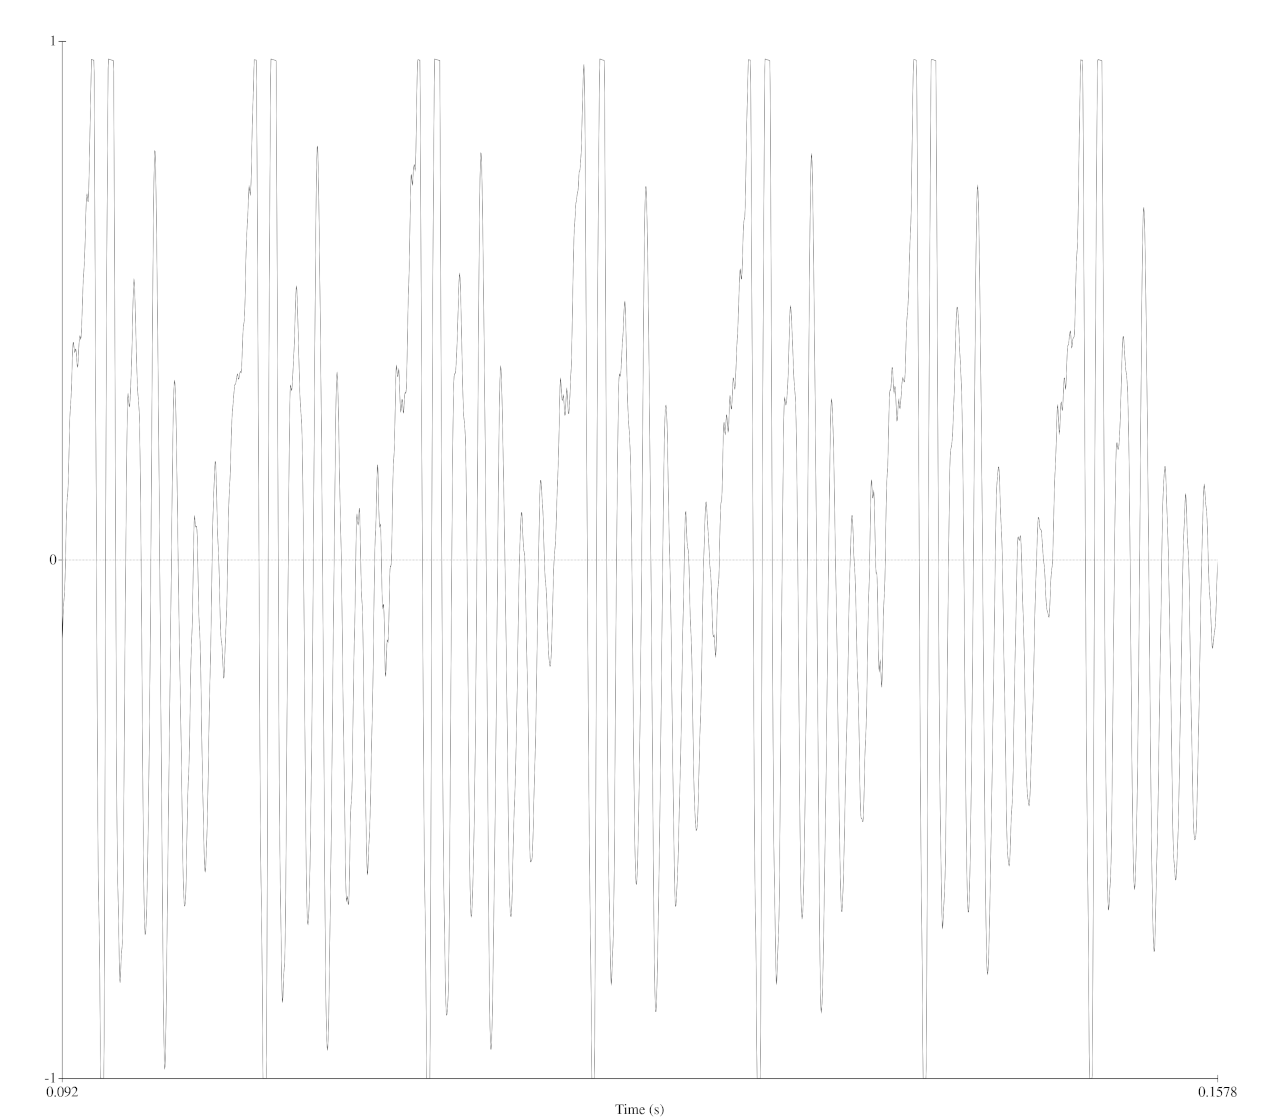
\includegraphics[width=0.75\textwidth]{images/ondaa}
	\caption{Onda de [aː].}
	\label{fig:ondaa}
\end{figure}

Con esto, emprendemos la tarea pertrechados de los medios técnicos apropiados \parencite{boersma2022}: analizar un \textit{sonograma}\index{sonograma} (\Cref{fig:sonogramas}), que es el gráfico que representa las variaciones de la frecuencia en el eje de ordenadas a lo largo del tiempo en el de abscisas. El sonograma se filtra según un determinado rango de frecuencias para examinar diferentes aspectos del sonido. Así, un sonograma \textit{de banda estrecha}\index{sonograma!de banda estrecha} como el de \Cref{fig:anarrow} es más adecuados para observar los armónicos de la onda, más difíciles de discernir en uno \textit{de banda ancha}\index{sonograma!de banda ancha} como el de \Cref{fig:awide}, que, por el contrario, ofrece una perspectiva más amplia del sonido \parencite[95-96]{clegg2018}. Las franjas más oscuras corresponden a los formantes\index{formante} en el sonograma de banda estrecha o a sus agrupaciones en el de banda ancha. En el ejemplo, que representa el sonido \ipa{/a/}, la frecuencia fundamental se encuentra alrededor de los 108,65 Hz, el primer formante $F_1$ tiene una frecuencia ocho veces mayor, el segundo $F_2$ diez veces mayor, el tercero $F_3$ veinticuatro veces mayor y el cuarto $F_4$  veinticinco veces más.

\begin{figure}[!ht]
	\centering
	\begin{subfigure}{0.49\textwidth}
		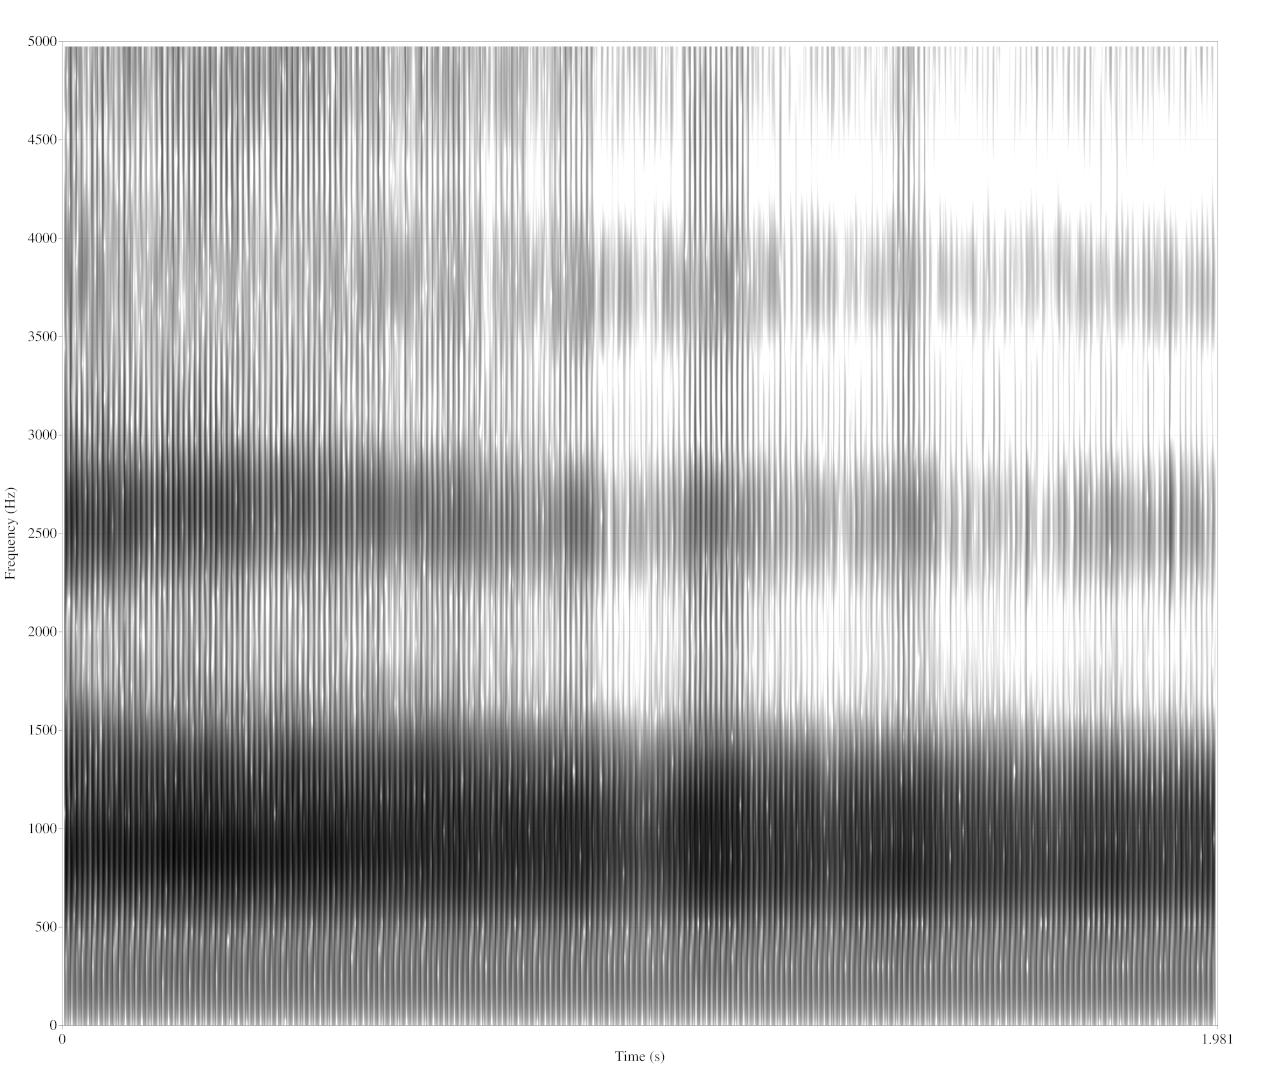
\includegraphics[width=\textwidth]{images/awidex}
		\subcaption{Banda ancha.}
		\label{fig:awide}
	\end{subfigure}
	\begin{subfigure}{0.49\textwidth}
		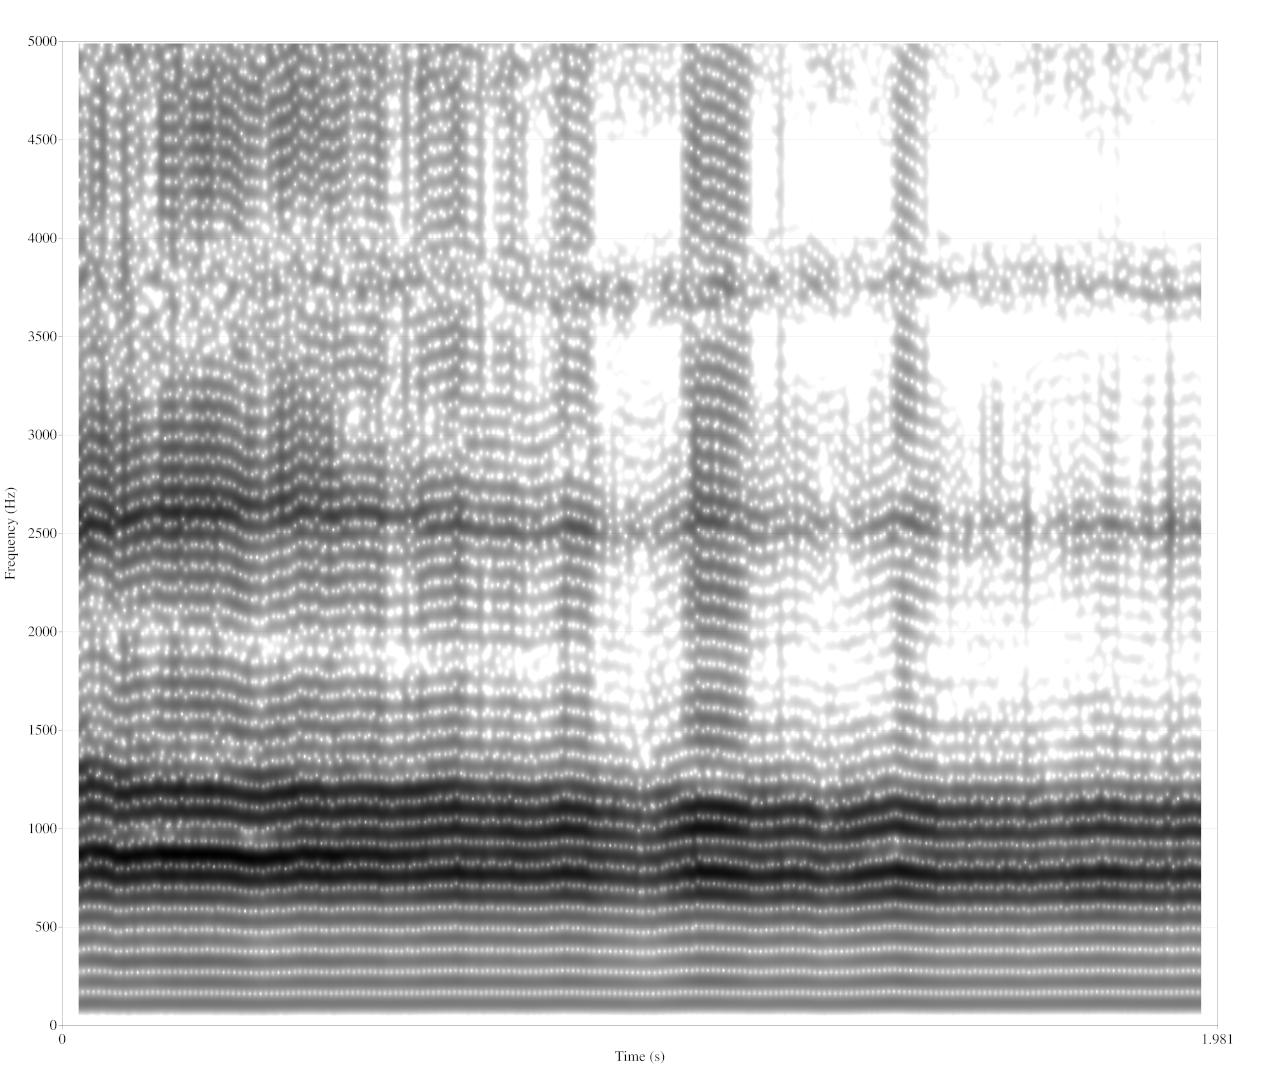
\includegraphics[width=\textwidth]{images/anarrowx}
		\subcaption{Banda estrecha.}
		\label{fig:anarrow}
	\end{subfigure}
	\caption{Espectrogramas de [aː].}
	\label{fig:sonogramas}
\end{figure}


Estos formantes\index{formante}, de forma especial el primero y el segundo, facilitan la distinción entre las vocales. El primer formante $F_1$ viene definido por la manera de articulación, ya que la frecuencia de este tiene una relación proporcional con la apertura bucal y, por el contrario,  cuanto más cerrada se encuentre la boca, tanto más bajo será el formante. El segundo formante lo determina el lugar de articulación, de manera que cuanto más anterior sea la articulación, más alta será la frecuencia y viceversa, cuanto más posterior sea el sonido, más baja la frecuencia de $F_2$. De esta manera, los valores de $F_1$ de las vocales españolas serían aproximadamente los representados en la Tabla \ref{tab:formantvocales} \parencite[101]{clegg2018}.

\begin{table}[!ht]
	\centering\small
	\begin{tikzpicture}[font=\footnotesize, domain=0:] %, every node/.style={fill, circle, inner sep = 1pt}]
    \begin{axis}[
    	 /pgf/number format/.cd,
    	use comma,
    	1000 sep={},
      width = 0.8\textwidth,
      axis lines = middle,
      xmin=700,
      xmax=2300,
      ymin=200,
      ymax=900,
      ylabel style={at=(current axis.below origin), anchor=south, , yshift=-0.5cm},
      x dir=reverse,
      y dir=reverse,  
      %label style={at=(current axis.below origin), anchor=south},
      xlabel style={at=(current axis.left of origin), anchor=west, xshift=-0.5cm},
      %xticklabel pos=right,
      %ylabel near ticks,
      % yticklabel pos=right,
      enlargelimits = true,
      xlabel={$F_2$},
      ylabel={$F_1$}],
    ]    
    \node (i) at (2174,315) {\large$i$};
    \node (e) at (1895,501) {\large$e$};
     \node (a) at (1300,762) {\large$a$};
    \node (o) at (966,501) {\large$o$};
     \node (u) at (836,315) {\large$u$};
    \end{axis}


  \end{tikzpicture}

	\caption{Formantes $F_1$ y $F_2$ de las vocales (Hz).}
	\label{tab:formantvocales}
\end{table}

La relación con el trapecio articulatorio se hace más evidente si disponemos estos valores en un gráfico. Como muestra \Cref{fig:formantvocales}, la posición de los sonidos según las frecuencias de sus dos primeros formantes\index{formante} está relacionada con el trapecio articulatorio.

Para interpretar sonidos consonánticos no basta con identificar el modo y lugar de articulación, sino que una descripción precisa requiere conocer el estado de las cuerdas vocales; esto es, hallar el grado de intervención de este órgano porque su vibración determina si la consonante es \textit{sonora}\index{consonante!sonora} o \textit{muda}\index{consonante!muda}.

Las oclusivas\index{consonante!oclusiva} se identifican por presentar un periodo de ausencia de energía durante la fase productiva, en el que no hay expulsión de aire. En las fricativas\index{consonante!fricativa}, la energía se extiende por el gráfico a lo largo del tiempo de producción. Las africadas\index{consonante!africada} están caracterizadas por la producción en dos fases, una primera oclusiva seguida de otra de liberación africada. Las consonantes nasales\index{consonante!nasal} y laterales\index{consonante!lateral}, conocidas también como \textit{sonorantes}\index{consonante!sonorante}, presentan formantes\index{formante} al modo de los sonidos vocálicos, aunque estos no son tan intensos. Las vibrantes\index{consonante!vibrante} se distinguen por las interrupciones de la onda sonora, poseyendo varias las múltiples\index{consonante!vibrante!múltiple} y una las simples \index{consonante!vibrante!simplel} \parencite[101-102]{clegg2018}.

\begin{figure}[!ht]
	\centering\small
	\begin{tikzpicture}[font=\footnotesize, domain=0:] %, every node/.style={fill, circle, inner sep = 1pt}]
    \begin{axis}[
    	 /pgf/number format/.cd,
    	use comma,
    	1000 sep={},
      width = 0.8\textwidth,
      axis lines = middle,
      xmin=700,
      xmax=2300,
      ymin=200,
      ymax=900,
      ylabel style={at=(current axis.below origin), anchor=south, , yshift=-0.5cm},
      x dir=reverse,
      y dir=reverse,  
      %label style={at=(current axis.below origin), anchor=south},
      xlabel style={at=(current axis.left of origin), anchor=west, xshift=-0.5cm},
      %xticklabel pos=right,
      %ylabel near ticks,
      % yticklabel pos=right,
      enlargelimits = true,
      xlabel={$F_2$},
      ylabel={$F_1$}],
    ]    
    \node (i) at (2174,315) {\large$i$};
    \node (e) at (1895,501) {\large$e$};
     \node (a) at (1300,762) {\large$a$};
    \node (o) at (966,501) {\large$o$};
     \node (u) at (836,315) {\large$u$};
    \end{axis}


  \end{tikzpicture}

	\caption{Formantes $F_1$ y $F_2$ de las vocales (Hz).}
	\label{fig:formantvocales}
\end{figure}	

La posición de la articulación varía con el  modo en que esta se produce\index{articulación!modo}. Para las oclusivas, hay que observar las transiciones entre formantes\index{formante} de las vocales en contacto con la consonante, ya que estas tienen formas propias para cada sonido. En el caso de las fricativas, hay que tener en cuenta además la energía acústica empleada en su producción \parencite[102]{clegg2018}. Determinar la sonoridad de la consonante presenta menos dificultades. La vibración de las cuerdas vocales se aprecia en el sonograma de banda ancha, que muestra estrías verticales en las sonoras\index{consonante!sonora}, de las que carecen las sordas\index{consonante!sorda} \parencite[102]{clegg2018}. 



%\begin{table}[!ht]
	%\centering\small
	%\input{tables/formantnasales}
	%\caption{Formantes de las consonantes nasales y laterales  (Hz).}
	%\label{tab:formantnasales}
%\end{table}



\section{El sistema fonológico}
La unidad fonológica mínima es el \textit{fonema}\index{fonema}, que Jakobson \parencite*[231]{jakobson1962a} define como «un conjunto de propiedades sonoras concurrentes usadas en una lengua dada para distinguir palabras de significado distinto». Esto es, los fonemas deben servir al hablante para discriminar entre una palabra y otra según el principio\index{principio de pertinencia} de pertinencia\index{pertinencia|see{principio de pertinencia}}; esto es, lo que distingue entre las propiedades esenciales y las contingentes en la diferenciación de significados. En palabras de Martinet \parencite*[45]{martinet1970}, \blockquote{le principe de pertinence nous permet de distinguer ce	qui, dans chaque langue ou chaque usage, est essentiel parce que distinctif, et ce qui est contingent, c'est-à-dire déterminé par le contexte ou diverses circonstances}.

Un fonema, sin embargo, no corresponde a un sonido único, ya que admite varias realizaciones fonéticas con diferentes sonidos. Estas dependen del estilo de habla o del contexto fonético concreto en el que aparecen. La diferencia entre sonidos responde a factores externos y no influye en la distinción de significados, por lo que esos sonidos no son sino variantes de un fonema dado \parencite[231]{jakobson1962a} o \textit{alófonos}\index{alófono}.  Así, los sonidos \ipa{[β]} y \ipa{[b]} son realizaciones diferentes del mismo fonema \ipa{/b/}, y se selecciona una u otra dependiendo del contexto fonético donde se produzca el fonema. Por lo tanto, aunque \textit{abocar} se pronuncie \ipa{[aβoˈkaɾ]} y \textit{embozar} \textipa{[emboˈθaɾ]}, la diferencia no se percibe como un sonido diferente, por lo que hablamos de un único fonema \ipa{/b/}.

Esto obliga a establecer criterios para distinguir entre un fonema y una realización alternativa de este. Trubetzkoy \parencite*[42-46]{trubetzkoy1939} propone para ello las siguientes cuatro reglas:
\begin{enumerate}[label=\Roman*]
	\item «Cuando dos sonidos de la misma lengua se dan exactamente en el mismo contexto fónico y pueden intercambiarse sin provocar una diferencia en el significado intelectual de la palabra, esos dos sonidos son solo dos variantes facultativas de un único fonema» \parencite[p. 42; traducción propia]{trubetzkoy1939}. 
	\item «Cuando dos sonidos se dan exactamente en la misma posición fónica y no pueden ser intercambiados sin alterar el significado de la palabra o hacerla irreconocible, estos dos sonidos son realizaciones de dos fonemas distintos» (p. 44; traducción propia).
	\item  «Cuando dos sonidos acústica o articulatoriamente emparentados de una lengua no se dan nunca en el mismo contexto fónico, se consideran como variantes combinatorias del mismo fonema» (pp. 44-45; traducción propia).
	\item «Dos sonidos, aunque cumplan las condiciones de la regla III, no deben ser considerados variantes del mismo fonema en la lengua en cuestión si estos pueden darse en posiciones adyacentes, esto es, como grupo fónico de una secuencia de sonidos en aquellas posiciones en las que, también, uno de los sonidos también puede aparecer aislado» (p. 46; traducción propia).
\end{enumerate}
Estas reglas se ven mejor mediante casos prácticos. Verbigracia, la regla I se aplica a los sonidos \ipa{[h]} y \ipa{[s]} del español meridional como alófonos de /s/. Vemos que \ipa{[ˈkasah]} y \ipa{[ˈkasas]} son formas intercambiables de realizar \textit{casas}. El ejemplo que dimos arriba de \ipa{/ˈgata/} y \ipa{/ˈkata/} es representativo de la regla II. La regla III alude a casos como el de los alófonos \ipa{[d]} y \ipa{[ð]} del fonema \ipa{/d/}, pues el primer sonido únicamente aparece detrás de pausa, consonante nasal o lateral, mientras que el segundo lo hace en el resto de casos, no haciéndolo en los que afectan al primero. Así, tenemos \ipa{[esˈpalda]} y \ipa{[esˈpaða]}. La regla IV es relevante en ejemplos como el de la  semiconsonante\index{vocoide} \ipa{[w]} y la semivocal \ipa{[u̯]} como variantes combinatorias de \ipa{/u/}, ya que, además de cumplir la regla III, no aparecen en posición contigua a \ipa{[u]}.
 
Los sonidos lingüísticos, empero, en muy contadas ocasiones aparecen aislados. Por el contrario, suelen ser el resultado de la combinación articulada de una secuencia. Esto no es impedimento para que se dé el caso opuesto. Lo que en apariencia son dos fonemas individuales contiguos pueden no serlo, sino constituir solamente uno. Por ello, se hace necesario distinguir entre fonemas simples adyacentes y fonemas complejos constituidos de una serie de sonidos. Trubetzkoy propone las siguientes seis reglas para hacerlo:
\begin{enumerate}[label=\Roman*]
	\item «Solo puede ser considerado como realización de un fonema individual la unión de sonidos cuyos componentes no se reparten entre dos sílabas en la lengua en cuestión» \parencite[p. 50; traducción propia]{trubetzkoy1939}.
	\item «Solo puede ser considerado como realización de un fonema individual una unión de sonidos producida por un movimiento articulatorio homogéneo o a través de la disolución progresiva de un complejo articulatorio»  (p. 51; traducción propia).
	\item «Solo puede ser considerado como realización de un fonema individual una unión de sonidos cuya duración no sobrepase la duración de la realización de otros fonemas de la lengua en cuestión» (p. 53; traducción propia).
	\item «Una unión de sonidos potencialmente monofonemática —esto es, que cumple las reglas I, II y III— debe ser considerada realización de un único fonema si se trata como un fonema individual\footnote{La tautología es del original: «\begin{textgerman}Eine potentiell monophonematische Lautverbindung (d.i. den Forderungen der Regel I—III entsprechende) Lautverbindung muß als Realisation eines einzigen Phonems gewertet werden, wenn sie als Einzelphonem behandelt wird [...]\end{textgerman}».}, esto es, si se da en aquellas posiciones en las que grupos fonemáticos no pueden ocurrir en la lengua en cuestión» (p. 53; traducción propia).
		\item «Una combinación de sonidos que cumpla las reglas de I a III debe ser considerada la realización de un fonema si esto produce simetría en el sistema fonológico»\footnote{He recurrido a otra edición \parencite{trubetzkoy1969} porque la regla V no aparece en el texto original \parencite{trubetzkoy1939}, pasando de la IV a la elaboración de la V, pero sin llegar a enunciarla.} \parencite[p. 59; traducción propia]{trubetzkoy1969}.
	\item «Si un componente de una unión fonemática potencial no pude ser evaluada como variante combinatoria de algún otro fonema de la lengua en cuestión, la unión de sonidos debe ser interpretada como un fonema individual» \parencite[p. 56; traducción propia]{trubetzkoy1939}. 
\end{enumerate}

Podemos aclarar estos puntos con algunos casos ilustrativos. Vemos que en el fonema \ipa{/ʧ/} del español hay una obstrucción que se libera para deshacerse luego en la fricativa. Sin embargo, sus componentes \ipa{[t]} y \ipa{[ʃ]} no se dividen entre dos sílabas como sí ocurre en otros idiomas como el alemán. Compárense las palabras de sendas lenguas \textit{hucha} y \textit{Lautschrift}, pronunciadas respectivamente como \ipa{/ˈu.ʧa/} y \textipa{/ˈlaʊt.ʃrIft/}. De esta manera, atendiendo a las reglas I y II, \ipa{[tʃ]} constituirían un único fonema complejo /\texttoptiebar{tʃ}/ en español pero dos fonemas simples \ipa{/t/} y \ipa{/ʃ/} en alemán. El equivalente a estos fonemas germanos lo tenemos en castellano con  \ipa{/ks/}, la pronunciación de \textit{x}. En \textit{facsímil}, por ejemplo, se distribuye en dos sílabas como \ipa{/fak.ˈsi.mil/}. Con respecto a la regla III, se ve en \textit{preeminente} que no se interpreta como \textipa{/pre:mi.ˈnen.te/}, pues contravendría la homogeneidad silábica del español —sin olvidar que la cantidad no es contrastiva en esta lengua—. Sobre la regla IV, Trubetzkoy propone el ejemplo de palabras alemanas como \textit{Zwei} o \textit{Pflanze}, que parecen contravenir la regla de que el alemán solo permite en ataque los segmentos de tres consonantes \ipa{[ʃtr]}, \ipa{[ʃpl]} y \ipa{[ʃpr]}; de esta manera, parece obligado evaluar los grupos \ipa{[ts]} y \ipa{[pf]} en ataque como fonémicos.

Partiendo de lo expuesto, recabamos el inventario de fonemas de una lengua dada. Para ello necesitamos, además, determinar el \textit{contenido fónico}\index{fonema!contenido fónico} de cada uno de ellos, esto es, sus propiedades distintivas. Dicho de otra manera, se requiere encontrar aquellas características comunes a todas las variantes de un mismo fonema \parencite[59]{trubetzkoy1939}. Por ejemplo, si describimos el fonema \ipa{/d/} como plosivo\index{consonante!plosiva}, sería adecuado para su realización \ipa{[d]}, pero excluiría otras realizaciones tan válidas como el aproximante\index{consonante!aproximante} \ipa{[ð]}. Por el contrario, resultaría inadecuado describirla solo como dental porque, aunque ambos alófonos lo cumplen, también lo hacen realizaciones de otros fonemas, como  \ipa{[t]} y \ipa{[θ]}. Es necesario, por lo tanto, indicar los rasgos relevantes: en el caso de \ipa{/d/}, dental sonoro.

El nivel fonológico constituye el material principal que conforma  los cimientos sobre los que se asienta la métrica. Sin embargo, no hay que dejar de lado del todo algunos aspectos de la lengua que hunden sus raíces en la fonética, de forma muy especial en el territorio de las vocales, donde la propiedad silábica del fonema representa un papel protagonista en la medida del verso. Debemos, pues, dilucidar el modo en el que el contexto fónico afecta a los fonemas individuales si esto altera la sustancia métrica del verso. Debemos hacer notar que esta disolución de las lindes entre los niveles fonético y fonológico no es extraña a la disciplina. Tanto Quilis \parencite*{quilis2019} como Alarcos Llorach, por ejemplo, clasifican hasta cierto punto los fonemas según criterios fonéticos.  Este último lo justifica arguyendo que \blockquote[{\cite[54]{alarcos1964}}]{hay que tener presente la diferencia entre fonología y fonética, a pesar de que en la práctica fonológica se utiliza la nomenclatura fonética por simplicidad. Esta está basada en las características articulatorias de los sonidos, aunque haya entre sus términos algunos puramente impresionísticos; por ser bien conocida, ofrece ventajas para la comprensión el aprovecharla en fonología.}

Una vez establecido el marco en el que definiremos el sistema fonológico y hechas las debidas prevenciones, queda por definir una serie mínima de rasgos identificativos\index{rasgo distintivo} u oposiciones\index{oposición}. Estos rasgos no solo deben distinguir a los términos de la oposición, sino que tienen que representar una cualidad común a ambos \parencite[68-87]{trubetzkoy1969}. Esto servirá para organizar el repertorio de todos los fonemas disponibles en una lengua en un sistema fonológico.

Atendiendo a la relación con el sistema fonológico, se distingue entre \textit{oposiciones bilaterales}\index{oposición!bilateral} y \textit{multilaterales}\index{oposición!multilateral}\footnote{También se conocen como \textit{unidimensionales} y \textit{pluridimensionales}, respectivamente.}, y \textit{oposiciones proporcionales}\index{oposición!proporcional} y \textit{aisladas}\index{oposición!aislada}. Llamamos \textit{oposiciones bilaterales} a aquellas en las que el \textit{tertium comparationis} es particular de los dos términos y no se da en otro término del mismo sistema fonológico. Las \textit{oposiciones multilaterales}, por su parte, son aquellas en las que la base de la comparación se da en otros términos. Quilis \parencite*[36]{quilis2019} ejemplifica la relación bilateral con los fonemas \ipa{/k/}-\ipa{/x/} del español, cuyas propiedades compartidas (orales, velares, sordas) no aparecen juntas en ningún otro fonema, de la misma manera que \ipa{/e/}-\ipa{/i/} (vocales, sonoras, anteriores). Como ejemplo de multilateralidad, Quilis cita /b/-/d/, ya que sus rasgos comunes\index{rasgo distintivo} (consonantes, oclusivas, orales, sonoras) se dan también en /b/-/g/ o /d/-/g/.

En las \textit{oposiciones proporcionales}\index{oposición!proporcional}, la relación que se da entre sus términos se encuentra en los de otra oposición, mientras que los términos de las \textit{oposiciones aisladas} tienen una relación única en el sistema fonológico. De esta manera, /p/-/b/ es proporcional porque la misma relación se da en /t/-/d/ y /k/-/g/, mientras que la oposición /r/-/l/ es aislada, ya que la relación no aparece en ningún otro par del sistema. 

Según las relaciones entre los términos, las oposiciones son \textit{privativas}, \textit{graduales} o \textit{equipolentes}. Las \textit{oposiciones privativas}\index{oposición!privativa} son de naturaleza binaria y se caracterizan por la presencia o ausencia de una marca. El término que presenta la marca se denomina \textit{término marcado}\index{término!marcado} y, de forma análoga, el que no la presenta se llama \textit{no marcado}\index{término!no marcado}. Por ejemplo, si consideramos el rasgo sonoridad\index{rasgo distintivo}, en la oposición /p/-/b/, /b/ será el término marcado (sonoridad: +) y /p/ el no marcado (sonoridad: $-$). Por el contrario, las \textit{oposiciones graduales}\index{oposición!gradual} presentan la distinción como un grado no binario. La apertura de las vocales es un ejemplo de este tipo de oposiciones. Así, /i/ es más cerrada que /e/, que a su vez es más cerrada que /a/. Las \textit{oposiciones equipolentes}\index{oposición!equipolente} son aquellas cuyos miembros son equivalentes. Esto es, no han de ser consideradas ni privativas ni graduales, por ejemplo /p/-/k/ o /i/-u/.

Las oposiciones fonológicas también se caracterizan mediante su poder distintivo en \textit{constantes}\index{oposición!constante} o \textit{neutralizables}\index{oposición!neutralizable}. Las primeras se realizan siempre sin que tenga relevancia la posición que ocupen, mientras que las segundas no se dan en ciertas posiciones. En este último caso, la posición donde se mantiene la distinción se denomina \textit{de pertinencia}\index{posición!de pertinencia}, mientras que aquella en la que se neutraliza se llama \textit{de neutralización}\index{posición!de neutralización}. Por ejemplo, /s/-/θ/ serían constantes en \textit{español de Castilla}\footnote{Por comodidad, me referiré al español de Castilla para denotar las variedades peninsulares septentrionales que se acercan a lo que, con todas las precauciones, podríamos llamar \textit{español estándar}.} porque no pierden capacidad distintiva según su posición, como se ve en \textit{casa} /ˈka.sa/ y \textit{caza} /ˈka.θa/ o \textit{hez} /eθ/ y \textit{es} /es/. Por el contrario, /r/-/ɾ/ solo funcionan en posición prenuclear, de forma que mientras que \textit{perro} /ˈpe.ro/ y \textit{pero} /ˈpe.ɾo/ son distintas fonológicamente,  /baɾ/ y /bar/ son dos formas de pronunciar la misma palabra \textit{bar}.

Los rasgos distintivos\index{rasgo distintivo} varían según desde qué perspectiva fonética se aborde la fonología. Quilis \parencite*[44]{quilis2019} menciona la \textit{fonética sincrónica}\index{fonética!sincrónica}, \textit{diacrónica}\index{fonética!diacrónica}, \textit{articulatoria}\index{fonética!articulatoria}, \textit{acústica}\index{fonética!acústica}, \textit{auditiva}\index{fonética!auditiva} y \textit{psicológica}\index{fonética!psicológica}. Este estudio se vale ante todo de la fonética articulatoria\index{fonética!articulatoria} como marco descriptivo del sistema fonológico. Sin embargo, dadas las dificultades que presentaría examinar físicamente a los hablantes para controlar la producción del sonido, nos apoyaremos en la fonética acústica\index{fonética!acústica} para contrastar muestras de sonidos mediante la observación de sus espectrogramas. Esto permite, por un lado, obtener de manera sencilla las muestras como archivos de audio y, por otra parte, examinarlos a fondo con el \textit{software} adecuado\footnote{En nuestro caso, Praat \parencite{boersma2022}.}. Así pues, habremos de establecer estos marcos fonéticos descriptivos. 

Los rasgos distintivos\index{rasgo distintivo} en se dividen en \textit{prosódicos}\index{rasgo distintivo!prosódico} e \textit{intrínsecos}\index{rasgo distintivo!intrínseco} o \textit{inherentes}\index{rasgo distintivo!inherente|see {intrínseco}}. Todos los fonemas poseen estos últimos, pero los primeros son exclusivos de los fonemas constituyentes de núcleo silábico \parencite[111]{quilis2019}.

Desde un punto de vista acústico, se distinguen diferentes rasgos\index{rasgo distintivo}. Alarcos~Lorach~\parencite*[85]{alarcos1964} propone \textit{vocálico}/\textit{no vocálico} y \textit{consonántico}/\textit{no consonántico}, que se basan en el formante\index{formante} generador de la onda sonora y la presencia o ausencia de obstáculo en el canal bucal. Permiten discriminar entre fonemas vocales, consonantes, líquidos y glotales;  \textit{denso}/\textit{difuso}, basándose en la proporción de las cavidades bucofaríngeas; \textit{grave}/\textit{agudo}, junto a los rasgos precedentes\index{rasgo distintivo},  revela la ubicación de los fonemas, \textit{bemolizado}/\textit{normal} y  \textit{sostenido}/\textit{normal}, que dependen del timbre del resonador bucal y distinguen series paralelas de sonidos con timbre modificado; \textit{nasal}/\textit{oral}, según se emplee la nariz o la boca como cavidad resonadora; \textit{tenso}/\textit{flojo}, en función de la tensión de los órganos fonadores, que indica propiedades prosódicas de las vocales y distingue entre consonantes fuertes y débiles;  \textit{sonoro}/\textit{sordo}, que viene determinado por la vibración de la glotis y actúa en combinación con el rasgo precedente\index{rasgo distintivo}; \textit{continuo}/\textit{interrupto} y  \textit{estridente}/\textit{mate}, que dependen de si el ataque es abrupto o hay una interrupción en el flujo del aire, así como de la aproximación de los órganos fonadores y \textit{recursivo}/\textit{infraglotal}, determinado por la existencia de cierre glotal al final del sonido y diferencia el modo en que la glotis interviene en la expulsión del aire. 

Quilis \parencite*[165-167]{quilis2019}, por su parte, distingue para los sonidos vocálicos entre \textit{compactos} y \textit{no compactos}, siendo \textit{difuso} y \textit{no difuso} propiedades de los últimos. Asimismo, desdobla grave/agudo en \textit{grave} y \textit{no grave}, pudiendo aquellos que se hallan en el segundo caso subdividirse en \textit{agudo} y \textit{no agudo}. Además, hace distinciones más finas, añadiendo \textit{denso}/\textit{no denso}, \textit{difuso}/\textit{no difuso}, \textit{grave/no grave} y \textit{agudo/no agudo}.

\section{Neutralización}
El fenómeno de la neutralización\index{neutralización} consiste en la desaparición del contraste fonémico en ciertos entornos fonológicos, bien por la pérdida de una característica propia del fonema o por la adquisición de otra ajena a este. 

\citeauthor{alarcos1964}~\parencite*[97-99]{alarcos1964} describe dos tipos de neutralización, una \textit{condicionada por el contexto}\index{neutralización!condicionada} y otra \textit{exigida por la estructura}, que es \textit{interna}\index{neutralización!interna} del sistema. Mientras que la primera ocurre como respuesta a fonemas cercanos, como en el caso de una consonante nasal ante otra consonante, la segunda la determina la posición, como en las vibrantes a final de sílaba. La neutralización condicionada es \textit{disimilativa}\index{neutralización!disimilativa} si el fonema pierde su carácter distintivo por la influencia de otro con un rasgo distintivo semejante o \textit{asimilativa}\index{neutralización!asimilativa} si lo pierde por contacto con otros fonemas carentes de este. La neutralización interna, por su parte, se divide entre la \textit{centrífuga}\index{neutralización!centrífuga} y la \textit{reductiva}\index{neutralización!reductiva}. La neutralización centrífuga es aquella que ocurre en los límites de palabra o sílaba, mientras que la reductiva es la que se da en todas las sílabas menos en la culminante o acentuada.

Este suele darse con mayor frecuencia en la distensión silábica de final de sílaba \parencite[180]{alarcos1964}, lo que, a efectos prácticos, reduce su alcance a las consonantes que suelen darse en tal posición. En español, la neutralización es especialmente notable en coda. En lo que a nuestro estudio respecta, la asimilación en coda en la rima podría determinar la diferencia entre consonancia y asonancia. Esto, sin embargo, solo sucedería en casos tan excepcionales que podemos pasarlo por alto. No obstante, hemos de mencionarlo como una posibilidad teórica.

\section{Fonemas del español}
\subsection{Sonidos vocálicos}
Desde las gramáticas más primitivas de Grecia y la India, los estudiosos del lenguaje han divido los sonidos entre consonantes y vocales. Esta clasificación no es arbitraria, ya que se ha comprobado que hay diferencias articulatorias que, a su vez, tienen consecuencias en el plano acústico. Las vocales se producen por una acción articulatoria fuerte, en la que se alcanza una máxima apertura, mientras que una acción articulatoria débil produce el efecto contrario \parencite[141-143]{quilis2019}. En lo que concierne a este trabajo, los sonidos vocálicos son fundamentales, ya que con ellos se contarán las sílabas. Por esta razón debemos identificarlos y caracterizarlos. Sin embargo, aunque todos los núcleos silábicos son vocálicos, no todas las vocales  son necesariamente silábicas, por lo que será preciso, en ese caso, no solo caracterizarlas, sino identificar sus propiedades físicas para contar con criterios para resolver casos dudosos.

Podemos caracterizar los sonidos vocálicos, al igual que los consonánticos, por el modo\index{articulación!modo} y por el punto de articulación\index{articulación!punto}. El modo de articulación se refiere a la apertura que deja la lengua en la cavidad bucal, mientras que el punto de articulación, al contrario que las consonantes, no es respecto a cierres o puntos de contacto, sino a la región palatal a la que se aproxima el dorso lingual. Por el modo de articulación, distinguimos entre vocales altas, medias y bajas.

La lengua castellana se caracteriza por la homogeneidad del repertorio vocálico en todas sus variedades dialectales. Así se ha descrito tradicionalmente y la fonética moderna tampoco ha encontrado más vocales a nivel fonológico, por lo que limita a describir las diferentes realizaciones fonéticas de los fonemas. En la conciencia lingüística del hablante existen tan solo cinco vocales: \textit{a}, \textit{e}, \textit{i}, \textit{o} y \textit{u}. En este caso, sí existen alófonos que dependen sobre todo del contexto fónico del segmento dado \parencite[32]{navarrotomas1946}. Las realizaciones de \textipa{/a/}, \textipa{/e/} y \textipa{/o/} son siempre vocálicas puras y son capaces de formar núcleo vocálico, mientras que, como detallamos abajo, \textipa{/i/} y \textipa{/u/} se realizan como vocales puras cuando son tónicas o cuando son átonas, pero no están en contacto con otra vocal \parencite[152-153]{alarcos1964}.

Si nos situamos en el trapecio bucal, el fonema /i/ es articulatoriamente \textit{alto} y el más \textit{anterior} del repertorio español. Es acústicamente \textit{vocálico}, \textit{no consonántico}, \textit{no compacto}, \textit{difuso}, \textit{no grave} y \textit{agudo}. Presenta dos realizaciones en distribución complementaria. La primera es la oral regular [i] (\textlangle{}piso\textrangle{} [ˈpiso]). La segunda es la nasalizada [ĩ], cuando /i/ se encuentra entre pausa y consonante nasal (\textlangle{}instante\textrangle{} [ĩnsˈtan̪te]) o entre dos consonantes nasales (\textlangle{}mimo\textrangle{} [ˈmĩmo]) \parencite[168-169]{quilis2019}.

También localizada articulatoriamente en una posición anterior, aunque a una altura \textit{media}, se encuentra el fonema /e/. Acústicamente, se describe como vocálico, no consonántico, no compacto, \textit{no difuso}, no grave y agudo. Tiene también dos realizaciones, una oral regular \ipa{[e]} (\textlangle{}peso\textrangle{} \ipa{[ˈpeso]}), y otra  nasal \ipa{[ẽ]} cuando /e/ se encuentra entre pausa y consonante nasal (\textlangle{}encono\textrangle{} \ipa{[ẽŋˈkono]}) o entre dos consonantes nasales (\textlangle{}memo\textrangle{} \ipa{[ˈmẽmo]}) \parencite[169]{quilis2019}.

El fonema vocálico más \textit{central} y \textit{bajo} es \ipa{/a/}. Acústicamente, es vocálico, no consonántico, \textit{compacto}, \textit{denso}, no grave y \textit{no agudo}. También \ipa{/a/} presenta dos alófonos en distribuciones complementarias, uno nasal [ã] cuando se halla entre una pausa y una consonante nasal (\textlangle{}antena\textrangle{} \ipa{[ãn̪ˈtena]}) y otra regular \ipa{[a]} (\textlangle{}casa\textrangle{} \ipa{[ˈkasa]}) en el resto  \parencite[169]{quilis2019}.

El fonema /o/ es medio y \textit{posterior}. Conforme a sus propiedades acústicas, es vocálico, no consonántico, no compacto, no difuso, \textit{grave}. De la misma manera, \ipa{/o/} tiene dos realizaciones, una oral regular \ipa{[o]} (\textlangle{}vaso\textrangle{} \ipa{[ˈBaso]}) y otra  nasal \ipa{[õ]}, cuando /o/ se encuentra entre pausa y consonante nasal (\textlangle{}oncología\textrangle{}  \ipa{[õŋkoloˈxia]}) o entre dos consonantes nasales (\textlangle{}nona\textrangle{} \ipa{['nõna]}) \parencite[169]{quilis2019}.

Por último, el fonema \ipa{/u/} es articulatoriamente alto y posterior. Se caracteriza acústicamente por ser vocálico, no consonántico, no compacto, difuso, grave. Al igual que el resto de vocales, \ipa{/u/} también tiene dos realizaciones en distribución complementaria, una oral regular \ipa{[u]} (\textlangle{}huso\textrangle{} \ipa{['uso]}) y otra  nasal \ipa{[ũ]}, cuando \ipa{/u/} se encuentra entre pausa y consonante nasal (\textlangle{}ungüento\textrangle{} \ipa{[ũŋˈgwen̪to]}) o entre dos consonantes nasales (\textlangle{}mundo\textrangle{} \ipa{[ˈmũn̪do]}) \parencite[170]{quilis2019}.

Esto se resume en  que, considerando la apertura\index{articulación!modo}, el español tiene dos vocales \textit{altas}\index{vocal!alta} o \textit{cerradas}\index{vocal!cerrada}, aquellas en que la lengua se aproxima al paladar duro o al paladar blando. Estos son los fonemas \ipa{/i/} y \ipa{/u/}. También cuenta con dos vocales \textit{medias}\index{vocal!media}, en las que la lengua se separa de la bóveda del paladar para posicionarse en medio de la cavidad bucal. Estas son \ipa{/e/} y \ipa{/o/}. El español solo posee una vocal \textit{baja}\index{vocal!baja} o \textit{abierta}\index{vocal!abierta}, esto es, cuando se produce una apertura máxima al alejarse la lengua del paladar en el mayor grado colocándose en la parte inferior de la cavidad bucal. Esta es /a/ \parencite[146-147]{quilis2019}.

Según el punto  de articulación\index{articulación!punto}, el español dispone de vocales anteriores, centrales y posteriores. Las vocales anteriores\index{vocal!anterior}, aquellas que se producen cuando la lengua se halla en la parte frontal de la cavidad bucal, son /i/ y /e/. En español solo aparece \textipa{/a/} como vocal media, en la que el dorso de la lengua se halla en la región del paladar medio\index{vocal!central}. Las vocales posteriores del español, en las que el posdorso de la lengua se acerca a la región posterior de la cavidad bucal, son /u/ y /o/ \parencite[147-148]{quilis2019}. En lo relativo a sus cualidades acústicas, todas las vocales del repertorio fonológico del español son \textit{vocálicas} y \textit{no consonánticas}.

\begin{table}[h!]
	\centering\small
	\begin{tabular}{lccc}
		\toprule	
		& \textbf{Anterior} & \textbf{Central} & \textbf{Posterior}  \\
		\midrule
		\textbf{Cerrada}          &  i  &   & u    \\
		\textbf{Media}       & e̞  &   &o̞   \\
		\textbf{Abierta}       &     & ä  &   \\
		\bottomrule
	\end{tabular}
	\caption{Fonemas vocálicos del español.}
	\label{tab:vocales}
\end{table}


Así pues, la lengua española cuenta con cinco vocales\index{vocal} que se distinguen entre sí por oposición: la anterior cerrada /i/, la anterior media /e/, la central abierta /a/, la posterior cerrada /u/ y la posterior media /o/. Todas ellas aparecen indistintamente en posición tónica\index{sílaba!tónica} (\ref{ex:dado}) y átona\index{sílaba!átona} (\ref{ex:dato}).

\begin{table}[!ht]
	\centering\small
	\begin{tabular}{lccccc}
		\toprule
		Rasgos&i&e&a&o&u\\
		\midrule
		Vocálico/no vocálico&+&+&+&+&+\\
		Consonántico/no consonántico&-&-&-&-&-\\
		Compacto/no compacto&-&-&+&-&-\\
		Difuso/no difuso&+&-&-&-&+\\
		Grave/no grave&-&-&-&+&+\\
		Agudo/no agudo&+&+&-&-&-\\
		\bottomrule
	\end{tabular}
	\caption{Rasgos acústicos de las vocales del español.}
	\label{tab:vocales-acusticas}
\end{table}



Aunque desde una perspectiva fonológica, determinados alófonos\index{alófono} de la lengua estándar representan fonemas por sí mismos en algunos dialectos, no nos ocuparemos de esas variedades diatópicas; nos centraremos en la estándar. Esto es, no consideraremos que, por ejemplo, en algunas variedades meridionales, la cualidad vocálica tiene valor fonológico y la apertura de /e/ es contrastiva. En esas variedades, \ipa{[ˈpaðɾɛ]} no es equivalente a \ipa{[ˈpaðɾe]} porque, mientras que esta última realización se estaría refiriendo al singular \textlangle{}padre\textrangle{}, la primera lo haría al plural \textlangle{}padres\textrangle{}. Por el contrario, en el español estándar \ipa{[ɛ]} y \ipa{[e]} son alófonos del fonema \ipa{/e/}, por lo que ambas realizaciones corresponderían a \textlangle{}padre\textrangle{} \parencites[148-150]{alarcos1964}[173-176]{quilis2019}. Por esto, sintetizamos el sistema vocálico ideal en los cinco fonemas \ipa{/a/}, \ipa{/e/}, \ipa{/i/}, \ipa{/o/} y \ipa{/u/}, sin contemplar variaciones no distintivas en la cualidad.

\begin{exe}  
\ex\label{ex:dado} /ˈdado/\tab\textit{dado} \\
 /ˈdedo/\tab\textit{dedo}\\ 
 /ˈdido/\tab\textit{Dido}\\
  /ˈdodo/\tab\textit{dodo}\\
  /ˈdudo/\tab\textit{dudo} 
\ex\label{ex:dato}  /daˈto/\tab\textit{dató} \\
/deˈxo/\tab\textit{dejó}\\ 
/diɾiˈxjo/\tab\textit{dirigió} \\
 /doˈljo/\tab\textit{dolió} \\
  /duˈdo/\tab\textit{dudó}
\end{exe}

A consecuencia de lo expuesto, los fonemas \ipa{/a/}, \ipa{/e/}, \ipa{/i/}, \ipa{/o/} y \ipa{/u/} se relacionan biunívocamente con los grafemas\index{grafema}  \textlangle{}a\textrangle{}, \textlangle{}e\textrangle{}, \textlangle{}i\textrangle{}, \textlangle{}o\textrangle{} y \textlangle{}u\textrangle{}, salvando las excepciones de los dígrafos\index{dígrafo} \textit{gu-} y \textit{qu-}. En esos casos, se trata de una sola unidad cuyos componentes no tienen realización fonológica propia independiente. Sin embargo, esto no es suficiente en el análisis métrico porque la cuenta de vocales silábicas\index{vocal!silábica} es lo que determina en último término el cómputo silábico del verso.

Dicho de otra manera, únicamente los fonos silábicos son relevantes en el cómputo de sílabas del verso con independencia de su función fonológica. Por ejemplo, la palabra \textlangle{}hueco\textrangle{} se analizaría fonológicamente como \ipa{/ˈue.ko/}. Si no atendemos al valor silábico de las vocales, tendríamos tres sílabas alrededor de los núcleos \ipa{/u/}, \ipa{/e/} y \ipa{/o/}. Sin embargo, este no es el caso, pues solo son silábicas \ipa{/e/} y \ipa{/o/}. Aquí, el fonema /u/ se une a \ipa{/e/} como semiconsonante no silábica, formando un diptongo en \ipa{[ˈwe.ko]}. De la misma manera, \textlangle{}hoy\textrangle{} se transcribiría \ipa{/oi/}, a pesar del diptongo en el que /i/ se realiza como una semivocal \ipa{[oi̯]}. Si vamos a ocuparnos de las sílabas, bien podemos añadir vocoides\index{vocoide} no silábicos a nuestro repertorio,  las semivocales \ipa{[u̯]} e \ipa{[i̯]}\index{semivocal} y las semiconsonantes \ipa{[w]} y \ipa{[j]}\index{semiconsonante} como realizaciones en posición no vocálica de \textlangle{}u\textrangle{} e \textlangle{}i\textrangle{}, respectivamente. Como veremos más adelante, en métrica, esta propiedad no se circunscribe a los diptongos naturales del español, sino que, estando dos vocales cualesquiera en contacto, una de ellas pierde su condición silábica en determinadas circunstancias y altera el número de sílabas del verso\index{sinalefa}.

Respecto a las diferencias fonéticas en la realización de los alófonos vocálicos, estas no influyen en la constitución métrica esencial del verso ni en apoyos secundarios, como la armonía vocálica. No obstante, la ausencia de relevancia métrica no implica que no aporten matices al verso. Cabe suponer que diferentes sonidos confieren un tono particular a las palabras. De ser así, habría que considerar en qué medida estaría esto provocado por la vocal o por el entorno fónico concreto que determina un alófono dado.
 
\subsection{Secuencias vocálicas}\label{sec:diptongo}
Una secuencia\index{secuencia vocálica} de dos o más vocales se da en una sola sílaba, lo que llamamos diptongo\index{diptongo} o un triptongo\index{triptongo}, o distribuida en sílabas diferenciadas, lo que constituye un hiato\index{hiato}. En el primer caso, tenemos palabras como \textlangle{}ay\textrangle{} /ai/ y \textlangle{}buey\textrangle{} /buei/, y en el segundo \textlangle{}ahí\textrangle{} /aˈi/. 

Los diptongos\index{diptongo} en español suelen aparecer como la recategorización de un hiato\index{hiato} \parencite{chitoran2007}. El fenómeno surge de forma natural en el habla rápida y descuidada cuando se encuentran dos vocales. En este caso, se funden en un único sonido si se trata de dos instancias del mismo fonema, mientras que, uno de ellos deviene en no silábico si son dos vocales distintas. De esta manera, \textlangle{}creer\textrangle{} se realiza como \ipa{[kɾeɾ]} y  \textlangle{}avión\textrangle{} como \ipa{[aˈBjon]}\footnote{Además de este fenómeno natural, debemos mencionar otro artificial de la misma índole consistente en la prescripción institucional de diptongos arbitrarios contra el uso habitual. Así, palabras como \textlangle{}cruel\textrangle{}, cuya forma bisilábica es la común y aceptada en el solar natal de la lengua castellana \parencite[185-186]{quilis2019}, obligarían a considerar excepciones en el sistema de representación propuesto por la Academia de querer amoldar el modelo al referente real. En lugar de eso, se optó por tratar de adaptar la lengua a su modelo.}.

Se ha discutido si los diptongos tienen un carácter monofonemático, como defiende \citeauthor{navarrotomas1946}~\parencite*[13-14]{navarrotomas1946}. Se apoya en las reglas I, II y III de Trubetzkoy \parencite*[42-45]{trubetzkoy1939} para determinar la naturaleza fonemática de un sonido, pero la postura contraria \parencite[§ 96]{alarcos1964} parece tener más peso, ya que se incumplen los puntos I y II, que son propios de un sonido monofonemático. Si tenemos en cuenta los requisitos que también propone Trubetzkoy \parencite*[50-52]{trubetzkoy1939} para verificar la naturaleza monofonemática de un sonido, hemos de descartar la tesis de Navarro Tomás.

A nivel fonológico,  solo hablamos de diptongos propios cuando es una vocal cerrada la que pierde el carácter silábico. De esta forma, el español cuenta con un repertorio de seis diptongos crecientes\index{diptongo!creciente} (vocal\textsuperscript{$+\textsc{cerrada}$} vocal\textsuperscript{$-\textsc{cerrada}$}),  siete decrecientes\index{diptongo!decreciente} (vocal\textsuperscript{$+\textsc{cerrada}$} vocal\textsuperscript{$-\textsc{cerrada}$}) y dos homogéneos\index{diptongo!homogéneo} (vocal\textsuperscript{$+\textsc{cerrada}$} vocal\textsuperscript{$-\textsc{cerrada}$}). En el último caso, la primera vocal pierde la naturaleza silábica y es la segunda la que hace de núcleo \parencite{quilis2019}. Cabe mencionar la particularidad de que, en caso de que la semiconsonante \textipa{[w]} sea el primer alófono prenuclear de la sílaba, es corriente la anteposición de un alófono de \textipa{/g/} (p. ej., \textlangle{}hueso\textrangle{} \textipa{/ˈgwe.so/}).

\begin{table}[h!]
	\centering\small
	\begin{tabular}{rcccccc}
		\toprule
		& \textbf{Tipo} & \textbf{V$_1$} & \textbf{V$_2$} & \textbf{Ejemplo} & \textbf{t. fonológica} & \textbf{t. fonética} \\
		\midrule
		1& $\nearrow$ &/i/  &	/e/  &    \textit{tiene} &	/ˈtie.ne/  &	[ˈt̪je.ne]  \\
		2& $\nearrow$ &/i/  &	/a/  &   \textit{patria} &	/ˈpa.tɾia/  &	[ˈpa.t̪ɾja] \\
		3& $\nearrow$ &/i/  &	/o/   &       \textit{vio} &	/ˈbio/  &	[ˈbjo]  \\
		4& $\nearrow$ &/u/  &	/e/  &  \textit{bueno} &	/ˈbue.no/  &	[ˈbwe.no] \\
		5& $\nearrow$ &/u/  &	/a/  & \textit{cuatro} &	/ˈkua.tɾo/  &	[ˈkwa.t̪ɾo] \\
		6& $\nearrow$ &/u/  &	/o/  &       \textit{superfluo} &	/su.ˈpeɾ.fluo/  &	[su.ˈpeɾ.flwo] \\
		\midrule
		1& $\searrow$ &/e/  &	/i/  &       \textit{ley} &	/ˈlei/  &	[ˈlei̯] \\
		2& $\searrow$ &/a/  &	/i/   & \textit{aire}&	/ˈai.ɾe/  &	[ˈai̯.ɾe]  \\
		3& $\searrow$ &/o/  &	/i/  & \textit{soy}  &	/ˈsoi/  &	[ˈsoi̯]  \\
		4& $\searrow$ &/e/  &	/u/ &  \textit{Europa}  &	/eu.ˈɾo.pa/  &	[eu̯.ˈɾo.pa] \\
		5& $\searrow$ &/a/  &	/u/ & \textit{aula} &	/ˈau.la/  &	[ˈau̯.la]  \\
		6& $\searrow$ &/o/  &	/u/ & \textit{bou}  &	/ˈbou/ & 	[ˈbou̯]  \\
		\midrule
		1& $\longrightarrow$ &/i/  &	/u/ &    \textit{viuda} &	/ˈbiu.da/  &	[ˈbju.ð̞a]  \\
		2& $\longrightarrow$ &/u/  &	/i/  &    \textit{fui}  &	/ˈfui/ 	 & [ˈfwi]  \\
		\bottomrule
	\end{tabular}
	\caption{Diptongos.}
	\label{tab:diptongos
	}
\end{table}

Hay que hacer notar, no obstante, que algunas de estas combinaciones son muy infrecuentes, o incluso ajenas a la naturaleza de la lengua española, como es el caso del diptongo \ipa{[ou̯]}. Este aparece exclusivamente en préstamos y nombres propios asimilados de otras lenguas, como el topónimo \textit{Salou}.

La mayoría de los tratadistas \parencites{navarrotomas2004}{quilis2019}{alarcos1964} no reconocen los diptongos decrecientes entre vocales cerradas salvo como una particularidad dialectal. \citeauthor{navarrotomas2004}~\parencite*[149]{navarrotomas2004} indica que es un arcaísmo, pero que se conserva en algunos puntos septentrionales de España, particularmente en Asturias y llega a decir que \blockquote{un poeta no podría hoy como en otro tiempo, emplear \textit{cuida} en rima con \textit{muda} o \textit{duda}, sino con \textit{mida}, \textit{vida}, etc.} \parencite{navarrotomas2004}. Lo cierto es que en casi todas las variedades se da el diptongo /u\textsubarch{i}/, aunque circunscrito a un conjunto muy concreto de palabras, como \textit{muy} o \textit{Ruy} \parencite{calderon1991}. Sin entrar en más consideraciones sobre el uso contemporáneo del español, debemos tener en cuenta estos diptongos en el análisis de textos auriseculares, como bien nota \citeauthor{bello1981}~\parencite*[94]{bello1981} e ilustra el ejemplo \ref{ex:ruy}.

\begin{exe}\ex\label{ex:ruy}Prodigios verán los hombres\\
en tres actos, y ninguno\\
a su representación\\
faltará por mi descuido.\\
Y pues que ya he prevenido,\\
cuanto al teatro, presumo\\\strut\hfill(Calderón, \citetitle[225-230]{calderon_teatromundo})\end{exe}
La palabra \textit{descuido} se pronunciaría \ipa{/desˈkwi.do/} en una lectura moderna, por lo que tendríamos una asonancia en i-o. Sin embargo, este no es el caso, pues la asonancia es en u-o, como \textit{ninguno} y \textit{presumo}. Por lo tanto, debemos volver a evaluar el diptongo como decreciente \ipa{/desˈku\textsubarch{i}.do/}, tal y como se concibió en la composición de la obra. En este caso, nos orientamos por el contexto de la rima, pero esta facilidad no existe en el interior del verso. El problema se complica cuando hallamos que el propio Calderón diptonga las mismas vocales de forma creciente (\ref{ex:ruy2}).

\begin{exe}\ex\label{ex:ruy2}\textsc{Narciso}\tabto{7em}Que siempre… Pero ¿qué ruido\\
\tabto{7em}es este?\\
\textsc{Bato}\tabto{12em}Que el corzo herido\\\strut\hfill(Calderón, \textit{Eco y Narciso}, vv. 2480-2481)\nocite{calderon_econarciso})\end{exe}
Efectivamente, aquí ha de pronunciarse \textit{ruido} como \ipa{/ˈrwi.do/} para que rime con \textit{herido}. Aunque la pronunciación con hiato \ipa{/ruˈi.do/} tampoco es ajena al español —y, desde luego, de ningún modo lo es al teatro del Siglo de Oro (Calderón, \textit{La vida es sueño (primera versión)}, v. 100\nocite{calderon_vidasuenno}){\textemdash.} No es el caso de este verso porque, de hacerse, estaríamos ante nueve sílabas. Si nos encontramos ante una licencia poética del poeta o de un uso vacilante de un elemento propio del repertorio fonológico del español áureo, es una cuestión de respuesta incierta. Hallarla requeriría un estudio más profundo del que podemos ofrecer aquí sin desviarnos del propósito de este trabajo. A la vista de esto, asumiremos que se dan diptongos decrecientes entre vocales cerradas en posición de rima, cualquiera que sea la razón que lleve al dramaturgo a emplearlos.

Por otra parte, se plantea la cuestión contraria: resulta evidente que la generalización de \citeauthor{navarrotomas2004}~\parencite*[66]{navarrotomas2004}, que también contempla \citeauthor{quilis2019}~\parencite*[178-181]{quilis2019}, no se cumple en todos los casos. En concreto, el diptongo \ipa{/eu/}, que se realizaría como decreciente \ipa{[eu̯]} atendiendo a la escala de perceptibilidad, como en \textit{deudo}, se pronuncia también como creciente \ipa{[e̯u]} con la vocal alta \ipa{/u/} como núcleo vocálico si el diptongo es en sílaba inacentuada, de manera que en habla vulgar llega incluso a la elisión total de \ipa{/e/}, como, por ejemplo, en \textit{Lute} como diminutivo de \textit{Eleuterio}.

Volvamos la vista atrás por un momento a lo que vimos en  la sección sobre fonética acústica. Recordemos que para los primeros formantes\index{formante} de \ipa{/e/} estaban en torno a $F_1 = 501 Hz$ y $F_2 = 1895 Hz$ y los de /u/ cerca de  $F_1 = 315 Hz$ y $F_2 = 836 Hz$. Hemos tomado los formantes del diptongo en una grabación de la palabra \textit{eufemismo} tomada de un informante al que no se le explicó el propósito del experimento. Hemos marcado en el gráfico las tres partes de la enunciación: correspondientes a \ipa{/e/}, \ipa{/u/} y una transición entre ambos sonidos con $F_2 \approx 1500\:Hz$. Asimismo se indica con una línea donde se registra mayor intensidad. Comprobamos que la intensidad comienza a notarse de forma aproximada a la mitad del tiempo de \ipa{/e/}, alcanza su pico en el periodo de transición y desciende en \ipa{/u/}. Asimismo, el tiempo de \ipa{/e/} es sensiblemente menor que el de \ipa{/u/}. Esto lleva a pensar que, en este caso, la descripción de Navarro Tomás es acertada. No obstante, por lo ya dicho, seguimos albergando reservas sobre su generalización. Sea como fuere, considerando que la declamación dramática implica una pronunciación cuidada, la daremos por buena en lo que a este estudio concierne.

\begin{figure}[!ht]
	\centering
	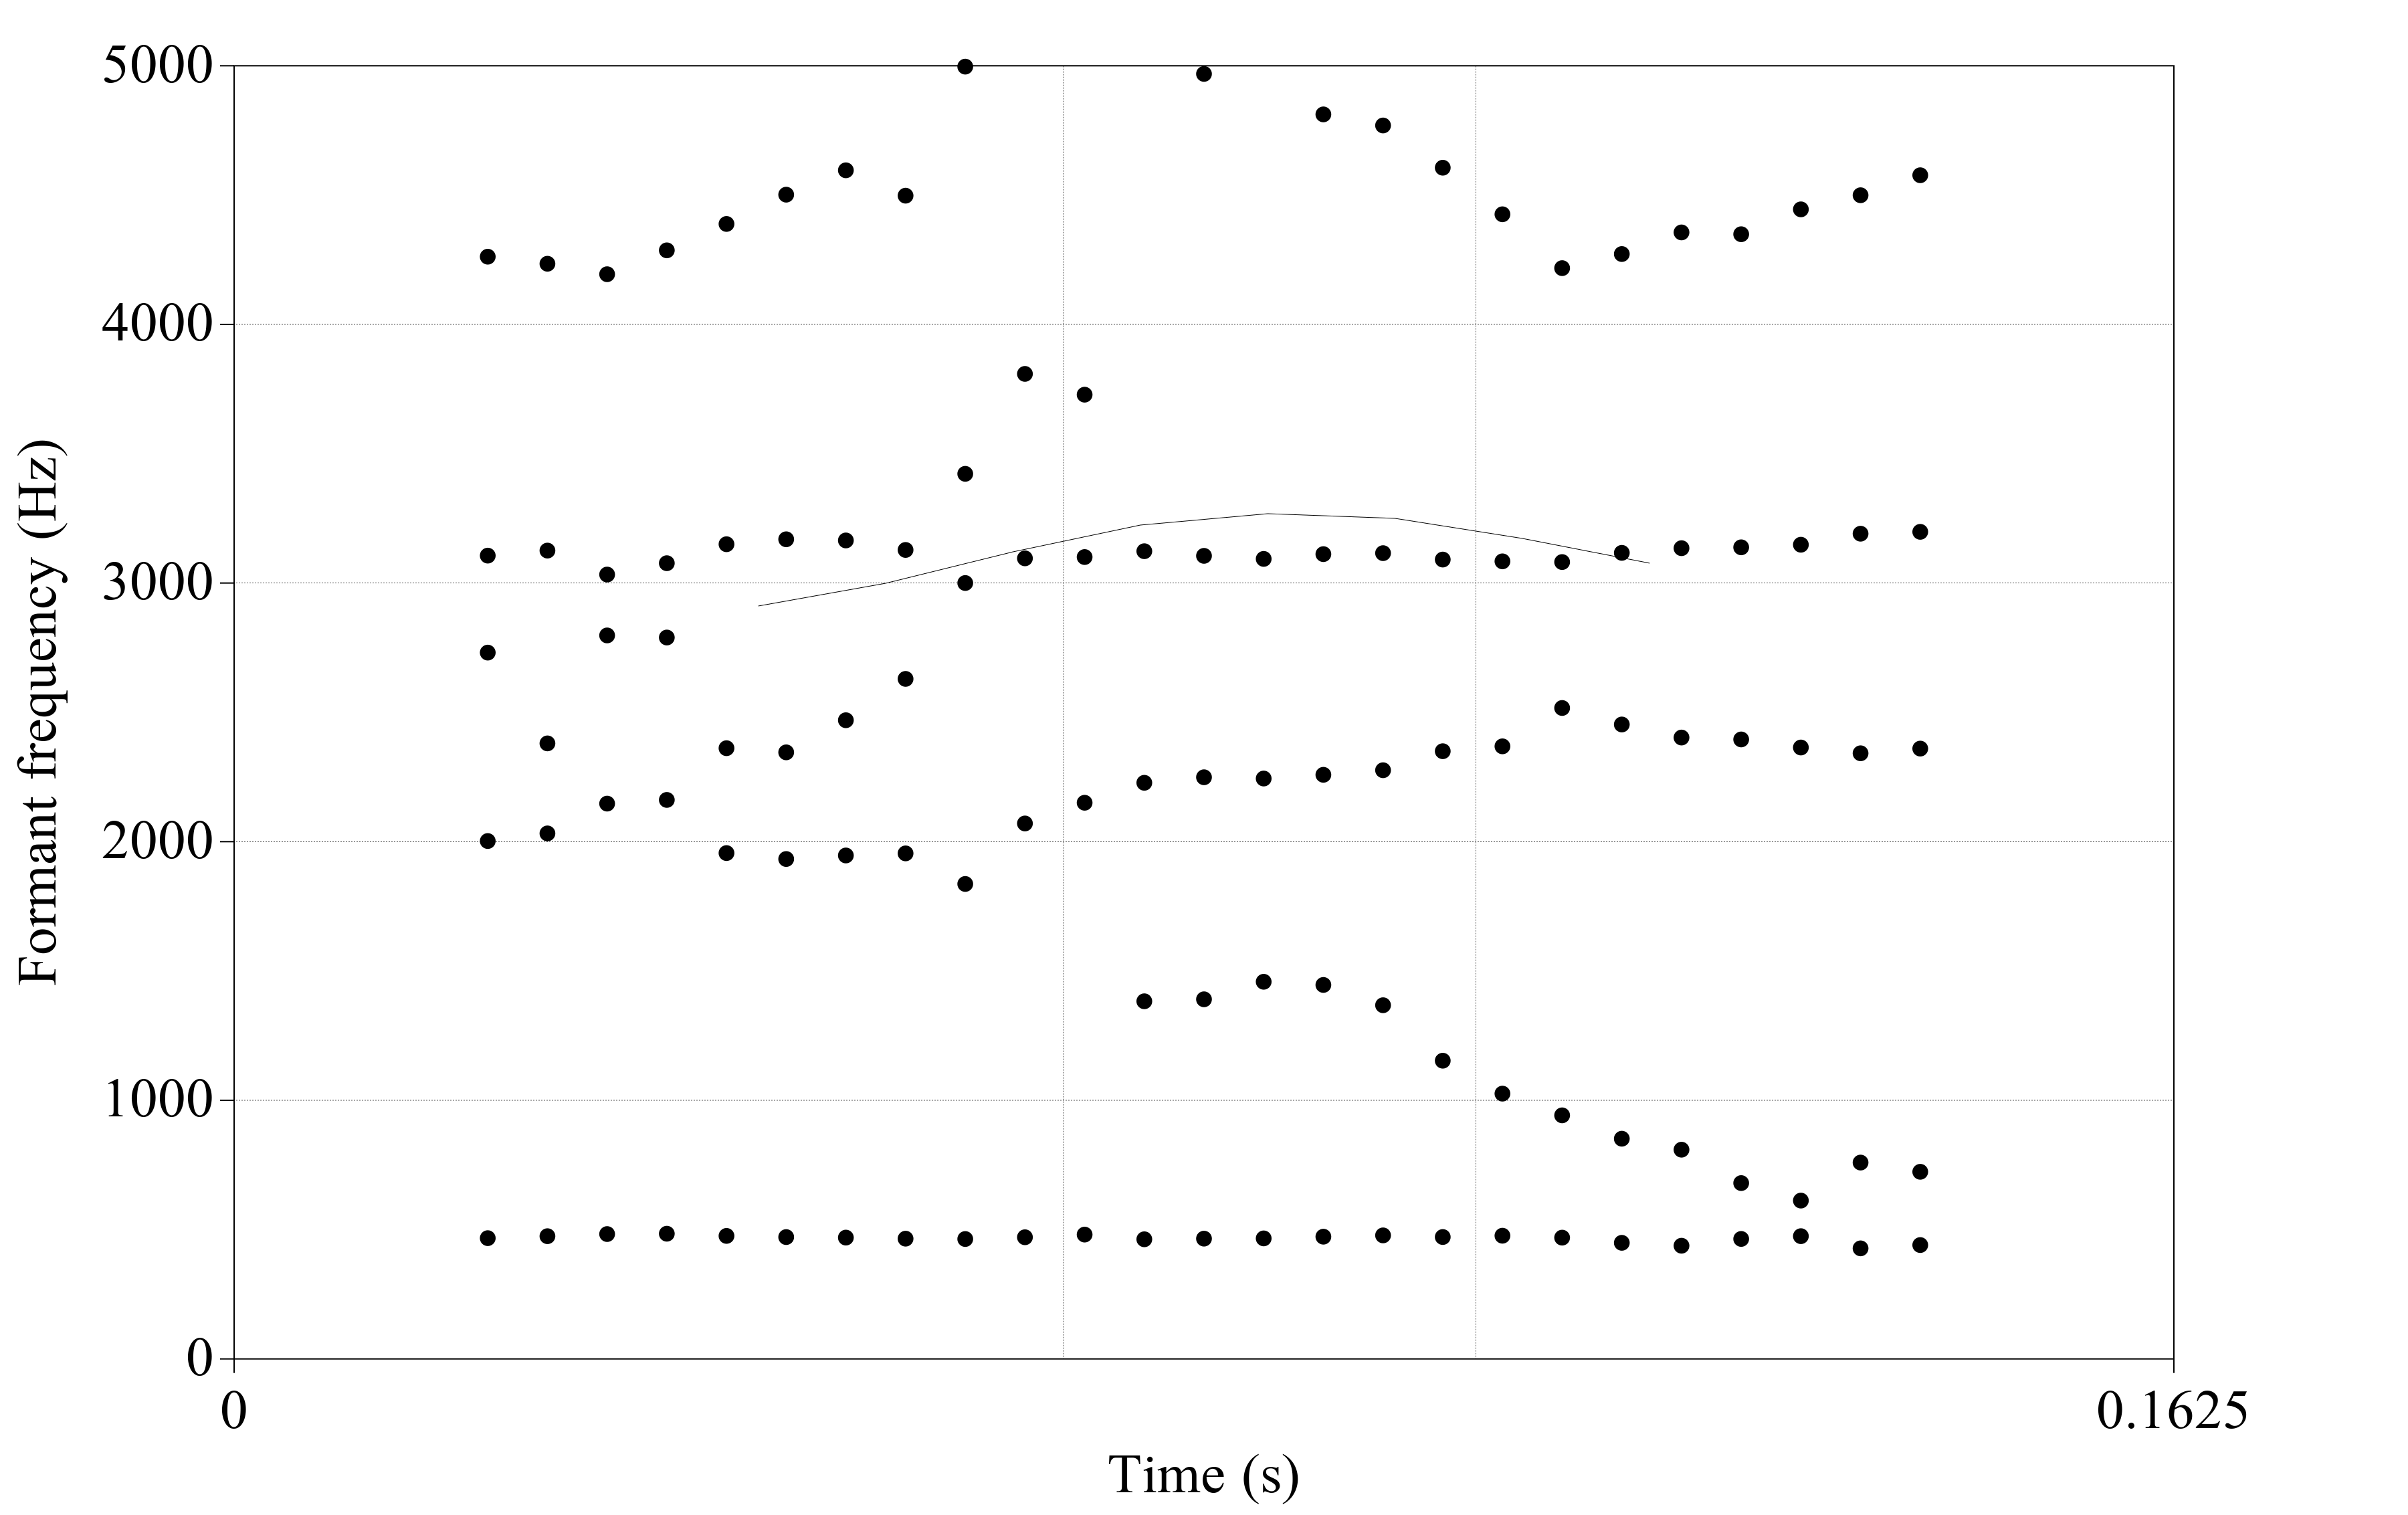
\includegraphics[height = 9.7cm]{images/eu.png}
	\caption{Diptongo /eu/.}
	\label{fig:eu}
\end{figure}

Más allá de los límites de la palabra, la métrica demanda una nueva incursión en el terreno de la fonética porque el diptongo es un mecanismo de ajuste silábico que se da de manera constante en los versos en la unión entre dos palabras cuando la primera acaba en una vocal y la siguiente empieza también con otra. En este caso, una de las dos vocales pierde su calidad vocálica al unirse a la otra. Hablamos aquí de una sinalefa\index{sinalefa}, y el accidente requiere la reevaluación del verso entero, en tanto que afecta al cómputo silábico, como veremos un poco más en detalle más adelante.

Desde una perspectiva acústica, estas propiedades son observables y cuantificables. De acuerdo con \citeauthor{milner2021}~\parencite*{milner2021}, las vocales\index{vocal} puras y los vocoides\index{vocoide} del español presentan diferencias acústicas en su primera y segunda frecuencia fundamental, que son más bajas en las vocales puras. De esta manera, el F2 de \ipa{[i̯]} y \ipa{[u̯]} es más alto que el de \ipa{[i]} y \ipa{[u]}, respectivamente. Se da asimismo una transición entre formantes\index{formante} y amplitud  a lo largo del segmento, lo que acorta la duración del diptongo respecto al hiato. En caso de sinalefa en el verso, se observa de esta manera si el diptongo impropio se realiza como creciente o decreciente.

\begin{table}[!ht]
	\centering\small
	\begin{tabular}{rccccc}
		\toprule
		& \textbf{Tipo} & \textbf{Ejemplo} &\textbf{t. fonológica} & \textbf{t. fonética}\\
		\midrule
		1&/iai/  &	\textit{estudiáis}	&	/estuˈdiais/	&	[estuˈðjai̯s]\\
		2&/iei/  &	\textit{vieira}		&       /ˈvieiɾa/	&	[estuˈðjei̯s]\\
		3&/ioi/  &	\textit{hioides}	&       /ˈioides/	&	[ˈjoi̯ðes]\\
		4&/iau/  &	\textit{«riau»}       &       /riau/		&	[rjau̯]\\
		5&/uai/  &	\textit{averiguáis}       &       /abeɾiˈguais/	&	[abeɾiˈɣwai̯s]\\
		6&/uei/  &	\textit{santigüéis}       &       /santiˈgueis/		&	[santiˈɣwei̯s]\\
		7&/uau/  & 	\textit{guau}       &       /guau/		&	[wau̯]\\
		\bottomrule
	\end{tabular}
	\caption{Triptongos.}
	\label{tab:triptongos
	}
\end{table}


Los triptongos\index{triptongo} son más escasos, y surgen de la combinación de un diptongo creciente y otro decreciente. En español solo hay siete tipos \parencite{canellada1987}. El resultado es un núcleo vocálico precedido de un sonido semiconsonántico y seguido de uno semivocálico. Este núcleo solo lo constituyen los fonemas \ipa{/a/}, \ipa{/e/} y \ipa{/o/}. Los sonidos no vocálicos los forman los fonemas \ipa{/i/} y \ipa{/u/}, con la particularidad de que no se dan las combinaciones \ipa{/ieu/}, \ipa{/iou/}, \ipa{/uoi/}, \ipa{/ueu/} y \ipa{/uou/}. Dicho de otra manera, las siete combinaciones fonéticas posibles son: \ipa{[jai̯]}, \ipa{[jei̯]}, \ipa{[joi̯]}, \ipa{[jau̯]}, \ipa{[wai̯]}, \ipa{[wei̯]} y \ipa{[wau̯]}.

Así pues, la fonología no resulta suficiente por sí misma para caracterizar la sílaba métrica en las uniones vocálicas. Para conocer su naturaleza, es necesario identificar el núcleo y, en caso de secuencia vocálica, localizar qué fonema es el preponderante, ya que los otros son irrelevantes en estas circunstancias.

\subsection{Sonidos consonánticos}\index{consonante}
Aunque no de tanta importancia como las vocales, ya que no afectan a la cuenta silábica, las consonantes desempeñan también un papel esencial. En primer lugar, la consonancia de la rima versal depende de ellas. En segundo, las reglas de división silábica las tienen en cuenta, por lo que su caracterización es necesaria a para deslindar sílabas. Sus propiedades físicas, por otra parte, interesan aquí en tanto que las distinguen de las vocales; las posibles realizaciones alternativas (p.ej. \textipa{/tRans.atˈlan.ti.ko/}, \textipa{/tRan.satˈlan'ti.ko/} o incluso la realización americana \textipa{/tRan.saˈtlan.ti.ko/}) se resuelven mediante reglas, que asumiremos sin entrar en otras discusiones que sobrepasarían el ámbito de este trabajo. Dejamos la puerta abierta a diferentes alternativas en la formalización de estos presupuestos teóricos para adaptar el análisis a un habla particular.

El repertorio del español dispone de tres fonemas oclusivos\index{consonante!oclusiva} sordos con oposición por el punto de articulación. El labial \ipa{/p/}, el dental \ipa{/t/} y el velar \ipa{/k/} \parencite[194-195]{quilis2019}.  De estos fonemas, \ipa{/t/} y \ipa{/d/} tienen realización laminar (predorsal) y \ipa{[t̪]} y \ipa{[d̪]} dentoalveolar \parencite[257]{martinez2003}. A los fonemas sordos se oponen respectivamente los sonoros \ipa{/b/}, \ipa{/d/} y \ipa{/g/}. No obstante, hay que hacer notar que el rasgo oclusivo no es pertinente en las últimas, ya que se realizan por norma general con los alófonos aproximantes \ipa{[β̞]}, \ipa{[ð̞]} y \ipa{[ɣ̞]} \parencite[79-132]{navarrotomas2004}. La realización oclusiva ocurre después de una consonante nasal o de pausa. Asimismo, en el caso de \ipa{/d/}, también se da el alófono oclusivo después de una consonante lateral. Los fonemas \ipa{/k/} y \ipa{/g/} son pospalatales cuando anteceden a \ipa{/i/} o \ipa{/e/}, por lo que su realización es \ipa{[k̞]} y \ipa{[g̞]} o \ipa{[ɣ̞]} \parencite[20-21]{canellada1987}.

Las oposiciones por sonoridad no son pertinentes en posición posnuclear, por lo que la oposición \ipa{/p/}-\ipa{/b/} se neutraliza a /B/ con rasgo común de labialidad, \ipa{/t/}-\ipa{/d/} a /D/ con rasgo común de dentalidad y \ipa{/k/}-\ipa{/g/} a /G/ con rasgo común de velaridad \parencite[205]{quilis2019}.
 
En cuanto a las consonantes nasales\index{consonante!nasal}, todos los fonemas de este tipo en el repertorio español son sonoros. Quilis describe tres fonemas: uno bilabial \ipa{/m/}, otro lingualveolar \ipa{/n/} y uno linguopalatal \ipa{/ɲ/}, que se oponen en posición silábica  prenuclear con una sola realización \ipa{[m]}, \ipa{[n]} y \ipa{[ɲ]} respectivamente \parencite[225]{quilis2019} y se neutralizan en el archifonema\index{archifonema} /N/ en coda. No obstante, \citeauthor{clegg2018}~\parencite*[331-337]{clegg2018} añaden a las realizaciones descritas por Quilis para /m/ la realización alternativa \ipa{[ɱ]} ante una consonante labiodental y para \ipa{/n/}, \ipa{[n̠]} ante un sonido interdental \ipa{[n̪]} ante uno dental, y las palatalizaciones \ipa{[n̠]} ante un sonido palatal y \ipa{[ŋ]} ante uno velar.

\begin{table}[h!]
	\centering\scriptsize
	\begin{tabular}{lcccccccc}
		\toprule	
		\multirow{3}{*}{\shortstack{\textbf{Modo}\\\textbf{de}\\\textbf{articulación}}} & \multicolumn{8}{c}{\textbf{Punto de articulación}} \\
		\cmidrule(lr){2-9}
		& \multicolumn{2}{c}{\textbf{Labial}} & \multicolumn{3}{c}{\textbf{Dental}} & \multirow{2}{*}{\textbf{Palat.}} &  \multicolumn{2}{c}{\textbf{Velar}} \\
		\cmidrule(lr){2-3}\cmidrule(lr){4-6}\cmidrule(lr){8-9}
		& \textbf{Bil.}&\textbf{L.-den.}&\textbf{Den.}&\textbf{Interd.}&\textbf{Alv.}&&\textbf{Vel.}&\textbf{Bil.-alv.}\\
		\midrule
		\textbf{Oclusiva}       &p \quad b&   &t \quad d&   & &   &k \quad g&  \\
		\textbf{Nasal}          &\quad \quad m&\quad \quad [ɱ]&\quad \quad [n̪]&\quad \quad [n̟]&\quad \quad n&\quad \quad ɲ&\quad \quad [ŋ]&  \\
		\textbf{Africada}       &   &   &   &   &   &t͡ʃ\quad[d͡ʒ]&   &  \\
		\textbf{Fricativa}      &   &f \quad \quad& &θ \quad \quad&s\quad\quad&     &x \quad \quad& \\
		\textbf{Aproximante}    &\quad \quad [β̞] &   & &\quad \quad [ð̞]&   &\quad \quad  ʝ [j]&\quad \quad [ɣ̞]&\quad \quad [w]\\
		\textbf{Lateral}        &   &   &\quad \quad [l̪]&\quad \quad [l̟]&\quad \quad l&\quad \quad ʎ&     & \\
		\textbf{Vibrante múlt.} &     &   &   &   &\quad \quad r&      & & \\
		\textbf{Vibrante simp.} &     &   &   &  &\quad \quad ɾ&       & & \\
		\bottomrule
	\end{tabular}
	\caption{Fonemas y alófonos consonánticos del español.}
	\label{tab:consonantes}
\end{table}


Cuando estos tres fonemas están en distensión silábica y preceden a una consonante, incluso entre palabras, su punto de articulación se asimila al de la consonante siguiente. De esta manera, por ejemplo, si la consonante nasal va seguida de una labial, se articula en posición labial (\textlangle{}invento\textrangle{} \ipa{/inˈbento/} \ipa{[imˈbento]}). En tal posición, el punto de articulación deja de ser pertinente y todas las nasales se neutralizan al archifonema /N/ (\ipa{/i\*Nˈbento/}). Este mismo fenómeno sucede en posición final absoluta \parencite[180-182]{alarcos1964}. Estos rasgos han de darse necesariamente porque la neutralización solo se da en fonemas muy cercanos \parencite[228-231]{quilis2019}. Martínez Celdrán \parencite*[51]{martinezceldran2004} hace notar al respecto que \ipa{/ɲ/} no debería considerarse salvo desde una perspectiva diacrónica porque solo se da en posición inicial en español moderno.

El español dispone de cuatro fonemas fricativos\index{consonante!fricativa} \ipa{/f/}, \ipa{/θ/}, \ipa{/s/} y \ipa{/x/} y uno africado\index{consonante!africada} \ipa{/\texttoptiebar{tʃ}/}, así como un sonido aproximante sonoro /ʝ/. Debemos añadir a estos los alófonos aproximantes de /b/, /d/ y /g/ arriba mencionados. Esta colección se refiere al español estándar, pues existen dialectos en los que no se da la oposición entre los fonemas /θ/ y /s/, por lo que optan por /s̄/ en todos los casos, lo que se conoce como \textit{ceceo}\index{ceceo} o por /s/, en cuyo caso hablamos de \textit{seseo}\index{seseo} \parencite[286]{clegg2018}.

El fonema /f/ es labiodental sordo y su realización normal es \ipa{[f]}, que se produce al obstruir el paso del aire colocando los incisivos sobre el labio inferior. Podemos decir que tiene una distribución única con el alófono \ipa{[f]} \parencite[246]{quilis2019}. El fonema  \ipa{/θ/} es interdental o linguinterdental, con el ápice lingual colocado sobre los incisivos \parencite[247]{quilis2019}. Ambos fonemas se sonorizarían ante consonante sonora como \ipa{[v]} y \ipa{[ð]}, respectivamente, aunque, el caso de \ipa{/f/} es muy raro por la escasez de casos de este fonema en posición de coda.

El fonema \ipa{/s/} tiene varias realizaciones para distintos dialectos. En Castilla, la realización es apicoalveolar \parencite[248]{quilis2019}. Este fonema se sonoriza habitualmente ante una consonante sonora y su realización es \ipa{[s̬]} \parencites{torreblanca1978}[251]{quilis2019}, pero puede no ser el caso, especialmente si el hablante  es una mujer \parencite{muniz2012}. Llama la atención que Quilis~\parencite*[251]{quilis2019} indique que el fonema /s/ suele perderse ante \ipa{/r/}, por lo que \textlangle{}dos reales\textrangle{} se pronunciaría \ipa{[ˈdo reˈales]} y, en una pronunciación muy cuidada, con una \ipa{/r/} asibilada [ˈdo ɹeˈales]. \citeauthor{navarrotomas2004}~\parencite*[107]{navarrotomas2004} no va tan lejos y, valiéndose de los mismos ejemplos, propone \ipa{[ˈdos̬ ɹeˈales]}, con una elisión total para casos muy particulares, al igual que hacen \citeauthor{canellada1987}~\parencite*[23]{canellada1987}.

El fonema \ipa{/ʝ/} tiene realización \textit{aproximante}\index{consonante!aproximante} en todos los contextos salvo después de pausa, nasal o lateral, en cuyo caso se presenta como una africada [\ipa{\texttoptiebar{ɟ\textlowering{ʝ}}}] \parencite{martinez2003}. No debe confundirse con el alófono \ipa{[j]} de \ipa{/i/}, que muestra diferencias acústicas y articulatorias significativas. Según \citeauthor{martinezceldran2004}~\parencite*[205-208]{martinezceldran2004}, estas se resumen en que \ipa{[j]} es más breve y con cierta frecuencia apenas un sonido de transición que solo existe acompañado de una vocal nuclear y no se da en ataque sino siempre en posición nuclear, mientras que el sonido \ipa{[\textlowering{ʝ}]} tiene una amplitud menor, de forma especial en $F_{2}$, y solo se da en ataque. A las características de este alófono habría que añadir la explosión con la que comienza el africado \ipa{[\texttoptiebar{ɟ\textlowering{ʝ}}]}. Tampoco debe confundirse con el sonido lateral \ipa{/ʎ/} \parencite[287]{clegg2018}, presente en el habla cuidada.

El fonema /x/ es velar en el español de Castilla, con un alófono \ipa{[χ]} antes de \ipa{/o/} y \ipa{/u/} en todas sus realizaciones \parencite{martinez2003}. Por su parte, el africado \ipa{/\texttoptiebar{tʃ}/} es linguopalatal sordo.

En lo que respecta a las \textit{consonantes líquidas}\index{consonante!líquida}, encontramos dos laterales con sus respectivos alófonos y dos vibrantes, una simple y otra múltiple. Las laterales\index{consonante!lateral} en español son \ipa{/l/} y \ipa{/ʎ/}, aunque esta última está en vías de desaparición y predomina únicamente en las variedades septentrionales ibéricas y en las tierras altas americanas, siendo lo habitual en el sur de España y América que se neutralice a /ʝ/. Las laterales se caracterizan por presentar formantes\index{formante} atenuados debido al cierre central, que, junto a las transiciones vocálicas —menos abruptas, en cualquier caso, que para las consonantes nasales—, indican el lugar de articulación.

El fonema /l/ es lateral lingualveolar y se realiza como \ipa{[l]}, salvo en algunas posiciones silábica posnucleares \parencite[309-310]{quilis2019}. Cuando precede a \textipa{/T/}, se desplaza hasta una posición interdental (\textlangle{}colza\textrangle{} \textipa{[ko\textsubplus{l}Ta]}), antes de \ipa{/t/} o \ipa{/d/} es linguodental (\textlangle{}caldo\textrangle{} \textipa{[ka\textsubbridge{l}do]}) y ante palatal se realiza linguopalatalizado (\textlangle{}el ñu\textrangle{} \textipa{[e\textsubbar{l} \textltailn u]}) \parencite[341-250]{clegg2018}. El fonema \ipa{/l/} se da en la posición inmediatamente anterior o posterior al núcleo vocálico, mientras que \textipa{/ʎ/} solo aparece en posición prenuclear en palabras patrimoniales. Esto hace cuestionable una neutralización a /L/ de las laterales desde una perspectiva sincrónica.

En castellano encontramos una consonante vibrante\index{consonante!vibrante} simple\index{consonante!vibrante!simple} \textipa{/R/} y una múltiple\index{consonante!vibrante!múltiple} \ipa{/r/}. Se producen colocando el ápice de la lengua contra los alvéolos para generar una o varias oclusiones. Ambas son apicoalveolares y no tienen más que un alófono. La vibrante simple solo aparece en interior de palabra en posición prenuclear entre vocales (\textlangle{}hora\textrangle{} \textipa{/ˈoRa/}) o entre \ipa{/p/}, \ipa{/t/}, \ipa{/k/}, \ipa{/b/}, \ipa{/d/}, \ipa{/g/} o \ipa{/f/} y vocal (\textlangle{}protráctil\textrangle{} \textipa{/pRoˈtRaktil/}, \textlangle{}crabrón\textrangle{} \textipa{/kRaˈbRon/} y \textlangle{}grecofrancés\textrangle{} \textipa{/gRekofRanˈTes/} ) \parencite[330]{quilis2019}. La oposición  entre \ipa{/r/} y \textipa{/R/}  solo es pertinente fonológicamente en posición intervocálica (\textlangle{}perro\textrangle{} \ipa{/pero/}-\textlangle{}pero\textrangle{} \textipa{/peRo/}), por lo que en todas las demás posiciones se neutraliza al archifonema /R/ \parencite{alarcos1964}.

Al contrario que con las vocales, la caracterización fina de las consonantes sí tiene consecuencias en el metro. Dicho de forma más precisa, la neutralización fonémica podría afectar a una parte tan importante como es la rima. Si bien resultaría difícil hallarlo, es una posibilidad teórica real. Por ejemplo, \textlangle{}Abraham\textrangle{} y \textlangle{}Guzmán\textrangle{} serían \textipa{/abraˈa}N/ y \textipa{/guTˈma}N/ y, por lo tanto, formarían rima consonante.

\section{División silábica del español}\label{sec:silabas}
\subsection{Características generales}
La sílaba española consiste en un núcleo vocálico obligatorio, opcionalmente precedido de un ataque o seguido de una coda, ambos consonánticos (\Cref{fig:silabeo}). El núcleo consta generalmente de una sola vocal como /o/ en \textlangle{}ocaso\textrangle{} \ipa{[o.ˈka.so]}, pero puede ir unido a vocales débiles en forma de vocoide\index{vocoide}, precedido de una semiconsonante como en \textlangle{}idiota\textrangle{} \ipa{[i.ˈðjo.ta]}\index{semiconsonante} o seguido de una semivocal\index{semivocal} como en \textlangle{}hoy\textrangle{} \ipa{[oi̯]}, lo que constituiría sendos diptongos, o incluso orlado a ambos lados, como en \textlangle{}dioico\textrangle{} \ipa{[ˈðjoi̯.ko]}, en cuyo caso hablaríamos de triptongo\index{triptongo}. Por su parte, tanto coda como ataque, cuando se dan, están compuestos por entre una y dos consonantes. Se denomina sílaba libre a aquella que consta de un núcleo vocálico en solitario o acompañado de uno o dos sonidos consonánticos en ataque, y trabada a la que tiene más de un sonido consonántico en coda \parencite[46-47]{navarrotomas1946}.

\begin{figure}[!ht]
	\centering
\begin{tikzpicture}
\tikzset{frontier/.style={distance from root=150pt}}
    \Tree   [.{\textbf{Palabra}} 
[.{\textbf{\upshape S$_1$}} 
[[.\textit{Ataque} [.C$_1$ {\textit{t}} ] 
[.C$_2$ {\textit{r}} ]]] 
[.\textit{Rima}
[.\textit{Núcleo} [.C$_1$ {\textit{a}} ] ]
[.\textit{Coda}  [.C$_2$ {\textit{n}} ] 
[.C$_2$ {\textit{s}} ] ] ] ]
%
%
[.{\textbf{\upshape S$_2$}} 
[[.\textit{Ataque} [.C$_1$ {\textit{p}} ]] ]
[.\textit{Rima}
[.\textit{Núcleo}  [.S$_1$ {\textit{u}} ]
[.V {\textit{e}} ] ]
[.\textit{Coda} [.C$_1$ {\textit{s}} ] ]]]
%
%
[.{\textbf{\upshape S$_3$}} 
[[.\textit{Ataque} [.C$_1$ {\textit{t}} ] ]]
[.\textit{Rima}
[.\textit{Núcleo}  [.V {\textit{o}} ] ]]]
]
\end{tikzpicture}

\caption{Construcción sílabas.}
\label{fig:silabeo}
\end{figure}

De acuerdo esto, tenemos nueve combinaciones posibles del núcleo con hasta dos consonantes en ataque o en coda, distribuidas según lo mostrado en el ejemplo \ref{ex:silabaaa}. 
\begin{exe}\ex\label{ex:silabaaa}
\begin{tabular}{ l l }
	V & \textit{y}, \textit{o},  \\ 
	CV & \textit{la}, \textit{de},  \\
	VC & \textit{un}, \textit{él}  \\ 
	CVC & \textit{mar}, \textit{ven}, \\ 
	CCV & \textit{\textbf{bra}·sa}, \textit{la·\textbf{cre}}  \\
	VCC & \textit{\textbf{obs}·ce·no},  \textit{\textbf{ins}·pi·ra·ción} \\
	CCVC & \textit{\textbf{bron}·ce}, \textit{im-\textbf{pren}·ta} \\ 
	CVCC & \textit{\textbf{pers}·pec·ti·va}, \textit{\textbf{cons}·cien·te}  \\ 
	CCVCC & \textit{\textbf{trans}·mu·tar}
\end{tabular}
\end{exe}
Cualquier consonante puede ocupar la posición de ataque en solitario. Sin embargo, si hay dos consonantes, no todas las combinaciones son posibles. En posición de coda ocurre lo mismo, con la restricción adicional de que determinadas consonantes no se dan jamás en dicha posición.

Asimismo, aparece como máximo una sola consonante a final de palabra en español moderno, al contrario que en otras variedades diacrónicas donde se dan casos como \textit{puent}, \textit{muert} \parencite[49]{navarrotomas1946}. No obstante, las pocas coincidencias relativamente recientes que se encuentran en el CORDE  nos remiten a documentos de la primera mitad del siglo \textsc{xvi}, por lo que, considerando asimismo que el registro escrito es más conservador que la lengua hablada, asumimos que el español del Siglo de Oro se comporta en este sentido como la variedad moderna.

\subsection{División entre vocales}\label{sec:irregularidades}
En la división vocálica podemos distinguir los casos vocal\textsuperscript{$+\textsc{alta}$} vocal\textsuperscript{$+\textsc{alta}$}, vocal\textsuperscript{$+\textsc{alta}$} vocal\textsuperscript{$-\textsc{alta}$}, vocal\textsuperscript{$-\textsc{alta}$} vocal\textsuperscript{$+\textsc{alta}$} y vocal\textsuperscript{$-\textsc{alta}$} vocal\textsuperscript{$-\textsc{alta}$}. Exclusivamente el último de los cuatro casos forma siempre un hiato. Todos los otros casos constituyen diptongo o hiato \parencite{riosmestre1999}. De esta forma, \textlangle{}crear\textrangle{} será necesariamente bisilábica \textipa{/kReˈaR/}, pero tenemos \textlangle{}lío\textrangle{} \textipa{/ˈli.o/} \ipa{[ˈli.o]},
\textlangle{}lio\textrangle{} \textipa{/liˈo/} \ipa{[liˈo]} o \textlangle{}vio\textrangle{} \ipa{/bio/} \ipa{[Bjo]} 
y \textlangle{}voy\textrangle{} \textipa{/ai/} \ipa{[ai̯]} o \textlangle{}ahí\textrangle{} \ipa{/a.ˈi/} \ipa{[a.ˈi]}, y \textlangle{}fui\textrangle{} \ipa{/fui/} \ipa{[fwi]} o \textlangle{}hui\textrangle{} \ipa{/u.ˈi/} \ipa{[/u.ˈi/]}. Aunque la división silábica se infiere de la ortografía la mayoría de las veces, este no es siempre el caso, como vemos, por ejemplo, en \textlangle{}criado\textrangle{} \textipa{/kRi.ˈa.do/} \textipa{[kRi.ˈa.ðo]} y \textlangle{}aciago\textrangle{} \textipa{/a.ˈTia.go/} \textipa{[a.ˈTja.Go]}.

De acuerdo con \citeauthor{quilis2019}~\parencite*[184-186]{quilis2019}, dos vocales átonas forman diptongo si al menos una de ellas es alta. La secuencia vocal\textsuperscript{$+\textsc{alta}$} vocal\textsuperscript{$-\textsc{alta}$} o vocal\textsuperscript{$-\textsc{alta}$} vocal\textsuperscript{$+\textsc{alta}$} forma diptongo cuando la vocal alta es tónica. El resto de los casos suele formar diptongo, salvo en los siguientes casos descritos por el autor:

\paragraph{Verbos en \textit{-iar}:}{\textit{agriar}, \textit{aliar}, \textit{ampliar}, \textit{arriar}, \textit{ataviar}, \textit{autoviar}, \textit{aviar}, \textit{ciar}, \textit{confiar}, \textit{congloriar}, \textit{contrariar}, \textit{criar}, \textit{desafiar}, \textit{desaviar}, \textit{descarriar}, \textit{desconfiar}, \textit{desvariar}, \textit{desviar}, \textit{enfriar}, \textit{enviar}, \textit{espiar}, \textit{estriar}, \textit{expiar},  \textit{extraviar}, \textit{ferroviar}, \textit{fiar}, \textit{gloriar}, \textit{grafiar}, \textit{guiar}, \textit{hastiar}, \textit{istriar}, \textit{liar}, \textit{malcriar}, \textit{piar}, \textit{porfiar}, \textit{recriar}, \textit{reenviar}, \textit{resfriar}, \textit{triar} y \textit{vaciar}. Previene, no obstante, que no afecta el futuro y al condicional porque, mientras que en \textit{fiar}, \textit{fía} o \textit{fio} una de las vocales es tónica, en \textit{fiaré} o \textit{fiaría} son ambas átonas.}

\paragraph{Verbos en \textit{-uar}:}{\textit{acentuar}, \textit{actuar}, \textit{atenuar}, \textit{cansuar}, \textit{conceptuar}, \textit{contextuar}, \textit{continuar}, \textit{descontinuar}, \textit{desgraduar}, \textit{deshabituar}, \textit{desvirtuar}, \textit{estatuar}, \textit{evaluar}, \textit{exceptuar}, \textit{extenuar}, \textit{fluctuar}, \textit{ganzuar}, \textit{graduar}, \textit{habituar}, \textit{individuar}, \textit{infatuar}, \textit{insinuar}, \textit{menstruar}, \textit{perceptuar}, \textit{perpetuar}, \textit{puar}, \textit{puntuar}, \textit{ruar}, \textit{situar}, \textit{tatuar}, \textit{tumultuar},  \textit{usufructuar} y \textit{valuar}, y se exceptúan los verbos terminados en \textit{-cuar} \textipa{[kwaR]} y \textit{-guar} \textipa{[gwaR]}, que forman diptongo en todos los casos y, por el mismo motivo que los verbos en \textit{-iar}, el futuro y el condicional.}
	
\paragraph{Verbos en \textit{-uir}:}{\textit{afluir}, \textit{argüir}, \textit{atribuir}, \textit{circuir}, \textit{concluir}, \textit{constituir}, \textit{construir}, \textit{contribuir}, \textit{derruir}, \textit{destituir}, \textit{destruir}, \textit{diluir}, \textit{disminuir}, \textit{distribuir}, \textit{esmuir}, \textit{estatuir}, \textit{excluir}, \textit{fluir}, \textit{huir}, \textit{imbuir}, \textit{incluir}, \textit{influir}, \textit{inmiscuir}, \textit{instituir}, \textit{instruir}, \textit{intuir}, \textit{irruir}, \textit{muir}, \textit{obstruir}, \textit{ocluir}, \textit{prostituir}, \textit{recluir}, \textit{reconstituir}, \textit{reconstruir}, \textit{redargüir}, \textit{refluir}, \textit{rehuir}, \textit{restituir}, \textit{retribuir} y \textit{sustituir}. La excepción del condicional y el futuro aplica aquí también.}

\paragraph{Adjetivos en \textit{-uoso(s)}/\textit{-uosa(s)}:}{\textit{suntuoso}, \textit{virtuoso}, \textit{sinuoso}}.

\paragraph{Casos particulares y sus flexiones:}{\textit{acuoso}, \textit{anual},  \textit{arriero}, \textit{bienio}, \textit{biombo}, \textit{boquiancho}, \textit{cliente}, \textit{crianza}, \textit{cruel}, \textit{desconfianza}, \textit{diablo}, \textit{diálogo}, \textit{dieciocho}, \textit{ferrovial}, \textit{fianza}, \textit{gorrión}, \textit{guión}, \textit{hiato}, \textit{maniobra}, \textit{miasma}, \textit{piano}, \textit{prior}, \textit{santuario}, \textit{Sión}, \textit{tiara}, \textit{triángulo}, \textit{trienio}, \textit{truhán} y \textit{ventiocho}. Navarro~Tomás~\parencite*[68]{navarrotomas2004} añade \textit{ruido}, \textit{suave}, \textit{viaje} y \textit{viuda}.}

\paragraph{Secuencias /ˈi.u/, /ˈu.i/, /iˈu/ o /uˈi/:}{\textit{jesuita}, \textit{circuito}, \textit{fortuito}, \textit{casuística} y \textit{diurno}.}

A esto debemos añadir los verbos en \textit{-eír} \parencite[6.8.2.1.2.2]{riosmestre1999}, como \textit{desleír}, \textit{engreír}, \textit{freír}, \textit{refreír}, \textit{reír}, \textit{sofreír} y \textit{sonreír}. Se volvería a excluir el futuro y el condicional. \citeauthor{riosmestre1999}~\parencite*[6.8.2.1.2.3]{riosmestre1999} alude asimismo a los verbos en \textit{-oír}, pues considera inoportunas las salvedades del futuro y el condicional. 

\citeauthor{canellada1987}~\parencite*[51-52]{canellada1987} señalan asimismo \textit{ahilarse}, \textit{baulero}, \textit{buhonero}, \textit{criador}, \textit{huidizo}, \textit{miopía}, \textit{prohibir}, \textit{reunión}, \textit{reiré} y \textit{semiesfera}. Observamos que estos son bien derivados de palabras sin ambigüedad ortográfica, de las excepciones descritas o resultado de la prefijación, a excepción de \textit{buhonero}, \textit{miopía} y \textit{prohibir}.

No hemos considerado prefijos acabados en vocal como \textit{re-} o \textit{tri-} (por ejemplo, \textit{rehilamiento} y \textit{triángulo}), que podrían tender a formar hiato en algunas circunstancias, como un habla muy lenta, dado que la literatura al respecto ha resultado ser muy escasa. Sin embargo, incluimos un archivo de excepciones en la formalización donde forzar el hiato en casos particulares para modificar el comportamiento del módulo que realiza la silabación. Las entradas correspondientes llevan una marca que las identifica como comentarios y no como reglas, por lo que no se tienen en cuenta; esta marca se borra discrecionalmente cuando se desea hacer el hiato.

\subsection{División entre consonantes}
Podemos distinguir los siguientes casos: una consonante intervocálica, grupo de dos consonantes intervocálicas, tres o más consonantes intervocálicas, que Quilis~\parencite*[367-369]{quilis2019} resuelve de tres maneras diferentes.

\paragraph{V-C-C-V:}{El caso más simple es el de una consonante intervocálica. Dado que el español tiene tendencia a las sílabas abiertas, dicha consonante se agrupará con la sílaba siguiente.}


\paragraph{V-C-C-V:}{Si las consonantes son una agrupación de consonante del tipo \textit{muta cum liquida}, esto es bilabial o labiodental (/p/, /b/, /f/) o linguovelar (/g/, /k/) seguida de una líquida (\textipa{/R/}, /l/) o una linguodental(/d/, /t/) seguida de vibrante (\textipa{/R/}), nos encontramos ante una unidad inseparable que forma la coda del núcleo silábico siguiente (\textit{probar}, \textit{plomo}, \textit{broma}, \textit{blanco}, \textit{francés}, \textit{flanco},\textit{gracia}, \textit{glosa}, \textit{craso},  \textit{claro},  \textit{drama},  \textit{trama}). Cualquier otra combinación se reparte entre la primera y la segunda sílaba.}

\paragraph{V-C-C-C-(C)-V:}{Para que se dé una combinación de tres consonantes, los dos últimos fonemas deben formar una unidad inseparable como las descritas en el párrafo anterior o bien las dos primeras deben ser una agrupación del tipo /Ns/ o /Bs/ (\textlangle{}constar\textrangle{} \textipa{/konsˈtaR/}, \textlangle{}obstar\textrangle{} \textipa{/obsˈtaR/}). Si hay cuatro consonantes seguidas se trata de una conjunción de ambos casos (\textlangle{}abstracción\textrangle{} \textipa{/abs.tRakˈTion/}), por lo que se reparten dos en cada núcleo.}

\subsection{Contacto entre vocales de diferentes palabras}
El principio fundamental de la reducción vocálica a grupos silábicos reza que, según la fonética, dos vocales cualesquiera en contacto admiten reducirse siempre a una sola sílaba, por lo que lo harán si no hay razones gramaticales o de otra índole que lo impidan \parencite[136]{navarrotomas2004}. \citeauthor{canellada1987}~\parencite*[55]{canellada1987} hacen una descripción detallada de las circunstancias que concurren en los límites de palabra cuando hay dos vocales en contacto y cómo se resuelven estas uniones. Según los autores, se producen cuatro tipos de unión: \textit{hiato}\index{hiato}, \textit{reducción}\index{reducción}, \textit{diptongación}\index{diptongo} y \textit{elisión}\index{elisión}. Salvo en el hiato, hablaremos en estos casos de \textit{sinalefa}. Llamamos sinalefa\index{sinalefa} a la unión en una única sílaba de dos vocales adyacentes ubicadas en posición final e inicial de sendas palabras contiguas. Pueden unirse de esta manera hasta cinco vocales distribuidas a lo largo de hasta tres palabras, como, por ejemplo, en \textlangle{}repudio a Eugenia\textrangle{} \ipa{[reˈpu.djo̯ae̯u̯ˈxe.nja]}. Para que ocurra una sinalefa han de cumplirse cuatro condiciones:
\begin{enumerate}
	\item La pronunciación debe ser rápida.
	\item No hay enfatizaciones.
	\item Si intervienen más de dos vocales, entre dos vocales abiertas solamente puede haber otra abierta.
\end{enumerate}

Si no se cumplen estas condiciones, lo normal es que se produzca un hiato \textipa{/boi̯.aˈka.sa/} o, si acaso, que se redistribuyan las fronteras silábicas \textipa{/bo.Jaˈka.sa/}. Cuando sí concurren todas las condiciones necesarias, la resolución de la sinalefa varía en función de las partes que la constituyen. 

De esta manera, si  se encuentran dos vocales iguales, estas se funden en una. Si el resultado tiene más cantidad, hablaríamos de reducción\index{reducción} (\ref{ex:red}). Por el contrario, si la cantidad es regular, hablaremos de elisión\index{elisión} (\ref{ex:eli}). La realización según uno u otro recurso depende sobre todo de la velocidad de la pronunciación. Además, si una de las vocales es tónica, la unión también será tónica \parencite[138-139]{navarrotomas2004}.
\begin{exe}
\ex\textlangle{}va a verlo\textrangle{}\begin{xlist}
\ex{\textipa{/ˈba:ˈbeR.lo/}}\label{ex:red}
\ex{\textipa{/ˈbaˈbeR.lo/}}\label{ex:eli}	
\end{xlist}
\end{exe}

Si las vocales son diferentes, una de las dos pierde su condición silábica, pero conservar el timbre vocálico. En este caso, se trataría de una reducción  (\ref{ex:red1}). Cuál de ambas vocales hace de núcleo y cuál se reduce depende de varios factores. Si ambas son átonas, el elemento de la segunda posición tiene precedencia (\ref{ex:red2}). Si una de las dos partes es tónica y la otra no, se prefiere la vocal tónica para hacer de núcleo (\ref{ex:red3}). En cualquier otro caso, la vocal más abierta precede a la más cerrada como posible núcleo (\ref{ex:red4}) \parencite[140-152]{navarrotomas2004}.
\begin{exe}
	\ex\label{ex:red1}\textlangle{}se acerca\textrangle{} \textipa{/se̯aˈTeR.ka/}
		\ex\label{ex:red2}\textlangle{}parece huraño\textrangle{} \textipa{/paˈRe.Te̯uˈRa.No/}
		\ex\label{ex:red3}\textlangle{}la hebra\textrangle{} \textipa{/ˈla̯e.bRa/}/
		\ex\label{ex:red4}\textlangle{}va este\textrangle{} \textipa{/ˈbae̯s.te/}
\end{exe}
En el último caso, hay que tener además en cuenta la escala de perceptibilidad, que, según \citeauthor{navarrotomas2004}~\parencite*[25]{navarrotomas2004}, se establece según el grado de apertura bucal, por lo que /a/ sería la vocal más perceptible, seguida de /o/ y de /e/ y las menos perceptibles serían /i/ y /u/. Asimismo, al igual que ocurre entre vocales iguales, si una de las partes de la unión es tónica, la sílaba resultante también lo será \parencite*[142]{navarrotomas2004}.

Si la vocal que pierde su calidad de núcleo silábico es /i/ o /u/, también lo hace con su condición vocálica, de forma que \textlangle{}mi amigo\textrangle{} se pronunciaría \textipa{/mjaˈmi.go/} en ese caso. Además, si la vocal cerrada es tónica, el acento se desplaza a la siguiente vocal. Esto es, en \textlangle{}salí ayer\textrangle{} \textipa{/saˈljaˈJeR/}, el acento recaería en \ipa{[a]}. Esto se confirma también en la poesía \parencite{esgueva2004}.

La elisión total, aunque no es ajena a la lengua hablada —especialmente en expresiones hechas como \textit{*sabusté} o \textit{*sacabao}—, se considera propia de registros vulgares. En cualquier caso, dado que, en las representaciones dramáticas de las que nos ocupamos, el habla es intencionalmente cuidada —se declama—, esta situación no debería suponer un inconveniente. Podemos asumir que el dramaturgo habría indicado explícitamente si alguna pronunciación ha de ser deliberadamente inadecuada, como, por ejemplo, cuando un rústico habla sayagués. Aquí, claro está, se hace patente la necesidad de una buena edición que enmiende el exceso de celo corrector de algún cajista. 

Si la agrupación es de más de dos vocales, la reducción no es siempre posible. Para que esto suceda, deben estar agrupadas de menor a mayor perceptibilidad si la última vocal es nuclear (\ref{ex:menosmas}), y viceversa si es la primera (\ref{ex:masmenos}). Si la vocal nuclear ocupa una posición central, el grado de perceptibilidad de las vocales no nucleares debe reducirse en ambas direcciones  (\ref{ex:menosmasmenos}), de modo que, si la secuencia vocálica continúa, la vocal menos perceptible represente la división silábica.

\begin{exe}
	\ex\label{ex:menosmas}\textlangle{}espíritu o aliento\textrangle{} \textipa{/esˈpi.Ri.tu̯o̯aˈljen.to/}
	\ex\label{ex:masmenos}\textlangle{}halla o ubica\textrangle{} \textipa{/ˈa.Lao̯u̯ˈbi.ka/}
	\ex\label{ex:menosmasmenos}\textlangle{}vengo a esperar\textrangle{} \textipa{/ˈven.go̯ae̯s.peˈRaR/}
\end{exe}

Puede darse en este último caso la ambigüedad de que la vocal reducida liminar se agrupe indistintamente con el primer núcleo (\ref{ex:menosmasmenosmasa}) o con el segundo (\ref{ex:menosmasmenosmasb}).
\begin{exe}
	\ex\textlangle{}la he asado\textrangle{}
	\begin{xlist}
		\ex\label{ex:menosmasmenosmasa}\textipa{/ˈla̯e.aˈsa.do/}
		\ex\label{ex:menosmasmenosmasb}\textipa{/laˈe̯aˈsa.do/}
	\end{xlist}
\end{exe}

\subsection{Conjunciones \textit{y}/\textit{e} y \textit{o}/\textit{u}}\index{conjunción}\label{sec:conj}
La conjunción \textit{y} se une a las siguientes vocales observando unas normas \parencites[59]{canellada1987}[49]{navarrotomas2004}. Cuando aparece en posición interconsonántica, se pronuncia como \ipa{/i/} de relajación variable. Cuando va entre una consonante y una vocal, se realiza como semiconsonante en diptongo con el fonema vocálico siguiente y se pronuncia \ipa{/j/}, salvo que vaya precedida de \ipa{/s/} o \ipa{/z/}, en cuyo caso la pronunciación será consonántica y se unirá en ataque como \ipa{/ʝ/}. En la situación inversa, si va precedido de una vocal y seguido de una consonante, diptonga con el núcleo vocálico precedente en calidad de semivocal como \ipa{/i̯/}. La última posibilidad es que se encuentre entre dos vocales, en cuyo caso tendrá calidad consonántica y se unirá en ataque a la sílaba de su derecha como \ipa{/ʝ/}.

Las conjunciones \textit{e}, \textit{o} y \textit{u} suelen unirse con una consonante final de la primera palabra y diptongan con la vocal inicial de la segunda \parencite[60]{canellada1987}. Entre vocales, suele producirse un hiato con la primera palabra y un diptongo con la segunda tanto para \textit{e} como para \textit{o} \parencite[60]{canellada1987}. Lo mismo señala \citeauthor{bello1981}~\parencite*[109-111]{bello1981}, que llama la atención sobre lo áspera que se hace al oído castellano la ligadura de dos vocales por \textit{o}. No obstante, Bello indica que la conjunción \textit{e} funciona de manera opuesta, uniéndose a la vocal precedente. 
	
\section{Transcripción grafémico-fonológica}\label{transgraffon}
\citeauthor{riosmestre1999}~\parencite*[2.3]{riosmestre1999} describe tres procedimientos de transcripción: por reglas\index{transcripción!por reglas}, si se toma como entrada los grafemas\index{grafema} para transformarlos, por diccionario\index{transcripción!por diccionario}, si se toman unidades léxicas, y la pronunciación por analogía, basada en la inteligencia artificial. Los sistemas basados en reglas son los menos costosos de construir porque se fundamentan en la sistematización de la teoría lingüística. Estos se modifican de manera sencilla y la corrección de errores es rápida. Como contrapartida, son lentos, y su velocidad disminuye en función del número de reglas por lo que, a mayor precisión, mayor lentitud. La transcripción por diccionarios es más exacta además de veloz, pero, por su propia naturaleza, solo admite transcribir palabras previamente almacenadas. Independientemente de esto, decidirse por uno u otro método requiere, además, tener en cuenta otro aspecto fundamental: la relación entre grafema\index{grafema} y fonema\index{fonema} de la lengua en cuestión. 

El sistema de reglas se ha empleado tradicionalmente en la conversión de texto a habla, con buenos resultados \parencites{perez1991}{lopez1993}{rodriguez1998}, pero no siempre conduce a una resolución óptima de todos los casos si la ortografía no da lugar a la interpretación fonética libre de ambigüedad. En esos casos, las irregularidades demandan procedimientos específicos. Entre estos, señalaremos  la regularización de las excepciones ortográficas o las listas de palabras \parencite*[2.3]{riosmestre1999}. Esta última aproximación usaría la transcripción mediante diccionario como apoyo para la transcripción por reglas.

En cuanto a la formalización de las reglas, \citeauthor{riosmestre1999}~\parencite*[2.4]{riosmestre1999} se basa en \citeauthor{chomsky1968}~\parencite*{chomsky1968} para enunciar cuatro tipos de reglas de transformación. Primero, habría reglas biunívocas, cuando un grafema se transcribe con un único fonema, por ejemplo, \textlangle{}t\textrangle{} $\rightarrow$ /t/. El siguiente tipo sería la correspondencia dos a uno, en el caso de un dígrafo\index{dígrafo}, por ejemplo \textlangle{}qu\textrangle{} $\rightarrow$ /k/. También se da el caso contrario, con una correspondencia uno a dos, cuando a un grafema le corresponden dos fonemas, como en el caso de  \textlangle{}x\textrangle{} $\rightarrow$ /ks/. Finalmente, existe la posibilidad de una correspondencia uno a cero, cuando a un grafema\index{grafema}, como \textlangle{}h\textrangle{}, no le corresponde fonema alguno.

Las reglas simples de reescritura pueden formar un sistema booleano complejo, con la derivación mediante operaciones unarias como la negación, o binarias como la combinación de dos reglas entre sí. Estas, a su vez, se aplican de forma recursiva. Asimismo, resulta conveniente bajo ciertas circunstancias valerse de definiciones, en lugar de secuencias y reglas \textit{globales}, que consideren estados anteriores de la derivación \parencite[2.4]{riosmestre1999}

De acuerdo con la descripción de \citeauthor{vanleuwen1989}~\parencite*{vanleuwen1989}, tenemos un texto de entrada y uno de salida. El primero es grafémico y el segundo es su transcripción fonética. A los caracteres de estos textos los denominamos \textit{segmentos}, y la herramienta para operar en ellos es la regla lingüística. Cada segmento se traducirá conforme a su contexto según la forma propuesta por \citeauthor{chomsky1968}~\parencite*{chomsky1968}:

	\[F \longrightarrow C\;/\;L\_R\]

En la entrada tenemos un foco $F$  que se reescribe como $C$ si $F$ va precedido contextualmente por $L$ y seguido de $R$. Hugo  \citeauthor{vanleuwen1989}~\parencite*[86]{vanleuwen1989} da como ejemplos de reglas la asignación directa de fonemas a grafemas, la inserción de límites, modificación de raíces, supresión de elementos y generalizaciones fonológicas.

Llamaremos \textit{primitivas}\index{primitiva} a los segmentos, rasgos\index{rasgo distintivo} o etiquetas que forman una unidad mínima. De este modo, tenemos primitivas como, por ejemplo, el segmento\index{segmento} \textit{a} para la letra a, el rasgo\index{rasgo} ${\scriptstyle\langle{}+\textsc{voc}\rangle{}}$ para unidades vocálicas o la etiqueta\index{etiqueta} ${\scriptstyle\langle{}+\textsc{ton}\rangle{}}$ para señalar el \textit{prosodema}\index{prosodema} acento. Una primitiva por sí misma determina un patrón\index{patrón} simple, pero también es posible combinar varias primitivas entre sí para definir patrones complejos. Para describir estos, aplicamos operaciones sobre las primitivas que notamos con \textit{operadores}\index{operador}. Estos son \textit{concatenación}\index{primitiva!operador}, \textit{alternancia}\index{primitiva!operador}, \textit{opción}\index{primitiva!operador}, \textit{complementación}\index{primitiva!operador} y \textit{simultaneidad}\index{primitiva!operador}.

La \textit{concatenación} es una operación binaria que se emplea para definir un patrón \textit{a} seguido de forma inmediata de otro \textit{b} y se representa con una coma. Para señalar el segmento \textit{a} seguido de \textit{b}, usaremos la siguiente expresión.

\[\text{a}, \text{b}\]

La \textit{alternancia} equivale a la operación lógica de \textit{disyunción}, representada mediante la inclusión en llaves\footnote{En lugar de emplear una llave para cada elemento, como hace \citeauthor{vanleuwen1989}, hemos optado por simplificar la notación para múltiples operandos para representar de manera sencilla y sin ambigüedad relaciones lógicas como $p \land (q \lor r)$.}. De este modo, para representar un segmento que adopte los valores \textit{a} o \textit{b}, lo haremos de la siguiente manera.
\[\{\begin{smallmatrix} \text{\normalsize{a}} \\ \text{\normalsize{b}}\end{smallmatrix}\}\]

Con la \textit{opción} se especifica si se dan o no instancias de un patrón dado y cuántas veces se repite este en cada instancia. La representamos mediante paréntesis. Para indicar instancias de entre $i$ y $j$ veces el segmento \textit{a}, se hará de la siguiente manera.
\[\text{a}(i,j)\]

La \textit{complementación} es una operación unaria que equivale a la \textit{negación lógica} y la representamos mediante el símbolo de prima. Describimos cualquier segmento distinto de \textit{a} con la expresión que sigue.
\[\text{ˈa} \]

La \textit{simultaneidad} equivale a la conjunción lógica y lo representamos encerrando en corchetes sus componentes. Si queremos indicar, por ejemplo, segmentos distintos de \textit{a} con rasgo vocálico y etiquetados como acentuados, lo expresaremos de la siguiente forma. 
\[\left[\begin{smallmatrix} {\scriptstyle\langle{}+\textsc{voc}\rangle{}} \\ {\scriptstyle\langle{}-\textsc{ton}\rangle{}} \\ \text{\normalsize{ˈa}}\end{smallmatrix}\right]\]

Si se dan los patrones especificados, se lleva a cabo una de las siguientes acciones: \textit{asignar segmento}\index{acción!asignar segmento}, \textit{modificar rasgo}\index{acción!modificar rasgo}, \textit{asignar etiqueta}\index{acción!asignar etiqueta}.

El procedimiento más habitual es la asignación de segmento. Consiste en dar segmentos de salida a los segmentos de entrada. Supongamos que tenemos las siguientes reglas de transformación para el grafema\index{grafema}  \textit{c}:
\[\text{c} \longrightarrow \text{\textipa{T}}\;/\; \_ \left[\begin{smallmatrix} \text{\normalsize{e}} \\ \text{\normalsize{i}}\end{smallmatrix}\right]\]

\[\text{c}, \text{h} \longrightarrow \text{ʧ}\;/\; \_ {\scriptstyle\langle{}+\textsc{voc}\rangle{}}\]

\[\text{c} \longrightarrow \text{k}\;/\; \_ \left[\begin{smallmatrix} \text{\normalsize{ˈh}} \\ \text{\normalsize{ˈe}} \\ \text{\normalsize{ˈi}}\end{smallmatrix}\right]\]

Tomemos la palabra \textit{descachace}. Se recorren los segmentos de la palabra de uno en uno y se aplican sucesivamente las tres reglas definidas arriba. El resultado de aplicar estas reglas de transcripción a cada uno de los segmentos se ve en las tablas de transformación. La flecha señala el segmento tratado en cada uno de los pasos, por lo que esta se va desplazando a medida que se evalúan nuevos elementos de la entrada.

\begin{center}
	\begin{tabular}{ l|*{10}{c}} 
		entrada: &  \multicolumn{1}{|c|}{d} &  \multicolumn{1}{|c|}{e} &  \multicolumn{1}{|c|}{s}&  \multicolumn{1}{|c|}{c} &  \multicolumn{1}{|c|}{a} &  \multicolumn{1}{|c|}{c} &  \multicolumn{1}{|c|}{h} &  \multicolumn{1}{|c|}{a} &  \multicolumn{1}{|c|}{c} &  \multicolumn{1}{|c|}{e} \\ 
		&   &  &  & \uparrow& &  &  &  &  & \\
		Salida 1: &   \multicolumn{1}{|c|}{d} &  \multicolumn{1}{|c|}{e} &  \multicolumn{1}{|c|}{s}&  \multicolumn{1}{|c|}{k} &  \multicolumn{1}{|c|}{a} &  \multicolumn{1}{|c|}{c} &  \multicolumn{1}{|c|}{h} &  \multicolumn{1}{|c|}{a} &  \multicolumn{1}{|c|}{c} &  \multicolumn{1}{|c|}{e} \\ 
				&   &  &  & & &  \uparrow &  &  &  & \\
			Salida 2: &   \multicolumn{1}{|c|}{d} &  \multicolumn{1}{|c|}{e} &  \multicolumn{1}{|c|}{s}&  \multicolumn{1}{|c|}{k} &  \multicolumn{1}{|c|}{a} &  \multicolumn{2}{|c|}{ʧ} &  \multicolumn{1}{|c|}{a} &  \multicolumn{1}{|c|}{c} &  \multicolumn{1}{|c|}{e} \\
				&   &  &  & & &   &  &  & \uparrow & \\
					Salida 3: &   \multicolumn{1}{|c|}{d} &  \multicolumn{1}{|c|}{e} &  \multicolumn{1}{|c|}{s}&  \multicolumn{1}{|c|}{k} &  \multicolumn{1}{|c|}{a} &  \multicolumn{2}{|c|}{ʧ} &  \multicolumn{1}{|c|}{a} &  \multicolumn{1}{|c|}{\textipa{T}} &  \multicolumn{1}{|c|}{e} \\
	\end{tabular}
\end{center}
Como se ve, no se aplica regla alguna en los tres primeros segmentos, pues no se cumplen las condiciones necesarias. En el tercer segmento, la evaluación de la primera y la segunda regla es negativa, por lo que tampoco se aplica una acción. La tercera regla, por el contrario, sí es pertinente, de modo que obtenemos la transformación que se observa en Salida 1. En el sexto segmento no se aplica la primera regla, pero sí la segunda, mientras que la tercera tampoco se cumple. Cuando llegamos al penúltimo segmento, aplicamos la primera regla, que es la única relevante de las tres.  

Valiéndonos de la modificación del rasgo es posible establecer generalizaciones. Lo ilustraremos con el ejemplo de la sonorización de /s/. Sabemos que /s/ se sonoriza ante una consonante sonora, de modo que se realiza con el alófono [z] en ese caso. Esto se define con la regla siguiente.

\[\text{s} \longrightarrow  {\scriptstyle\langle{}+\textsc{son}\rangle{}} \;/\; \_  \left[  \begin{smallmatrix} {\scriptstyle\langle{}+\textsc{cons}\rangle{}}  \\ { \scriptstyle\langle{}+\textsc{son}\rangle{}} \end{smallmatrix} \right] \]

Finalmente, pasamos a etiquetar el segmento si es necesario. Por ejemplo, señalamos el prosodema acento de una vocal con tilde ortográfica añadiendo una nueva primitiva al de tipo etiqueta de la siguiente manera:

 \[\Bigg\{ \begin{smallmatrix}
 	\text{\normalsize{á}} \\
 	\text{\normalsize{é}} \\
 	\text{\normalsize{í}}  \\
 	\text{\normalsize{ó}} \\
 	\text{\normalsize{ú}} \\
 \end{smallmatrix}\Bigg\}   \longrightarrow {\scriptstyle\langle{}+\textsc{ton}\rangle{}} \;/\; \_ \]

De esta manera, combinando primitivas mediante operadores y aplicando reglas de transformación de manera secuencial, vamos transponiendo los elementos del texto para producir la transcripción fonológica.

\section{Correspondencia grafémico-fonológica}
\subsection{Fonemas}
Ya tenemos un método de representar las transformaciones requeridas para representar un texto grafémico según su equivalente fonológico. Queda, por tanto, definir las primitivas a las que se aplicaran las transformaciones. Proponemos dos tipos: el segmento, que se corresponderá con un grafema o un dígrafo\index{dígrafo} y la etiqueta  ${\scriptstyle\langle{}+\textsc{ton}\rangle{}}$, que corresponde al prosodema\index{prosodema} acento. 
 
Respecto a las primitivas segmentales, la ortografía de la Real Academia Española señala que la correspondencia grafema\index{grafema}-fonema\index{fonema} es prácticamente unívoca en el español contemporáneo, tal como lo hemos representado en \Cref{tab:graffono}. Esta correspondencia, aun siendo poco ambigua si la comparamos con otras lenguas como, por ejemplo, el inglés, dista de ser perfecta  \parencite[87-199]{rae2010}. Por lo tanto, se hace inevitable considerar una por una ciertas excepciones.

\begin{table}[!ht]
	\centering\small
	\begin{tabular}{ccl}
		\toprule
		\textbf{Grafema} & \textbf{Fonema} &\textbf{Ejemplo}\\
		\midrule
		\textlangle{}a\textrangle{}&/a/  & \textit{ama}\\
		\textlangle{}b\textrangle{}&/b/  & \textit{boba}\\
		\textlangle{}c\textrangle{}&/k/, \textipa{/T/}& \textit{casa}, \textit{cresta}, \textit{cirio}\\
		\textlangle{}ch\textrangle{} &/ʧ/ & \textit{choza}\\
		\textlangle{}d\textrangle{}&/d/  & \textit{dado}\\
		\textlangle{}e\textrangle{}&/e/  & \textit{eso}\\
		\textlangle{}f\textrangle{}&/f/  & \textit{foco}\\
		\textlangle{}g\textrangle{} &/g/, /x/& \textit{gato}, \textit{gemelo}, \textit{grueso}\\
		\textlangle{}gue\textrangle{}, \textlangle{}gui\textrangle{} &/ge/, /gi/ & \textit{guerra}, \textit{guiso}\\
		\textlangle{}h\textrangle{}& $\emptyset$  &\textit{hado}\\
		\textlangle{}i\textrangle{}&/i/  & \textit{izar}\\
		\textlangle{}j\textrangle{}&/x/  & \textit{jota}\\
		\textlangle{}k\textrangle{}&/k/  & \textit{kilo}\\
		\textlangle{}l\textrangle{}&/l/  & \textit{losa}\\
		\textlangle{}ll\textrangle{}&/\textipa{L}/  & \textit{llanto}\\
		\textlangle{}m\textrangle{}&/m/  & \textit{metro}\\
		\textlangle{}n\textrangle{}&/n/  & \textit{nada}\\
		\textlangle{}ñ\textrangle{}&\textipa{/N/}  & \textit{ñoño}\\
		\textlangle{}o\textrangle{}&/o/  & \textit{oso}\\
		\textlangle{}p\textrangle{}&/p/  & \textit{popa}\\
		\textlangle{}qu\textrangle{}&/k/ & \textit{queso}\\
		\textlangle{}r\textrangle{}&/r/, \textipa{/R/}  & \textit{ropa}, \textit{enroque}, \textit{cara}\\
		\textlangle{}rr\textrangle{}&/r/  & \textit{carro}\\
		\textlangle{}s\textrangle{}&/s/  & \textit{sosa}\\
		\textlangle{}t\textrangle{}&/t/  & \textit{topo}\\
		\textlangle{}u\textrangle{}&/u/  & \textit{uso}\\
		\textlangle{}v\textrangle{}&/b/  & \textit{vaso}\\
		\textlangle{}w\textrangle{}&/b/, /u/  & \textit{watio}, \textit{Winston}\\
		\textlangle{}x\textrangle{}&/ks/, /x/, /s/  & \textit{excelente}, \textit{México}\\
		\textlangle{}y\textrangle{}&/i/, /ʝ/& \textit{ay}, \textit{ya}\\
		\textlangle{}z\textrangle{}&\textipa{/T/}  & \textit{zapato}\\	
		\bottomrule
	\end{tabular}
	\caption{Correspondencia grafémico-fonológica.}
	\label{tab:graffono}
\end{table}


Existen correspondencias unívocas, como son las de las vocales y las consonantes  \textlangle{}b\textrangle{},  \textlangle{}d\textrangle{}, \textlangle{}f\textrangle{}, \textlangle{}h\textrangle{},  \textlangle{}j\textrangle{}, \textlangle{}k\textrangle{}, \textlangle{}l\textrangle{},  \textlangle{}ll\textrangle{}, \textlangle{}m\textrangle{}, \textlangle{}n\textrangle{},  \textlangle{}ñ\textrangle{}, \textlangle{}p\textrangle{}, \textlangle{}q\textrangle{},  \textlangle{}s\textrangle{}, \textlangle{}t\textrangle{}, \textlangle{}v\textrangle{},  \textlangle{}x\textrangle{} y \textlangle{}z\textrangle{}. Asimismo, los dígrafos \textlangle{}ch\textrangle{} y \textlangle{}ll\textrangle{} equivalen a sendos fonemas únicos. Hay que notar que el grafema \textlangle{}h\textrangle{} es mudo salvo cuando forma parte del dígrafo \textlangle{}ch\textrangle{}, en cuyo caso no se considera individualmente. Lo mismo sucede con el grafema \textlangle{}l\textrangle{} —equivale al fonema /l/— cuando aparece duplicado. En ese caso, se considera como un diírafo que representa el fonema \textipa{/L/}.

El grafema \textlangle{}c\textrangle{} se transcribe /k/ cuando antecede a \textlangle{}a\textrangle{}, \textlangle{}o\textrangle{}, \textlangle{}u\textrangle{} o consonante, y \textipa{/T/} cuando precede a \textlangle{}e\textrangle{} o \textlangle{}i\textrangle{}. El grafema \textlangle{}g\textrangle{} corresponde a /g/ ante \textlangle{}a\textrangle{}, \textlangle{}o\textrangle{}, \textlangle{}u\textrangle{} o consonante líquida. Delante de \textlangle{}e\textrangle{} e \textlangle{}i\textrangle{}, se pronuncia /x/, salvo que se interponga \textlangle{}u\textrangle{} entre la consonante y la vocal, en cuyo caso, el grafema \textlangle{}u\textrangle{} será mudo y \textlangle{}g\textrangle{} se pronunciará /g/. El fonema  \textlangle{}q\textrangle{} representa el fonema /k/ y aparece siempre acompañado del grafema\index{grafema} mudo \textlangle{}u\textrangle{} y solo ante \textlangle{}e\textrangle{} e \textlangle{}i\textrangle{}. El grafema \textlangle{}r\textrangle{} equivale al vibrante simple\index{consonante!vibrante} /\textipa{R}/, salvo a comienzo de palabra, si aparece duplicado o detrás de consonante líquida o nasal. El grafema \textlangle{}w\textrangle{} no se da más que en unas pocas voces extranjeras y su pronunciación varía en función de la de su lengua de origen. La pronunciación habitual de \textlangle{}x\textrangle{} es /ks/, pero se conserva la histórica /x/ en algunos nombres propios, en particular topónimos como \textit{México}, \textit{Texas} u \textit{Oaxaca}, y /s/ a comienzo de palabra, como en \textit{xenón} o \textit{xilografía}. Finalmente, \textlangle{}y\textrangle{} representa el fonema vocálico /i/ en posición nuclear (semivocálico\index{semivocal} si es el constituyente no silábico de un diptongo decreciente\index{diptongo!decreciente}) o el consonántico /ʝ/ si es prenuclear.

\subsection{Prosodemas}\label{sec:acento}
Para transcribir texto de manera adecuada debemos asimismo conocer también la prosodia de las palabras. El español, empero, es una lengua de acento libre, esto es, el acento no tiene una posición fija, al contrario que las lenguas de acento fijo, como el francés, ni determina la acentuación del contexto silábico, como sucede con el latín. Por lo tanto, encontramos el acento prosódico en la última, penúltima, antepenúltima o, en casos muy excepcionales, incluso en la sílaba anterior a esta \parencite[24]{rae2010}. 

 Afortunadamente, la ortografía del español provee reglas sencillas, precisas y con pocas excepciones para ubicar las sílabas tónicas de las palabras escritas observando las prescripciones académicas \parencite[39-40]{rae2012}. Podemos establecer  reglas si asumimos que un texto está redactado con una ortografía adecuada. Las más sencillas de identificar son las esdrújulas\index{palabra!esdrújula} y sobreesdrújulas\index{palabra!sobreesdrújula} porque todas llevan acento gráfico (\textit{esdrújula}, \textit{déjamelo}). Son agudas\index{palabra!aguda} aquellas palabras que terminan en \textit{n}, \textit{s} o vocal y la última sílaba lleva tilde (\textit{Calderón}). También son agudas aquellas que no tengan tilde alguna y no terminen en las letras indicadas o terminan en \textit{n} o \textit{s} (\textit{merced}) que no preceden de forma inmediata a una vocal sino a una consonante (\textit{vermuts}), o terminan en \textit{y} (\textit{jersey}). Son llanas\index{palabra!llana} aquellas palabras que llevan tilde en la penúltima sílaba y terminan en consonante distinta de \textit{n} o \textit{s} (\textit{superávit}), en dos consonantes (\textit{bíceps}) o en \textit{y} (\textit{yérsey}). También lo son aquellas que terminan en \textit{n}, \textit{s} ante vocal o vocal y no llevan tilde (\textit{colon}, \textit{asas}, \textit{caso}). 

Podemos, pues, sintetizar estas reglas diciendo que la sílaba tónica de las palabras con acento ortográfico es aquella con la tilde. Las palabras sin tilde\index{tilde} solo son llanas o agudas\index{palabra!aguda}. Si acaban en \textit{y}, en \textit{n} o \textit{s} ante vocal o en vocal, son llanas. El resto son agudas. A esto debemos añadir que los adverbios en \textit{-mente}\index{adverbio!{en -mente}@{en -\textit{mente}}} llevan un acento secundario además del principal. El principal es el del lexema y el secundario el de mente, de acuerdo este a la regla general para la palabra íntegra y ambos por separado \parencite[26]{quilis2013}. 
\label{chap:4}
				\chapter{Métrica}
\epigraphhead[50]{\epigraphtextposition{flushleftright}\epigraph{Por lo cual, atendiendo a que este género de sabandijas que llaman poetas son nuestros prójimos y cristianos —aunque malos—, viendo que todo el año idolatran mujeres y hacen otros pecados más enormes, mandamos que la Semana Santa recojan a los poetas públicos y cantoneros, como a malas mujeres y que los prediquen para convertirlos...}{Francisco de Quevedo, \textit{Premática del desengaño contra poetas güeros}}}

\section{La lengua de los poetas}
El lenguaje poético del Siglo de Oro tuvo uno de sus máximos exponentes en el teatro. La representación dramática no tenía métrica propia, sino que recurría a las formas ordinarias de la poesía común \parencite[251]{navarrotomas1991}. Por este motivo, resulta obligado abordarla de la misma manera que lo hacemos con la lírica.
 
La palabra \textit{poesía} deriva de poiesis, \textit{producción}, esto es el acto de crear. En sentido estricto, tanto la lírica como la narración y el teatro son composiciones poéticas, ya que todas ellas son actos de creación en el sentido al que se refiere la palabra \textit{poesía}. Aristóteles apunta en su \textit{Poética} (1488b20-24) que la poesía surge de nuestra predisposición para copiar y es nuestra familiaridad con el ritmo\index{ritmo} y la armonía lo que nos lleva a improvisar imitaciones. Difieren, sin embargo, en el modo en que se materializa esta creación, si se relata o se imita, si se cuenta o se enseña. No obstante, el sabio macedonio establece una relación genética entre las formas líricas y las dramáticas.

\blockquote{Y, entre los antiguos, unos fueron poetas de versos heroicos y otros de yambos [...]. Una vez aparecidas la tragedia y la comedia, los que tendían a una y a otra poesía según su propia naturaleza, unos, en vez de yambos, pasaron a hacer comedias, y los otros, de poetas épicos se convirtieron en autores de tragedias, por ser estas formas de más fuste y más apreciadas que aquellas [...]. Habiendo, pues, nacido al principio como improvisación —tanto ella como la comedia; una gracias a los que entonaban el ditirambo, y la otra, a los que iniciaban los cantos fálicos, que todavía hoy permanecen vigentes en muchas ciudades—, fue tomando cuerpo, al desarrollar sus cultivadores todo lo que de ella iba apareciendo [...]. Por otra parte, la amplitud, partiendo de las fábulas pequeñas y de una dicción burlesca, por evolucionar desde lo satírico, se dignificó tarde, y el metro se convirtió de tetrámetro en yámbico. (\poetics{1488b28-1449a-30})}

No debemos, por tanto, caer en la trampa, de confundir la poesía en general con una de sus expresiones, la lírica, como se suele hacer comúnmente, y menos con las formas externas de esta. La versificación teatral, al contrario que la lírica, no está al nivel mimético, sino que los personajes se expresan como ellos mismos, están \textit{hablando} —excepcionalmente podría estarlo si los actores\index{actor} declaman una poesía o cantan una canción, pero sería literatura dentro de la literatura; su equivalente dramático sería que los actores interpretaran a actores representando una función—. El verso se halla en la capa comunicativa entre el actor y el espectador, lo que ejemplifica de nuevo la doble enunciación del texto teatral, lo que el espectador reconoce como tal y acepta como parte de la naturaleza estética de la obra \parencite[618]{schaeffer1995}. En definitiva, la rima teatral no es mimética sino estética.

\blockquote{En el teatro de la temprana Edad Moderna las personas usan un lenguaje rimado. No me parece una cosa secundaria, de la misma manera que el lenguaje en verso y la métrica no deberían ser cosas secundarias y es triste que hoy lo sean. El lenguaje rítmico consigue en el teatro lo mismo que consiguen otros modos [...]. Se produce como una tensión entre la construcción «natural» de la oración y la forma métrica [...]. ¿Cómo afecta esto a los sentimientos del espectador? Precisamos ahora esta pregunta: ¿Cómo afecta el lenguaje oscilante según ritmos\index{ritmo} fijos en los visitantes del teatro? ¿Qué aporta el ritmo cuando se trata de que olviden los sentimientos que han traído consigo y asuman los sentimientos fingidos de los intérpretes? \parencite[p. 133; traducción propia]{aichinger2013b}}

Así pues, si hemos de distinguir entre géneros, la concepción clásica resulta particularmente apropiada para el teatro áureo porque precisamente la forma externa que suele asociarse a la lírica es un elemento destacado del drama. Sin embargo, la configuración versificada va más allá del simple adorno. Esta no solo desempeña una función estética, sino que sirve como armazón estructural, como vimos en el capítulo anterior, «la métrica tiene en el teatro del Siglo de Oro una función estructural en la que es relevante el cambio de forma métrica» \parencite[68]{arellano2007}.

Sin embargo, en su composición sonora, los versos de la poesía lírica y la dramática no difieren en lo esencial. La estructura de un poema\index{poema} puede representarse mediante relaciones numéricas, esto es, el lenguaje poético unifica lengua y números  \parencite[45]{aichinger2013b}. En otras palabras, admite ser medido y cuantificado, no en vano nos referimos a ello con el término \textit{metro}.

¿Pero qué es lo que medimos? Esta es la primera cuestión que hemos de resolver antes de embarcarnos en una mensura. Empezaremos para ello por el elemento mínimo, que es el verso. Caramuel indica que \blockquote{los Poemas se componen de estrofas; las Estrofas de versos; los Versos de Palabras; las Palabras de Sílabas, y estas finalmente de Letras. Así, la mínima parte del Poema es la letra} \parencite[p. 35; mayúsculas en el original]{caramuel2007}. No obstante, debemos precisar esto. La \textit{letra} de Caramuel —nosotros la llamaríamos hoy \textit{fonema}— no asume una función aislada, ya que es incapaz de crear un ritmo\index{ritmo} si no es en combinación con otros sonidos. La palabra sí podría hacerlo, aunque no necesariamente, en tanto que para ello se necesita un número mínimo de sílabas que no todas las palabras reúnen. De esta manera, la unidad mínima del poema\index{poema} es el verso, si bien este puede descomponerse en unidades menores pero insuficientes para constituir poemas. Más adelante, veremos cómo se agrupan. Una vez tenemos nuestro objeto de estudio, debemos determinar las unidades en función de las cuales asignaremos el valor a la medida de una magnitud. Aquí hemos de detenernos para considerar una particularidad de la lengua española. Debemos retrotraernos a la poética clásica, surgida en el ámbito de lenguas de ritmo acentual\index{lengua!de ritmo acentual} como el latín y el griego, basadas en la cantidad como ocurre hoy, por ejemplo, con el inglés \parencite[21]{quilis2013}.
\blockquote[{\cite[307]{bello1981}}]{Había sílabas \textit{breves} o de rápida pronunciación, y otras \textit{largas}, a manera de notas sostenidas, y por el tiempo que se gastaba en pronunciarlas, estaban las segundas con respecto a las primeras, que daban el tipo, en la proporción aproximada de 1 a 2.
		
Seguramente los griegos y romanos al hablar, gozábanse en pronunciar con prolongado aliento las sílabas largas, y velozmente las breves, de un modo aproximado a lo que se practica en el canto gregoriano, y en los recitados de la ópera, aunque no extremando lo largo y breve, sino atemperando lo uno a lo otro, en la proporción de 1 a 2, y dentro de los límites naturales del aliento sonoro.}
Por este motivo, la unidad de las poéticas clásicas es el pie métrico\index{pie métrico}. Lo que hace un hexámetro es estar compuesto de seis pies métricos. La lengua española, al contrario que aquellas, es de ritmo silábico\index{lengua!de ritmo silábico}, por lo que su versificación ha de adaptarse a su naturaleza \parencites[20]{herrero1996}[27-30]{torre1999}[21]{quilis2013}. Esto dota al verso español de unas características peculiares y diferenciada de los propios de otras lenguas de ritmo acentual \parencite[54-55]{cantero2002}, si bien no han faltado los intentos de ilustrísimas plumas por trasladarlo \parencite{dfernandez2021}. La consecuencia más importante de esto es que el metro castellano no lo medimos en pies sino en sílabas. En palabras de Navarro~Tomás~\parencite*[34]{navarrotomas1991}, \blockquote{aplicar al estudio de una métrica extranjera el criterio de los hábitos adquiridos en la lengua propia es situarse en un equivocado punto de vista}. El prurito clasicista de \citeauthor{diazrengifo2012}~\parencite*[174]{diazrengifo2012} le lleva a contemplar la cantidad, solo para, de inmediato, igualarla con el acento y señalar este como única distinción válida. No obstante, es usual que se intercalen pasajes de ritmo acentual en el teatro áureo porque incluye a menudo partes cantadas. En ocasiones, estos fragmentos dejan intuir su naturaleza métrica en ciertos indicios, como la irregularidad en el número de sílabas, que queda compensada por el ritmo acentual \parencite[416-417]{torrente2016}. Desafortunadamente, incluso estando dispuestos a poner el pie en el terreno de los musicólogos y tratar cada estrofa cantada de manera individual, la tarea resultaría probablemente fútil debido a la escasez de las fuentes (pp. 323-324).

 Por otra parte, la sílaba métrica tiende a corresponderse con su realización fonética —sea esta el fruto de una licencia poética o del normal uso del lenguaje— más que a una expresión fonológica idealizada de un segmento aislado \parencite[53]{dominguez2014a}. La poesía se aprovecha de esa característica para introducir accidentes suprasegmentales, como la sinalefa o la diéresis, ubicuos en el texto en verso como medio de ajuste silábico \parencite[55-59]{dominguez2014a}. Así, para abordar el teatro aurisecular, hay que considerar el metro según su silabación fonética y tratar las irregularidades considerando los medios de compensación métrica. Por fortuna, las reglas de la división silábica del español son claras \parencite{hualde1991}, lo que simplifica la tarea de sistematizarlas en un programa informático. Ya discutimos estos fenómenos en el capítulo dedicado a presentar los fundamentos teóricos de la aproximación fonológica. Por lo tanto, daremos por supuestas también en la métrica esas nociones.
 
La sílaba del metro español se caracteriza por la presencia o ausencia de acento, y esta propiedad lo faculta para determinar la configuración rítmica del verso. Esto es, entendemos el verso como una serie de sílabas que adoptan un valor binario: tónica/átona. La distribución de estos valores puede responder a un patrón determinado, si bien este no resulta absolutamente necesario. En otras palabras, la única regla fija es que el último acento de un verso $n$-sílabo va sobre la sílaba $n-1$, a partir de la cual no se consideran las sílabas inacentuadas, pero, dependiendo del tipo de verso, los acentos suelen recaer en determinadas posiciones. Así, por ejemplo, una característica habitual de los versos endecasílabos\index{verso!endecasílabo} es emplazar un acento en la sexta sílaba. Sin embargo, no ocurre igual en, por mencionar algunos, los sáficos puros o los de gaita gallega. Asimismo, existen otros acentos facultativos que caracterizan un tipo de verso. Por ejemplo, un verso heroico puro lleva acentos en la segunda, sexta y décima sílaba. Adicionalmente, el endecasílabo heroico admite otros acentos en la cuarta y la octava, de cuyas combinaciones dependerá que sea pleno, corto o largo.

Debemos advertir que en los textos teatrales existe una excepción a lo dicho. Muchas obras incluyen versos cantados que, como es lógico, no se atienen a la prosodia española sino a la musical. Por lo tanto, sería posible alargar o acortar sonidos, juntar o desdoblar sílabas. En estos casos, el texto tendría más que ver con los ritmos acentuales que con el silábico castellano, pero no podrían conocerse a ciencia cierta los pies que lo constituyen. Sin otra indicación que la letra, sin conocer la música, no cabe hacer más que conjeturas.

\section{Elementos métricos}
Como dijimos, el verso es la unidad poética mínima y, por lo tanto, qué más apropiado que comenzar por él. Navarro~Tomás~\parencite*[34-35]{navarrotomas1991} lo define como «una serie de palabras cuya disposición produce un determinado efecto rítmico». Este efecto, dice, se fundamenta en los acentos producidos al espirar las palabras. En la lengua española, el tono o la cantidad no tienen relevancia rítmica. Otros elementos, como la armonía vocálica o la aliteración\index{aliteración}, solo sirven, a lo sumo, de refuerzo, ya que no tienen capacidad de alterar el ritmo\index{ritmo}, mientras que el acento por sí mismo es suficiente para definirlo. Además de los acentos que moldean el verso, las sílabas y pausas marcan sus límites y divisiones internas. En cualquier caso, para considerar un verso como una unidad rítmica independiente, este ha de tener cuatro o más sílabas.

El verso español se atiene a la métrica románica y, como tal, sus elementos constitutivos elementales son el \textit{acento de intensidad}\index{acento}, la \textit{pausa métrica}\index{pausa} y el \textit{cómputo silábico}\index{cómputo silábico} \parencite[22]{baehr1997}. A partir de estos componentes básicos es como se construye el resto. Aquellos que no derivan directamente de ellos pueden ser complementarios pero no determinantes.

La poesía tiene raíces musicales. De esta manera, los acentos del verso se distribuyen formando un patrón rítmico. Según Navarro Tomás \parencite*[35-36]{navarrotomas1991}, además del acento final, el verso poseería necesariamente otro apoyo rítmico al comienzo. El \textit{periodo rítmico}\index{periodo rítmico!interior} \textit{interior} sería así la porción del verso comprendida entre la sílaba que recibe el primer apoyo rítmico  hasta la que antecede al último acento. Las sílabas átonas que preceden al primer apoyo rítmico actuarían como anacrusa\index{anacrusa} o antecompás. El \textit{periodo de enlace}\index{periodo rítmico!de enlace} comenzaría, por su parte, en la última sílaba acentuada del verso\index{cumbre tonal}, las sílabas que la sigan, la pausa al final del verso y, si las hubiera, las sílabas en anacrusa del verso siguiente (\ref{ex:periodo}). Estos dos periodos se repetirían periódicamente al modo de las composiciones musicales.

\begin{exe}
	\ex\label{ex:periodo}$\overbrace{Je-ru-sa}^{Anacrusa}-\overbrace{l\acute{e}n\ las\ rui-nas\ del\ cal}^{Periodo\ r\acute{i}tmico}-\overbrace{de-o}^{Enlace}.$\\
	\strut\hfill(Moreto, \citetitle[124]{moreto2018})
\end{exe}

Los periodos se organizan en \textit{cláusulas}\index{cláusula} de dos o tres sílabas, cuyo equivalente en las lenguas de ritmo acentual\index{lengua!de ritmo acentual} es el pie métrico. No debe confundirse con este porque, como indicamos, la cláusula española es acentual y no cuantitativa. Todas las cláusulas de los versos españoles son disilábicas o trisilábicas. Las primeras son de ritmo \textit{trocaico} si el acento recae en la primera o \textit{yámbicas} si lo hace sobre la segunda. En cuanto a las cláusulas trisílabas, serán \textit{dactílicas} si el acento recae en la primera sílaba, \textit{anfibráquicas} si en la segunda y \textit{anapésticas} si es en la tercera \parencite[141-142]{bello1981}. Navarro~Tomás~\parencite*[37]{navarrotomas1991} nota que la interpretación del pie es subjetiva; lo ilustra con, entre otros, el primer verso del celebérrimo poema\index{poema} de Bécquer «De salón en el ángulo oscuro». Lo mismo sucede con el verso del ejemplo \ref{ex:salon}, que se lee tanto como anapéstico (\ref{ex:salon1}) como dactílico con anacrusa (\ref{ex:salon2}).
\begin{exe}
	\ex\label{ex:salon}\textit{Caminad, caminad a la sombra}
	\begin{xlist}
		\ex\label{ex:salon1}\texttt{--+|--+|--+|-||}
		\ex\label{ex:salon2}\texttt{--|+--|+--|+-||}
	\end{xlist}
\strut\hfill(Calderón, \citetitle[1390]{calderon_viatico})
\end{exe}

Esto ofrece ya una primera pista de que el modelo de periodo rítmico de Navarro Tomás presenta algunos puntos problemáticos. Nos detendremos en ellos más adelante.

La \textit{cantidad silábica}\index{cantidad silábica}, si bien no se tiene en cuenta como medida del metro, tampoco es una magnitud inexistente en español, a pesar de no tener la relevancia de la que goza en otros sistemas métricos. Las sílabas tienen diferente duración, como se aprecia en los sonogramas\index{sonograma}. Esto suele compensarse en las cláusulas, cuya duración suele ser más uniforme, especialmente cuando se trata de dos del mismo tipo, de forma que estas se ajustan al compás \parencite[37]{navarrotomas1991}. Este fenómeno carece de expresión a nivel fonológico y en la declamación se compensa alterando la realización de los sonidos para ajustar el periodo. Por este motivo, lo mencionamos aquí, pero no lo tendremos en cuenta para la parte práctica del trabajo, que, después de todo, es un modelo fonológico que no aspira a representar exactamente el sonido físico.

A los elementos rítmicos fundamentales hay que añadir otros que, sin tener una función estructural, contribuyen a realzar los componentes básicos y aumentar la eufonía del verso. Podemos contar entre estos, por ejemplo, las aliteraciones, la simetría, la anáfora, el \textit{lexaprén}, \textit{macho e femea} y el \textit{manzobre} \parencite[126-129]{dominguez2014a}.

Los versos se clasifican atendiendo a varios criterios, en los que influye tanto el cómputo silábico como la posición de los acentos. Llamamos \textit{métricos} a los versos que tienen un número fijo de sílabas y \textit{amétricos} a los que no. Si los periodos del verso se distribuyen según una estructura prefijada, el verso será \textit{monorrítmico} y  será \textit{polirrítmico} si esta disposición varía. Entre los versos amétricos, son \textit{acentuales} aquellos compuestos por un número variable de cláusulas del mismo tipo, de modo que el ritmo\index{ritmo} se mantiene, mientras que serán \textit{libres} los que no siguen un patrón. En el término medio entre ambos, se hallan los versos \textit{fluctuantes} \parencite[39]{navarrotomas1991}. Al final de cada verso hay una \textit{pausa}\index{pausa} y, en versos compuestos, hay además otra interna. Las pausas van precedidas de terminación oxítona, paroxítona o proparoxítona \parencite[39-40]{navarrotomas1991}.

La rima, aunque usada con muchísima cautela en la poesía clásica culta, abundaba en las canciones populares latinas. Sin embargo, su auge llegó en la Edad Media y, sobre todo, con la trova, que tomó la rima consonante como una de las máximas expresiones de su arte. La asonancia quedó relegada a las formas populares, pero cobró importancia en algunos géneros típicamente españoles \parencite[40-41]{navarrotomas1991}. 

La agrupación de versos encuentra una unidad de orden superior en la estrofa\index{estrofa}. Además, la estructura del verso se apoya ocasionalmente en determinados recursos facultativos. El poeta tiene libertad para jugar con la distribución de las palabras y producir efectos como repeticiones o paralelismos. También disfruta la potestad de hacer corresponder las vocales en el interior del verso, particularmente aquellas en posición acentuada, de manera que se produzca una armonía vocálica o adaptar los sonidos consonánticos para evocar emociones que convengan al verso \parencite[41-42]{navarrotomas1991}.

\section{Ritmo}\index{ritmo}

El ritmo de un verso depende de sus acentos. El acento es un realce sonoro en determinadas sílabas para hacerlas destacar sobre el resto en los segmentos de lengua hablada. El primer tipo de acento que encontramos al escuchar hablar español es el \textit{prosódico}\index{acento!prosódico}. Sin embargo, debemos matizar aquí su carácter, en función del grado de complejidad de la verbalización. Así, si estamos tratando una palabra aislada, está llevará siempre un acento prosódico en mayor o menor medida, el acento  \textit{léxico}\index{acento!léxico}. Si, por el contrario, la palabra se halla en contexto, se distingue entre palabras tónicas y átonas. Este acento del habla normal también se mantiene en la pronunciación del verso, salvo en contadas ocasiones donde el poeta se concede una licencia para cuadrar el metro \parencite[24]{baehr1997}.

\blockquote[{\cite[174-175]{diazrengifo2012}}]{Acento es un sonido con que herimos y levantamos más una sílaba cuando la pronunciamos y nos detenemos más en aquella que en cualquiera de las otras de un mismo vocablo, como cuando decimos «agúdo», «poéta», herimos la «u» y la «e» y las levantamos sobre todas las otras sílabas. Y hablo aquí solamente del acento que predomina en cada dicción, no del grave o del circunflejo que ponen los latinos, los cuales nos conciernen poco para lo que al presente tratamos. Este acento predominante no puede ser más que uno en cada vocablo, ni se puede hallar sino en la sílaba última, como «perdí», «gané»; o en la penúltima, como «máno», «sagráda»; o en la antepenúltima, como «próspero», «alhóndiga». Llamo sílaba última la postrera de cada dicción; penúltima, la más cercana a la última; y antepenúltima, la que es tercera comenzando de la última. Supuesto este fundamento, aquella sílaba es larga que se pronuncia con el acento predominante, y todas las demás que estuvieren delante o se siguieren después della en un mismo vocablo serán breves, como en «caballéro» la «e» es larga y las demás breves, en «dignísimo» la «ni» es larga, las demás breves. Entre las que están delante contamos muchas dicciones de una sílaba, las cuales no tienen acento predominante, sino que son breves como las demás del vocablo a quien se arriman, como «la», «lo», «me», «te», «se», «sin», «con», «a», «de», «por», «en», etc. Así como «en vida con ampáro», la «en» y la «con» no tienen acento por sí, sino son breves como las demás a quien se ayuntan. Podría decir alguno que corre en «dignísimo» la  «si» que no la «di», y lo mismo parecerá en todos los vocablos que tuvieren el acento en la antepenúltima. Pero no es así, antes todas son iguales; y la causa de parecer aquella más breve que las otras es el haber precedido inmediatamente la larga, en la cual, como se subió la voz, cuando baja a la breve que se sigue, parece que se despeña y que corre más por ella que por las otras, como en realidad en todas gaste un mismo tiempo.}

Como ya apreció Díaz Rengifo, el acento prosódico depende del tipo de palabra y su origen histórico. Las observaciones del tratadista son certeras en tanto que, efectivamente, las preposiciones y los pronombres que funcionan como complemento verbal no preposicional son inacentuadas —de ahí que los últimos reciban el nombre de \textit{pronombres átonos}—, mientras que, por el contrario, los sustantivos\index{sustantivo} sí llevan acento \parencite[22-26]{quilis2013}. Este además recae en la última, penúltima o antepenúltima sílaba de la palabra. De esta manera, cada una lleva un solo acento prosódico, con la excepción de los adverbios terminados en \textit{-mente}\index{adverbio!{en -mente}@{en -\textit{mente}}} \parencite{quilis2013}. No llama la atención que, ya a finales del siglo \textsc{xvi}, hubiera sido descrito el sistema con gran precisión, de forma que el mismo concepto se ha ido transmitiendo hasta las poéticas contemporáneas sin experimentar cambios cualitativos sustanciales.

Esto\index{acento!contiguo} es una generalización aplicable a la mayoría de los casos. En realidad, las marcas acentuales presentan diferencias sutiles y podría hablarse de una gradación del acento con diferentes niveles \parencite[173]{navarrotomas2004}. Así, cuando concurren varios acentos contiguos, algunas de las sílabas tónicas pierden sonoridad, lo que Paraíso \parencite[81]{paraiso2000} denomina «desacentuación rítmica secundaria». Esto justifica, por ejemplo, la taxonomía del octosílabo\index{verso!octosílabo} de Navarro~Tomás~\parencite*[p. 64 y ss.]{navarrotomas2014a}, que veremos más adelante. El caso contrario también se cumple: una serie de sílabas inacentuadas tampoco tiene un nivel de intensidad uniforme.

Debemos advertir, no obstante, que los acentos contiguos\index{acento!contiguo} también se emplean como \textit{acento enfático}\index{acento!enfático}, un recurso expresivo \parencite[83-84]{paraiso2000}. En el texto dramático esto se hace más evidente si cabe. Piénsese en una serie de réplicas y contrarréplicas monosilábicas como las del ejemplo \ref{ex:contiguos}, con un ritmo \texttt{++-++++}.

\begin{exe}
	\ex\label{ex:contiguos}\textsc{Erífila}\hspace{1cm}Yo digo tal.\\
	\textsc{Leonato}\hspace{2cm}Sí.\\
	\textsc{Erífila}\hspace{3cm}¿Yo?\\
	\textsc{Leonato}\hspace{4cm}Sí.\\
	\strut\hfill(Lope de Vega, \nocite{vegavalencia}\textit{Los locos de Valencia}, v. 233)
\end{exe}

En este caso, no parece sensato reducir los acentos sobre las tablas, sino más bien todo lo contrario, que cada actor pronuncie su línea realzando la intensidad para adecuarse a lo que demanda la acción, a despecho del ritmo ideal que pudiera tener el verso. Por ese motivo, solo consideraremos las reducciones \textit{a posteriori}, como una posibilidad adicional de clasificación. Por el contrario, un único recitador se encontraría en dificultades para reproducir el diálogo a la manera de dos actores\index{actor} contando con solo un aparato fonador.

La cuestión necesita ser investigada en detalle, pues implica aspectos estilísticos, semánticos, fonológicos e incluso fonéticos \parencite[57-58]{sanchez2017}. \citeauthor{sanchez2017} se aviene a partir de los acentos gramaticales entretanto como solución de compromiso. Nosotros optaremos por lo mismo: se trata de definir un modelo que, incompleto, igual que todos, no abarca la totalidad del objeto de estudio; sin embargo, esa limitación facilita concentrarse en una de sus facetas\index{acento!contiguo}.

\subsection{Palabras acentuadas e inacentuadas}
En la parte práctica necesitaremos determinar qué palabras del verso portan acento métrico.Nos guiaremos, pues, por ciertas reglas gramaticales para distinguirlas. Esta sección presenta tanto esas reglas y sus excepciones.

En español, las palabras solo tienen una sílaba acentuada \parencite[22]{quilis2013}, con excepción de los adverbios\index{adverbio!{en -mente}@{en -\textit{mente}}} terminados en \textit{-mente} (\ref{ex:mente}), que contienen dos sílabas tónicas \parencite[26]{quilis2013}\footnote{Emplearemos la notación \texttt{+} para las sílabas acentuadas y \texttt{-} para las inacentuadas, en lugar de los símbolos de breve y larga, que no describen propiedades de la sílaba española.}. El resto de los adverbios\index{adverbio} se acentúan una sola vez (\ref{ex:adv}), salvo cuando cumplen otra función, pues ahí serán son átonos en algunas ocasiones. Un caso especial es \textit{tanto} y su forma apocopada \textit{tan}, ya que la primera es tónica y la segunda átona \autocite[169a]{navarrotomas2004}. También es irregular \textit{medio}, puesto que es inacentuada cuando actúa como adverbio (\ref{ex:medio1}), si bien es tónica (\ref{ex:medio2}) como adjetivo\index{adjetivo} \autocite[169c]{navarrotomas2004}.
\begin{exe}
	\ex\label{ex:mente} \textit{so·la·men·te} \tab \texttt{+-+-}
		\ex\label{ex:adv} \textit{so·lo}\tab \texttt{+-}
		\ex\label{ex:medio1} \textit{me·dio bo·rra·cho}\tab \texttt{--|-+-}
		\ex\label{ex:medio2} \textit{me·dio li·tro}\tab \texttt{+-|-+-}
\end{exe}

El verbo\index{verbo} es la única clase verbal que va siempre acentuado en todas sus modalidades \parencite[166]{navarrotomas2004}. Además de cuando es predicativo, también es tónico en sus funciones semipredicativas o copulativas (\ref{ex:es}), incluso en su función auxiliar (\ref{ex:ha}).
\begin{exe}
	\ex\label{ex:es}\textit{es sue·ño}\tab \texttt{+|+-}
	\ex\label{ex:ha}\textit{ha di·cho}\tab \texttt{+|+-} 
\end{exe}

Las formas nominales\index{sustantivo} suelen ser también palabras acentuadas en español (\ref{ex:tomas}, \ref{ex:santo}) salvo en excepciones concretas \parencite[167]{navarrotomas2004}. Estas irregularidades ocurren en las fórmulas de tratamiento como \textit{don} o \textit{fray} antepuestas al nombre (\ref{ex:santotomas}), la primera parte de una expresión vocativa\index{vocativo} compuesta (\ref{ex:santodios}), en caso de nombres compuestos, aquellos que anteceden al último (\ref{ex:josetomas}), nombres prepositivos (\ref{ex:santodeldia})
\begin{exe}
	\ex\label{ex:tomas} \textit{To·más}\tab \texttt{-+}
	\ex\label{ex:santo} \textit{el san·to}\tab  \texttt{-|+-}
	\ex \textit{San·to To·más}\tab  \texttt{--|-+}\label{ex:santotomas}
		\ex\label{ex:santodios} \textit{¡San·to Dios!}\tab \texttt{--|+}\footnote{En este caso, en alternancia con el ritmo ordinario (\texttt{+-|+}) si se enfatiza la primera sílaba.}.
	\ex \textit{Jo·sé To·más}\tab  \texttt{--|-+}\label{ex:josetomas}
	\ex \textit{santo del día}\tab \texttt{--|-|+-}\label{ex:santodeldia}
\end{exe}

Las preposiciones\index{preposición} son átonas (\ref{ex:a}) excepto \textit{según}, con independencia de su función \parencite[170]{navarrotomas2004}. 
\begin{exe}
	\ex\label{ex:a} \textit{a ca·sa} \tab \texttt{-|+-}
\end{exe}

Los artículos\index{artículo} determinados son inacentuados (\ref{ex:el}), al contrario que los indeterminados, que son tónicos (\ref{ex:un}). Constituyen una excepción estos últimos  \parencite[170]{navarrotomas2004} cuando sirven para dar una valoración aproximativa (\ref{ex:unos}).
\begin{exe}
	\ex\label{ex:el}\textit{el hom·bre}\tab \texttt{-|+-}
	\ex\label{ex:un}\textit{un hom·bre}\tab \texttt{+|+-}
	\ex\label{ex:unos}\textit{u·nas tres ho·ras}\tab \texttt{--|+|+-}
\end{exe}

Los adjetivos\index{adjetivo} léxicos, esto es, los calificativos (\ref{ex:adj1}) y relacionales (\ref{ex:adj2}) llevan acento, no así todos los de las clases cerradas adjetivales. Los indefinidos son acentuados, pero el distributivo \textit{cada} suele tener una relación átona \parencite[168.f]{navarrotomas2004}
\begin{exe}
	\ex\label{ex:adj1}\textit{san·to se·cre·to}\tab \texttt{+-|-+-}
	\ex\label{ex:adj2}\textit{co·ro·na im·pe·rial}\tab \texttt{-+-|--+}
\end{exe}

Otro tipo de palabras con uso adjetivo\index{adjetivo} varían según el caso. De esta manera, los numerales\index{numeral}, tanto ordinales como cardinales, son siempre tónicos por sí mismos (\ref{ex:num1}). Sin embargo, al igual que ocurre con los sustantivos\index{sustantivo}, el acento recae en el último elemento si estos constituyen una serie, siendo los precedentes átonos (\ref{ex:num2}). Lo mismo sucede si desempeñan una función nominal (\ref{ex:num3}).
\begin{exe}
	\ex\label{ex:num1}\textit{pri·mer pre·mio}\tab \texttt{-+|+-}
	\ex\label{ex:num2}\textit{trein·ta mil}\tab  \texttt{--|+}
		\ex\label{ex:num3}\textit{el trigésimo noveno}\tab  \texttt{-|----|-+-}
\end{exe}

Los demostrativos\index{demostrativo} son siempre tónicos, tanto en su función pronominal como adjetival.
\begin{exe}
	\ex \textit{es es·te}\tab \texttt{+|+-}
	\ex \textit{es·te tex·to}\tab \texttt{+-|+-}
\end{exe}

El acento varía en los posesivos\index{posesivo} dependiendo de su función. Si actúan como determinante (\ref{ex:nuestro1}), son definidos \parencite[18.2.1a]{rae2010a} y, como los personales, también átonos. Por el contrario, serán tónicos si desempeñan una función adjetival (\ref{ex:nuestro2}). Esto se deduce de la posición porque, en función determinativa, el posesivo ocupa una posición prenominal, mientras que es posnominal en función adjetival \parencite[18.2.2g]{rae2010a}.
\begin{exe}
	\ex\label{ex:nuestro1}\textit{nues·tro re·me·dio}\tab \texttt{--|-+-}
	\ex\label{ex:nuestro2}\textit{re·me·dio nues·tro}\tab \texttt{-+-|+-}
\end{exe}

Las partículas exclamativas\index{exclamativo} e interrogativas\index{interrogativo} son tónicas (\ref{ex:int1}), pero su contrapartida relativa\index{relativo} es átona (\ref{ex:int2}).
\begin{exe}
	\ex\label{ex:int1}\textit{¿Cuán·do vie·nes?}\tab\texttt{+-|+-}
	\ex\label{ex:int2}\textit{Cuan·do ven·ga.}\tab\texttt{--|+-}
\end{exe}

Los pronombres personales\index{pronombre} son tónicos en el caso nominativo (\ref{ex:yo}) y en el oblicuo (\ref{ex:mi}) y átonos en dativo (\ref{ex:le}) y acusativo (\ref{ex:lo}). Los pronombres reflexivos también son átonos  (\ref{ex:se}). En los pronombres recíprocos con desambiguación, serán tónicos o no obedeciendo a las reglas de sus componentes, esto es, el componente reflexivo (\textit{nos}, \textit{os}, \textit{se}) será átono mientras que tanto el nominativo como el oblicuo (incluyendo \textit{sí} para la tercera persona) o adjetival (\textit{mismo}) serán tónicos.
\begin{exe}
	\ex\label{ex:yo}\textit{él vie·ne}\tab\texttt{+|+-}
	\ex\label{ex:mi}\textit{pa·ra mí}\tab\texttt{--|+}
	\ex\label{ex:le}\textit{le da al·go}\tab\texttt{-|+|+-}
	\ex\label{ex:lo}\textit{lo co·ge}\tab\texttt{-|+-}
	\ex\label{ex:se}\textit{se pei·na}\tab\texttt{-|+-}
\end{exe}

Son átonas, según Quilis~\parencite*[24]{quilis2013}, las conjunciones copulativas (\ref{ex:y}), disyuntivas (\ref{ex:o}), la polivalente \textit{que} (\ref{ex:que}), adversativas (\ref{ex:pero}), causales (\ref{ex:pues}), consecutivas (\ref{ex:conque}), condicionales (\ref{ex:cuando}) y concesivas (\ref{ex:aunque}). No obstante, pueden ser tónicas en función adverbial (\ref{ex:yesto}). Constituyen la excepción las disyuntivas \textit{ora}, \textit{ya} y \textit{bien} (\ref{ex:ora}), la consecutiva \textit{así} (\ref{ex:asi}) y la temporal \textit{apenas}, así como las compuestas adversativas (\ref{ex:noobstante}), temporales (\ref{ex:nobien}), condicionales (\ref{ex:contalque}) y concesivas  (\ref{ex:malque}).
\begin{exe}
	\ex\label{ex:y}\textit{ni u·no ni o·tro}\tab \texttt{-|+-|+-}
	\ex\label{ex:o}\textit{él o yo}\tab \texttt{+|-|+}
	\ex\label{ex:que}\textit{da·le que te pe·go}\tab \texttt{+-|-|-|+-}
	\ex\label{ex:pero}\textit{sí, pe·ro no}\tab \texttt{+|--|+}
	\ex\label{ex:pues}\textit{pues·to que te gus·ta, qué·da·te·lo}\tab \texttt{--|-|-+-|+---}
	\ex\label{ex:conque}\textit{ya tie·nes lo tu·yo, con·que ve·te}\tab \texttt{+|+-|-|+-|--|+-}
	\ex\label{ex:cuando}\textit{si pue·des, llá·ma·me}\tab \texttt{-|+-|+--}
	\ex\label{ex:aunque}\textit{no lo creeré aunque lo vea}\tab\texttt{+|-|--+|--|-|+-}
	\ex\label{ex:yesto}\textit{¿Y esto?}\tab \texttt{+|+-}
	\ex\label{ex:ora}\textit{ora unos, ora otros}\tab \texttt{+-|+-|+-|+-}
	\ex\label{ex:asi}\textit{no co·rre·rí·a a·sí lo fus·ti·ga·ran}\tab \texttt{+|--+-|-+|-|--+-}
	\ex\label{ex:noobstante}\textit{a·rre·gla·da no obs·tan·te in·for·mal}\tab \texttt{--+-|+|-+-|--+}
	\ex\label{ex:nobien}\textit{se mar·chó no bien lle·gó}\tab \texttt{-|+-|+|+|-+}
	\ex\label{ex:contalque}\textit{haz·lo con tal que fun·cio·ne}\tab\texttt{+-|-+-|-+-}
	\ex\label{ex:malque}\textit{a·cep·to mal que me pe·se}\tab\texttt{-+-|+|-|-|+-}
\end{exe}

Los adverbios\index{adverbio} empleados en función conjuntiva (\ref{ex:luego}) o como parte de una locución conjuntiva \parencite[31.6.1b]{rae2010a} se rigen por la regla general de la conjunción (\ref{ex:mas}) y, por lo tanto, son átonos \parencite[]{navarrotomas2004}.
\begin{exe}
	\ex\label{ex:luego} \textit{pien·so, lue·go e·xis·to}\tab\texttt{+-|--|-+-}
	\ex\label{ex:mas} \textit{no ha·ce más que lo que de·be}\tab\texttt{+|+-|-|-|-|-|+-}
\end{exe}

Aquí identificamos un patrón considerando las conjunciones a partir de sus componentes individuales. Aquellas compuestas de palabras que individualmente son átonas serán asimismo átonas, mientras que otras que contengan una palabra que por sí misma es tónica conservarán normalmente su acento. De este modo, en las adversativas compuestas, \textit{en tanto} conserva el acento en su segunda sílaba por ser tónica, pero \textit{en cuanto} es átona en todas sus sílabas.

\subsection{Acento métrico}
Además del acento prosódico, para caracterizar el ritmo\index{ritmo} adecuadamente hay que tener en cuenta el \textit{acento métrico}\index{acento!métrico} o \textit{rítmico}\index{acento!rítmico|see {acento métrico}}. Se define este acento como los golpes tónicos intrínsecos al ritmo particular de un verso. De acuerdo con \citeauthor{baehr1997}~\parencite*[8-9]{baehr1997}, en cada verso se hallan como mínimo dos acentos rítmicos, uno al final del verso en la rima y otro que varía su posición entre las cuatro primeras sílabas. Los acentos prosódicos no se traducen siempre en acentos métricos ni viceversa.

El verso español puede reproducir patrones rítmicos, aunque no necesariamente. Los versos endecasílabos\index{verso!endecasílabo} (\Cref{tab:endecasilabos}), por ejemplo, se prestan a que el poeta aplique ciertos patrones para obtener un efecto estético de manera que, aparte del acento fijo en la décima sílaba, suele acentuar la sexta sílaba en la mayoría de los casos, pero un tercer acento facultativo en las cuatro primeras sílabas determina si el verso es enfático, heroico, melódico o sáfico, o incluso otro tipo de verso menos frecuente con otras combinaciones \parencite[22]{quilis2013}. Los octosílabos\index{verso!octosílabo} áureos, por su parte, tienden a seguir un ritmo\index{ritmo} trocaico, dactílico o una de dos combinaciones de estos \parencites[93-94]{torre2000}[274-275]{navarrotomas1991}. La realización del ritmo métrico, sin ser del todo coincidente con los acentos prosódicos, suele estar determinada por estos \parencite[26]{baehr1997}, por lo que sería posible deducirla a partir de la prosodia. 

De la misma manera que los versos endecasílabos\index{verso!endecasílabo} se clasifican tradicionalmente en categorías según la posición de los acentos métricos, otros tipos de verso también se categorizan de forma análoga. En el caso del octosílabo\index{verso!octosílabo}, el más común en el teatro áureo, hay clasificaciones, como las de Navarro Tomás~\parencite*[64 y ss.]{navarrotomas2014a} o \citeauthor{varela2005}~\parencite*[149-158]{varela2005}. Para el primero, los versos octosílabos podrían reducirse las sesenta y cuatro combinaciones rítmicas posibles de entre uno y siete acentos a tan solo cuatro clases métricas (\Cref{tab:octosilabos}): trocaica (\texttt{--|+-|+-|+})\footnote{No marcamos las sílabas átonas que siguen al último acento, de forma que bajo la notación \texttt{-+-+--+} se hallan igualmente \texttt{-+-+--+-} y \texttt{-+-+--+--}.}, dactílica (\texttt{+--|+--|+}), mixta a (\texttt{-|+-|+--|+}) y mixta b (\texttt{-|+--|+-|+}). La clasificación de \citeauthor{varela2005} reconoce versos heroicos (\texttt{-+-+--+} y sus variantes \texttt{-+--+-+} y \texttt{-+----+}), melódicos  (\texttt{--+---+} y sus variantes \texttt{+-+-+-+}, \texttt{--+-+-+} y \texttt{+-+---+}), dactílicos (\texttt{+--+--+}), sáficos (\texttt{---+--+}), enfáticos (\texttt{+---+-+} y \texttt{+-----+}) y vacíos (\texttt{----+-+} o \texttt{------+}).

\begin{table}[h!]
	\centering\small
	\begin{tabular}{llll}
		\toprule
		Trocaico&Dactílico&Mixto a&Mixto b\\
		\texttt{--|+-|+-|+} & \texttt{+--|+--|+} & \texttt{-|+-|+--|+} & \texttt{-|+--|+-|+}\\
		\midrule
		7&&&\\
		3-7&1-7&2-7&\\
		5-7&4-7&&\\
		6-7&&&\\
		1-3-7&1-4-7&1-2-7&1-2-7\\
		1-5-7&1-6-7&2-4-7&2-5-7\\
		2-3-7&4-5-7&&2-6-7\\
		3-4-7&4-6-7&&\\
		3-5-7&&&\\
                3-6-7&&&\\
                5-6-7&&&\\
		1-2-3-7&1-2-4-7\textsuperscript{*}&1-2-4-7&1-2-5-7\\
		1-3-4-7&1-3-4-7\textsuperscript{*}&2-3-4-7&1-2-6-7\\
                1-3-5-7&1-4-5-7&2-4-5-7&\\
                1-3-6-7&1-4-6-7&2-5-6-7&\\
                1-5-6-7&4-5-6-7&2-4-6-7&\\
		2-3-5-7&&&\\
                2-3-6-7&&&\\
                3-4-5-7&&&\\
                3-4-6-7&&&\\
		3-5-6-7&&&\\
                1-2-3-4-7&1-3-4-6-7&1-2-4-5-7&1-2-5-6-7\\
                1-2-3-5-7&1-2-4-6-7&1-2-4-6-7$^\dag$&\\   
                1-2-3-6-7&1-4-5-6-7&&\\
		1-3-4-5-7&2-3-4-5-7$^\ddag$&2-3-4-5-7&\\
		1-3-5-6-7&&2-3-4-6-7&\\
		2-3-5-6-7&&2-4-5-6-7&\\
		3-4-5-6-7&&&\\
                1-2-3-4-5-7$^\ddag$&1-2-4-5-6-7&1-2-3-4-5-7&\\
                1-2-3-5-6-7&1-2-3-4-6-7&1-2-3-4-6-7$^\dag$&1-2-3-5-6-7$^\dag$\\
		1-3-4-5-6-7&1-3-4-5-6-7\textsuperscript{*}&&\\
                2-3-4-5-6-7&&&\\
                &&1-2-3-4-5-6-7&1-2-3-4-5-6-7\\
		\bottomrule
		\multicolumn{4}{l}{\footnotesize\textsuperscript{*} Si se da preferencia a la primera sílaba.}\\
		\multicolumn{4}{l}{\footnotesize$^\dag$ Si se da preferencia a la segunda sílaba.}\\
		\multicolumn{4}{l}{\footnotesize$^\ddag$ Si se da preferencia a la tercera sílaba.}\\
	\end{tabular}
	\caption{Clasificación del octosílabo de Navarro Tomás.}
	\label{tab:octosilabos}
\end{table}




Para llegar a esta deducción a partir de los rasgos prosódicos, debemos considerar que los acentos rítmicos coinciden normalmente con sílabas que llevan acento prosódico por sí mismas. Sin embargo, estos no siempre son \textit{activos}, sino que pueden ser \textit{pasivos} si no ejercen una función de apoyo rítmico. A la inversa, las sílabas débiles acarrean acentos rítmicos en ocasiones. Así, a la que le corresponde el último acento no es tónica por si misma, lo recibe igualmente. En el interior, la situación resulta un poco más confusa, como se infiere de las palabras de Navarro Tomás:
\blockquote{Son variables los acentos prosódicos; son fijos los apoyos rítmicos en que se funda la estructura de cada tipo. Si el verso no posee más acento prosódico que el de la sílaba séptima o si, por el contrario, tienen acento prosódico todas las sílabas anteriores, los apoyos inexpresados se deducen del valor relativo de los vocablos y del ritmo\index{ritmo} de los versos precedentes. \parencite*[52]{navarrotomas2014a}}.

Dicho de otra manera, en caso de ambigüedad, el verso por sí mismo resulta insuficiente para deducir una estructura. No es esta la única objeción, pues Baehr~\parencite*[29-30]{baehr1997} plantea asimismo otras, cuyos motivos derivan en gran medida de la premisa —que nos comprometimos arriba a revisar— de la anacrusa en las sílabas que preceden al periodo interior. Empieza poniendo en duda que las sílabas anteriores al primer acento vayan necesariamente en anacrusa; arguye para ello que, de ser así, habría tendencia a evitarlas, cuando esto no ocurre. Considera Baehr aventurado atribuir a un ajuste métrico la pausa observada experimentalmente a final de verso, como hace Navarro Tomás, ya que esta responde igualmente a otros factores que el último no ha tenido en cuenta, como el sentido y función del sintagma. El mayor reparo de Baehr proviene de las implicaciones para la unidad del verso que provocaría el sistema de Navarro Tomás porque \blockquote{el verso constituye unidad, que lo es de sentido, sintaxis y ritmo\index{ritmo}, señalada en su fin por el acento, la rima y la pausa} \parencite[29]{baehr1997}.

Por todas estas razones, resulta poco fiable presentar una clasificación como datos extraídos del texto: a la evidencia, estaríamos añadiendo una buena parte de interpretación, lo que no corresponde a este trabajo, sino a quien tome sus resultados como herramienta. No obstante, al final del capítulo correspondiente de la parte práctica, presentaremos una posible solución para la clasificación.


\section{Pausas}
Un verso tiene, por lo general, una pausa\index{pausa} larga obligada a su término. En versos de arte mayor, es común una pausa interna adicional que lo divide en dos partes.  A esta pausa interna la llamamos \textit{cesura}\index{cesura} parencite[\textit{s.v. cesura}]{dominguez1985}y cada una de las partes se denomina \textit{hemistiquio}\index{hemistiquio}. La diferencia entre una pausa y una cesura \parencite[\textit{s.v. hemistiquio}]{dominguez1985} es que «la primera permite el hiato y no la sinalefa, y la segunda, por el contrario, da lugar a la sinalefa y repugna el hiato» \parencite[151]{bello1981}. Asimismo, al final de cada estrofa nos encontramos con otra pausa obligatoria de mayor duración que la versal. 

La pausa versal se ve alterada si la estructura morfosintáctica no coincide con la del verso, de forma que aquella se ubica entre dos partes que no admiten separación en circunstancias normales. Nos encontramos, por tanto, ante la tesitura de dividir un elemento sintáctico indivisible, lo que sería violento, o saltarnos la pausa métrica, lo que provocaría un efecto no menos violento. Hablamos entonces de \textit{encabalgamiento}\index{encabalgamiento}, a cuyo elemento inicial denominamos \textit{encabalgante} y al segundo \textit{encabalgado}. Quilis~\parencite*[81-92]{quilis2013} clasifica esta figura según su posición en el verso, a los elementos que escinde y a la longitud del verso encabalgado.

Respecto a la posición del encabalgamiento, este será \textit{versal} si ocurre entre el final de un verso y el comienzo de otro o \textit{medial} si se halla entre dos hemistiquios\index{hemistiquio}. Considerando los elementos que afecta, será un\textit{ encabalgamiento léxico} si divide en dos una palabra. Por el contrario, si lo que separa es un grupo de palabras que no admiten pausa entre sí, el encabalgamiento será \textit{sirremático}\index{sirrema}. En español constituyen sirremas tanto la unión de un sustantivo\index{sustantivo} con un adjetivo\index{adjetivo} como aquel seguido de complemento determinativo. Tampoco la combinación de verbo\index{verbo} y adverbio\index{adverbio} y los tiempos compuestos admiten pausa. Los pronombres átonos, conjunciones y artículos con el elemento que determinan rechazan asimismo la pausa. Tanto la estructura interna de los sintagmas preposicionales simples como estos y el elemento que modifican se pronuncian sin interrupción, al igual que las  oraciones adjetivas especificativas.  Un caso particular del encabalgamiento sirremático es el que se da entre una oración adjetiva especificativa y su antecedente; lo llamamos aquí \textit{encabalgamiento oracional}. Finalmente, cuando el encabalgamiento termina antes de la quinta sílaba del verso encabalgado, este será \textit{abrupto}\footnote{Es usual encontrar \textit{braquistiquios}\index{braquistiquio} formados mediante un encabalgamiento abrupto respetando la pausa rítmica.}, mientras que será \textit{suave} si el encabalgamiento se prolonga más allá.

Buscar una regla general para dirimir cuál es la resolución más apropiada del encabalgamiento requeriría un trabajo propio, lo que se escapa de nuestro propósito.

\section{Cómputo silábico}
Una vez que tenemos las nociones elementales del acento y los ritmos\index{ritmo} que producen, las aplicamos al cómputo de las sílabas del verso. Para ello debemos tener en cuenta la forma de los accidentes comunes que caracterizan al verso. No entraremos en esta sección en licencias poéticas como la supresión o adición arbitraria de sílabas por el poeta. Si estas se encuentran señaladas explícitamente, no se hace necesario más que dejarse llevar por las indicaciones ortográficas. Si, por el contrario, no hay marca visible de una irregularidad arbitraria, tampoco habrá manera posible de inferirla a ciencia cierta a partir de la grafía, más allá de lo que es posible hacerlo las irregularidades de carácter accidental.

Atendiendo a su número de sílabas, aquellos versos de hasta ocho sílabas se denominan de \textit{versos de arte menor}\index{verso!de arte menor}  \parencite[\textit{s.v.} \textit{verso de arte menor}]{dominguez1985}, mientras que los versos mayores de esta medida se conocen como \textit{versos de arte mayor}\index{verso!de arte mayor} (\textit{s.v.}~\textit{verso de arte menor}). En la notación más popular, se indican los primeros con una letra minúscula y a los segundos con una mayúscula.

\begin{exe}
	\ex\label{ex:toreador}
Lo primero, con garbo y con denuedo,\\
es entrar por la puerta de Toledo,\\
irse al balcón del Rey con gallardía,\\
{[...]} hacerle una profunda cortesía,\\
luego a las damas otras muy \textit{perfetas}.\\
(Esas son cortesías con corvetas).\\
Terciar la capa con gentil decoro,\\
empuñar el rejón, salir el toro,\\
aguardarle cubierto,\\
darle en la nuca y ¡zas! dejarle muerto.\\
Que aquesto hecho con modo y sin recelos\\
Parecerá, don Cosme, de los cielos.\\
\strut\hfill(Calderón, entremés \textit{El toreador}\nocite{calderon_toreador}, vv. 131-142)
\end{exe}

Excepcionalmente, los versos se \textit{quiebran}\index{verso!quebrado}, de manera que, si se divide el verso regular en dos partes al modo de los hemistiquios\index{hemistiquio} de uno de arte mayor, el patrón del quebrado corresponde con la primera de las dos partes. Así, el heptasílabo\index{verso!heptasílabo} es el quebrado del endecasílabo\index{verso!endecasílabo} y el tetrasílabo del octosílabo\index{verso!octosílabo} \parencites[178-180]{diazrengifo2012}[\textit{s.v.} \textit{quebrado}]{dominguez1985}. En el ámbito dramático este es un recurso que, empleado con maestría, puede aportar matices importantes a la interpretación.  Así, por ejemplo, \citeauthor{hiergeist2018}~\parencite*[186]{hiergeist2018} llama la atención sobre cómo se vale Calderón del quebrado en un entremés para provocar una pausa dramática antes de alcanzar punto culminante del discurso (\ref{ex:toreador}). Saludar, prepararse, aguardar... ¡y zas!

\subsection{Accidentes métricos por último acento versal}
El fenómeno más importante está condicionado por la última palabra del verso, que normalmente llevará acento métrico con independencia de que tenga o no prosódico. La sílaba tónica de esta palabra es la \textit{cumbre tonal}\index{cumbre tonal} \parencite[17-18]{balbin1968} del verso y determina la longitud del metro, ya que la posición postónica subsiguiente cuenta como una sílaba adicional con independencia del número de sílabas que contenga, incluso hallándose vacía. De esta manera, en un verso acabado en palabra esdrújula\index{palabra!esdrújula}, también denominada proparoxítona\footnote{Por claridad, usaremos una nomenclatura para las palabras y otra para las rimas.}, se resta una sílaba al recuento, puesto que las dos átonas cuentan como una sola; si es llana\index{palabra!llana} o paroxítona, no altera el recuento porque la posición postónica contiene una sola sílaba átona y, finalmente, si el verso acaba en palabra aguda\index{palabra!aguda} u oxítona, se añade una sílaba al recuento, al estar vacía la posición posacentual \parencites[60-65]{dominguez2014a}[43-44]{quilis2013}.

Debemos tener una consideración adicional para los versos de arte mayor, ya que la cesura podría conferirles particularidades de las que carecen los de su contrapartida de arte menor, contra la opinión de Navarro~Tomás~\parencite*[40]{navarrotomas1991}. En lo que a nuestro estudio respecta, esto concierne en concreto a los endecasílabos\index{verso!endecasílabo}, que se dividen por regla general \textit{a minore}, con un primer hemistiquio\index{hemistiquio} de cinco sílabas seguido de otro de seis tras la cesura, si el acento rítmico central va en la cuarta sílaba, o \textit{a maiore}, con siete y cuatro si va en la sexta \parencite[136]{baehr1997}. Sin embargo, sería posible tener dos hemistiquios \textit{a minore} de seis sílabas ortográficas siempre y cuando la última palabra del primero fuera esdrújula\index{palabra!esdrújula} o, incluso, un endecasílabo de nueve sílabas si ambos hemistiquios terminan con sendas palabras esdrújulas\index{palabra!esdrújula}. La situación opuesta no se da. Esto es, no se añade una sílaba al primer hemistiquio si acaba en palabra aguda \parencite[389-393]{martinez1938}. La razón debemos buscarla en el origen musical del verso, en el que cada pie corresponde a una nota, y una sílaba larga equivale a dos breves. Veámoslo con un ejemplo: tomemos el verso de \ref{ex:shapphic1} y dividámoslo en sus sílabas, considerando sus acentos, por una parte, y su cantidad como si fuera una canción. Ahora tomemos \textit{alma} y convirtámoslo en \textit{ánima} como en el ejemplo \ref{ex:shapphic2}. Aparentemente, tenemos una sílaba supernumeraria en el primer hemistiquio que produciría un verso dodecasílabo. Pero, ahora, imaginemos que es una verso de una canción y establezcamos una equivalencia entre largas y acentuadas. Las sílabas \textit{-nima}  equivaldrían a dos breves, que podrían resolverse como una sola larga sin alteración del ritmo\index{ritmo}.

\begin{exe}
	\ex
	\begin{xlist}
		\ex\label{ex:shapphic1}\metrics{e p e p e || p e p e p e ||}{qu\bow{e e}n vos el al-ma || más qu\bow{e e}n mí vi-ví-a ||}\\
		\strut\hfill(Calderón, \citetitle[915]{calderon_bienvengas})
		\ex \metrics{u /_ u /_ uu_ || /_ u /_ u /_ u ||}{qu\bow{e e}n vos el á-nima || más qu\bow{e e}n mí vi-ví-a ||} \label{ex:shapphic2}
\end{xlist} 
\end{exe}

El caso inverso, por el contrario, no resulta aceptable al oído, a pesar de que Quilis~\parencite*[80]{quilis2013} sea de la opinión contraria: sumar una sílaba al primer hemistiquio\index{hemistiquio} si este es agudo no satisface los requisitos necesarios. La razón debemos buscarla también en los tiempos rítmicos. Tomemos, por ejemplo (\ref{ex:shapphicfalse1}): la cuarta sílaba del primer hemistiquio podría descomponerse en dos sílabas breves (\ref{ex:shapphicfalse2}). Sin embargo, en la métrica española la sílaba acentuada equivale a una larga, por lo que no podría realizarse (\ref{ex:shapphicfalse3}), ya que esto obligaría a introducir una larga, para la que faltaría medio tiempo \parencite[393-396]{martinez1938}.
\begin{exe}\ex
	\begin{xlist}
		\ex\label{ex:shapphicfalse1}\metrics{u /_ u /_ || /_ u /_ u /_ u ||}{qu\bow{e e}n vos el mal || más {que en} mí vi-ví-a ||}
		\ex\label{ex:shapphicfalse2}\metrics{u /_ u uu_ || /_ u /_ u /_ u ||}{qu\bow{e e}n vos el mal || más qu\bow{e e}n mí vi-ví-a ||}
		\ex{*}\metrics{u /_ u /u u || /_ u /_ u /_ u ||}{qu\bow{e e}n vos el mal-{} || más qu\bow{e e}n mí vi-ví-a ||}\label{ex:shapphicfalse3}
	\end{xlist}
\end{exe}

\subsection{Fusión de vocales}\index{sinalefa}
El fenómeno más importante que afecta a las vocales en contacto es la sinalefa. Esta, como vimos en el capítulo que dedicamos a los aspectos fonéticos-fonológicos del español, se produce cuando dos palabras adyacentes tienen sendas vocales en contacto la una con la otra. En ese caso, una de ellas pierde su cualidad vocálica y se une a la otra sílaba. Nebrija~\parencite*[47]{nebrija1981} nota que, si una palabra acaba en vocal y a esta la sigue otra que comienza también con vocal, la primera \textit{se echa fuera}. Comparte esta opinión \citeauthor{diazrengifo2012}~\parencite*[186]{diazrengifo2012}, aunque este no echa del todo la primera vocal, sino que se limita a no contarla, y proporciona dos pautas para aplicar la sinalefa y excepciones en su uso. La primera es que la segunda sílaba es la que adopta la función de núcleo vocálico. La segunda indicación que da es que esta figura solo se da en el interior del verso y no entre versos. Finalmente, advierte de que la sinalefa puede romperse —hablaríamos aquí de \textit{dialefa\index{dialefa}}—, especialmente si la primera vocal pertenece a un monosílabo y va acentuada. Caramuel \parencite*[51]{caramuel2007} matiza diciendo que la primera sílaba no desaparece, pero se debilita\footnote{Las distintas opiniones se prestan a especulación, pues ninguno de los naturales de la Extremadura Castellana es tan radical como el andaluz. Decía Juan Valdés de Nebrija que, «como aquel hombre no era castellano, sino andaluz, \textit{hablaba} y escribía como en Andalucía, y no como en Castilla» \parencite[p. 190; énfasis añadido; ortografía modernizada]{valdes2015}.}.  

Sin embargo, esto resulta problemático si prestamos oídos a Navarro~Tomás~\parencite*[135]{navarrotomas2004}, quien sentencia lo siguiente: \blockquote{El oído de un buen poeta es siempre un excelente guía en lo que se refiere, dentro de su idioma, al acento y al cómputo silábico de las palabras. Por otra parte, aunque en el lenguaje poético haya palabras, giros y modos de expresión que no se usen de ordinario en la lengua corriente, sabido es que en lo que a la articulación y a la dicción se refiere, no existe en español una pronunciación poética distinta de la que se usa en el discurso, en la escena o en las conversaciones de las personas ilustradas.}

Recordemos que habíamos dicho en el capítulo anterior que la sinalefa respondía al mismo criterio de perceptibilidad que regía para la diptongación. Por lo tanto, nos encontramos ante dos propuestas diferentes, que podrían llegar a ser contradictorias si ambas partes de la unión son tónicas, pero la primera es más perceptible. Así, por ejemplo, \textlangle{}va este\textrangle{}, sería para los tratadistas históricos \textipa{/ˈba̯este}, mientras que para la lingüística moderna sería \textipa{/ˈbae̯ste/}, por primarse la más perceptible entre acentuadas. Aunque las diferentes lecturas no repercuten en el patrón rítmico, sí lo hacen en la armonía vocálica, al variar la calidad del núcleo de la sílaba. Menos riesgo hay de que llegue a afectar a la rima, ya que su empleo en la última sílaba tónica es un recurso poco común. En palabras de Bello~\parencite*[118]{bello1981}, «no hay causa que legitime más el hiato que la circunstancia de hallarse la dicción acentuada al fin de la frase o del verso. El concurso de ambas circunstancias haría particularmente inaceptable la sinalefa».

¿Cómo resolvemos esta dicotomía? La fonética experimental acude en nuestro auxilio \parencite{esgueva2004}. Lo cierto es que los grupos fónicos \textipa{/j+e/} y \textipa{/e̯+a/} son los más numerosos, pero, incluso entre inacentuadas, aparece como tercero \textipa{/o+e̯/} y \textipa{/a+u̯/} está también entre los más habituales. Por lo tanto, debemos entender la observación de los tratadistas clásicos no como una norma inmutable sino como una descripción del comportamiento más frecuente\footnote{Podríamos plantearnos como hipótesis si este fenómeno, irónicamente, no se daría incluso de una forma más habitual entonces, dado que diptongos decrecientes como \textipa{/ui̯/} eran aún productivos hasta el punto de determinar la rima de un verso, como vimos.}. En cualquier caso, en la realización de la sinalefa intervienen otros factores, que van desde el dialecto hasta la intención concreta del hablante en el momento concreto de la elocución.

Otra particularidad hoy desaparecida de la poética áurea es la productividad fonológica de la \textit{h} a comienzo de palabra con raíz etimológica en la \textit{f} latina. Este sonido era históricamente aspirado, aunque, entrado el siglo \textsc{xvii}, esta aspiración había quedado reducida al ámbito dialectal. Sin embargo, el carácter típicamente arcaizante del texto poético hace que la aspiración sea no solo lícita, sino de uso común como dispositivo de compensación métrica, ya que obliga a romper la sinalefa que, de otro modo, habría de producirse \parencite[50]{quilis2013}. 

La sinéresis, por su parte, consiste en la unión de dos vocales en el interior de la palabra. Distingue \citeauthor{diazrengifo2012}~\parencite*[187-188]{diazrengifo2012} entre diptongos\index{diptongo} decrecientes y crecientes, aceptando los primeros como tales, pero adscribiendo los últimos a la sinéresis, no obstante, admitiendo que son naturales a la lengua. Hay circunstancias que facilitan la sinéresis, entre ellas que la vocal inacentuada sea /e/, por ser «la menos llena de las llenas» \parencite[88]{bello1981}.

La sinéresis puede, a su vez, desencadenar otros fenómenos, como el desplazamiento acentual o, por el contrario, puede estar provocada por este. Lo ilustra \citeauthor{sanchez2020}~\parencite*[303-304]{sanchez2020} con las sinéresis posibles en \textit{tenía} o \textit{María}. En esos casos, la vocal alta no puede ser nuclear, por lo que el rasgo tónico se desplaza necesariamente, sea sistólicamente a la sílaba anterior, por lo que queda \textit{tenia}, o diastólicamente, que resulta en \textit{teniá}. El primer caso no solo alteraría el ritmo, sino también el recuento silábico del verso.

Cabe aquí añadir que, en el teatro, las uniones vocálicas han de resolverse en ocasiones mediante estrategias diferentes a la reducción vocálica. En un verso compartido, donde sendos locutores tienen un sonido vocálico en los márgenes colindantes de sus respectivos parlamentos, una resolución normal obligaría a comenzar la línea con una vocal no silábica aislada, algo que resulta ciertamente difícil de concebir para el oído castellano. De esta manera, algunos versos contravienen la métrica al introducir una sílaba supernumeraria, como en (\Cref{fig:solavirtud}).

En este ejemplo, la sinalefa entre el segmento medio y último no solamente no se hace, sino que la actriz fuerza que la división sea más destacada pronunciando como tónica una sílaba que, por sí misma, no debería serlo. La palabra \textit{hacienda} es declamada \textit{ha cienda}, lo que deja tres acentos sucesivos. Tal vez una pronunciación neutra hubiera bastado para hacer percibir la unión como una sinalefa. Si bien las series de acentuadas en réplicas y contrarréplicas no son infrecuentes, el poeta suele perseguir con estas un efecto de velocidad en el discurso —con recurso cómico, no pocas veces—, pero, en cualquier cosa, sin contravenir la métrica. En este caso, la responsabilidad no es suya sino de la actriz o del director de escena\footnote{Durante un receso del Hispanistentag celebrado en Graz, Ramón Valdés aludió a la tensión dialéctica entre el escritor-poeta y el escritor-dramaturgo que impregna el proceso creativo de la obra teatral clásica. En este caso, la \textit{vis} dramatúrgica de Lope parece que sucumbió ante los embates de la poética, quizás incluso a sabiendas de las complicaciones escénicas que entrañaría tal decisión.}.

\begin{figure}[!ht]
	\centering
	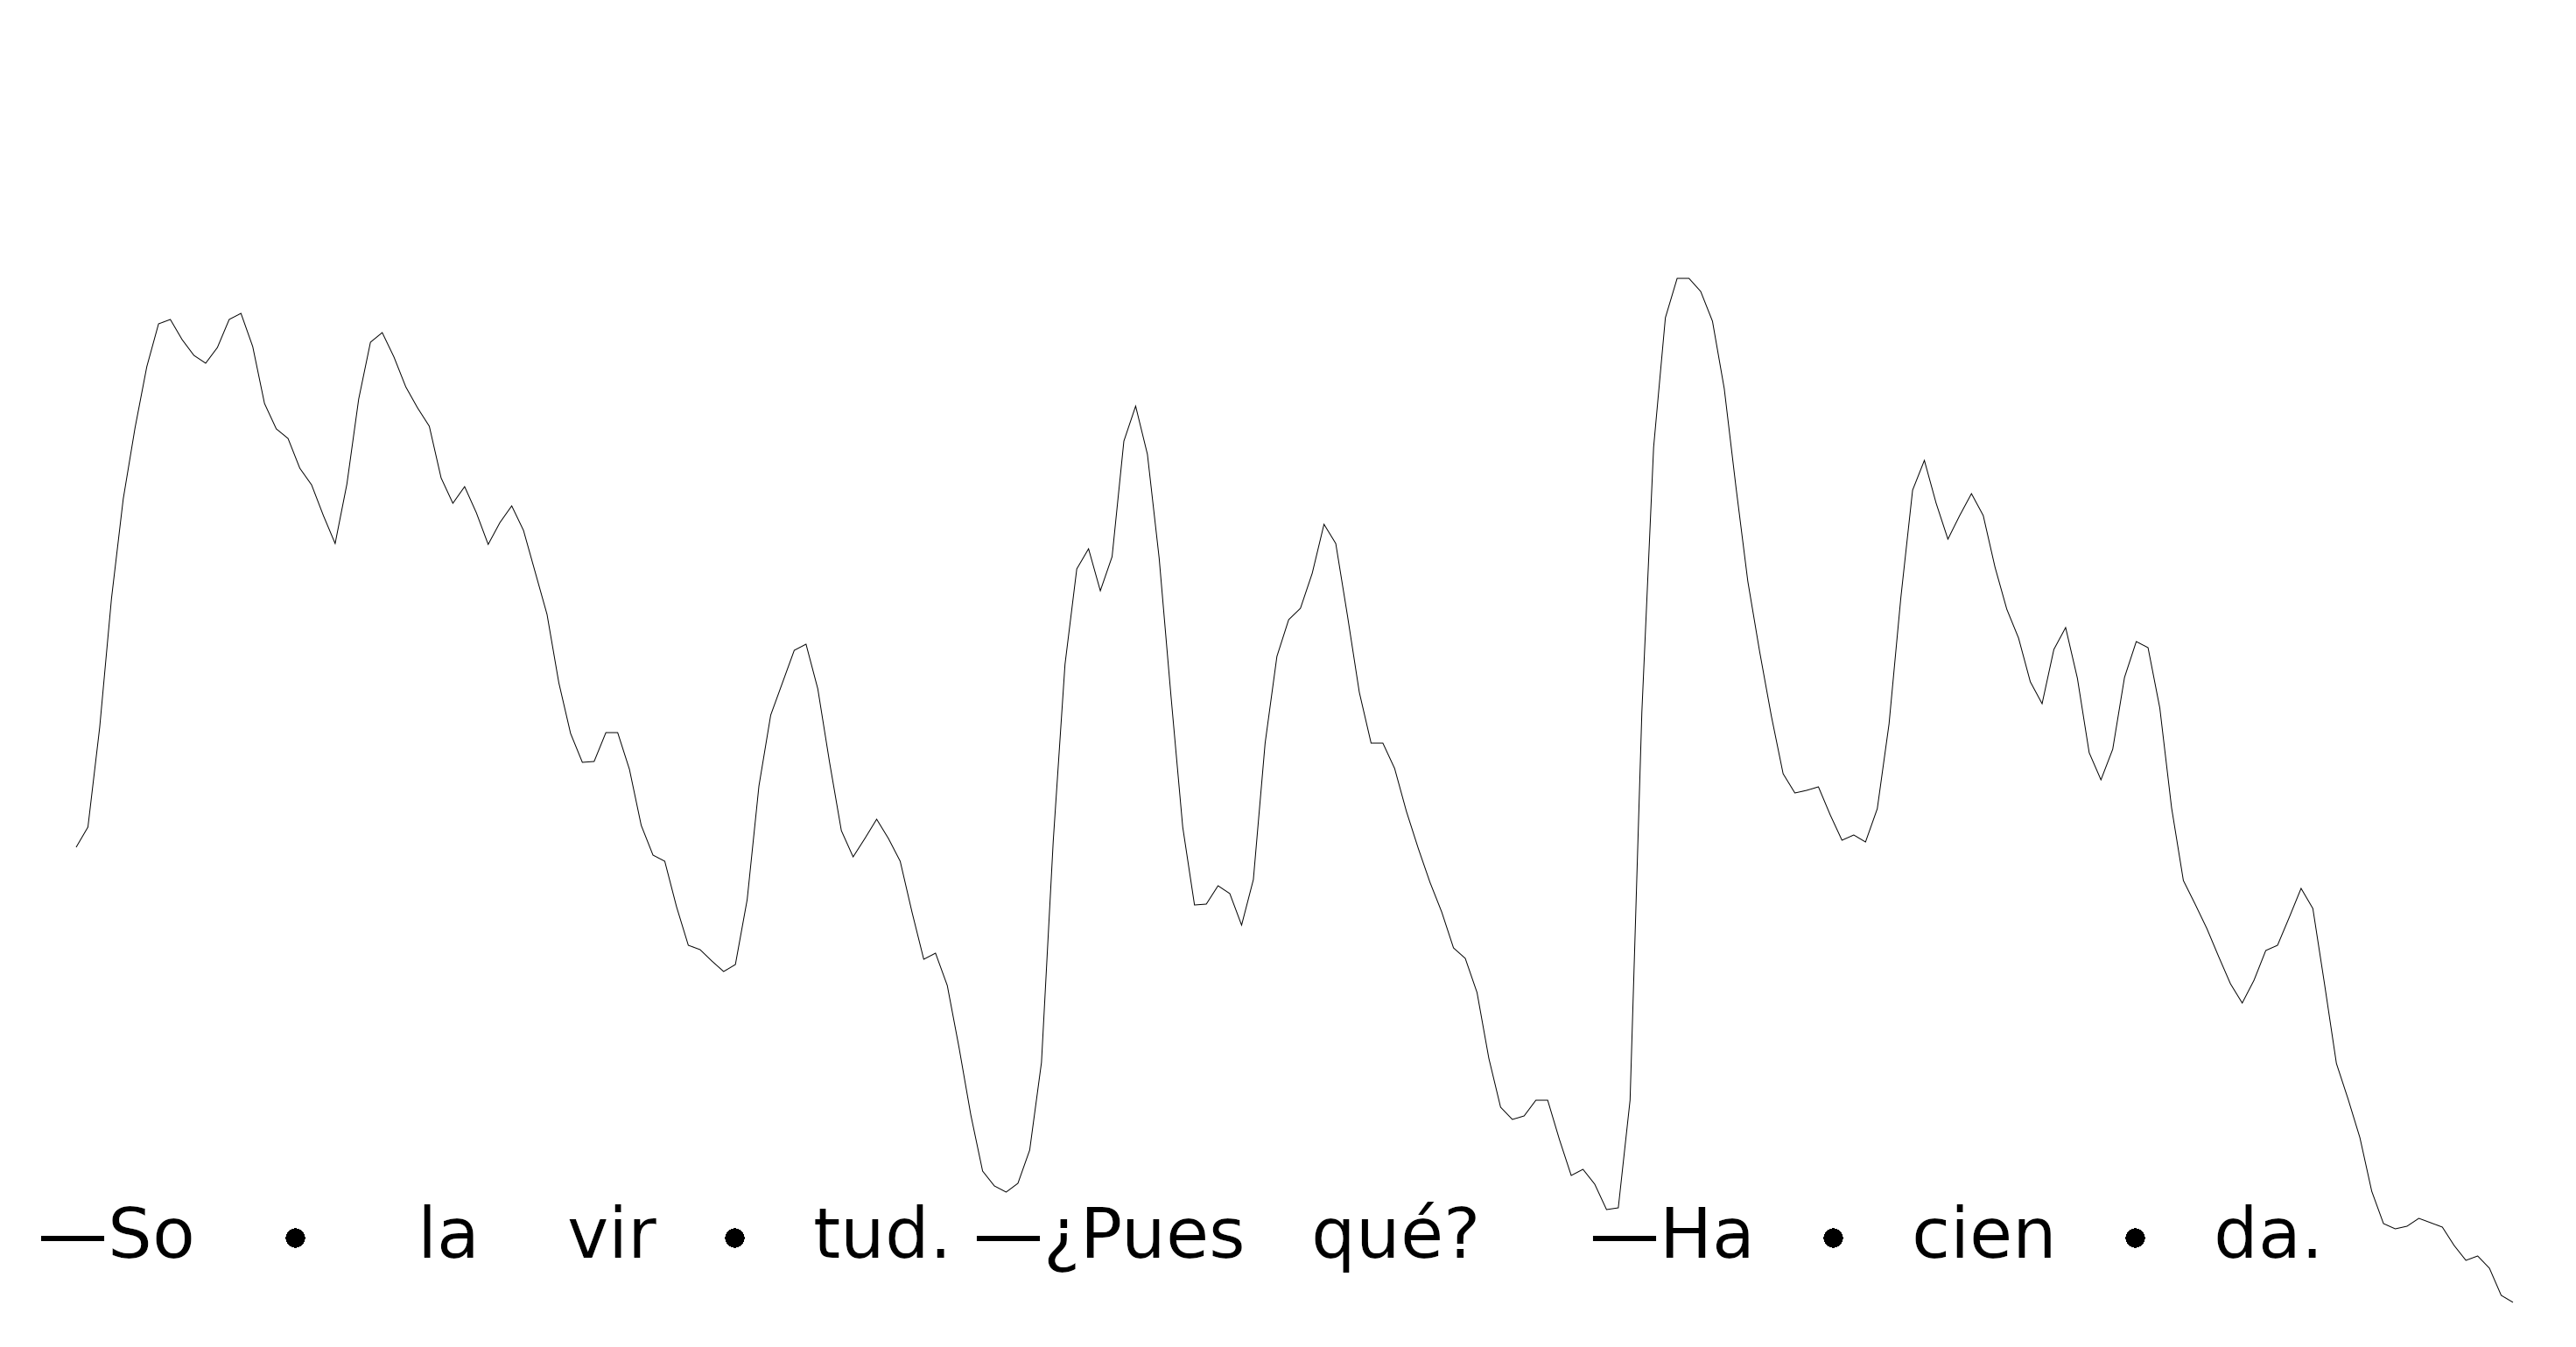
\includegraphics[height = 8cm]{images/solavirtud.png}    
	\caption{Verso 42 en una representación \parencite{vega1982} de \textit{La discreta enamorada}.}
	\label{fig:solavirtud}
\end{figure}

\subsection{Separación de vocales}
Se denomina \textit{diéresis}\index{diéresis} a la ruptura de  una unión natural entre vocales, de forma que el diptongo da lugar a dos sílabas independientes. En lo concerniente a nuestro trabajo, hay que tener en consideración que, a pesar de que estas vienen señaladas explícitamente en las ediciones más minuciosas (por ejemplo, \textlangle{}rüin\textrangle{} /ruˈin/ frente a \textlangle{}ruin\textrangle{} /ˈrwin/), no tiene por qué ser así en todos los casos y, de hecho, no suele serlo. Sin embargo, hay palabras cuyos diptongos se rompen de manera más frecuente en los versos áureos, como \textit{juez}, \textit{suave}, \textit{cruel}, \textit{fiel}, \textit{ruin} y sus derivados, por lo que, si se presenta la necesidad de producir una sílaba adicional para cuadrar el verso, este tipo de palabras se prestan sobremanera a la diéresis. Incluso vates tan poco dados a extravagancias como Quevedo recurren al hiato aprovechándolas, si bien con mucho más comedimiento que sus contemporáneos culteranos \parencite[55-64]{llamas2020}.

Otro fenómeno divisorio es el \textit{hiato}\index{hiato} o la ruptura de una sinalefa. Quilis~\parencite*[50-52]{quilis2013} atribuye el fenómeno a diversas causas, como la acentuación de una de las dos vocales implicadas, causa de sinalefa violenta. En la poesía del Siglo de Oro hay que contemplar asimismo la posible aspiración de la hache inicial en la segunda palabra que, como dijimos, también podría impedir la sinalefa.


\section{Rima}
El medio más evidente de alcanzar eufonía es la rima. Este recurso lírico consiste en la repetición de sonidos desde la última vocal acentuada o cumbre tonal\index{cumbre tonal} del verso. Puede ser de diferentes clases dependiendo de los tipos de sonido que se repitan \parencite[103-115]{dominguez2014a}. No es la única vía para crear un efecto melódico, sino que es frecuente encontrar también otras figuras de repetición tales como aliteración, simetría o anáfora \parencite[126-129]{dominguez2014a}. Podemos definir la rima, pues, como «la total o parcial semejanza acústica, entre dos o más versos, de los fonemas situados a partir de la última vocal acentuada» \parencite[37]{quilis2013}.

De esta manera, hablaremos de rima oxítona\index{rima!oxítona} o \textit{masculina}\index{rima!masculina|see {rima oxítona}} si el verso acaba en palabra aguda\index{palabra!aguda}, paroxítona\index{rima!paroxítona} o \textit{femenina}\index{rima!femenina|see {rima!paroxítona}} si acaba en palabra llana\index{palabra!llana} y proparoxítona\index{rima!proparoxítona} o dactílica\index{rima!dactílica|see {rima proparoxítona}} si acaba en palabra esdrújula\index{palabra!esdrújula}.

Caramuel~\parencite*[57]{caramuel2007} distingue entre rimas \textit{asonantes}\index{rima!asonante}, también llamadas parciales\index{rima!parcial|see {rima asonante}}, cuyas vocales coinciden, pero no así sus sonidos consonánticos (\ref{ex:asonante}), y rimas \textit{consonantes}\index{rima!consonante}, también llamadas rimas totales\index{rima!total|see {rima consonante}}, cuyas vocales y consonantes coinciden desde el último acento (\ref{ex:consonante}). 

\begin{exe}
	\ex\label{ex:asonante}
	\begin{tabular}{l|ll|}
		\cline{2-3}
		Yo, acudiendo a mis es-&t/\textit{ú}-& di/\textit{o}/s\\
		en ellos y en todo &m/\textit{í}-& r/\textit{o}\\
		que Segismundo se- &r/\textit{í}-& \textit{a}\\
		el hombre más atre-&v/\textit{í}-& d/\textit{o},\\\cline{2-3}
	\end{tabular}\\\strut\hfill(Calderón, \textit{La vida es sueño}, vv. 708-711\nocite{calderon_lavidaessuenno})
	\ex\label{ex:consonante}
	\begin{tabular}{l|l|}
		\cline{2-2}
		Hipogrifo vio-&l/\textit{énto},\\
		que corriste parejas con el&vi/\textit{énto}\\\cline{2-2}
	\end{tabular}\\\strut\hfill(vv. 1-2)	
\end{exe}

No todos los sonidos son parte de la rima. En el caso de la rima proparoxítona\index{rima!proparoxítona}, como ya indicamos, la constituyen los elementos de la sílaba tónica y la última sílaba (\ref{ex:proparox}), de manera que \textit{fábula} rima con \textit{águila}. En las rimas asonantes, solo los núcleos vocálicos son relevantes para la rima, de forma que \textit{inercia} rima con \textit{lenta} \parencite[89]{herrero1996}. Aquí es donde se hacen más vez patentes los beneficios de la decisión inicial de partir de una transcripción fonológica silabeada en lugar de la representación ortográfica (\ref{ex:as}). Por una parte, en tanto que tenemos el verso ya separado en sus sílabas, trabajaremos directamente con estas, corrigiendo según los fenómenos intervocálicos si es menester. Por otra parte, al distinguir entre los alófonos vocálicos silábicos y no silábicos, la resolución de la rima asonante es trivial, pues basta con tener en cuenta exclusivamente los fonemas vocálicos silábicos del \textit{axis}\index{axis rítmico} —que discutiremos abajo— de cada verso.

\begin{exe}
	\ex\label{ex:proparox}
	\begin{tabular}{l|l|l|l|}\cline{2-2}\cline{4-4}
	Al Uni-&gé-&ni-&to,\\
	al Padre &m/\textit{á}-&xi-&m/\textit{o}\\
	y al Santo Es-&pí-&ri-&tu,\\
	de ambos Pa-&r/\textit{á}-&cli-&t/\textit{o},\\
	pidamos &hú-&mi-&les,\\
	que en estos &\textit{á}/s-&pe-&r/\textit{o}-/s\\
	valles de &lá-&gri-&mas\\
	desiertos y &\textit{á}-&ri-&d/\textit{o}/s,\\
	su Amor a-&yú-&de-&nos,\\
	su Gracia &s/\textit{á}/l-&ve-&n/\textit{o}/s.\\
	\cline{2-2}\cline{4-4}
\end{tabular}\\
	\strut\hfill(Calderón, \citetitle[855-863]{calderon_annosantoroma})
\ex\label{ex:as}
	\begin{tabular}{l|ll|}\cline{2-3}
Que estas señoras da-&rán,&\\
de irlas sirviendo li-&c/\textit{é}/n-&ci/\textit{a}.\\
Y más cuando fuera& cul-&pa,\\
que los crïados que& d/\textit{é}-&j/\textit{a}/n\\
a sus dueños en vi-&si-&ta,\\
por ellos, Félix, no& vu/\textit{é}l-&v\textit{a}/n.\\
\cline{2-3}
\end{tabular}\\
	\strut\hfill(Calderón, \textit{¿Cuál es mayor perfección...?}, vv. 938-943\nocite{calderon_mayorperfeccion})
\end{exe}

Los versos que acaban con palabras homógrafas suponen un caso particular. Diremos que son \textit{equisonantes}\index{rima!equisonante} si estas difieren léxicamente o en su función gramatical, es decir, si se trata de una diáfora. Lo vemos en el ejemplo \ref{ex:equisonante}, donde \textit{pasa} toma el valor de `entrar' en el segundo de los versos, mientras que vale `acontecer' en el tercero. Si las palabras, además de ser homógrafas, también comparten significado y función, hablamos de rimas \textit{unisonantes}\index{rima!unisonante} (\ref{ex:unisonante}), que resulta inaceptable para la prescriptiva.
\begin{exe}
		\ex\label{ex:equisonante}
		[...]\\
		pero tu hermano viene. Aquí escondida\\
		le he de escuchar. Pues ya a tu cuarto \textit{pasa}.\\
		Y así saber espero lo que \textit{pasa}.\\
		\strut\hfill(Moreto, \textit{No puede ser el guardar una mujer}, vv. [1411-1413\nocite{moreto_nopuedeser})
	\ex\label{ex:unisonante}Colgad ese saco ahí\\
	para que diga, ay de \textit{mí}:\\
	«En tal puesto me colgó\\
	Paulo, que no mereció\\
	la gloria que encierro en \textit{mí}».\\
	\strut\hfill(Tirso de Molina, \citetitle[1885-1889]{tirso_desconfiado})                                         \end{exe}
En cualquier caso, estas restricciones solo afectan a la rima, por lo que, por ejemplo, el primer y segundo verso del ejemplo \ref{ex:norima} no estarían sujetos a estas restricciones y, si bien podría achacársele a Rojas Zorrilla un uso repetitivo del léxico en este caso, esto no tendría repercusión en su observancia de las reglas de la métrica.
\begin{exe}	
\ex\label{ex:norima}En tu atención. El amor,\\
¿quién le colige en lo a\textit{tento}?\\
La atención supone amor,\\
disgusto el diverti\textit{miento};\\
bien quiere aquel que escuchando\\
se transforma en los con\textit{cetos};\\
\strut\hfill(Rojas Zorrilla, \citetitle[31-36]{rojas_obligados})
\end{exe}

Sea como fuere, en el corpus que manejamos, el recurso a la equisonancia se utiliza de manera muy esporádica. La unisonancia es prácticamente inexistente, puesto que esta suele ser fruto de la falta de habilidad del poeta y, si las ediciones digitales de literatos áureos consagrados son escasas, más aún lo son las de los diletantes. La adscripción a uno u otro caso de homofonía de las ocurrencias que hemos encontrado suele ser susceptible de discusión. En cualquier caso, la máquina contaría con los medios para identificar estas rimas, ya que la determinación del ritmo\index{ritmo} obliga a identificar las funciones morfosintácticas de las palabras del verso. Por lo tanto, requeriría apenas verificar que ambos homógrafos de la rima tienen etiquetas diferentes.

Además de la rima externa, aparece aunque no resulta frecuente —Lope se vale de este recurso en, por ejemplo, \textit{El amigo hasta la muerte} y \textit{El mayordomo de la duquesa de Amalfi}— una rima interna italianizante, a imitación del \textit{endecasillabo incatenato}\index{verso!endecasílabo}. Esta rima interna la conforman las del axis rítmico y otro interno que pasa por la sexta sílaba, en el siguiente verso \parencite{sanchez2014}. 

\section{Agrupaciones de versos}
El verso por sí mismo no constituye un elemento lírico. Para que este sea digno de su nombre, debe aparecer en combinación con otros versos \parencite[95]{quilis2013}, de manera que formen una estructura superior que produzca el contexto sonoro de la poesía. Desde el punto de vista semántico, el verso es autosuficiente, pero no así desde el rítmico y sonoro, ya que ha de mostrar un patrón. Como es obvio, para que este pueda existir, se requiere, al menos, una serie de dos elementos. A esta agrupación estructurada de versos la denominamos estrofa\index{estrofa}. A su vez, cabe agrupar varias estrofas en un poema\index{poema!estrófico} estrófico, pero también pueden unirse versos directamente en poemas no estróficos\index{poema!no estrófico}.

\subsection{La estrofa}
De acuerdo con Quilis~\parencite*[95-99]{quilis2013}, la estrofa ha de cumplir cuatro requisitos para ser tal en propiedad: debe tener un \textit{axis rítmico}\index{axis rítmico}\footnote{Emplearemos este cultismo —que Quilis adopta de Balbín~Lucas~\parencite*{balbin1968} —, pues \textit{eje} \index{eje} podría llevar  a confusión, ya que también equivale a la sexta sílaba del endecasílabo\index{verso!endecasílabo} si esta va acentuada \parencite[][\textit{s.v.} \textit{eje}]{dominguez1985}.}, consistir de un número determinado de rimas, poseer una estructura sintáctica determinada y estar dispuesta según un modelo versal estructurado.

El axis rítmico, según como lo define Balbín~\parencite*[38-60]{balbin1968}, está constituido por la inflexión distensiva de cada uno de los grupos melódicos de los que se compone la estrofa en torno a la que se concentran y organizan los factores rítmicos.  Dicho de otra manera, el axis rítmico de la estrofa se establece a partir de la última sílaba acentuada de sus versos (\ref{ex:axis}). Esta es la que carga con el acento versal que, a su vez, altera la cantidad del verso. Aquí se produce asimismo la inflexión del tono; en torno a este punto se distribuyen las pausas para lograr la eufonía y se define el tipo de encabalgamiento.  El centro del eje provee el elemento más importante de la rima. En consecuencia, resulta crucial para nuestro modelo identificar esta parte del verso porque varios de los análisis que han de hacerse se sustentan en su correcta caracterización. Esto significa, además del silabeo, localizar la sílaba que carga con el acento léxico de la última palabra del verso.

\begin{exe}
	\ex\label{ex:axis}
		\begin{tabular}{l|l|l}
			\cline{2-2}
			¿cuál de vosotras, cuál desde su a-&\textit{si/é/n} & -to\\
			es la que influye en mí desdichas&	\textit{t/á}	& -les\\
			¿Cuál de vosotros, astros desi-&	\textit{gu/á}	& -les\\
		a su cargo tomó mi sufri-&				\textit{mi/é/n} & -to\\\cline{2-2}
		\end{tabular}\\
	\strut\hfill(Calderón, \citetitle[653-656]{calderon_suennoshay})
\end{exe}

El número de rimas resulta asimismo fundamental, pues la función de estas no se limita a la ejercida sobre el propio verso, sino que se combinan unas con otras de forma que, de esta unión, resulta una estrofa, cuya configuración es producto del número de rimas y de su distribución. Como veremos un poco más adelante, clasificamos las estrofas en primer lugar por el número de versos que las constituyen y, además, distinguimos entre estrofas con el mismo número de versos por la disposición de las distintas rimas de estos.

Por otra parte, la estrofa encuentra una correspondencia en la estructura sintáctica completa, de manera que la pausa estrófica coincide con el final de la unidad sintáctica. Aunque así se ha hecho tradicionalmente, algunos poetas con querencia por los modelos grecolatinos contravienen la prescriptiva de la métrica castellana para disociar una unidad sintáctica en dos estrofas \parencite[97]{quilis2013}. De la importancia de esta costumbre para reproducir el metro clásico da cuenta el elogio de Menéndez~Pelayo a Francisco Medrano, al que el erudito se refiere como \blockquote{de todos los imitadores de Horacio el más latino, el más sobrio, el más rápido, el que mejor ha remedado la marcha de los períodos rítmicos de Horacio, \textit{el que más se le parece en la manera de encabalgar las estrofas}, y el que más le anda a los alcances en el arte de economizar las palabras. \parencite[p. 14; énfasis añadido]{menendezpelayo1951}}.

En lo que respecta al sistema de estructurar las rimas, cada estrofa debe componerse de un número determinado de versos de tipos concretos dispuestos según un patrón dado. De esta manera, encontramos \textit{estrofas isométricas}\index{estrofa!isométrica}, en las que todos sus versos tienen la misma cantidad, como en el cuarteto del ejemplo \ref{ex:isometrica}, y \textit{estrofas heterométricas}\index{estrofa!heterométrica}, en las que se mezclan versos con distinto número de sílabas (\ref{ex:heterométrica}).

\begin{exe}
	\ex\label{ex:isometrica}Cuando la fama en lenguas dilatada\\	
	vuestra rara hermosura encarecía,\\
	por fe os amaba yo, por fe os tenía,\\ 		
	Leonor, dentro del alma idolatrada.\\
	\strut\hfill(Calderón, \citetitle[746-749]{calderon_secretoagravio})
	\ex\label{ex:heterométrica}Ilustre es, si no rico,\\
	el condado Anspurg en Alemania;\\
	a su quietud me aplico,\\
	pues los jardines de la gran Campania\\
	no igualan a este monte\\
	que el Ártico nos muestra en su horizonte.\\	
	\strut\hfill(Mira de Amescua, \citetitle[89-94]{mira_casaaustria})
\end{exe}
Para representar la estructura de las estrofas, emplearemos, además de la notación tradicional categórica de letras mayúsculas y minúsculas, la de subíndices si la caracterización de la estrofa requiere una descripción cuantitativa de sus versos. De esta manera, representaremos la estrofa del ejemplo \ref{ex:heterométrica} como \textit{aBaBcC} o $a_{7} b_{11} a_{7} b_{11} c_{7} c_{11}$, según las características que convenga observar en cada momento. La segunda forma resulta muy conveniente en una obra dramática, en la que, al contrario de lo que suele ocurrir en los poemas\index{poema}, se alternan diferentes metros, sobre todo de arte menor. De esta manera, resulta más sencillo explorar los versos en su contexto para conocer el uso de una determinada rima y condicionarlo al número de sílabas o viceversa.

Según la disposición de la rima en la estrofa, se distingue entre rima \textit{continua}\index{rima!continua}, con una estructura $aaaa$ (\ref{ex:continua}); \textit{rima gemela}\index{rima!gemela}, según el patrón $aa:bb$ (\ref{ex:gemela}); \textit{rima encadenada}\index{rima!encadenada}, con el patrón $abab$ (\ref{ex:encadenada}) y rima abrazada\index{rima!abrazada}, $abba$ (\ref{ex:abrazada}).

\begin{exe}
	\ex\label{ex:continua}Ay de opinión tan ciega,\\
	que los principios a la Fe le niega,\\
	donde a mover la Caridad no llega,\\
	que huye a Misericordia que le ruega!\\
	\strut\hfill(Calderón, \citetitle[779-982]{calderon_nuevohospicio})
	\ex\label{ex:gemela}Sí, mas de ambiguas razones\\
	en sus ojos mis pasiones\vspace{.333\baselineskip}\\
	han visto lo que me estima.\\
	Vana esperanza te anima\vspace{.333\baselineskip}\\
	cuando penetra mi amor\\
	el que me tiene interior.\vspace{.333\baselineskip}\\
	Cuando tu soberbia abajes\\
	y amor se obligue a mis gajes,\vspace{.333\baselineskip}\\
	tu engaño conocerás.\\
	Yo sé que me envidiarás.\\
	\strut\hfill(Tirso de Molina, \textit{Santo y sastre}, vv. 908-917)\nocite{tirso_santoysastre})
	\ex\label{ex:encadenada} Con el cuidado que el Amor, Diana,\\
	pone en un pecho, que aquel fin desea,\\
	que la mayor dificultad allana,\\
	Él mismo quiere que te adore y vea.\\
	\strut\hfill(Lope de Vega, \citetitle[689-692]{vega_perrohortelano}
	\ex\label{ex:abrazada}Tienes, Laurencia, razón;\\
	que en dejando de querer,\\
	más ingratos suelen ser\\
	que al villano el gorrión.\\ 
	\strut\hfill(\citetitle[249-242]{vega_fuenteovejuna})
\end{exe}


\subsection{Tipología estrófica}
Como indicamos al comienzo de este capítulo, el metro dramático no se diferencia del lírico. Por lo tanto, si hemos de encontrar patrones en las agrupaciones de versos, debemos recurrir a la poética tradicional. Añadiremos que el teatro no solo toma prestada la métrica de la poesía, sino que, además, lo hace extensivamente, aprovechando todos los recursos que aquella pone a su disposición. Así, Fernández Guillermo \parencite*[213-242]{fernandez2021} encuentra en apenas veinte comedias de Lope de Vega —un único autor— las siguientes formas: redondillas, romances con y sin estribillo con hexasílabos\index{verso!hexasílabo} y octosílabos\index{verso!octosílabo}, quintillas, pareados, tercetos sueltos y encadenados, endecasílabos\index{verso!endecasílabo} y otros versos sueltos, octavas, octavas reales, sonetos, canciones, décimas, sextinas, letrillas, coplas, coplillas, seguidillas, seguidillescas, glosas de tipos diversos, silvas, romancillos de ocho y siete sílabas, liras, sextetos-lira, cuartetas asonantadas, canciones petrarquistas, ensaladas, coplas de pie quebrado, villancicos y zéjel, así como partes cantadas con otras medidas y estrofas. A cuenta de esto, resulta necesario caracterizar las agrupaciones versales que encontraremos porque habremos de identificarlas en la segunda parte de este trabajo.

Nos aproximaremos a la clasificación estrófica típica del Siglo de Oro considerando formas recogidas por \citeauthor{morley1968}~\parencite*{morley1968} en su seminal trabajo sobre la datación de la obra lopesca. Optamos por este y no por la obra similar calderoniana de Hilborn~\parencite*{hilborn1938} por encontrarse esta última más simplificada \parencite[3-4]{antonucci2023}. Nos centraremos en las formas españolas \parencite[38-39]{morley1968} e italianas \citedate*[39-41]{morley1968}, como también los metros que constan en las tablas de \citeauthor{fernandez2021}~\parencite*[213-242]{fernandez2021}. Partiremos del número de versos que componen cada estrofa, tomando las descripciones de los tratados de métrica \parencites[102-153]{herrero1996}[100-119]{quilis2013}, e iremos ilustrando sus particularidades con ejemplos del corpus teatral. Esta clasificación será la que tomemos como modelo inicial para reconocer patrones en la segunda parte.

La estrofa más elemental es el \textit{pareado}\index{pareado}, ya que está compuesta de tan solo dos versos de igual o distinto metro y es autosuficiente. Al ser solo dos versos independientes del contexto, solo admiten un patrón de rima en la forma $AA$ (\ref{ex:pareado}). Si, además, los versos son octosílabos\index{verso!octosílabo} con rima consonante $a_{8}a_{8}$, la estrofa se denomina \textit{aleluya}\index{aleluya}. El pareado no ha de ser necesariamente isométrico, sino que también se da entre versos de distinta medida. Un ejemplo paradigmático lo ofrece la combinación de heptasílabos\index{verso!heptasílabo} y endecasílabos\index{verso!endecasílabo} de los pares de versos que componen la \textit{silva de consonantes}\index{silva!de consonante} del monólogo con el que Rosaura da comienzo a \textit{La vida es sueño} (\ref{ex:silvaconsonante}).

\begin{exe}
	\ex\label{ex:pareado}Éste dice: «Señor, yo soy Estacio,\\
		que estoy en los jardines de palacio,\vspace{.333\baselineskip}\\
		y enseñado a plantar hierbas y flores,\\
		planté seis hijos, a los dos mayores\vspace{.333\baselineskip}\\	
		suplico que les deis...».\\
		\strut\hspace{10em}Basta, ya entiendo,\\
		con más cuidado ya premiar pretendo.\\
	\strut\hfill(Lope de Vega, \citetitle[2467-2472]{vega2019})
	\ex \label{ex:silvaconsonante}Hipogrifo violento,\\
	que corriste parejas con el viento,\\
	¿dónde, rayo sin llama,\\
	pájaro sin matiz, pez sin escama,\\
	y bruto sin instinto\\
	natural, al confuso laberinto\\
	de esas desnudas peñas\\
	te desbocas, te arrastras y despeñas?\\
	\strut\hfill(Calderón, \citetitle[1-8]{calderon_lavidaessuenno})
\end{exe}

De cualquier manera, al haber una única rima posible, el nexo entre estrofas del mismo tipo ha de ser débil, en tanto que la siguiente o bien tiene la misma rima, en cuyo caso no hay un cambio, o una diferente, por lo que el salto será abrupto. No es factible una transición entre pareados que además sea suave. Para que esto sea posible, debemos contemplar la estrofa respecto a otras, lo que es el caso del \textit{perqué}\index{perqué} o \textit{aquelindo}\index{aquelindo|see {perqué}}, que alterna rimas que encadena con la siguiente estrofa según la estructura $ab/bc/cd/de...$

\begin{exe}
	\ex\label{ex:perque}\begin{multicols}{2}Escucha, la que veniste\\
	de la jerezana tierra\vspace{.333\baselineskip}\\	
	a hacer a Sevilla guerra\\
	en cueros, como valiente;\vspace{.333\baselineskip}\\	
	la que llama su pariente\\
	al gran Miramamolín;\vspace{.333\baselineskip}\\		
	la que se precia de ruïn,\\
	como otras de generosas;\vspace{.333\baselineskip}\\	
	la que tiene cuatro cosas,\\
	y aun cuatro mil, que son malas;\vspace{.333\baselineskip}\\	
	la que pasea sin alas\\
	los aires en noche escura;\vspace{.333\baselineskip}\\	
	la que tiene a gran ventura\\
	ser amiga de un lacayo;\vspace{.333\baselineskip}\\
	la que tiene un papagayo\\
	que siempre la llama puta;\vspace{.333\baselineskip}\\
	la que en vieja y en astuta\\
	da quinao a Celestina;\vspace{.333\baselineskip}\\
	la que, como golondrina,\\
	muda tierras y sazones;\vspace{.333\baselineskip}\\
	la que a pares, y aun a nones,\\
	ha ganado lo que tiene;\vspace{.333\baselineskip}\\
	la que no se desaviene\\
	por poco que se le dé;\vspace{.333\baselineskip}\\
	la que su palabra y fe\\
	que diese, jamás guardó;\vspace{.333\baselineskip}\\
	la que en darse a sí excedió\\
	a las godeñas más francas;\vspace{.333\baselineskip}\\
	la que echa por cinco blancas\\
	las habas y el cedacillo.\end{multicols}\strut\hfill(Cervantes, \citetitle[556-596]{cervantes1997})
\end{exe}

Del mismo modo, las transiciones entre estrofas se multiplican en el momento en que introducimos un nuevo verso. Las estrofas de tres versos se denominan \textit{tercetos}\index{terceto} en su versión de arte mayor $ABA$ (\ref{ex:terceto}) y tercerillas en las de arte menor\index{tercerilla} $aba$ (\ref{ex:tercerilla}). De esta manera, se dan estrofas $AAA$, que diferirían de los pareados en la cantidad de versos, aunque no en la cualidad de la rima, pero también $ABA$ o $ABB$, que introducirían una alternancia en la rima. Esto, a su vez, expande las posibilidades de combinar estrofas porque ahora podemos encadenarlas en la forma $ABA BCB CDC ...$, de modo que la nueva rima sirve de solución de continuidad para la transición de un verso, pero, al contrario que en la estrofa de dos sílabas, la estrofa puede conservar una rima característica distinta de la siguiente. En la poesía medieval se cultivaba una variante del terceto conocida como \textit{trístico monorrimo}\index{trístico monorrimo}, que tiene la misma rima en sus tres versos según el modelo $AAA$ (\ref{ex:tristico}).
  
 \begin{exe}
 	\ex\label{ex:terceto}Si yo pensara, Conde, que te diera\\
 		tanta tristeza el casamiento mío,\\
 		antes de imaginarlo me muriera.\\
 		\strut\hfill(Lope de Vega, \citetitle[114-116]{vega2019})
 	\ex\label{ex:tercerilla}Si aborrecidas adoran,\\
 	si adoradas aborrecen,\\                                              
 	¡lo que son mujeres!\\	
 	\strut\hfill(Rojas Zorrilla, \textit{Lo que son mujeres}, vv. 2849-2851\nocite{rojas_loquesonmujeres})
 	\ex\label{ex:tristico}Pues los músicos digan a coros:\\
 	No están todos\\
 	en la casa de los locos.\\	
 	\strut\hfill(vv. 2701-2703)
 	\end{exe}
 	
 	
Las estrofas de cuatro versos ofrecen más variedad. Si son consonantes de arte mayor, se denominan \textit{cuartetos}\index{cuarteto}, y tienen rima cruzada $ABBA$ o encadenada $ABAB$ (\ref{ex:cuarteto}), en cuyo caso reciben el nombre de \textit{serventesio}\index{serventesio}. En cuanto a las de arte menor, tenemos la \textit{cuarteta}\index{cuarteta} según el esquema $abab$ (\ref{ex:cuarteta}). La combinación de arte menor se conoce como \textit{redondilla}\footnote{No confundir con la \textit{redondilla} según la terminología de Díaz~Rengifo~\parencite*[193-207]{diazrengifo2012}, quien emplea el término para referirse a estrofas de octosílabos\index{verso!octosílabo} de cinco versos y sus variaciones de entre cuatro y ocho.}\index{redondilla} si la rima es abrazada en la forma $abba$ (\ref{ex:redondilla}). Una variante de esta estrofa es aquella que solo rima en sus versos pares según el modelo $-a-a$. Se da también la modalidad \textit{asonantada}\index{cuarteta!asonantada} o \textit{tirana}\index{cuarteta!tirana|see {cuarteta asonantada}} (\ref{ex:asonantada}). La redondilla en secuencia con el romance es la estrofa más común en el teatro de Lope \parencite[169]{fernandez2007}, cuya obra representa un porcentaje notable de la producción dramática del Siglo de Oro que ha llegado hasta nosotros. 

\begin{exe}
	\ex\label{ex:cuarteto}Amor de ser amado satisfecho\\
	cuando agraviado imaginó vengarse,\\
	Templado el fuego y el furor desecho,\\
	Adonde pudo arderse pudo helarse.\\
	\strut\hfill(Lope de Vega, \citetitle[403]{vega_dorotea})
	\ex\label{ex:cuarteta}Razón, fortuna, amor, celos\\
	son pasiones que se mudan:\\
	la razón falta a su tiempo\\
	y se cansa la fortuna;\\
	\strut\hfill(Calderón, \citetitle[2068-2071]{calderon_bandaflor})
	\ex\label{ex:redondilla}Yo os juro que, si os agrado,\\
	que de vos lo voy también,\\
	y que, procediendo bien,\\
	os doy amor por cuidado.\\
	\strut\hfill(Lope de Vega, \citetitle[65-68]{vega_villano})
	\ex\label{ex:asonantada}Inventó el amor un juego\\
	donde en gustosos descuidos,\\
	pagando en prendas sus yerros,\\
	se vino a quedar desnudo.\\
	\strut\hfill(Moreto, \textit{El hijo pródigo}, vv. 1309-1312\nocite{moreto_hijoprodigo})
\end{exe}

Las estrofas de cuatro versos se prestan bien a diversas combinaciones heterométricas. Así, la \textit{seguidilla}\index{seguidilla} combina versos impares heptasílabos\index{verso!heptasílabo} y pares pentasílabos en su variedad habitual (\ref{ex:seguidilla})\footnote{No confundir con la llamada \textit{seguidilla gitana}\index{seguidilla!gitana}, compuesta de versos hexasílabos\index{verso!hexasílabo} a excepción del tercero que es decasílabo o endecasílabo\index{verso!endecasílabo}, que sería una variante de la endecha \parencite[185-186]{hanssen1957}.}. Navarro Tomás\parencite*[292-293]{navarrotomas1991} recoge variaciones con hexasílabos en lugar de pentasílabos, así como de tres versos, que se reparten según las disposiciones $5-7-5$ y $7-5-7$, y \citeauthor{morley1968}~\parencite*{morley1968} con siete versos $XaYa:bZb$. Asimismo, Sor Juana Inés, entre otras modalidades, usó una conocida como \textit{seguidilla real}\index{seguidilla!real}, según el patrón $x{10}a_6x_{10}a_6$. También heterométrica es la \textit{estrofa sáfica}\index{estrofa!sáfica} (\ref{ex:estrofasafica}), que se compone de tres endecasílabos sáficos  (\texttt{---+x+xxx+-}) y un pentasílabo adónico (\texttt{+xx+x}) o, en su adaptación a la rítmica castellana, un hexasílabo según el patrón \texttt{+x+x+-} \parencite[119]{luque2010}. En la poética castellana, gozaba de gran tradición el \textit{tetrástrofo monorrimo}\index{tetrástrofo monorrimo|see {cuaderna vía}}, más conocido por \textit{cuaderna vía}\index{cuaderna vía}, que se compone de cuatro versos alejandrinos\index{alejandrino}, a su vez formados por dos hemistiquios\index{hemistiquio} heptasílabos cada uno, y una sola rima consonante, pero su presencia es escasa en el Siglo de Oro \parencite[277]{navarrotomas1991}. Entre las formas heterométricas destacan las que constituyen la composición conocida como \textit{endecha real}\index{endecha!real}  (\ref{ex:endechareal}). Si la \textit{endecha}\index{endecha} es un romancillo de versos de menos de ocho sílabas de tema triste \parencite[\textit{s.v.} \textit{endecha}]{dominguez1985}, la real presenta la particularidad de que sus tres primeros versos son heptasílabos y el cuarto endecasílabo.

\begin{exe}
	\ex\label{ex:seguidilla}Alegría, zagales,\\                                                                  
	que a casa vuelve\\
	hoy el hijo perdido.\\
	Todos se alegren.\\
	\strut\hfill(Moreto, \textit{El hijo pródigo}, vv. 2843-2856\nocite{moreto_hijoprodigo})
	\ex\label{ex:estrofasafica}\metrics{u | _ u u | _ u || u _ u u _ u ||}{{A-} | mor po-{de-} | ro-so || en cie-lo \bow{y e}n tie-rra, ||}\\	
\metrics{u | _ u u | _ u || u _ u u _ u ||}{{dul-} | cí-si-ma | gue-rra || de nues-tros sen-ti-dos, ||}\\
\metrics{u | _ u u | _ u || u _ u u _ u ||}{¡oh, | cuán-tos {per-} | di-dos || con vi-d\bow{a i}n-quï-e-ta ||}\\
\metrics{u | _ u u | _ u ||}{{t\bow{u i}m-} | pe-rio {su-} | je-ta! ||}\\
	\strut\hfill(Lope de Vega, \citetitle[158]{vega_dorotea})
	\ex\label{ex:endechareal}No con más diligencia\\
	la diosa de las mieses\\
	buscó a su hija amada\\
	hasta los escondrijos del infierno,\\
	\strut\hfill(Cervantes, \citetitle[515-518]{cervantes_entretenida})
\end{exe}

Hay que hacer notar una característica del ejemplo \ref{ex:estrofasafica} que será conveniente considerar para diseñar el sistema de escansión. Si atendemos a la prosodia, la estrofa está compuesta de tres versos de doce  sílabas y uno de seis. Sin embargo, dijimos que este tipo de estrofa se compone de endecasílabos\index{verso!endecasílabo} y un pentasílabo. Vemos en la correspondencia con los pies del modelo latino del pentasílabo y los primeros hemistiquios\index{hemistiquio} de los endecasílabos que tenemos una sílaba suelta antes del dáctilo y el troqueo. En efecto, está sílaba está en anacrusa, por lo que no se considera en el cómputo silábico ni en el patrón acentual —de cantidad en el modelo latino—. De esta manera,  los acentos de los endecasílabos recaen en la primera y cuarta sílaba tras la anacrúsica y en la primera y tercera en el pentasílabo. Dada la escasa frecuencia con que aparecen metros inusuales, cabe plantearse considerar este fenómeno ante versos de metro inesperado con sílabas átonas a comienzo del verso. Por otra parte, el último endecasílabo presenta otra particularidad, ya que requiere contemplar la interjección como inacentuada.

Entre las estrofas isométricas de cinco versos, el \textit{quinteto}\index{quinteto}, de arte mayor, no es habitual en la poesía aurisecular, al contrario que su equivalente de arte menor, la \textit{quintilla}\index{quintilla} (\ref{ex:quintilla}). Ambas formas presentan restricciones, pues han de tener rima consonante, no contienen más de dos versos seguidos con la misma rima, los dos últimos versos no riman entre sí y no hay versos sueltos, de manera que solo se dan las combinaciones $ABABA$, $ABAAB$, $ABBAB$, $AABAB$ y $AABBA$. Entre las estrofas heterométricas cabe destacar la \textit{lira}\index{lira}, que combina dos endecasílabos\index{verso!endecasílabo} y tres heptasílabos\index{verso!heptasílabo} según la estructura rimante $aBabB$. Aunque apenas encuentra uso dramático tras Rey de Artieda y Juan de la Cueva \parencite[257]{navarrotomas1991}, da pie a otros metros más extendidos como el sexteto-lira.

 \begin{exe}
	\ex\label{ex:quintilla}Y así, en lirio transformado,\\
	siendo el morado color\\
	jeroglífico del prado,\\
	se vio entre el lirio y la flor\\
	el amor enamorado.\\	
	\strut\hfill(Calderón, \textit{Hado y divisa...}, vv. 1604-1608\nocite{calderon_hadoydivisa})
	\ex\label{ex:lira}¿Es, ingrata Sigura,\\
	el casamiento próspero que aguardo?\\
	Callar será cordura,\\
	pues de ira y desdén ardo,\\
	y de envidia me hielo y acobardo.\\
	\strut\hfill(Rey de Artieda, \citetitle[533-537]{reydeartieda_amantes})
\end{exe}

Las estrofas isométricas de seis versos más destacadas son la \textit{sextilla}\index{sextilla} (\ref{ex:sextilla}), con restricciones semejantes a las de la quintilla en cuanto a la disposición de las rimas, así como su equivalente de arte mayor, el \textit{sexteto}\index{sexteto}. La \textit{sextina real}\index{sextina!real} o \textit{sexta rima}\index{sexta rima|see {sextina real}} es una configuración italianizante de versos endecasílabos\index{verso!endecasílabo} según el patrón $ABABCC$, «como una octava real a la que hubiesen recortado los dos primeros versos» \parencite[276]{baehr1997}. Presenta a veces algunas variaciones, como el empleo de versos oxítonos\index{rima!oxítona} en los versos tercero y sexto; no obstante, gozó de escasa estima entre los dramaturgos áureos \parencite[256]{navarrotomas1991}.

\begin{table}[!ht]
	\centering\small
	\begin{tabular}{rlcc}
		\toprule
		Versos&Estrofa&Rima&Distribución\\
		\midrule
		\multirow{4}{*}2&Pareado&indiferente& $a_{x}a_{x}$\\
		&Aleluya&indiferente&$a_{8}a_{8}$\\
		&Perqué&indiferente&$a_{8}b_{8}/b_{8}c_{8}/...$\\
		&Silva de consonantes.&consonante&$a_{7}a_{11}$\\
		\midrule
		\multirow{4}{*}3&Tercerilla&consonante&$aba$\\
		&Terceto&consonante&$a_{11}b_{11}a_{11}$\\
		&Trísticos&indiferente&$a_{x}a_{x}a_{x}$\\\midrule
		\multirow{9}{*}4&Cuarteta&consonante&$abab$\\
		&Redondilla&consonante&$abba$\\   
		&Serventesio&consonante&$ABAB$\\
		&Cuarteto&consonante&$ABBA$\\
		&Copla&asonante&$xaxa$\\
		&Seguidilla&indiferente&$x_{7}a_{5}x_{7}a_{5}$\\
		&Cuaderna vía&consonante&$x_{14}x_{14}x_{14}x_{14}{}^{*}$\\
		&Estrofa sáfica&indiferente&$x_{11}x_{11}x_{11}x_{5}$\\\midrule
		\multirow{3}{*}5&Quintilla&indiferente&$abbab{}^{\dag}$\\
		&Quinteto&consonante&$ABBAB{}^{\dag}$\\
		&Lira&indiferente&$a_{7}b_{11}a_{7}b_{7}b_{11}$\\\midrule
		\multirow{6}{*}6&Sextilla&consonante&$abaaba{}^{\dag}$\\
		&Sexteto&consonante&$ABAABA{}^{\dag}$\\
		&Sexteto correlativo&consonante&$a_{7}b_{7}c_{11}/a_{7}b_{7}c_{11}$\\
		&sexteto-lira&consonante&$a_{7}b_{11}a_{7}b_{11}c_{7}c_{11}$\\
                &Sexta rima&consonante&$a_{11}b_{11}a_{11}b_{11}c_{11}c_{11} / a_{11}c_{11}c_{11}^{\prime}b_{11}b_{11}c_{11}^{\prime}$\\
                &Estrofa manriqueña&consonante&$a_{8}b_{8}c_{4}a_{8}b_{8}c_{4}$\\\midrule
		\multirow{2}{*}7&Séptima&indiferente&$abbab$\\
                &Seguidilla compuesta&indiferente&$x_{7}a_{5}x_{7}a_{5}\:b_{7}a_{5}x_{7}b_{5}$\\\midrule
		\multirow{5}{*}8&Octavilla&consonante&$a_{8}b_{8}b_{8}c_{8}^{\prime}\:d_{8}e_{8}e_{8}c_{8}^{\prime}$\\
		&Octava real&consonante&$a_{11}b_{11}a_{11}b_{11}a_{11}b_{11}c_{11}c_{11}$\\
                &Copla castellana&consonante&$a_{8}b_{8}b_{8}a_{8}\:c_{8}d_{8}d_{8}c_{8}$\\
		&Copla de arte mayor&consonante&$a_{12}b_{12}b_{12}a_{12}\:a_{12}c_{12}c_{12}a_{12}$\\
		&Octava italiana&consonante&$ABBE^{\prime}\: CDDE^{\prime}$\\\midrule
		\multirow{3}{*}{10}&Décima&consonante&$abba\:ac\:cddc$\\
		&Copla real&consonante&$abbab\:cdcdc$\\
                &Ovillejo&consonante&$a_{8}a_{4}b_{8}b_{4}c_{8}c_{4}\:c_{8}d_{8}d_{8}c_{8}$\\
		\bottomrule
		\multicolumn{4}{l}{\footnotesize\textsuperscript{*} También de dieciséis sílabas.}\\
		\multicolumn{4}{l}{\footnotesize${}^{\dag}$ Las rimas alternas de acuerdo a las restricciones descritas.}\\
	\end{tabular}
	\caption{Estrofas.}
	\label{tab:estrofas}
\end{table}


Encontramos asimismo estrofas\index{estrofa!heterométrica} heterométricas, como el sexteto-lira\index{sexteto-lira}, compuesto de heptasílabos\index{verso!heptasílabo} y endecasílabos\index{verso!endecasílabo} en versos alternos, tal como en $aBaBcC$ o $abCabC$ (\ref{ex:sextetolira}). Existen también combinaciones heterométricas de arte menor, como la sextilla\index{sextilla! de pie quebrado} \textit{de pie quebrado}\footnote{También aparece como \textit{copla de pie quebrado}\index{copla!de pie quebrado|see {sextilla de pie quebrado}} (\ref{ex:coplapiequebrado}). Sin embargo, dado que la copla tiene un tamaño variable, optaremos por denominar este metro como sextilla en lugar de utilizar el \textit{hiperónimo} copla.}. Un caso particular de esta estrofa con gran tradición en las letras castellanas es la llamada \textit{estrofa manriqueña}\index{estrofa!manriqueña}, por haberla usado Jorge Manrique en el siglo \textsc{xv} para componer las \textit{Coplas a la muerte de su padre}. En esta estrofa, los tetrasílabos se disponen en el tercer y sexto verso, tal que resulta $a_{8}b_{8}c_{4}a_{8}b_{8}c_{4}$. También de seis versos son las \textit{estrofas aliradas}\index{estrofa!alirada}, que alternan endecasílabos y heptasílabos según el esquema $aBaBcC$ (\ref{ex:estrofalirada}), pero que admiten además otras combinaciones.

\begin{exe}
	\ex\label{ex:sextilla}Si lo que la Infanta yerra\\
	peregrino huésped, curas,\\
	haciendo al infierno guerra,\\
	dirán todas las criaturas:\\
	«¡Gloria a Dios en las alturas,\\
	y paz al hombre en la tierra!».\\
	\strut\hfill(Calderón, \citetitle[1328-1334]{calderon_venenotriaca})
	\ex\label{ex:sextetolira}Aneguen mis enojos\\
	estos campos con llanto de mis ojos.\\
		Y este monte, que ha sido\\
		áspero monumento,\\
		aumente el sentimiento,\\
		aun sin tener sentido,\\
		y, enternecido, el suelo\\
		muestre en su llanto eterno desconsuelo,\\
	\strut\hfill(Calderón, \textit{Judas Macabeo}, vv. 492-497\nocite{calderon_judasmacabeo})
	\ex\label{ex:coplapiequebrado} ¡Qué ventura\\
	que solo el tiempo os destroce,\\
	cuando el sol solo os conoce;\\
	y en esta selva segura,\\
	lo que vuestra vida dura,\\
	libres siempre, nadie os goce!\\	
	\strut\hfill(Calderón, \citetitle[299-304]{calderon_secretoagravio})
	\ex\label{ex:estrofalirada}Un sabio que escribía\\
	en su cama, una vez incorporado,\\
		la mano que movía,\\
		por ser entonces el invierno helado,\\
		de suerte se le helaba\\
		que apenas letra ni razón formaba.\\
	\strut\hfill(Lope de Vega, \textit{Poder vencido y amor premiado}, vv. 3033-3038\nocite{vega_podervencido})
\end{exe}

Las estrofas\index{estrofa} de siete versos no resultan tan productivas en las letras castellanas como las otras que hemos visto. Mencionaremos la \textit{seguidilla compuesta}\index{seguidilla!compuesta} entre las estrofas de este número de sílabas, que se compone de una seguidilla simple y un bordón o estribillo de tres versos adicionales, distribuidos según la forma $x_{7}a_{5}x_{7}a_{5}/b_{5}x_{7}b_{5}$. No obstante, la estrofa varía en sus versos según el bordón. Asimismo, encontramos una extensión a siete versos de la estrofa alirada repitiendo el metro en los dos últimos (\ref{ex:entretenida}).
\begin{exe}
	\ex\label{ex:entretenida}Amor, que lo imposible facilitas\\	
	con poderosa fuerza blandamente,\\
	allanando las cumbres:\\
	¿por qué las nubes de mi sol no quitas?\\
	¿Por qué no muestras por algún Oriente\\	
	las dos hermosas cumbres\\
	que dan rayos al sol, luz a tus ojos,\\
	por quien te rinde el mundo sus despojos?\\
	\strut\hfill(Cervantes, \citetitle[577-584]{cervantes_entretenida})
\end{exe}

Las estrofas de ocho versos gozan de mayor estima en la literatura española. La agrupación isométrica de arte mayor más típica es la \textit{octava}, pero existen diferentes variantes de esta. Así, se conocen estrofas como la \textit{copla de arte mayor}\index{copla!de arte mayor} —también llamada de Juan de Mena, por haberla cultivado este poeta con gran acierto—, que adopta el patrón $a_{12}b_{12}b_{12}a_{12}:a_{12}c_{12}c_{12}a_{12}$. Sin embargo, es muy difícil de encontrar en el teatro del Siglo de Oro. La configuración típica de la copla de arte menor es $abba:acca$ \parencite[266]{navarrotomas1991}. La \textit{octava real}\index{octava real} surge como una modificación de la octava real siciliana, en la que se altera la última rima para obtener un pareado en acorde a $ABABABCC$ (\ref{ex:octavareal}), y se emplea en el teatro para parlamentos graves \parencites[252]{diazrengifo2012}[255]{navarrotomas1991}.

\begin{table}[!ht]
	\centering\small
	\begin{tabular}{llll}
		\toprule
		Enfático&puro&&1-6-10\\
		Enfático&pleno&&1-6-8-10\\
		Heroico&puro&&2-6-10\\
		Heroico&pleno&&2-4-6-8-10\\
		Heroico&corto&&2-4-6-10\\
		Heroico&largo&&2-6-8-10\\
		Heroico&difuso&&2-4-10\\
		Melódico&puro&&3-6-10\\
		Melódico&pleno&&1-3-6-8-10\\
		Melódico&largo&&3-6-8-10\\
		Melódico&corto&&1-3-6-10\\
		Sáfico&puro&&4-8-10\\
		Sáfico&puro&pleno&1-4-8-10\\
		Sáfico&pleno&&1-4-6-8-10\\
		Sáfico&corto&&4-6-10\\
		Sáfico&corto&pleno&1-4-6-10\\
		Sáfico&largo&&4-6-8-10\\
		Sáfico&largo&pleno&2-4-8-10\\
		Sáfico&difuso&&4-10\\
		Sáfico&difuso&pleno&1-4-10\\
		Sáfico&inverso&&1-6-7-10\\
		Vacío&puro&&6-10\\
		Vacío&largo&&6-8-10\\
		Dactílico&puro&&4-7-10\\
		Dactílico&pleno&&1-4-7-10\\
		Dactílico&corto&&2-4-7-10\\
		Galaico&antiguo&&5-10\\
		Italiano&puro&&7-10\\
		\bottomrule
	\end{tabular}
	\caption{Clasificación del endecasílabo.}
	\label{tab:endecasilabos}
\end{table}



En cuanto a las estrofas\index{estrofa!de arte menor} de arte menor, desde el Renacimiento se encuentran \textit{octavillas}\index{octavilla}, pero estas no son más que la unión de dos redondillas en las que una de sus rimas es coincidente. Para el periodo que nos ocupa, entendemos la estrofa como una composición de otras menores, ya que no adquiere entidad propia hasta entrado el siglo \textsc{xviii}, cuando se introduce la \textit{octavilla italiana}\index{cuarteta italiana}, que aporta el rasgo distintivo del último verso agudo de cada semiestrofa. La \textit{copla castellana}\index{copla!castellana} no difiere en esto, aunque sí en la rima de la segunda semiestrofa, de manera que presenta un patrón de según el modelo $abba:cddc$  (\ref{ex:coplacastellana}). Esta forma tuvo cierto predicamento hasta la época de Juan de la Cueva, pero las siguientes generaciones optaron por la redondilla emancipada \parencite[267]{navarrotomas1991}. Pueden ser también de \textit{de pie quebrado} si alternan versos de ocho y cuatro sílabas.

\begin{exe}
	\ex\label{ex:octavareal}«Señor, mirad por vuestra casa atento;\\
	que el Conde y la Duquesa en vuestra ausencia...»\\
	No me ha sido traidor el pensamiento,\\
	habrán regido mal, tendré paciencia.\\
	«ofenden con infame atrevimiento\\
	vuestra cama y honor», ¿Qué resistencia\\
	haran a tal desdicha mis enojos?\\
	«Si sois discretom os lo diran los ojos».\\
	\strut\hfill(Lope de Vega, \citetitle[2484-2491]{vega2019})
	\end{exe}

Las últimas estrofas\index{estrofa} que repasaremos en este capítulo son las compuestas de diez versos. No iremos más allá, puesto que estamos de lleno en el terreno en el que las agrupaciones se consideran estructuras complejas a partir de la combinación de estrofas simples. Sirva para ilutrarlo la copla castellana del ejemplo \ref{ex:coplacastellana}, que podría dividirse en dos estrofas simples, redondillas en este caso. De esta manera, una vez hayamos establecido en la parte práctica el modo de agrupar las estrofas simples, podremos extrapolar el método a cualquier otra forma compleja para clasificarla según patrones estróficos, análogamente a lo hecho con los versos.

\begin{exe}
	\ex\label{ex:coplacastellana}A Dios pongo por testigo,\\
	si a tal quisiera venir,\\
	mas puédeseme decir:\\
	«mensajero sois, amigo».\\
	Que bien saneado estó\\
	que dirán de mi llegada:\\
	«aunque traéis la embajada,\\
	no merecéis culpa, no»\footnote{Nótese que se emplea este metro tradicional para tratar un tema clásico del romancero. No resulta probable que esto sea producto de la mera casualidad, sino que, más bien, sugiere una percepción de la copla castellana como una estrofa arcaizante, lo que bien podría explicar el desuso en el que cayó con la llegada de la Edad Moderna.}.\\	
	\strut\hfill(Juan de la Cueva, \textit{La muerte del rey don Sancho...}, vv. 172-178\nocite{mena_muertereysancho})
\end{exe}

 Así, entre las estrofas de diez versos citaremos la \textit{copla real}\index{copla!real}, que podría analizarse en realidad como la unión de dos quintillas; la \textit{décima}\index{décima} o \textit{espinela}\index{espinela|see {décima}} —ya que se atribuye su invención al ingenio de  Vicente Espinel—, que, a su vez, está compuesta de dos redondillas unidas por dos versos de enlace en los que se repite la primera rima de cada una de las redondillas (\ref{ex:decima}) y, por último, el \textit{ovillejo}\index{ovillejo} o \textit{séptima real}\index{séptima real|see {ovillejo}}, una forma compuesta de tres pareados\index{pareado} octosilábicos y tetrasilábicos y una redondilla\index{redondilla} octosilábica (\ref{ex:ovillejo}).
 
 Existen no obstante construcciones estróficas de verso variable, como la \textit{estancia}\index{estancia}, que combina entre nueve y veinte versos heptasílabos\index{verso!heptasílabo} y endecasílabos\index{verso!endecasílabo} con rima consonante. En su modalidad más regular, consta de una \textit{fronte}\index{fronte@\textit{fronte}|see {frente}} o \textit{frente}\index{frente} y una \textit{sirma}\index{sirma@\textit{sirma}|see {coda (metro)}} o \textit{coda}\index{coda (metro)}. La frente la componen dos \textit{piedi}\index{piede@\textit{piede}|see {pie (metro)}} o \textit{pies}\index{pie (metro)} de tres versos e igual esquema rítmico, denominado el primero \textit{vuelta} o \textit{tornata} y el segundo \textit{revuelta}. La coda comienza con un \textit{eslabón}  (también \textit{chiave}\index{chiave@\textit{chiave}|see {eslabón}}) heptasílabo que rima con el último verso de la fronte, al que siguen otros versos hasta concluir con una coda de pareados. 

\begin{exe}
	\ex\label{ex:decima}\begin{multicols}{2}
	Dorotea: litigantes\\
	sobre tu amor, Lelio y yo,\\
	la esperanza nos citó\\
	a tus estrados amantes.\vspace{.333\baselineskip}\\
	
	Amigos éramos antes;\\
	mas pleitos de tu beldad\vspace{.333\baselineskip}\\	
	mudan nuestra voluntad\\
	en competencia enemiga,\\
	que si es cuerdo, no hay quien diga\\
	que en pleitos hay amistad.\end{multicols}
	\strut\hfill(Tirso de Molina, \textit{Santo y sastre}, vv. 847-856\nocite{tirso_santoysastre})
	\ex\strut\label{ex:ovillejo}\begin{multicols}{2}
		Céfiro, ¿en quién dicha espera?\\
		En una fiera.\vspace{.333\baselineskip}\\
		¿Y quién a Ifis da desmayo?\\
		Un bello rayo.\vspace{.333\baselineskip}\\
		¿En quién Pigmaleón no medra?\\
		En una piedra.\vspace{.333\baselineskip}\\
		\vspace{.333\baselineskip}\\
		Ninguno llegue a ser yedra\\
		del laurel que ama, porque hoy\\
		lloren todos, que yo soy\\
		la fiera, el rayo y la piedra.\\
	\end{multicols}	
	\strut\hfill(Calderón, \citetitle[2060-2069]{calderon_fierarayopiedra})
\end{exe}


\subsection{Poemas estróficos}
Denominamos poemas\index{poema!estrófico} estróficos a aquellos que, como su propio nombre sugiere, están compuestos por estrofas. Esto es, los versos se agrupan en unidades intermedias dentro del poema. En la literatura española se han usado con más o menos profusión diferentes formas, pero los siguientes ocupan un lugar destacado \parencite[126-150]{quilis2013}.

La \textit{canción}\index{canción} es un tipo de poema\index{poema} que proporciona gran libertad compositiva al poeta, ya que, además de no exigirle fijar un número de estrofas concreto, estas también varían en su número de versos. En general, las estrofas\index{estrofa} oscilan entre seis y doce versos en la canción provenzal o nueve y veinte en la petrarquista, así como quince en el modelo de Boscán o trece el de Garcilaso. Tampoco hay una regla fija que dicte la naturaleza de la rima y su distribución. A pesar de todo, hay una estructura global fija, ya que la disposición de la primera estrofa se repite en las siguientes. Cada una de estas estrofas tiene dos partes, unos versos iniciales de frente, que se divide a su vez, por lo general, en dos pies, y una parte final o coda, compuesta por uno más versos o uno o más \textit{volte}\index{volta@\textit{volta}}\footnote{Tomaremos prestado el término de la nomenclatura italiana porque la forma \textit{verso} podría inducir a confusión con uso más común en la métrica.} a imagen de los pies de la frente. La canción concluye con una estrofa más corta, la \textit{tornata}\index{tornata@\textit{tornata}|see {envío}} o \textit{envío}\index{envío}. Puede darse asimismo un eslabón de unión entre frente y coda. Su presencia en el teatro es escasa, aunque no del todo desconocida. En el ejemplo \ref{ex:cancion}, frente y coda tienen dos partes de cuatro versos, el envío también de cuatro y sin verso de enlace.

\begin{exe}
	\ex\label{ex:cancion}\begin{multicols}{2}Llorente pidió a su prima\\
	Constanza le dé a beber,\\
	y ella quísolo hacer\\
	y echóle el cántaro encima.\vspace{.333\baselineskip}\\
	Sintiéndose fatigado\\
	de sed, de amor y calor,\\
	le demandó por favor\\
	agua, estando ya abrasado.\vspace{.333\baselineskip}\\
	No se esquiva aunque se estima,\\
	y en empezando a beber\\
	ella le dejó caer\\
	el cántaro todo encima.\vspace{.333\baselineskip}\\
	Rió, desque así lo vido,\\
	y él comenzó a sacudirse,\\
	y acometió para irse,\\
	colorado de corrido.\vspace{.333\baselineskip}\\
	Ella dijo: — ¿Esto os lastima?\\
	Torna si queréis beber,\\
	y dejaros he caer\\
	el cántaro y agua encima\vspace{.6\baselineskip}
\end{multicols}
\strut\hfill(Juan de la Cueva, \textit{Los siete
	infantes de Lara}, vv. 503-522 \nocite{cueva1924})\end{exe}


La \textit{glosa}\index{glosa} carece de una extensión fija. Se caracteriza por componerse de una poesía breve llamada \textit{texto}\index{texto} y la glosa propiamente dicha, que consiste en un comentario al anterior distribuido en tantas estrofas (décimas\index{décima} por lo general) como versos componen el texto. Deberemos, pues, verificar si hay repeticiones de versos y si la estructura métrica sugiere una poesía de este tipo. En el ejemplo \ref{ex:glosa}, tenemos el texto en la primera estrofa\index{estrofa} en cursiva, seguido de una quintilla que anuncia la glosa de décimas que sigue, cuyo último verso —correspondiente al texto, o sea, a la primera quintilla— hemos enfatizado también mediante letra cursiva.

\begin{exe}
	\ex\label{ex:glosa}\begin{multicols}{2}\textit{En fin, señora, me veo}\\
	\textit{sin mí, sin vos, y sin Dios.}\\
	\textit{Sin Dios, por lo que os deseo;}\\
	\textit{sin mí, porque estoy sin vos;}\\
	\textit{sin vos, porque no os poseo.}\vspace{.222\baselineskip}\\
	Y por si no lo entendéis,\\
	haré sobre estas razones\\
	un discurso, en que podréis\\
	conocer de mis pasiones\\
	la culpa que vos tenéis.\vspace{.222\baselineskip}\\
	Aunque dicen que el no ser\\
	es, señora, el mayor mal,\\
	tal por vos me vengo a ver,\\
	que para no verme tal,\\
	quisiera dejar de ser.\\
	En tantos males me empleo,\\
	después que mi ser perdí,\\
	que aunque no verme deseo,\\
	para ver si soy quien fui,\\
	\textit{en fin, señora, me veo.}\vspace{.222\baselineskip}\\
	A decir que soy quien soy,\\
	tal estoy, que no me atrevo,\\
	y por tales pasos voy,\\
	que aun no me acuerdo que debo\\
	a Dios la vida que os doy.\\
	Culpa tenemos los dos,\\
	del no ser que soy agora,\\
	pues olvidado por vos\\
	de mí mismo, estoy, señora,\\
	\textit{sin mí, sin vos y sin Dios.}\vspace{.222\baselineskip}\\
	Sin mí no es mucho, pues ya\\
	no hay vida sin vos, que pida\\
	al mismo que me la da;\\
	pero sin Dios, con ser vida,\\
	¿quién si no mi amor está?\\
	Si en desearos me empleo,\\
	y él manda no desear\\
	la hermosura que en vos veo,\\
	claro está que vengo a estar\\
	\textit{sin Dios, por lo que os deseo.}\vspace{.222\baselineskip}\\
	¡Oh, qué loco barbarismo\\
	es presumir conservar\\
	la vida en tan ciego abismo\\
	hombre que no puede estar\\
	ni en vos, ni en Dios, ni en sí mismo.\\
	¿Qué habemos de hacer los dos,\\
	pues a Dios por vos perdí,\\
	después que os tengo por dios,\\
	sin Dios, porque estáis en mí,\\
	\textit{sin mí, porque estoy sin vos?}\vspace{.222\baselineskip}\\
	Por haceros sólo bien,\\
	mil males vengo a sufrir;\\
	yo tengo amor, vos desdén,\\
	tanto, que puedo decir:\\
	¡mirad con quién y sin quién!\\
	Sin vos y sin mí peleo\\
	con tanta desconfianza.\\
	Sin mí porque en vos ya veo\\
	imposible mi esperanza;\\
	\textit{sin vos, porque no os poseo.}\end{multicols}	
	\strut\hfill(Lope de Vega, \citetitle[1916-1975]{vega2019})
\end{exe}

La \textit{sextina}\index{sextina} está formada por seis estrofas\index{estrofa!de arte mayor} de seis versos de arte mayor no rimados acabados en seis sustantivos\index{sustantivo} diferentes de dos sílabas pero en un orden distinto en cada estrofa, y una \textit{contera}\index{contera}, que es una estrofa de tres versos que contiene los seis sustantivos en la forma $ABCDEF$ $FAEBDC$ $CFDABE$ $ECBFAD$ $DEACFB$ $BDFECA$ $A\text{-}B$ $D\text{-}E$ $C\text{-}F$ (\ref{ex:sextina}). Sin embargo, los dramaturgos de la época se prodigaron poco en ella, aunque aún se encuentran en unas pocas obras de comienzos del siglo \textsc{xvii}.

\begin{exe}
	\ex\label{ex:sextina}Hermosas, claras, cristalinas fuentes,\\			
		jardines frescos, celebrados árboles,\\
		que aquí me vistes de Jarifa hermano,\\
		ya no soy el hermano de Jarifa;\\
		ya puedo ser su amante y ser su esposo:\\
		dad todos parabién a Abindarráez.\vspace{.333\baselineskip}\\			
		Ya no soy aquel triste Abindarráez\\
		que os daba tanto llanto, puras fuentes;\\
		ya no escribiré hermano, sino esposo,\\
		por las cortezas de los verdes árboles.\\
		Pero, si no me quiere mi Jarifa,\\				
		¡cuanto mejor me fuera ser su hermano!\vspace{.333\baselineskip}\\
		Mas aunque no me quiera, el ser su hermano\\
		ya quita la esperanza a Abindarráez\\
		de la gloria que el alma ve en Jarifa.\\
		Dirán que esto es verdad las sordas fuentes,\\			
		y sus hojas harán lenguas los árboles:\\
		tanto es el bien de poder ser su esposo.\vspace{.333\baselineskip}\\
		Si solo el ser posible ser su esposo\\
		estorbaba del todo el ser su hermano,\\
		jardines, hiedras, flores, plantas, árboles,\\
		aquí donde lloraba Abindarráez,\\
		hechos sus ojos caudalosas fuentes,\\
		aquí se llama esposo de Jarifa.\vspace{.333\baselineskip}\\
		¡Cielos! ¿Que gozar puedo de Jarifa?\\
		¿Que ya es posible que yo sea su esposo?\\
		Riendo lo murmuran estas fuentes,\\
		que me llamaron tristemente hermano.\\
		Decid que soy su esposo Abindarráez,\\
		que el viento os dará voz, amigos árboles.\vspace{.333\baselineskip}\\
		¡Que de veces al pie de aquestos árboles\\
		miré los bellos ojos de Jarifa,\\
		y ella me dijo: «¡Hermano Abindarráez!»\\
		Pues ya su esposo soy, no soy su hermano;\\
		o, a lo menos ya puedo ser su esposo:\\
		decidselo, si vuelve, claras fuentes.\vspace{.333\baselineskip}\\
		Fuentes, ya cesa el llanto; verdes árboles,\\
		ya parto a ser esposo de Jarifa,\\
		que ya no soy su hermano Abindarráez.\\
	\strut\hfill(Lope de Vega, \textit{El remedio en la desdicha}, vv. 309-437 \nocite{vega_remediodesdicha})
\end{exe}

El popular \textit{soneto}\index{soneto} (\ref{ex:soneto}) gozó del mayor reconocimiento entre los poemas\index{poema} de endecasílabos\index{verso!endecasílabo} en el Siglo de Oro \parencite[252]{navarrotomas1991}. Se caracteriza por sus catorce versos de once sílabas en su modalidad más extendida, divididos en dos cuartetos y dos tercetos, cuyo esquema clásico es $ABBA$ $ABBA$ $CDC$ $DCD$, aunque admite otras combinaciones. En los tercetos, siguen al modelo clásico en popularidad $CDE:CDE$, $CDE:DCE$, $CDC:EDE$, $CDE:DEC$, $CDC:CDC$ y $CDE:EDC$, sin que un poeta se incline necesariamente siempre por una u otra variante.

\begin{exe}
	\ex\label{ex:soneto}Apenas el hibierno helado y cano\\
	este monte con nieves encanece,\\
	cuando la primavera le florece\\
	y el que helado se vio se mira ufano.\vspace{.333\baselineskip}\\
	Pasa la primavera y el verano\\
	los rigores del sol sufre y padece;\\
	llega el fértil otoño y enriquece\\
	el monte de verdor, de fruta el llano.\vspace{.333\baselineskip}\\
	Todo vive sujeto a la mudanza:\\
	de un día y otro día los engaños\\
	cumplen un año, y este al otro alcanza.\vspace{.333\baselineskip}\\
	Con esperanza sufre desengaños\\
	un monte que, a faltarle la esperanza,\\
	ya se rindiera al peso de los años.\\	
	\strut\hfill(Calderón, \citetitle[1385-1398]{calderon_econarciso2})
\end{exe}

El \textit{villancico}\index{villancico} es una composición versos octosílabos\index{verso!octosílabo} u hexasílabos\index{verso!hexasílabo} que se divide en dos partes: un \textit{estribillo}\index{estribillo} de entre dos y cuatro versos $xa$ y un \textit{pie de estrofa}\index{pie de estrofa} de seis o siete versos $xxxxaa$, los últimos de los cuales riman con el estribillo (\ref{ex:villancico}).

\begin{exe}
	\ex\label{ex:villancico}Entra mayo y sale abril,\\
	¡cuán garridico le vi venir!\vspace{.333\baselineskip}\\
	Entra mayo coronado\\
	de rosas y de claveles,\\
	dando alfombras y doseles\\
	en que duerma amor, al prado.\\
	De trébol viene adornado,\\
	de retama y toronjil.\vspace{.333\baselineskip}\\
	Entra mayo y sale abril,\\
	¡cuán garridico le vi venir!\\
	\strut\hfill(Tirso de Molina, \textit{La peña de Francia}, vv. 2045-1006\nocite{tirso_penafrancia})
\end{exe}

El {zéjel}\index{zéjel} es una composición usualmente de versos octosílabos\index{verso!octosílabo} que está formada por un estribillo\index{estribillo} de uno o dos versos (a), una segunda estrofa llamada \textit{mudanza}\index{mudanza} de tres versos monorrimos (b) y un último verso o \textit{vuelta}\index{vuelta} (c) que rima con el estribillo, quedando en la distribución $aa:bbba$ (\ref{ex:zejel}).

\strut\begin{exe}\ex\label{ex:zejel}\begin{multicols}{2}¡Ay, Fortuna,\\
	cógeme esta aceituna!\vspace{.333\baselineskip}\\
	Aceituna lisonjera,\\
	verde y tierna por defuera,\\
	y por de dentro madera,\\
	fruta dura e importuna.\vspace{.333\baselineskip}\\
	¡Ay, Fortuna,\\
	cógeme esta aceituna!\vspace{.333\baselineskip}\\
	Fruta en madurar tan larga\\
	que sin aderezo amarga;\\
	y aunque se coja una carga,\\
	se ha de comer sola una.\vspace{.333\baselineskip}\\
	¡Ay, Fortuna,\\
	cógeme esta aceituna!\end{multicols}
	\strut\hfill(Lope de Vega, \citetitle[2043-2056]{vega_villano})
\end{exe}

\subsection{Poemas no estróficos}
Además de los poemas\index{poema!estrófico} estróficos, los versos se agrupan también por sí mismos en otras estructuras métricas de extensión variable sin necesidad de estar integrados en uniones intermedias como la estrofa\index{estrofa}. Existen varios tipos de poemas no estróficos de extensión variable que aparecen de manera recurrente en la literatura castellana \parencites[150-169]{quilis2013}[254]{navarrotomas1991}. El más relevante de todos ellos para este trabajo es, tal vez, el \textit{romance}\index{romance} (\ref{ex:romance}), tanto por su tradición como por la profusión con la que los poetas lo han usado, pero, sobre todo, por ser la agrupación variable más común del teatro áureo. Se trata de una serie ilimitada de octosílabos\index{verso!octosílabo} con rima asonante en los pares y suelta en los impares. En su vertiente culta, estos se agrupan en cuartetas y suele intercalarse un estribillo popular con heptasílabo\index{verso!heptasílabo} o endecasílabo\index{verso!endecasílabo}, un pareado de octosílabos con rima diferente al romance, o un dístico endecasílabo con la misma rima. No es extraño encontrar combinaciones de metros diferentes, como octosílabos y hexasílabos\index{verso!hexasílabo}.

\begin{exe}
	\ex\label{ex:romance}\begin{multicols}{2}Un gallardo caballero\\
	hermosamente vestido\\
	a nuestra quinta ha llegado.\\
	¡Ay, Lauro, yo soy perdido,\\
	sin duda, es aqueste el rey!\\
	¿Quién es?\\\strut\hspace{4em}Es un hombre erguido,\\
	tan resuelto y tan bizarro\\
	que solo de haberle visto\\
	vengo temblando de miedo.\\
	El rey es.\\
	\strut\hspace{4em}Él no ha pedido\\
	licencia, que ya se ha entrado.\\
	¿Qué hay, Elena?\\
	\strut\hspace{7em}Señor mío,\end{multicols}
	\strut\hfill(Enríquez Gómez, \textit{Engañar para reinar}, vv. 777-788\nocite{enriquez_enganarreinar})
\end{exe}
Aparte del habitual romance octosilábico, en la métrica castellana se da también una variedad menor de este, compuesta de versos de menos de ocho sílabas, que se denomina \textit{romancillo}\index{romancillo} (\ref{ex:romancillo}). También relacionado con el romance, así como con el villancico, encontramos el poema\index{poema} llamado \textit{letrilla}, que se compone de un número indeterminado de redondillas o quintillas dobles y un estribillo o dos alternados. Suele constar de versos octosílabos\index{verso!octosílabo} o hexasílabos\index{verso!hexasílabo} y aparece indistintamente con rimas asonantes y consonantes. 

\begin{exe}
	\ex\label{ex:romancillo}\begin{multicols}{2}¡Ay, riguroso estado,\\ausencia mi enemiga,\\
	que dividiendo el alma\\
	puedes dejar la vida!\\
	¡Cuán bien por tus efetos\\
	te llaman muerte viva,\\
	pues das vida al deseo\\
	y matas a la vista!\\
	¡Oh, cuán piadosa fueras,\\
	si al partir de Medina\\
	la vida me quitaras\\
	como el alma me quitas!\\
	En ti, Medina, vive\\
	aquella Inés divina,\\
	que es honra de la corte\\
	y gloria de la villa.\\
	Sus alabanzas cantan\\
	las aguas fugitivas,\\
	las aves, que la escuchan\\
	las flores, que la imitan.\\
	Es tan bella que tiene\\
	envidia de sí misma,\\
	pudiendo estar segura\\
	que el mismo sol la envidia;\\
	pues no la ve más bella,\\
	por su dorada cinta,\\
	ni cuando viene a España\\
	ni cuando va a las Indias.\\
	Yo merecí quererla.\\
	¡Dichosa mi osadía,\\
	que es merecer sus penas\\
	calificar mis dichas!\\
	Cuando pudiera verla,\\
	adorarla y servirla,\\
	la fuerza del secreto\\
	de tanto bien me priva.\\
	Cuando mi amor no fuera\\
	de fe tan pura y limpia,\\
	las perlas de sus ojos\\
	mi muerte solicitan.\\
	Llorando por mi ausencia\\
	Inés quedó aquel día,\\
	que sus lágrimas fueron\\
	de sus palabras firma.\\
	Bien sabe aquella noche\\
	que pudiera ser mía.\\
	Cobarde amor, ¿qué aguardas,\\
	cuando respetos miras?\\
	¡Ay, Dios, qué gran desdicha,\\
	partir el alma y dividir la vida!\end{multicols} 
	\strut\hfill(Lope de Vega, \citetitle[1610-1659]{vega_caballeroolmedo})
\end{exe}

Un poco menos frecuente que el romance, pero también de gran popularidad en el teatro del Siglo de Oro, es la \textit{silva}\index{silva} (\ref{ex:silva}). Esta combina normalmente versos heptasílabos\index{verso!heptasílabo} y endecasílabos\index{verso!endecasílabo} con rima total, aunque admite versos sueltos intercalados y construcciones con endecasílabos exclusivamente. Junto a la silva hallamos el \textit{madrigal}\index{madrigal}, que comparte con aquella la carencia de una cantidad fija de estrofas o versos por estrofa y también hace combinaciones variables de heptasílabos y endecasílabos. Lo que diferencia una y otra composición es que la segunda expresa un pensamiento amoroso de extensión breve. En términos computacionales, esto implica que hay que plantear una hipótesis en consonancia con el número de versos porque, para identificar el tema automáticamente, habría que emplear técnicas de \textit{topic modelling}\index{topic modelling@\textit{topic modelling}}, lo que incrementaría la complejidad del trabajo\footnote{No obstante, este es un campo que hemos empezado a explorar con vistas a futuras investigaciones.}. 

\begin{exe}
	\ex\label{ex:silva}Cuestión fue, no apurada hasta este día,\\
	¿cuál hace más, aquel que desafía\\
	a otro a un sitio aplazado,\\
	o el que al sitio salió desafiado?\\
	Y bien ahora pudiera\\
	la cuestión resolver el que me viera\\
	batallando conmigo,\\
	porque no hay tan cruel fiero enemigo,\\
	como es el pensamiento del que aguarda.\\
	Mucho don Félix tarda.\\
	Sin duda que ha escogido,\\
	de don Diego celoso y ofendido,\\
	verse con él primero.\\
	Mas yo no cumpliré si no le espero.\\
	¿Quién en el mundo, cielos,\\
	se vio, sin dama, sin amor, sin celos,\\
	en tal lance empeñado?\\
	¡Que el prestar a un amigo mi criado\\
	de suerte lo disponga,\\
	que mi opinión en tal empeño ponga!\\
	Digo que aquestos días\\
	toda mi vida es caballerías,\\
	pues no hallo en ella cosa\\
	que parecer no pueda fabulosa.\\
	Una dama tapada me ha dejado,\\
	sin decirme quién es, enamorado;\\
	un criado me ha puesto,\\
	porque así su ignorancia lo ha dispuesto,\\
	en trance de perderme; y un amigo,\\
	sin quererlo, me ha dado un enemigo.\\
	Mas ¿qué me admiro? Si hallo a cada paso\\
	que estos son los empeños de un acaso.\\	
	\strut\hfill(Calderón, \citetitle[2046-2076]{calderon_empenosacaso})
\end{exe}

Asimismo, encontramos \textit{poemas de versos sueltos}\index{poema!de versos sueltos}, que responden a diversas necesidades, como el afán de imitar los modelos latinos o adaptarse a partes cantadas. Todavía más complicada llega a ser la \textit{ensalada}\index{ensalada}, que no solo mezcla metros a discreción sino también métricas, ya que aúna varios idiomas \parencites[314]{diazrengifo2012}[\textit{s.v.} \textit{ensalada}]{dominguez1985}. En estos casos, habremos de dejar la clasificación a la mano humana porque, además de reconocer palabras, ritmos\index{ritmo} y rimas\index{rima}, obligaría a identificar lenguas y métricas distintas a la silábica castellana, lo que sobrepasa las posibilidades de esta investigación y requeriría un trabajo propio.  

 Usaremos en cualquier caso esta selección de agrupaciones como base clasificatoria de la parte empírica del trabajo, a la que podremos añadir otras más específicas a la vista de los versos sueltos que resultaren de procesar el corpus de pruebas.
\label{chap:5}
			\part{Aplicación empírica}
				\chapter{De la teoría a la práctica}\label{chap:B1}
\epigraphhead[50]{\epigraph{Es muy misteriosa, llena de figuras y cifras, oscura y no patente para todos. Tienen sus vocablos y maneras de hablar muy diferente significación de la que saben los vulgares trilingües. Por donde el que construyera la letra y tomare el sentido que resulta de la construcción gramatical caerá en muchos errores.}{Juan Huarte de San Juan, \textit{Examen de ingenios para las ciencias}}}
\section{Computador y papel}
Bien pertrechados de fundamentos teóricos sobre los que sostener el análisis de los textos, podemos por fin abordarlos empíricamente con garantías. En esta segunda parte formalizaremos lo visto hasta ahora para instruir al computador sobre el modo de aplicarlo a los textos y extraer de ellos la información requerida. ¿De qué manera lo haremos? Como adelantamos en la introducción, la idea es ir tomando lo expuesto en la parte que acabamos de concluir y formalizarlo en esta parte práctica empleando una notación algorítmica de \textit{pseudocódigo}\footnote{Llamamos \textit{pseudocódigo}\index{pseudocódigo} o lenguaje de descripción algorítmica a una representación informal compacta del paradigma de un algoritmo. Su función no es ser interpretado por una máquina, sino mostrar el principio operativo del algoritmo.}. En cierto modo, lo que ofrecen estas páginas no va a dejar de seguir siendo un desarrollo teórico, pues no usaremos código fuente \textit{real} de un lenguaje de programación específico que pueda ser copiado y ejecutado directamente en un computador, sino que encontraremos la idealización de formalizaciones generales. Estas idealizaciones se representan mediante una tecnología que ha probado su valía durante milenios: la escritura. Si bien intentaremos descomponer cada proceso en bloques relativamente sencillos para que puedan ser seguidos sin dificultad, un papel y un bolígrafo podrían ser de ayuda para orientarse en los pasos menos evidentes. 

Son tres las razones que nos animan a plantear la labor de esta manera y no comentando los listados de código del lenguaje de programación en el que hemos hecho las pruebas. En primer lugar, conviene proponer una idea de la forma más clara y concisa posible, por lo que haremos bien en abstraernos de las particularidades a las que están sujetos los lenguajes de programación. Estos obligan a emplear una sintaxis estricta y funciones muy específicas propias de cada uno de ellos, lo que exige descomponer las ideas abstractas en procesos menores concretos, más por satisfacer necesidades técnicas que conceptuales. Esto es, deberíamos atenernos a la literalidad de la computación de según unas reglas particulares y renunciar a los atajos contextuales que confieren al lenguaje natural su agilidad. Incluso cuando hay una traducción estructural biunívoca, existen diferencias en cómo expresar el desarrollo que requeriría aclaraciones. No solo serían así mucho más largos los listados —lo que sería un inconveniente menor—, sino también más farragosos y, por lo tanto, difíciles de seguir, lo que ya sí es una preocupación de primer orden.

En segundo lugar, cada lenguaje posee de un repertorio propio de expresiones internas con las que ejecutar operaciones sintéticas. Sin embargo, obligaría a hacerlo analíticamente allá donde no. Aunque todos los lenguajes suelen ser capaces de realizar operaciones elementales, la disponibilidad de recursos para abordar otras más complejas varía de un lenguaje a otro. Estas últimas —como, por ejemplo, aquellas relacionadas con el \ac{pln}— requieren \textit{bibliotecas}\footnote{Un \textit{biblioteca}\index{biblioteca} (\textit{library} en inglés, por lo que, con más frecuencia de la deseable, hay que leer traducido con el barbarismo \textit{librería}) es una colección externa de funciones que un programa importa para usarlas como propias.} externas en el mejor de los casos; en el peor, obligan a elaborar los procedimientos desde cero. Sea como fuere, aunque estas bibliotecas actúan como una caja negra cuyo mecanismo interno es ajeno al programa que las invoca, los datos de entrada, que hay que facilitarles, y los de salida, que devuelven, pueden variar significativamente en su formato, incluso cuando son conceptualmente equivalentes. Esta diferencia en el repertorio de los diferentes lenguajes hace que, como decimos, recurrir a uno en concreto ilustraría el uso particular en este, pero complicaría la traducción a otros. De ahí que el pseudocódigo sea una buena alternativa tanto por una cuestión didáctica como por su generalidad.

En tercer lugar, en relación con lo anterior, la explicación en un lenguaje de programación concreto ha de presuponer cierta familiaridad con algunos elementos sintácticos fundamentales que, de lo contrario, requerirían ser explicados. Dado que este no es el sitio apropiado para ello, una sistematización sin otras particularidades que las propias de una notación general facilitan la comprensión, si bien a cambio de llenar los huecos que deja la falta de un lenguaje de programación real con el sentido común del lector.

Sin embargo, no debemos olvidar que el objeto de este trabajo es práctico, queremos dar una solución a un problema real y, no solo eso,  la solución debe ser empírica. Por esa razón, no  dejaremos lo aquí expuesto en el mundo inteligible, sino que produciremos su realización sensible. Dicho de otro modo, no ha de preocuparse el lector, pues le ahorraremos el trabajo de traducir los algoritmos aquí presentados en programas informáticos: para poner a prueba lo discutido programamos una implementación completa en Python 3\index{Python}, la misma que, una vez depurada, se ha estado usando en el proyecto \textit{Sound and Meaning}, cuya última versión disponible a fecha de la entrega de este trabajo se encuentra en los apéndices o, en un formato más conveniente y en su última versión disponible, en los repositorios públicos que se han habilitado en Internet para ello.

Como ya habíamos adelantado, la ubicación de este capítulo antecediendo a la formalización de los aspectos teóricos no responde a la casualidad. Al contrario, se trata de una elección que —creemos— ayuda a comprender el resto del trabajo. En ese sentido, este capítulo es un puente entre los textos y programas reales y la idealización de estos que usaremos en los capítulos siguientes. Aquí se explica  la elección de bibliotecas externas y otras diseñadas \textit{ad hoc} en las que delegarlas, así como sus interrelaciones. Esto no es obvio y solo cobra sentido si se conoce de antemano la estructura de dependencia de los módulos en la implementación del modelo. Asimismo, tras el presente capítulo, asumiremos textos en condiciones ideales y no está de más conocer que llegar a ellos no es una cuestión trivial. Excúsese, pues, este interludio técnico.

\section{Modelo de pruebas}
Como hemos dicho, en esta segunda parte no encontraremos el prototipo final. En su lugar, trazaremos un plano en los siguientes capítulos para explicar qué ha de hacerse, aunque sin entrar más de lo estrictamente necesario en cómo ha de llevarse a cabo. Hallaremos, por ejemplo, \textit{listas}, pero no una forma concreta de añadirles nuevos elementos o recorrerlas, ya que esto entraría en las particularidades de cada lenguaje de programación: damos por hecho que el lector es capaz de componer mentalmente una lista y recorrerla de la manera que considere oportuno. Permanecemos, pues, en el ámbito de las ideas. Este capítulo contiene asimismo el conjunto de especificaciones técnicas del prototipo que pretendemos construir a partir de las instrucciones del «plano». El producto final, el resultado de aplicar todo esto —más bien su fotografía, como captura inerte del modelo real— es lo que encontramos en los apéndices.

\subsection{Lenguaje de programación}
Para realizar la implementación del modelo, podríamos haber empleado cualquiera de los muchos lenguajes de programación disponibles en el mercado, pues no faltan aquellos con capacidad para representar con sencillez las estructuras de datos y algoritmos que requerimos. No obstante, nos decidimos por la versión 3 de Python\index{Python} por varias razones que pasamos a detallar.

Nos hacemos una idea de las cualidades de este lenguaje de programación a partir de su definición como «\textit{general-purpose programming language that blends procedural, functional, and object-oriented paradigms}» \parencite[p. 6, énfasis en el original]{lutz2013}. Esto es, tenemos un lenguaje que permite abordar todo tipo de tareas y aproximarse a ellas según diferentes paradigmas. Concretamente, la orientación a objetos de Python contempla la encapsulación y reutilización sin complicaciones \parencite[xiii]{bird2009}. En la última década, Python se ha convertido en uno de los lenguajes de programación más importantes para tratamiento de datos, \textit{machine learning}\index{machine learning@\textit{machine learning}} y desarrollo de \textit{software} tanto en la academia como en la industria \parencite[2]{mckinney2018}.

Python es, además, un \textit{lenguaje de programación interpretado}\index{lenguaje de programación interpretado}. Esto es, el código fuente no se traduce a valores binarios de máquina\footnote{En la jerga técnica se conoce este proceso como \textit{compilar}.} para producir objetos autónomos\footnote{Una vez \textit{enlazados}, estos objetos podrían ser programas ejecutables independientes. Este es el caso, por ejemplo, del lenguaje de programación C, cuya compilación produce código binario para la máquina objetivo, o Java, en cuyo caso, el código binario está destinado a una máquina virtual.}, sino que es ejecutado por un intérprete para correr el programa. Esto tiene aspectos positivos y negativos. Por una parte, el proceso de interpretación es mucho más lento que la ejecución de código nativo. Además de la traducción a instrucciones de máquina, el código ejecutable suele estar más optimizado para la arquitectura física de la máquina. Sin embargo, compilar un programa requiere un tiempo considerable, por lo que tiene sentido en el caso de un programa pensado para ser distribuido como una versión definitiva, pero resulta inconveniente si se va a modificar el programa  constantemente, más aún si este no va a ejecutarse intensivamente más que un par de veces  frente a muchas de prueba. Esta es precisamente nuestra situación, por lo que el pequeño sacrificio en el tiempo de ejecución lo compensa con creces la agilidad que demuestra su despliegue, lo que en inglés se conoce como \textit{rapid turnaround}: favorece un desarrollo interactivo y ágil, probando en el momento, sin necesidad de recompilar el código fuente cada vez que se introduce una mínima modificación. No solo eso, sino que Python es además \textit{dinámico}, de manera que se asignan atributos y definen variables al vuelo \parencite[xiii]{bird2009}, al contrario que en los programas compilados de lenguajes clásicos, donde estos han de ser definidos por anticipado.

Otra de las ventajas de Python es su portabilidad. El mismo código se ejecuta en distintas máquinas con distintos sistemas operativos. El único requisito es que dispongan de un intérprete de Python. Este, por su parte, se puede descargar libre y gratuitamente. En nuestro caso, debía correr en todos los computadores de los miembros del proyecto \textit{Sound and Meaning} (Linux\index{Linux}, MacOS\index{MacOS} y Windows\index{Windows}), por lo que un lenguaje compilado hubiera planteado dificultades técnicas de cierta envergadura para portar los programas a máquinas con \textit{hardware} y un sistema operativo distinto al PC de tipo Unix\index{Unix} con el que se ha llevado a cabo el desarrollo \parencite[16-17]{lutz2013}. 

A pesar de esta flexibilidad, Python es un lenguaje de programación poderoso, dotado de recursos para llevar a cabo todo tipo de trabajos, incluso bajo la demanda computacional más exigente. Facilita la construcción modular de grandes programas y provee estructuras de datos predefinidas para ejecutar directamente operaciones relativamente complejas, pues estas están dotadas de herramientas para operar sobre ellas. Si las estructuras de datos básicas no satisfacen la demanda, las bibliotecas que incluye de serie expanden las facultades del lenguaje de programación mucho más allá de su funcionalidad básica. Y, como hemos dicho, a esto hay que sumar las bibliotecas de libre distribución de terceros \parencite[17-18]{lutz2013}.

A pesar de toda esta finura técnica, Python es fácil tanto de usar como de aprender, gracias a la transparencia de su semántica y sintaxis \parencite[xiii]{bird2009}. Incluso comparado con lenguajes de programación de alto nivel diseñados específicamente para fines didácticos, como Modula-2 \index{Modula-2}, Python resulta ganador en cuanto a sencillez de uso y legibilidad. Esto es así hasta el punto de que incluso ha llegado a denominarse \textit{pseudocódigo}\index{pseudocódigo} ejecutable \parencite[20]{lutz2013}. El lenguaje tiene fama asimismo de poder aprenderse rápidamente, aun sin experiencia previa en la programación, mucho más si ya se posee alguna con otros lenguajes.

Python es además libre y de código abierto. Esto no solo significa que su uso es gratuito, sino que se encuentra bajo una licencia que obliga a proporcionar el código y permite su redistribución sin restricciones, con independencia del grupo destinatario o los fines para los que se vaya a emplear, incluso para la creación de obras derivadas, que pueden ser redistribuidas en los mismos términos. La licencia compromete a preservar la integridad de la obra original en la distribución, pero puede ir acompañada de \textit{parches} para ser aplicados \textit{a posteriori}. Cualquier usuario al que le llegue el programa está sujeto a estas condiciones, que no cambian si el programa se distribuye como parte de otro y, recíprocamente, tampoco afectan a otros programas que se distribuyan junto a él \parencite{osi2007}.

No nos proponemos alterar el código de Python; ya hace lo que necesitamos muy bien. Por lo tanto, solo aprovecharíamos directamente de su carácter libre la posibilidad de usarlo sin costes adicionales. Sin embargo, esto presenta varias ventajas indirectas que nos afectan sobremanera. El movimiento del \textit{código abierto}  surgió en el seno de la comunidad del \textit{software libre}\index{software libre}, este último gestado en un ambiente académico  como una adaptación de los usos de ese entorno.
\blockquote{\begin{english}In a math department, anyone would be free to tinker with a proof that someone offered. If you thought you had a better way to prove a theorem, you can take what someone else did and change it. In a classics department, if you believed a colleague's translation of a recently discovered text was flawed, you were free to improve it. Thus, to Stallman, it seemed obvious that you should be free to tinker with and improve the code that ran a machine.\end{english} \parencite[279]{lessig2004}}
En palabras del ideólogo histórico del software libre Richard M. Stallman~\parencite*[57-62]{stallman2002}, el código abierto es una concesión pragmática que pasa por la renuncia al compromiso ético del movimiento original, para el que el software cerrado no es solo un inconveniente práctico, sino un problema social. No obstante, el uso de programas de código abierto supone un apoyo al software libre en la medida que ofrece una alternativa moralmente válida al código cerrado. En otras palabras, usando programas de código abierto, promovemos el libre intercambio de ideas y el acceso universal al conocimiento.

Sin renunciar a ese compromiso, lo cierto es que las ventajas pragmáticas del código abierto —si bien sus causas están íntimamente entretejidas con la naturaleza libre del software— no son desdeñables. En el caso de Python, esto se traduce en una enorme comunidad de usuarios y desarrolladores entusiastas. De esta manera, hay disponible una vasta cantidad de documentación que cubre la mayor parte de los problemas técnicos que uno se encuentra. Por otro lado, los miles de bibliotecas disponibles, tanto para llevar a cabo tareas generales como especializadas, alivian el desarrollo de los programas, pues evitan tener que reinventar la rueda una y otra vez en cada ocasión que a alguien quiere echarse a rodar\footnote{Existen bibliotecas de \ac{pln} como Stanza \parencite{qi2020} o SpaCy \parencite{explosion2023} con modelos avanzados para la lengua española. Hay, además, repositorios públicos de paquetes abiertos a contribuciones de los usuarios, por lo que no solo resulta instalar los desarrollos ajenos, sino compartir los propios. Esta flexibilidad para el usuario novel está muy por delante de la del resto de lenguajes de programación. Como nota adicional, si bien no de índole técnica, pero también con cierto peso en la elección, cabe mencionar el hecho poco conocido de que el nombre Python es un guiño al grupo de humoristas británicos Monty Python \parencite[20-21]{lutz2013}.}.

\subsection{Excurso \Roman{excurso}: Equipo}\stepcounter{excurso}
Podríamos valernos del lenguaje de programación como una formalización abstracta de los algoritmos que queremos implementar, de manera que tendríamos un pseudocódigo algo inflexible, pero bien estructurado, completo y sin ambigüedades. No obstante, nuestro propósito es aplicarlo a la práctica, por lo que necesitamos un computador que corra el código. Por lo tanto, lo aquí expuesto debe ser realizable y, en consecuencia, los planteamientos teóricos deben permitir una realización física factible. Dado que esto constriñe en cierta medida lo  que haremos, es menester mencionar estas cortapisas.

Con un presupuesto limitado, se hace necesario encontrar un compromiso de mínimos. Resulta mucho más práctico disponer no solo de una máquina capaz de correr programas en Python, sino también de llevar a cabo otras tareas, que ofrezca un entorno de desarrollo potente y versátil. De las soluciones que encontramos, la que más se ajustaba a las necesidades de este trabajo era una \textit{distribución} de \ac{gnu}/Linux\index{Linux}, por varias razones que pasamos a enumerar. En primer lugar, ofrece de serie una plataforma global con convenientes herramientas para la manipulación de texto como \textit{sed}, \textit{awk} o \textit{grep}. Provee asimismo editores de texto avanzados. Estos, además, admiten extensiones de terceros para incrementar sus capacidades, lo que permite configurar un entorno de programación completo dentro del editor (\Cref{fig:vim}).

\begin{figure}[!ht]
	\centering\small
	\resizebox{\linewidth}{!}{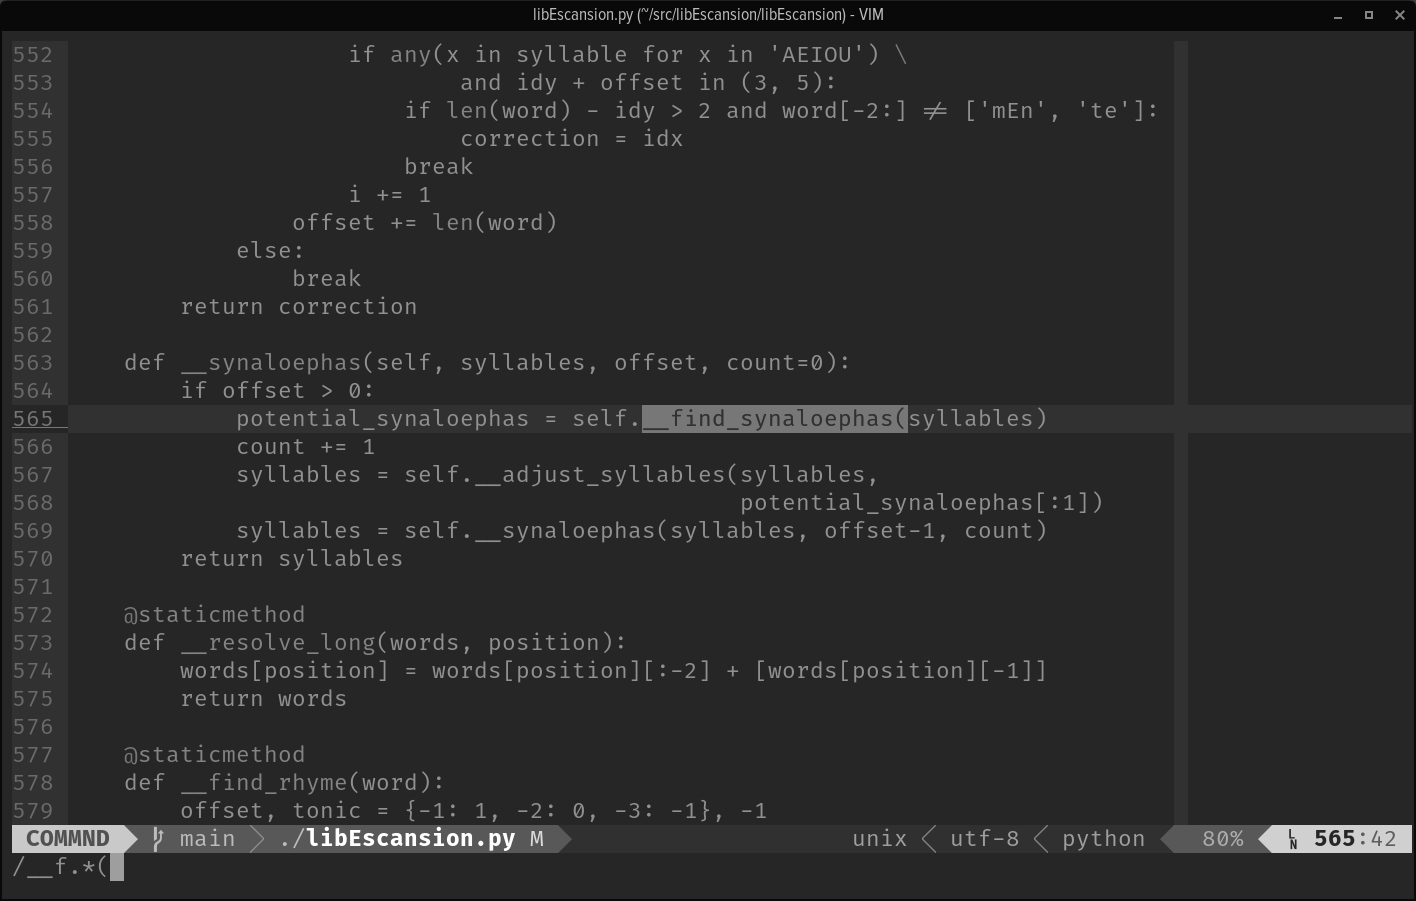
\includegraphics{images/vim.png}}
	\caption{Código Python en el editor de texto Vim.}
	\label{fig:vim}
\end{figure}

Otra cuestión a tener en cuenta es la filosofía \ac{gnu} y el software libre. Los paquetes empleados en el desarrollo de este trabajo son de código abierto y se encuentran bajo diferentes licencias libres. Esto garantiza el acceso a los programas y la libertad para usarlos sin restricciones ni coste alguno. Contra lo que podría suponerse, que los programas sean libres no compromete su calidad. Al contrario, se trata de estándares \textit{de facto} tanto en el entorno industrial como en el académico. Considérese, por ejemplo, el paquete de cálculo estadístico R\index{R} \parencite{r2019} o el propio Python en el ámbito del \textit{machine learning}\index{machine learning@\textit{machine learning}}: ambos son herramientas de uso mayoritario en su terreno.  El sistema operativo Linux, por su parte, ha demostrado su valía en aplicaciones científicas y comerciales hasta el punto de que los primeros quinientos supercomputadores más potentes del planeta operaban sobre alguna distribución de este sistema operativo\index{Linux} en noviembre de 2022 \parencite{top5002022} y domina el mercado de los servidores de internet \parencite{w3techs2023}. Creemos que nuestro trabajo, con unas exigencias mucho más modestas, bien puede aprovecharse también de estos recursos. No se trata, sin embargo, de una cuestión meramente práctica, sino que una porción sustancial del peso responde al compromiso ético con la libre difusión del conocimiento que encarna el software libre.

\begin{figure}[!ht]
	\centering\small
	\resizebox{\linewidth}{!}{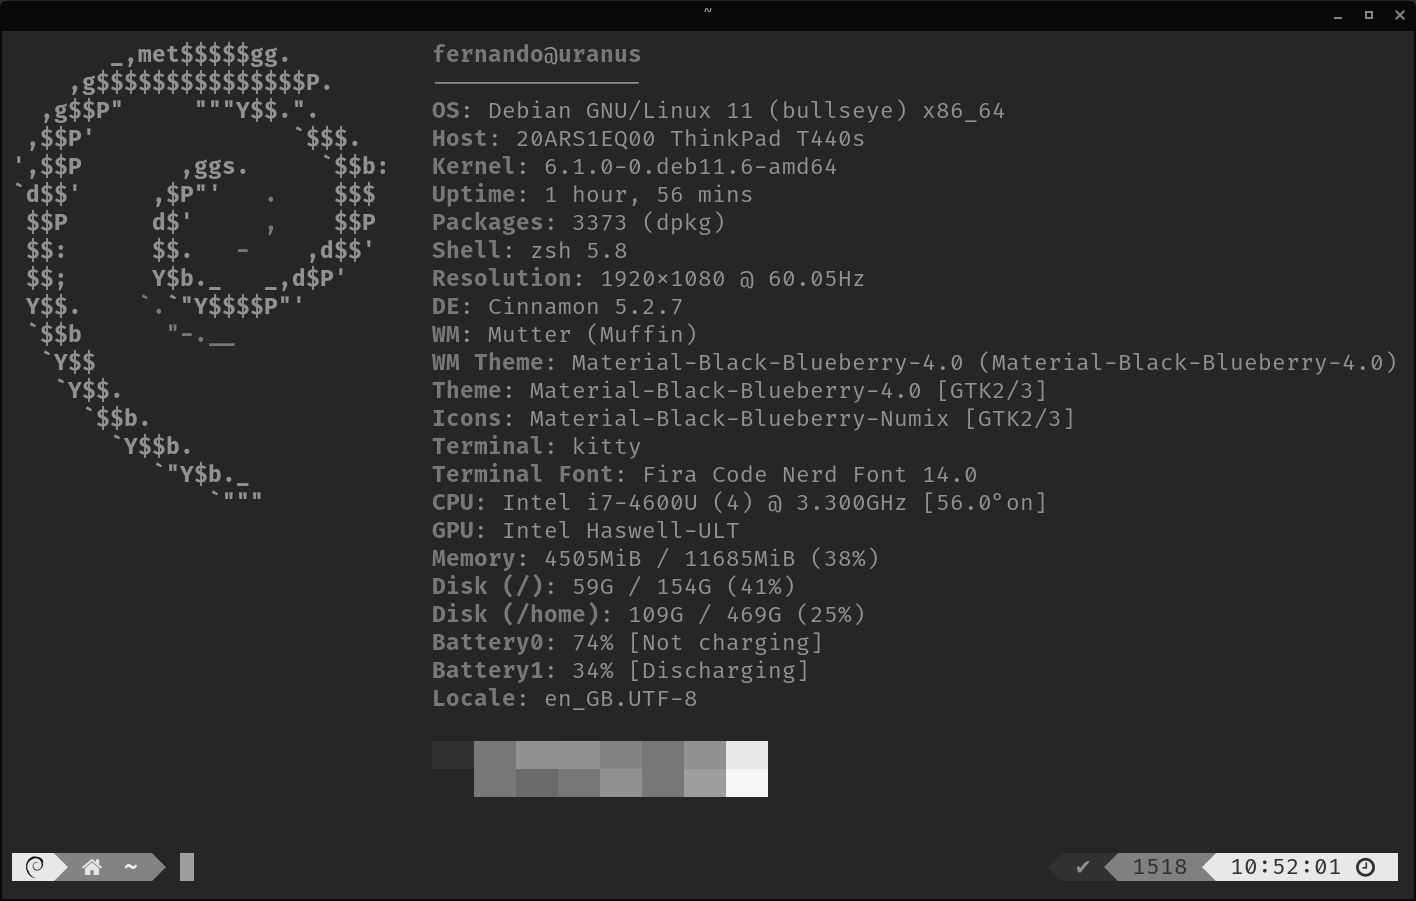
\includegraphics{images/neofetch.png}}
	\caption{Equipo de desarrollo.}
	\label{fig:neofetch}
\end{figure}

En concreto, optamos por la distribución Debian GNU/Linux\index{Linux} \parencite*{debian2022} en su versión 11 (\textit{Bullseye}), por aunar estabilidad con un completo catálogo de aplicaciones, a la vez que sigue una estricta política de licencias para seleccionar el software incluido. En cuanto al equipo físico, la mayor parte del trabajo se llevó a cabo en un Lenovo ThinkPad T440s con 12 GB de memoria RAM y un procesador de cuatro núcleos Intel CORE i7-4600U con una frecuencia de reloj de 3{,}3 GHz\footnote{Posteriormente, para procesar textos de manera masiva, encontramos que correr fragmentos del código en una GPU optimizada en lugar de la CPU del computador aceleraba sustancialmente los cálculos. Así, para la aplicación de los resultados del trabajo, empleamos los controladores comerciales de la empresa NVIDIA para poder ejecutar los programas en una tarjeta NVIDIA GeForce GTX 1060. De la misma manera, los programas completos se corrieron en diversas versiones del sistema operativo MacOS. En nuestro descargo alegaremos que, a pesar de que la portabilidad del programa deja correrlo en entornos más o menos cerrados, en su desarrollo nos ceñimos de manera estricta a software libre.} (\Cref{fig:neofetch}).


\section{Estructura del modelo}
Para plantear cómo construiremos el modelo, debemos conocer antes lo que va a hacer. En \Cref{fig:estructura} observamos una visión panorámica de los procesos que llevaremos a cabo, surgidos de depurar el concepto inicial \parencite{sanz2023a}. A grandes rasgos, tomamos los textos tal como los encontremos y los preparamos según su estructura dramática para obtener datos semiestructurados con los que el computador empiece a trabajar. No obstante, como analizaremos verso por verso, resulta más conveniente un formato que permita moverse en vertical de esta manera, por lo que tabulamos los datos y obtenemos uno estructurado. Estos datos son los que someteremos al análisis métrico, tal que la salida es una tabla con nuevas columnas para la información métrica de cada verso.

\begin{figure}[!ht]
	\centering
	\begin{tikzpicture}
	\node[datos] (input) {Datos no\\estructurados};
	\node[module, below=0.5cm of input](I1) {Preparación};
	\node[datos,right=1cm of I1] (semi) {Datos \\semiestructurados};
	\node[module, below=0.5cm of semi](I2) {Tabulación};
	\node[datos,right=1cm of I2] (est) {Datos \\estructurados};
	\node[module, below=0.5cm of est](I3) {Análisis \\métrico};
	\node[datos,right=1cm of I3] (output) {Texto \\procesado};
	
	\draw[->] (input)--(I1);
	\draw[->] (I1)--(semi);
	\draw[->] (semi)--(I2);
	\draw[->] (I2)--(est);
	\draw[->] (est)--(I3);
	\draw[->] (I3)--(output);
\end{tikzpicture}
	
	\caption{Estructura general.}
	\label{fig:estructura}
\end{figure}

En cuanto a la preparación, consta de una parte de limpieza semimanual variable, que consiste en convertir las fuentes en un formato legible para el programa y organizar el texto de acuerdo con su estructura dramática; esto lo veremos en detalle en el capítulo siguiente. En la primera parte habremos de recurrir en muchos casos a herramientas externas, mientras que la estructuración dramática se alcanza en gran medida mediante sustituciones con \textit{expresiones regulares}\footnote{Las \textit{expresiones regulares}  (abreviado \textit{\ac{regex}}, del inglés \textit{regular expression}) son una secuencia de caracteres con unas reglas sintácticas dadas que representan un patrón de búsqueda en un texto.}\index{expresión regular} una vez que el texto tiene un formato aceptable. Nos saltaremos este paso en ocasiones, siempre y cuando el texto a tratar esté ya semiestructurado, como es el caso de las ediciones en \ac{xmltei}. De cualquier forma, si los datos se hallan en un formato  adecuado, se convierten a datos estructurados de manera rápida sencilla mediante una herramienta para la manipulación automática de tablas.

Los datos tabulados resultantes son los que someteremos al análisis métrico.  Este se lleva cabo recorriendo la tabla por filas para escandir los versos uno a uno; la fila correspondiente se actualiza según los resultados con nuevas columnas.  El producto es una tabla de versos con anotaciones sobre las particularidades de cada uno en consonancia con su estructura métrica, función y jerarquía en la obra dramática.

\section{Módulos del programa}
Ya sabemos que Python cuenta con una inmensa cantidad de bibliotecas disponibles para llevar a cabo funciones comunes (y no tanto). Hemos de preguntarnos qué tareas podríamos delegar en ellas, si hay implementaciones capaces de encargarse de ello accesibles y, si es así, si estas satisfacen nuestras demandas. De lo contrario, no queda sino diseñar el procedimiento para resolver esas tareas desde cero. Como es natural, aceptaremos sin entrar en disquisiciones las bibliotecas que proveen fórmulas para llevar a cabo operaciones primitivas, esto es, aquellas que sirven para manipular tipos de datos básicos o interactuar con el sistema operativo. Nos centraremos, por el contrario, en las funciones abstractas tales como las representadas en la figura anterior. En nuestro modelo de pseudocódigo, al igual que hacemos en la implementación con el lenguaje de programación real, daremos por supuestas las funciones de tales bibliotecas y las emplearemos sintéticamente sin preocuparnos de su mecánica interna.

Por otra parte, no creamos programas para la limpieza y preparación de los datos, sino que trabajamos con herramientas preexistentes o sencillos \textit{scripts} para organizarlas, por lo que la configuración modular de los pasos más avanzados no afecta a esta etapa inicial. Los sistemas operativos de tipo Unix\index{Unix} están equipados de fábrica con potentes programas ya listos para hacer sin esfuerzo las operaciones que requerimos llevar a cabo. Los clásicos \texttt{sed} y \texttt{awk} para la manipulación de texto, por ejemplo, simplifican un tratamiento minucioso de los más pequeños detalles y admiten \ac{regex} para acotar las modificaciones. Otras herramientas facilitan los trabajos menos delicados, como convertir archivos de texto plano entre diferentes codificaciones. Incluso hay disponibles programas, como los editores de texto Vim y Emacs, capaces de hacer ambas cosas. Por lo tanto, este paso aconseja herramientas orientadas a un uso particular, más que recurrir a lenguajes de programación de uso general, sean reales, como Python, o ficticios, como nuestro pseudocódigo. Resulta mucho más sencillo resolver directamente las contingencias que surjan mediante pequeños mandatos de la línea de órdenes\index{línea de órdenes} provistos por el sistema operativo.

Una vez disponemos de los datos semiestructurados, empezaremos a automatizar realmente las tareas, ahora ya solventada la necesidad de supervisión humana. Para esto, por una parte, necesitaremos que el computador entienda el texto de entrada y, por otra, que conozca cómo estructurarlo en el formato de salida. Como veremos más adelante, tenemos previstos dos formatos semiestructurados: \ac{xmltei} y \ac{ved}, este último una notación simplificada propia para representar piezas dramáticas. Abordaremos cada uno de ellos de manera distinta. Para el primero, necesitaremos poder interpretar árboles \ac{xml} y, para el segundo, aplicar expresiones regulares\index{expresión regular} a las búsquedas. Sin embargo, entender la entrada, como decimos, es solo la mitad del trabajo. Hemos de ser también capaces de traducirla adecuadamente, por lo que necesitaremos algún tipo de herramienta que dé la posibilidad de trabajar con tablas. Las tablas, por su parte, son apenas el modo que tenemos de ordenar los versos. Una vez que hemos recorrido las líneas y llegado a la que deseamos, hay que extraer el verso de ella, escandirlo y modificar la línea mediante la adición de los valores correspondientes en nuevas columnas creadas al efecto.
 
De esta manera, si deseamos leer el texto semiestructurado, requeriremos herramientas para analizar jerarquías \ac{xml} y realizar búsquedas con expresiones regulares\index{expresión regular}. Tendremos que usar también algo que facilite la manipulación de tablas. Necesitamos, asimismo, algún instrumento para escandir versos. Para todas estas funciones existen diferentes bibliotecas disponibles listas para usar. La cuestión es: ¿debemos hacerlo? Empezaremos a responder la pregunta considerando las partes menos peliagudas.

El tratamiento de archivos \ac{xml}, la creación de un sistema de sustitución mediante expresiones regulares\index{expresión regular} y la manipulación de tablas son tareas que queremos completar, pero el modo de hacerlo es irrelevante para el propósito de este trabajo. Nos interesan los aspectos lingüísticos y literarios del análisis, no el mecanismo interno de las herramientas empleadas. Por otra parte, la escansión entra de lleno en las competencias de nuestra disciplina, así que nos ocuparemos de ella en detalle. En las pruebas de concepto, nos limitaremos a utilizar las bibliotecas estándar de Python para expresiones regulares y \ac{xml} y, para las tablas, emplearemos Pandas, por ser esta tal vez la biblioteca más popular para este tipo de tareas y, por lo tanto, de la que resulta más sencillo encontrar ayuda y documentación en caso de que se requiera. En el trabajo, obviaremos esas particularidades y asumiremos simplemente que podemos trabajar con tablas y expresiones regulares, sin entrar en cómo hacerlo.

De las bibliotecas de escansión que vimos en la revisión bibliográfica, apenas media docena se encuentran libremente disponibles. Asimismo, estas están orientadas a poemas\index{poema}, que no solo son textos monométricos, sino que además no tienen en consideración algunas irregularidades de los textos dramáticos. Esto hace necesario diseñar una herramienta de escansión específica para nuestro tipo de texto. En \Cref{fig:modulos} se esquematiza cómo se ha de llevar a cabo la escansión. Vemos que, además del conjunto de versos de entrada, tiene como salida los mismos versos ya procesados; una forma y otra se encuentran separadas por el programa encargado de análisis métrico. Dentro de este, se va recorriendo la tabla por filas para analizar los versos uno a uno; la fila correspondiente se actualiza en función de los resultados del análisis con nuevas columnas. De esta manera, escandimos cada uno de los versos y, para ello, etiquetamos gramaticalmente sus palabras para distinguir entre tónicas y átonas y hacemos la transcripción fonológica de cada palabra para trabajar con idealizaciones de sonidos y no grafemas.

\begin{figure}[!ht]
	\centering
	\begin{tikzpicture}
% Place Silabeador
\node[module] (I1) {Transcripción};
\node[module,right=0.5cm of I1] (I2) {Etiquetado\\ gramatical};
% Inner box around Items 2-3

\path (I2.north)--node[above=2mm] (arc) {Escansión} (I1.north);


\node[fit= (arc) (I1) (I2), draw, inner sep=2mm,rounded corners] (fit1) {};

\node[dato, above=1cm of fit1] (verso) {Verso};
\node[module,above=0.5cm of {verso}] (detabula) {Separación\\por verso};

% Pandas
\node[module,below=0.5cm of {fit1}] (I4) {Tabulación};
%arrow between boxes
\draw[->] (detabula)--(verso);
\draw[->] (verso)--(fit1);

\draw[->] (detabula)--(verso);
\draw[->] (verso)--(fit1);

\draw[->] (fit1)--(I4);

%upper label
%\path (fit1.north east)--node[above=15mm] (arc) {} (I4.north west);


\node[datos,left=0.5cm of verso] (Estrofas) {División\\estrófica};
\node[fit=(fit1) (I4) (detabula) (Estrofas) (I4), ,rounded corners, dashed,draw, inner sep=2mm, label={Análisis métrico}] (Overview) {};


\node[datos,left=1cm of Estrofas] (Input) {Estructura\\dramática};

\node[datos, right=0.5cm of Overview] (Output) {Texto\\procesado};



\draw[->] (Estrofas.north)|-(detabula);
\draw[->] (Input.east)|-(Estrofas);
\draw[->] (Overview.east) -- (Output.west);

\end{tikzpicture}
	
	\caption{Módulos.}
	\label{fig:modulos}
\end{figure}

Cabría cuestionar la conveniencia de delegar la transcripción y el etiquetado gramatical en bibliotecas externas. En cuanto a lo primero, se trata de una tarea compleja que requeriría, como mínimo, invertir tanto tiempo en ella como el que hemos dedicado a esta tesis. Por otra parte, existen diferentes herramientas disponibles capaces de llevar a cabo el proceso con una gran precisión. Por lo tanto, parece sensato dar un paso atrás aquí y tomar lo que se nos ofrece. En concreto, hemos optado por Stanza NLP. Se trata de una \textit{caja de herramientas}\footnote{\textit{Toolkit} en el original.} para Python de código abierto capaz de procesar más de sesenta lenguas, que incluye, entre otras funciones, la tokenización, lematización, expansión de tokens de varias palabras, etiquetado gramatical y análisis sintáctico. Dicho de otro modo, todo cuanto necesitamos. Esto lo ofrecen otros analizadores, como spaCy, pero Stanza rinde los mejores resultados para el español \parencite{qi2020}. Asimismo, se trata de un proyecto de investigación académica muy activo, por lo que el repositorio está abierto a contribuciones mediante el reporte de errores, que se resuelven en cuestión de horas. En el pseudocódigo consideramos tan solo una función genérica de \ac{pln}, lo que, recalcamos, se puede traducir de muy diversas maneras  en un lenguaje de programación, de modo que Stanza NLP es solo una posible forma de entenderlo.

El caso de la transcripción difiere del anterior. Las distintas bibliotecas para la fonología del español que hemos evaluado presentan dos problemas que desaconsejan usarlas. Por una parte, hay una dificultad de naturaleza técnica. Las bibliotecas están preparadas para transcribir exclusivamente texto con ortografía normativa, esto es, únicamente admiten los diacríticos comunes del español. Por lo tanto, no completan su labor si encuentran caracteres ajenos a esta lengua o, incluso, signos diacríticos típicos del verso, como la crema sobre vocales distintas de \textit{u}. El segundo inconveniente es conceptual: la división silábica no considera las excepciones a los diptongos ortográficos. Mientras que el primer obstáculo sería relativamente sencillo de solucionar mediante la edición del código fuente —que si es abierto, lo contempla— o la sustitución durante la preparación de los textos, el segundo requeriría una reescritura a fondo de los programas. Considerando el tiempo que habría que invertir en poner parches, estimamos que salía más a cuenta escribirlo desde cero, tomando nuestros requerimientos particulares como punto de partida y no como extras añadidos \textit{a posteriori}. Por el mismo motivo, el módulo de división silábica lo construimos también desde cero para ajustarlo a las demandas específicas de este trabajo. Esto permite, entre otras cosas, trabajar directamente con símbolos del \ac{afi} en las palabras a tratar.

En la implementación práctica nos valimos de otras bibliotecas adicionales, si bien estas resultan aún más irrelevantes para las disquisiciones de esta tesis. Entre ellas, se incluyen las dedicadas a tareas auxiliares como dibujar barras de progreso o cronometrar el tiempo de ejecución de los programas. Al ser estos elementos de control y no tener una función en el desarrollo del programa, como decimos, obviaremos tanto su uso como los motivos que llevaron a su elección.

\section{Formatos de las fuentes bibliográficas}
Para hacer las pruebas con el modelo necesitamos, huelga decirlo, textos: en particular, textos digitalizados. Hemos de dejar a un lado las condiciones ideales y enfrentarnos a las penurias del mundo real, despegarnos del \textit{texto} como idea y aproximarnos a sus realizaciones visibles. En definitiva, describiremos aquí los tipos de texto y procedencia de aquellos de los que nos hemos valido para llevar la abstracción a lo concreto.

Hay que empezar por decir que no existe un repositorio unificado de textos ni un formato estandarizado para codificarlos. Al contrario, los textos están muy repartidos y cada fuente parece tener una estructura propia, aunque superficialmente podrían antojarse similares. Los fondos semiestructurados suponen una minoría, si bien su número aumenta constantemente. Ha de tenerse en cuenta que, por lo general, el interés de la crítica se concentra en el reducidísimo conjunto de autores del parnaso canónico y, de su producción, apenas se presta atención a unas pocas obras selectas. Esto no es menos cierto en el ámbito de las humanidades digitales\index{humanidades digitales}, por lo que la probabilidad de dar con una buena digitalización de una obra menor es ciertamente escasa.

Desde el punto de vista técnico —por lo menos en lo que concierne al texto, sin entrar en cuestiones de composición y tipografía—, la labor se reduce a media decena de tipos de archivos, varios de ellos tratables con las mismas herramientas. Tenemos datos semiestructurados en \ac{xmltei} y otros no estructurados de texto, como \ac{html} y texto plano, así como también otras codificaciones más complejas, como \ac{pdf}. Asimismo, encontramos formatos para procesador de texto, como \ac{doc}\footnote{Lamentablemente, los formatos de archivo comerciales predominan sobre los abiertos, lo que, más allá de nuestro trabajo, pone trabas al intercambio de información y conocimiento cualesquiera que sean los fines.}. 

El propósito de este trabajo es, además, equipar al proyecto Sound and Meaning con una herramienta capaz de extraer datos de obras teatrales áureas e incorporar los textos junto a sus metadatos a un corpus. Este está destinado a servir como fuente para la investigación, por lo que es prioritario que los resultados de estos sean válidos. Esto obliga a restringir las fuentes según una serie de criterios que lo garanticen. Así, para hacer pruebas solo hemos tenido en cuenta las ediciones con las que trabajaba el proyecto. No debe entenderse esto como una limitación técnica, pues, en teoría, el modelo podría analizar textos que no se atuvieran a estos criterios, a pesar de que únicamente aseguraría resultados adecuados cuando aquellos se observan.

Las posibles obras candidatas para el análisis se reducen si tomamos la precaución de considerar solamente aquellas que cuentan con ortografía normalizada y modernizada. Aunque hemos intentado que los modelos sean capaces de procesar la gran mayoría de las grafías que se encuentran en las digitalizaciones de obras teatrales auriseculares, con independencia de la edición, no debemos olvidar que asumimos criterios ortográficos y fonológicos modernos. De esta manera, los resultados producidos por un texto normalizado y otro sin normalizar podrían no ser comparables debido a la imprevisibilidad del último. Es más, es posible que este tenga inconsistencias internas, lo que podría invalidar incluso un examen individual. Por lo tanto, quien haya de servirse de nuestro trabajo debería tener esto en cuenta a la hora de seleccionar las fuentes que va a usar, pues la consistencia de los análisis con ortografías no normalizadas ofrece garantías insuficientes, máxime si las convenciones de partida divergen.

La escasez de textos es aún más cierta si lo que buscamos son buenas ediciones. Lamentablemente, no todas las fuentes que se encuentran digitalizadas responden a unos criterios mínimos de calidad ecdótica. Por lo general, no presentan problemas generalizados, pero unas pocas ediciones de origen oscuro muestran deficiencias graves, alguna de ellas capaces de alterar el valor de las distribuciones de los ritmos. Por este motivo, el proyecto Sound and Meaning solo ha trabajado con textos de prestigio, pues lo contrario habría obligado a llevar a cabo un minucioso examen filológico de cada edición de procedencia no fiable para verificar su calidad; ahora multiplíquese ese tiempo por los cientos de posibles candidatos. De esta manera, aunque es probable que se hayan excluido muchos textos perfectamente válidos por carecer del aval de un editor, lo cierto es que simplifica la composición del corpus, al permitir integrar nuevos textos de inmediato. Por consiguiente, si ha de incluirse un texto de procedencia incierta, conviene tomar la precaución de examinarlo bien antes de encomendarse a los resultados de su análisis para extraer conclusiones.

Sea como fuere, con estos mimbres hay que hacer el cesto, por lo que más vale acostumbrarse a ello. En una situación óptima, dijimos, encontramos datos semiestructurados, como en el caso del corpus calderoniano  \parencite{caldracor2022}, por ejemplo. Asimismo, las obras de Artelope \parencite{oleza2022} y  T\textsuperscript{\underline{c}}/12 \parencite{tc12}, aunque no se encuentran directamente accesibles en \ac{xmltei}, aparecen como datos estructurados incrustados en el código HTML de las páginas donde se presentan las obras. Por los notables paralelismos entre las estructuras, podría sospecharse incluso que la página web se ha generado automáticamente a partir de una edición en \ac{xmltei}. Sin embargo, si bien la situación ha mejorado notablemente en la última década, siguen estando tan vigentes como entonces los \textit{desiderata} de \citeauthor{valdes2014b}~\parencite*{valdes2014b}. 

La mayoría de las fuentes de donde partimos presentan sus textos en formato \ac{pdf}. Las principales Prolope~\parencite{prolope2023} para comedias de Lope de Vega y GRISO~\parencite*{griso2020}, que dispone de una completa colección de autos sacramentales de Calderón. Esta disponibilidad, junto a los textos de CalDraCor, hace que, a día de hoy, la obra calderoniana sea posiblemente la más apta de entre sus contemporáneas para llevar a cabo estudios digitales. No podemos dejar de mencionar la Biblioteca Virtual Miguel de Cervantes \parencite{cvc2021}, aunque, en este caso, dada la diversidad de las procedencias editoriales de sus fondos, conviene seleccionar las obras individualmente.

Finalmente, tenemos obras recopiladas individualmente gracias a la generosidad del propio editor. Estas suelen encontrarse en los formatos propios de los procesadores de texto que incluyen los paquetes ofimáticos comunes. Dado que, en este caso, los textos se obtienen normalmente de forma individual e, incluso un mismo editor se vale de diversas herramientas a lo largo del tiempo —téngase en consideración que el rango temporal de estas ediciones va desde principios de la década de 1990 a textos que acaban de terminarse y aún no están publicados\footnote{Prolope, Instituto de Teatro Clásico de Almagro,  comedias.org y CANON60, entre otras.}—, estas ediciones son tremendamente heterogéneas.  Dada esta variedad de procedencias, nos enfrentamos a diferentes obstáculos para preparar los textos de manera que podamos emplearlos directamente en el computador.

\section{Diferencias entre textos, textos y textos}
La heterogeneidad de los textos requiere aproximarse individualmente a los problemas que presenta cada uno de ellos. No solo nos hallamos ante una plétora de formatos incompatibles entre sí, sino que, incluso, encontramos diferencias en la manera en que se codifican dos textos en el mismo formato. La diferencia principal estriba en que algunos de esos formatos proveen facilidades para la manipulación y análisis textual; otros, por el contrario, suponen un obstáculo que, en ocasiones, resulta insalvable.

El primero de los retos que uno se encuentra para tratar un texto digitalizado —y no por obvio deja de ser el más importante— es obtener el susodicho texto. Aquí se distinguen varias tipologías: por una parte, los textos accesibles públicamente y, por otro, aquellos que no lo están y han de obtenerse a través de diversas vías, como el préstamo o la compra. Estos textos, con independencia de cómo se hayan conseguido, pueden ser libres o tener restricciones legales o técnicas. Esto es, hay textos que prohíben la manipulación y copia en cumplimiento de los derechos de autor, lo que se fuerza en ocasiones mediante la aplicación de un sistema de protección digital anticopia. No obstante, se encuentran textos de dominio público con la misma protección, lo que también impediría tratar un texto, aunque fuera perfectamente legítimo.

Asumiremos que trabajaremos legalmente con los textos de los que disponemos y que estos no están restringidos por protección digital alguna. Los formatos más comunes son \ac{pdf}, TXT, \ac{xml} y cualquiera de los tipos de archivos privados e incompatibles entre sí —incluso entre diferentes versiones de supuestamente el mismo programa— de los diversos procesadores de texto\footnote{En el curso de los trabajos llevados a cabo para el proyecto Sound and Meaning, pudo comprobarse que, lamentablemente, los archivos creados con un procesador de textos suelen estar en alguno de los diferentes formatos cerrados de Microsoft Office; excepcionalmente, aparece algún archivo en Open Document Format (\ac{odf}). Como anécdota, algunas de las obras del corpus del proyecto estaban compuestas con WordPerfect 5.2, una versión del programa salida al mercado en 1992; aunque los procesadores de texto comerciales modernos fueron incapaces de reconocer ese formato, el paquete ofimático libre LibreOffice.org no tuvo problema para abrirlo.}. Una vez se dispone de acceso al archivo, el objetivo es convertirlo a datos semiestructurados. En el caso de \ac{xml}, se obvia ese paso porque ya lo está.

\section{Peor escenario: PDF}
Los archivos \ac{pdf} albergan el texto completo, pero este no es directamente accesible. No se trata de un texto plano ni de un lenguaje de marcado como \ac{xml}, sino de una descripción de las páginas. Para poder verlo, requerimos de la mediación de un programa capaz de interpretar el código binario del archivo y representarlo de manera visual en la pantalla. Se presenta el problema de que, de esta forma, no hay posibilidad de trasladar la composición de la página directamente y, por lo tanto, tampoco la estructura de la obra. Se necesita convertir ese documento a texto plano y, a la vez, preservar el mayor número de elementos visuales posible, de manera que se minimice el trabajo manual. La forma de hacerlo dependerá de como se haya compuesto el archivo, ya que esto determina el modo en que se codifica el texto.

Cada una de las páginas contiene bloques de instrucciones que definen segmentos de contenidos y sus características. En el caso de los bloques de texto, estos suelen estar repartidos de acuerdo no a un criterio textual, sino a las necesidades de la maquetación. Por ejemplo, para representar \textit{Ejemplo}, ubicaría la \textit{E} en la posición $(x,y)$  y el segmento \textit{jemplo} en $(x+1-n, y)$, de modo que desplazaría el segundo segmento $n$ puntos hacia la izquierda para hacer un acoplamiento parecido a \textit{Ej}, en lugar de conservar el espaciado como en \textit{E\strut j} \parencite{glyph2022}. Esto hace que los programas para la extracción automática del texto aborden la tarea colocándolo en orden de lectura sin más. La complejidad de la maquetación y su proximidad a la jerarquía textual son determinantes para decidir la manera de abordar el texto.

Si la maquetación del documento se aviene hasta cierto punto a la estructura textual, recurriremos a herramientas de conversión de formato como \texttt{pdftotext}, que dan la opción de conservar la distribución espacial de  los elementos en la página, aunque no consigan un resultado perfecto.  Después, el trabajo consistiría en afinar esta conversión mediante expresiones regulares\index{expresión regular}. De esta forma,  se eliminan cabeceras de página, numeración de los versos múltiplo de cinco y aparato crítico, así como las voladas de llamada a nota si las hubiera. Esta parte no presenta muchas dificultades, ya que los saltos de página vienen marcados con un metacarácter.

Sabemos que la primera línea tras el salto de página es la cabecera, por lo que se elimina. Los números de verso aparecen a la derecha del texto, precediendo de manera inmediata al final de línea y después de uno o más espacios o tabuladores que los separan del texto. Sabiendo esto, suprimimos los guarismos que cumplan esas condiciones, ya que no encontraremos un equivalente textual. No suele haber llamadas a nota porque la numeración se corresponde con el número de verso. Si las hubiera, no obstante, esto tampoco presentaría excesivo problema, ya que las llamadas van anejas a una palabra o a un signo de puntuación no precedido por un guarismo y, en este último caso, seguidas de espacio. Aunque, hipotéticamente, podrían darse casos como \textit{123\textsuperscript{1}}, los guarismos intratextuales son prácticamente inexistentes, por lo que asumimos simplemente que varios de ellos a final de línea son cifras del mismo número.

Las notas a pie de página, sin embargo, admiten el tratamiento directo  con dificultad. Sabemos que entre las notas y el cuerpo textual hay varias líneas de espaciado, a semejanza de la composición del texto de origen. Desafortunadamente, esto no se da siempre ni todas las veces que lo hace indica la separación entre ambas entidades. Con la numeración de las notas sucede lo mismo: da una pista, pero no es ni necesaria ni suficiente. La segunda línea y subsiguientes de una nota de más de un renglón no van precedidas de un guarismo, como tampoco lo van la continuación en la siguiente página de una nota extensa. Por otra parte, cuando alternan varios personajes genéricos del mismo tipo, estos se nombran a veces simplemente mediante sus ordinales, como \textit{1.º}, \textit{2.º}, etc., por lo que, aparte de la numeración a principio de línea, se requieren otros criterios. Un tercer indicio es la longitud de la línea, si bien aquí también encontramos tanto parlamentos en prosa de líneas largas como notas tan cortas como un verso de arte menor. La combinación de estos criterios no es una garantía lógica de los aciertos, si bien, en la práctica, es suficiente. Así, buscaremos líneas largas antes del final de página que estén separadas por varios espacios del cuerpo principal y líneas largas que comiencen por un número y las siguientes hasta el final de la página.

El cuerpo del texto no es uniforme. Por una parte, las líneas\index{línea} y las didascalias de personaje\index{didascalia de personaje} suelen presentar pocas dificultades porque el sangrado revela la función y este se conserva al convertir entre formatos. Hay, empero, dos elementos textuales que requieren una inspección visual detenida: las acotaciones\footnote{Trataremos la didascalia de personaje como un elemento distinto al resto de acotaciones, pues estas tendrán entidad propia, mientras que aquella proporcionará un atributo.} y los versos compartidos. Las acotaciones\index{acotación}, salvo que vayan centradas en la página, no se distinguen de otros componentes textuales porque el texto plano no tiene la capacidad de aplicar formato a los caracteres. Por lo tanto, los fragmentos en cursiva del archivo \ac{pdf} de origen se traducirían en redonda en el de texto plano. Esto hace inevitable el marcado manual. Las continuaciones de versos compartidos, por su parte, se ven o no dependiendo de si el espaciado original es suficiente como para que la herramienta de conversión lo interprete como tal. Un espaciado insuficiente implica que en el archivo de texto no habrá distinción en el sangrado de un verso normal y la continuación de un verso compartido. Si bien suelen encontrarse fallos en la segunda parte del verso, a partir de la tercera, al llevar dos niveles de sangrado, resulta más infrecuente. En cualquier caso, conviene hacer un examen manual para marcar estos versos. El proceso consiste en un primer cotejo visual para buscar últimos versos de un parlamento y primeros del siguiente más cortos que los del bloque les rodea. Una vez localizados, se verifica que ambas líneas componen un solo verso y se ajusta el sangrado si procede.

Puede darse la situación de que un archivo  \ac{pdf} con una estructura interna compleja produzca unos resultados tan pobres s al convertirlo tratando de conservar la maquetación, que requiera tal cantidad de correcciones manuales que se dispare el tiempo necesario para preparar el texto. En algunos de estos casos, es posible usar una alternativa geométrica. Ahora emplearíamos otra herramienta para convertir a lenguaje de marcado, tal como \texttt{pdftohtml}, para traducir el archivo \ac{pdf} a \ac{xml}. El resultado no se trataría de un \ac{xml} como en la jerarquía definida por \ac{tei}, sino que los elementos se caracterizarán por su posición espacial. Estos poseen atributos que indican mediante pares de coordenadas su ubicación física en la página. Con esto en mente, estimamos los rangos en los que comienzan los elementos horizontalmente en cada página. Es importante porque, además de variar la maquetación en general entre páginas pares e impares, hay elementos que no aparecen en todas las páginas. Así, los fragmentos centrados incrementarían el rango, cuyo punto de inicio sería la mitad de cuerpo de texto para un solo carácter. Lo mismo sucede con las continuaciones de versos compartidos, cuya posición inicial depende de la longitud de la parte precedente del verso en la línea o líneas anteriores.  Por el desplazamiento vertical sabemos a qué línea corresponden los segmentos. Sea como fuere, ya es factible aproximar con cierta exactitud la distribución de los elementos y pasar el \ac{xml} a texto. A pesar de ser un método más engorroso que el anterior, presenta al menos una ventaja sobre aquel, en tanto que se conservan los atributos de los caracteres, con lo que se encuentran las acotaciones con más facilidad. No resulta esta tampoco una solución infalible porque, por ejemplo, una expresión latina intercalada a comienzo de verso sería indistinguible de una acotación interna como \textit{Canta} si esta última no va entre paréntesis.

La carga de temporal de este tipo de conversiones es variable, pero el coste por obra ($C$) es inversamente proporcional al número total de obras ($n$), en tanto que se requiere invertir una cantidad notable de tiempo ($T_0$) para establecer reglas que evalúen los patrones de la primera y aplicarlas a cada una de las siguientes ($i$) de manera mecánica, lo que toma una pequeña cantidad de tiempo ($t$) en comparación con el necesario para encontrarlas.  

\begin{equation}\label{eq:tiempo}
C = \frac{T_0 + \sum_{i=0}^{n} t_i}{n},\: t_i \ll T
\end{equation}

En términos llanos, esto es que, si disponemos de varios archivos con la misma estructura interna, solo tenemos que encontrar las reglas en uno de ellos y, una vez con ellas, podemos aplicarlas en bloque al resto de textos. Por lo tanto, cuantos más fuentes de la misma procedencia obren en nuestro poder, más eficiente en tiempo será convertir cada uno de ellas. Por el contrario, el peor escenario en términos de efectividad sería tratar una obra suelta. En el caso del corpus de \textit{Sound and Meaning}, casi un centenar de archivos PDF procedían de las digitalizaciones del GRISO \parencite*{griso2020} de autos calderonianos. Todos ellos respondían al mismo modelo y pudieron ser tratados mediante la conversión directa a texto plano. Esto hizo posible crear un corpus de varios cientos de obras a pesar de partir de \ac{pdf}.

\section{Escenario regular: archivos ofimáticos}
Con archivos ofimáticos nos referimos a aquellos formatos producidos por el programa de edición de textos de un paquete para trabajos de oficina, como Write de LibreOffice.org o Word de Microsoft. Nos encontramos con estos archivos sobre todo en casos en los que el propio editor de la obra se la ha facilitado al proyecto \textit{Sound and Meaning}. La manera de codificar el texto con formato varía sustancialmente; oscila entre estándares abiertos como \ac{odf}, que internamente usan archivos \ac{xml} comprimidos, y cerrados diseñados específicamente para mantener un mercado cautivo, como es el caso del formato \ac{doc} de Microsoft y su plétora de versiones y revisiones apenas parcialmente compatibles, incluso entre sí. En cualquier caso, una vez conseguimos abrirlos mediante el programa correspondiente, trabajaremos con ellos sin complicaciones, ya que no requerimos recurrir a las extensiones propias más esotéricas, sino simplemente algunas funciones elementales para manipular texto con formato. En concreto, tienen importancia la alineación del párrafo, las sangrías y algunas propiedades de los caracteres (cursiva y versalitas, sobre todo). El objetivo es convertir a texto plano marcando de alguna manera esas propiedades para poder conservarlas.

Los elementos que afectan al párrafo y la línea se marcan atendiendo  a su espaciado. No es así con las propiedades de los caracteres, ya que estos pueden ir intercalados entre otros sin formato adicional. De este modo, marcaremos estos con una etiqueta reconocible, esto es, una serie de caracteres que no se vayan a dar en el texto. Si bien esto añade artefactos al formato, reconocerlos y tratarlos como tales es trivial, por lo que las ventajas superan con creces los inconvenientes, que son de orden estético en cualquier caso. 

Para este trabajo, nos hemos servido del paquete LibreOffice.org porque da la posibilidad de buscar y reemplazar mediante la combinación de expresiones regulares\index{expresión regular} estandarizadas y elementos de formato, por lo que los pasos que lo requieren pueden darse fácilmente. La extensión \textit{Alternative Find \& Replace for Writer} hace posible otras sustituciones. Las alternativas existentes, como Microsoft Office, ofrecen herramientas con una funcionalidad restringida en comparación. Así pues, optamos por la alternativa libre.

\begin{figure}[!ht]
	\centering\small
	\resizebox{\linewidth}{!}{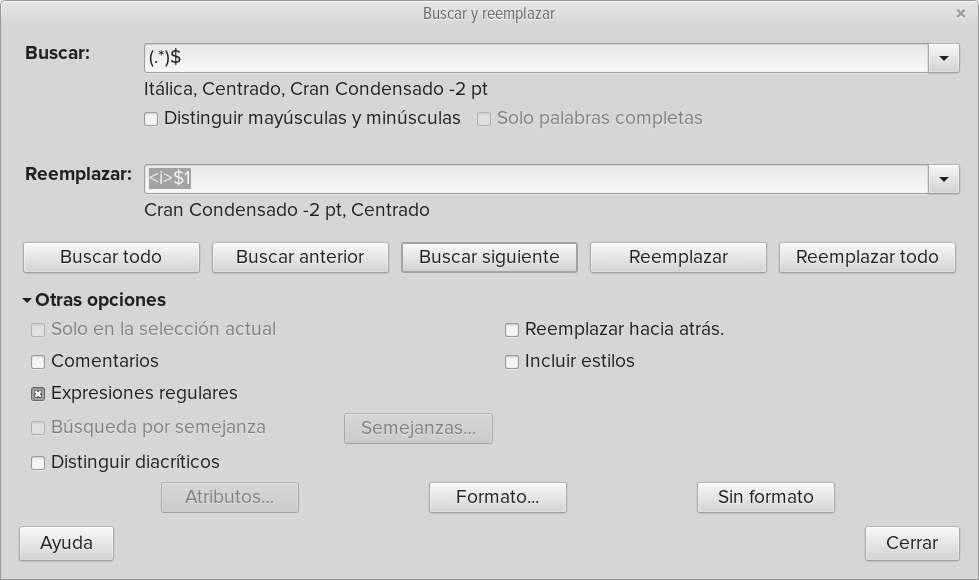
\includegraphics{images/searchandreplace.png}}
	\caption{Diálogo de búsqueda de LibreOffice.org.}
	\label{fig:searchandreplace}
\end{figure}	

Esta opción haría hipotéticamente posible salvar el texto en formato \ac{odt} y escribir un pequeño programa que llevara a cabo la preparación procesando el código \ac{xml} después de descomprimirlo. Al ser pocos los archivos en este formato, resulta más práctico tratarlos de forma manual. El inconveniente es que esto obliga a abordarlos de uno en uno, por lo que, de haber una cantidad grande de estos, convendría considerar procesar automáticamente el código \ac{xml}. De cualquier manera, conviene restringir las sustituciones desde el procesador de textos ofimático a aquellas que no puedan resolverse sencillamente en el archivo de texto con la línea de órdenes\index{línea de órdenes} del sistema operativo, ya que el tratamiento individual de los archivos acarrea un alto coste temporal.

\begin{figure}[!ht]
	\centering\small
	\resizebox{\linewidth}{!}{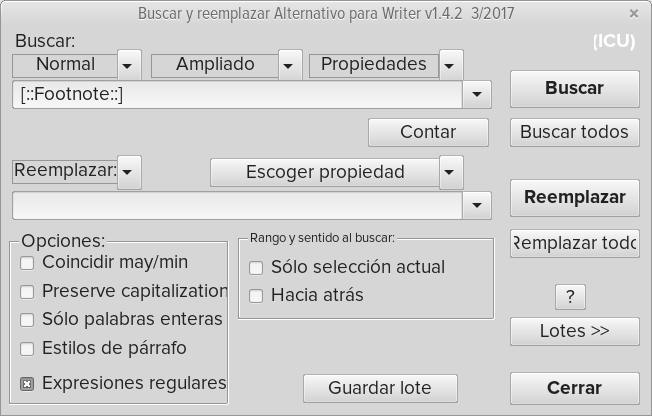
\includegraphics{images/asearchandreplace.png}}
	\caption{Extensión de búsqueda \emph{Alternative Find \& Replace for Writer}.}
	\label{fig:asearchandreplace}
\end{figure}

Para las sustituciones en el cuerpo del texto, se selecciona \texttt{Buscar y reemplazar}, que se encuentra en el menú \texttt{Editar}. Esto abre un diálogo con diferentes opciones para nuestro propósito (\Cref{fig:searchandreplace}). Aquí debe marcarse la casilla correspondiente para habilitar el uso de expresiones regulares\index{expresión regular}, y empezar a hacer las sustituciones requeridas. La expresión de la ilustración, por ejemplo, buscaría y capturaría (paréntesis) cualquier cadena de texto (\texttt{.*}) hasta el final de la línea ($\$$), siempre que la línea esté centrada y el texto en cursiva. Sustituiría el texto por el patrón capturado (todo hasta el final de la línea), pero, por ejemplo, con la cadena \texttt{<i>} antepuesta\footnote{La elección no es casual, sino que se aviene a las etiquetas del formato \ac{ved}, que veremos más en detalle algunas páginas más adelante.}, de modo que se identificaría esta línea una vez perdida la alineación y las propiedades del tipo de letra. Al pulsar \texttt{Reemplazar todo}, se aplicaría al texto completo. Sabemos también que los versos están alineados a la izquierda, mientras que el texto en prosa suele ir justificado a ambos lados de la página. Esto se aplica para buscar esta característica y marcar los pasajes necesarios.

Por su parte, para eliminar bloques paratextuales, también en el menú \texttt{Editar} seleccionaremos el elemento \texttt{Alt. buscar y reemplazer}\footnote{La errata está en el menú de la barra de tareas.}~[\textit{sic}]. Esto abre otro diálogo con opciones parecidas a la búsqueda estándar, aunque algo diferente (\Cref{fig:asearchandreplace}). Aquí también marcaremos la casilla que activa el uso de expresiones regulares\index{expresión regular}. En este caso, no buscaremos cadenas de texto, sino bloques (notas a pie de página, al final, etc.). Dejaremos vacío el campo con la sustitución, pues así indicaremos que el bloque buscado ha de reemplazarse por un elemento vacío. De esta manera, la expresión del ejemplo, eliminaría todo el cuerpo de notas a pie de página.

Los diferentes niveles de sangrado se indican mediante tabuladores, tantos como niveles haya. El espaciado interior también es de utilidad, ya que nos valdremos de él para diferenciar entre unidades estructurales. Una separación de un solo espacio divide componentes de una misma unidad, mientras que un número mayor de espacios vacíos indica una separación de otra índole. De esta manera, distinguiremos entre didascalia de personaje y parlamento con independencia de las propiedades del texto. El ejemplo \ref{ex:loctext} capturaría en un primer grupo la didascalia de personaje y en otro el parlamento, de manera que podríamos alterarlos de la manera más conveniente.

\begin{exe}
	\ex\label{ex:loctext}\texttt{\^{}\textbackslash s*(\textbackslash S+(?:\textbackslash s\textbackslash S+)*)(\textbackslash s\{2,\})(\textbackslash S+)\$}
\end{exe}

Podríamos modificar la expresión regular sustituyendo \texttt{\^{}\textbackslash s*}, que denota la presencia de cero o más (\texttt{*}) espacios (\texttt{\textbackslash s}), por un rango de entre $i$ y $j$ espacios, por ejemplo con \texttt{\^{}\textbackslash s\{$i$,$j$\}}, de manera que encontraríamos la presencia de versos compartidos. Así, adaptaríamos estas expresiones a los casos particulares y, de igual forma, abordaríamos el archivo de texto resultante.

\section{Escenario óptimo: XML-TEI}
El mejor caso posible es la conversión desde un archivo \ac{xmltei}. Este presenta todos los elementos necesarios para producir una forma estructurada y sin ambigüedades. El esquema de \Cref{fig:xmltei} muestra una descripción de la estructura básica de una obra de teatro, como las que se encuentran, por ejemplo, en DraCor. De la raíz \texttt{<TEI>} cuelgan dos ramas. La primera es \texttt{<TeiHeader>} es una cabecera de metadatos. La segunda es \texttt{<text>}, con el texto propiamente dicho, como se observa en el esquema de la jerarquía \ac{xmltei} (\Cref{fig:xmltei}). El estándar \ac{tei} define un detallado conjunto de etiquetas, cuyas directrices se extienden a lo largo de casi dos mil páginas en su última versión \parencite{tei2022}, por lo que aquí solo nos ocuparemos sucintamente de aquello que afecta directamente al análisis y, aun así, de manera muy superficial.
	
	\begin{figure}[!ht]
		\begin{forest}
			forked edges,
			%for tree={%
				%	edge path={\noexpand\path[\forestoption{edge}] (\forestOve{\forestove{@parent}}{name}.parent anchor) -- +(0,-12pt)-| (\forestove{name}.child anchor)\forestoption{edge label};}
				%}
			%forked edges,
			for tree={
				align=center,
				font=\tiny,
				%anchor = west,
				grow'=0, % tree direction
				%edge={->,>=latex},
				parent anchor=east, child anchor=west, % edge anchors
				%rounded corners, draw,
				text height=0.5ex, text depth=0.2ex % <<<<<<<<<<<<<
			}
			[\texttt{<TEI>}
			[\texttt{<teiHeader>}
			[\texttt{<fileDesc>}
			[\texttt{<titleStmt>}
			[\texttt{<title>}]
			[\texttt{<author>}]
			]
			[\texttt{<publicationStmt>}
			[\texttt{<authority>}]
			[\texttt{<publisher>}]
			[\texttt{<date>}]
			[\texttt{<availability>}
			[\texttt{<licence>}]
			]
			]
			[\texttt{<sourceDesc>}
			[\texttt{<bibl>}]
			[\texttt{<date>}]
			[\texttt{<idno>}]
			]
			]
			[\texttt{<particDesc>}
			[\texttt{<listPerson>}
			[\texttt{<person>}]
			[\texttt{<personGrp>}]
			[\texttt{...}]		
			]
			]
			[\texttt{<TextClass>}]
			]
			[\texttt{<text>}
			[\texttt{<front>}
			[\texttt{<castList>}
			[\texttt{<head>}]
			[\texttt{<castItem>}]
			[\texttt{...}]
			]
			]
			[\texttt{<body>}
			[\texttt{<div>}
			[\texttt{...>}
			[\texttt{<sp>}
			[\texttt{<speaker>}]
			[\texttt{<l>}]
			[\texttt{<stage>}]]
			[\texttt{...}]
			[\texttt{<stage>}]
			]
			[\texttt{...}]
			]
			[\texttt{...}]
			]
			]
			]
		\end{forest}
		\caption{Estructura de XML-TEI.}
		\label{fig:xmltei}
	\end{figure}

De la cabecera cuelgan otras subestructuras. En \texttt{<fileDesc>} hay información sobre la edición. Tal vez la más relevante de estas ramas sea \texttt{<titleStmt>}, pues incluye el título y el autor. Aquí se usan varias etiquetas, añadiendo argumentos si es necesario, como, por ejemplo, \texttt{<title type"main">} y \texttt{<title type"subtitle">}, para reflejar el título principal y el subtítulo, o crear una subsestructura en  \texttt{<author>} especificando detalles como nombre o apellidos. Los datos de la publicación cuelgan de \texttt{<publicationStmt>}, como la organización responsable de  la edición, en \texttt{<authority>}, la editorial en \texttt{<publisher>}, la fecha en \texttt{<date>} y la disponibilidad \texttt{<availibility>}, donde caben etiquetas como \texttt{<licence>} para expresar los términos legales de uso del texto (\ref{ex:publicationStmt}). Los datos de la obra original están bajo \texttt{<sourceDesc>}, con diversos identificadores, así como la fecha.

\begin{exe}
	\ex\label{ex:publicationStmt}\begin{lstlisting}[language=xml,upquote=true,numbers=none]
<publicationStmt>
    <authority>University of Vienna,Institute of Romance Languages and Literatures</authority>
    <publisher xml:id=""/>
    <date when="2022-01-12">
        <time when="14:08:57"/>
    </date>
    <idno type="quadramaX">La siembra del Señor (Los obreros del señor)</idno>
    <availability>
        <licence>
            <ab>CC-BY 4.0</ab>
            <ref target="https://creativecommons.org/licenses/by/4.0/">
                Licence
            </ref>
        </licence>
    </availability>
</publicationStmt>
\end{lstlisting}\end{exe}

Resulta de la mayor importancia la rama \texttt{<particDesc>}, ya que en ella se configura la lista de personajes que intervienen en la obra. Esta lista consta de una entrada única de tipo \texttt{<person>} para cada personaje\index{personaje} o, en el caso de personajes colectivos, de tipo \texttt{<personGrp>}, como ilustra el ejemplo \ref{ex:xmlid}. Asimismo, cada personaje se caracteriza más en detalle mediante atributos de la etiqueta, entre los cuales consideraremos dos. Tenemos, por ejemplo, \texttt{sex}, que se emplea para denotar si el personaje es masculino, femenino o lo que convenga. Otros atributos similares se emplean de manera análoga. Tanto o posiblemente más relevante para el tratamiento digital que los atributos de clase, es el identificador, pues asigna a cada uno de ellos un código individual que se mantiene a lo largo de la obra. Esto simplifica seguir a cada personaje, con independencia de que se referencia a un mismo locutor con diferentes didascalias, como abreviaturas, títulos de cortesía o, incluso, que un personaje cambie de nombre a mitad de la obra. Para ello, además de la didascalia bajo la etiqueta \texttt{<speaker>}, disponemos de un indicador paratextual \texttt{xml:id} único para cada personaje, siempre el mismo con independencia de la didascalia con que se nombre. De esta forma, una vez que hemos definido \texttt{xml:id="scipion"}, cada uno de los parlamentos del personaje llevará ese identificador, escríbase la didascalia \textsc{Scipión} o \textsc{Scip.}.  De esta manera, los versos bajo ambas se reconocen de forma sencilla como pertenecientes a un mismo personaje \textit{Scipión}.
\begin{exe}
\ex\label{ex:xmlid}\begin{lstlisting}[language=xml,upquote=true,numbers=none]
<person sex="MALE" xml:id="scipion">
    <persName>SCIPIÓN</persName>
</person>
<personGrp sex="UNKNOWN" xml:id="musicos">
    <persName>MÚSICOS</persName>
</personGrp>
\end{lstlisting}\end{exe}

Pueden existir más ramas de este árbol, algunas de las cuales resultan extremadamente útiles para facilitar la clasificación de la obra, como, por ejemplo, \texttt{<textClass>} (\ref{ex:textclass}). 

\begin{exe}
	\ex\label{ex:textclass}\begin{lstlisting}[language=xml,upquote=true,numbers=none]
<textClass>
	<keywords>
		</person>
		<term type="genreTitle">Comedia</term>
		<term type="subgenreTitle">De capa y espada</term>
	</keywords>
</textClass>
\end{lstlisting}\end{exe}

Respecto a los datos de la cabecera, cuantos más se encuentren a nuestra disposición, tantas más serán las posibilidades en lo concerniente al análisis del texto y en lo que atañe a cuestiones de archivo. Resulta evidente que la inclusión de la fecha inicial de la publicación, datos de los personajes\index{personaje} o del género de la obra permite cruzar esa información para buscar patrones. Pero no menos importantes son otras cuestiones, como la licencia de uso, que condicionará la manera de emplear los datos, o los identificadores de la obra y el autor, que facilitan la búsqueda y clasificación de esta. Las ediciones usadas proporcionan toda la información requerida, pero la cuestión podría cobrar importancia con fuentes menos minuciosas.

La rama \texttt{<text>} contiene el texto propiamente dicho, con dos partes denominadas \texttt{<front>} y \texttt{<body>}. Esta rama tiene la particularidad de que los contenidos de las etiquetas se muestran en el texto, por lo que los metadatos han de señalarse como atributos de la etiqueta. Bajo \texttt{<front>}, del ingleś \textit{front matter}, tendríamos, en principio, los preliminares. Sin embargo, en nuestro caso, aquí se incluye también el elenco bajo una estructura \texttt{<castList>} que contiene elementos del tipo \texttt{<castItem>} y \texttt{<head>}, este último para una cabecera del tipo «Personajes que hablan» o «\textit{Dramatis personae}».

La rama \texttt{<body>} se divide en partes bajo la etiqueta \texttt{<div>}. Aquí es habitual especificar el tipo y la numeración, cuando es necesario, para poder encontrar ramas bajo la etiqueta, como en \texttt{<div type="act" n="1">}. Bajo estas, puede haber asimismo subdivisiones, en la que, en lugar de \texttt{type="act"}, aparece, por ejemplo, \texttt{type="scene"} y, por lo general, especificando también la numeración. Finalmente, en la rama \texttt{<div>} más profunda, se encuentra el texto de la obra.

Este texto\footnote{Se trata de una codificación propia a partir de una edición todavía inédita de Ignacio Arellano del auto calderoniano \textit{La exaltación de la Cruz}.} tiene dos tipos principales de etiqueta, \texttt{<stage>} y \texttt{<sp>} (\ref{ex:parlamentos}). La primera señala las acotaciones\index{acotación} y la segunda los parlamentos. En estos últimos, además de la parte correspondiente al texto, debe tenerse muy en cuenta el atributo  \texttt{who} de la etiqueta, que es el identificador único que se había definido en la cabecera y que permite, por ejemplo, encontrar redes de relaciones entre personajes\index{personaje}. Es preferible usar este identificador en lugar de la etiqueta \texttt{<SPEAKER>}, ya que esta se refiere a la didascalia y no al locutor, por lo que, como indicamos, pude variar, lo que dificultaría su seguimiento. La última etiqueta que nos interesa es \texttt{<l>}, que marca cada línea.

Además del atributo \texttt{n} que, como los elementos anteriores, denota la numeración, puede aparecer el atributo \texttt{part}. Este sirve para indicar el comienzo de un verso (\texttt{"I"}), su continuación (\texttt{"M"}) y su término (\texttt{"F"}), para identificar versos distribuidos a lo largo de dos o más líneas. Podría darse el caso de que, en lugar de la etiqueta \texttt{<l>}, halláramos otra del tipo \texttt{<p>}. Esta denotaría que no encierra una línea de parlamento, sino un párrafo y, por lo tanto, prosa. Se emplea, por ejemplo, cuando un personaje lee una carta. Tampoco es raro que, inmediatamente bajo \texttt{<sp>}, no se abra un bloque mediante una etiquetas de tipo \texttt{<l>}, sino que sea una estructura intermedia \texttt{<lg>} y, por debajo de esta, se encontrarían las líneas. Por ejemplo, \texttt{<lg type="stanza">}. Las acotaciones internas se representan mediante etiquetas \texttt{<stage>} dentro de una estructura \texttt{<sp>}, en lugar de a su mismo nivel como las externas.


\begin{exe}
	\ex\label{ex:parlamentos}\begin{lstlisting}[language=xml,upquote=true,numbers=none]
<sp who="#morlaco">
    <speaker>MORLACO</speaker>
    <l met= "+-++-++--+-" rhyme="ina">¿Yo beldad? Loco me es sobre gallina</l>
    <l part="I">este príncipe.</l>
</sp>
<sp who="#siroes">
    <speaker>SIROES</speaker>
    <l part="M">¿Dónde...</l>
</sp>
<sp who="#morlaco">
    <speaker>MORLACO</speaker>
    <l part="F" met="+-+--+-+++-" rhyme="ada">No sé nada</l>
    <l n="1665" met="+--+++-+-+-" rhyme="ada">y hágase allá, que es burla muy pesada.</l>
</sp>
\end{lstlisting}\end{exe}

Cabe la posibilidad de incluir atributos \texttt{met} para el patrón rítmico y \texttt{rhyme} para la rima. No resulta común encontrarlo en textos españoles y, de hecho, no hemos hallado ninguna edición que lo incluya, aunque sea bastante habitual en lenguas clásicas, el griego sobre todo. Así que, si de bien poco sirve tener la posibilidad en el análisis careciendo de textos que hagan uso de ella, la recordaremos para aprovecharla más adelante y reflejar los resultados de nuestros análisis.

Conociendo la estructura, la extracción de datos resulta trivial: recorremos recursivamente las subestructuras de \ac{xmltei}  hasta llegar al nivel más profundo de cada rama, leemos los datos que en ella se encuentran y los tratamos de la manera que resulte más conveniente. Por ejemplo, para tratar los parlamentos procederemos como en \Cref{list:xml2txt}.

\begin{algorithm}[!ht] %or another one check
	\caption{Conversión de XML-TEI a texto.}\label{list:xml2txt}
%	\Ffuncion{\Reordena{tei2txt}}{
%		\cuerpo \gets\ \texttt{<body>} \;
%		\actos \gets\ cuerpo.encuentra(\texttt{<div>}) \;
		\ForEach{$acto \in\:actos$}{
			\ForEach{$escena \in\:acto$}{
				\ForEach{$estructura \in\:escena$}{
					\If{$estructura\: \is\: parlamento$}{
						\ForEach{$l\acute{\imath}nea \in\:estructura$}{
							\If{$(\neg\:part\:\vee part = \langle F\rangle)$}{
								\guardaverso{$anteriores + l\acute{\imath}nea$} \;
								anteriores \gets $\emptyset$
							}
							\Else{anteriores \gets $anteriores + l\acute{\imath}nea$}
						}
					}
					\Else{\guardaac{estructura}}
				}
			}
		}
\end{algorithm}

El algoritmo consiste en recorrer los actos, y en cada uno de ellos —supondremos que no hay escenas ni otros niveles intermedios—, recorremos a su vez las estructuras inferiores, como los parlamentos y acotaciones. Aquí se bifurca el flujo de datos según el tipo de estructura. Si es un parlamento, lo recorremos línea a línea. Primero probamos si la línea se corresponde a un verso, comprobando que la línea no lleva atributo de parte o es la sección terminal de un verso. En este caso, procesaremos las partes anteriores del verso —que será un elemento nulo de no ser un verso compartido—, seguidas de esta línea y reiniciamos la variable intermedia donde guardamos los elementos anteriores. Si la línea no es terminal, vamos añadiendo las nuevas partes del verso a la variable intermedia. Si, por el contrario, la estructura no es un parlamento, la procesaremos como acotación\index{acotación}. De manera análoga, haremos lo propio con todos los elementos de la cabecera, aunque, en ese caso, los terminales serán normalmente de un solo tipo —con excepciones como la descripción de los personajes\index{personaje}— y no hará falta recorrer en un bucle, sino buscar determinados elementos únicos.

\section{Precauciones con la codificación}
Hasta aquí hemos visto las estructuras de datos como meras abstracciones. Sin embargo, a la hora de trabajar en la práctica con ellas, debemos observar ciertas precauciones de índole más técnica que conceptual, ya que estamos sujetos a la representación interna de los caracteres del texto empleada por el computador. Incluso cuando el procedimiento empleado por todos los archivos de texto es muy similar, hay algunas diferencias en la codificación que son susceptibles de causar dificultades y errores. En nuestro trabajo, esto redunda tanto en la organización de los textos como en la manera de tratar las fuentes. Para entender el problema nos remontaremos a los primeros estándares de codificación informática de texto.

En las computadoras personales típicas, el máximo común divisor es  \textit{American Standard Code for Information Interchange} básico, más conocido por sus siglas \ac{ascii} \parencite{wells1997}. Este estándar surgió a principios de la década de 1960 a expensas de la American Standard Association. Se diseñó con el objetivo de representar textos escritos en inglés y, más específicamente, de la variedad americana de esta lengua. Por este motivo, no era capaz de mostrar caracteres ajenos a ese alfabeto, como los que emplean muchas lenguas europeas, el español entre ellas. La cantidad de caracteres no alfanuméricos también estaba limitada y, por ejemplo, no preveía el uso de símbolos monetarios distintos del dólar estadounidense. Como es de suponer, otros sistemas de escrituras no basados en el alfabeto latino quedaban totalmente excluidos. Este \ac{ascii} se representa mediante 7 bits, por lo que hay un máximo de $2^7$ combinaciones, que se reparten entre 95 \textit{caracteres}\index{carácter} imprimibles\index{carácter!imprimible} y 33 de control\index{carácter!de control}\footnote{Un carácter no equivale necesariamente a un grafema\index{grafema}, sino a un patrón de bits al que le corresponde un significado. Este admite diferentes formas: puede ser gráfico —una letra, un signo, un símbolo o un espacio en blanco—, en cuyo caso hablaremos de caracteres imprimibles, pero también puede representar una acción no visible —borrar el carácter anterior o marcar el final de una línea—, y hablaremos de caracteres de control \parencite[139]{haralambous2019}.} en su revisión más moderna \parencite[423-433]{mackenzie1980}. 

Esta codificación es precisamente la que usa el \textit{Speech Assessment Methods Phonetic Alphabet} (\ac{sampa}). Se trata de un alfabeto que se desarrolló en el marco del proyecto European Strategic Programme on Research in Information Technology (\ac{esprit}) de la Comunidad Económica Europea para representar en soporte informático la fonología de lenguas europeas occidentales. Una de las premisas de su diseño era que debía garantizar la compatibilidad con las computadoras de la época. De acuerdo con esto, podríamos valernos de ella para representar las transcripciones fonológicas. Sin embargo, esto presentaría problemas para los fragmentos grafémicos.

Debido a las limitaciones de \ac{ascii}, diversos fabricantes y organizaciones concibieron sus propios métodos de codificar los caracteres extendidos, entre los que se encuentran las letras con diacrítico y muchos de los signos de puntuación que necesitamos para escribir en español. Así, encontramos que la \ac{iso} propuso su estándar ISO-8859-1 y Microsoft desarrolló Windows-1252 para las lenguas europeas. Ambos son de 1 byte, lo que son suficientes para representar $2^8$ combinaciones o, lo que es lo mismo, 256 caracteres.

Hoy en día, hemos superado aquellas constricciones impuestas por la técnica, podemos representar en texto plano no solo todas las grafías que demanda una correcta ortotipografía en cualquier lengua europea, sino muchos más caracteres. El desarrollo de las computadoras personales hizo irrelevantes las limitaciones que prevenían la aparición de nuevos sistemas de codificación. \textit{Unicode}\index{Unicode} se presentó en 1991 con la idea de ofrecer una solución a las constricciones de las  codificaciones existentes y, especialmente, para dar soporte a todas las lenguas vivas y muertas, así como otros sistemas de símbolos cuya inclusión estuviera justificada. Cada carácter Unicode tiene el mismo número de bits, por lo que todos ellos se codifican como un único carácter para cada grafema, tanto del español como del \ac{afi}. Por defecto, Unicode emplea dos bytes para representar un solo carácter, esto es, dieciséis bits. Esto permite usar un total de $2^{16}$ o, lo que es lo mismo, 65{.}536 caracteres \parencite{bettels1993}. Los sistemas operativos modernos de tipo Unix\index{Unix} más extendidos —Linux\index{Linux} y MacOS\index{MacOS}— soportan Unicode\index{Unicode} de forma nativa en prácticamente todas sus versiones posteriores al año 2000. De esta manera, no resulta ya necesario emplear \ac{sampa}, pues pueden representarse con la misma codificación tanto los textos grafémicos españoles como su transcripción al \ac{afi}.

Esto no solo simplifica la comprensión del texto, ya que la notación de los programas se corresponde con la impresa, sino que tiene implicaciones en el análisis informático de los textos transcritos. En concreto, la limitación del número de caracteres disponibles obliga a que SAMPA represente dígrafos y ligaturas mediante dos caracteres, mientras que Unicode los representa con uno. Por ejemplo, SAMPA obligaría a preprocesar el fonema /\texttoptiebar{tʃ}/ al representarlo con los caracteres ASCII \textit{t} y \textit{S}, como \textit{tS}. Unicode, por su parte, aúna los símbolos del \ac{afi} \textit{t} y \textit{ʃ} mediante un único carácter digrafémico \textsc{\textit{ʧ}}. De esta manera, se vuelve innecesario crear una excepción para tratar este sonido africado\index{consonante!africada}, al poder representarse como una única unidad.

Aunque el formato final de nuestros datos está codificado según Unicode\index{Unicode}, esto no implica necesariamente que los archivos de origen también opten por el mismo sistema. Por lo tanto, hay que convertir aquellos archivos de texto que partan de codificaciones distintas. En el caso de \ac{ascii}, no sería necesario porque es un subconjunto de Unicode\index{Unicode}; desafortunadamente, como ya dijimos, es un subconjunto que no incluye todos los diacríticos y signos ortográficos necesarios para escribir en español de acuerdo con su ortografía, por lo que ningún texto aceptado va a estar en \ac{ascii} puro. Las otras aproximaciones de un byte a la representación de caracteres extendidos provocan serios problemas, pues producen artefactos que alteran el texto (\Cref{fig:codificacion}). Si bien los signos ortográficos no afectarían a nuestro propósito, los diacríticos supondrían un problema grave. Por lo tanto, se hace necesario unificar formatos en algún momento y, por razones prácticas, lo haremos cuanto antes. 

\begin{figure}[!ht]
	\centering
	\footnotesize
	\begin{subfigure}{.5\textwidth}
		\texttt{¡Oíd, mortales, oíd,\\
			y al pregón de la Fama\\
			todos acudid!}
	\end{subfigure}%
	\begin{subfigure}{.40\textwidth}
		\texttt{¡Oà d, mortales, oà d,\\
			y al pregón de la Fama\\
			todos acudid!}
	\end{subfigure}
	\caption{Transliteración de la variante ASCII ISO-8859-15 a Unicode.}
	\label{fig:codificacion}
	\normalsize
\end{figure}

La solución pasa por identificar de antemano el tipo de codificación y convertir el archivo a Unicode\index{Unicode}. Esto no presenta mayor problema en un entorno Unix\index{Unix}, cuyas herramientas proveen soluciones simples. Mediante el mandato \texttt{file} identificamos la codificación del archivo y, utilizando un programa al efecto\footnote{Por poner dos ejemplos de entre los empleados, la biblioteca \ac{gnu} C de Linux\index{Linux} provee \texttt{iconv} y MacOS\index{MacOS} dispone de \texttt{textutil} para la tarea.}, solventamos el inconveniente.

 A pesar de que Unicode es la opción que mejor se adapta a nuestro propósito, tampoco está exenta por completo de algunas fuentes potenciales de complicaciones. Una de ellas, que debemos señalar para poder evitarla, deriva del propio diseño de la codificación.  Aunque esta se adecúa a las ortografías de las lenguas más conocidas y es capaz de representar un gran número de caracteres, soluciona las combinaciones de dos maneras diferentes, indistinguibles para el ojo, pero no precisamente triviales de tratar digitalmente de manera elegante. Para representar un carácter compuesto, pongamos por ejemplo la letra eñe minúscula, se usa la codificación Unicode\index{Unicode} simple \textsc{latin small letter n with tilde}. Esta es el carácter U+00F1 para el computador y, para nosotros, el grafema \textlangle{}ñ\textrangle. También existe la posibilidad de representarlo mediante la combinación de los caracteres \textsc{latin small letter n} \textlangle{}n\textrangle{} y \textsc{combining tilde} \textlangle$\tilde{\text{\DVS◌}}$\textrangle. En este último caso, aunque nosotros veríamos igualmente el grafema \textlangle{}ñ\textrangle{} en la pantalla, el computador leería la secuencia U+006E U+0303: esto es, dos caracteres. Como dijimos, hasta aquí no sería problema para atenerse a la ortografía española. Desafortunadamente, no puede decirse lo mismo de otros sistemas de representación. 

Concretamente, las vocales no silábicas, marcadas con un símbolo diacrítico de breve invertida inferior \textlangle\textsubarch{{\DVS◌}}\textrangle, solo admiten representación en Unicode mediante una combinación, de forma que hemos de tratarlo como dos caracteres \parencite[17]{moran2018}. Por esta razón, ante la dicotomía de introducir excepciones en el código por una cuestión técnica visual o mantener la fidelidad a los principios rectores, optamos por lo segundo, dando primacía a la claridad conceptual del proceso sobre la estética del resultado\footnote{Dejamos abierto para  futuras versiones de la biblioteca modificar esto.}. De este modo, representaremos las semivocales /\textsubarch{i}/ y /\textsubarch{u}/ con el mismo símbolo que las semiconsonantes /j/ y /w/, respectivamente\index{semivocal}\index{semiconsonante}\index{vocoide}, y usaremos el carácter individual con diacrítico de breve integrado (\textlangle{ă}\textrangle, \textlangle{ĕ}\textrangle{} y \textlangle{ŏ}\textrangle) para el resto de vocoides.

La codificación de los símbolos que señalan acentos primarios o secundarios en las sílabas  (ˈ, ˌ) no se ven afectados gracias a que, al contrario que los modificadores diacríticos, estos anteceden a la sílaba que modifican. Por consiguiente, cuando aparece uno, se tiene en cuenta como modificador, pero se ignora para lo demás \textit{a priori}.

Otro problema que se plantea son las distintas formas en las que los diferentes sistemas representan el final de línea (\textsc{lf}) y el retorno de carro  (\textsc{cr}). Las máquinas con un sistema operativo de tipo Unix\index{Unix} —GNU/Linux\index{Linux} y MacOS\index{MacOS}, por ejemplo—, emplean únicamente \textsc{lf}. Por su parte, los computadores Windows\index{Windows} usan \textsc{cr} \textsc{lf}, mientras que sistemas Apple antiguos emplean \textsc{cr}. Esto supone para nosotros que, cuando abrimos un texto con saltos de línea para Windows, veremos al final de cada fila un artefacto correspondiente al carácter \textsc{cr}, sin uso en nuestro sistema. En un texto creado en una máquina Apple antigua, lo que aparecerá será tan solo una larga línea con artefactos dispuestos a intervalos, ya que no tenemos el carácter \textsc{lf} que indica el final de la línea, pero sí \textsc{cr}, para el que no encontramos uso.  Por esta razón, es necesario convertir aquellos textos que así lo requieran. De nuevo, usaremos la herramienta estándar de Unix \texttt{file} para identificar el tipo de final de línea que tenemos y programas específicos para convertir las marcas de un sistema a otro\footnote{Bajo Linux\index{Linux}, \texttt{mac2unix} o \texttt{dos2unix} o \texttt{textutil} en MacOS\index{MacOS}. Se puede hacer usando tan solo las herramientas estándar de Unix\index{Unix}, como \texttt{sed} o \texttt{awk}.}.

Una vez podemos manipular las fuentes para tratar el texto con la asistencia del computador, nos hallamos en condiciones de empezar a identificar y clasificar las entidades que requerimos para caracterizar la obra teatral. En realidad, como veremos en el capítulo siguiente, la cuestión no es tanto encontrar estos elementos, pues ya hemos visto que la codificación \ac{xmltei} ha resuelto este reto y proporciona un buen modelo, sino seleccionar aquellos componentes que necesitemos, así como encontrar una disposición que facilite los análisis cuantitativos. 
\label{chap:6}
				\chapter{Estructura digital del texto dramático}\label{chap:B2}
\epigraphhead[50]{\epigraph{Quédese vusté con Dios,\\
		ya no salgo a la comedia\\
		y ya me voy a mi casa,\\
		porque no quiere el poeta\\
		que le haga estorbo el gracioso\\
		cuando hay un paso de veras.}{Rojas Zorrilla, \textit{Peligrar en los remedios}}}
\section{Texto dramático, datos dramétricos}
En este capítulo retomamos lo visto sobre los datos y las diferentes formas de usarlos para ser aplicados a las entidades dramáticas. El objetivo ahora es definir estas como estructuras de datos, sea como elementos singulares o mediante las relaciones entre ellos. Damos por supuesto que, tras seguir lo expuesto en el capítulo anterior, disponemos ya de textos \textit{limpios} y preparados para trabajar digitalmente de modo automático.

Si bien el formato \ac{xmltei} se presta perfectamente a almacenar información y da facilidades para su manipulación, su estructura jerárquica requiere un paso intermedio para el tratamiento estadístico. Los paquetes de mayor difusión en la academia y la industria trabajan con marcos de datos\footnote{{\textit{Data frame}} en inglés.}, que no son otra cosa que una vía de abstracción para representar la sempiterna tabla. Esto es, una serie de elementos distribuidos a lo largo de filas, cuyas características se definen en columnas. De esta manera, si queremos conocer la característica $j$ del elemento $i$, nos desplazaremos verticalmente hasta la fila $i$-ésima y, en ella, miraremos el contenido de la celda correspondiente a la columna $j$-ésima.

Esto naturalmente requiere conocer en primer lugar qué características cuantificaremos para definir el formato de la tabla. También hemos de saber cómo se representarán esas características para asignarles un valor numérico o categórico, de lo que depende el formato del valor de la celda. Asimismo, necesitamos conocer qué elementos poseedores de tales características observaremos. De esta manera, nos interesa definir las entidades que constituyen la forma externa del texto dramático para poder estructurarlas después en forma tabular.

Como dijimos, estas entidades y sus relaciones estaban indicadas explícitamente en los archivos en \ac{xmltei}. Lamentablemente, no todas las fuentes se encuentran disponibles en este formato ni todas lo que lo están son fiables \parencite{valdes2014b}. Podríamos codificarlos nosotros mismos —de hecho lo haremos más adelante—, pero estaríamos en la misma tesitura porque, para hacerlo, debemos identificar primero los elementos textuales y sus relaciones.

La solución por las que nos inclinamos pasa por un sistema de tratamiento de textos semimanual. Esto es, los textos de origen se limpian primero mediante los procesos  semiautomatizados presentados en el capítulo anterior, si bien, en lugar de dejarlos tal cual, aprovechamos para que el proceso los organice según ciertas convenciones que nos resulten más convenientes. El formato nos ha de permitir identificar las entidades textuales sin ambigüedades para luego automatizar su tratamiento. Proponemos un sistema de codificación de textos dramáticos que hemos denominado Visually-Encoded Drama (\ac{ved}) para alcanzar este propósito. Hemos desarrollado este formato específicamente para el proyecto \textit{Sound and Meaning} como una aportación extra al limpiado de los textos. Esto es, surgió como una evolución de la preparación directa de los archivos, aquella consistente en eliminar información metatextual como encabezados, paginación o aparato crítico. Con unos cambios mínimos, que apenas requieren operaciones adicionales más que adaptar las ya usadas al nuevo objetivo, el texto resultante puede proporcionar información adicional sobre su estructura, así como metadatos relevantes. 

\section{De texto plano a VED}
La manipulación de las fuentes plantea varias necesidades. Por una parte, hay que disponer de un formato de representación de las ontologías propias del drama. Por otro lado, crearlo a partir del formato de partida debe implicar la mínima intervención manual. Además, todo ello debería poderse llevar a cabo sin conocimientos técnicos. De ahí el carácter visual del formato que ideamos. Este reproduce la disposición de los elementos estructurales que se hallan en la página, de manera que, al menos los concernientes al texto, pueden codificarse sin necesidad de aprendizaje (\ref{ex:vedmin}).

\begin{lstlisting}[frame=none,numbers=none,caption={Ejemplo mínimo de codificación VED.},label={ex:vedmin}]
UNO
	Es el primer verso de Uno,
	y este es uno...
OTRO
		...compartido.
	y este lo dice solo Otro.
\end{lstlisting}

Resulta evidente la similitud con el formato que encontramos en cualquier edición moderna, si bien la didascalia de personaje\index{didascalia de personaje} toma una línea\index{línea} para ella sola. Naturalmente, esta información es insuficiente, por lo que hemos de añadir otros datos de alguna manera. Nos valdremos para ello de etiquetas simples, pero siempre respetando la estructura visual del texto. Dada la flexibilidad que ofrece esta codificación, resulta sencillo construir herramientas para traducir este formato a otros, como \ac{xmltei}, por lo que también las hemos construido para llevar a cabo esta tarea. Por ahora, empezaremos por describir el formato \ac{ved} y, a continuación, explicaremos cómo llegamos hasta él.

El formato \ac{ved} está concebido con la idea de que sea intuitivo. Por lo tanto, nada mejor para explicarlo que con un ejemplo. Vemos elementos que reproducen la forma arriba descrita, así como otros menos obvios, por estar precedidos de marcas de control.  Aquí tenemos dos tipos: por un lado, etiquetas, que se asemejan a las usadas en \ac{html} o \ac{xml}, aunque, al contrario que esas codificaciones, no van por pares con una etiqueta para abrir y otra para cerrar, ya que no cumplen esa función. Al establecer una relación biunívoca entre entidad y línea, los límites de esta son los de aquella. La etiqueta, pues, solo se utiliza a efectos clasificatorios.

\begin{lstlisting}[frame=none,numbers=none,caption={Ejemplo de archivo VED.},label={ex:ved}]
<x>Comentario
<a>Autor
<t>Título
<tt>Subtítulo
<g>Género
<gg>Subgénero
<o>Obtenido de la edición tal*https://foo.bar/fuente
<f>1600-1699
<el>PERSONAS QUE HABLAN EN ELLA|Uno*Otro, otro personaje*UN TERCERO
<j>Primera Jornada
<i>Acotación
UNO #uno
	El primer verso de Uno,
	segundo, de Uno, el verso.
	Tercero es medio.
OTRO #otro
		que
UNO #uno
			sigue
	en este otro parlamento.
	<i>Acotación interna.
	Quinto verso, también fin.
UNO Y OTRO #uno \#otro
	<e>¡Fin!
<i>Vanse. Acotación externa. Entra un tercero.
TERCERO #tercero
	<i>Lee.
	<p>Esto no es un verso sino un texto en prosa.
\end{lstlisting}

Como su nombre indica, el formato \ac{ved} reproduce la estructura espacial de la pieza teatral. Se trata de un simple archivo en texto plano —por lo tanto, puede ser abierto y editado directamente en cualquier sistema sin necesidad de instalar programas adicionales—. Cada elemento textual se representa en una línea\index{línea}; estas líneas se configuran de manera interna de diferentes formas para marcar su función en el texto. Los parlamentos\index{parlamento} se distinguen de las didascalias de personaje\index{didascalias de personaje} mediante el sangrado, mientras que otras características del texto, así como el resto de acotaciones\index{acotación}, elementos textuales dramáticos inusuales y metadatos se indican mediante un reducido conjunto de etiquetas. Esto resulta en una composición legible directamente, pero semiestructurada, que se procesa automáticamente con un programa específico. Por otra parte, al remedar la disposición sobre el papel, este sistema es muy intuitivo, por lo que apenas requiere unos minutos para poder empezar a preparar textos.

Al comienzo, vemos una serie de líneas\index{línea} sin sangrar y con una etiqueta que recuerda a las que se emplean en \ac{html}. Su función es, sin embargo, un poco diferente, ya que no indica atributos sino categorías. La etiqueta \texttt{<x>} la usamos para añadir comentarios que no han de ser tenidos en cuenta en el análisis. Resulta útil cuando hay que introducir advertencias o aportar información adicional necesaria para el desarrollo del trabajo. El nombre del autor lo señalamos con la etiqueta \texttt{<a>}. Si estamos codificando la obra para procesarla e incorporarla a un corpus, sería importante convenir una forma estandarizada, de manera que varias obras del mismo autor no aparezcan con distintas variantes del nombre; el computador es incapaz de notar algo aparentemente obvio como que tanto \texttt{Calderón} como \texttt{Calderón de la Barca} y \texttt{Pedro Calderón de la Barca}, o incluso \texttt{Calderón de la Barca, Pedro}, son formas de nombrar a la misma persona. En la práctica, hemos optado por emplear versiones abreviadas del nombre en la codificación y recurrir a una tabla de conversión externa para sustituirla por el nombre completo. Aquí, confiaremos en el sentido común del lector.

Las etiquetas \texttt{<t>} y \texttt{<tt>} corresponden al título de la obra y a su subtítulo, respectivamente. La fecha la introducimos tras la etiqueta \texttt{<f>}. En el caso normal, indicamos la fecha mediante un año representado por cuatro guarismos arábigos. Si no conocemos la fecha concreta, optaremos entre usar un rango mediante dos años separados por un guion o una fecha insegura, que indicamos con un año y un signo de cierre de interrogación. Cualquier otro formato sería válido, pero, dado que no es posible contemplar todas las variantes posibles, al convertirlo a \ac{tei} produciría un formato de fecha no estandarizado. Asimismo, para dejar constancia de la procedencia editorial de la fuente, empleamos la etiqueta \texttt{<o>}. Aquí incluiremos cuantos datos estimemos convenientes y, de manera opcional, 
 una dirección de una página web asociada introducida por un asterisco. Este campo no se encuentra estandarizado, ya que no está concebido por ahora para ser estudiado, sino con fines de archivo y clasificación. Volvemos aquí a la cuestión ontológica: ¿son los datos editoriales de la edición moderna entidades susceptibles de ser estudiadas mediante la lectura distante\index{lectura distante}? Dada la falta de publicaciones que así lo consideren, lo dejaremos por ahora como un dato estrictamente metatextual no cuantificable; tal vez, habría que revisar este punto en el futuro y normalizar el formato para poder tenerlo en consideración como una variable más. 

El género y el subgénero se indican mediante \texttt{<g>} y \texttt{<gg>}. Aquí debemos considerar la misma precaución que observamos con el nombre del autor, porque el computador sería incapaz de reconocer, por ejemplo, \texttt{capa y espada} como equivalente a \texttt{de capa y espada} sin complicar el algoritmo de evaluación de los términos a comparar. Una solución eficaz consiste en asignar códigos mnemotécnicos sencillos para cada género y escribir luego de manera automática el nombre completo usando una tabla de conversión.

Tenemos además la  etiqueta \texttt{<el>} con la que introducimos el elenco. Aquí pondremos opcionalmente la cabecera que utiliza la obra para introducirlo (por ejemplo, «\textsc{Personajes que intervienen}») seguida de una barra vertical y, a continuación, los personajes. Estos van separados por asteriscos e, internamente, puede constar, además del nombre, de un epíteto opcional si lo hubiera, introducido por una coma. Conviene cuidar el detalle aquí, porque esta línea\index{línea} la emplearemos en la conversión a \ac{xmltei} no solo para los metadatos, sino para presentar las partes impresas en el cuerpo del texto. En efecto, la información necesaria para producir el bloque del cuerpo textual bajo la rama \texttt{<front>} la obtenemos a partir de la información proporcionada en estos metadatos. Gracias a ella disponemos del autor, los títulos y las \textit{dramatis personae}.

La etiqueta \texttt{<j>} señala un nuevo acto\index{acto} o jornada\index{jornada|see {acto}}. La aplicaremos incluso en obras sin macrodivisiones, pues su primera ocurrencia es la marca que señala el comienzo de la parte estructural de la obra. No existe una etiqueta específica para señalar las escenas porque no es habitual que este tipo de segmentación se señale explícitamente en las obras. A partir de aquí, comienza la representación en sí y señalamos la jerarquía estructural del texto mediante el espaciado.

Dejamos las didascalias de personaje en una línea\index{línea} sin sangrar y sin etiqueta que introduzca el texto. Podemos, además, señalar facultativamente el identificador \texttt{<xml:id>} de cada personaje para que se tenga en consideración  al convertirlo a \ac{tei}. Esto puede resultar útil cuando aparecen parlamentos\index{parlamento} colectivos, para indicar con ello quiénes toman parte. En cualquier caso, poniendo el nombre de un personaje, hemos señalado el comienzo de un nuevo parlamento. Ahora  sangraremos el texto para todo el bloque de orden jerárquico inferior supeditado a la intervención de este personaje, que incluye tanto texto como acotaciones internas\index{acotación}. Podemos encontrar versos completos o comienzos de verso\index{verso}, que no necesitan más información, ecos, que indicaremos con la etiqueta \texttt{<e>} o fragmentos en prosa, que denotamos mediante la etiqueta \texttt{<p>}. De la misma manera, si queremos señalar una acotación interna, lo indicaremos sangrando la línea antes de etiquetarla con \texttt{<i>}; para una externa, evitaríamos el sangrado. En el caso de versos compartidos, la continuación o continuaciones de un verso inconcluso se marcan con unidades de sangrado adicional para que reproduzca visualmente la edición impresa. En la práctica, dos unidades de sangrado son suficientes para el computador, pero es recomendable emplear niveles sucesivos, ya que estos ayudan a la identificación visual. Su equivalente en \ac{xmltei} lo vemos en \Cref{extendedchars:xmlved3}.

\begin{lstlisting}[frame=none,numbers=none,caption={Equivalente \ac{xmltei}.},language=xml, label={extendedchars:xmlved3}]
<sp who="#uno">
    <speaker>UNO</speaker>
    <lg>
        <l>El primer verso de Uno,</l>
        <l>segundo, de Uno, el verso.</l>
        <l part="I" >Tercero es medio.</l>
    </lg>
</sp>
<sp who="#otro">
    <speaker>OTRO</speaker>
    <lg><l part="M">que</l></lg>
</sp>
<sp who="#uno">
    <speaker>UNO</speaker>
    <lg>
        <l part="F">sigue</l>
        <l n="5">es este otro parlamento.</l>
        <stage>Acotación interna.</stage>
        <l>Quinto verso, también fin.</l>
    </lg>
</sp>
<sp who="#uno #otro">
    <speaker>UNO y OTRO</speaker>
    <lg><l>¡Fin!</l></lg>
</sp>
<stage>Vanse. Acotación externa. Entra un Tercero.</stage>
<sp who="#tercero">
    <speaker>TERCERO</speaker>
    <stage>Lee.</stage>
    <p>Esto no es un verso sino un texto en prosa</p>
</sp>
\end{lstlisting}

De esta manera, ya tendríamos nuestro texto como datos semiestructurados, lo que nos permitiría tratarlo con el computador para todo tipo de estudios cuantitativos sobre las entidades definidas. Asimismo, el formato facilitaría otras aproximaciones. Pensemos, por ejemplo, en una prueba estilométrica clásica, en la que la entidad medida es la frecuencia de las palabras. En este caso, no hemos definido esa entidad para su medición, aunque hacerlo llevaría muy pocos pasos y, además, sencillos. Considerando que los programas de estilometría toman el texto en sí como entrada, deberíamos eliminar tanto los elementos paratextuales (título de la jornada) como aquellos otros no dramatizados (acotaciones\index{acotación}...). Bastaría para esto aplicar una serie de expresiones regulares\index{expresión regular} para eliminar secuencialmente los elementos deseados. Empezaríamos, por ejemplo, por todas las líneas\index{línea} sin sangrar\index{sangrado}, luego las que empiezan con una etiqueta de acotación y, finalmente, a discreción de quien lleve a cabo la prueba, tal vez las líneas introducidas por etiquetas de prosa o eco.

\begin{lstlisting}[frame=none,numbers=none,caption={Preparación de archivo VED para análisis estilométrico.},language=bash, label={extendedchars:sed}]
	4> sed '/^\S/d' pieza.ved | sed '/<i>.*/d | sed 's/<.*>//'	 
\end{lstlisting}

Podríamos llevar una cuenta de personajes en escena según un procedimiento análogo al de determinar personajes colectivos. La aproximación más simple es incluirlos en una lista a medida que intervienen. La distribución de esta cambiaría con cada intervención, de manera que el último personaje pasaría a ocupar siempre la posición final. De esta forma, tras una acotación \textit{vase}, se sabría exactamente a quién alude. Más complicado sería \textit{Vanse}, porque atañe al menos a dos personajes, pero desconocemos a cuántos en concreto. Aproximaríamos aquí, dejando el resto a la revisión manual. Si se especifican nombres en la acotación, esta afectaría a los aludidos sin importar la posición que ocupen.  Lo vemos en \Cref{list:vanse}, donde evaluamos una lista $fuera$ indica los personajes en escena por orden de salida y la acotación. 

\begin{algorithm}[!ht]
	\caption{Personajes que se van.}\label{list:vanse}
	\Fmetodo{\EnEscena{fuera, acotación}}{
		\If{`Va[n]se' $\in$ acotación}{
			\If{$\exists personaje_i \in acotaci\acute{o}n, \forall personaje \in fuera$}{
				\fuera \gets $fuera - personaje_i$
			}
		}
		\ElseIf{`Vase' $\in$ acotación}{
			\fuera \gets $fuera_{1..n-1}$
		}
		\ElseIf{`Vanse' $\in$ acotación}{
			\fuera \gets $fuera_{1..n-2}$
		}
		\Return{fuera}	
	}
\end{algorithm}

En nuestro caso, hemos usado el procedimiento para determinar los personajes colectivos (\Cref{list2:txt2tei}), de manera que si aparece, por ejemplo, \textsc{Las dos}, serán los dos últimos personajes femeninos que han precedido la última intervención, o, si es todos, —de modo algo impreciso—, la lista entera salvo el personaje que acaba de hablar. Sin embargo, bastaría con utilizar ese valor para otros propósitos, como los descritos en \Cref{chap:ejdram} si así se desea. 

\section{Excurso \Roman{excurso}: De VED a XML-TEI}\stepcounter{excurso}
Como hemos visto, el formato \ac{ved} define una ontología que constituye un subconjunto de \ac{xmltei} y permite representar las principales entidades textuales definidas por este último para el drama. Esto facilita emplear los archivos \ac{ved} para codificar una obra y convertir la edición automáticamente a \ac{xmltei} de manera rápida, incluso sin estar familiarizado con ninguno de ambos formatos. Para llevar a cabo este proceso de transformar datos semiestructurados de forma visual en otro jerárquico no estrictamente secuencial, emplearemos el programa \texttt{text2tei} \parencite{sanz2022sc}, cuyo código fuente se encuentra en \Cref{list2:txt2tei} en su última versión a la fecha de entrega de este trabajo. Su mecanismo, a grandes rasgos, consiste en ir recorriendo las líneas\index{línea} del archivo \ac{ved} e ir asignando los valores en el lugar correspondiente de la estructura \ac{xmltei}.

Para realizar esto, definimos primero las estructuras de datos que emplearemos. Como datos de entrada, tomamos un archivo que guardamos en una variable, que separamos como una lista de sus líneas\index{línea}. Seguidamente, creamos otra variable, en la que establecemos el esqueleto de la estructura \ac{xmltei} donde colocaremos la información, con la cabecera de metadatos, los preliminares y el cuerpo del texto.

\begin{algorithm}[!ht] %or another one check
	\caption{Conversión de VED a XML-TEI.}\label{list:txt2tei}
	\vedtext \gets\ $texto.ved$\;
	\lineas \gets\ $l\acute{\imath}neas + \{l\acute{\imath}nea\} \forall l\acute{\imath}nea \in vedtext$\;
	\variables \gets\ $\{(a,\emptyset), (t, \emptyset), (tt, \emptyset), (g, \emptyset), (o, \emptyset), (f, \emptyset), (el, \emptyset)\}$\;
	\arbol \gets \CreaXML{}\;
	\arbol.\Fanade{$\{cabecera, preliminares, cuerpo\}$} \;
	\variable$_{\alpha}$ \gets\ $l\acute{\imath}nea - \alpha, \forall l\acute{\imath}nea \in vedtex \wedge l\acute{\imath}nea\: \text{\empiezacon}\: \alpha$ \;
	\variables$_{\langle f\rangle}$ \gets\ \Fdate{$variable_{\langle f\rangle}$} \;
	\variables$_{\langle a\rangle}$ \gets\ \Fautor{$metadatos_{\langle a\rangle}, tabla\_autores.xml$} \;
	\variables$_{\langle el\rangle}$ \gets\ \Fdramatis{$metadatos_{\langle el\rangle}$} \;
	\arbol.\cabecera \gets\ \Farbol{$metadatos$}\;
	\arbol.\preliminares \gets\ \Farbol{$metadatos$} \;
	\For{$l\acute{\imath}nea \in l\acute{\imath}neas$}{
		\If{$l\acute{\imath}nea\: \text{\empiezacon}\: \langle j\rangle$}{
			\arbol.\cuerpo.\Facto{}\;
		}
		\ElseIf{$\langle i\rangle \in l\acute{\imath}nea$}{
			\eIf{$l\acute{\imath}nea\:\text{\empiezacon}\: espacio$}{
				\arbol.\cuerpo.\acto.\Facotacion{$l\acute{\imath}nea - \langle i\rangle$}\;
			}
			{
				\arbol.\cuerpo.\acto.\parlamento.\Facotacion{$l\acute{\imath}nea - \langle i\rangle$} \;
			}
		}
		\ElseIf{$l\acute{\imath}nea\: \text{\empiezacon}\: letras$}{
			\arbol.\cuerpo.\Fparlamento{$l\acute{\imath}nea$} \;
		}
		\ElseIf{$l\acute{\imath}nea\: \text{\empiezacon}\: espacio$}{
			\arbol.\cuerpo.\acto.\parlamento.\Flinea{$l\acute{\imath}nea$}\;
		}
	}
\end{algorithm}

El siguiente paso será guardar los elementos de la cabecera en las variables recién definidas para manipularlas de la forma más conveniente. Así, buscamos su valor en las líneas con la etiqueta que corresponda. Como dijimos, la fecha presenta variaciones, por lo que la volvemos a evaluar para asignarle el formato preciso según se define en las directrices de \ac{tei}. Hacemos lo mismo respecto al autor y completamos el nombre consultando un archivo externo, donde tenemos la correspondiente denominación única completa de acuerdo con las convenciones de notación onomástica \ac{tei} (\Cref{list:authorsxml}). Con todos los datos de la cabecera en un formato adecuado, llenamos las ramas correspondientes en el árbol. Como ya disponemos de los componentes necesarios para completar los preliminares, lo hacemos. Con esto, tenemos listos los elementos estructurales fijos y comenzamos a tratar los variables.

Para disponer de los elementos del cuerpo del texto, iteramos por todas las líneas, ignorando, claro está, aquellas que sean comentarios. Este bucle se diferencia del anterior en que ha de introducir un número indeterminado de elementos que, a su vez, pueden contener una cantidad variable de entidades subordinadas. De esta manera, cada vez que aparezca una etiqueta señalando un nuevo acto\index{acto}, producimos un nuevo bloque en el cuerpo del texto, dentro del cual iremos construyendo las estructuras que contiene.

\begin{lstlisting}[frame=none,numbers=none,caption={Formato de autores.},language=xml, label={list:authorsxml}]
	<author cert="high">
	<persName>
	<forename>Pedro</forename>
	<surname sort="1">Calderón</surname>
	<nameLink>de la</nameLink>
	<surname>Barca</surname>
	</persName>
	<idno type="wikidata">Q170800</idno>
	<idno type="pnd">118518399</idno>
	</author>
\end{lstlisting}

 Así pues, si aparece una indicación de acotación\index{acotación}, la introduciremos como elemento hijo del acto\index{acto} con el que estamos trabajando si la etiqueta es el primer elemento de la línea o como elemento hijo de un parlamento\index{parlamento} si va precedida de algún espacio. Si la línea no empieza por espacio ni por etiqueta\footnote{Aunque no necesariamente por un carácter alfabético, ya que puede suceder que, habiendo varios personajes del mismo tipo (por ejemplo, \textsc{Pastor 1.º}, \textsc{Pastor 2.º} y \textsc{Pastor 3.º}), la didascalia de personaje se abrevie mediante el ordinal (1.º), el numeral (1) o que el editor marque un personaje implícito con corchetes ([\textsc{Pastor] 3.º}).}, será una didascalia de personaje indicando el locutor\index{locutor}; por lo tanto, creamos un nuevo parlamento en el acto dentro del que nos encontremos. Si la línea empieza con espacio, se trata de texto —de haber llevado la etiqueta de acotación, nos habría obligado a entrar en la segunda bifurcación condicional y no habríamos entrado en esta—. Para agregar la nueva línea, evaluaríamos en primer lugar si lleva etiquetas de eco o prosa, que nos obligaría a considerar de manera distinta  la cuenta de versos\index{verso}. De ir sin etiquetar, se comprobaría el sangrado para, de la misma manera, mantener invariable la numeración versal si estamos ante la continuación de un verso compartido y, además, introducir el atributo descriptivo de la parte del verso que representa tanto la línea del elemento actual como la línea precedente.

\section{Estructurando los datos}
Al tener definidas estas entidades, produciremos archivos mediante la traducción entre diferentes formatos, a condición de que compartan una misma ontología. Así, crearemos archivos \ac{ved} tomando como fuente los diferentes formatos iniciales para, a partir de ahí, por ejemplo, codificar la obra según los principios de \ac{xmltei}. De este modo, nos encontramos en condiciones de producir material que puede ser ya empleado para diversos propósitos finalistas, como representar redes de personajes, analizar la dominancia escénica y, en general, cualquiera de los análisis a mano que ilustra \Cref{chap:ejdram}. Dicho de otra manera, estos resultados resultan ya productivos por sí mismos; buena muestra de ello son las comedias de Calderón aportadas a CalDracor \parencite{caldracor2022}, todas ellas preparadas de los originales como archivos \ac{ved}, traducidos posteriormente de manera automática a \ac{xmltei} según lo descrito en este capítulo.

A pesar del valor intrínseco que pudiera tener ese resultado, es apenas un paso intermedio en este estudio. Nuestra intención es ir más allá. Téngase en cuenta que los textos en \ac{xmltei} no dejan de ser una fuente que, aunque con una estructura definida, requiere programas capaces de clasificarla y cuantificarla y de llevar a cabo cálculos partiendo de esas cuantificaciones. Si bien esto puede hacerse hoy de manera sencilla —tanto que podría darse por supuesto, ya que muchos programas orientados a ese tipo de tareas se encuentran libremente accesibles—, no deja de ser un paso intermedio que, además, está limitado a entidades y relaciones predefinidas, aparte de que su estructura jerárquica obliga a emplear \textit{trucos} cuando dos elementos estructurales concurrentes se superponen \parencite[692]{tei2022}. Nuestra intención es simplificar más aún ese análisis para poder usar los datos sin modificar en exámenes de lectura distante; esto pasa por presentar las entidades textuales cuantificadas para que los cálculos puedan hacerse de forma directa, así como extraer otra información relevante —precisamente una de especial interés para el proyecto Sound and Meaning: el ritmo—. Se trata de organizar los datos de tal manera que puedan ser leídos sin mediación por los programas más habituales de cálculo estadístico y que, además, contengan una ontología que represente los entes y relaciones que nos interesan; para ello, necesitamos no solo identificar entidades textuales, sino ordenarlas.

¿Pero cómo se traslada el formato dramático a una tabla? El modelo de los cuadros ideado por Marcus~\parencite*{marcus1973} para representar la intervención de los personajes en las obras teatrales ofrece una buena idea de cómo definir el eje temporal. Observemos el ejemplo  \Cref{fig:drama}, que sigue los principios de ese modelo: las unidades que señalan el curso de la acción son los parlamentos\index{parlamento}. A cada uno de ellos le corresponde una fila, caracterizada mediante un valor ternario por su relación con los personajes de la obra: \textit{presente hablando}, \textit{presente en silencio} y \textit{ausente}. Si bien es una aproximación aceptable, disponemos de medios para afinarla.

\begin{figure}[!ht]
	\centering\small
	\begin{tikzpicture}[ampersand replacement=\&,
	block/.style={
		anchor=center,
		minimum size=4mm,
		minimum width=4mm,
		minimum height=4mm,
		outer sep=0pt}]
	\matrix (table) [nodes in empty cells,
	matrix of nodes,
	nodes={draw, minimum size=4mm, inner sep=0pt, outer sep=0pt, anchor=center},
	row 1/.style={nodes={draw=none, anchor=west,  minimum size=4mm, rotate=90}},
	column 1/.style={nodes={draw=none, minimum size=4mm}},
	column sep=-\pgflinewidth,
	nodes=block,
	row sep=-\pgflinewidth
	]
	{
		\&\textsc{Ros.}  \&  \textsc{Clar.}  \&		\textsc{Segis.} \& \textsc{Clot.}  \&  \textsc{Sol.} \& \textsc{Ast.} \& \textsc{Estr.} \& \textsc{Damas} \& \textsc{Bas.}\& \textsc{Acom.}\\
		\&|[fill=black!100]| \& |[fill=black!27]| \&|[fill=black!0]| \& 	|[fill=black!0]| \&  |[fill=black!0 ]| \& |[fill=black!0]| \& |[fill=black!0]| \& |[fill=black!0]| \& |[fill=black!0]|\& |[fill=black!0]|\\
		\&|[fill=black!27]| \& |[fill=black!100]| \&|[fill=black!0]| \& 	|[fill=black!0]| \&  |[fill=black!0]|\& |[fill=black!0]| \& |[fill=black!0]| \& |[fill=black!0]| \& |[fill=black!0]|\& |[fill=black!0]|\\
		\&|[fill=black!100]| \& |[fill=black!27]| \&|[fill=black!0]| \& 	|[fill=black!0]| \& |[fill=black!0 ]|\& |[fill=black!0]| \& |[fill=black!0]| \& |[fill=black!0]| \& |[fill=black!0]|\& |[fill=black!0]|\\
		\&|[fill=black!27]| \& |[fill=black!100]| \&|[fill=black!0]| \& 	|[fill=black!0]| \& |[fill=black!0]|\& |[fill=black!0]| \& |[fill=black!0]| \& |[fill=black!0]| \& |[fill=black!0]|\& |[fill=black!0]|\\
		\&|[fill=black!100]| \& |[fill=black!27]| \& |[fill=black!0]| \& 	|[fill=black!0]| \&|[fill=black!0 ]|\& |[fill=black!0]| \& |[fill=black!0]| \& |[fill=black!0]| \& |[fill=black!0]|\& |[fill=black!0]|\\
		\&|[fill=black!27]| \& |[fill=black!100]| \&|[fill=black!0]| \& 	|[fill=black!0]| \& |[fill=black!0]|\& |[fill=black!0]| \& |[fill=black!0]| \& |[fill=black!0]| \& |[fill=black!0]|\& |[fill=black!0]|\\
		\&|[fill=black!100]| \& |[fill=black!27]| \&|[fill=black!0]| \& 	|[fill=black!0]| \&  |[fill=black!0 ]|\& |[fill=black!0]| \& |[fill=black!0]| \& |[fill=black!0]| \& |[fill=black!0]|\& |[fill=black!0]|\\
		\&|[fill=black!27]| \& |[fill=black!100]| \&|[fill=black!0]| \& 	|[fill=black!0]| \&  |[fill=black!0]|\& |[fill=black!0]| \& |[fill=black!0]| \& |[fill=black!0]| \& |[fill=black!0]|\& |[fill=black!0]|\\
		\&|[fill=black!100]| \& |[fill=black!27]| \&|[fill=black!0]| \& 	|[fill=black!0]| \& |[fill=black!0 ]|\& |[fill=black!0]| \& |[fill=black!0]| \& |[fill=black!0]| \& |[fill=black!0]|\& |[fill=black!0]|\\
		\&|[fill=black!27]| \& |[fill=black!100]| \&|[fill=black!0]| \& 	|[fill=black!0]| \& |[fill=black!0]|\& |[fill=black!0]| \& |[fill=black!0]| \& |[fill=black!0]| \& |[fill=black!0]|\& |[fill=black!0]|\\
		\&|[fill=black!100]| \& |[fill=black!27]| \& |[fill=black!0]| \& 	|[fill=black!0]| \&|[fill=black!0 ]|\& |[fill=black!0]| \& |[fill=black!0]| \& |[fill=black!0]| \& |[fill=black!0]|\& |[fill=black!0]|\\
		\&|[fill=black!27]| \& |[fill=black!100]| \&|[fill=black!0]| \& 	|[fill=black!0]| \& |[fill=black!0]|\& |[fill=black!0]| \& |[fill=black!0]| \& |[fill=black!0]| \& |[fill=black!0]|\& |[fill=black!0]|\\
		%
		\&|[fill=black!27]| \& |[fill=black!27]| \&|[fill=black!55]| \& 	|[fill=black!0]| \&  |[fill=black!0 ]|\& |[fill=black!0]| \& |[fill=black!0]| \& |[fill=black!0]| \& |[fill=black!0]|\& |[fill=black!0]|\\
		\&|[fill=black!100]| \& |[fill=black!27]| \&|[fill=black!0]| \& 	|[fill=black!0]| \&  |[fill=black!0 ]|\& |[fill=black!0]| \& |[fill=black!0]| \& |[fill=black!0]| \& |[fill=black!0]|\& |[fill=black!0]|\\
		\&|[fill=black!27]| \& |[fill=black!100]| \&|[fill=black!0]| \& 	|[fill=black!0]| \&  |[fill=black!0 ]|\& |[fill=black!0]| \& |[fill=black!0]| \& |[fill=black!0]| \& |[fill=black!0]|\& |[fill=black!0]|\\
		\&|[fill=black!100]| \& |[fill=black!27]| \&|[fill=black!0]| \& 	|[fill=black!0]| \&  |[fill=black!0 ]|\& |[fill=black!0]| \& |[fill=black!0]| \& |[fill=black!0]| \& |[fill=black!0]|\& |[fill=black!0]|\\
		\&	|[fill=black!27]| \& |[fill=black!100]| \&|[fill=black!0]| \& 	|[fill=black!0]| \&  |[fill=black!0 ]|\& |[fill=black!0]| \& |[fill=black!0]| \& |[fill=black!0]| \& |[fill=black!0]|\& |[fill=black!0]|\\
		\&|[fill=black!100]| \& |[fill=black!27]| \&|[fill=black!0]| \& 	|[fill=black!0]| \&  |[fill=black!0 ]|\& |[fill=black!0]| \& |[fill=black!0]| \& |[fill=black!0]| \& |[fill=black!0]|\& |[fill=black!0]|\\
		\&|[fill=black!27]| \& |[fill=black!100]| \&|[fill=black!0]| \& 	|[fill=black!0]| \&  |[fill=black!0 ]|\& |[fill=black!0]| \& |[fill=black!0]| \& |[fill=black!0]| \& |[fill=black!0]|\& |[fill=black!0]|\\
		\&|[fill=black!100]| \& |[fill=black!27]| \&|[fill=black!0]| \& 	|[fill=black!0]| \&  |[fill=black!0 ]|\& |[fill=black!0]| \& |[fill=black!0]| \& |[fill=black!0]| \& |[fill=black!0]|\& |[fill=black!0]|\\
		\&|[fill=black!27]| \& |[fill=black!27]| \&|[fill=black!100]| \& 	|[fill=black!0]| \&  |[fill=black!0 ]|\& |[fill=black!0]| \& |[fill=black!0]| \& |[fill=black!0]| \& |[fill=black!0]|\& |[fill=black!0]|\\
		\&|[fill=black!100]| \& |[fill=black!27]| \&|[fill=black!27]| \& 	|[fill=black!0]| \&  |[fill=black!0 ]|\& |[fill=black!0]| \& |[fill=black!0]| \& |[fill=black!0]| \& |[fill=black!0]|\& |[fill=black!0]|\\
		\&|[fill=black!27]| \& |[fill=black!27]| \&|[fill=black!100]| \& 	|[fill=black!0]| \&  |[fill=black!0 ]|\& |[fill=black!0]| \& |[fill=black!0]| \& |[fill=black!0]| \& |[fill=black!0]|\& |[fill=black!0]|\\
		\&|[fill=black!27]| \& |[fill=black!100]| \&|[fill=black!27]| \& 	|[fill=black!0]| \&  |[fill=black!0 ]|\& |[fill=black!0]| \& |[fill=black!0]| \& |[fill=black!0]| \& |[fill=black!0]|\& |[fill=black!0]|\\
		\&|[fill=black!100]| \& |[fill=black!27]| \&|[fill=black!27]| \& 	|[fill=black!0]| \&  |[fill=black!0 ]|\& |[fill=black!0]| \& |[fill=black!0]| \& |[fill=black!0]| \& |[fill=black!0]|\& |[fill=black!0]|\\
		\&|[fill=black!27]| \& |[fill=black!27]| \&|[fill=black!100]| \& 	|[fill=black!0]| \&  |[fill=black!0 ]|\& |[fill=black!0]| \& |[fill=black!0]| \& |[fill=black!0]| \& |[fill=black!0]|\& |[fill=black!0]|\\
		\&|[fill=black!27]| \& |[fill=black!100]| \&|[fill=black!27]| \& 	|[fill=black!0]| \&  |[fill=black!0 ]|\& |[fill=black!0]| \& |[fill=black!0]| \& |[fill=black!0]| \& |[fill=black!0]|\& |[fill=black!0]|\\
		\&|[fill=black!100]| \& |[fill=black!27]| \&|[fill=black!27]| \& 	|[fill=black!0]| \&  |[fill=black!0 ]|\& |[fill=black!0]| \& |[fill=black!0]| \& |[fill=black!0]| \& |[fill=black!0]|\& |[fill=black!0]|\\
		\&|[fill=black!27]| \& |[fill=black!27]| \&|[fill=black!100]| \& 	|[fill=black!0]| \&  |[fill=black!0 ]|\& |[fill=black!0]| \& |[fill=black!0]| \& |[fill=black!0]| \& |[fill=black!0]|\& |[fill=black!0]|\\
		\&|[fill=black!100]| \& |[fill=black!27]| \&|[fill=black!27]| \& 	|[fill=black!0]| \&  |[fill=black!0 ]|\& |[fill=black!0]| \& |[fill=black!0]| \& |[fill=black!0]| \& |[fill=black!0]|\& |[fill=black!0]|\\
		%
		\&|[fill=black!27]| \& |[fill=black!27]| \&|[fill=black!27]| \& 	|[fill=black!55]| \& |[fill=black!0]|\& |[fill=black!0]|  \& |[fill=black!0]| \& |[fill=black!0]| \& |[fill=black!0]|\& |[fill=black!0]|\\
		\&|[fill=black!100]| \& |[fill=black!27]| \&|[fill=black!27]| \& 	|[fill=black!0]| \&  |[fill=black!0]|\& |[fill=black!0]|  \& |[fill=black!0]| \& |[fill=black!0]| \& |[fill=black!0]|\& |[fill=black!0]|\\
		\&|[fill=black!27]| \& |[fill=black!27]| \&|[fill=black!100]| \& 	|[fill=black!0]| \&  |[fill=black!0]|\& |[fill=black!0]|  \& |[fill=black!0]| \& |[fill=black!0]| \& |[fill=black!0]|\& |[fill=black!0]|\\
		\&|[fill=black!27]| \& |[fill=black!27]| \&|[fill=black!27]| \& 	|[fill=black!100]| \& |[fill=black!27]|\& |[fill=black!0]|  \& |[fill=black!0]| \& |[fill=black!0]| \& |[fill=black!0]|\& |[fill=black!0]|\\
		\&|[fill=black!27]| \& |[fill=black!27]| \&|[fill=black!27]| \& 	|[fill=black!27]| \& |[fill=black!27]|\& |[fill=black!0]|  \& |[fill=black!0]| \& |[fill=black!0]| \& |[fill=black!0]|\& |[fill=black!0]|\\
		\&|[fill=black!27]| \& |[fill=black!100]| \&|[fill=black!27]| \& 	|[fill=black!27]| \& |[fill=black!27]|\& |[fill=black!0]|  \& |[fill=black!0]| \& |[fill=black!0]| \& |[fill=black!0]|\& |[fill=black!0]|\\
		\&|[fill=black!27]| \& |[fill=black!27]| \&|[fill=black!27]| \& 	|[fill=black!100]| \&  |[fill=black!27]|\& |[fill=black!0]|  \& |[fill=black!0]| \& |[fill=black!0]| \& |[fill=black!0]|\& |[fill=black!0]|\\
		\&|[fill=black!27]| \& |[fill=black!100]| \&|[fill=black!27]| \& 	|[fill=black!27]| \& |[fill=black!27]|\& |[fill=black!0]|  \& |[fill=black!0]| \& |[fill=black!0]| \& |[fill=black!0]|\& |[fill=black!0]|\\
		\&|[fill=black!27]| \& |[fill=black!27]| \&|[fill=black!27]| \& 	|[fill=black!100]| \&  |[fill=black!27]|\& |[fill=black!0]|  \& |[fill=black!0]| \& |[fill=black!0]| \& |[fill=black!0]|\& |[fill=black!0]|\\
		\&|[fill=black!27]| \& |[fill=black!27]| \&|[fill=black!100]| \& 	|[fill=black!27]| \& |[fill=black!27]|\&|[fill=black!0]|  \& |[fill=black!0]| \& |[fill=black!0]| \& |[fill=black!0]|\& |[fill=black!0]|\\
		\&|[fill=black!27]| \& |[fill=black!27]| \&|[fill=black!27]| \& 	|[fill=black!100]| \& |[fill=black!27]|\&|[fill=black!0]|  \& |[fill=black!0]| \& |[fill=black!0]| \& |[fill=black!0]|\& |[fill=black!0]|\\
		\&|[fill=black!27]| \& |[fill=black!27]| \&|[fill=black!100]| \& 	|[fill=black!27]| \& |[fill=black!27]|\& |[fill=black!0]|  \& |[fill=black!0]| \& |[fill=black!0]| \& |[fill=black!0]|\& |[fill=black!0]|\\
		\&|[fill=black!27]| \& |[fill=black!27]| \&|[fill=black!27]| \& 	|[fill=black!100]| \&  |[fill=black!27]|\& |[fill=black!0]|  \& |[fill=black!0]| \& |[fill=black!0]| \& |[fill=black!0]|\& |[fill=black!0]|\\
	};
	\node[block, label={[rotate=90]center:Escena I}, minimum size=4mm, draw, span=(table-2-1)(table-13-1)] at (fit bounding box) {};
	\node[block, label={[rotate=90]center:Escena II}, draw, span=(table-14-1)(table-31-1)] at (fit bounding box) {};
	\node[block, label={[rotate=90]center:Escena III}, draw, span=(table-32-1)(table-44-1)] at (fit bounding box) {};
\end{tikzpicture}\hspace{5mm}
\begin{tikzpicture}[ampersand replacement=\&,
	block/.style={
		anchor=center,
		minimum size=4mm,
		minimum width=4mm,
		minimum height=4mm,
		outer sep=0pt}]
	\matrix (table) [nodes in empty cells,
	matrix of nodes,
	nodes={draw, minimum size=4mm, inner sep=0pt, outer sep=0pt, anchor=center},
	row 1/.style={nodes={draw=none, anchor=west,  minimum size=4mm, rotate=90}},
	column 1/.style={nodes={draw=none, minimum size=4mm}},
	row 22/.style={nodes={draw=none, minimum height=40mm}},
	row 23/.style={nodes={draw=none}},
	row 24/.style={nodes={draw=none}},
	row 25/.style={nodes={draw=none}},
	row 26/.style={nodes={draw=none}},
	row 27/.style={nodes={draw=none, minimum height=36mm}},
	column sep=-\pgflinewidth,
	nodes=block,
	row sep=-\pgflinewidth
	]
	{         \&\textsc{Ros.}  \&  \textsc{Clar.}  \&		\textsc{Segis.} \& \textsc{Clot.}  \&  \textsc{Sol.} \& \textsc{Ast.} \& \textsc{Estr.} \& \textsc{Damas} \& \textsc{Bas.}\& \textsc{Acom.}\\                                     
		\&|[fill=black!100]| \& |[fill=black!27]| \&|[fill=black!0]| \& 	|[fill=black!27]| \& |[fill=black!27]|\& |[fill=black!0]|  \& |[fill=black!0]| \& |[fill=black!0]| \& |[fill=black!0]|\& |[fill=black!0]|\\
		\&|[fill=black!27]| \& |[fill=black!100]| \&|[fill=black!0]| \& 	|[fill=black!27]| \& |[fill=black!27]|\& |[fill=black!0]|  \& |[fill=black!0]| \& |[fill=black!0]| \& |[fill=black!0]|\& |[fill=black!0]|\\
		\&|[fill=black!27]| \& |[fill=black!27]| \&|[fill=black!0]| \& 	|[fill=black!100]| \& |[fill=black!27]|\& |[fill=black!0]|  \& |[fill=black!0]| \& |[fill=black!0]| \& |[fill=black!0]|\& |[fill=black!0]|\\
		\&|[fill=black!27]| \& |[fill=black!27]| \&|[fill=black!0]| \& 	|[fill=black!27]| \& |[fill=black!100]|\& |[fill=black!0]|  \& |[fill=black!0]| \& |[fill=black!0]| \& |[fill=black!0]|\& |[fill=black!0]|\\
		\&|[fill=black!27]| \& |[fill=black!27]| \&|[fill=black!0]| \& 	|[fill=black!100]| \& |[fill=black!27]|\& |[fill=black!0]|  \& |[fill=black!0]| \& |[fill=black!0]| \& |[fill=black!0]|\& |[fill=black!0]|\\
		\&|[fill=black!100]| \& |[fill=black!27]| \&|[fill=black!0]| \& 	|[fill=black!27]| \& |[fill=black!27]|\& |[fill=black!0]|  \& |[fill=black!0]| \& |[fill=black!0]| \& |[fill=black!0]|\& |[fill=black!0]|\\
		\&|[fill=black!27]| \& |[fill=black!100]| \&|[fill=black!0]| \& 	|[fill=black!27]| \& |[fill=black!27]|\& |[fill=black!0]|  \& |[fill=black!0]| \& |[fill=black!0]| \& |[fill=black!0]|\& |[fill=black!0]|\\
		\&|[fill=black!100]| \& |[fill=black!27]| \&|[fill=black!0]| \& 	|[fill=black!27]| \& |[fill=black!27]|\& |[fill=black!0]|  \& |[fill=black!0]| \& |[fill=black!0]| \& |[fill=black!0]|\& |[fill=black!0]|\\
		\&|[fill=black!27]| \& |[fill=black!27]| \&|[fill=black!0]| \& 	|[fill=black!100]| \& |[fill=black!27]|\& |[fill=black!0]|  \& |[fill=black!0]| \& |[fill=black!0]| \& |[fill=black!0]|\& |[fill=black!0]|\\
		\&|[fill=black!100]| \& |[fill=black!27]| \&|[fill=black!0]| \& 	|[fill=black!27]| \& |[fill=black!27]|\& |[fill=black!0]|  \& |[fill=black!0]| \& |[fill=black!0]| \& |[fill=black!0]|\& |[fill=black!0]|\\
		\&|[fill=black!27]| \& |[fill=black!27]| \&|[fill=black!0]| \& 	|[fill=black!100]| \& |[fill=black!27]|\& |[fill=black!0]|  \& |[fill=black!0]| \& |[fill=black!0]| \& |[fill=black!0]|\& |[fill=black!0]|\\
		\&|[fill=black!100]| \& |[fill=black!27]| \&|[fill=black!0]| \& 	|[fill=black!27]| \& |[fill=black!27]|\& |[fill=black!0]|  \& |[fill=black!0]| \& |[fill=black!0]| \& |[fill=black!0]|\& |[fill=black!0]|\\
		\&|[fill=black!27]| \& |[fill=black!27]| \&|[fill=black!0]| \& 	|[fill=black!100]| \& |[fill=black!27]|\& |[fill=black!0]|  \& |[fill=black!0]| \& |[fill=black!0]| \& |[fill=black!0]|\& |[fill=black!0]|\\
		\&|[fill=black!100]| \& |[fill=black!27]| \&|[fill=black!0]| \& 	|[fill=black!27]| \& |[fill=black!27]|\& |[fill=black!0]|  \& |[fill=black!0]| \& |[fill=black!0]| \& |[fill=black!0]|\& |[fill=black!0]|\\
		\&|[fill=black!27]| \& |[fill=black!27]| \&|[fill=black!0]| \& 	|[fill=black!100]| \& |[fill=black!27]|\& |[fill=black!0]|  \& |[fill=black!0]| \& |[fill=black!0]| \& |[fill=black!0]|\& |[fill=black!0]|\\
		%
		\&|[fill=black!0]| \& |[fill=black!0]| \&|[fill=black!0]| \& 	|[fill=black!0]| \&  |[fill=black!27 ]| \& |[fill=black!100]| \& |[fill=black!27]| \& |[fill=black!27]| \& |[fill=black!0]|\& |[fill=black!0]|\\	
		\&|[fill=black!0]| \& |[fill=black!0]| \&|[fill=black!0]| \& 	|[fill=black!0]| \&  |[fill=black!27 ]| \& |[fill=black!27]| \& 
		|[fill=black!100]| \& |[fill=black!27]| \& |[fill=black!0]|\& |[fill=black!0]|\\			
		\&|[fill=black!0]| \& |[fill=black!0]| \&|[fill=black!0]| \& 	|[fill=black!0]| \&  |[fill=black!27 ]| \& |[fill=black!100]| \& 
		|[fill=black!27]| \& |[fill=black!27]| \& |[fill=black!0]|\& |[fill=black!0]|\\			
		\&|[fill=black!0]| \& |[fill=black!0]| \&|[fill=black!0]| \& 	|[fill=black!0]| \&  |[fill=black!27 ]| \& |[fill=black!27]| \& 
		|[fill=black!100]| \& |[fill=black!27]| \& |[fill=black!0]|\& |[fill=black!0]|\\			
		\&|[fill=black!0]| \& |[fill=black!0]| \&|[fill=black!0]| \& 	|[fill=black!0]| \&  |[fill=black!27 ]| \& |[fill=black!100]| \& 
		|[fill=black!27]| \& |[fill=black!27]| \& |[fill=black!0]|\& |[fill=black!0]|\\
		%
	     \&\&\&\&\&\&\&\&\&\&\\ 
	    \&\&\&|[draw, fill=black!100]|\&\&\&\&\&\&\&\\  
	    \&\&\&|[draw, fill=black!27]|\&\&\&\&\&\&\&\\ 
	    \&\&\&|[draw, fill=black!55]|\&\&\&\&\&\&\&\\  
	    \&\&\&|[draw, fill=black!0]| \&\&\&\&\&\&\&\\
	    \&\&\&\&\&\&\&\&\&\&\\  
	};
	\node[block, label={[rotate=90]center:Escena IV}, minimum size=4mm, draw, span=(table-2-1)(table-16-1)] at (fit bounding box) {};
	\node[block, label={[rotate=90]center:Escena V}, minimum size=4mm, draw, span=(table-17-1)(table-21-1)] at (fit bounding box) {};
	\node[block, anchor=west, minimum size=4mm, span=(table-23-4)(table-23-6)] at (fit bounding box) {Habla};
	\node[block, anchor=west, label={}, minimum size=4mm, span=(table-24-4)(table-24-6)] at (fit bounding box) {Presente};
	\node[block, anchor=west, minimum size=4mm, span=(table-25-4)(table-25-6)] at (fit bounding box) {Habla dentro};
	\node[block,anchor=west,  minimum size=4mm, span=(table-26-4)(table-26-6)] at (fit bounding box) {Ausente};
	\end{tikzpicture}\hspace{5mm}
\begin{tikzpicture}[ampersand replacement=\&,
	block/.style={
	anchor=center,
	minimum size=4mm,
	minimum width=4mm,
	minimum height=4mm,
	outer sep=0pt}]
	\matrix (table) [nodes in empty cells,
	matrix of nodes,
	nodes={draw, minimum size=4mm, inner sep=0pt, outer sep=0pt, anchor=center},
	row 1/.style={nodes={draw=none, anchor=west,  minimum size=4mm, rotate=90}},
	column 1/.style={nodes={draw=none, minimum size=4mm}},
	column sep=-\pgflinewidth,
	nodes=block,
	row sep=-\pgflinewidth
	]
	{
			\&\textsc{Ros.}  \&  \textsc{Clar.}  \&		\textsc{Segis.} \& \textsc{Clot.}  \&  \textsc{Sol.} \& \textsc{Ast.} \& \textsc{Estr.} \& \textsc{Damas} \& \textsc{Bas.}\& \textsc{Acom.}\\
		\&|[fill=black!0]| \& |[fill=black!0]| \&|[fill=black!0]| \& 	|[fill=black!0]| \&  |[fill=black!27 ]|\& |[fill=black!27]| \& |[fill=black!100]| \& |[fill=black!27]| \& |[fill=black!27]| \& |[fill=black!27]|\\
		\&|[fill=black!0]| \& |[fill=black!0]| \&|[fill=black!0]| \& 	|[fill=black!0]| \&  |[fill=black!27 ]|\& |[fill=black!100]| \& |[fill=black!27]| \& |[fill=black!27]| \& |[fill=black!27]| \& |[fill=black!27]|\\
		\&|[fill=black!0]| \& |[fill=black!0]| \&|[fill=black!0]| \& 	|[fill=black!0]| \&  |[fill=black!27 ]|\& |[fill=black!27]| \& |[fill=black!100]| \& |[fill=black!27]| \& |[fill=black!27]| \& |[fill=black!27]|\\
		\&|[fill=black!0]| \& |[fill=black!0]| \&|[fill=black!0]| \& 	|[fill=black!0]| \&  |[fill=black!27 ]|\& |[fill=black!100]| \& |[fill=black!27]| \& |[fill=black!27]| \& |[fill=black!27]| \& |[fill=black!27]|\\
		\&|[fill=black!0]| \& |[fill=black!0]| \&|[fill=black!0]| \& 	|[fill=black!0]| \&  |[fill=black!27 ]|\& |[fill=black!27]| \& |[fill=black!100]| \& |[fill=black!27]| \& |[fill=black!27]| \& |[fill=black!27]|\\
		\&|[fill=black!0]| \& |[fill=black!0]| \&|[fill=black!0]| \& 	|[fill=black!0]| \&  |[fill=black!27 ]|\& |[fill=black!100]| \& |[fill=black!27]| \& |[fill=black!27]| \& |[fill=black!27]| \& |[fill=black!27]|\\
		\&|[fill=black!0]| \& |[fill=black!0]| \&|[fill=black!0]| \& 	|[fill=black!0]| \&  |[fill=black!27 ]|\& |[fill=black!27]| \& |[fill=black!100]| \& |[fill=black!27]| \& |[fill=black!27]| \& |[fill=black!27]|\\
		\&|[fill=black!0]| \& |[fill=black!0]| \&|[fill=black!0]| \& 	|[fill=black!0]| \&  |[fill=black!27 ]|\& |[fill=black!100]| \& |[fill=black!27]| \& |[fill=black!27]| \& |[fill=black!27]| \& |[fill=black!27]|\\
		\&|[fill=black!0]| \& |[fill=black!0]| \&|[fill=black!0]| \& 	|[fill=black!0]| \&  |[fill=black!27 ]|\& |[fill=black!27]| \& |[fill=black!100]| \& |[fill=black!27]| \& |[fill=black!27]| \& |[fill=black!27]|\\
		\&|[fill=black!0]| \& |[fill=black!0]| \&|[fill=black!0]| \& 	|[fill=black!0]| \&  |[fill=black!27 ]|\& |[fill=black!100]| \& |[fill=black!27]| \& |[fill=black!27]| \& |[fill=black!27]| \& |[fill=black!27]|\\
		\&|[fill=black!0]| \& |[fill=black!0]| \&|[fill=black!0]| \& 	|[fill=black!0]| \&  |[fill=black!27 ]|\& |[fill=black!27]| \& |[fill=black!100]| \& |[fill=black!27]| \& |[fill=black!27]| \& |[fill=black!27]|\\
		\&|[fill=black!0]| \& |[fill=black!0]| \&|[fill=black!0]| \& 	|[fill=black!0]| \&  |[fill=black!27 ]|\& |[fill=black!100]| \& |[fill=black!27]| \& |[fill=black!27]| \& |[fill=black!27]| \& |[fill=black!27]|\\
		\&|[fill=black!0]| \& |[fill=black!0]| \&|[fill=black!0]| \& 	|[fill=black!0]| \&  |[fill=black!27 ]|\& |[fill=black!27]| \& |[fill=black!100]| \& |[fill=black!27]| \& |[fill=black!27]| \& |[fill=black!27]|\\
		\&|[fill=black!0]| \& |[fill=black!0]| \&|[fill=black!0]| \& 	|[fill=black!0]| \&  |[fill=black!27 ]|\& |[fill=black!100]| \& |[fill=black!27]| \& |[fill=black!27]| \& |[fill=black!27]| \& |[fill=black!27]|\\
		\&|[fill=black!0]| \& |[fill=black!0]| \&|[fill=black!0]| \& 	|[fill=black!0]| \&  |[fill=black!27 ]|\& |[fill=black!027]| \& |[fill=black!27]| \& |[fill=black!27]| \& |[fill=black!100]| \& |[fill=black!27]|\\
		\&|[fill=black!0]| \& |[fill=black!0]| \&|[fill=black!0]| \& 	|[fill=black!0]| \&  |[fill=black!27 ]|\& |[fill=black!100]| \& |[fill=black!27]| \& |[fill=black!27]| \& |[fill=black!27]| \& |[fill=black!27]|\\
		\&|[fill=black!0]| \& |[fill=black!0]| \&|[fill=black!0]| \& 	|[fill=black!0]| \&  |[fill=black!100]|\& |[fill=black!100]| \& |[fill=black!100]| \& |[fill=black!100]| \& |[fill=black!27]| \& |[fill=black!100]|\\
		\&|[fill=black!0]| \& |[fill=black!0]| \&|[fill=black!0]| \& 	|[fill=black!0]| \&  |[fill=black!27 ]|\& |[fill=black!027]| \& |[fill=black!27]| \& |[fill=black!27]| \& |[fill=black!100]| \& |[fill=black!27]|\\
		\&|[fill=black!0]| \& |[fill=black!0]| \&|[fill=black!0]| \& 	|[fill=black!0]| \&  |[fill=black!100 ]|\& |[fill=black!100]| \& |[fill=black!100]| \& |[fill=black!100]| \& |[fill=black!27]| \& |[fill=black!100]|\\
		% 
		\&|[fill=black!27]| \& |[fill=black!27]| \&|[fill=black!0]| \& 	|[fill=black!100]| \&  |[fill=black!0 ]|\& |[fill=black!0]| \& |[fill=black!0]| \& |[fill=black!0]| \& |[fill=black!27]| \& |[fill=black!0]|\\
		\&|[fill=black!27]| \& |[fill=black!27]| \&|[fill=black!0]| \& 	|[fill=black!27]| \&  |[fill=black!0 ]|\& |[fill=black!0]| \& |[fill=black!0]| \& |[fill=black!0]| \& |[fill=black!100]| \& |[fill=black!0]|\\
		\&|[fill=black!27]| \& |[fill=black!27]| \&|[fill=black!0]| \& 	|[fill=black!100]| \&  |[fill=black!0 ]|\& |[fill=black!0]| \& |[fill=black!0]| \& |[fill=black!0]| \& |[fill=black!27]| \& |[fill=black!0]|\\
		\&|[fill=black!27]| \& |[fill=black!27]| \&|[fill=black!0]| \& 	|[fill=black!27]| \&  |[fill=black!0 ]|\& |[fill=black!0]| \& |[fill=black!0]| \& |[fill=black!0]| \& |[fill=black!100]| \& |[fill=black!0]|\\
		\&|[fill=black!27]| \& |[fill=black!27]| \&|[fill=black!0]| \& 	|[fill=black!100]| \&  |[fill=black!0 ]|\& |[fill=black!0]| \& |[fill=black!0]| \& |[fill=black!0]| \& |[fill=black!27]| \& |[fill=black!0]|\\
		\&|[fill=black!27]| \& |[fill=black!27]| \&|[fill=black!0]| \& 	|[fill=black!27]| \&  |[fill=black!0 ]|\& |[fill=black!0]| \& |[fill=black!0]| \& |[fill=black!0]| \& |[fill=black!100]| \& |[fill=black!0]|\\
		\&|[fill=black!27]| \& |[fill=black!27]| \&|[fill=black!0]| \& 	|[fill=black!100]| \&  |[fill=black!0 ]|\& |[fill=black!0]| \& |[fill=black!0]| \& |[fill=black!0]| \& |[fill=black!27]| \& |[fill=black!0]|\\
		\&|[fill=black!27]| \& |[fill=black!27]| \&|[fill=black!0]| \& 	|[fill=black!27]| \&  |[fill=black!0 ]|\& |[fill=black!0]| \& |[fill=black!0]| \& |[fill=black!0]| \& |[fill=black!100]| \& |[fill=black!0]|\\
		\&|[fill=black!27]| \& |[fill=black!27]| \&|[fill=black!0]| \& 	|[fill=black!100]| \&  |[fill=black!0 ]|\& |[fill=black!0]| \& |[fill=black!0]| \& |[fill=black!0]| \& |[fill=black!27]| \& |[fill=black!0]|\\
		%                              
		\&|[fill=black!27]| \& |[fill=black!27]| \&|[fill=black!0]| \& 	|[fill=black!100]| \&  |[fill=black!0 ]|\& |[fill=black!0]| \& |[fill=black!0]| \& |[fill=black!0]| \& |[fill=black!0]| \& |[fill=black!0]|\\
		\&|[fill=black!100]| \& |[fill=black!27]| \&|[fill=black!0]| \& 	|[fill=black!27]| \&  |[fill=black!0 ]|\& |[fill=black!0]| \& |[fill=black!0]| \& |[fill=black!0]| \& |[fill=black!0]| \& |[fill=black!0]|\\
		\&|[fill=black!27]| \& |[fill=black!100]| \&|[fill=black!0]| \& 	|[fill=black!27]| \&  |[fill=black!0 ]|\& |[fill=black!0]| \& |[fill=black!0]| \& |[fill=black!0]| \& |[fill=black!0]| \& |[fill=black!0]|\\
		\&|[fill=black!100]| \& |[fill=black!27]| \&|[fill=black!0]| \& 	|[fill=black!27]| \&  |[fill=black!0 ]|\& |[fill=black!0]| \& |[fill=black!0]| \& |[fill=black!0]| \& |[fill=black!0]| \& |[fill=black!0]|\\
		\&	|[fill=black!27]| \& |[fill=black!27]| \&|[fill=black!0]| \& 	|[fill=black!100]| \&  |[fill=black!0 ]|\& |[fill=black!0]| \& |[fill=black!0]| \& |[fill=black!0]| \& |[fill=black!0]| \& |[fill=black!0]|\\
		\&|[fill=black!100]| \& |[fill=black!27]| \&|[fill=black!0]| \& 	|[fill=black!27]| \&  |[fill=black!0 ]|\& |[fill=black!0]| \& |[fill=black!0]| \& |[fill=black!0]| \& |[fill=black!0]| \& |[fill=black!0]|\\
		\&|[fill=black!27]| \& |[fill=black!27]| \&|[fill=black!0]| \& 	|[fill=black!100]| \&  |[fill=black!0 ]|\& |[fill=black!0]| \& |[fill=black!0]| \& |[fill=black!0]| \& |[fill=black!0]| \& |[fill=black!0]|\\
		\&|[fill=black!100]| \& |[fill=black!27]| \&|[fill=black!0]| \& 	|[fill=black!27]| \&  |[fill=black!0 ]|\& |[fill=black!0]| \& |[fill=black!0]| \& |[fill=black!0]| \& |[fill=black!0]| \& |[fill=black!0]|\\
		\&|[fill=black!27]| \& |[fill=black!27]| \&|[fill=black!0]| \& 	|[fill=black!100]| \&  |[fill=black!0 ]|\& |[fill=black!0]| \& |[fill=black!0]| \& |[fill=black!0]| \& |[fill=black!0]| \& |[fill=black!0]|\\
		\&|[fill=black!100]| \& |[fill=black!27]| \&|[fill=black!0]| \& 	|[fill=black!27]| \&  |[fill=black!0 ]|\& |[fill=black!0]| \& |[fill=black!0]| \& |[fill=black!0]| \& |[fill=black!0]| \& |[fill=black!0]|\\
		\&|[fill=black!27]| \& |[fill=black!27]| \&|[fill=black!0]| \& 	|[fill=black!100]| \&  |[fill=black!0 ]|\& |[fill=black!0]| \& |[fill=black!0]| \& |[fill=black!0]| \& |[fill=black!0]| \& |[fill=black!0]|\\
		\&|[fill=black!100]| \& |[fill=black!27]| \&|[fill=black!0]| \& 	|[fill=black!27]| \&  |[fill=black!0 ]|\& |[fill=black!0]| \& |[fill=black!0]| \& |[fill=black!0]| \& |[fill=black!0]| \& |[fill=black!0]|\\
		\&|[fill=black!27]| \& |[fill=black!27]| \&|[fill=black!0]| \& 	|[fill=black!100]| \&  |[fill=black!0 ]|\& |[fill=black!0]| \& |[fill=black!0]| \& |[fill=black!0]| \& |[fill=black!0]| \& |[fill=black!0]|\\
		\&|[fill=black!100]| \& |[fill=black!27]| \&|[fill=black!0]| \& 	|[fill=black!27]| \&  |[fill=black!0 ]|\& |[fill=black!0]| \& |[fill=black!0]| \& |[fill=black!0]| \& |[fill=black!0]| \& |[fill=black!0]|\\
		\&|[fill=black!27]| \& |[fill=black!27]| \&|[fill=black!0]| \& 	|[fill=black!100]| \&  |[fill=black!0 ]|\& |[fill=black!0]| \& |[fill=black!0]| \& |[fill=black!0]| \& |[fill=black!0]| \& |[fill=black!0]|\\
		\&|[fill=black!100]| \& |[fill=black!27]| \&|[fill=black!0]| \& 	|[fill=black!27]| \&  |[fill=black!0 ]|\& |[fill=black!0]| \& |[fill=black!0]| \& |[fill=black!0]| \& |[fill=black!0]| \& |[fill=black!0]|\\
		\&|[fill=black!27]| \& |[fill=black!27]| \&|[fill=black!0]| \& 	|[fill=black!100]| \&  |[fill=black!0 ]|\& |[fill=black!0]| \& |[fill=black!0]| \& |[fill=black!0]| \& |[fill=black!0]| \& |[fill=black!0]|\\
		\&|[fill=black!100]| \& |[fill=black!27]| \&|[fill=black!0]| \& 	|[fill=black!27]| \&  |[fill=black!0 ]|\& |[fill=black!0]| \& |[fill=black!0]| \& |[fill=black!0]| \& |[fill=black!0]| \& |[fill=black!0]|\\
		\&	|[fill=black!0]| \& |[fill=black!0]| \&|[fill=black!0]| \& 	|[fill=black!100]| \&  |[fill=black!0 ]|\& |[fill=black!0]| \& |[fill=black!0]| \& |[fill=black!0]| \& |[fill=black!0]| \& |[fill=black!0]|\\                 	
	};
\node[block, label={[rotate=90]center:Escena VI}, draw, span=(table-2-1)(table-20-1)] at (fit bounding box) {};
\node[block, label={[rotate=90]center:Escena VII}, draw, span=(table-21-1)(table-29-1)] at (fit bounding box) {};
\node[block,  label={[rotate=90]center:Escena VIII}, draw, span=(table-30-1)(table-48-1)] at (fit bounding box) {};
\end{tikzpicture}\relax

	\caption{Estructura de la configuración dramática.}
	\label{fig:drama}
\end{figure}

En efecto, en la obra teatral áurea, el texto se dispone en líneas\index{línea}, por lo que el transcurso del tiempo se divide en unidades discretas. Está claro que no es una medida exacta, en tanto que el teatro es polimétrico y, por ejemplo, un verso\index{verso} hexasílabo será métricamente más breve que un endecasílabo y las líneas acusaran normalmente la desproporción de igual manera. Asimismo, la acción dramática determina la cadencia de la declamación, por lo que dos líneas idénticas en el papel pueden realizarse más o menos aprisa sobre las tablas. Por lo tanto, trabajamos con una idealización en la que suponemos la línea como una medida abstracta del paso del tiempo escénico. Definimos, en cualquier caso, una ontología en la que existe esta clase línea ($L$), con tantos individuos $l_i$ ordenados sucesivamente como líneas tenga la obra, tal que $l_i \prec l_{i+1}$. De esta manera, encontraríamos en el índice una relación fundamental entre las entidades que hemos definido, pues indicaría la posición única en el tiempo de cada línea. 

¿Cómo caracterizar la línea? Podríamos hacerlo a la manera de Marcus, pero nos topamos con el inconveniente de que cada pieza requeriría un formato de tabla propio, lo que complicaría trabajar con un corpus de obras teatrales. Debemos, por lo tanto, unificar las columnas para que sean las mismas para todas las obras. Por otra parte, como ya indicamos, no disponemos de información detallada sobre la presencia escénica, por lo que resultaría harto complicado determinarla automáticamente, y tremendamente costoso en recursos llevarlo a cabo de manera manual. La alternativa que proponemos es considerar una sola columna categórica, cuyos valores son los nombres de los personajes de las obras, y que acepte la composición de categorías. Esto es, adoptaría valores como \textsc{Rosaura} o \textsc{Clarín}, pero también tomaría el valor $\textsc{Rosaura} \oplus \textsc{Clarín}$, si la didascalia de personaje\index{didascalia de personaje} indica que hablan los dos.

Por otra parte, el propio texto de la línea podría ser un valioso atributo que nos ayudaría a establecer relaciones léxicas y semánticas. Asimismo, al tener personajes, deberíamos añadir columnas con información adicional. Si bien hay nombres de personaje que son prototípicos —raro es que un \textit{Chichón} no sea un gracioso—, hay otros más comunes que pueden aparecer representando tipologías distintas en diferentes obras. Por otro lado, es posible que el sexo sea ambiguo. Por lo tanto, no asumiremos una identificación preestablecida, sino que conviene indicarla en función de la obra. Para ello, necesitaremos columnas al efecto. Si bien el sexo de los personajes resulta sencillo de predecir de forma automática en muchos casos, cuando se indica mediante un nombre de uso habitual, va antecedido por un título de cortesía o un artículo —al menos en singular, ya que resulta complicado no pocas veces, incluso leyendo, distinguir si el plural es masculino o neutro—, la tipología del personaje lo es menos si no se indica en la presentación del elenco.

Debemos, además, tener en cuenta que no todos los elementos textuales son líneas propiamente dichas y hay algunos fuera de la diégesis. En concreto, las acotaciones\index{acotación} no solo no corresponden a personajes, sino que tampoco ocupan un lapso de tiempo, por lo que van paralelos a la acción. Necesitamos incluirlos de tal manera que esto se tenga en cuenta. A despecho de forzar la terminología —en pro de la sencillez, añadiremos en nuestro descargo—, incluiremos estos elementos en la ahora difusa clase de las \textit{líneas}. Para ello, podríamos definir un nuevo atributo con una numeración alternativa al índice. Así podría llevarse la cuenta si se van marcando las acotaciones con números negativos decrementales para ordenarlas entre sí o ubicarlas de acuerdo con los versos\index{verso}. No obstante, esto resulta redundante porque disponemos de suficiente información con los atributos que representan el índice y el personaje. Si a este último, por ejemplo, lo denominamos \textsc{Acotación}, sabríamos tanto su ubicación exacta como que la línea\index{línea} es extradiegética. 

De la misma manera, dadas las características del drama áureo, podríamos incluir una segunda numeración adicional que nos indique el número de verso\index{verso}. Así, en uno compartido, el valor de los atributos para el índice y línea\index{línea} avanza con cada individuo, mientras que el que indica el verso permanece invariable hasta superar la última parte del verso actual. En el caso excepcional de que sea una línea extradiegética o un parlamento\index{parlamento} en prosa, el atributo estaría vacío; formalmente, $v_{i} \preceq v_{i+1} \vee v_{i} = \emptyset$.

Al contrario que en \ac{xmltei}, donde los metadatos se indican una sola vez, el formato tabular demandaría que se repitieran en cada fila de la obra, en tanto que estos datos afectan a todos los versos\index{verso}. El autor y el título de la obra, información de la edición, fechas, categorización genérica o el subtítulo, son elementos que se contarían entre los invariables dentro de la obra. Debemos tener cuidado aquí de que la distinción sea efectiva. Por consiguiente, no está de más contar con una columna de subgénero y subtítulo, de manera que si el título es \textit{La vida es sueño}, sepamos si nos encontramos ante la tragedia o el auto sacramental homónimo y, en este último caso, poder identificar la versión.

\section{Implementación del proceso}

Veamos, pues, cómo plasmamos esto en una representación formal. Recordemos que partimos de un texto en formato \ac{ved}. Nuestro objetivo es obtener a partir de él una tabla de \textit{líneas}\index{línea}\footnote{Usaremos letra redonda para la línea dramática en propiedad y cursiva para la entidad abstracta que hemos definido, que comprende acotaciones además de estas.}, cuyos atributos nos permitan caracterizarlas de tal manera que sea posible realizar con ellas análisis cuantitativos directamente. Empezaremos definiendo los atributos de la línea y asignándoles un valor por defecto. Antes de empezar a recorrerlas, no tenemos definido un acto\index{acto}, parlamento\index{parlamento} o verso\index{verso}, sino que cobran entidad al leer la primera \textit{línea}. Por lo tanto, estarán a cero hasta entonces. Definimos asimismo variables auxiliares para llevar la cuenta de los parlamentos y las acotaciones\index{acotación} por separado. Los atributos de la clase, al no tener ninguna instancia de esta aún, estarán también a cero, salvo el locutor\index{locutor}, que pondremos como \textit{acotación}. Esto es, como habíamos decidido, la acotación es una instancia especial de la clase \textit{línea}, que se diferencia de las partes habladas por su locutor y por tener número de línea negativo.

\begin{algorithm}[!ht]
	\caption{Cabecera para la tabulación.}\label{list:normal1}
	\acto, \parlamento, \verso, \nparlamento, \nacotacion  \gets 0 \;
	\p \gets $'\emptyset'$ \;
	\autor, \titulo, \genero, \sexo, \s, \edicion, \fecha \gets $\emptyset$ \;
	\personaje \gets \textsc{Acotación} \;
	\tabla \gets \Tabla{\{Autor, Título, Subt., Género, Subg., Edición, Fecha, Jornada, Parlamento, Verso, Locutor, Tipo, Sexo, Texto\}} \;
	\nombres \gets $\{\emptyset\}$ \;
\end{algorithm}

Después de esto, pasaremos a predecir el sexo de los personajes. El método comete errores y necesita una revisión manual en cualquier caso. Sin embargo, dada la relativa predictibilidad de la onomástica hispana, el porcentaje de fallos se reduce hasta el punto de aliviar sustancialmente la anotación artesanal. Utilizaremos una función a la que le pasamos el locutor\index{locutor}.

Buscaremos en las letras voladas de los ordinales, como en \textsc{Soldado} 1.º o \textsc{Dama} 2.ª, de haberlos, ya que indican con precisión el sexo de los personajes individuales de un colectivo. De no existir el ordinal, optaremos por una aproximación basada en las flexiones nominales del español. Esto es, asumiremos que la terminación \textit{-o} es masculina y \textit{-os} es su plural y, al contrario, la terminación \textit{-a} es femenina y el plural se construye de manera análoga. Esto no se cumple en todos los casos, por lo que afinaremos indicando, por ejemplo, que la terminación \textit{-ías}, como en \textit{Ananías} debe considerarse masculina. Si no responde a ninguno de estos patrones, se marca como indeterminado para un ulterior ajuste manual. Los nombres bíblicos y mitológicos son especialmente proclives al error.

\begin{algorithm}[!ht]
	\caption{Determinación del sexo.}\label{list:normal2}
	\Fmetodo{\AsignaSexo{locutor}}{
		\sexo \gets X \;
		\If{nombre \is femenino}{
			\sexo \gets F
		}
		\ElseIf{nombre \is masculino}{\sexo \gets M}
		\Else{\sexo \gets X}
		$\nombres_{nombre}$ \gets sexo \;
		\Return{$nombres_{nombre}$}	
	}
\end{algorithm}

Con esto, recorreremos las líneas\index{línea} del texto. Supondremos que se encuentra en formato \ac{ved}, pero los principios rectores deberían ser aplicables a otros de manera análoga a la conversión que hicimos desde \ac{xmltei}. Se trata de ubicar los elementos textuales y metatextuales y trasladarlos a una nueva estructura respetando sus relaciones. Distinguiremos dos tipos de línea, las que indiquen parlamento y personaje, y otras.

\begin{algorithm}[!ht]
	\caption{Recorrido de las líneas de la obra (etiqueta).}\label{list:normal3}
	\For{$\text{línea} \in \text{líneas}$}{
		\guardar \gets \False \;
		\If{$etiqueta \in \text{línea}$}{	
			\etiqueta, \texto \text \gets $\text{línea}_{etiqueta, texto}$ \;
			\If{etiqueta \is <jornada>}{jornada += 1}
			\ElseIf{etiqueta \is \texttt{<título>}}{\titulo \gets texto}
			\ElseIf{etiqueta \is \texttt{<autor>}}{\autor \gets texto}
			\ElseIf{etiqueta \is \texttt{<género>}}{\genre \gets texto}
			\ElseIf{etiqueta \is \texttt{<edición>}}{\edition \gets texto}
			\ElseIf{etiqueta \is \texttt{<fecha>}}{\fecha \gets texto}
			\ElseIf{etiqueta \is \texttt{<acotación>}}{
				\guardar \gets \True \;
				\verso \gets $-\vert{}verso\rvert$ \;
				\nacotacion \gets $acotacion_{n} - 1$ \;
				\uIf{sangrado}{
					\personaje \gets \textsc{Acotación int.}
				}
				\uElse{
					\personaje \gets \textsc{Acotación} \;
					\parlamento \gets $\text{acotación}_{n}$
				}
				\sexo \gets $\emptyset$
			}
			\ElseIf{$etiqueta \in \{\texttt{<prosa>}, \texttt{<eco>}\}$}{
				\guardar \gets \True \;
				\verso \gets $-\lvert{}verso\rvert$ \;
				\personaje \gets p \;
				\sexo \gets  s \;
				\texto \gets $\text{línea}$
			}
			\Else{\verso \gets $\lvert{}verso\rvert$}
		}
		\Else{/* \Cref{list:normal4} */}
	}
\end{algorithm}

Antes de nada, definimos una variable para señalar si la línea corriente contiene texto que ha de ser guardado o solo modifica los valores de los atributos de las líneas a guardar. Inicializamos esta variable como $falsa$, si bien invertiremos su valor en caso de que el tipo de estructura textual así lo demande. Aquí, como indicamos, distinguimos los diferentes tipos de entidad mediante etiquetas y el uso del sangrado. Si encontramos una línea\index{línea} etiquetada, separaremos el texto y examinaremos la etiqueta para modificar los valores en consecuencia. Si la etiqueta es de jornada, lo que denotaría el comienzo de un nuevo acto\index{acto}, incrementaríamos el contador correspondiente y no haríamos nada más. Lo mismo ocurriría si aparecen otras etiquetas que señalen contenido metatextual, como las alusivas al título y al subtítulo, al autor, género y subgénero de la obra, edición o fecha.

Si, por el contrario, la etiqueta indica contenido textual especial, como una acotación o un pasaje en prosa, activaremos la variable que habíamos definido para considerar la línea\index{línea} como parte del texto. De este modo, si la etiqueta señala que se trata de una acotación\index{acotación}, guardamos su posición en el texto. Aquí hemos optado por el valor negativo del verso\index{verso} precedente, de manera que podamos ubicarla en el conjunto respecto a este y, a la vez, distinguirla de las partes representadas. Por comodidad, nos quedamos también con su posición en la lista de acotaciones para que, además de ahorrar algunos cálculos al tener valores consecutivos, diferenciemos entre dos acotaciones seguidas. Distinguimos entre acotaciones internas y externas según el sangrado. En nuestro modelo, la acotación interna va sangrada al nivel de los versos, mientras que la externa no. En caso de acotación interna, el número de parlamento\index{parlamento} permanece invariable, mientras que si es externa lo señalaremos cambiándolo por el número de acotación —negativo, recordemos—, para facilitar el uso de nuestros resultados. Esto es, a la hora de trabajar con la tabla que produciremos, basta con ignorar las filas cuya celda destinada al número de línea contiene un valor negativo.

En el caso de que tengamos una línea\index{línea} declamada, pero que no se considere para la cuenta de versos\index{verso}, sea por hallarse en prosa o por ser el eco de un verso precedente, activamos la señal si queremos que guarde el verso, pero cambiamos los valores correspondientes a los atributos que lo describen, de manera que, después, sea posible identificarlo y tratarlo por separado si así se desea. Para ello, le asignamos un número de verso negativo, pero con el locutor\index{locutor} apropiado. De esta manera distinguimos entre acotaciones\index{acotación}, donde el nombre del locutor señala que es una acotación y los números de línea y verso son negativos y partes no versadas del parlamento\index{parlamento}, también con cuenta negativa en el verso, aunque con el correspondiente personaje como locutor y número de línea positivo. Al contrario que con las acotaciones, ahora sí guardamos el sexo.

\begin{algorithm}[!ht]
	\caption{Recorrido de las líneas de la obra (no encuentra etiqueta).}\label{list:normal4}
		\uElse{
			/* Viene de \Cref{list:normal3} */ \;
			\verso \gets $\lvert\text{verso}\rvert$ \;
			\If{linea = $\emptyset$}{nada}
			\ElseIf{$\neg$sangrado}{
				\p \gets línea \;
				\nparlamento \gets $parlamento_{n} + 1$ \;
				\s \gets \AsignaSexo{p}
			}
			\ElseIf{$\lvert{}sangrado\rvert = 1$}{
				\guardar \gets \True \;
				\verso \gets $verso + 1$ \;
				\personaje \gets  $p$ \;
				\sexo \gets $s$
			}
			\Else{
				\guardar \gets \True \;
				\personaje \gets $p$ \;
				\sexo \gets $s$
			}
			\parlamento \gets $parlamento_{n}$
		}
	\linea \gets \{Autor: autor, Título: título, Género: género,
	Edición: edición, Fecha: fecha,
	Jornada: jornada, Parlamento: parlamento, Verso: verso, Locutor: locutor,
	Sexo: sexo, Texto: texto\} \; 
	\If{\guardar \is \True}{\AnadirLinea{línea, tabla}}
\end{algorithm}

En cualquier otro caso, tomaremos simplemente la línea\index{línea} como un verso a ignorar. Sabemos qué hacer con las líneas etiquetadas; nos faltan, sin embargo, aquellas carentes de etiqueta (\Cref{list:normal3}). Estas pueden ser de tres tipos: sin sangrado, con un nivel de sangrado o con más de uno. Las líneas correspondientes al primer caso indican el nombre del locutor\index{locutor} de las siguientes líneas, las del tipo segundo denotan inicio de un verso\index{verso} y las últimas del último señalan su continuación.

Lo primero que nos encontramos es una línea vacía. En un escenario ideal, estas no existen. En un texto digitalizado real, como los descritos en el capítulo anterior, sí. Así que, si bien es superfluo para nuestra descripción conceptual, llamamos la atención sobre ello como aviso a navegantes que quieran llevar a la práctica las ideas aquí expuestas. Ahora evaluamos el sangrado. Si es inexistente, se trata de una didascalia de personaje\index{didascalia de personaje} y, por lo tanto, del comienzo de un nuevo parlamento\index{parlamento} con un otro locutor\index{locutor}, por lo que incrementamos el valor de la cuenta de estos y asignamos el contenido de la línea\index{línea} al locutor. Además, aplicamos en este momento la función que habíamos diseñado para adivinar \textit{grosso modo} el sexo del personaje\index{personaje}.

Si detectamos un nivel de sangrado, estamos ante una línea de texto porque, de tratarse de una acotación\index{acotación} interna, se habría cumplido la condición de \Cref{list:normal3} y no habría entrado en esta. Por lo tanto, activamos la variable de guardar la línea e incrementamos la cuenta de versos\index{verso}, a la vez que asignamos los valores correspondientes al locutor\index{locutor} y su sexo.

\begin{table}[!ht]
	\centering\scriptsize
\begin{tabular}{lcrrlcp{5.7cm}}
\toprule
\textbf{Título} & \textbf{Acto} & \textbf{Parl.} & \textbf{Verso} & \textbf{Pers.} & \textbf{Sexo} & \textbf{Texto} \\
\midrule
\textit{La vida es sueño}&I&-1&-1&\textit{Acotación}&& Sale en lo alto de un monte \textsc{Rosaura} en hábito de hombre,de camino, y en representando los primeros versos va bajando. \\
\textit{La vida es sueño}&I&1&1& \textsc{Rosaura} & {\DVS♀} & Hipogrifo violento, \\
\textit{La vida es sueño}&I&1&2& \textsc{Rosaura} &  {\DVS♀} & que corriste parejas con el viento, \\
\textit{La vida es sueño}&I&1&3& \textsc{Rosaura} &{\DVS♀} & ¿dónde rayo sin llama, \\
\textit{La vida es sueño}&I&1&4& \textsc{Rosaura} &  {\DVS♀} & pájaro sin matiz, pez sin escama\\
\textit{La vida es sueño}&I&1&5& \textsc{Rosaura} &  {\DVS♀} & y bruto sin instinto \\
\textit{La vida es sueño}&I&1&6& \textsc{Rosaura} &  {\DVS♀} & natural, al confuso laberinto \\
\textit{La vida es sueño}&I&1&7& \textsc{Rosaura} & {\DVS♀}& de esas desnudas peñas \\
\textit{La vida es sueño}&I&1&8& \textsc{Rosaura} & {\DVS♀} & te desbocas, te arrastras y despeñas? \\
\textit{La vida es sueño}&I&1&9& \textsc{Rosaura} &{\DVS♀} & Quédate en este monte, \\
\textit{La vida es sueño}&I&1&10 & \textsc{Rosaura}  & {\DVS♀} & donde tengan los brutos su Faetonte; \\
\textit{La vida es sueño}&I&1&11 & \textsc{Rosaura}  & {\DVS♀} & que yo, sin más camino \\
\textit{La vida es sueño}&I&1&12 & \textsc{Rosaura}  & {\DVS♀} & que el que me dan las leyes del destino, \\
\textit{La vida es sueño}&I&1&13 & \textsc{Rosaura} & {\DVS♀} & ciega y desesperada, \\
\textit{La vida es sueño}&I&1&14 & \textsc{Rosaura}  & {\DVS♀} & bajaré la cabeza enmarañada \\
\textit{La vida es sueño}&I&1&15 & \textsc{Rosaura} & {\DVS♀} & deste monte eminente \\
\textit{La vida es sueño}&I&1&16 & \textsc{Rosaura}  & {\DVS♀} & que arruga el sol el ceño de la frente. \\
\textit{La vida es sueño}&I&1&17 & \textsc{Rosaura} & {\DVS♀} & Mal, Polonia, recibes \\
\textit{La vida es sueño}&I&1&18 & \textsc{Rosaura}  & {\DVS♀} & a un extranjero, pues con sangre escribes \\
\textit{La vida es sueño}&I&1&19 & \textsc{Rosaura}  & {\DVS♀} & su entrada en tus arenas; \\
\textit{La vida es sueño}&I&1&20 & \textsc{Rosaura}  & {\DVS♀} & y apenas llega, cuando llega a penas. \\
\textit{La vida es sueño}&I&1&21 & \textsc{Rosaura}  &{\DVS♀} & Bien mi suerte lo dice; \\
\textit{La vida es sueño}&I&1&22 & \textsc{Rosaura}  & {\DVS♀} & mas ¿dónde halló piedad un infelice? \\
\textit{La vida es sueño}&I&-2&-22 & \textit{Acotación}   &  & (Sale \textsc{Clarín}, gracioso.) \\
\textit{La vida es sueño}&I&2&23 & \textsc{Clarín}  & {\DVS♂} & Di dos, y no me dejes \\
\textit{La vida es sueño}&I&2&24 & \textsc{Clarín}  & {\DVS♂} & en la posada a mí cuando te quejes; \\
\textit{La vida es sueño}&I&2&25 & \textsc{Clarín}  & {\DVS♂} & que si dos hemos sido \\
\textit{La vida es sueño}&I&2&26& \textsc{Clarín}  & {\DVS♂} & los que de nuestra patria hemos salido \\
\textit{La vida es sueño}&I&2&27& \textsc{Clarín}  & {\DVS♂} & a probar aventuras, \\
\textit{La vida es sueño}&I&2&28& \textsc{Clarín}  & {\DVS♂} & dos los que entre desdichas y locuras \\
\textit{La vida es sueño}&I&2&29& \textsc{Clarín}  & {\DVS♂} & aquí habemos llegado, \\
\textit{La vida es sueño}&I&2&30& \textsc{Clarín}  & {\DVS♂} & y dos los que del monte hemos rodado, \\
...&&&&&&\\
\bottomrule
\end{tabular}
  \caption{Tabla de atributos dramáticos.}
        \label{tab:dramatab}
\end{table}


En caso contrario, esto es, si no se trata ni de una línea\index{línea} sin sangrar\index{sangrado} ni con un solo nivel de sangrado, estamos ante la continuación de un verso\index{verso}, ya que la única opción que incumple esas dos condiciones es que se dé más de un nivel de sangrado. En consecuencia, repetiremos lo hecho con un solo nivel, salvo el incremento del número de verso porque, al tratarse de una continuación, le corresponde el mismo valor que al inicial. Con esto, creamos una estructura para definir la línea\index{línea} con sus atributos, a los que asignamos los valores que hayan tomado las variables que definimos en función de las condiciones a las que se ajusta la línea. Si, además, se cumple la condición de guardar, añadimos la línea a la tabla.

Hemos obtenido así una tabla de la estructura dramática del texto parecida a \Cref{tab:dramatab}. Además de las columnas indicadas de la tabla de ejemplo, naturalmente, se incluiría datos adicionales\footnote{Las dimensiones del papel lo desaconsejan aquí. No obstante, se han representado todos los datos dinámicos.}, tanto para indicar metainformación —verbigracia, el autor o la procedencia de la edición—, como para complementar las líneas con atributos dinámicos, tales como el tipo de personaje, dama y gracioso en este caso.

\begin{figure}[!ht]
	\centering\small
	\resizebox{\linewidth}{!}{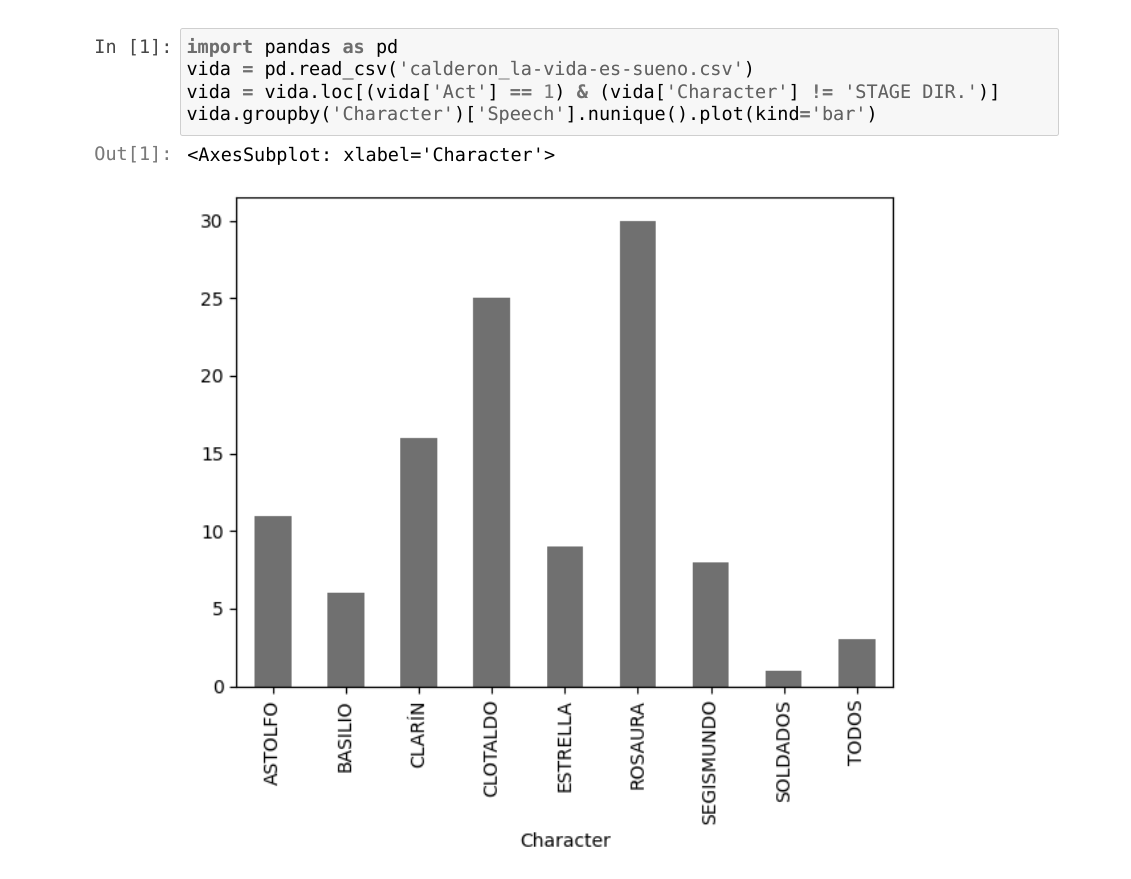
\includegraphics{images/pandasplot.png}}                             
	\caption{Ejemplo de aplicación.}
	\label{fig:pandasplot}
\end{figure}


La tabla permite un uso flexible y obtener información de manera rápida y sencilla. Por ejemplo, pueden compararse cuántas líneas dice cada personaje o, ya que disponemos del texto en sí, contar palabras por personaje (\Cref{fig:pandasplot}); podría asimismo diferenciarse entre personajes\index{personaje} femeninos o masculinos, o seguir el grado de participación de cada uno a lo largo de las escenas en función de sus parlamentos\index{parlamento}. Conociendo esto de cada una de las obras de un corpus, podrían compararse entre sí, en masa incluso, para encontrar piezas que se salgan de la norma. Si se agrupan, podría observarse las diferencias entre épocas, autores, géneros, o en función de varias variables, como la evolución de un autor en la producción de un género concreto a lo largo del tiempo.
\label{chap:7}
				\chapter{Transcripción automática}
\epigraphhead[50]{\epigraph{A las pronunciadas voces\\de blandas músicas junten\\sus no pronunciadas solfas\\las aves, siendo a su numen.}{Calderón, \textit{La nave del mercader}}}
\section{Sobre la transcripción automática}
\setcounter{exx}{0}
Para poder analizar digitalmente los diálogos acercándonos a su declamación, su representación grafémica convencional se antoja insuficiente. Al contrario que el lector de carne y hueso, el computador es incapaz de inferir la prosodia a partir del texto si no se le indica explícitamente. La máquina lee lo que se le ordene leer y lo interpreta como se le haya instruido hacerlo. Lo ideal sería olvidarnos de los textos y recurrir a grabaciones de calidad tomadas durante puestas en escena de las obras que deseemos examinar, tanto mejor si son recitadas por actores\index{actor} bregados en la interpretación de textos áureos. A partir de esas grabaciones podríamos extraer y estudiar la representación de las ondas sonoras. Sin embargo, la grabación proporcionaría la mejor descripción posible del sonido de \textit{cada} función, por lo que sus resultados solo serían totalmente válidos para sus respectivos casos \parencite[12]{sanchez2017}; otro elenco de actores, un nuevo director de escena o, incluso, las variaciones en la forma de entender el personaje tras representarlo un par de veces, conducirían a cambios en la entonación. Podríamos entonces tomar varias muestras diferentes, pero esto dispararía los recursos requeridos hasta hacer inasumible un estudio extenso.

Otro inconveniente que se plantearía a la hora de componer un corpus sería la necesidad impuesta por el material disponible, ya que este se limita a aquellas funciones de las que existe una grabación y esta es accesible. Como dijimos, la idea de la lectura distante\index{lectura distante} es, sin embargo, el examen del bosque y no de los árboles más altos. Y, si únicamente una mínima parte de piezas están editadas adecuadamente, un reducidísimo porcentaje de estas se lleva a las tablas. De esas representaciones, las que han sido grabadas son una minoría y, de esa minoría, solamente un porcentaje ínfimo se encuentra al alcance del público. Afortunadamente, hay un máximo común divisor entre interpretaciones, en el que todas las lecturas fieles concuerdan, por lo que no es necesario llegar a este de forma inductiva. Al contrario, el acuerdo de mínimos es el propio texto fijado. Nos adaptaremos, pues, a las condiciones a las que nos enfrentamos y nos conformaremos con el texto escrito, un modelo del objeto real. Como en todo modelo, hay elementos que se pierden, pero esto permite también concentrarse en los otros, los que hemos seleccionado. En nuestro caso, los fonológicos, a despecho de los sonidos auténticos de la representación.

En una función hay actores\index{actor} que median entre el texto escrito y lo que escucha el público. Esto es, los actores \textit{interpretan} el texto. Leen la grafía asumiendo que responde a unas reglas dadas y la pronuncian aplicando a lo que ven un conjunto de operaciones que han aprendido de antemano. Estas operaciones las desconoce el computador \textit{a priori}. Por suerte, el texto escrito según la ortografía normativa contiene casi toda la información necesaria para pronunciarlo, siempre y cuando se conozcan sus convenciones y las reglas que dictan como llevar a cabo la traducción. La ecuación $algoritmos + estructuras\: de\: datos = programas$ que da título a una obra clásica de la ciencia informática \parencite{wirth1976} sintetiza esta situación: la ortografía y la sintaxis española definen la forma en que se estructuran los datos de entrada, pero debemos definir los algoritmos que empleamos para tratarlos.

Estas operaciones se corresponden a las reglas de la fonología\index{fonología}, que el usuario competente de la lengua maneja orgánicamente y sin reparar en ello. Nuestra labor consiste en formalizarlas en una biblioteca informática que funcione de manera autónoma. Esto es, el programa principal importará un módulo de esta biblioteca en el que delegará la transcripción fonológica, de forma que, una vez introducida la cadena de texto a transcribir, recibe de vuelta su transcripción, aun sin ver lo que sucede entre bambalinas. Eso permitiría teóricamente sustituir este módulo por otro sin necesidad de modificar el programa principal, de modo que, ante la eventualidad de una solución mejor, sería trivial reemplazar la nuestra.

Al comenzar a trasladar los elementos teóricos a código, este módulo formaba parte integral de las funciones propias de la escansión. Sin embargo, poco tiempo después, se plantearon otros usos ajenos al originario, por lo que hubo que decidir entre reutilizar fragmentos del código en un programa nuevo independiente o externalizar los algoritmos de transcripción fonológica. Dado que la modularidad es una enorme ventaja a la hora de encontrar fallos, hacer modificaciones o añadir mejoras, optamos por lo segundo. Este desarrollo independiente también ha propiciado la introducción de nuevas funcionalidades que no se requieren en la investigación principal, pero que resultan de gran ayuda para otros fines, como la transcripción fonética y la transliteración a otras codificaciones. No obstante, además incluye funcionalidades orientadas exclusivamente a la lírica áurea, como la marcación de posibles haches aspiradas. La implementación en Python\index{Python} del módulo que detallamos en este capítulo está disponible de forma independiente como en la biblioteca \texttt{fonemas} \parencite{sanz2021sa} y \texttt{silabeador} \parencite{sanz2021sb}, cuyas versiones más recientes a fecha de publicación de estas páginas se encuentran en \Cref{list:fonemas}.

\section{Módulo transcriptor}
\subsection{Descripción general}
A grandes rasgos, el mecanismo consiste en tomar una cadena de caracteres y separarla en una lista, cada uno de cuyos elementos es una consonante, una vocal o una unión de vocales en caso de diptongo\index{diptongo} o triptongo\index{triptongo}. Después se recorre la lista para distribuir las consonantes en torno a los núcleos silábicos vocálicos. Finalmente, se establece la posición del acento prosódico de conformidad a las reglas ordinarias del español.

Gracias a este diseño modular, desde la perspectiva del procedimiento de escansión, la función transcriptora se reduce a un operador que recibe un verso y devuelve la transcripción de sus sílabas. Sin embargo, para llegar a ese resultado se requiere llevar a cabo una serie de procesos bajo la mesa para manipular el texto hasta dejarlo en su forma final. Simplificando los detalles del proceso, este consiste en aplicar reglas de transformación de primitivas a la cadena grafémica y, una vez transformada esta, invocar un módulo de división silábica para que separe las sílabas. En las siguientes líneas examinaremos cómo hemos construido el módulo de transcripción fonética (\Cref{list:importfon}), recorriendo paso a paso los procesos de transcripción y silabación. 

El programa requiere algunas funciones de bajo nivel para operar. Parte de ellas las provee el propio lenguaje de programación, mientras que otras específicas tenemos que definirlas nosotros primero para poder usarlas después. Por lo tanto, antes de todo, hemos de preparar el entorno para que disponga de cuanto vayamos a necesitar. De ahí que las primeras instrucciones carezcan de una finalidad operativa. Estas sirven para componer las estructuras de datos que requeriremos para llevar a cabo la transformación. Atendiendo a esto, importaremos funciones de los diversos módulos que vayamos a requerir: en la implementación real, serían procedimientos específicos; aquí, el buen entendimiento que aporta el lector al asumir pasos implícitos.

\begin{algorithm}[!ht] %or another one check
	\caption{Definiciones previas de la biblioteca.}\label{list:importfon}
	\Importar{$Bibliotecas$}\;
	\Fclase{\Valoresp{}}{
		\word \gets\ $\{\}$\;
		\slbs \gets\ $\{\}$\;
	}
\end{algorithm}


La \textit{clase}\footnote{En programación orientada a objetos\index{programación!orientada a objetos}, una \textit{clase} es una plantilla para crear instancias de una estructuras de datos (\textit{objetos}) a partir de unos valores iniciales. La clase describe variables (\textit{atributos}) y procedimientos (\textit{métodos}) para operar sobre estas.} de datos la requerimos para definir los valores que tomarán los \textit{atributos} del \textit{objeto} que representa el texto transcrito. Denominaremos a esta clase \Valoresp, y la dotaremos de dos atributos, válidos para los distintos tipos de transcripción que llevamos a cabo.  Cada uno de estos atributos contiene dos valores, que definimos como sendas listas vacías $palabras$ y $s\acute{\imath}labas$, cuyos elementos son palabras y sílabas transcritas, respectivamente.  Una vez disponemos de los módulos que requeriremos y definida la clase\index{clase} auxiliar que sirve de plantilla para los valores, tenemos lo necesario para empezar con la clase principal.

\subsection{Definición de la clase de transcripción}

Como se observa en el \Cref{list:transcriptionheader}, esta clase acepta un argumento \footnote{La implementación en Python admite además cuatro argumentos opcionales mpara alterar el comportamiento de la transcripción cuando las circunstancias así lo aconsejan, de forma que disponemos así de una herramienta flexible para usar en casos particulares.}. La clase \texttt{Transcripción} tiene asimismo cuatro atributos y cuatro métodos públicos que pueden emplearse sin restricciones en programas externos. El argumento obligatorio es el propio texto que deseamos transcribir. A este lo denominaremos $texto$ en la clase, y espera recibir una cadena de caracteres Unicode\index{Unicode}, sea en español o su transcripción en el \ac{afi}.

\begin{algorithm}[!ht] %or another one check
	\caption{Cabecera del módulo de transcripción.}\label{list:transcriptionheader}
	 \Fclase{\Transcripcion{$texto$}}{
	 	\texto \gets \Limpia{$texto$} \;
	 	\lIf{reordenar}{\texto \gets\  \Reordena{$texto$}}
	 	\fonologia \gets\ \FNL{$texto$} \;
	 	\fonetica \gets\ \FNT{$fonologia$} \;
	 	\sampa \gets\  \SAMPA{$fonetica$} \;
	 }
\end{algorithm}

Respecto a los atributos de la clase \texttt{Transcripción}, todos ellos deben ser accesibles desde el exterior. El primer atributo es $texto$, que almacena la cadena de caracteres resultante de preprocesar la entrada con los métodos descritos en \Cref{met:letters}. El atributo $fonolog\acute{\imath}a$ es el resultado de aplicar el método \texttt{TranscripciónFonológica}\index{fonología} al texto de entrada. Este contiene una instancia de la clase \Valoresp, que ya habíamos definido, y su contenido serán sendas listas de palabras y sílabas transcritas según el \ac{afi}. El atributo $fon\acute{e}tica$\index{fonética} se obtiene mediante la aplicación del método \texttt{TranscripciónFonética} al valor del atributo $fonolog\acute{\imath}a$. Como este, es una instancia de la clase \Valoresp, por lo que también contendrá subatributos $palabras$ y $s\acute{\imath}labas$, pero, en este caso, lo que almacena las transcripciones fonéticas del texto. Finalmente, el atributo $sampa$ es la salida del método \texttt{TransliteraciónSAMPA} cuando se le pasa el contenido de $fon\acute{e}tica$. Al igual que los dos atributos precedentes, contiene una instancia de \Valoresp con los subatributos $palabras$ y $s\acute{\imath}labas$, aunque con su transcripción al \acl{sampa} (SAMPA). 

\subsection{Excurso \Roman{excurso}: Argumentos de la implementación en Python}\stepcounter{excurso}
En la implementación en Python\index{Python}, incluimos los argumentos opcionales para indicar si las palabras monosilábicas han de marcarse con símbolo de sílaba tónica (/ˈ/ en \ac{afi}) o no. Esto es, \textit{eres tú} se resuelve por defecto como \textipa{/ˈeRes tu/}, aunque puede forzarse a \textipa{/ˈeRes ˈtu/} si así se lo indicamos. Lo hacemos mediante una variable de tipo booleano que está inicializada por defecto como $falso$. Si creamos una instancia de la clase de transcripción indicando que el valor de  ese argumento es $verdadero$, forzamos el comportamiento contrario al predefinido. En cualquier caso, aquí consideramos tan solo la sílaba acentuada de cada palabra hasta que, más adelante, el análisis morfosintáctico permita identificar los acentos prosódicos\index{acento!prosódico}. En la discusión que sigue lo obviaremos por ser irrelevante en el aspecto teórico.

El programa de Python ofrece la posibilidad de señalar explícitamente las haches a comienzo de palabra. Si bien la aspiración ya se había perdido en Castilla entrado el siglo \textsc{xvii} \parencite[91.3]{lapesa2008}, esta sobrevivía en hablas dialectales \parencite{salvador1982} —como lo eran las de muchos dramaturgos—, pero también en la poética como herramienta de compensación métrica. Por este motivo, conviene marcar la posición de las haches de manera que, en caso de varios hiatos posibles, la posible aspiración tenga valor determinante para inclinarse por esa sílaba. Se ha diseñado como una característica opcional para facilitar la transcripción de textos modernos, que no requieren de esta funcionalidad. De nuevo, ignoramos la capacidad de elegir de la que hemos dotado a la prueba práctica y marcaremos por defecto las haches iniciales para tenerlas en cuenta para valorar sinalefas. 

Otra opción es la capacidad de alterar la posición de los fonemas consonánticos en coda a final de palabra si la siguiente sílaba es vocálica, de manera que se evitan sílabas trabadas donde sea posible. De esta forma, si lo ponemos a $verdadero$, \textit{dos uno} se interpretará como /doˈsu.no/ en lugar de /dosˈu.no/. Esto responde a una cuestión fonética más que fonológica y no afecta a la calidad de los fonemas ni a su posición fonémica absoluta, sino únicamente a su posición relativa respecto a la serie silábica. En ciertas circunstancias puede resultar útil, pero no lo consideraremos aquí.

En el diseño para el uso en un escenario real, hemos tenido que introducir asimismo modificaciones más prácticas. Una de ellas es la opción de elegir el carácter que representa el acento primario en la transliteración \ac{sampa}. Esto responde a la necesidad de guardar en ocasiones los resultados en archivos en un archivo \ac{csv}, acrónimo de \textit{Comma Separated Values}. Este formato permite organizar información al modo tabular de una hoja de cálculo en texto plano, de manera que cada línea corresponde a una fila, cuyas columnas se separa una coma. En caso de que los valores de un campo lleven comas, estos se entrecomillan para indicar que todo cuanto se encuentre entre las comillas ha de interpretarse literalmente. \ac{sampa} emplea comillas dobles para señalar la posición de las sílabas tónicas, que, en un archivo \ac{csv}, se interpretan como una la apertura de una cadena de caracteres literal. Por esta razón, resulta necesario introducir un símbolo alternativo cuando se desea guardar información en un archivo de este tipo.

La implementación de Python también ofrece la posibilidad de decidir el comportamiento del programa ante una \textit{s} líquida. Esta función responde a la frecuencia con que se dan eses líquidas en los textos, sobre todo en fragmentos latinos intercalados, lo que hace necesario, por lo menos, tener en consideración su existencia. Estos casos se resuelven reinterpretando la consonante como coda de una vocal /e/ protética\index{epéntesis}.

\subsection{La \textit{s} líquida}
Aunque en la implementación de Python\index{Python} damos la posibilidad de desactivar la funcionalidad de solucionar esto observando la fonotáctica española, para la explicación daremos por sentada esta estrategia. La \textit{s} líquida es aquella en que /s/ aparece en ataque de la sílaba inicial seguida inmediatamente de consonante. Si bien era habitual en latín, desapareció en su evolución a algunas de las lenguas romances, el español entre ellas.  Los préstamos que la emplean, se resuelven mediante un /e/ protésica ante la \textit{s}. Este segmento gana carácter silábico, por lo que la sílaba inicial se desdobla \parencite[165]{claveria2018}.

¿De qué forma afecta este elemento al análisis de dramas del Siglo de Oro? Como decíamos, existen numerosas instancias de eses líquidas en los textos. Dado que los editores críticos de cada caso han optado por hacer una excepción en la modernización ortográfica y conservar la ortografía original, cabe pensar que esta decisión podría responder a un criterio fonológico.  Esto es, el verso \textit{spíritu ha de lograrla} del Ejemplo \ref{ex:spiritu4} se resolvería conforme a la edición como \textipa{/ˈspi.Ri.tu ˈa de lo.ˈgRaR.la/}, que, tras encontrar los acentos prosódicos, quedaría como $\{\acute{\imath},i,u,\acute{a},e,o,\acute{a},a\}$. Por el contrario, si introducimos una \textit{e} epentética,  la transcripción será \textipa{/esˈpi.Ri ˈtwa de lo.ˈgRaR.la/}, sus núcleos vocálicos se organizarían de la manera $\{e,\acute{\imath},i,\acute{a},e,o,\acute{a},a\}$ una vez hechas las sinalefas pertinentes. Estas dos soluciones producirían patrones rítmicos diferentes, \texttt{+--+--+-} y \texttt{-+-+--+-}.

La cuestión se torna más apremiante al considerar que, en muchas obras, se intercalan fragmentos latinos, a los que la ese líquida no es ajena, al contrario que sucede con su presencia en el español. ¿Debemos asumir que se conserva una ese líquida culta en las obras teatrales a imitación del modelo latino? Veamos los ejemplos que proporciona nuestro corpus de autos sacramentales, donde encontramos las siguientes instancias de ese líquida antecediendo a /p/ y /t/ o /k/:

\begin{exe}
	\ex\begin{xlist}
		\ex\label{ex:splendor}sin que una alba splendor de otra alba sea\\\strut\hfill(Calderón, \citetitle[17]{calderon_mariacorazon})		
		\ex\label{ex:spiritu}del Spíritu) toda\hfill(v. 179)	
		\ex\label{ex:splendor1}el spíritu encomiendo.\hfill(v. 1296)	
		\ex\label{ex:spiritus}los spíritus (¡qué ahogo!)\hfill(v. 1319)
		\ex\label{ex:stella}Ave, maris stella\hfill(v. 1481)	
		\ex\label{ex:spiritui}Spiritui Santo\hfill(v. 1517)
	\end{xlist}
	\ex\begin{xlist}
		\ex\label{ex:spiritu1}Spíritu de Dios era\strut\hfill(\citetitle[246]{calderon_pernaso})	
		\ex\label{ex:spiritual}el dulce spiritual\hfill(v. 551)	
		\ex\label{ex:spiritual1}del spiritual manjar\hfill(v. 883)	
		\ex\label{ex:spiritu2}Spíritu de consuelo.\hfill(v. 1207)
		\ex\label{ex:speravi2}In te, Domine, speravi,\hfill(v. 1237)
		\ex\label{ex:scitura}carear estos dos testos de Scritura,\hfill(v. 1510)
		\ex\label{ex:spiritu3}Yo un nuevo spíritu en este\hfill(v. 1984)
	\end{xlist}
	\ex\label{ex:speravi}In te, Domine, speravi,\strut\hfill(\citetitle[2200,2202]{calderon_fernando2})
	\ex\label{ex:splendor2}su splendor se presume\strut\hfill(\citetitle[302]{calderon_curaenfermedad})
	\ex\label{ex:scena}a la imaginada scena\strut\hfill(\citetitle[354]{calderon_redencioncautivos})
	\ex\label{ex:spiritu4}spíritu ha de lograrla,\strut\hfill(\citetitle[1738]{calderon_espigasruth})
	\ex\label{ex:splendor3}te da el splendor divino\strut\hfill(\citetitle[796]{calderon_alimentoshombre})
\end{exe}
Aunque la mayoría de los casos mostrados arriba permiten una resolución aceptable mediante poco más que jugar con las sinalefas y las diéresis\index{diéresis}, en (\ref{ex:spiritu}) necesitamos la epéntesis para alcanzar el heptasílabo, que es como los versos colindantes aconsejan escandirlo. Por ese motivo, resulta apropiado disponer de la opción de intercalar una vocal antes de la ese líquida.

Más dificultad plantea el caso de (\ref{ex:spiritual}). Aquí debemos contar ocho sílabas, por lo que, si hacemos la epéntesis, se plantea la dicotomía de no hacer sinalefa\index{sinalefa} en \textit{dulce espiritual}, forzando un hiato\index{hiato} entre dos vocales iguales, ambas átonas, o recurrir a la diéresis\index{diéresis} en \textit{espiritual}, lo que además sería su pronunciación regular. Esta última posibilidad se antoja más plausible, por lo que el verso no ofrece pistas sobre la epéntesis, pues no influiría en la resolución. En (\ref{ex:spiritual1}) encontramos el caso contrario: si hacemos epéntesis, debemos diptongar \textit{espiritual} para que el verso siga siendo octosílabo. El ritmo aporta poca ayuda, ya que ambas soluciones serían \texttt{----+--}. La solución no epentética ˈ\textipa{/del spi/} implicaría el préstamo fonológico latino. La otra ordenación posible, \textipa{/dels pi/} también es ajena a la fonología española, donde /ls/ en coda se da exclusivamente en préstamos y nunca en interior de palabra.

En cuanto a la pronunciación latina, tenemos (\ref{ex:stella}), (\ref{ex:spiritui}) y (\ref{ex:speravi}). En los dos primeros casos nos hallamos ante hexasílabos cantados y ante un octosílabo en el último. El octosílabo aporta poco a la discusión, pues la sinalefa provocaría que el verso se resolviera exactamente igual con o sin epéntesis, por lo que discutiremos los otros dos. El ejemplo (\ref{ex:stella}) es un verso cantado por los músicos, y debe leerse en consonancia con la pronunciación latina para concordar con el verso posterior \ref{ex:stellapos}, así como con los siguientes parlamento de los músicos (\ref{ex:celli} y \ref{ex:stellapospos}).

\begin{exe}\ex\begin{xlist}
		\ex Dei mater alma\strut\hfill(Calderón, \citetitle[1482]{calderon_mariacorazon})\label{ex:stellapos}
		
		\ex\label{ex:celli}Atque semper virgo,\\felix celli porta.\hfill(vv. 1485-1486)
		
		\ex Summens illud Ave\\Gabrielis ore.\hfill(vv. 1489-1490)\label{ex:stellapospos}
	\end{xlist}
\end{exe}
El verso \ref{ex:spiritui} es ambiguo, por prestarse a la resolución tanto mediante epéntesis como diéresis\index{diéresis}. En este último caso, no obstante, obligaría a acentuar la vocal cerrada, provocando un acento antirrítmico. Parece más probable que de nuevo se alcance el metro valiéndose de la epéntesis. De esta manera, la estrategia protésica se antoja la solución más cabal a este tipo de palabras, trátense de voces españolas o no.

No hay que descartar, sin embargo, que puedan darse casos en los que se prefiere la pronunciación latina. Véase por ejemplo el siguiente ejemplo en \ref{ex:caribdis}, que, aun sin proceder de una obra teatral, obliga a tomar precauciones:

\begin{exe}\ex\label{ex:caribdis}En Scilas ni en Caribdis no repara\\\strut\hfill(Cervantes, \citetitle[Lib. 1, cap. 9]{cervantes2004})
\end{exe}

En situaciones como esta, posponemos la resolución hasta el ajuste métrico, dejando abierta la posibilidad de eliminar la epéntesis y emplear la pronunciación latina si lo demanda el verso para obtener el recuento silábico apropiado. No obstante, en el caso del teatro, en el que la declamación se aproxima más al habla corriente que en la lírica —sea siquiera porque  la mayor cantidad de versos dificultan esmerarse tanto en cada uno como se haría, por ejemplo, con los catorce versos de un soneto—, cabría plantearse hasta qué punto el actor\index{actor} tendería a resolver un verso semejante forzando la pronunciación latina en lugar de añadir una sílaba supernumeraria atendiendo a la fonología española.

\subsection{Preprocesado}\label{met:letters}
El preprocesado tiene como meta eliminar, enmendar y expandir caracteres. Por una parte, elimina del texto todos aquellos caracteres no alfabéticos que se encuentren en él. Por otro lado, deletrea los nombres de las consonantes en caso de encontrar una como un grafema aislado, de manera que transcriba \textit{letra b} no como \textipa{/ˈletRab/} sino como \textipa{/ˈletRa ˈbe/}. Finalmente, translitera diacríticos ajenos al repertorio del español. Para llevar a cabo la tarea definimos la función que describimos en \Cref{list:preprocesado}. Esta recibe como entrada el texto que deseamos preparar y lo devuelve preprocesado.

En primer lugar, definimos las equivalencias entre los grafemas consonánticos y su deletreo, lo que en \Cref{list:preprocesado} hemos llamado $letras$. La finalidad de esto es instruir al computador para tratar consonantes aisladas que encuentre en el texto, como en \ref{ex:abc}, pues la máquina ignora la pronunciación; si no le indicamos que haga una excepción, tomará la consonante aislada como un grafema y no como el nombre de una letra, por lo que la sustituirá por el fonema correspondiente. Salvo en el caso de las vocales, esto produciría palabras monofonemáticas consonánticas, ajenas por completo a la fonología española\index{consonante}. Dicho de otro modo, si encuentra \textlangle{}b\textrangle{} sin contexto ha de tratarlo como \textlangle{}be\textrangle{} y si da con \textlangle{}h\textrangle{}, como \textlangle{}hache\textrangle{}. Para evitarlo, deletreamos el nombre de cada letra no vocálica cuando aparece una consonante aislada y hacemos una sustitución si es menester.

\begin{exe}
	\ex	\label{ex:abc}
	El abecé del marido.\\
	La A, quiere decir hacer\\
	La B significa bobo\\
	La C, callar; atended:\\
	«hacerte bobo y callar» ,\\
	¿qué os parece el abecé?\\\strut\hfill(Mira de Amescua, \citetitle[177-182]{mira_pastoresbelen})
\end{exe}

Excluiremos no obstante \textlangle{}y\textrangle{}, dado que en su valor de conjunción tiene pronunciación vocálica monofonemática. En el corpus no hemos encontrado ningún ejemplo de su uso literal como letra, valga la redundancia, mientras que su uso conjuntivo es extensivo, por lo que optamos por considerar únicamente la transcripción vocálica del grafema. Si ocurriera un caso que requiriese la transcripción \textipa{/ˈiˌgRje.ga/}, la transcripción /i/ que empleamos obligaría a resolver el verso con entre una y dos sílabas de menos respecto a las reales, dependiendo de la distribución de las sinalefas\index{sinalefa}, por lo que se evidenciaría la irregularidad del metro, lo que facilitaría sobremanera su localización y corrección manual.

\begin{algorithm}[!ht] %PREPROCESADO
	\caption{Módulo de preprocesado.}\label{list:preprocesado}
	\Fclase{\Limpia{texto}}{
		\letras \gets\ $\{a, b, c, d, ...\}$\;
		\deletreo \gets\  $f: \{(grafema_{1}, deletreo_{1}), ..., (grafema_{n}, deletreo_{n})\}$\;
		\simbolos \gets\  $f: \{s\acute{\imath}mbolo_{1}, ..., s\acute{\imath}mbolo_{n}\}$\;
		\diacriticos \gets\  $f: \{(diacr\acute{\imath}tico_{1}, transliteraci\acute{o}n_{1}), ..., (diacr._{n}, transl._{n})\}$ \;
		\texto \gets\  \Minuscula{$texto$} \;
		\ForEach{$car\acute{\imath}cter\:\in\:deletreos$}{
			\If{$letras_{i} \:\nsucc\:car\acute{a}cter\:\nsucc\ letras_{j}$}{
				\caracter \gets\  $deletreos_{car\acute{a}cter}$ \;
			}
		}
		\Return{texto}
	}
\end{algorithm}

Algunos caracteres pueden transcribirse de forma directa a su equivalente fonológico. En concreto, esto es posible si grafema\index{grafema} y fonema son homógrafos o si el fonema no tiene equivalente grafémico. Por eso transcribiremos directamente algunos grafemas a su fonema, mientras que otros han de conservar momentáneamente la representación grafémica para no alterar transformaciones posteriores. De esta manera, escribimos \textlangle{}haʧe\textrangle{}, pues el grafema \textlangle{}a\textrangle{} existe como fonema y se corresponde biunívocamente con este. Por el contrario, el grafema \textlangle{}r\textrangle{} puede representar \textipa{/R/} o \textipa{/r/} si está duplicado. Esto desaconseja alterarlo previamente. El grafema \textlangle{}ch\textrangle{} tiene también correspondencia biunívoca con el fonema /ʧ/. Al no existir el grafema \textlangle{}ʧ\textrangle{} en el repertorio del español, no hay reglas posteriores que le afecten y lo transcribiremos \textlangle{}haʧe\textrangle{}, sin que afecte a operaciones ulteriores. La \textit{h} inicial, no obstante, hemos de conservarla para decidir más adelante si la marcamos como posible aspiración.

A continuación, creamos una lista de signos ortográficos de puntuación\index{puntuación} que llamaremos $s\acute{\imath}mbolos$. Al carecer de equivalente fonemático, no se necesita definir una transformación para cada uno, pues todos ellos serán reemplazados por un elemento vacío. En previsión de diferentes estilos ortotipográficos —tanto aceptados como no—, debemos incluir todas las variaciones posibles. Por ejemplo, comillas españolas e inglesas, tanto rectas como rizadas, simples y dobles. También, grafías irregulares de la raya ortográfica  (—) y el guion  (-). Hemos comprobado que la fidelidad a las prescripciones académicas \parencite[373]{rae2010} varía notablemente de un texto a otro, por lo que, además de los susodichos símbolos, hemos incluido la raya intermedia\footnote{Aunque no es propia del español, se usa extensivamente en inglés (\textit{en dash}) y en alemán (\textit{Halbgeviertstrich}), por lo que no es extraño encontrar ocasionalmente este símbolo reemplazando la raya española en ediciones poco cuidadas.} {(–)}.

Seguidamente, tratamos grafemas\index{grafema} ajenos a la ortografía española o aquellos que, formando parte del repertorio castellano, se hallan modificados por un símbolo diacrítico extraño a este. Para ello definimos de nuevo las equivalencias entre los caracteres con diacrítico foráneo y su transliteración según las normas de la ortografía  española. No es raro hallar ediciones que emplean diacríticos\index{diacrítico} y ligaturas\index{ligatura} de diversas lenguas, como el alemán (\ref{ex:de}), el catalán (\ref{ex:cat}), el italiano en Lope (\ref{ex:it}) o el latín (\ref{ex:lat}).
\begin{exe}
	\ex\begin{xlist}
		\ex\label{ex:de}El húngaro a Nördlingen\\\strut\hfill(Calderón, \citetitle[113]{calderon_blason})		
		\ex\label{ex:cat}¿Què voleu? Les paradetas\strut\hfill(\citetitle[1868]{calderon_pintordeshonra})
		\ex\label{ex:lat}mutans Evæ nomen\strut\hfill(\citetitle[1494]{calderon_mariacorazon})
		\ex\label{ex:pt}porque el gran Luis de Camões\\\strut\hfill(\citetitle[106]{calderon_secretoagravio})
		\ex\label{ex:it}Un seculo e più, segnora,\strut\hfill(Lope de Vega, \citetitle[3054]{vega_anzuelofenisa})
	\end{xlist}
\end{exe}

Estos símbolos diacríticos\index{diacrítico} poco comunes pueden darse incluso en palabras patrimoniales españolas, sea por una ortografía arcaizante o por una cuestión editorial. De esta manera, dependiendo de la edición, se encuentran acentos circunflejos en sustitución de un dígrafo vocálico con reducción fonética (\ref{ex:espant1}), el anticuado acento grave (\ref{ex:espant2}) o la no menos antigua cedilla (\ref{ex:espant4}), al lado de la habitual diéresis\index{diéresis} editorial mediante crema para señalar un hiato\index{hiato} (\ref{ex:espant3}).
\begin{exe}
	\ex\begin{xlist}
		\ex\label{ex:espant1}hoy vengo buscándôs: basta\strut\hfill(Calderón, \citetitle[61]{calderon_amarmuerte})\\
		decirle que crêr en Dios.\strut\hfill(v. 549)
		\ex\label{ex:espant2}Conmigo à un tiempo y con ella,\strut\hfill(\citetitle[1868]{calderon_pintordeshonra})
		\ex\label{ex:espant4}A ti te pareçe eso,\strut\hfill(\citetitle[1005]{calderon_diablomudo})	\ex\label{ex:espant3}te parece que Dïana,\strut\hfill(\citetitle[484]{calderon_verdaderodiospan})
	\end{xlist}
\end{exe}
La solución pasa por la transliteración\index{transliteración}, cuyo caso general consiste simplemente en eliminar el diacrítico. No obstante, debemos considerar algunas excepciones. El acento grave suele indicar una sílaba tónica tanto en otras lenguas como en grafías anticuadas del español, salvo en el caso de palabras monografémicas. Así pues, primero los grafemas \textlangle{}à\textrangle{} y \textlangle{}ò\textrangle{} por  \textlangle{}a\textrangle{} y \textlangle{}o\textrangle{} cuando van orlados por espacios en blanco, y todos los demás casos por su equivalente con acento agudo.

Las ligaturas\index{ligatura} pueden o bien desdoblarse en dos grafemas, por lo que representarían dos sílabas ortográficas, o bien transliterarlas al grafema del repertorio español que represente el sonido más cercano. Tradicionalmente, \textlangle{}æ\textrangle{} ha dado el diptongo /je/ o /e/ (considérese \textit{cielo} y \textit{celestial}, ambas voces procedentes del latín \textit{cælus}), como vimos en el ejemplo \ref{ex:celli}.

En caso de encontrar diéresis\index{diéresis}, diferenciaremos entre las editoriales y las ortográficas. Para las primeras, sustituimos por el grafema sin símbolo diacrítico y añadimos un guion bajo precediendo a la vocal para señalar más tarde al módulo de división silábica que ahí ha de romper el diptongo. Finalmente, reemplazamos el grafema \textlangle{}ç\textrangle{} por \textipa{/T/}, pues su pronunciación anterior \textipa{/\texttoptiebar{ts}/} debía de haber completado la desafricación ya en la segunda mitad del siglo \textsc{xvi} \parencite[92.4]{lapesa2008}. En caso de que la diéresis proceda de un extranjerismo, se trata indistintamente, asumiendo que se translitera como una de las cinco vocales españolas y no como un diptongo o un fonema ajeno a la fonología española.

Ahora ya disponemos de las descripciones de los elementos que emplearemos para hacer las sustituciones. Por una cuestión de eficiencia, convertimos el texto a minúsculas antes de empezar a sustituir. De otra manera, estaríamos obligados a evaluar cada vez si estamos ante una variación mayúscula o minúscula de una misma letra. Esto duplicaría el tiempo de la operación, lo que podría resultar perceptible cuando se procesa una gran cantidad de texto, como es frecuente en nuestro caso. Con el texto en minúscula, cada letra está representada por un único grafema y no se da este problema.

La primera de las series de sustituciones consiste en recorrer las claves de $letras$ y, si encuentra una ocurrencia de una de ellas que no esté orlada a izquierda y derecha por otras letras, estamos ante una consonante aislada, por lo que procedemos a sustituir las ocurrencias de esa letra solitaria en el texto por el valor de la clave correspondiente.
\[x \longrightarrow f(x)\;/\; \emptyset \_\ \emptyset\]

A continuación recorremos la lista de símbolos y sustituimos las ocurrencias  de sus elementos en el texto por un espacio en blanco. De esta manera tenemos únicamente palabras.
\[x \longrightarrow \emptyset\]


Para finalizar introduciremos los casos de \textit{e} epentética. Sustituimos \textlangle{}s\textrangle{} en posición inicial de palabra siempre que no vaya seguido por una vocal.
\[\text{s} \longrightarrow \text{e}, \text{s}\;/\; \emptyset \_ {\scriptstyle\langle{}-VOC\rangle{}}\]
Tras realizar estas operaciones, el método devuelve la cadena de caracteres transformada.

\subsection{Excurso \Roman{excurso}: Reordenación}\stepcounter{excurso}
El segundo de los métodos de preprocesado lo contemplamos como idea para la traducción computacional de los algoritmos vistos aquí. Se emplea si el argumento para reordenar del programa de Python se ha puesto deliberadamente a $verdadero$. Para la escansión no lo utilizaremos, salvo que necesitemos afinar con una agrupación silábica fonológica, ya que los núcleos vocálicos permanecen constantes. El objeto es, pues, proporcionar unas herramientas tan flexibles como podamos producir y, para ello, como en este caso, intentamos adelantarnos a las necesidades de los hipotéticos beneficiarios de la biblioteca.

\begin{algorithm}[!ht] %or another one check
	\caption{Módulo de reordenación.}\label{list:reordena}
	\Ffuncion{\Reordena{texto}}{
		\vocales \gets $\langle vocales\rangle$\;
		\ForEach{$posici\acute{o}n_{i} \in\:texto$}{
			\cuenta \gets $\lvert posici\acute{o}n_{i}\rvert$ \;
			\If{$i \neq 0\:\wedge \lvert posici\acute{o}n_{n-1}\rvert > 1$}{
				\If{$posici\acute{o}n_{i}\:\text{\empiezacon}\:vocales$}{
					\If{$posici\acute{o}n_{i-1}\:\text{\neg \acabacon}\:vocales$}{
						$\posicion_{i}$ \gets\ $posici\acute{o}n_{i-1, n} + posici\acute{o}n_{i}$ \;
						$\posicion_{i-1}$ \gets\ $posici\acute{o}n_{i-1} -\:posici\acute{o}n_{i-1, n}$ \;
					}
				}
			}
		}
		\Return{texto}
	}
\end{algorithm}

En \Cref{list:reordena} vemos cómo se lleva a cabo. Tomamos el texto y empezamos a recorrerlo por sus sílabas. Queremos comprobar si la sílaba correspondiente a cada iteración no es la primera del texto, esto es, si existe una sílaba precedente plurifonemática cuya coda es redistribuible. De cumplirse todas las condiciones, nos aseguramos de que la sílaba que estamos examinando empiece por vocal y la anterior acabe por consonante, en cuyo caso procederemos a reubicar la última consonante de la coda de la sílaba precedente en el ataque de la sílaba actual. 

\subsection{Transcripción fonológica}\label{met:fnl}
Con el texto de entrada dispuesto, se aborda la transcripción fonológica\index{fonología}. Esta se produce mediante las tablas y reglas de sustitución del método \texttt{TranscripciónFonológica}, cuyas primeras líneas vemos en el \Cref{list:transcriptionfnl}. Toma como argumento una variable $texto$, además de heredar una instancia de la clase \texttt{TranscripciónFonológica}. El argumento $texto$ es una copia del texto a transcribir. 

\begin{algorithm}[!ht] %FNL
	\caption{Método de transcripción fonológica.}\label{list:transcriptionfnl}
	\Fmetodo{\FNL{texto}}{
		\diacriticos \gets\  $f: \{diacr\acute{\imath}tico_{1}: transliteraci\acute{o}n_{1}), ..., diac._{n}: transl._{n}\}$\;
		\consonantes \gets\  $f: \{grafema_{1}: fonema_{1}, ..., grafema_{n}: fonema_{n}\}$\;
		\texto \gets\ \erre{texto}\;
		\If{aspiración}{
			\texto{$\langle h\rangle$} \gets  $marca, \forall \emptyset \succ h \in texto$\;
		}
		\texto{$consonantes_{c}$} \gets $consonantes_{v}, \forall consonantes_{c} \in texto$\;
	}
\end{algorithm}

Antes de empezar a modificar el texto, definimos una tabla de sustitución de grafemas con diacrítico y su equivalente sin este. Para ello, nos valemos de un \textit{diccionario}, como especificamos el tipo de datos consistente en un conjunto de pares \textit{clave}\index{diccionario!clave}, \textit{valor}\index{diccionario!valor}. La clave nombra al elemento y el valor, como su propio nombre indica, es el contenido que asignamos al elemento nombrado por la clave. De esta manera, creamos claves con todos los grafemas vocálicos con símbolo diacrítico y les damos como valor su equivalente sin diacrítico. Por ejemplo, $\{\acute{a}: a, \grave{a}: a, ..., \ddot{u}: u\}$. Se incluye de manera adicional la raya baja, pues la emplearemos para señalar hiatos\index{hiato} en caso de diéresis\index{diéresis}. Al no ser esta más que una marca diacrítica, no le corresponde fonema alguno.

Definimos un segundo diccionario para los sonidos consonánticos. Este también tiene un grafema o una combinación grafémica como claves, pero sus valores son sus respectivos fonemas equivalentes en la forma $\{v: b, z: \theta, qu: k, ...\}$. Al contrario que el diccionario anterior, este contiene combinaciones fonológicas para tener en cuenta el contexto, de modo que crearemos dos claves distintas $ce$ y $ca$, a las que asignaremos además valores diferentes $\theta e$ y $ka$. Las claves deben seguir un orden específico que refleje cómo deben ser aplicadas las transformaciones. Por ejemplo, en el caso de \textlangle{}j\textrangle{},  $x$ debe preceder a $j$ en el diccionario. De lo contrario (\ref{ex:xj}), estaríamos ante una transformación errónea, pues si transforma primero $j$, al llegar a la siguiente, se encontraría con caracteres $x$ que corresponderían tanto al grafema \textlangle{}x\textrangle{} como al fonema /x/.

\begin{exe}
	\ex\label{ex:xj}\strut\hfill\begin{tabular}{ l|*{3}{c}} 
		entrada: &  \multicolumn{1}{|c|}{a} &  \multicolumn{1}{|c|}{j} &  \multicolumn{1}{|c|}{o} \\ 
		$\text{j} \longrightarrow \text{x}$ &   &  \uparrow& \\
		&   \multicolumn{1}{|c|}{a} &  \multicolumn{1}{|c|}{x} &  \multicolumn{1}{|c|}{o}\\
		$\text{x} \longrightarrow \text{ks}$ &   &   \uparrow &  \\
		salida: &   \multicolumn{1}{|c|}{a} &  \multicolumn{1}{|c|}{ks} &  \multicolumn{1}{|c|}{o} \\
	\end{tabular}\hfill\strut
\end{exe}

Las sustituciones comienzan por el grafema \textlangle{}r\textrangle{}\index{consonante!vibrante} cuando le corresponde el fonema /r/. Dado que el mismo símbolo se emplea para el grafema correspondiente a \textipa{/R/}, sustituimos los grafemas de /r/ por el carácter \texttt{R}, esto es, detrás de \textlangle{}n\textrangle{}, \textlangle{}n\textrangle{} o \textlangle{}s\textrangle{} o a comienzo de palabra, o si \textlangle{}r\textrangle{} aparece duplicado.

\[\text{r} \longrightarrow \text{R}\;/\; \Bigg\{\begin{smallmatrix} \text{\normalsize{n}} \\ \text{\normalsize{l}} \\ \text{\normalsize{s}} \\ \emptyset\end{smallmatrix}\Bigg\} \_\]
\[\text{r}, \text{r} \longrightarrow \text{R} \]

A continuación comprobamos si existen instancias de del grafema \textlangle{}h\textrangle{} a comienzo de palabra. De ser así, las sustituimos por una marca en lugar de hacerlas desaparecer como las interiores. Esto tiene por objetivo advertir de la presencia de esta hache, de manera que pueda tenerse en cuenta después a la hora de predecir una potencial aspiración. Seguidamente, recorremos las claves del diccionario $consonantes$ y, cuando alguna de ellas aparece en el texto, sustituimos todas sus instancias por el valor de la clave correspondiente. Esto, sin embargo, no es suficiente para tratar las transformaciones en su totalidad porque \textlangle{}y\textrangle{} y \textlangle{}g\textrangle{} presentan particularidades de tal cariz que hacen necesario un tratamiento específico (\Cref{list:fonemay}).

\begin{algorithm}[!ht] %Y
	\caption{Caso de \textlangle{}y\textrangle{}.}\label{list:fonemay}
	\texto{\textlangle\text{y}\textrangle} \gets  $/i/, \forall \emptyset\nsucc\langle y\rangle\nsucc\emptyset \in texto$\;
	\texto{$\langle y\rangle$} \gets $/j/, \forall \langle y\rangle\nsucc\emptyset \in texto$\;
	\texto{$\langle y\rangle$} \gets $/\textsl{ʝ}/, \forall \langle y\rangle \in texto$\;
	\texto{$diacr\acute{\imath}ticos_{v} + /\textsl{ʝ}/$} \gets  $diacr\acute{\imath}ticos_{c}/i/,$\\ \Indp
	$\forall diacr\acute{\imath}ticos_{v} + /\textsl{ʝ}/\nsucc\emptyset, diacr\acute{\imath}ticos_{v} \in \{\langle\acute{a}\rangle, \langle\acute{e}\rangle, \langle\acute{\imath}\rangle, \langle\acute{o}\rangle, \langle\acute{u}\rangle\}$\;\Indm
	\consonantes \gets\ $f: consonantes$\;
	\texto{$/\textsl{ʝ}/$} \gets $/i/, \forall /\textsl{ʝ}/ + consonantes_{n} \in texto$\;
\end{algorithm}

En el caso de que detectemos que el texto contiene el grafema \textlangle{}y\textrangle{}, se sustituyen todas las ocurrencias aisladas de esta, correspondientes a la conjunción, por /i/. Si aparece a final de palabra, se considera como semiconsonante parte de un diptongo decreciente, por lo que se reemplaza por /j/. En los demás casos, se cambia a /ʝ/.

\[\text{y} \longrightarrow \text{i}\;/\;\emptyset \_ \emptyset\]
\[\text{y} \longrightarrow \text{j}\;/\; \_ \emptyset\]
\[\text{y} \longrightarrow \text{ʝ}\]

El paso siguiente consiste en tomar las claves con acento agudo del diccionario $diacr\acute{\imath}ticos$ para sustituir su valor  —esto es, la vocal sin acento— en el texto por la vocal acentuada si la vocal precede a a /ʝ/ a final de palabra.

\[\Bigg\{\begin{smallmatrix}\text{\normalsize{a}}\\\text{\normalsize{e}}\\\text{\normalsize{i}}\\\text{\normalsize{o}}\\\text{\normalsize{u}}\end{smallmatrix}\Bigg\}, \text{ʝ} \longrightarrow \Bigg\{\begin{smallmatrix}\text{\normalsize{á}}\\\text{\normalsize{é}}\\\text{\normalsize{í}}\\\text{\normalsize{ó}}\\\text{\normalsize{ú}}\end{smallmatrix}\Bigg\}, \text{i} \;/\;  \_ \emptyset\]

Para finalizar el tratamiento excepcional de \textlangle{}y\textrangle{}, se comprueba que no se ha introducido accidentalmente /ʝ/ seguido de consonante y, de ser así, se reemplaza por \textlangle{}i\textrangle{}.

\[\text{ʝ} \longrightarrow \text{i} \;/\; ⎄\_ {\scriptstyle\langle{}+CONS\rangle{}}\]

El segundo grafema que tratamos de manera excepcional es \textlangle{}g\textrangle{}\index{consonante!velar}, ya que este puede representar los fonemas /g/ y /x/ dependiendo del contexto. Para ello, confirmamos en primer lugar si este aparece en $texto$ para, de darse tal circunstancia, emprender los pasos oportunos para su tratamiento (\Cref{list:fonemag}).

\begin{algorithm}[!ht] %Y
	\caption{Caso de \textlangle{}g\textrangle{}.}\label{list:fonemag}
	\debiles \gets $\:f: \{e, i\}$ \;
	\fuertes \gets $\:f: \{a, o, u\}$ \;
	\If{$\langle g\rangle\in texto$}{
		\texto{$\langle g\rangle + d$} \gets $\langle x\rangle + d, \forall \langle g\rangle + d \in texto, \forall d \in d\acute{e}biles$ \;
		\texto{$\langle gu\rangle + d$} \gets $\langle g\rangle + d, \forall \langle g\rangle + d \in texto, \forall d \in d\acute{e}biles$ \;		
		\texto{$\langle g\ddot{u}\rangle + d$} \gets $\langle gw\rangle + d, \forall \langle g\ddot{u}\rangle + d \in texto, \forall d \in d\acute{e}biles$ \;
		\texto{$\langle gu\rangle + f$} \gets $\langle gw\rangle + f, \forall \langle gu\rangle + f \in texto, \forall f \in fuertes$ \;
	}
\end{algorithm}

En este caso, se procede primero a asignar el fonema /x/ a los grupos \textlangle{}ge\textrangle{} y \textlangle{}gi\textrangle{} y /g/ a \textlangle{}gue\textrangle{} y \textlangle{}gui\textrangle{}. Consideramos más allá de las formas canónicas de \textlangle{}e\textrangle{} e \textlangle{}i\textrangle{} e incluiremos sus variaciones diacríticas.
\[
\text{g} \longrightarrow \text{x} \;/\; \_
\Big\{
\begin{smallmatrix}\text{\normalsize{e}}\\\text{\normalsize{i}}\end{smallmatrix}\Big\}\]
\[
\text{g},\text{u} \longrightarrow \text{g} \;/\; \_ 
\Big\{
\begin{smallmatrix}\text{\normalsize{e}}\\\text{\normalsize{i}}\end{smallmatrix}\Big\}
\]
Para completar \textlangle{}g\textrangle{}, abordamos los casos en los que va seguido de  \textlangle{}u\textrangle{} con o sin diéresis. 
\[
\text{g}, \text{ü}\longrightarrow \text{g}, \text{w} \;/\; \_
\Big\{
\begin{smallmatrix}\text{\normalsize{e}}\\\text{\normalsize{i}}\end{smallmatrix}\Big\}\]
\[
\text{g},\text{u} \longrightarrow \text{g}, \text{w} \;/\; \_ 
\Big\{
\begin{smallmatrix}\text{\normalsize{a}}\\\text{\normalsize{o}}\end{smallmatrix}\Big\}
\]

Con esto habríamos terminado prácticamente de transcribir los caracteres grafémicos en fonológicos. No obstante, quedan algunos diacríticos vocálicos que necesitamos para dividir el texto en palabras, que es precisamente de lo que se ocupan las líneas finales del método (\Cref{list:fnlreturn}). Esta división pasa por invocar al método \texttt{DivideVariables} (\Cref{list:dividevariables}), pasándole como argumentos $texto$. Este crea una instancia de la clase \Valoresp, que asignamos a la variable $transcripci\acute{o}n$ —enseguida entraremos en detalle en su modo de operar—. Para finalizar, como ya no son necesarios los símbolos diacríticos una vez termina la división silábica, los sustituimos por las formas canónicas en $transcripci\acute{o}n$ antes de devolver este objeto como salida.

\begin{algorithm}[!ht] %Y
	\caption{Caso de \textlangle{}y\textrangle{}.}\label{list:fnlreturn}
	\transcripcion \gets \DivideVariables{$texto$} \;
	\transcripcion{$diacr\acute{\imath}ticos_{c}$} \gets $diacríticos_{v}$ \;
	\Return{transcripción}
\end{algorithm}


\section{Métodos auxiliares de la transcripción}
\subsection{División entre palabras y sílabas}
Como hemos dicho, para transcribir fonológicamente empleamos el método \texttt{DivideVariables}. Este, a su vez, delega algunas de sus tareas en otros. Veamos primero el mecanismo general del método y, cuando lo tengamos, entremos en sus componentes, de una manera parecida a lo que acabamos de hacer con \texttt{TranscripciónFonológica}. Primero de todo, definimos las variables $palabras$ y  $s\acute{\imath}labas_{texto}$, que son las listas donde iremos almacenando todas las palabras y las sílabas del texto —debemos diferenciarla de la variable $s\acute{\imath}labas_{palabra}$, en la que almacenaremos las sílabas de una palabra cada vez—. Hecho esto, empezamos a iterar por los componentes que resultan de dividir el texto en una lista con las palabras de las que se compone.

Comprobamos si la palabra que estamos evaluando es un adverbio en \textit{-mente}\index{adverbio!{en -mente}@{en -\textit{mente}}}. Para ello, verificamos en primer lugar que esa sea efectivamente su terminación y que tenga más de cinco letras. Si este es el caso, guardamos en las variables $s\acute{\imath}labas$ y $t\acute{o}nica$ los resultados del método \texttt{Silabación} si le pasamos la raíz de la palabra, —esto es, excluyendo \textit{-mente}—. Trataremos \texttt{Silabación} por ahora como una caja negra, en la que introducimos la palabra por un extremo y sacamos del otro sus sílabas, sin preocuparnos de lo que sucede internamente para que esto ocurra; dejaremos para más adelante la descripción analítica de su mecanismo (\Cref{sec:silabeador}). Retomando el hilo, si la palabra es \textit{claramente}, aplicamos la silabación a \textit{clara}. Con las sílabas almacenadas en $s\acute{\imath}labas$, evaluamos el tamaño de esta variable.

\begin{algorithm}[!ht] %or another one check
	\caption{Creación de variables para sílabas y palabras.}\label{list:dividevariables}
	\Ffuncion{\FSub{texto}}{
		\words \gets $\{\}$ \;
		$\nsilabas_{texto}$ \gets $\{\}$ \;
		\ForEach{$palabra \in texto$}{
			\If{palabra \acabacon $\langle mente\rangle\:\wedge\:\lvert palabra\rvert > 5$}{
				\nsilabas, \ton \gets \silabacion{$ra\acute{\imath}z$}\;
				\If{$\lvert s\acute{\imath}labas_{palabra}\rvert > 1$}{
					$\nsilabas_{palabra}$ \gets\ $s\acute{\imath}labas_{palabra} +\{\text{ˈ}men,te\}$ \;
					\ton \gets\ $t\acute{o}nica - 2$
				}
			}
			\Else{\slbs, \ton \gets \silabacion{$palabra$}}
			$\nsilabas_{palabra}$ \gets \diptonga{$palabra, s\acute{\imath}labas_{palabra}$}\;
			$\nsilabas_{palabra^{+\textsc{ton}}}$ \gets $\langle\textsc{ˈ}\rangle +s\acute{\imath}labas_{palabra^{+\textsc{ton}}}$ \;
			\word \gets $\emptyset$ \;
			$\nsilabas_{texto}$ \gets $\acute{\imath}labas_{texto} + s\acute{\imath}labas_{palabra}$ \;
			\words \gets $palabras + palabra$ \;
		}
		\Return{\Valoresp{$palabras, s\acute{\imath}labas_{texto}$}}
	}
\end{algorithm}

Si el resultado tiene más de una sílaba, dejamos el acento secundario y les añadiremos las sílabas de \textit{mente} también con su correspondiente acento \index{acento!secundario} primario. La posición del acento secundario la hallaremos restando las dos sílabas de \textit{mente} a $t\acute{o}nica$, lo que dará la posición contando desde la última sílaba hacia la primera. Por el contrario, si la raíz es monosilábica, asumimos que la palabra es llana y la resolvemos concatenándole  $\{\textsc{ˈ}men,te\}$ con un único acento, el primario, e indicando que este se ubica en la penúltima sílaba. Si, por el contrario, no nos encontramos ante una palabra acabada en \textit{-mente}, hallamos su división silábica de manera directa y almacenamos las sílabas sin modificar en $s\acute{\imath}labas_{palabra}$ y la posición de la sílaba tónica en $t\acute{o}nica$.

Definimos ahora la identificación de los diptongos\index{diptongo}. Para abordarlos, se llama al método \texttt{Diptongos} —que veremos en detalle después (\Cref{list:diphthongs})—, con $palabra$ y $s\acute{\imath}labas_{palabra}$ y  como argumentos. Este devuelve una lista de sílabas reevaluadas en función de las reglas de diptongación, que se asignan a $s\acute{\imath}labas$, reemplazando su valor previo. La variable $t\acute{o}nica$, obtenida anteriormente, se emplea para marcar la sílaba donde recae el acento en la posición correspondiente de la variable $s\acute{\imath}labas$. Como el contenido de $palabra$ ya no es necesario en esta iteración, se reinicializa para volver a usar la variable de nuevo en la próxima palabra del texto\footnote{En la demostración en Python\index{Python}, se quitarían las marcas acentuales de los monosílabos en función de lo que se le haya indicado explícitamente al programa.}.

El bucle que recorría las palabras termina añadiendo al final de $s\acute{\imath}labas_{texto}$ los elementos de  $s\acute{\imath}labas_{palabra}$ y $palabra$ tras el último elemento de  $palabras$.  Hecho esto, la función devuelve un objeto de la clase \Valoresp, cuyos atributos son $palabras$ y  $s\acute{\imath}labas_{texto}$.

\subsection{Diptongos}

El último de los métodos auxiliares es \diptonga\index{diptongo} (\Cref{list:diphthongs}), como su propio nombre indica, es el encargado de abordar las uniones vocálicas intrasilábicas. Este recibe el argumento $s\acute{\imath}labas$. Nótese que su función no es determinar la división silábica, de lo que se encarga el módulo externo de silabación, sino de sustituir los fonemas correspondientes a un vocoide\index{vocoide} por los símbolos adecuados, según les corresponda, para eliminar ambigüedades. Este pequeño y sencillo paso desempeña un papel crucial, pues la corrección del resultado determinará más adelante el análisis de ciertos fenómenos prosódicos.

\begin{algorithm}[!ht] %or another one check
	\caption{Manejo de diptongos.}\label{list:diphthongs}
	\Ffuncion{\diptonga{sílabas}}{
		\ForEach{sílaba$_{n} \in$ sílabas}{
			\If{$\text{vocales}_{n} \succ \text{débil} \wedge \text{débil} \succ \text{vocales}_{n}$}{
				$\silaba_{n,\text{débil}}$ \gets $\text{sílaba}_{n,\text{débil}}^{-\textsc{sil}}$}
		}
		\Return{sílabas}
	}
\end{algorithm}

El procedimiento es sencillo: recorremos todas las sílabas y, si encontramos dos vocales seguidas, intentamos sustituir la vocal alta por su equivalente semivocálico o semiconsonántico. Primero probamos por la izquierda\index{semiconsonante}, en consideración de la tendencia del español a los diptongos crecientes \parencites{alarcos1964}{navarrotomas2004}{quilis2019}, y después por la derecha\index{semivocal}. Hechas las sustituciones en la variable $s\acute{\imath}laba$, esta reemplaza el valor inicial.
\[ \Big\{\begin{smallmatrix}\text{\normalsize{i}}\\\text{\normalsize{u}}\end{smallmatrix}\Big\} \longrightarrow \Big\{\begin{smallmatrix}\text{\normalsize{j}}\\\text{\normalsize{w}}\end{smallmatrix}\Big\}\;/\; \_  {\scriptstyle\textlangle{}+VOC\textrangle{}} \]
\[ \Big\{\begin{smallmatrix}\text{\normalsize{i}}\\\text{\normalsize{u}}\end{smallmatrix}\Big\} \longrightarrow \Big\{\begin{smallmatrix}\text{\normalsize{j}}\\\text{\normalsize{w}}\end{smallmatrix}\Big\}\;/\; {\scriptstyle\textlangle{}+VOC\textrangle{}} \_  \]

\subsection{Transcripción fonética}\label{met:fnt}
Aunque la transcripción fonética\index{fonética} no es completamente imprescindible para llevar a cabo los pasos posteriores en el análisis métrico, hemos incluido un modelo de esta por completitud. No nos detendremos, por tanto, a examinar con detenimiento cada detalle, pero sí pretendemos mostrar la idea general subyacente. Como se ve, \texttt{TranscripciónFonética} es menos complejo que su equivalente para la transcripción fonológica. Esto se debe, en gran medida, a que el transcriptor fonético se basa en este, pues el único parámetro que admite es el objeto de transcripción fonológica que devuelve (\Cref{list:fnt}). En realidad, apenas se ocupa de hacer de intermediario entre un objeto de la clase \Valoresp y la función de sustitución más detallada \texttt{SustituciónFonética} que veremos de inmediato (\Cref{list:fsubstitute}). En concreto, \texttt{TranscripciónFonética} separa las dos listas que conforman un objeto de la clase $fonolog\acute{\imath}a$ y las convierte a cadenas de caracteres para, seguidamente, crear una nueva instancia de la clase \Valoresp con los resultados de tratar cada una de esas cadenas de caracteres con el método \texttt{SustituciónFonética}.

\begin{algorithm}[!ht] %or another one check
	\caption{Transcripción fonética.}\label{list:fnt}
	\Fmetodo{\FNT{fonología}}{
		palabras \gets \sustF{\une{fonología.palabras}}\;
		sílabas \gets \sustF{\une{fonología.sílabas}}\;
		\Return{\Valoresp{palabras, sílabas}}
	}
\end{algorithm}

Las sustituciones comienzan de forma secuencial en $palabras$. Reemplazamos todos los fonemas oclusivos\index{consonante!oclusiva} sonoros por sus respectivos alófonos aproximantes\index{consonante!aproximante} —esto es, \textipa{[B]}, \textipa{[D]} \textipa{[G]}—, por ser esta su realización más habitual. Seguidamente, aquellos casos en los que vayan precedidos de una consonante nasal\index{consonante!nasal} o pausa, en el caso de /d/ también lateral\index{consonante!lateral}, se asigna el alófono\index{alófono} oclusivo\index{consonante!oclusiva}. Después de esto, se sonorizan las fricativas si van precedidas de consonante sonora. Para finalizar, se define el diccionario $al\acute{o}fonos$ de entornos fonémicos y su realización fónica, con pares como $\{(nb,mb), (nf,\textit{\textsc{ɱ}}f), (nk,\text{\textit{ŋ}}k), ...\}$. Se recorre el diccionario y, cada vez que se encuentra una ocurrencia de alguna clave del diccionario, se sustituye esta por su valor. Si encontramos $nb$, lo sustituiremos por $mb$, si hallamos $nf$, lo cambiaremos por $\textit{\textsc{ɱ}}f$, y así de manera sucesiva hasta completar todas las sustituciones posibles.

\begin{algorithm}[!ht] %or another one check
	\caption{Sustituciones fonológico-fonéticas.}\label{list:fsubstitute}
	\Ffuncion{\sustF{transcripción}}{
		\trans{$i$} \gets $al\acute{o}fonos_i, \forall i \in transcripci\acute{o}n$\;
		\alos \gets $f:\{(entorno_{1}, al\acute{o}fono_{1}), (entorno_{2}, al\acute{o}fono_{2}),...\}$\;
		\trans{$j$} \gets $al\acute{o}fonos_{j}, \forall j \in transcripci\acute{o}n$\;}
	\Return{transcripción}
\end{algorithm}

Con esto tenemos la transcripción fonética codificada en una cadena de caracteres con las sílabas separadas por guiones, por lo que ya solo resta crear una lista con sus sílabas.

\subsection{Excurso \Roman{excurso}: Transliteración \ac{afi}-\ac{sampa}}\label{met:ipa2sampa}\stepcounter{excurso}
Para permitir la utilización del transcriptor en otros entornos, hemos incluido en la realización para Python\footnote{En ocasiones, los algoritmos aquí mostrados requieren una adaptación adicional al computador por motivos más técnicos que lógicos. Por ejemplo, la traducción a Python para la demostración requirió asignar a la variable $ipa$ copias explícitas de las variables. Los atributos de la clase reaccionaban no como los valores de las variables sino punteros a dichas variables. Por lo tanto, si no se hacía esta asignación de copias, el método terminaba modificando los valores del atributo de la clase que le pasamos como argumento, con el resultado de que perdíamos la transcripción fonética en el \ac{afi}.} una función para traducir de \ac{afi} a \ac{sampa} (\Cref{list:ipasampa}). Aunque no empleamos esta última notación para desarrollar los algoritmos, la transformación ilustra como se traduce entre diferentes formatos, por lo que hemos considerado que tiene sentido incluirlo aquí.

\begin{algorithm}[!ht] %or another one check
	\caption{Transliteración IPA-SAMPA.}\label{list:ipasampa}
	\Ffuncion{\SAMPA{transcripción}}{
		\trans $\gets f: \{(ipa_{1}, sampa_{1}), (ipa_{1}, sampa_{1}), ...\}$\;
		\transcripcion{i} \gets $al\acute{o}fono_i, \forall i \in transcripci\acute{o}n$\;
		\alos \gets $f:\{(entorno_{1}, al\acute{o}fono_{1}), (entorno_{2}, al\acute{o}fono_{2}),...\}$\;
		\transcripcion{j} \gets $entorno_j, \forall j \in transcripci\acute{o}n$\;
		\Return{transcripción}
	}
\end{algorithm}

La piedra angular de este método es el  diccionario $transliteraci\acute{o}n$. Sin seguir un orden concreto, no es más que una serie de fonemas cuya representación en el \ac{afi} difiere de \ac{sampa}. Usamos los primeros como clave y les asignamos como valor su equivalente \ac{sampa}. Para acabar, se recorre el diccionario haciendo las sustituciones en el texto en instancias que se correspondan con claves del diccionario.

\section{Módulo silabeador}\label{sec:silabeador}
\subsection{Sobre la división silábica}
La división silábica se lleva a cabo mediante un módulo externo específico para la tarea\index{biblioteca!Silabeador}. Como vimos cuando hablábamos de modularidad, esto permitiría reemplazarlo por otro que realizara la misma función de diferente forma. Al contrario que la biblioteca de transcripción fonológica, que era parte integral del módulo de escansión y se separó posteriormente de este, la biblioteca de división silábica se concibió desde el origen como una pieza aparte. El motivo es que, en principio, consideramos delegar la tarea en una biblioteca externa. Sin embargo, durante las primeras pruebas, se observa que las herramientas disponibles no tienen en consideración las excepciones vistas en \Cref{sec:irregularidades}, lo que redunda en la precisión general. Por ese motivo, decidimos crear nuestro propio módulo de silabación que tuviera en cuenta dichas irregularidades. Demostró ser una decisión afortunada, a la luz de la evaluación de la precisión (\Cref{sec:silpres}).

Dado que las aplicaciones del módulo no se limitan a este trabajo en concreto, tiene sentido distribuirlo como una biblioteca aparte sin obligar a usarla junto al transcriptor. Por este motivo, en la implementación de Python\index{Python} introdujimos la opción de modificar el comportamiento de serie, de manera que la silabación pueda adaptarse a distintas necesidades. Esta versión para usos diversos (\Cref{list:silabeador}) se encuentra disponible en línea tanto el paquete listo para su instalación directa como su código fuente \parencite{sanz2021sb}. La instalación, al igual que la de Fonemas\index{biblioteca!Fonemas}, se hace de manera sencilla mediante el gestor de paquetes de Python\index{Python}.

\subsection{Funcionamiento práctico del transcriptor}
Podemos ver el resultado más en detalle en el código, empezando por \Cref{list:silabeador1}. La biblioteca es autosuficiente hasta cierto punto, pues, incluso en su versión de Python\index{Python}, se limita a importar la biblioteca estándar de expresiones regulares\index{expresión regular}. La clase de silabación propiamente dicha toma una palabra y genera dos atributos, $s\acute{\imath}labas$ y $t\acute{o}nica$ mediante la aplicación secuencial de diversos métodos a la palabra que hemos introducido. Aquí debemos definir también dos categorías, $vocales$, que contiene fonemas\footnote{La implementación en Python da la opción de aplicar la división silábica a textos grafémicos, por lo que, además, incluiría mayúsculas y sus variantes puntuadas. El computador las considera caracteres diferentes y, de no indicarle de manera explícita que las incluya, no las tendría en cuenta.} vocálicos con todas sus variedades diacríticas posibles, y $cerradas$, con una lista de las vocales altas, así como sus respectivos alófonos no silábicos\footnote{Por claridad, en los bloques algorítmicos no haremos distinción en los vocoides\index{vocoide} entre semivocales\index{semivocal} y semiconsonantes\index{semiconsonante}, por lo que usaremos indistintamente /w/ y /j/ para representar ambos alófonos.}.

Tomamos $palabra$ y la modificamos para marcar en el texto excepciones de forma explícita. En la implementación en Python, como con las opciones de la transcripción, también puede desactivarse esta función de manera que la división silábica ignore las excepciones y las trate atendiendo a su ortografía.

Primero, \texttt{HacerExcepciones} señala las excepciones descritas en \Cref{sec:irregularidades} para que se tengan en cuenta en la silabación. El resultado volvemos a modificarlos mediante \texttt{Latín}. Este método se encarga de buscar términos latinos con morfemas incompatibles con las reglas de acentuación del español.

 Tenemos el texto preparado, de manera que está marcado explícitamente dónde ha de hacerse una excepción al dividir las sílabas y se ha añadido acentuación explícita a algunos latinismos. Aplicaremos el método de división silábica \texttt{Silabea} y almacenaremos el resultado en el atributo $s\acute{\imath}labas$. Procesando este atributo mediante el método \texttt{EncuentraTónica}, hallamos la sílaba acentuada, cuya posición asignamos al atributo $t\acute{o}nica$.  

\begin{algorithm}[!ht] %or another one check
	\caption{Cabecera del módulo silabeador.}\label{list:silabeador1}
	\SetKwFunction{silabacion}{Silabación}	\SetKwFunction{HacerExcepciones}{HacerExcepciones}
	\SetKwFunction{Latin}{Latín}\SetKwFunction{EncuentraTonica}{EncuentraTónica}\SetKwFunction{Silabea}{Silabea}
	\SetKwData{}{}\SetKwData{}{}\SetKwData{}{}\SetKwData{}{}\SetKwData{}{}\SetKwData{}{}
	\Fclase{\silabacion{palabra}}{
		vocales \gets $f:\{a,e,i,o,u, \acute{a}, \acute{e}, ...\}$\;
		\cerradas \gets $f:\{i,u, j, w\}$\;
		\word \gets\ \HacerExcepciones{palabra}\;
		\word \gets\ \Latin{palabra}\;
		\slbs \gets\ \Silabea(palabra)\;
		\ton \gets\ \EncuentraTonica(sílabas)
	}
\end{algorithm}

Veamos como el módulo lleva a cabo el tratamiento de las excepciones.  El método \texttt{HacerExcepciones} toma primero las palabras ambiguas \parencite{dominguez2012} y las divide. Nótese que en la implementación física hay que indicarle de forma explícita al módulo que haga esto, pues tiene sentido solamente si, como en nuestro caso, estamos trabajando con realizaciones fonológicas y no ortográficas y, después tenemos dispuesto un mecanismo para hacer una sinéresis cuando no se requiera el hiato.

Tras esto, el método se vale de una lista externa de términos que requieren tratamiento individualizado y la manera en que este ha de hacerse. En la implementación de Python\index{Python}, lo hacemos mediante expresiones regulares\index{expresión regular} (ver \Cref{list:silabeador2}). Emplear una lista como archivo separado tiene la ventaja de que permite añadir o eliminar excepciones rápidamente sin modificar el programa, tan solo editando el fichero que contiene sus descripciones. Veámoslo con un ejemplo real tomado del archivo que empleamos en la versión de Python, en concreto, la parte que se ocupa de los verbos en \textit{-uir}.

%$ [numbers=none, frame=none, keywordstyle=\ttfamily, language=bash]
\begin{Verbatim}[fontsize=\footnotesize,xleftmargin=5ex]
	# Infinitivo
	([^fqg]|\b)ui([ɾr])\b \1u_i\2
	#Participio                              
	([^fqg]|\b)uid([oa]s{,1})\b \1u_id\2
	# Presente
	([^fqg]|\b)ui(mos|s)\b \1u_i\2
	# Indefinido
	([^fqg]|\b)u(i|iste|isteis)\b \1u_\2
	# Futuro !
	#([^qg]|\b)ui([rɾ])(é|ás|á|emos|éis|an)\b \1u_i\2\3
	# Condicional !
	#([^qg]|\b)ui([rɾ])í(a|as|amos|ais|an)\b u_\1i\2í\3
\end{Verbatim}

En este fragmento vemos que hay líneas que comienzan con una almohadilla (\#). Estas líneas son ignoradas, por lo que las usaremos para escribir comentarios, como en los que indicamos los tiempos verbales tratados, o para  ignorar reglas, como hacemos en el ejemplo con el condicional y el futuro (\cite[184-186]{quilis2019}, ver \Cref{sec:irregularidades}). En las líneas sin comentar, tenemos dos campos separados por un espacio. En el de la izquierda indicamos la cadena que buscamos mediante expresiones regulares\index{expresión regular} y, en el de la derecha, la sustitución. Los grupos encerrados entre paréntesis se \textit{capturan}, y podemos referenciarlos después durante el reemplazo. Por ejemplo, en el caso del infinitivo que aparece en la primera fila, tenemos la expresión regular \texttt{([\^{}fqg]|\textbackslash b)ui([ɾr])\textbackslash b}, cuyas coincidencias queremos permutar por \texttt{\textbackslash 1u\_i\textbackslash 2}. Esto es, disponemos de la secuencia de o bien un fonema distinto de /f/, /q/ o /g/  (\texttt{[\^{}fqg]} —queremos romper el diptongo en \textit{huimos}, pero no \textit{fuimos} y, en el caso de un texto grafémico, no tendría sentido hacerlo en \textit{seguimos} o \textit{delinquimos}, pues \textlangle{}u\textrangle{} no tiene ahí contrapartida fonológica— o bien el límite de palabra (\texttt{\textbackslash b}), seguido de /ui/ y este de o bien de /ɾ/ o bien \textlangle{}r\textrangle{}\footnote{Dado que la implementación digital del módulo silabeador se ha concebido para poder ser usada también con textos grafémicos, las expresiones regulares de la lista incluyen caracteres correspondientes a fonemas y grafemas indistintamente cuando es posible.} antes del límite de palabra. En la sustitución, indicamos que ha de poner el primer grupo capturado, seguido de \texttt{u\_i} y del segundo grupo. Formalmente, lo expresamos de la siguiente manera:

\[\text{u}, \text{i}, \longrightarrow  \text{u}, \text{\_}, \text{i} \;/\; \_  \left\{  \begin{smallmatrix} {\text{r}}  \\ { \text{ɾ}} \end{smallmatrix} \right\}, \emptyset  \]

En la lista de excepciones incluimos las formas de los verbos en \textit{-iar}, \textit{-uir} y\textit{-uar}, excepto los terminados en\textit{ -cuar} y \textit{-guar}. No hacemos la salvedad de Quilis~\parencite*[185]{quilis2019} para el condicional y el futuro, pues las pruebas empíricas con espectrogramas que hemos realizado no son concluyentes.  También incluimos los adjetivos\index{adjetivo} en \textit{-uoso} y sus derivados, así como las voces individuales y sus flexiones indicadas en \Cref{sec:irregularidades}.

\begin{algorithm}[!ht] %or another one check
	\caption{Procesamiento de las excepciones.}\label{list:silabeador2}
	\SetKwFunction{CargarLista}{CargarLista}
	\SetKwData{palabra}{palabra}
	\Fmetodo{\HacerExcepciones{palabra}}{
		\CargarLista{lista}\;
		\word{i} \gets $lista_i, \forall i \in palabra$
		\Return{palabra}}
\end{algorithm}

En la versión de Python, la carga de la lista es un poco más elaborada de lo que mostramos aquí, pues, después de guardar el archivo en una variable, tenemos una larga cadena de texto. Sin embargo, como hemos visto, hay una sola regla por línea, por lo que conviene dividirlo y crear una lista de casos. Por eso, lo siguiente que hacemos es reemplazar cada elemento de la lista por sus dos componentes, excepto si dicha línea está vacía o comienza con un símbolo de almohadilla, en cuyo caso no la incluiríamos. De esta manera, ahora disponemos de una lista de duplas cuyos elementos son ambos miembros de expresión de sustitución. Restaría recorrer la lista e ir aplicando las sustituciones una detrás de otra.

\subsection{Latinismos homógrafos}
Hemos hallado una circunstancia en el corpus de prueba que no encuentra respuesta en las poéticas y requiere también un tratamiento excepcional. O, mejor dicho, las poéticas \textit{españolas} no dan la respuesta. Se trata de los latinismos intercalados en su ortografía original. Aunque muchas veces pueden analizarse con normalidad para obtener un resultado aceptable, este no es el caso de determinadas declinaciones adjetivo-nominales, algunas de cuyas flexiones, como sabemos, son en -um, -ōrum y, en el de la tercera, también en -em. A esto hay que añadir, en el sistema verbal, las voces pasivas en -ur. Según las reglas de acentuación del español, estas palabras serían agudas, pues no acaban en \textit{n}, \textit{s} o vocal y tampoco llevan tilde, pero vemos que este no es realmente el caso, como demuestra el Ejemplo \ref{ex:um}.
\begin{exe}
	\ex\label{ex:um}\begin{xlist}
		\ex\label{ex:divino1}\textit{et omne factum est ita}\strut\hfill(Calderón, \citetitle[80]{calderon_divinoorfeo})
		\ex\label{ex:vacante1}\textit{Tantum ergo Sacramentum}.\strut\hfill(\citetitle[1278]{calderon_vacantegeneral})
		\ex\label{ex:pernaso}\textit{Te Deum laudamus}\strut\hfill(\citetitle[1170, 1192, 1208, 1239]{calderon_pernaso})
		\ex\label{ex:pernaso2}\textit{Te, Dominum, confitemur}…\hfill(vv. 1171, 1193, 1209, 1240)
		\ex\label{ex:divino3}\textit{non confundar in eternum}.\hfill(v. 1238)
		\ex\label{ex:pernaso4}\textit{Adsum}, y pues es decente\hfill(v. 1629)
	\end{xlist}
\end{exe}

Lo que planteamos en \Cref{transgraffon} es también válido para esta situación. Podemos usar diccionarios\index{diccionario} o reglas\index{transcripción!por reglas}. En cuanto a los diccionarios\index{transcripción!por diccionario}, es posible incluir en \texttt{exceptions.lst} tantos casos como estimemos, incluyendo la división silábica además de la acentuación. En ese sentido incluimos por defecto las siguientes líneas.

\begin{Verbatim}[fontsize=\footnotesize,xleftmargin=5ex]
	([aeiouáéíóú])([uea]m|[aie]t|[aeui]nt|ur)\b \1_\2
	([Dd])o(m).num \1ó\2inum         
\end{Verbatim}

Con la primera sustitución le indicamos al programa que separe silábicamente el lexema del morfema si aquel termina en vocal y este empieza por otra en palabra potencialmente latina. La segunda, indica que ponga tilde en la antepenúltima sílaba de \textit{Dominum}. Esto presenta una dificultad, y es que  se necesitaría tener en cuenta todos los términos posibles. Por este motivo lo haremos de una forma alternativa.

La solución que planteamos es capturar estas palabras al vuelo, reescribirlas con acentos ortográficos y adaptarlas a la ortografía española conforme a reglas generales\index{transcripción!por reglas} que aligeren la imprescindible corrección manual. De acuerdo con las normas de acentuación latina, la última sílaba es siempre átona sea cual sea su cantidad\index{cantidad}, por lo que las palabras bisilábicas son llanas. Las dificultades surgen en las de tres o más sílabas, pues la posición de la sílaba tónica\index{sílaba!tónica} la determina la cantidad\index{cantidad} de la penúltima, que no siempre conocemos de antemano. Si esta es larga, el acento recae sobre ella. Si, por el contrario, es breve y va precedida de otra sílaba, es la antepenúltima la acentuada, independientemente de su cantidad.

Para hallar si la sílaba decisiva es larga\index{cantidad!larga} o breve\index{cantidad!breve}, debemos recurrir a los patrones que sigue la lengua latina.  De este modo, la cantidad de una sílaba puede deberse a la naturaleza de la vocal nuclear o a su posición. Esto es, la sílaba será larga si se forma en torno a un núcleo largo, que estaría constituido por una vocal larga o por un diptongo; la sílaba puede ser larga también si es cerrada, independientemente de la cantidad de su núcleo \parencite[XI]{stowasser1998}.

Aunque podemos detectar una sílaba larga posicional, no resulta igual de sencillo averiguar la cantidad\index{cantidad} de una vocal interior tan solo con reglas estrictamente grafémicas si esta no va indicada mediante símbolos diacríticos\index{diacrítico}. No obstante, es posible identificar sílabas largas posicionales y los diptongos\index{diptongo}, siendo los siguientes los más habituales:\textit{ae}, \textit{oe}, \textit{au}, \textit{ceu}, \textit{heu}, \textit{seu}, \textit{neuter}, \textit{cui} e \textit{huic} \parencite[28]{ceccarelli1999}. Generalizaremos esto y los dejaremos tentativamente en \textlangle{}æ\textrangle{},  \textlangle{}œ\textrangle{}, \textlangle{}au\textrangle{}, \textlangle{}eu\textrangle{} y \textlangle{}ui\textrangle{}. Así tenemos, resueltos todos los casos salvo aquellos en los que la penúltima vocal es abierta, ya que desconocemos \textit{a priori} su cantidad. Lo que haremos es asumir que la penúltima es larga, salvo que la antepenúltima sea cerrada o su núcleo sea un diptongo, en cuyo caso asumiremos que es breve. Como es de esperar, esta simplificación no produce resultados perfectos, pero reduce el número de excepciones individuales que necesitamos añadir a la lista hasta producir una salida aceptable.

Un último problema que se plantea, cuya resolución es más incierta, es el caso de términos de morfología\index{morfología} homográfica. El ejemplo más claro lo ofrecen las primeras personas de la voz pasiva latina, como \textit{amor}, \textit{amābor}, \textit{amābar}, \textit{amer}, \textit{amārer}. En términos puramente grafémicos, estas formas son indistinguibles de palabras agudas españolas como \textit{amor}, \textit{labor}, \textit{acabar} o \textit{temer}, todas ellas agudas, por lo que no recibirán un tratamiento excepcional sin producir cambios en palabras españolas legítimas. En el ejemplo \ref{ex:pernaso2} tenemos un caso muy claro de la situación. Podríamos resolver mediante diccionario aquellos casos que no tuvieran homógrafo exacto en español, incluyendo también el lexema\index{lexema}, como en el ejemplo de \textit{dominum}, pues no podríamos basarnos completamente en el morfema\index{morfema}. Aun así, hay algunos casos difíciles de abarcar sin provocar errores en palabras españolas, como, por ejemplo, con la palabra \textit{amor}, que está en el repertorio de ambas lenguas pero acentuada en posiciones inversas. Dado que los latinismos son casos excepcionales y, entre estos, aquellas palabras con acentuación contraria a las reglas españolas son una minoría, creemos que es factible el tratamiento manual de aquellos casos no cubiertos si los hay en el corpus. Otros morfemas en vocal o \textit{s} no los automatizamos, pues el ahorro que supondría en la corrección manual sería mínimo. Sin embargo, al igual que los otros casos, también están abiertos a ser tratados individualmente empleando el archivo de excepciones.

\subsection{Latinismos no transliterados}
Lo que acabamos de exponer lo formalizamos con el método \Latin. Como vemos en \Cref{list:silabeadorlatin}, este método toma un único argumento. En él definimos la lista \texttt{flexiones}, en la que guardamos una lista de morfemas latinos que darían lugar al problema que estamos tratando. Hacemos lo propio con los diccionarios $acentos$ y $diptongos$. En el primero tenemos una tabla de transformación para las vocales. En ella, la clave de cada elemento es una vocal y su valor, la misma vocal acentuada. En el diccionario \texttt{diptongos} tenemos como clave aquellos diptongos latinos no excepcionales que no lo son en castellano, a los que adjudicamos como valor el mismo diptongo en forma monografemática. En el programa de Python, por ejemplo, lo hacemos cambiando lo dos grafemas por el dígrafo\index{dígrafo} con ligatura\index{ligatura}. De esta manera, tenemos la misma información en una sola posición.

Antes de emprender acción alguna, verificamos que la palabra se trata de un caso especial, tal como los que hemos descrito. Si, efectivamente, resulta ser así, seguimos adelante con el proceso; si no, devolveremos la palabra tal cual sin modificaciones. Para esto, comprobamos si la palabra en minúscula termina con alguno de los elementos de la lista $flexiones$ y no tiene marca acentual explícita. Si se cumplen  ambas condiciones, comenzamos los cambios\footnote{En la implementación en Python\index{Python}, como ya dijimos, hay distinción entre mayúsculas y minúsculas, por lo que en este punto pasaríamos la palabra entera a minúsculas para evitarnos hacerlo posteriormente cada vez que necesitáramos hacer una comparación entre dos caracteres en mayúscula y minúscula para la misma letra, aunque aquí resulte irrelevante.}.
\relax
\begin{algorithm}[!ht] %LATIN
	\caption{Procesamiento de latinismos.}\label{list:silabeadorlatin}
	\Fmetodo{\Latin{palabra}}{
		\flexiones \gets\ $f: \{-um, -em, -at, -ant, ...\}$ \;
		\acentos \gets\ $\{(a, \acute{a}), (e, \acute{e}), (i, \acute{\imath}), (o, \acute{o}), (u, \acute{u})\}$\;
		\dipts \gets\ $\{(ae, \textit{\ae}), (oe, \textit{\oe})\}$\;
		\If{$palabra \text{ \acabacon }flexiones$}{
			\If{$(\acute{a} \vee \acute{e} \vee \acute{\imath} \vee \acute{o} \vee \acute{u}) \notin palabra$}{
				\For{$flexi\acute{o}n \in flexiones$}{
					\If{palabra \acabacon flexión}{
						\word{$flexi\acute{o}n$} \gets $\langle\_\rangle + flexi\acute{o}n, \forall flexi\acute{o}n \in palabra$\;
					}
				}
				\word{$diptongo_{c}$} \gets $diptongo_{v}$\;
				\slbs \gets \Silabea{$palabra$}\;
				\cuenta \gets $\lvert palabra\rvert$\;
				\lIf{$n = 1$}{\{Nada\}}
				\ElseIf{$n = 2$}{
					\word$_{n-1}${$acentos_{c}$} \gets $acentos_{v}$\;}
				\ElseIf{$n>2$}{
					\If{$diptongo_{i} \in s\acute{\imath}labas_{n-2}$}{
						\slbs$_{n-1}${$acentos_{c}$} \gets $acentos_{v}$\;
					}
				}
				\ElseIf{
					$diptongos_{i} \in s\acute{\imath}labas_{n-2} \vee$
					\Vocales{$s\acute{\imath}labas_{n-3}$}$\ge2\ \vee$
					$\neg s\acute{\imath}labas_{n-3} \text{\acabacon}\: \{vocales\}$
				}{
					%	%\hspace*{0.5em}
					\slbs$_{n-2}${($acentos_{c}$)} \gets $acentos_{v}$\;
				}
				\Else{
					\slbs$_{n-1}${($acentos_{c}$)} \gets $acentos_{v}$\;
				}
			}
		}	
		\Return{sílabas}
	}
\end{algorithm}

Recorremos uno detrás de otro los dos diccionarios que habíamos definido. Primero lo hacemos con $flexiones$ en busca del morfema de la palabra y lo separamos del lexema. En la prueba con el computador, hemos optado por un guion bajo, pues es un elemento poco común en los textos y que, además, refleja ópticamente la idea de lo que pretendemos hacer: deseamos separar con esta marca lexema y morfema, de manera que, si uno de los lados limita con una vocal alta —lo que implicaría un diptongo propio de la fonología española—, podamos indicar la existencia de un hiato facultativo. En el siguiente bucle reemplazamos grupos vocálicos que forman diptongo en latín pero no en español por un carácter equivalente que represente un dígrafo ligado\index{ligatura}. Así, por ejemplo, al grupo vocálico \textlangle{}ae\textrangle{}, que es bisilábico en español, le correspondería \textlangle{}æ\textrangle{}, de manera que lo interpretaríamos después con un núcleo vocálico singular. Una vez hecho esto, dividimos las sílabas normalmente, valiéndonos del método \texttt{Silabear}. De esta manera guardamos en la variable $s\acute{\imath}labas$ una lista de las sílabas de la palabra.

A continuación comprobamos si la palabra es monosilábica, lo que daría una solución trivial. Si este no es el caso, seguimos probando; examinamos si tiene exactamente dos sílabas y, de ser así, aplicamos el acento de forma directa en la segunda, como prescriben las reglas de la prosodia latina. Si tampoco es el caso, verificamos que la palabra reúna las condiciones que la hagan susceptible de las mismas reglas que rigen para una palabra bisilábica. Esto se averigua cotejando la penúltima sílaba por si contiene un diptongo o es una sílaba trabada. Sabemos si el núcleo es un diptongo examinando si alguno de los valores del diccionario $diptongos$ —con las ligaturas— está en la penúltima sílaba o esta contiene más de dos vocales. Si la sílaba es cerrada se dilucida \textit{ad contrarium}, verificando que su última letra no esté entre las claves de $acentos$, que, recordemos, contiene las vocales. Si se cumplen estas premisas, sabemos que la penúltima sílaba es larga y, por lo tanto, va acentuada. En ese caso, se procede a introducir un acento gráfico\index{acento!gráfico} en la sílaba. Se recorren los elementos de $acentos$ por clave y valor, cerciorándose por cada elemento de si su clave se encuentre en la penúltima sílaba. Si es así, se reemplaza en la penúltima sílaba dicha clave por su valor y se interrumpe el bucle tan pronto se lleva a cabo la sustitución.

Si la palabra tiene tres sílabas o más y no se cumplen las condiciones descritas para la segunda sílaba, solo queda intentar adivinar si la antepenúltima sílaba es tónica, pues no conocemos la cantidad\index{cantidad} de la penúltima. En ese caso, se introducen sustituciones específicas en el archivo de excepciones, como las siguientes, que cubren las primeras personas plurales de los futuros de indicativo de la primera y segunda declinación, así como la tercera persona singular del futuro de la voz activa:

\begin{Verbatim}[fontsize=\footnotesize,xleftmargin=5ex]
	abi([tm])u(rs) ábi\1u\2
	abi([tm])u(rs) ábi\1u\2
	ebi([tm])u(rs) ébi\1u\2
	ebi([tm])u(rs) ébi\1u\2 
\end{Verbatim}

La única respuesta viable pasa entonces por un diccionario extensivo. En tanto que escapa del propósito de este trabajo, aproximaremos simplemente una solución aceptable, si bien imperfecta\footnote{Aquí vemos las ventajas de la modularidad de nuevo, pues podríamos sustituir en el futuro este método por una biblioteca específica para textos latinos sin tener que alterar el resto del programa.}, a partir de reglas ortográficas generales. Refinaremos aún más el resultado si consideramos que es más probable la alternancia entre sílabas breves\index{cantidad!breve} y largas\index{cantidad!larga} que encontrar dos largas seguidas, por lo que será más plausible asumir que la penúltima es breve si la antepenúltima sílaba es larga y después corregir a mano los fallos.

Volvemos a repetir las comprobaciones que habíamos hecho con la penúltima sílaba, pero examinamos la antepenúltima en esta ocasión. Primero verificamos si alguna de las ligaturas de $diptongos$ se encuentra en esa sílaba o si contiene dos vocales, lo que hallamos recorriendo las claves de $acentos$. Sabremos que es cerrada observando si su última letra no es una clave del diccionario. Acabamos recorriendo $acentos$ por sus elementos y tratando de sustituir cada clave por su valor, para abandonar el bucle en la primera ocasión que lo consigamos.

Si ninguna de las condiciones anteriores se ha cumplido, asignamos el acento a la penúltima sílaba, marcando la primera vocal que encontramos. Ahora sí, devolvemos las sílabas, bien en su estado originario si la palabra lleva acento gráfico o no termina en uno de los morfemas de las flexiones, o una lista de sílabas con las transformaciones indicadas si la palabra cumplía las condiciones para entrar en la bifurcación condicional inicial.

\subsection{Silabación}
Aquí ya se hallan todas las palabras en igualdad de condiciones, una vez ajustadas aquellas cuya ortografía no se correspondía con la prosodia. Por lo tanto, invocamos el método \texttt{Silabea}, al que le pasamos como parámetro el atributo $palabra$\footnote{En la implementación en Python, necesitaríamos, además, pasarle un parámetro indicando que estamos trabajando con el \ac{afi} y no con una palabra representada con caracteres puramente grafémicos. De esta manera, puede usarse directamente para otros fines aparte de este particular que nos ocupa, bastaría con advertirlo al invocar el método.}.

\begin{algorithm}[!ht] %or another one check
	\caption{Método silabeador.}\label{list:metodosilabeador}
	\SetKwFunction{DivideFonemas}{IdentificaNucleos}\SetKwFunction{UneFonemas}{DistribuyeConsonantes}\SetKwData{silabas}{sílabas}\SetKwData{palabra}{palabra}\SetKwData{ajenos}{extraños}
	\Fmetodo{\Silabea{palabra}}{
		\silabas \gets\ $\{\}$\;
		\If{palabra \Fes $cadena$}{
			\ajenos \gets $\{(\grave{a}, a), (\tilde{o}, o), (\textit{ffi}, ffi), ...\}$\;
			\word{$ajenos_{c}$} \gets $ajenos_{v}, \forall \ajenos_{c} \in palabra$ \;
			\silabas \gets\ \DivideFonemas{$palabra$}\;
			\silabas \gets\ \UneFonemas{$s\acute{\imath}labas$}\;
		}
		\Return{sílabas}
	}
\end{algorithm}

Para comenzar, definimos  una lista vacía a la que llamaremos $s\acute{\imath}labas$, pues el propósito de este método es organizar las sílabas de la palabra como elementos de una lista. Por esta razón, comprobaremos primero que $palabra$ sea una cadena de caracteres, de modo que, si es ya una lista de sílabas\footnote{Este sería precisamente el caso de una palabra procesada por \texttt{Latín}. Dicha subrutina ya habría realizado el trabajo por encontrarse ya en ese método una llamada a \texttt{Silabea}, de manera que ya estaría silabeado.}, devuelve el atributo que recibe el método tal cual sin alterarlo. Si, en efecto, se trata de una cadena de caracteres y no de una lista de sílabas, emprende ahora sí la división silábica.

Creamos un diccionario del que nos valdremos para limpiar grafemas poco habituales o impropios del español al que denominaremos $extra\tilde{n}os$. Las claves de este diccionario son tanto diacríticos\index{diacrítico} impropios de la lengua castellana (\textit{à} u \textit{õ}, por ejemplo) como ligaturas\index{ligatura} de imprenta que el computador representa como un único carácter y cuyas letras constitutivas necesitamos tratar por separado (por ejemplo, \textit{fi} o \textit{fl}). Aunque las ligaturas son hoy en día escasas, y más en ediciones electrónicas, estas pueden aparecer por diferentes motivos. Esto van desde una elección tipográfica consciente en la edición electrónica, a una digitalización precisa de un texto impreso que las usaba o a una mala digitalización de un texto impreso que carecía de ellas. En cualquier caso, es necesario tenerlas en cuenta para que estos caracteres sean considerados por los grafemas que representan y no como un símbolo distinto. Los valores que adoptan son la transliteración castellana, en el caso de los diacríticos o una secuencia de grafemas en el de las ligaturas. 

Empezaremos a trabajar con la palabra. Recorremos los caracteres que componen la variable $palabra$, que la almacena, para ir sustituyendo las claves del diccionario  $extra\tilde{n}os$ por sus valores, si es que los hallamos.  Esta cadena de caracteres la transformamos en una lista cuyos elementos corresponden a caracteres de $palabra$ y la guardamos en la variable $s\acute{\imath}labas$. Con esto, abordamos la silabación en sí.

Añadimos los elementos a la lista en dos pasos: primero separamos los elementos de $s\acute{\imath}labas$ si nada lo impide por medio el método \texttt{IdentificaNucleos}. Esto es, dividimos todos los elementos salvo aquellos que puedan constituir un diptongo, en cuyo caso son asignados a un único elemento. Luego unimos si es posible los elementos de la lista resultante valiéndonos del método \texttt{DistribuyeConsonantes}, que se encarga de repartir las consonantes en ataque y coda de los núcleos vocálicos. Devolvemos la lista así obtenida, que contiene las sílabas. Queda explicar en detalle los procesos de separación y unión que hemos empleado. 

\subsection{Separación de caracteres}
Empezaremos por la separación de los núcleos silábicos de la cadena en elementos de una lista mediante el método \texttt{IdentificaNucleos}. Como vemos en \Cref{list:dividefonemas}, se trata de una función recursiva que recibe la cadena de caracteres \texttt{palabra} y la lista \texttt{sílabas}, esta última en principio vacía. La cadena corresponde a la palabra que queremos procesar y la lista se va rellenando con sílabas tentativas, con las vocales unidas en caso de diptongo, que finalmente devolveremos.


\begin{algorithm}[!ht] %or another one check
	\caption{Separación de núcleos silábicos.}\label{list:dividefonemas}
	\Fmetodo{\DivideFonemas{palabra, silabas}}{
		\dipt \gets\ \EncuentraDiptongo{$palabra$}\;
		\dígrafos \gets\ $\{ll, ch, rr\}$\;
		\If{diptongo}{
			\slbs \gets\  \DivideFonemas{$palabra - diptongo_{i}, \{diptongo_{i}\} + s\acute{\imath}labas$} \;
		}
		\ElseIf{palabra \acabacon $dígrafos$}{
			\slbs \gets\ \DivideFonemas{$palabra_{1:n-2}, \{palabra_{n-1}, palabra_{n}\} + s\acute{\imath}labas$} \;
		}
		\ElseIf{palabra}{
			\slbs \gets\ \DivideFonemas{$palabra_{1:n-1}, \{palabra_{n}\} + s\acute{\imath}labas$} \;
		}
		\Return{sílabas}
	}
\end{algorithm}

Primero buscamos si la cadena de caracteres acaba con un diptongo o un triptongo\index{triptongo} según las reglas de formación vistas en \Cref{sec:diptongo}\footnote{En la implementación en Python\index{Python}, hacemos esto valiéndonos de expresiones regulares\index{expresión regular}.}. El resultado de la búsqueda lo almacenamos en la variable $diptongo$. Por conveniencia, creamos una lista de dígrafos ortográficos del español. El último no es relevante en nuestro caso porque estaríamos ya trabajando con los equivalentes de su transcripción fonológica. Sin embargo, permitiría usar el módulo de forma independiente en otros contextos que requirieran trabajar con textos tal cual sin transcribir.

Después entramos en una división condicional. Primero comprobamos si hemos encontrado una agrupación vocálica a final de palabra verificando que la variable $diptongo$ no es nula. De contener un valor, invocamos recursivamente la propia función \texttt{IdentificaNucleos}, pero, ahora, la llamaremos pasándole como  argumentos la cadena de caracteres sin la unión vocálica final y la lista $s\acute{\imath}labas$ con dicha fusión insertada en la primera posición. Guardamos lo devuelto en  $s\acute{\imath}labas$.

Si la palabra acaba en un dígrafo, guardamos en  $s\acute{\imath}labas$ la salida de una nueva llamada a la propia función con la cadena de caracteres sin el dígrafo y este como un nuevo elemento al final de la lista. En cualquier otro caso, guardamos en  $s\acute{\imath}labas$ el resultado de la llamada recursiva a \texttt{IdentificaNucleos} con la cadena sin su último carácter y la lista  $s\acute{\imath}labas$ con este en primera posición.

En el siguiente ejemplo vemos el funcionamiento de una llamada concreta al método \texttt{IdentificaNucleos(\textit{'Sigüenza'})}\footnote{Ciudad mitrada castellana de monumental legado arquitectónico, histórico y cultural; ha presentado su candidatura a Patrimonio Mundial.}. Primero tomaría la \textit{a} y guardaría en  $s\acute{\imath}labas$ el resultado de \texttt{IdentificaNucleos(\textit{'Sigüenz'}, \textit{\{'a'\}})}. Este, a su vez, sería el resultado de \texttt{IdentificaNucleos(\textit{'Sigüen'}, \textit{\{'z', 'a'\}})}, y así sucesivamente hasta que la llamada más profunda de la recursión se encontrara con una cadena de caracteres nula, por lo que procedería a devolver la lista, que iría pasando de un nivel de la recursión al precedente hasta alcanzar la llamada inicial.
 
\begin{Verbatim}[fontsize=\footnotesize,xleftmargin=5ex]
	0: word: []                                      letters: Sigüenza
	1: word: ['a']                                   letters: Sigüenz
	2: word: ['z', 'a']                              letters: Sigüen
	3: word: ['n', 'z', 'a']                         letters: Sigüe
	4: word: ['üe', 'n', 'z', 'a']                   letters: Sig
	5: word: ['g', 'üe', 'n', 'z', 'a']              letters: Si
	6: word: ['i', 'g', 'üe', 'n', 'z', 'a']         letters: S
	8: word: ['S', 'i', 'g', 'üe', 'n', 'z', 'a']    letters:
\end{Verbatim}

\subsection{Unión de caracteres}
El método \texttt{DistribuyeConsonantes}  (\Cref{list:unefonemas}) recibe una lista de agrupaciones fonémicas por medio del argumento  $palabra$. Los núcleos silábicos se encuentran ya ordenados en monofonemáticos, diptongos\index{diptongo} y triptongos\index{triptongo}. La subrutina empieza por definir dos listas. La primera es $ataqueIndivisible$, que está compuesto por agrupaciones consonánticas en ataque silábico del tipo \textit{mutae cum liquidis}, según lo visto en \Cref{sec:silabas}, dígrafos y el grupo \textipa{/gw/}.  La segunda lista es $codaIndivisible$ que, como su propio nombre indica, se compone de agrupaciones consonánticas indivisibles en coda si preceden a otra consonante.

Se define la variable $s\acute{\imath}labas$, que es el valor a devolver. En esta variable se irán guardando los núcleos silábicos y las agrupaciones consonánticas que les corresponden; se inicializa como una lista vacía. También se crea una variable auxiliar $resto$, donde se van poniendo temporalmente las consonantes que aún queden por asignar a un núcleo silábico; esta se inicializa como una cadena de caracteres vacía\footnote{En la implementación en Python, además, para completar los pasos previos hay que verificar si el texto es una transcripción fonológica o es grafémico, en cuyo caso el programa considerará los caracteres \textlangle{}j\textrangle{} y \textlangle{}w\textrangle{} como grafemas consonánticos. En esta descripción en pseudocódigo, no lo haremos, sino que los tomaremos como alófonos de /i/ y /u/.}. Con esto, ya está todo lo necesario para empezar a iterar por los elementos de $palabra$.

\begin{algorithm}[!ht] %or another one check
	\caption{Distribución silábica de consonantes.}\label{list:unefonemas}
	\SetKwData{silabas}{sílabas}\SetKwData{codaIndivisible}{codaIndivisible}
	\SetKwData{ataqueIndivisible}{ataqueIndivisible}\SetKwData{resto}{resto}
	\SetKwData{ataqueAdmisible}{ataqueAdmisible}
	\Fmetodo{\UneFonemas{palabra, silabas}}{
		\ataqueAdmisible \gets\ $f:\{ataques\: admisibles\}$\;
		\ataqueIndivisible \gets\ $\{pl, fl, ...\}$\;
		\codaIndivisible \gets\ $\{ns, bs, ...\}$\;
		\silabas \gets\  $\{\}$\;
		\For{$posici\acute{o}n_{i}\:\in\:palabra$}{
			\tcc{Bloque de comprobaciones (\Cref{list:unefonemascomprobaciones})}	
		}
		\tcc{Asignación final del resto (\Cref{list:unefonemasresto})}
		\Return{sílabas}
	}
\end{algorithm}

Ya dentro del bucle que hemos iniciado, establecemos una serie de bifurcaciones condicionales (\Cref{list:unefonemascomprobaciones}). Como primera comprobación, miramos si el carácter examinado es el escogido para señalar los hiatos facultativos. Si este es el caso, solo actuaremos si la lista de sílabas contiene al menos un elemento; de lo contrario, se trata del comienzo de la palabra, por lo que no haremos nada y, simplemente, pasaremos a la siguiente iteración. Supongamos que no es este el caso; entonces, nos encontramos ante una división silábica forzada manualmente, por lo que añadiremos el contenido de $resto$ en coda a la última sílaba de la cadena y reiniciaremos la variable.

\begin{algorithm}[!ht] %or another one check
	\caption{Bloque de comprobaciones.}\label{list:unefonemascomprobaciones}
	\valor \gets\ $\lvert s\acute{\imath}labas\rvert$\;
	\If{$posici\acute{o}n_{i} = \langle\_\rangle$}{
		\If{$n > 0$}{
			\slbs$_{n}$ \gets\ $resto$ \;
			\resto \gets\ $\emptyset$\;
		}
	}
	\ElseIf{$\nexists x \in vocales , \forall x \in posici\acute{o}n_{i}$}{ %
		\eIf{resto \acabacon $\langle y\rangle$}{
			\eIf{$resto = \langle i \rangle \wedge posici\acute{o}n_{i-1} \in \{a, e, o\}$}{
				\slbs$_{n}$ \gets\ $silabas_{n} + resto$\;
			}{
				\slbs \gets\ $s\acute{\imath}labas + \{resto\}$\;
			}
			\resto \gets\ $posici\acute{o}n_{i}$\;
		}{
			\resto \gets\ $resto + posici\acute{o}n_{i}$ \;
			\lIf{$n = 0$}{\media \gets\ $\lvert resto\rvert \bmod 2$}
			\lIf{$resto \text{\acabacon}\:\langle h\rangle$}{\media \gets\ $0$}
		}
	}
	\ElseIf{$\lvert resto\rvert \leq 1 \vee n = 0$}{
		\slbs \gets $s\acute{\imath}labas + \{resto + posici\acute{o}n_{i}\}$\;
	}
	\ElseIf{$resto\:\text{\acabacon}\:ataqueIndivisible$}{
		\eIf{$n > 0$}{
			\slbs$_{n}$\gets\ $s\acute{\imath}labas_{n} + resto_{n-1:n}$\;
			\slbs \gets\ $s\acute{\imath}labas + \{resto_{n-1:n} + posici\acute{o}n_{i}\}$\;
		}{
			\slbs \gets\ $posici\acute{o}n_{i} + \{resto + posici\acute{o}n_{i}\}$ \;
		}
		\resto \gets\  $\emptyset$ 
	}
	\ElseIf{$resto\:\text{\empiezacon}\:codaIndivisible \wedge \dim{resto}\ >2$}{
		\slbs$_{n}$\gets \ $s\acute{\imath}labas + resto_{1:n-2}$\;
		\slbs \gets \ $s\acute{\imath}labas + \{resto_{3:n} + posici\acute{o}n_{i}\}$\;
		\resto \gets \ $\emptyset$\;
	}
	\ElseIf{$resto_{n-1} + resto_{n} \notin ataquesAdmisibles$}{
		\slbs$_{n}$ \gets $s\acute{\imath}labas_{n} + resto_{1:n-1}$\;
		\slbs \gets\ $s\acute{\imath}labas + \{resto_{n}+posici\acute{o}n_{i}\}$\;
		\resto \gets\ $\emptyset$\;
	}
	\Else{
		\slbs$_{n}$ \gets \ $s\acute{\imath}labas_{n} + \{resto_{1:med-1}\}$\;
		\slbs \gets\ $s\acute{\imath}labas + \{resto_{med:n} + posici\acute{o}n_{i}\}$\;
		\resto \gets\ $\emptyset$\;
	}	
\end{algorithm}

Si no encontramos un hiato introducido de forma manual, pasamos a la siguiente prueba. Entramos en el bloque de instrucciones si el elemento de $grupo$ que examinamos en esta iteración contiene exclusivamente consonantes. Si es así, vemos si acaba con \textit{y} —lo que, de nuevo, se emplearía únicamente en contextos en los que la cadena de entrada es grafémica y no fonológica—, lo que llevaría a un tratamiento especial. De ser cierto, comprobamos si, además, la variable $resto$ está constituida solo por \textit{y}, esto es, si no va precedida de consonante. Si se cumple esa condición, asignamos la \textit{y} a la sílaba anterior si acaba en vocal, pues estaremos ante una cadena \textsc{V}-\textit{y}-\textsc{C}. Si no, asignamos la \textit{y} a una sílaba nueva de $s\acute{\imath}labas$, ya que estaríamos ante \textsc{C}-\textit{y}-\textsc{C}. Finalmente sobrescribiríamos $resto$ con el valor del grupo que estamos observando.

Si la consonante final no es \textit{y}, se la añadimos a $resto$. Guardamos en la variable $media$ la posición donde queremos dividir $resto$ en caso de que haya que repartirlo entre dos sílabas. Asimismo, introducimos aquí la excepción para evitar que la hache intercalada vaya en ataque después de consonante.

Si ninguna de las dos condiciones anteriores se cumple, probamos a ver si lo hace la siguiente. Examinamos $resto$ para ver si contiene como máximo una consonante o si la variable $s\acute{\imath}labas$ está vacía. Esto  es, nos encontramos ante un núcleo vocálico, ya que no se ha cumplido que sea la marca de hiato o consonante. De la misma manera, resulta que, o bien tenemos una o ninguna consonante sin asignar, o bien estamos ante la primera agrupación vocálica de la palabra. En tal caso, añadimos un nuevo elemento a $s\acute{\imath}labas$, puesto que tenemos un núcleo vocálico. Este estaría formado, además, por $resto$ en ataque. Una vez asignado esta variable, la vaciamos de su contenido antes de la siguiente iteración.

Si tampoco esta se cumple, estamos ante un núcleo vocálico que no es el de la primera sílaba. Así pues, cotejamos las últimas consonantes de  $resto$ con la lista de ataques indivisibles. De ser uno de ellos y ya tenemos un núcleo vocálico en  $s\acute{\imath}labas$, dividimos $resto$ en dos: el grupo consonántico indivisible del final y las demás consonantes. El comienzo se lo añadimos en coda al último elemento de $s\acute{\imath}labas$ y el grupo indivisible lo pondríamos en un nuevo elemento como coda del vocálico que estamos examinando. Nótese que si $resto$ lo componen dos consonantes, por ejemplo, $resto = \{\textipa{p}, \text{\textipa{R}}\}$ la división se seguiría haciendo, pero, en este caso los grupos serían $resto_{1} = \{\}$, que iría en coda de la sílaba anterior y  $resto_{2} = \{\textipa{p}, \text{\textipa{R}}\}$, en ataque de la nueva sílaba. Finalmente, vaciamos la variable auxiliar una vez distribuidos sus componentes.

Si el caso anterior tampoco se cumple, verificamos si $resto$ comienza por alguna de las consonantes que componen una coda indivisible. De ser cierto, hacemos un proceso parecido al precedente; dividimos la variable auxiliar en dos partes: por un lado, las dos primeras letras y, por otro, las demás si las hay. El primer grupo se lo asignamos al último núcleo vocálico en coda, mientras que el segundo irá en una nueva sílaba en ataque de la vocal o agrupación vocálica que estamos examinando. Como en las ocasiones anteriores, una vez distribuidas las consonantes, reinicializamos la variable auxiliar.

Si los casos anteriores no se cumplen, examinamos las dos últimas letras de $resto$ para ver si forman un par inaceptable en ataque silábico y, por lo tanto, susceptible de división. Comprobamos si tenemos una consonante de /d/, /f/, /k/ o /t/ (\textit{ánfora}); /θtk/ seguido de /g/ (\textit{pazguato}), ; dos veces /l/ o /m/ (\textit{colmena}); o /k/ ante /θ/ (\textit{acción}). Nótese que el dígrafo \textlangle{}ll\textrangle{}, por ejemplo, aunque satisface los criterios de esta bifurcación condicional, no podría entrar en ella nunca porque lo habría hecho antes en la prueba en que se comprueba si $resto$ acaba en un ataque indivisible. En caso de que el algoritmo entre en esta condición, añade todas las letras de $resto$, salvo la última, al elemento final de  $s\acute{\imath}labas$ y después introduce una nueva sílaba compuesta por la última letra de $resto$ y el elemento vocálico que estamos examinando para, finalmente —como ya sabemos—, borrar el contenido de la variable una vez repartidos sus componentes.

En cualquier otro caso, concatenamos a la última sílaba de $s\acute{\imath}labas$ las consonantes de  $resto$ hasta la posición $media$ e introducimos una nueva sílaba compuesta por las letras de  $resto$ desde la posición indicada por $media$ hasta el final en ataque de la vocal que estamos examinando. También en este caso, borramos el contenido de  $resto$ una vez usado.

\begin{algorithm}[!ht] %or another one check
	\caption{Asignación final del resto.}\label{list:unefonemasresto}
	\If{resto}{
		\If{resto \acabacon $\:\langle y\rangle \wedge\: \lvert resto\rvert\:= 1$}{
			\slbs$_{n}$ \gets\ $resto$\;
		}
		\ElseIf{resto \acabacon $\:\langle y\rangle$}{
			\slbs$_{n}$ \gets\ $resto_{1:n-2}$\;
			\slbs \gets\ $s\acute{\imath}labas + \{resto_{n-1:n}\}$\;
		}
		\Else{
			\slbs$_{n}$ \gets\ $s\acute{\imath}labas_{n} + resto$\;
		}
	}
\end{algorithm}

Para terminar, una vez ha terminado el bucle al llegar a la última letra, comprobamos si han quedado consonantes en  $resto$, en cuyo caso debemos añadírselas a la sílaba final, salvo que se trate de una \textit{y} en un texto grafémico, que podría diptongar con la anterior o hacer de núcleo silábico. Esto lo hacemos observando el tamaño de  $resto$ si este acaba en \textit{y}, de forma que, si contiene un único elemento, sabemos que no hay consonantes intercaladas entre la última vocal y esta, por lo que añadiremos todo el contenido de  $resto$ a la última sílaba. Si hay más de un elemento en  $resto$, sabemos que \textit{y} va precedida de consonantes, por lo que la añadiremos los dos últimos elementos de  $resto$ como última sílaba de $s\acute{\imath}labas$ y todos aquellos elementos anteriores como coda de la sílaba precedente. En cualquier otro caso, añadimos las consonantes remanentes como coda a la última sílaba y retornamos la lista de sílabas procesada $s\acute{\imath}labas$. Si retomamos el ejemplo anterior, al pasar por \texttt{DistribuyeConsonantes}, los resultados intermedios que se irían produciendo serían los siguientes.

\begin{Verbatim}[fontsize=\footnotesize,xleftmargin=5ex]
0: word: []                      letter:       onset:   	media: 0
1: word: []                      letter: S     onset: S 	media: 0
2: word: ['Si']                  letter: i     onset:   	media: 0
3: word: ['Si']                  letter: g     onset: g 	media: 0
4: word: ['Si', 'güe']           letter: üe    onset:   	media: 0
5: word: ['Si', 'güe']           letter: n     onset: n 	media: 0
6: word: ['Si', 'güe']           letter: z     onset: nz	media: 1
7: word: ['Si', 'güen', 'za']    letter: a     onset:   	media: 0
\end{Verbatim}

\subsection{Ubicación del acento prosódico}
A continuación definimos la función de encontrar la sílaba tónica en la palabra, a la que llamaremos \texttt{EncuentraTónica}. El único argumento que recibe es una lista de sílabas como la que hemos obtenido mediante los algoritmos descritos en las secciones anteriores. Emplearemos para ello las reglas de la ortografía española vistas en \Cref{sec:acento}. Primero examinamos el número de sílabas. Si es un monosílabo, la solución es trivial. Si este no es el caso, comprobamos si hay alguna marca gráfica de acentuación en la palabra. Aquí hemos indicado las tildes ortográficas por claridad, pero habría que considerar también las marcas de acento primario y secundario de las transcripciones. Si este es el caso, recorremos las sílabas hasta que la encontramos; la posición de la sílaba marcada, que será la que lleve  el acento prosódico. 

Podría ser que la palabra no tuviera marcas explícitas, por lo que veríamos si acaba en vocal y, de ser así, identificaríamos el acento prosódico en la penúltima sílaba. Si no acabara en vocal, observaríamos si acaba en \textlangle{}n\textrangle{}, \textlangle{}s\textrangle{} ante vocal y, si se cumple, también asignaríamos el acento prosódico a la penúltima sílaba. En cualquier otro caso, la palabra sería aguda. Al salir de las bifurcaciones, la posición del acento prosódico está en $acento$, que devolvemos como salida de la función.

\begin{algorithm}[!ht] %or another one check
	\caption{Localizador de acento prosódico.}\label{list:encuentracento}
	\Fmetodo{\EncuentraTonica{silabas}}{
		\cuenta \gets\ $\lvert s\acute{\imath}labas\rvert$\;
		\lIf{$n = 1$}{\acento \gets\ $n$}
		\ElseIf{$\exists x \in s\acute{\imath}labas_{i} \forall x \in \{\acute{a}, \acute{e}, \acute{\imath}, \acute{o}, \acute{u}\}$}{
			\acento \gets\ $i$}
		\ElseIf{$s\acute{\imath}labas_{n}\:\text{\acabacon}\: \{a,e,i,o,u, y\}$}{\acento \gets\ $n-1$}
		\ElseIf{$s\acute{\imath}labas_{n}\:\text{\acabacon}\: \{n, s\}$}{\acento \gets\ $n-1$}
		\Else{\acento \gets\ $n$}
		\Return{acento}	
	}
\end{algorithm}


\subsection{Verificación de la precisión del silabeador}\label{sec:silpres}
Para verificar la precisión del silabeador, probamos su implementación en Python\index{Python} con el corpus de palabras predefinida EDFU \parencite{rosa2020a}, que consta de 106{.}362 palabras y ya ha sido empleado como \textit{gold standard} para estimar la precisión de la división silábica automática orientada a la escansión de versos.

Nuestro modelo obtiene una exactitud del 99{,}81~\%, por encima del 98{,}06~\% de \citeauthor{agirrezabal2017}~\parencite*{agirrezabal2017}, el 98{,}35~\% de Navarro-Colorado \parencite*{navarrocolorado2015}, únicamente por detrás del 99{,}99~\% de Rantanplan \parencite{rosa2020b}. Este porcentaje responde diferentes agrupaciones en la distribución de grupos consonánticos de acuerdo con variedades regionales, como, por ejemplo, el grupo \textlangle{}tl\textrangle{}, que en el corpus (350 entradas) se divide según la pronunciación americana \textit{a·tlán·ti·co} y nuestro silabeador emplea la castellana \textit{at·lán·ti·co}. Asimismo, hemos detectado en el corpus triptongos\index{triptongo} impropios, ya que no son combinaciones de un diptongo creciente y otro decreciente, por lo que encontramos palabras del tipo \textins{amambaiense} divididas como \textit{a·mam·baien·se} en lugar de \textit{a·mam·ba·ien·se}. El corpus adjudica una sílaba a las eses líquidas, mientras que nuestro silabeador no lo hace, ya que añade la sílaba epentética durante la transcripción. Descontando divisiones alternativas correctas, errores del corpus y eses epentéticas correctas por todo lo demás, se alcanzaría una precisión del 99{,}98~\%.

No obstante, esta puntuación se obtiene usando la configuración por defecto, a saber, con el argumento \texttt{exceptions} puesto a \texttt{False}. Para la escansión métrica se pondrá a \texttt{True}, de modo que se hagan hiatos no explícitos. En este caso, la precisión respecto al corpus de palabras sería de 90{,}06~\% incluyendo errores del corpus, siendo el 0{,}86~\% de diferencia los hiatos no indicados implícitamente. Esto es, el corpus divide \textins{huida}  como \texttt{hui-da}, mientras que nuestro silabeador lo haría como \texttt{hu-i-da} si tenemos activadas las excepciones.

Para las pruebas de escansión automática de verso fijo, se aprecian diferencias distinguibles ente el uso de la división silábica peninsular  (precisión del 97{,}51~\%) o la americana (97{,}08~\%), por lo que optamos, tanto por ser el uso lingüístico del autor como por la disponibilidad de informantes hablantes de esta variedad, por procesar usando las excepciones castellanas y luego tratar de hacer una sinéresis donde sea necesario en lugar del procedimiento contrario, abordar todas las palabras como regulares y dividirlas con diptongo\index{diptongo} e introducir una diéresis\index{diéresis} para ajustar el verso.
\label{chap:8}
				\chapter{Escansión automática}
\epigraphhead[50]{\epigraph{«A te convien tenere altro viaggio»,\\
		rispuose poi che lagrimar mi vide,\\
		«se vuo’ campar d’esto loco selvaggio:\vspace{.333\baselineskip}\\
		ché questa bestia, per la qual tu gride,\\
		non lascia altrui passar per la sua via,\\
		ma tanto lo ’mpedisce che l’uccide».}{Dante Alighieri, \textit{Comedìa}}}
\section{Introducción}

Llegados aquí, disponemos de un texto ordenado por versos y útiles para transcribirlos. Ahora toca escandirlos, lo que implica encontrar el metro, ritmo y rima de cada uno de ellos. Por lo general, podemos suponer de antemano las características métricas de un determinado poema: en un soneto encontraremos endecasílabos\index{verso!endecasílabo} con rima consonante, en un romance la rima será asonante en los pares, casi siempre de versos octosílabos\index{verso!octosílabo}, en una silva, será consonante, pero sus versos alternarán siete y once sílabas. En cualquiera de esos casos, podríamos hacer una estimación tentativa de esas características y acertar la mayoría de las ocasiones. Los textos dramáticos, por el contrario, no permiten esta simplificación, pues encontramos sin solución de continuidad, por ejemplo, un romance seguido de una silva, tras la que vienen redondillas, hexasílabos\index{verso!hexasílabo} cantados y algunos endecasílabos sueltos intercalados. No puede hacerse una estimación preliminar, ya que el drama no ofrece unos parámetros fijos \textit{a priori} que puedan emplearse para tal fin.

¿Cómo abordamos la polimetría? Para esta labor, la máxima \textit{divide et impera} se hace más apropiada que nunca. Lo que necesitamos es descomponer el análisis polimétrico del texto en una suma de  otros monométricos de cada una de sus unidades estróficas\footnote{Usaremos \textit{estrófico} en un sentido laxo para simplificar, también y a riesgo de caer en la imprecisión terminológica cuando nos refiramos a poemas no estróficos.}.  El problema que se presenta es que, para identificar correctamente las estrofas\index{estrofa}, debemos conocer la medida de los versos\index{verso} que los componen. Para enfrentarnos a esto, escandiremos en dos pasadas: en primer lugar, haremos una estimación no estrófica considerando el metro natural de cada verso —esto es, sin romper sinalefas obligatorias ni otras licencias extraordinarias— y las estimaciones de los versos precedentes más cercanos. Con una ponderación aproximada de la medida de los versos, los agrupamos por estrofas. Finalmente, evaluamos los versos en su contexto estrófico y escandimos de nuevo aquellos versos que no se ajusten a los requerimientos de aquel, según el esquema de \Cref{fig:escansion}. Dado que la precisión es alta, el número de versos escandidos por segunda vez es una fracción mínima del total, por lo que el impacto en el tiempo requerido para procesarlos de nuevo no resulta exagerado.

En términos prácticos, esto se traduce en que, una vez que tomamos la información de la obra dispuesta según lo descrito en el capítulo anterior, esta ha de pasar por una cadena de módulos de procesamiento, en los que la salida de uno es la entrada del siguiente. En concreto, en la primera fase, la pieza a analizar, codificada en \ac{csv}, constituye los datos de entrada del primer módulo, que se encarga de separar por versos. Cada uno de ellos es procesado por un módulo de escansión que, además del verso, recibe solo una información contextual tentativa que inferida de los precedentes.

\begin{figure}[!ht]
	\centering
	\begin{tikzpicture}



\begin{scope}[local bounding box=A]
	\node[datos] (Versos) {Estructura\\dramática};
	\node[module,below=0.5cm of Versos] (detabula) {Separación\\por verso};
	\node[dato,below=0.5cm of detabula] (verso) {Verso};
	\node[module,below=0.5cm of verso] (escansion) {Escansion\\sin contexto};
	\draw[->] (Versos.south)--(detabula);
	\draw[->] (detabula.south)--(verso);
	\draw[->] (verso.south)--(escansion);

	\node[fit=(Versos) (detabula) (verso) (escansion), rounded corners, dashed,draw, inner sep=4mm, label={I}] (segundo) {};
\end{scope}


\begin{scope}[shift={($(segundo.east)+(2.4cm,0.84cm)$)}]
	\node[datos] (versos1) {Versos\\escandidos};
	\node[module,below=0.5cm of versos1] (detabula1) {Separación\\por estrofas};
	
	\draw[->] (versos1.south)--(detabula1);
	\node[fit=(versos1) (detabula1) , rounded corners, dashed,draw, inner sep=4mm, label={II}] (Overview) {};
\end{scope}

\begin{scope}[shift={($(Overview.east)+(2.4cm,2.187cm)$)}]
	\node[dato] (estrofa) {Estrofa};
	\node[module,below=0.5cm of estrofa] (detabula2) {Separación\\por verso};
	\node[dato,below=0.5cm of detabula2] (verso1) {Verso};
	 \node[module,below=0.5cm of verso1] (escansion1) {Escansion\\contextual};
	\draw[->] (estrofa.south)--(detabula2);
	\draw[->] (detabula2.south)--(verso1);
	\draw[->] (verso1.south)--(escansion1);
	\node[fit=(estrofa) (detabula2) (verso1) (escansion1), rounded corners, dashed,draw, inner sep=4mm, label={III}] (Overview2) {};
\end{scope}    

\draw[->] (segundo.east)--(Overview.west);
\draw[->] (Overview.east)--(Overview2.west);
\end{tikzpicture}
	
	\caption{Esquema del proceso de escansión.}
	\label{fig:escansion}
\end{figure}

El producto de la primera fase es un resultado provisional que sirve como datos de entrada para la segunda. Aquí, otro módulo separa el texto en sus unidades estróficas a partir de la rima y la aproximación del metro. Con esto, disponemos ya de toda la información requerida para cada estrofa\index{estrofa}. Ahora no estamos analizando un texto polimétrico, sino sus estrofas, por lo que excluimos todos aquellos metros carentes de sentido en su entorno estrófico en el que se hallan. Por ejemplo, la presencia de versos sin ambigüedades —volveremos a esto después en detalle— permite establecer el contexto métrico de la estrofa: si uno de los versos acepta solamente una división en ocho sílabas, asumimos ese metro como propio de la estrofa; si tiene once, serán endecasílabos\index{verso!endecasílabo}, pero si aparecen en esa misma estrofa versos de arte menor y rima consonante, muy probablemente serán heptasílabos\index{verso!heptasílabo}. Incluso si todos los versos son ambiguos, es posible aproximar con gran exactitud considerando que hay metros mucho más probables —octosílabos\index{verso!octosílabo}, endecasílabos, heptasílabos, hexasílabos\index{verso!hexasílabo}— y que ciertas licencias de ajuste métrico —sinéresis\index{sinéresis}, diéresis\index{diéresis} y dialefas\index{dialefa} entre átonas\index{sílaba!átona}, por ejemplo— son excepcionales, por lo que los versos tienden a avenirse a las reglas. A partir de esto, adelantamos con un alto grado de precisión los detalles de cada verso.

De este modo, vamos analizando las estrofas en la fase tercera de la misma manera que lo habíamos hecho en la primera. A diferencia de entonces, ahora tenemos una estrofa y las características esperables de sus versos, por lo que aprovecharemos esta información para escandir nuevamente aquellos que se desvíen de lo esperado.

\section{Separación por verso}
	Como dijimos, partimos de la tabla cuyo proceso de elaboración explicamos en el capítulo anterior (\Cref{tab:dramatab}). Lo que haremos será recorrer sus filas, examinar las características de la línea y escandir los versos cada vez que tengamos uno completo. Para simplificar tanto la composición como la comprensión del proceso a seguir, este tiene una estructura modular. Primero, explicaremos el algoritmo principal (\Cref{list:scansionpy1}), para lo que nos abstraeremos de las funciones \texttt{ActualizaTabla} y \texttt{ActualizaMetros}; por ahora, tomaremos ambas como sendas cajas negras que toman datos de entrada y devuelven una lista ordenada de posibles metros o añaden nuevos valores a la tabla, respectivamente. Volveremos sobre estas subrutinas una vez hayamos presentado la idea general.
	
	Para comenzar, definimos dos variables $metros$ y $musical$ después de importar la biblioteca \texttt{libEscansión} (\Cref{sec:libescansion}), que detallaremos más adelante. En la primera almacenamos una lista de metros ordenada según la probabilidad de que sea el metro del verso actual. Sin saber nada aún del texto, resulta plausible que el primer verso sea octosílabo\index{verso!octosílabo}, así como que hexasílabos\index{verso!hexasílabo} cantados, endecasílabos\index{verso!endecasílabo} o heptasílabos\index{verso!heptasílabo} aparezcan en ocasiones y, esporádicamente, sus correspondientes quebrados. En la segunda variable tenemos un conjunto de cadenas de caracteres que suelen formar parte de la didascalia de personaje  —por ejemplo, \textsc{Músico}, \textsc{Músicos}, \textsc{Música}— en partes cantadas; las usaremos para identificar esta partes e intentar en primer lugar un metro típico de canción. A {\sans verso$_0$}, que lleva la cuenta de la numeración del verso anterior, le asignamos el valor cero para que preceda al del primer verso.
	
	Empezamos a recorrer las filas de la tabla. Comprobamos que el número de verso es un entero positivo —recordemos que las acotaciones\index{acotación} las habíamos numerado en sentido inverso—. De esta manera, solo procesamos texto dramático. Si el valor es negativo, al tratarse de una acotación, no es necesario escandir el texto de esa fila, por lo que se incorpora con los valores métricos vacíos y se pasa a la siguiente.
	
	\begin{algorithm}[!ht] %or another one check
		\caption{Escansión de los versos uno a uno.}\label{list:scansionpy1}
		\Importar{$libEscansi\acute{o}n$}\;
		\metros \gets (8, 6, 11, 7, 4, 5, 3, 10, 12, 9, 14, 13, 15, 2) \;
		\musical \gets $\{\textsc{Mús}, \textsc{Todos}, \textsc{Canta}, \textsc{Coro}\}$\;
		$\verso_{0}$ \gets 0 \;
		\ForEach{$fila_i \in tabla$}{
			\If{$\text{fila}_{i, verso} > 0$}{
				\uIf{$\text{fila}_{i, verso} > \verso_{0}$}{
					\V \gets $\text{fila}_{i, texto}$ \;
					\If{$musical_{i} \in fila_{i, personaje}$}{
						\metros \gets $(6) \cup metros ∖ \{6\}$
					}
					\ActualizaT{i, V, $fila_{i,personaje}$, $metros_{0}$}\;
					\If{$i = fila_{i-1} \vee fila_{i,verso} < fila_{i+1, verso}$}{
						\metros \gets  \ActualizaM{$fila_{i, \text{sílabas}}$, metros}
					}
					$\V_{0}\: \gets V$\;	
					$\personaje_{0}\: \gets fila_{i, personaje}$ \;	
					$\verso_{0}\: \gets fila_{i, verso}$\;	
				}
				\uElse{
					\V \gets $V_0 \oplus fila_{i,texto}$\;
					$\fila_{i,personaje}\: \gets personaje_{0} \oplus fila_{i, personaje}$ \;
					\ActualizaT{i, V, $fila_{i,personaje}$, metros}\;
					$\personaje_{0}$ \gets $\text{fila}_{i, \text{personaje}}$ \;
					$\V_{0}\: \gets V$\;
				}
			}
		}
	\end{algorithm}

Si la fila contiene texto de un parlamento, hay que constatar si es el comienzo de un nuevo verso o su continuación. Para averiguarlo, comparamos el número de verso con el del verso precedente {\sans verso$_0$}. Si el de esta fila es mayor, se trata de un nuevo verso. Tomamos el texto de la fila y se lo asignamos a {\sans V}.

Antes de hacer la escansión, nos cercioramos de que ninguno de los elementos de {\sans musical} sea parte del nombre del locutor. De serlo, estamos muy probablemente ante una parte cantada, por lo que actualizamos la lista de metros colocando $6$ como la apuesta para el número de sílabas, en la primera posición\footnote{Respecto a la notación del algoritmo en pseudocódigo, nótese que los paréntesis denotan una lista ordenada, por lo que la unión de dos de ellas es una concatenación que no cumple la propiedad conmutativa.}. Esto responde a que no daremos un metro fijo para escandir el verso, sino una lista ordenada de metros posibles, en función de lo que esperamos encontrar.

Con esto, llamamos a la función \texttt{ActualizaTabla} pasándole el índice de la fila, el texto, el personaje y la lista de metros. Seguidamente, nos aseguramos de que el verso actual no es el último de la tabla —en cuyo caso habría que terminar el proceso— y, si efectivamente no lo es, actualizamos el orden de la lista de posibles metros, considerando el número de sílabas del verso actual. Después de esto, guardamos para más tarde los valores de esta fila que indican el personaje, el texto y el número de verso en variables auxiliares, que hemos denotado con el subíndice $0$.

Si, por el contrario, el número del verso actual no es mayor que el del último procesado, nos hallamos ante un verso compartido\index{verso!compartido}. Así, el texto del verso será la concatenación de la variable auxiliar donde habíamos almacenado las partes precedentes del verso y esta parte. Igualmente, combinaremos los personajes y, con los datos de las partes en uno solo, aplicamos \texttt{ActualizaTabla} para estos valores y guardamos en variables auxiliares los que vayamos a necesitar después. Para la combinación, usamos un carácter delimitador fácilmente reconocible y sin uso en la lengua española, de modo que, dado el caso, puedan separarse las partes del verso según la línea a la que correspondan y conocer el personaje que las pronuncia.

Veamos ahora el mecanismo interno de las dos subrutinas que hemos empleado. La primera, \texttt{ActualizaMetros}, compara las sílabas encontradas con una lista ordenada de las esperadas y actualiza esta última conforme al verso actual. Si el número de sílabas del verso corresponde al primer valor de la lista, la función no hace nada y devuelve la propia lista sin modificaciones. Si, por el contrario, se encuentra una discordancia, modifica la lista de la siguiente manera: si el verso es octosílabo\index{verso!octosílabo}, pone la lista a su valor inicial; si no lo es, pero tampoco es heptasílabo\index{verso!heptasílabo} o endecasílabo\index{verso!endecasílabo}, pone el número de sílabas encontradas en la primera posición de la lista; si no, el verso es bien endecasílabo o bien heptasílabo, por lo que pone ambos metros a comienzo de la lista de esperadas, puesto que suelen aparecer juntos, como por ejemplo en una silva.

\begin{algorithm}[!h]
	\caption{Escansión de los versos uno a uno.}\label{list:actualizametros}
	\Ffuncion{\ActualizaM{encontradas, esperadas}}{
		\If{$encontradas \neq esperadas_0$}{
			\uIf{$encontradas = 8$}{
				\esperadas \gets $(8, 6, 11, 7, 10, 12, 5, 9, 14, 13, 4, 3, 2, 1)$
			}
			\uElseIf{$encontradas \notin \{11, 7\}$}{
				\esperadas \gets $(encontradas)  \cup esperadas ∖\{encontradas\}$
			}
			\uElse{
				\esperadas \gets $(11,7)  \cup esperadas ∖\{11,7\}$ 
			}
		}
		\Return{esperadas}
	}
\end{algorithm}

La segunda subrutina, que hemos llamado \texttt{ActualizaTabla}, recibe como argumento la tabla a modificar y el índice de la fila correspondiente a la línea a procesar. Recibe también el texto y el personaje, ya que, de tratarse de un verso compartido, la fila solo indicaría la línea y el personaje que la pronuncia, sin aportar nada referente al resto de versos. Asimismo, le pasamos a la función la lista de metros esperados y, a continuación, empezamos a actualizar la tabla.

\begin{exe}
	\ex \label{ex:porque}\begin{multicols}{2}
	y, en fin, si sabes que a pocos\\
	días que hubo menester\\
su ingenio para instruirse,\\
catequizado en su fe,\\
hoy se baptiza; y hoy,\\
porque le venció o porque\\
le agasajó o porque uso\\
entre los cristianos es\\
poner al esclavo el nombre\\
del dueño, el de gran Muley\\
trueca en el de Baltasar,\\
y el apellido también\\
de Mahomet, su real stirpe,\\
en el de Loyola, a quien,\\
por un gran varón, cobró\\
amor —la causa no sé—,\\
¿cómo dudas que yo sienta,\\
sobre ser su maestro y ser\\
quien tan mal le dotrinó,\\
tan grande improperio ver\\
de nuestro Profeta? Y más\\
habiendo dado a entender\\
que el que quisiere seguirle\\
con él se quede y que el que\\
quiera volverse ya ahí tiene\\
la libertad y el bajel.
\end{multicols}\strut\hfill(Calderón, \citetitle[510-535]{calderon_granprincipefez})\end{exe}

Primero, actualizamos la columna correspondiente al personaje o conjunto de personajes que pronuncian el verso, pues es un dato que conocemos y no está sujeto a cambios. Hecho esto, limpiamos el texto para quitar espacios o puntuación superflua e introducir modificaciones \textit{ad hoc} como, por ejemplo, tildar la última sílaba de algunas palabras que contravienen la regla cuando van en posición de rima, para ajustar la cantidad del verso. Veamos, por ejemplo, los versos  515, 523 y 533 del ejemplo \ref{ex:porque}. Los dos últimos, al ser monosílabos, no ofrecerían duda, pues consideraríamos el acento interno de la palabra que, al tener solo una sílaba, coincidiría también con la última y el verso es necesariamente agudo. El verso 515 no tiene una solución tan directa. Para escandirlo como octosílabo\index{verso!octosílabo} podríamos hacer dialefa entre \textit{venció} y \textit{o}, pero tendríamos una rima asonante o-e, cuando debería ser en e, como \textit{fe} y \textit{ser}. Así, necesitamos desplazar el acento a la última sílaba y respetar la sinalefa, de manera que tenemos un verso oxítono\index{rima!oxítona} con siete sílabas gramaticales, que se ajusta al contexto. No es cuestión excepcional, al menos en lo que concierne a la palabra  \textit{porque}. Considérese que solo en \citetitle{calderon_econarciso2}, Calderón pone esta forma como aguda en doce rimas (vv. 338, 391, 591, 813, 1206, 339, 2184, 2188, 2385, 2443, 2834,
 y 3197).

Escandimos el verso considerando el texto y la lista de metros esperados. Con esto, actuaremos según la línea esté bien formada o no. Dicho de otro modo, intervendremos si la línea contiene algún signo que sugiera una intercalación editorial como, por ejemplo los corchetes. Representamos esta comprobación mediante la función \texttt{EsCorrecto}, que no descompondremos analíticamente, pues se limita a una serie de comparaciones sencillas y a devolver un valor booleano en función de su resultado.

\begin{algorithm}[!ht]
	\caption{Actualización de la tabla.}\label{list:actualizatabla}
	\Ffuncion{\ActualizaT{tabla, i, texto, personaje, esperadas}}{
		$\tabla_{i,personaje}$ \gets personaje \;
		\texto \gets \limpia{texto}\;
		\grandtotal \gets slbs(texto, esperadas)\;
		\uIf{\correcto{text} \is \KwSty{Verdadero}}{
			$\tabla_{i,s\acute{\imath}la}$  \gets $escansi\acute{o}n_{\acute{\imath}la}$ \;
			$\tabla_{i,n\acute{u}cl}$ \gets $escansi\acute{o}n_{n\acute{u}cl}$ \;
			$\tabla_{i,ritm}$ \gets $escansi\acute{o}n_{ritm}$ \;
			$\tabla_{i,cons}$ \gets $escansi\acute{o}n_{cons}$ \;
			$\tabla_{i,ason}$ \gets $escansi\acute{o}n_{ason}$ \;
			\If{
				[ $\in texto$
			}{
				$\tabla_{i,ambi}$ \gets edición
			}
			\Else{$\tabla_{i,ambi}$ \gets $escansi\acute{o}n_{ambi}$}

		}
		\uElse{
			\tabla$_{i,\text{síla}}$  \gets $\text{esperadas}_0$ \;
			\tabla$_{i,n\acute{u}cl}$ \gets $\emptyset$ \;
			\tabla$_{i,ritm}$ \gets $\emptyset$ \;
			\tabla$_{i,cons}$ \gets $escansi\acute{o}n_{cons}$ \;
			\tabla$_{i,ason}$ \gets $escansi\acute{o}n_{ason}$  \;
			\tabla$_{i,ambi}$ \gets $escansi\acute{o}n_{ambi}$  
		}
		\Return{tabla}
	}
\end{algorithm}
 Por el contrario, el baremo para definir esas comparaciones resulta más interesante. La dificultad aquí radica en el grado de aceptabilidad de la intervención editorial. En ocasiones, la edición parte de fuentes defectuosas y el editor considera necesario corregir líneas con arreglo a su criterio filológico. Otras veces se han perdido fragmentos completos y el texto no proporciona información suficiente para completar los huecos, por lo que el editor se limita a señalar el espacio en blanco. En este último caso habría poco lugar a discusión: donde hay patrón, no manda marinero. Si el crítico no ha creído pertinente aventurar una solución, aceptaremos su decisión y marcaremos el verso como ambiguo, indicando además el tipo de ambigüedad\footnote{Aquí la describimos explícitamente por claridad, pero en la implementación en Python hemos optado por asignar simplemente un valor numérico a cada tipo de ambigüedad para agilizar la escritura del código y la visibilidad de la tabla.}. ¿Qué hacemos con las correcciones editoriales? En sentido estricto, no tenemos completa seguridad de que sea ese el texto del autor. Podríamos hacer como en el caso de las elipsis y marcar el verso como  incompleto, pero confiaremos en el editor que, después de todo, es quien está más familiarizado con el texto; indicaremos, no obstante, la ambigüedad.
 
 De esta manera, en \Cref{list:actualizatabla}, asignamos en la fila $i$ los resultados de la escansión en las columnas correspondientes si el texto es aceptable. No obstante, cambiaremos el valor de la ambigüedad si se han encontrado, por ejemplo, corchetes. Si consideramos inválido el texto de la fila, marcaremos los valores de ritmo, sílabas y núcleo silábicos como dudosos. No obstante, guardaremos las rimas si disponemos de la última palabra del verso.

\section{Escansión del verso}\label{sec:libescansion}
La escansión del verso la provee la biblioteca \texttt{libEscansión}\footnote{En la implementación en Python \parencite{sanz2023sd}, hemos conservado también la ortografía española \textit{escansión} para nombrarla en la documentación, pero le hemos añadido el prefijo \textit{lib} y no \textit{bib} para respetar la convención internacional de la nomenclatura. Por esta misma razón, el archivo se llama \textit{libEscansion.py}, sin acento.}. Esta contiene algoritmos para, siguiendo una cadena de pasos, extraer la información métrica del verso. Primero, se toma el verso y se separa en palabras y estas, a su vez, en sílabas. Asimismo, se analiza el verso morfosintácticamente para discriminar entre las palabras átonas y las tónicas según la prosodia de la frase. Esto se hace mediante la evaluación de la categoría gramatical de cada palabra y su posición respecto a otras. Las palabras, divididas en sus sílabas métricas y con los acentos prosódicos marcados, se cotejan con la lista de metros esperados y la rima y, después, se aplican las licencias oportunas para que se ajuste al metro más plausible según los precedentes; si no es posible, se van probando sucesivamente los siguientes metros hasta que uno de ellos satisfaga la escansión del verso.

Necesitamos dos bibliotecas para llevar a cabo este proceso. Por un lado, una que analice fonológicamente las palabras y, por otro, una que proporcione información morfosintáctica sobre las que forman el verso. La primera, la hemos visto en el capítulo anterior. La segunda, se escapa con creces del propósito de este trabajo, por lo que la daremos por hecho en las explicaciones y emplearemos la biblioteca ficticia $PLN$\index{procesamiento del lenguaje natural}\footnote{Es el acrónimo castellano \textit{procesamiento del lenguaje natural}, traducción del inglés \textit{Natural Language Processing} (\textit{NLP}).} para ilustrar el proceso allí donde sea necesario\footnote{En la implementación de Python hemos usado Stanza \parencite{qi2020}, pero podría emplearse cualquier otra biblioteca diseñada para el mismo propósito sin necesidad de alterar nuestro programa sustancialmente. Sea como fuere, aunque lo hayamos obviado en esta abstracción, con las bibliotecas necesitamos indicar el idioma del texto y, posiblemente, escoger un modelo lingüístico, así como definir cuáles de los análisis posibles deben llevarse a cabo.}.

La biblioteca \texttt{libEscansión} provee varias clases, pero solo dos de ellas son algorítmicas. Además, emplearemos clases de datos a modo de \textit{contenedor} de variables (\Cref{list:clasesauxiliares}) tanto en la implementación en el computador como aquí. Aunque no es estrictamente necesario, resulta conveniente para evitar manipular por separado todas las variables que hacen referencia a una entidad única —una palabra o un verso—; de esta manera, agrupamos las sílabas del verso, núcleos vocálicos, asonancia, consonancia, número de sílabas, etc. en una variable compleja que contiene todas las simples. Si bien el impacto en el desarrollo del código no es grande, evita operaciones repetitivas, por lo que el algoritmo resulta más legible. 
	
	\begin{algorithm}[!ht] %or another one check
		\caption{Declaración de constantes y clase auxiliar.}\label{list:Features}
		\Importar{$PLN, fonemas$}\;\;

		\sospechosos \gets \{/xueθ/, /suab/, /ruido/, /kɾuel/, /fiel/, /ruina/,\\ \Indp /diabl/, /dios/, /kae/, /rios/, /biɾtuos/, /kɾio/, /ʰuid/ /poɾfiad\} \;\Indm

		\perceptibilidad \gets \{\textlangle a\textrangle: 7, \textlangle o\textrangle: 4, \textlangle e\textrangle: 1, \textlangle i\textrangle: -2, \textlangle u\textrangle: -5, \\ \Indp\textlangle+\textsc{tón}\textrangle: +1, \textlangle-\textsc{sil}\textrangle: -1 \} \;\Indm 
		\trapecio \gets \{\textlangle i\textrangle: (-1, 1), \textlangle e\textrangle: (-1, 0), \textlangle a\textrangle: (0, -1), \textlangle u\textrangle: (1, 1), \textlangle o\textrangle: (1, 0)\}\;
		\vocoides \gets \{\textipa{/w/}, \textipa{/j/}, \textipa{/\textsubarch{a}/},
		\textipa{/\textsubarch{e}/},
		\textipa{\textsubarch{i}/},
		\textipa{/\textsubarch{o}/},
		\textipa{\textsubarch{u}/}\} \;
		\cerradas \gets \{\textlangle i\textrangle, \textlangle u\textrangle\} \;
		\abiertas \gets \{\textlangle a\textrangle, \textlangle e\textrangle,  \textlangle o\textrangle\} \;
		\vocales \gets $\text{cerrados} \cap \text{abiertos}$ \;
		\vocalicos \gets $\text{vocales} \cap \text{vocoides}$ 
		\end{algorithm}
	
Empezamos, pues, por importar las bibliotecas requeridas. Seguidamente, definimos una variable que hemos llamado $sospechosos\_habituales$, en la que guardamos aquellas palabras tendentes a ser objeto de diéresis\index{diéresis} en la poesía de la época \parencite[55-64]{llamas2020}. A continuación, creamos un diccionario en el que asignamos a cada vocal un valor de acuerdo con su perceptibilidad \parencite[25]{navarrotomas2004}, así como correcciones si la vocal es tónica, por lo que sería más perceptible o no silábica, por lo que perdería perceptibilidad (\Cref{fig:percep}). Asimismo, definimos categorías de vocales abiertas y cerradas, cuya suma será el conjunto de las vocales, así como los vocoides que, junto con la categoría anterior, forman otro conjunto que denominaremos, \textit{grosso modo}, vocálico. 

\begin{figure}[!ht]
\centering
	 	\begin{tikzpicture}
		\def\h{0.68}
		
		\def\tick#1#2#3{\draw[thick,#2] (#1+.09) --++ (0,-.18) node[below=-2pt] {\strut #3};}
		

		%\fill[left color=myred, right color=myyellow] (5,0) rectangle (35,\h);
		%\fill[left color=myyellow,right color=mygreen] (35,0) rectangle (50,\h);
		%\fill[left color=mygreen,right color=myyellow] (50,0) rectangle (65,\h);
		%\fill[left color=myyellow,right color=myred] (65,0) rectangle (95,\h);

		\draw[->,thick] (0,-.1) -- (0,2.5) node[above] {Stress};

		\node[above ] at (0,.1) {[$- \ -$]};
		\node[above] at (-1,.8) {[$+\ -$]};
		\node[above] at (1,.8) {[$-\ +$]};
		\node[above] at (0,1.5) {[$+\ +$]};
	
		
		% INTENSITY
		\draw[->,thick] (-4.5,0) -- (4.5,0) node[above left] {Perceptibility};
		%\draw[->,thick] (20,0) -- (15,0) node[below right=-3,scale=1.1] {};

		%\node[below=-4,scale=0.9] at (15,-3.5) {\strut {$+$}};
		%\node[below=-4,scale=0.9] at (46,-.1) {\strut {$-$}};
		%\node[below=-4,scale=0.9] at (46,1.4) {\strut {$+$}};
		%\node[below=-4,scale=0.9] at (84,-3.5) {\strut {$+$}};
		\node[below=-4] at ( -4,-0.2) {\strut {/w/}};
		\node[below=-4] at ( -3,-0.2) {\strut {/j/}};
		\node[below=-4] at ( -2,-0.2) {\strut /\textsubarch{e}/};
		\node[below=-4] at ( -1,-0.2) {\strut /\textsubarch{o}/};
		\node[below=-4] at ( 0,-0.2) {\strut {/a/}};
		\node[below=-4] at ( 1,-0.2) {\strut /\textsubarch{o}/};
		\node[below=-4] at ( 2,-0.2) {\strut /\textsubarch{e}/};
		\node[below=-4] at ( 3,-0.2) {\strut /\textsubarch{i}/};
		\node[below=-4] at ( 4,-0.2) {\strut /\textsubarch{u}/};

	\end{tikzpicture}

\caption{Perceptibilidad.}
\label{fig:percep}
\end{figure}

Para ayudarnos en la evaluación de uniones vocálicas, definimos una nueva variable. Esta la usaremos para establecer la posición de las vocales. Para ello, asignamos coordenadas a cada fonema según su punto de articulación en la cavidad bucal (\Cref{fig:trapez}). Con esta configuración, la posición más central con apertura media sería el origen, el eje de abscisas representaría la frontalidad y la apertura se distribuiría a lo largo del eje de ordenadas. Estas coordenadas servirán más adelante para ordenar los desplazamientos entre fonemas. Hemos encontrado que un sistema de coordenadas ortonormal con valores aproximados de las posiciones produce buenos resultados. A la luz de los experimentos llevados a cabo para optimizar los resultados, las coordenadas $\textipa{/i/} = (-1, 1)$, $\textipa{/e/} = (-1, 0)$, $\textipa{/a/} = (0, -1)$, $\textipa{/u/} = (1, 1)$ y $\textipa{/o/} = (1, 0)$ son suficientes para conseguir la escansión óptima del corpus de sonetos con el que  hicimos las pruebas.

Nótese que los valores provistos no representan de manera exacta la relación con la articulación física de los sonidos. En otras palabras, no estamos asignando un valor numérico realmente, sino ordenando los pares vocálicos según la distancia entre sus componentes. Asimismo, la marcas solo resulta relevante a igualdad de condiciones entre varias uniones, como voto de calidad para decidirse por una u otra.

\begin{figure}[!ht]
	\centering
		\begin{tikzpicture}[line cap=rect] 
		\def\h{0.68}
		
		\def\tick#1#2#3{\draw[thick,#2] (#1+.09) --++ (0,-.18) node[below=-2pt,scale=1] {\strut #3};}
		
		%draw[-,thick,myred] (-.5,1.5) -- (5.5,1.5) node[below right=-3,scale=1.1] {};
		%\draw[-,thick,myred] (2.5,3.5) -- (2.5,-.5) node[below right=-3,scale=1.1] {};
		%\draw[step=12.5cm,gray,very thin] (-5,-5) grid (55,35);
		%\fill[left color=myred, right color=myyellow] (5,0) rectangle (35,\h);
		%\fill[left color=myyellow,right color=mygreen] (35,0) rectangle (50,\h);
		%\fill[left color=mygreen,right color=myyellow] (50,0) rectangle (65,\h);
		%\fill[left color=myyellow,right color=myred] (65,0) rectangle (95,\h);
		\draw[thick,->,myred] (-3.2,0) -- (3.2,0) node[anchor=north west] {Localización};
		\draw[thick,->, myred] (0,-2.5) -- (0,2.5) node[anchor=south east] {Apertura};
		\foreach \x in {-2, -1, 1, 2}
		\draw (\x cm, 1pt) -- (\x cm,-1pt) node[anchor=north] {};
	
		
		\draw[-,thick,black!10] (0,2) -- (2.7,2) -- (2.7, -2) -- (0, -2) -- (-2.7, 2) -- (0, 2) node[below right=-3,scale=1.1] {};		
		\draw[-,thick,black!10] (-2.02,1) -- (2.7,1) node[below right=-3,scale=1.1] {};
		\draw[-,thick,black!10] (-0.67,-1) -- (2.7,-1) node[below right=-3,scale=1.1] {};		

		\draw[-,thick,black!10] (0,2) -- (2.7/2,-2) node[below right=-3,scale=1.1] {};

			\foreach \y in {-2, -1, 1, 2}
		\draw (1pt,\y cm) -- (-1pt,\y cm) node[anchor=east] {};
		%\draw (0pt, 0pt) node[anchor=north east] {0};
	
		\node[scale=1] at (-2.55,1.9) {\strut {i}};
		\node[scale=1] at (2.4,1.8) {\strut {u}};
		\node[scale=1] at (-1.45,.25) {\strut {e}};
		\node[scale=1] at (2.6,.12) {\strut {o}};
		\node[scale=1] at (1.8,-1.87) {\strut {a}};
		
		
	\end{tikzpicture}
	\caption{Vocales en el trapecio bucal.}
	\label{fig:trapez}
\end{figure}

Además de estas variables requeridas por los algoritmos, definiremos otras por conveniencia, con las que nombrar colectivamente a vocales\index{vocal}, vocoides\index{vocoide} y vocales cerradas\index{vocal!cerrada}. De este modo, nos referiremos después a ellas sin necesidad de volver a nombrarlas de nuevo de manera explícita.

A continuación definimos las clases auxiliares (\cref{list:clasesauxiliares}). La primera de ellas, a la que llamaremos clase \Valores, define objetos cuyos atributos son rasgos de la palabra. Estos son la propia palabra, su categoría gramatical, una lista de sus sílabas transcritas fonológicamente, rasgos sintáctico-gramaticales adicionales —persona y caso, por ejemplo— y si es tónica. La segunda, \Verso, contiene la información que permite caracterizar el verso: sus sílabas, el tipo de ambigüedad, el recuento silábico y la rima, tanto asonante como consonante. Las sílabas están marcadas para distinguir entre vocales silábicas y no silábicas, de manera que representa implícitamente los núcleos vocálicos del verso y los acentos prosódicos, esto es, la caracterización propia del ritmo.

\begin{algorithm}[!ht]
	\caption{Clases auxiliares.}\label{list:clasesauxiliares}
	\Fclase{\Valores{}}{
		\text \is \cadena \;
		\pos \is \cadena \;
		\phon \is \lista \;
		\feats \is \diccionario \;
		\dep \is \lista \;
		\ton \is \booleano
	}
	\;
	\Fclase{\Verso{}}{
		\slbs \is \lista \;
		\amb \is \entero \;
		\recuento \is \entero \;
		\asson \is \cadena \;
		\conss \is \cadena
	}
\end{algorithm}

\section{Prosodia gramatical}
Con esto, abordaremos la primera clase funcional, que servirá para definir la prosodia del verso sin considerar las licencias poéticas. La definición es simple. La clase \Frase recibe una línea de texto que preprocesa\footnote{En la implementación en Python, el resultado de preprocesar la línea se somete a un paso adicional antes de ser utilizado, ya que detectamos errores puntuales en el módulo de análisis morfosintáctico que conviene enmendar. Sirva esto también como elogio a la labor de los miembros del proyecto Stanza NLP, quienes resolvieron con premura todos los fallos que reportamos.} para obtener el verso final ya listo para trabajar con él. En este, identificamos los rasgos de las palabras y, apoyándonos en ellos, buscamos los acentos prosódicos. El resultado lo dejamos en una variable que contiene una lista de palabras, cada una de las cuales es, a su vez, una lista de sílabas. Estas están representadas por su transcripción fonética. En cuanto a la prosodia, la sílaba acentuada no se marca en todas las palabras sino solo en las tónicas.

\begin{algorithm}[!ht] %or another one check
	\caption{Clase \texttt{Frase}.}\label{list:playline}
	\Fclase{\Frase{}}{
			\Fmetodo{\inicializa{línea}}{
			\fixedverse   \gets \preprocess{línea}\;
			\words \gets \FindPS{versolisto}
		}
	}
\end{algorithm}

Veamos en qué consisten los métodos de la clase. En el preprocesado, alteramos las palabras de manera que resulte más conveniente su análisis. Por ejemplo, las palabras homógrafas de clases tónicas y átonas pueden ser analizadas por el programa incorrectamente, lo que provoca errores en el análisis del ritmo. Entre dos palabras átonas o entre dos tónicas, el problema es irrelevante, en tanto que no afecta a la prosodia desde nuestro punto de vista\footnote{Esto es una idealización en la que solo tenemos sílabas tónicas y átonas. En realidad, existe una gradación de la intensidad de la acentuación, por lo que existen diferencias entre dos palabras acentuadas o dos átonas. En esta diferenciación sí influye la categoría gramatical de la palabra y su función sintáctica.}. Así, empezaremos haciendo algunas correcciones \textit{ad hoc}. Por ejemplo, el imperativo singular de \textit{parar} plantea una situación problemática en tanto que el programa de análisis morfosintáctico tiende a confundirlo con la preposición\index{preposición}. No obstante, tenemos al menos un caso del que se infiere la categoría gramatical gracias a la puntuación. En español, la preposición es el núcleo sintáctico de un sintagma preposicional que no suele romperse con la puntuación salvo para introducir apartes (\ref{exe:para}). Dadas las limitaciones estructurales que impone el verso, su empleo resulta más inusual que en el texto narrativo, Además, si el aparte no es retórico, este se señala mediante una acotación\index{acotación}. Por lo tanto,  si encontramos un \textit{para} seguido de coma y un sintagma nominal, asumiremos que, probablemente, se trate del imperativo de \textit{parar} con la coma propia del vocativo.

\begin{exe}
	\ex\label{exe:para}Para, digamos, eso.
\end{exe} 

Si se trata de esto, es posible engañar al programa haciéndole creer que la palabra es un nombre propio, por lo que será marcada como tónica. No supondría un problema que, como es común, el vocativo fuera otro nombre propio, ya que, al ir separados por coma el nombre verdadero y el impostado, no sería entendido como un nombre compuesto y, por lo tanto, el primero no perdería su calidad tónica.

\begin{algorithm}[!ht] %or another one check
	\caption{Preprocesado.}\label{list:preprocess}
	\Fmetodo{\preprocess{línea}}{
		\linea{$\langle\text{para,}\rangle$} \gets $\langle\text{Ppara,}\rangle, \forall \langle\text{para}\rangle \in l\acute{\imath}nea$\;
		\symbols \gets \{\textlangle{}(\textrangle: \textlangle{}. \textrangle, \textlangle{})\textrangle: \textlangle{}. \textrangle, \textlangle{}—\textrangle: \textlangle{}. \textrangle , \textlangle{}…\textrangle: \textlangle{}. \textrangle, \textlangle{}«\textrangle: \textlangle \textrangle, \textlangle{}»\textrangle: \textlangle \textrangle, ...\\ \Indp
		 \textlangle{}õ\textrangle: \textlangle{}o\textrangle, \textlangle{}æ\textrangle: \textlangle{}e\textrangle, \textlangle{}à\textrangle: \textlangle{}a\textrangle, \textlangle{}ì\textrangle: \textlangle{}e\textrangle, \textlangle{}ì\textrangle: \textlangle{}i\textrangle, \textlangle{}ò\textrangle: \textlangle{}o\textrangle, \textlangle{}ù\textrangle, ...\}\;   \Indm
		 \uIf{línea \is $\emptyset$}{\verso \gets $\langle\emptyset\rangle$}
		  \uElse{
		  	\linea \gets \CorrigeP{línea} \;
		  	\linea \gets \PLN{línea} \;
		  	\verso \gets $(palabra_0, ..., palabra_n ), \forall palabra_i \in \text{linea}$
		  }
	  \Return{\SetFeats{verso}}
	}
\end{algorithm}

A continuación, corregimos la ortotipografía para no tener que considerar situaciones excepcionales. Esto incluye asegurarse de que el espaciado sea  apropiado —por ejemplo, que no haya dos espacios seguidos o entre una palabra y la puntuación de cierre o, por el contrario, ponerla si falta entre la puntuación de cierre y el inicio del siguiente grupo de palabras. Asimismo, 
simplificamos los signos ortográficos, tanto la puntuación como los diacríticos\index{diacrítico}, para reducir el número de casos a considerar durante el procesado\footnote{En el algoritmo propuesto, hemos circunscrito el diccionario de sustituciones a una muestra porque la intención es ilustrar la idea y no detallar todos los casos. No obstante, se encuentra una forma más completa en la implementación para el computador en \Cref{list:libscansion}.}. También transliteramos aquí marcas diacríticas ajenas a la ortografía española.

Solo resta aplicar el procedimiento de análisis morfosintáctico y almacenar los resultados en una lista ordenada según la posición de las palabras en el verso. Dado que recurrimos a una biblioteca de análisis morfosintáctico externa, necesitamos adaptar el formato a nuestras necesidades, por lo que introducimos un módulo \texttt{FijaRasgos} para dejar la salida de la subrutina en una forma más manejable. De nuevo, este módulo se trata de una abstracción que debe concretarse de manera diferente para cada caso específico\footnote{Por ejemplo, en \Cref{list:libscansion} para la biblioteca \texttt{Stanza}.}. Se trata de, a partir de la lista de palabras obtenida, componer otra en la que cada uno de sus elementos sea un objeto de la clase \Valores con los rasgos necesarios.

Una vez dispuesta cada palabra del verso para que exhiba la información relevante, establecemos la prosodia del verso con arreglo a los acentos internos y la morfosintaxis de las palabras que lo componen. Este paso es crítico y, de su correcta solución junto con la evaluación de las sinalefas, depende determinar el ritmo métrico satisfactoriamente en la mayoría de los versos. Asimismo, es un paso que entraña ciertas dificultades de carácter técnico —al contrario que la resolución de uniones vocálicas, que es conceptual, como veremos—. La razón de las posibles complicaciones es la necesidad de categorizar las palabras del verso y considerar sus relaciones sintácticas. Si bien existen herramientas que automatizan la tarea, estas no son del todo precisas. Por lo tanto, aquí habremos de introducir una serie de soluciones al efecto para sortear fallos en el análisis gramatical. Lamentablemente, esto obliga a complicar este paso para contemplar una miríada de casos excepcionales que, de otra manera, habrían podido resolverse de una forma más elegante.

 \begin{algorithm}[!ht]
 	\caption{Búsqueda de acentos prosódicos del verso (I).}\label{list:findps1}
 	\Fmetodo{\FindPS{palabras}}{
 		\tonicas \gets $\{a_i\}^{n}_{i=1},\:a_i\:\in \text{categorías tónicas}$\;
 		\atonas \gets $\{b_i\}^{n}_{i=1},\:b_i\:\in \text{palabras átonas}$\;
 		\tons \gets $\{c_i\}^{n}_{i=1},\:c_i\:\in \text{palabras tónicas}$\;
 		\ant \gets $\emptyset$ \; 
 		\unidades \gets \False \;
 		/* \Cref{list:findps2} */
 	}
 \end{algorithm}

Aquí debemos crear listas de categorías gramaticales y palabras átonas y tónicas de acuerdo con lo expuesto en el capítulo que dedicamos a los aspectos teóricos de la métrica. Asimismo, definimos una variable booleana $unidades$, que emplearemos, en caso de encontrar numerales, para identificar los órdenes de magnitud superior a la unidad en palabras compuestas.

A continuación,  procedemos a recorrer las palabras del verso en sentido inverso; esto es, desde la última a la primera. La razón para hacerlo así y no en su orden natural de lectura es que, en caso de compuestos de elementos de idéntica categoría, como numerales o nombres propios,  el acento recae en la última palabra y son átonas las precedentes (\Cref{list:findps2}). Por lo tanto, partimos de que la primera palabra que encontremos de las categorías susceptibles de agrupación es tónica con independencia de que forme parte de una estructura más compleja de palabras de su clase. De seguir la disposición natural del verso, al dar con una palabra semejante no podríamos determinar de antemano si lleva o no acento, ya que se haría necesario cotejarla con las palabras subsiguientes para dilucidar si forma parte de una composición.

Partimos de la premisa de que la palabra es átona; esta suposición variará en función de las pruebas a las que la someteremos. En \Cref{list:findps2}, definimos por conveniencia algunas variables descriptivas de los valores que les asignamos. Estas no son necesarias desde una perspectiva funcional, pero mejoran la legibilidad. Se comprueba primero si la palabra es la última del verso —la primera en nuestra lista de palabras invertida—, contiene vocales con tilde o es alguna de las que hemos definido como  tónicas de manera inequívoca. En ambos casos, habremos de concluir que la palabra es tónica. De no cumplirse ninguno de las dos, constatamos que la palabra pertenezca al conjunto de átonas que definimos y, de ser cierto, no necesitamos hacer nada más salvo asignar un valor vacío a la palabra anterior para la próxima iteración, pues ya habíamos marcado la palabra como átona por defecto. Si tampoco es el caso, necesitaremos explorar los rasgos gramaticales de las palabras y su contexto sintáctico para encontrar sus características prosódicas. Dado que es necesario considerar un número significativo de posibilidades, lo detallaremos en un algoritmo aparte.

\begin{algorithm}[!ht]
	\caption{Búsqueda de acentos prosódicos del verso (II).}\label{list:findps2}
	\words \gets $\{b_1\}^n_{i=1}, b_1=a_{(n+1)-i}, a_i \in \text{palabras}$ \;
	\For{$palabra_i \in palabras$}{
		\ton \gets \False \;
		\texto \gets $palabra_{texto}$ \;
		\pos \gets $\text{palabra}_{\text{categorí}}$ \;
		\feats \gets $\text{palabra}_{\text{rasgos}}$ \;
		\uIf{$i = 0 \wedge  \exists x \in \text{texto}, x \in \{\acute{a}, \acute{e}, \acute{\imath}, \acute{o}, \acute{u}\} \wedge \text{texto} \in t\acute{o}nicos$}{$\ton \gets \True$}
		\uElseIf{$texto \in \text{átonas}$}{$\text{palabra}_0 \gets \langle{}\rangle$}
		\uElse{/* \Cref{list:findps3} */}
		$\word_{\text{tónica}}$ \gets \text{tónica} \;
		\pos$_0$ \gets \text{categoría}      
	}
\end{algorithm}

Empezamos por marcar por defecto como acentuadas las palabras pertenecientes a categorías que, en principio, consideramos tónicas (\Cref{list:findps3}). No obstante, modificaremos después esta clasificación preliminar si el contexto de la palabra lo requiere. Para ello, iniciamos una serie de comprobaciones, empezando por determinar si la palabra es un numeral. Sabemos que en números compuestos solo es tónica la última parte. Esto es, pongamos que tenemos, por ejemplo el número 333, la transcripción será \ipa{/tRes.Tjen.tos tRe\textsubarch{i}n.ta\textsubarch{i} ˈtRes/}. Debido a eso, empezamos por asegurarnos de que la palabra anterior —recordemos que hemos invertido el orden, por lo que la palabra precedente en nuestro orden de verificación es la que sigue en la oración— no sea numeral. Si no lo es, la marcamos como tónica y, si es del orden de magnitud de las unidades, lo indicamos. La razón para esto es evitar que dos numerales independientes se evalúen como una agrupación. Esto es, por ejemplo, \textit{uno, dos y tres}, al contrario que un número compuesto, tendría todas sus palabras acentuadas. En teoría, esto no está circunscrito a las unidades, ya que lo mismo sucedería con, por ejemplo \textit{veinte y treinta}. Sin embargo, si los primeros casos son escasos, los segundos lo son más. Para refinar la clasificación podríamos proponer comprobar si estamos ante órdenes de magnitud equivalentes (\textit{uno y dos}). Sin embargo, casos como \textit{cuarenta y dos} necesitarían contextualización semántica. Esto es, estaríamos ante un único grupo con acento en \textit{dos} si, por ejemplo, una persona está dando su edad, pero serían dos grupos acentuados si el interpelado se refiere a la suya (40) y la de su hijo (2). Asimismo necesitamos recurrir a la ortografía para diferenciar \textit{trescientos treinta y tres} de \textit{trescientos, treinta y tres}, la primera con un solo acento en \textit{tres} y la segunda con los tres componentes acentuados al comenzar. Esto es empero discutible, ya que se cumple si aludimos a \textit{333}, pero no si representa \textit{300, 33}, en cuyo caso \textit{treinta} sería átona, o  \textit{330 y 3}, en la que \textit{trescientos} sería átona, pero \textit{treinta} y \textit{tres} tónicas

No todos los componentes de la unidad han de ser numerales por sí mismos. Por eso la siguiente comprobación es si la palabra es la conjunción \textit{y} antes de numeral, lo que la convertiría en parte del grupo, no embargante lo dicho en el párrafo anterior. Si es así, forzamos su clasificación a numeral de manera que en la próxima iteración tenga en cuenta este contexto. Si tampoco es el caso, cotejamos la palabra con el conjunto de voces necesariamente átonas y, de estar en él, la marcamos como tal. 
 
\begin{algorithm}[!ht]
	\caption{Búsqueda de acentos prosódicos del verso (III).}\label{list:findps3}
		\If{categoría $\in$ categorías\_tónicas}{
			$\ton \gets \True$
		}
		\uIf{categoría =  `numeral'}{
			\uIf{anterior $\neq$ `numeral'}{
				\ton \gets \True \;
				\uIf{texto $\in$ unidades}{\unidad \gets \True}
				\uElse{\unidad \gets \False}
			}
			\uElseIf{texto $\in$ unidades}{
				\If{unidad $\is$ \True}{\ton \gets \True}
				\unidad \gets \True}
			\uElse{\unidad \gets \False}
		}
		\uElseIf{$\text{texto} = \langle{}y\rangle \wedge \text{anterior } \is \text{ numeral}$}{
			\pos \gets `numeral' \;
			\ton \gets \False
		}
		\uElseIf{$\text{texto} \in \acute{a}tonas$}{$\text{palabra}_0 \gets \langle{}\rangle$}
		/* \Cref{list:findps4} */   
\end{algorithm}

Si no se ha cumplido ninguna de las condiciones anteriores, la prueba consistirá en verificar si se trata de un \textit{determinante}\index{determinante}\footnote{En la implementación en Python, se confunde hasta cierto punto esta categoría con los pronombres. El programa encargado del etiquetado morfosintáctico cometía algunos errores, por lo que fue necesario introducir cambios para tenerlos en cuenta. No se entienda esto como una toma de postura a favor de la hipótesis del sintagma determinante \parencite{bernstein2001} frente al nominal —una controversia sobre la que no tenemos elementos de juicio y dejamos a los expertos que sí los tienen—, sino como una mera cuestión práctica. En esta aproximación idealizada, por el contrario, damos por supuesto que el lector no cometerá esos fallos y nos atendremos a la gramática.} y lo marcaremos como átono si no es indefinido o demostrativo\index{demostrativo}. Si tampoco se da esta situación, comprobamos a continuación si se trata de un pronombre. De ser así, se hace necesaria una distinción más detallada. Primero miramos si es un pronombre objeto o reflexivo, en cuyo caso será átono. En el caso de que tuviéramos un verbo con pronombres clíticos, el etiquetador gramatical analizaría sus elementos por separado. Si se trata de un objeto indirecto o directo que no es parte de un sintagma preposicional, asumimos que es un pronombre   

Podría ser que tuviéramos un verbo\index{verbo} con clítico\index{clítico} clasificado como tal y, para ello, verificamos si la palabra acaba en un pronombre átono, pero sin ser toda ella uno, de manera que, si se cumple, tendremos un compuesto cuya primera parte es tónica. Otra posibilidad es que estemos ante un posesivo. En ese caso, debemos distinguir la clase, pues los artículos son átonos mientras que los pronombres son tónicos aun siendo homógrafos. Introduciremos también una condición que obligue a ignorar las operaciones subsiguientes en caso de tener un indefinido o un demostrativo, ya que estos son tónicos. Si la palabra no satisface las condiciones anteriores, miramos si actúa como objeto directo o indirecto y, de ser así, si es un pronombre átono. A continuación, buscamos amalgamados \textit{con + migo/tigo/sigo} y, tras esto los relativos. En cualquier otro caso, la palabra permanece marcada como tónica.
\begin{algorithm}[!ht]
	\caption{Búsqueda de acentos prosódicos del verso (IV).}\label{list:findps4}
	\uElseIf{categoría \is determinante}{
		\If{$\text{rasgos}_{\text{tipo}} \is \neg\text{demostrativo} \vee  \text{rasgos}_{\text{tipo}} \is \neg\text{indefinido}$}{\ton \gets \False}}
	\uElseIf{categoría \is pronombre}{
		\uIf{$\text{rasgos}_{\text{caso}}$ \is \text{objeto}}{
			\uIf{$\text{texto} \notin \text{pronombres átonos}$}{\ton \gets \True}
			\uElse{\ton \gets \False}
		}
	\uElseIf{`-igo' $\in$ texto}{\ton \gets \True}
	\uElseIf{texto = \textlangle{}donde\textrangle $\vee rasgos_{tipo} \in \{Int, Rel\}$}{\ton \gets \False}}
 	/* \Cref{list:findps5} */   
\end{algorithm}

La siguiente comprobación incluye sustantivos\index{sustantivo} o fórmulas de tratamiento\index{fórmula de tratamiento}, cualesquiera que sean sus categorías gramaticales; esto es, incluimos aquí formas sustantivas como \textit{don} o \textit{doña} pero también sustantivos como \textit{santo} o su variante apocopada \textit{san}. La razón es que, en combinación con nombre propio, reproducen el comportamiento prosódico de otros nombres propios antepuestos: son átonos. Al igual que los numerales, solo el último nombre propio de una forma compuesta lleva acento. Como estamos leyendo el verso desde el final hacia el principio, crearemos una variable que indique si la palabra examinada anteriormente es un nombre propio, de manera que si este es el caso, la que estemos analizando tras ella será átona. En cualquier otro caso, no necesitaremos  cambiar nada, ya que el sustantivo será palabra tónica.

Si no se ha cumplido tampoco la condición previa, la siguiente a comprobar es si la palabra es un adverbio\index{adverbio}. En caso de que efectivamente lo sea, la marcaremos como átona si funciona como conjunción o es parte de una compleja \parencite[24]{quilis2013}.

\begin{algorithm}[!ht]
	\caption{Búsqueda de acentos prosódicos del verso (V).}\label{list:findps5}
	\uElseIf{$\text{categoría} \is \text{sustantivo} \vee \text{texto} \in \text{tratamientos}$}{
		\uIf{$\text{texto} \in \text{tratamientos} \wedge \text{anterior}  \is \text{nombre propio}$}{
			\ton \gets \False \;
			\ant \gets $\emptyset$
		}
	}
	\uElseIf{\text{categoría} \is \text{adverbio}}{
		\uIf{$\text{texto} \is \text{adverbio} vee \text{texto} \in \text{adverbio}$}{\ton \gets \False}
	}
	\ant \gets \text{categoría} \;
	/* \Cref{list:findps11} */   
\end{algorithm}

Una vez hechas todas las comprobaciones, procedemos a marcar la conjunción \textit{y}, de manera que podamos reconocerla en la transcripción fonológica aun sin disponer de información gramatical.

Tenemos una buena estimación del ritmo del verso, pero esta presenta algunas deficiencias. Por una parte, hemos analizado las palabras de manera individual y, por otra, no hemos tenido en cuenta las demandas del metro. En la lengua oral, las palabras no son independientes unas de otras, sino que producen un sonido continuo que difumina sus márgenes. Aquí volvemos a las nociones de fonética acústica que vimos en la parte teórica.

\begin{algorithm}[!ht]
	\caption{Tratamiento de la conjunción \emph{y}.}\label{list:findps11}
	\words \gets $\{b_1\}^n_{i=1}, b_1=a_{(n+1)-i}, a_i \in \text{palabras} $ \;
	\For{$\text{palabra}_i \in \text{palabras}$}{
		\If{$i < n-1 \vee \text{palabra}_{\text{texto}} = \langle y\rangle$}{
			\uIf{$x \in \text{vocales} \forall x \in \{\text{palabras}_{i-1, fon._{n,m}}, \text{palabras}_{i+1, fon._{0,0}}\}$}{\words$_{i,fon._0}$ \gets $\langle y\rangle$}
		}
	}
	\Return{$\{\text{palabra}_i\}^n_{i=1}, \forall \text{palabra} \in \text{palabras}$}
\end{algorithm}

Si tomamos el fonograma de un enunciado, observamos fenómenos coarticulatorios\index{coarticulación} entre palabras. Así, las sílabas fonéticas de, por ejemplo, \textit{álbum abierto}, no se corresponden con las gramaticales (\textit{al·bum·a·bier·to}) sino que se pronunciará como (\textit{al·bu·ma·bier·to}). Si bien la unión entre vocal y consonante no tiene consecuencias en la escansión del verso, el contacto intervocálico altera a menudo la pronunciación. La sinalefa, cuyas características mencionamos en el capítulo dedicado a la fonología, y su efecto en el verso, en el dedicado al metro, reduce de forma natural la medida del verso. Por otra parte, si el metro lo requiere, el poeta ajustará el número de sílabas forzando diptongos\index{diptongo} mediante sinéresis\index{sinéresis} o hiatos\index{hiato} mediante diéresis\index{diéresis}. Así pues, debemos considerar estos fenómenos tomando las sílabas del verso como un flujo continuo y no como una serie de palabras aisladas e independientes.

\section{Ajustes métricos}
Para hacer esto, definimos una nueva clase \MetroVerso hija de \Frase que, por lo tanto, hereda los métodos y atributos de esta. Recordemos: $versolisto$ y $palabras$, dos listas en el que la primera contiene información gramatical de cada palabra del verso y la segunda listas correspondientes a las sílabas de cada una de las palabras con los acentos prosódicos ya marcados. Asimismo, definimos una lista ordenada con metros, que se usará en caso de que no se proporcione de manera explícita el parámetro $esperadas$ para establecer el orden de preferencia de los metros para los que se intentará escandir el verso. Esto es, intentaremos ajustar el verso para que tenga tantas sílabas como indica el primer elemento de la lista; si no es posible, como el segundo; después el tercero, etc.

Antes de definir los atributos de la clase, creamos una condición para asegurarnos de que el verso contiene al menos una palabra. Esto permite atajar ya aquí esta contingencia para evitar arrastrarla en el proceso, lo que complicaría su localización y obligaría a hacer excepciones más adelante.

Los atributos de la clase son las sinalefas\index{sinalefa}, representadas en una lista de estas, así como la prioridad de cada una, obtenida de aplicar un método al efecto. Asimismo obtenemos una estimación de la longitud del verso en condiciones normales, esto es, haciendo las sinalefas obligatorias o, en nuestro caso, aquellas con una prioridad que supere un umbral determinado, como veremos más adelante. Otro método obtiene las características prosódicas del verso, a saber: las sílabas que lo componen, su rima y valores derivados como el número de sílabas y la rima parcial. Por último extraemos los núcleos silábicos del verso y traducimos estos a una notación binaria en función de si llevan o no acento para representar el patrón rítmico.

\begin{algorithm}[!ht]
	\caption{Ajustes métricos.}\label{list:VerSeMetre1}
	\Fclase{\MetroVerso{\Frase}}{
		\comunes \gets(6, 7, 8, 11, 9, 10, 12, 13, 5, 4, 3) \;
		\Fmetodo{\inicializa{línea, esperadas \gets comunes}}{
			\If{$\exists palabra$ $\in$ palabras}{
				\sinalefas \gets \EncuentraSinalefas{palabras} \;
				\estimacion, \esperadas \gets \AjustaEsperadas{palabras, sinalefas, esperadas}\;
				\verso \gets \AjustaMetro{palabras, esperadas}\;
				\silabas \gets \text{verso.sílabas} \;
				\ambiguedad \gets \text{verso.ambi} \;
				\asonancia \gets  \text{verso.asonancia} \;
				\rima \gets \text{verso.consonancia} \;
				\cuenta \gets \text{cuenta.recuento} \;
				\nucleos \gets \EncuentraNucleos{sílabas} \;
				\ritmo \gets \EncuentraRitmo{núcleos}
			}
			\Else{
				\sinalefas, \esperadas, \silabas  \gets [] \;
				\estimacion, \cuenta \gets 0 \;
				\ambiguedad, \asonancia, \rima \gets \False \;
				\nucleos, \ritmo \gets $\emptyset$
			}
		}
	}
\end{algorithm}

Desglosemos antes de nada las funciones que hemos utilizado aquí, para, una vez tengamos las partes principales, hacer lo propio con las subrutinas que las componen y explorarlas analíticamente. Hacemos una estimación del número de sílabas del verso. Para ello necesitamos antes la cuenta de contactos vocálicos entre palabras para conocer las sinalefas potenciales. Si bien es posible que se dé una dialefa\index{dialefa} entre límites vocálicos de palabra adyacentes, hay casos en los que, como vimos en la parte teórica, esto contravendría la pronunciación natural del verso. Tales pares de sílabas deben de ser considerados \textit{a priori} como una sola sílaba métrica y, solo de manera excepcional, se escandiría el verso atendiendo a su división silábica gramatical. Por lo tanto, definimos un método dedicado a analizar el verso en busca de sinalefas posibles (\Cref{list:VerSeMetre2}).

\begin{algorithm}[!ht]
	\caption{Búsqueda de vocales en contacto (I).}\label{list:VerSeMetre2}
	\Fmetodo{\EncuentraSinalefas{palabra, h \gets \False}}{
		\sinalefas \gets ()\;                                                     
		\preferencia, \desplazamiento \gets  0 \;
		\For{$\text{palabra}_i \in \text{palabras}$}{
			\sV, \sC, \s \gets $\text{palabra}_0$, $\text{palabras}_{i-1, n}$, \False \;
			\If{$i \neq 0 \wedge \forall x \in \{C_n, V_0\}, x \in \text{vocálicas}$}{
				\If{$i = 1 \wedge \text{palabras}_0 \in \{i, o\} \wedge V_0 \in \text{vocales}^{+\textsc{tón}}$}{
					\preferencia \gets $\text{preferencia} - 8$}
				\position \gets $(idx -1, \lvert \text{palabras}_{idx-1} - 1)$ \;
				\If{$\text{palabra} \in \{(i), (e)\} \wedge \lvert \text{palabras}\rvert > idx + 2$}{
					\If{$C_n \in \text{vocálicas}$}{
						\If{$\text{palabras}_{idx+1, 0, 0} \in \text{vocálicas}$}{\s \gets \True}
					}
				}
				\ElseIf{$\text{fonema} \in \text{vocálicas}, \forall \text{fonema} \in \{C_n, V_0\}$}{
					\perc \gets  $\text{perceptibilidad}_{C_n}$\;
					\If{$\lvert C\rvert > 1 \wedge C_{-2} \in \text{perceptibilidad}$}{$previous\_val$ \gets $\text{perceptibilidad}_{C_{-2}}$}
					\Else{\anterior \gets $\text{perceptibilidad}_{C_{n}}$}
					\If{$\lvert V\lvert > 1 \wedge V_1 \in \text{perceptibilidad}$}{\siguiente \gets $\text{perceptibilidad}_{V_1}$}
					\Else{\siguiente \gets $\text{perceptibilidad}_{V_0}$}
					\If{$\text{anterior} \leq  \text{perc} \wedge \text{perc} \leq \text{perceptibilidad}_{V_0} \vee \text{anterior} \geq \text{perc} \wedge \text{perc} \geq \text{perceptibilidad}_{V_0} \wedge \text{siguiente} \leq \text{perceptibilidad}_{V_0} \vee \text{anterior} \leq \text{perc} \wedge \text{perc} > \text{perceptibilidad}_{V_0} \wedge \text{perceptibilidad}_{V_0} \geq \text{siguiente}$}{\s \gets \True}
				}
			}
			\If{s}{
				\If{$\forall x^{-\textsc{tón}} \in \{C, V_0\} \wedge C_n = V_0$}{
					\If{$\exists x \in \{['o'], ['y'], ['u'], ['e']\} \wedge x \in \{\text{palabra}, \text{palabras}_{i-1}\} $}{\preferencia \gets  $preferencia -1 $}
					\ElseIf{$\lvert V\rvert > 1 \wedge V_1 \in \{\text{vocoides}\} $}{
						\preferencia \gets  $\text{preferencia} - 2 $}
				}
				\sinalefas \gets \text{sinalefas} + (\text{posición}, \PreferenciaSinalefa{C, V, \text{preferencia}}, C, V)
			}
			\desplazamiento \gets $\text{desplazamiento} + \lvert\text{palabra}\rvert $  \;     
		}
		/* \Cref{list:VerseMetre3} */                                                    
	}		   
\end{algorithm}

Aquí se trata de componer una lista de posiciones donde es factible la sinalefa\index{sinalefa}. Asimismo, hay que definir otra lista para contener la palabra precedente a la que estamos evaluando. Antes de hacerlo, inicializamos a cero la preferencia de la sinalefa y la cuenta del desplazamiento dentro del verso.  Con esto, empezamos a recorrer las palabras, que, recordemos, representábamos a su vez como listas de sílabas. Para simplificar, pensemos en la sinalefa como dos segmentos, uno inicial, compuesto de una posición no silábica más una nuclear, y uno final, compuesto de una posición nuclear junto a una no silábica, como la restricción de que una y solo una de las posiciones nucleares estará ocupada y ninguna de las partes estará completamente vacía. La posición nuclear solo acepta vocales puras, mientras que las no silábicas solo aceptan vocoides\index{vocoide}. Los posibles segmentos son $C N - V$, $C - N V$, $N - V$, $C - N$, donde $V$ representa el segmento vocálico y $C$ el semiconsonántico o semiocálico, sin preocuparnos  ahora de cuál de ellos contiene el núcleo. La primera condición que establecemos es que, obviamente, la sinalefa no puede darse en la sílaba inicial del verso, pues no hay palabra precedente con la que pueda formarla. En cualquier otro caso, la palabra actual debe comenzar por sonido vocálico, como también vocálico debe ser el final de la anterior. Si esto es cierto, confirmamos que se trata de una sinalefa potencial para asignarle un rango de preferencia.

Primero  marcamos la posición donde comienza la sinalefa, esto es, en la última sílaba de la palabra anterior. Para representarlo usaremos un binomio cuyo primer miembro es la palabra y el segundo la sílaba dentro de esta. A continuación, hacemos algunas verificaciones para tratar las conjunciones. Así, vemos si estamos en la segunda palabra del verso y esta va precedida de las conjunciones \textit{o} o \textit{y} y, además, la palabra actual comienza con sílaba tónica. Decrementaremos la preferencia si este es el caso.

\begin{algorithm}[!ht]
	\caption{Búsqueda de vocales en contacto (II).}\label{list:VerseMetre3}
	/* Viene de \Cref{list:VerseMetre3} */ \;
	\For{$\text{palabra}_i \in \text{palabras}$}{
		\If{$\lvert\text{palabra}\rvert > 1$}{
			\preferencia \gets -12 \;
			\For{$\text{sílaba}_j \in \text{palabra}$}{
				\If{j > 0}{
					\position \gets  $(i, j - 1)$ \;
					\sV \gets sílaba \;
					\sC \gets  $palabra_{j-1}$ \;
					\If{
						$x \in \text{vocálicas}, \forall x \in \{C, V_{0}\} \wedge \neg (
						\exists C^{+\textsc{tón}} \wedge idx + 1 = \lvert \text{palabras} \rvert \wedge j + 1 = \lvert word\rvert)$
					}{
						\sinalefas \gets sinalefas + (posición, \PreferenciaSinalefa{C, V, preferencia}, C, V)
					}
				}
			}
		}
	}
	\Return{\ordenamayoramenor{sinalefas}}
\end{algorithm}

Si nos encontramos ante una conjunción copulativa\index{conjunción} y no hemos llegado a la última sílaba, vemos si la palabra anterior acaba en sonido vocálico y, de ser cierto, marcaremos como objeto de una potencial sinalefa la unión de la palabra que estamos evaluando con la precedente. Si, por el contrario, no es una conjunción copulativa, pero es posible una sinalefa con la palabra precedente, tomamos el valor de la perceptibilidad del último fonema de la palabra anterior. Dado que la perceptibilidad de los fonemas de una unión vocálica ha de ser descendente en ambos sentidos desde el núcleo, hemos de verificar que la secuencia de perceptibilidad es válida para contemplar la sinalefa como aceptable. Para esto consideramos en la primera sílaba los valores de su última vocal y de la penúltima si la hubiera, así como la primera vocal de la segunda sílaba y la segunda de haberla. Si la perceptibilidad de esas vocales es ascendente, descendente o asciende y desciende, la unión vocálica es  válida, por lo que marcaremos la sinalefa potencial como posible.

En caso de que se haga la sinalefa, corregiremos la preferencia para el caso especial de que ambas sílabas sean átonas y la unión sea de fonemas iguales. Si esta es la situación, disminuiremos la preferencia si una de las palabras implicadas es una conjunción. Si una de las sílabas es un diptongo\index{diptongo}, reduciremos más para primar las uniones simples sobre los triptongos\index{triptongo}. Ahora sí, añadimos a la lista de sinalefas la posición y el resultado de aplicar la función de resolver la preferencia (\Cref{list:VerSeMetre5}). También actualizamos el desplazamiento, que tendremos en cuenta para determinar la posición de posibles sinéresis.

Una vez encontradas las uniones entre palabras, evaluamos los contactos vocálicos interiores\index{sinéresis} (\Cref{list:VerseMetre3}). Como es natural, ignoraremos las monosílabas. Además, dado que es una unión que suele ser muy dura al oído, partiremos de un valor negativo significativamente bajo. Recorremos todas las sílabas y marcamos las posiciones de contacto vocálico intersilábico en las que ambas partes sean átonas, para añadirlas después a la lista de sinalefas tras corregir la unión vocálica atendiendo a sus componentes. Devolveremos la lista de sinalefas posibles ordenadas de mayor a menor preferencia.

\begin{algorithm}[!ht]
	\caption{Evaluación de la idoneidad de las sinalefas potenciales.}\label{list:VerSeMetre5}
	\Fmetodo{\PreferenciaSinalefa{C, V, preferencia=0}}{
		\distancia \gets $distancia_{C, V}$ \;
		\voc \gets vocálicas \;
		\sC \gets $x, \forall x^{+\textsc{voc}} \in C$ \;
		\sV \gets $y, \forall y^{+\textsc{voc}} \in V$ \;
		\preferencia \gets $\text{preferencia} - 2(\lvert C\rvert + \lvert V\rvert - 2 + \text{distancia})$ \;
		\If{$\exists{V^{+\textsc{asp}}}$}{
			\preferencia \gets $\text{preferencia} - 2$}
		\If{$\exists{x^{-\textsc{tón}}}, \forall{x \in \{C, V\}}$}{
			\preferencia \gets $\text{preferencia} + 4$}
		\ElseIf{$\exists{x^{+\textsc{tón}} \in C \cup V}$}{
			\preferencia \gets $\text{preferencia} - 2$ \;
			\uIf{$\exists{x^{+ \textsc{alta}, + \textsc{tón}} \in C \cup V}$}{
				\preferencia \gets $\text{preferencia} - 1 $}
			\uIf{$\exists{x^{+ \textsc{tón}}}, x \in C \wedge x \in V $}{
				\preferencia \gets $\text{preferencia} - 8$}
		}
		\If{$V_0 = \in \{\text{y, o}\}$}{
			\preferencia \gets $\text{preferencia} - 1$}                                                     
		\If{$C_n \in \{\text{y, o}\}$}{
			\preferencia \gets $\text{preferencia} + 1$}
		\Return{preferencia}
	}
\end{algorithm}

Recordemos que hemos mencionado una función que evalúa la unión vocálica\index{diptongo} y devuelve el valor de su preferibilidad. Veamos, por tanto, qué hacemos para determinar ese valor. Como vemos en \Cref{list:VerSeMetre5}, necesitamos tres argumentos: las dos partes de la sinalefa potencial y el valor que damos a su preferencia. En principio, este último partiría de un valor neutro, ni positivo ni negativo, pero, como ocurre en el algoritmo anterior, en determinados casos conviene ajustarlo, por lo que hemos de considerar la manera de introducir una corrección externa a la evaluación.

Empezamos por determinar la distancia en la cavidad bucal entre los fonemas en contacto de las dos sílabas. Como habíamos dicho más arriba, podemos ordenar los desplazamientos vocálicos según una idealización de la distancia entre los componentes del diptongo. Nos quedaremos con los valores vocálicos sin tener en cuenta las consonantes al comienzo de la primera sílaba o al final de la segunda. Además, asignamos un valor preliminar a la preferencia, de modo que penalizamos los clústeres vocálicos más grandes. Una unión resultante en diptongo\index{diptongo} no verá modificada su plausibilidad, mientras que si una de las partes está formada de una combinación vocálica previa —lo que provocaría la unión de tres o más vocales—, tendremos una preferencia negativa. Asimismo, penalizamos también la distancia entre fonemas vocálicos: cuanto mayor sea esta, menos preferible será su unión.

Con esto, comenzamos a verificar si las condiciones que proponemos se cumplen. Comenzaremos por las aspiraciones\index{aspiración}. Dado que es una situación excepcional \parencite[50]{quilis2013}, conviene darle un valor bajo, de modo que su peso no sea desproporcionado frente a otros factores. De esta manera, ante dos sinalefas potenciales equivalentes, quedará la que no tiene posibilidad de ser aspirada, pero, entre sinalefas no análogas, serán los otros factores los que determinen la resolución.

\begin{algorithm}[!ht]
	\caption{Ajuste de sílabas esperadas.}\label{list:VerseMetre4}
	\Fmetodo{
		\AjustaEsperadas{sílabas, sinalefas, esperadas}
	}{
		\snlf \gets $\lvert\{a_{i}\}^{n}_{i=1}\rvert,\: a_{i}\:\in\:\text{sinalefas},\: a_{i,j} > -15$ \;
		\slbs \gets $\lvert{}\flatten{sílabas}\rvert{}$ + \EncuentraRima{$\text{sílabas}_{n,cuenta}$} \;                       
		\slbs \gets slbs $-$ snlf \;
		\If{
			$\text{expected}_0 = \text{slbs}$
		}{
			\exp \gets ()
		}
		\ElseIf{$\text{expected}_0 = 8$}{
			\uIf{$\text{slbs} \in \{6, 7, 8, 9\}$}{
				\exp \gets (8)}
			\uElseIf{$\text{slbs} < 6$}{
				\exp \gets (7, 8, 6, 5, 4, 3)}
			\uElse{\exp \gets (11)}
		}
		\ElseIf{$\text{expected}_0 \in \{7, 11\}$}{
			\uIf{$\text{slbs} < 9$}{
				\exp \gets (7, 11)}
			\uElseIf{$\text{slbs} > 9$}{
				\exp \gets (11, 7, 8)}
			\uElse{
				\exp \gets (8, 7, 11)}
		}
		\ElseIf{$\text{expected}_0 = 6 \vee slbs \in \{5, 6, 7\}$}{
			\exp \gets (6, 8, 11, 7)}
		\Else{
			\exp \gets (8, 11, 7, 6)}
		\Return{slbs, exp + $\{a_i\}^{n}_{i=1},\:a_i\:\notin\: exp$} 
	}	
\end{algorithm}

Proseguimos considerando la acentuación. Recordemos que las uniones entre átonas\index{sílaba!átona} son las más propicias y entre tónicas las menos \parencite[138-139]{navarrotomas2004}. Así, dos sílabas átonas en contacto tendrán un valor positivo, mientras que una átona y una tónica lo tendrán negativo. Si, además, la vocal acentuada es alta, supondremos un valor más bajo, para primar una dialefa\index{dialefa} que reproduciría entre palabras el modelo del hiato dentro de una. Si ambas sílabas fueran tónicas, restaríamos un valor considerablemente alto a la potencial unión. Por último, consideramos el caso especial de la conjunción \parencites[59]{canellada1987}[49]{navarrotomas2004}, a la que daremos preferencia como semiconsonante\index{semiconsonante} en diptongo\index{diptongo!creciente} creciente y la penalizaremos como semivocal\index{semivocal} en decreciente\index{diptongo!decreciente}. Con esto, devolvemos el resultado de estas evaluaciones.

Definimos un nuevo procedimiento para ajustar el metro esperado (\Cref{list:VerseMetre4}). La razón de esto es que, si bien los versos de ocho, once y siete sílabas son comunes, otros metros resultan más raros. Por ello, supondremos que, si las licencias métricas no lo impiden, el metro del verso será uno de aquellos y no otro menos frecuente. De esta manera, necesitaremos las sílabas de la palabra, la lista de sinalefas que proporciona la función descrita arriba y una lista de sílabas esperadas que dé la posibilidad de forzar un metro dado si las circunstancias así lo aconsejan. En cualquier caso, quedarán solo las sinalefas naturales, ignorando aquellas que, por su dureza, tengan un valor de preferencia bajo. Como conocemos la posición de las uniones y su preferencia, no necesitamos trabajar con palabras, por lo que \textit{aplanamos} la lista para producir otra de sílabas y sumar a su longitud la corrección que demanda la posición del acento de la rima (\Cref{list:VerseMetre17}). El número de sílabas natural será el resultado de restar las uniones vocálicas suaves a las sílabas ortográficas con el ajuste que exige la rima.

\begin{algorithm}[!ht]
	\caption{Reducción de lista de palabras a lista de sílabas.}\label{list:VerseMetre17}
	\Fmetodo{\flatten{palabras}}{
		\Return $(s_{0,0}, s_{0,1}, ... s_{0,n}, s_{1,0}, ..., s_{n,m}), \forall s_j \in p, \forall p_i \in \text{palabras}$
	}
\end{algorithm}

Si ese valor es igual al que ocupa la primera posición de la lista de metros esperados, no debemos hacer nada. Por el contrario, nuestra expectativa pasará a ser esta si tenemos entre seis y nueve sílabas naturales si esa posición es para un octosílabo\index{verso!octosílabo}. Si hay menos de seis, esperaremos 7, 8, 6, 5, 4 y 3, en ese orden. Si no, estamos ante diez o más sílabas, por lo que supondremos un endecasílabo\index{verso!endecasílabo}.

\begin{algorithm}[!ht]
	\caption{Ajustes métricos (I).}\label{list:VerSeMetre18}
	\Fmetodo{\EncuentraRima{palabra}}{
		\desplazamiento \gets $\{n: 1, n-1: 0, n-2: -1\}$ \;
		\tton \gets $n$ \;
		\For{$\text{sílaba}_i \in \text{palabra}_{n..0}$}{
			\If{$\exists \text{fonema}^{+\textsc{tón}} \in \text{sílaba}_i$}{
				\tton \gets $i$ \;
				\For{$\text{fonema}_j \in \text{sílaba}$}{
					\uIf{$\exists \text{fonema}^{+\textsc{tón}}$}{
						\rima \gets $\text{palabra}_{i..n}$ \;
						$\rima_{0}$ \gets $\text{sílaba}_{j..n}$ \;
						\Fin
					}
				}
				\Fin
			}
		}
		\If{$\text{tón} < n - 2$}{\tton \gets n - 1}
		\aso, \rim \gets $\text{rima}$ \;
		\If{$\lvert\text{rima}\rvert > 2$}{
			\aso \gets $\text{rima}_{n-2} + \text{rima}_n$}
		\aso \gets $\text{ason} \cap \text{vocales}^{+\textsc{sil}}$ \;
		\Return $\{\text{acento}: \text{tón},\:\text{cuenta}: \text{corrección}_{\text{tón}},\:parcial: \text{ason},\:\text{total}: \text{cons}\}$
	}
\end{algorithm}

Podría darse el caso de que estuviéramos esperando once o siete sílabas. Aquí, supondremos 7 y 11 si hay nueve sílabas o menos, y 11,  7 si es mayor. La causa es que estos dos metros pueden concurrir en una misma forma poética, como, por ejemplo, en la silva\index{silva}. Si tenemos nueve, que está entre el endecasílabo\index{verso!endecasílabo} y el heptasílabo\index{verso!heptasílabo}, anteponemos 8 a ambos metros.

Una función tan elemental como importante es la que usamos para reducir las dimensiones de la lista (\Cref{list:VerseMetre17}). Recordemos que trabajamos con una lista de palabras que, a su vez, es una lista de sílabas. Se trata, por tanto, de dos dimensiones. Esto resulta útil para distinguir los límites de las palabras, pero también tanto trabajar dentro de ellas como evaluar el contacto entre dos palabras. Sin embargo, una vez que ha cumplido su misión, nada nos impide reducirla a una dimensión y operar linealmente con una lista de sílabas. La función devuelve el resultado de recorrer el verso por palabras, tomar las sílabas de cada una y colocarlas en sucesión.

\begin{algorithm}[!ht]
	\caption{Ajustes métricos (II).}\label{list:VerSeMetre18b}
	\Fmetodo{\EncuentraRima{palabra}}{
		\desplazamiento \gets $\{n: 1, n-1: 0, n-2: -1\}$ \;
		\tton \gets $n$ \;
		\For{$\text{sílaba}_i \in \text{palabra}_{n..0}$}{
			\If{$\exists \text{fonema}^{+\textsc{tón}} \in \text{sílaba}_i$}{
				\tton \gets $i$ \;
				\For{$\text{fonema}_j \in \text{sílaba}$}{
					\uIf{$\exists \text{fonema}^{+\textsc{tón}}$}{
						\rima \gets $\text{palabra}_{i..n}$ \;
						$\rima_{0}$ \gets $\text{sílaba}_{j..n}$ \;
						\Fin
					}
				}
				\Fin
			}
		}
		\If{$\text{tón} < n - 2$}{\tton \gets n - 1}
		\aso, \rim \gets $\text{rima}$ \;
		\If{$\lvert\text{rima}\rvert > 2$}{
			\aso \gets $\text{rima}_{n-2} + \text{rima}_n$}
		\aso \gets $\text{ason} \cap \text{vocales}^{+\textsc{sil}}$ \;
		\Return $\{\text{acento}: \text{tón},\:\text{cuenta}: \text{corrección}_{\text{tón}},\:parcial: \text{ason},\:\text{total}: \text{cons}\}$
	}
\end{algorithm}

Con las sílabas así dispuestas, interesa conocer las características del axis rítmico\index{axis rítmico} \parencite[38-60]{balbin1968}. Para ello, codificamos un nuevo método que recibirá la última palabra del verso. En ella definimos el valor que sumaremos al cómputo total de sílabas en función de si esta palabra es aguda\index{palabra!aguda}, llana\index{palabra!llana} o esdrújula\index{palabra!esdrújula}. Asumiremos que todas las palabras son llanas, lo que enmendaremos en respuesta a las sílabas que encontremos, recorriéndolas desde el final hasta el principio. Si encontramos un núcleo vocálico tónico, esa sílaba constituye el axis rítmico. Al haber empezado por el final, evitamos la eventualidad de encontrarnos con un acento secundario en caso de que lo hubiera y adelantar de manera incorrecta el axis. Dado que en la rima solo se considera desde el núcleo vocálico, tomamos las sílabas del verso desde el axis y sustituimos su primera sílaba, correspondiente a este, por sus fonemas desde el núcleo silábico. Con esto salimos del bucle porque ya tendríamos la rima preliminar que buscábamos.

Tras prevenirnos de posibles sobreesdrújulas\index{palabra!sobreesdrújula}, asignamos provisionalmente esta rima tentativa a la consonancia y la asonancia. Si es esdrújula\index{palabra!esdrújula}, corregimos eliminando la sílaba interior, de manera que solamente se tenga en cuenta la acentuada y la última \parencite[60-65]{dominguez2014a}. Con esto, resta quedarnos con los sonidos vocálicos en la rima parcial y devolver la posición del acento, la corrección que implica, la rima parcial y la total.

\begin{algorithm}[!ht]
	\caption{Discriminación de núcleos vocálicos.}\label{list:VerSeMetre20}
	\Fmetodo{\EncuentraNucleos{sílabas}}{
		\For{$\text{sílaba}_i \in \flatten{\text{sílabas}}$}{
			$\silabas_i$ \gets $\text{sílaba}_i \cap \text{vocales}^{+\textsc{sil}}$
		}
		\Return sílabas
	}
\end{algorithm}

Dejaremos el ajuste métrico para el final porque el algoritmo contiene cierto número de subrutinas no triviales y elaboráremos antes otras. En su lugar, localizaremos primero los núcleos vocálicos, lo que no puede ser más sencillo, ya que disponemos de todo cuanto necesitamos para llevarlo a cabo. Se trata simplemente de seleccionar una serie de caracteres previamente identificados para que permanezcan aquellos que tengan sendas marcas de vocálico y silábico, descartándose todos los demás (\Cref{list:VerSeMetre20}).


La identificación del patrón rítmico\index{ritmo} tampoco requiere operaciones complejas, por la misma razón que en los núcleos vocálicos. En este caso, la marca que interesa es la de tonicidad. Sin embargo, al no poder descartar elementos, pues la posición es relevante, debemos identificarlos de otra manera. Así, en \Cref{list:VerSeMetre20}, usaremos el símbolo \texttt{+} para denotar una sílaba tónica y el símbolo \texttt{-} para una átona.

\begin{algorithm}[!ht]
	\caption{Identificación del patrón rítmico.}\label{list:VerSeMetre21}
	\Fmetodo{\MarcaRitmo{sílabas}}{
		\metro \gets `' \;
		\For{$\text{sílaba} \in \text{sílabas}$}{
			\If{$\exists fonema^{+\textsc{tón}} \in \text{sílaba}$}{\metro \gets $\text{metro} + \text{`+'}$}
			\Else{\metro \gets $\text{metro} + \text{`-'}$}
		}
		\Return metro
	}
\end{algorithm}

Con el resto de comprobaciones preliminares satisfecho, ajustaremos el metro atendiendo a las reglas de la métrica mediante una nueva función (\Cref{list:VerSeMetre16}). Para esto contaremos con las sílabas del verso y una lista ordenada de los metros que esperamos encontrar. Por consiguiente, definimos las uniones posibles y, para ello, evaluaremos desde la segunda sílaba, ya que la primera palabra del verso carece de otra precedente con la que hacer sinalefa. Después, buscamos potengciales sinalefas mediante el método que habíamos definido (\Cref{list:VerSeMetre2}) y diéresis\index{diéresis} (\Cref{list:VerSeMetre11}), además de la rima del verso (\Cref{list:VerSeMetre18b}). El metro tentativo que estimamos de esta manera será la suma del número de sílabas más la corrección de la rima. Esto es, las sílabas obtenidas a partir de la ortografía, a la que, recordemos, sumaremos una adicional si el verso es oxítono\index{rima!oxítona} y restaremos lo propio si es proparoxítono\index{rima!proparoxítona}. Así, calculamos un desplazamiento frente a lo esperado o, dicho de otra manera, la diferencia entre el primer elemento de la lista de valores probables y el metro preliminar que acabamos de estimar. Esto indicará si faltan o sobran sílabas en el verso para alcanzar el número indicado por el primer elemento de la lista de metros esperados. Si no hemos indicado explícitamente los resultados que consideramos que deberían ser encontrados, ese primer elemento coincidirá con la estimación, por lo que el desplazamiento será nulo.

\begin{algorithm}[!ht]
	\caption{Ajuste \textit{post hoc} del metro.}\label{list:VerSeMetre16}
	\Fmetodo{\AjustaMetro{sílabas, esperados}}{
		\slbs \gets $\text{sílabas}_{1..n}$ \;
		\sinalefasp \gets \EncuentraSinalefas{slbs} \;                 
		\hiatosp \gets \EncuentraDieresis{slbs} \;                       
		\rima \gets \EncuentraRima{$\text{slbs}_n$} \;
		\metro \gets $\lvert\flatten{\text{slbs}}\rvert + \text{rima}_{\text{cuenta}}$ \;              
		\desplazamiento \gets $\text{esperados}_0 - \text{metro}$ \;                                       
		\If{$\text{desplazamiento} = 0$}{\ambiguedad \gets 0}
		\ElseIf{$\text{metro} - \lvert\text{sinalefasp}\rvert = \text{esperados}_0$}{
			\ambiguedad \gets 0 \;
			\slbs \gets \Sinalefas{\text{slbs}, -\text{desplazamiento}}
		}
		\ElseIf{$\text{metro} - \lvert\text{sinalefasp}\rvert = \text{esperados}_0$}{
			\ambiguedad \gets 0 \;
			\slbs \gets \Sinalefas{slbs, -\text{desplazamiento}}
		}
		\ElseIf{${\text{metro} - \lvert\text{sinalefasp}\rvert > \text{esperados}_0}$}{
			\ambiguedad \gets 2 \;
			\slbs \gets \Sinalefas{slbs, -desplazamiento} \;
			\hemistiquio \gets \CompruebaHemistiquios{silabas} \;
			\If{\CompruebaHemistiquios{slbs} > 0}{
				\slbs \gets \ResuelveLargos{slbs, hemistiquio} \;
				\metro \gets $\text{metro} - 1$}
		}
		\Else{
			\ambiguedad \gets 1 \;
			\uIf{$\text{ desplazamiento} < 0 \wedge \lvert{sinalefasp}\rvert \geq \lvert\text{ desplazamiento}\rvert$}{\slbs \gets \Sinalefas{slbs, desplazamiento}}
			\uElseIf{$\text{esperados}_0 < \text{metro} < 4 \wedge 	\lvert\text{diéresis}\rvert + \text{metro} \text{esperados}_0$}{\slbs \gets \AplicaDieresis{slbs, diéresis,  desplazamiento)}}
		}
		\rima \gets \EncuentraRima{$slbs_n$} \;
		\metro \gets $\lvert\flatten{slbs}\rvert + \text{rima}_{\text{cuenta}}$ \;
		\If{$\text{metro} > \text{esperados}_0$}{
			\Return \AjustaMetro{$\text{slbs}, \text{esperados}_{1..n}$}}
		\ElseIf{$\text{metro} < \text{esperados}_0$}{
			\Return \AjustaMetro{$\text{slbs}, \text{esperados}_{1..n}$}}
		\Else{
			\Return \Verso{$\text{slbs}, \text{ambigüedad}, \text{metro}, \text{rima}_{\text{parc.}}, \text{rima}_{\text{tot.}}$} 
		}		
	}
\end{algorithm}

De esta manera, si ha sucedido lo anterior o, por cualquier otra razón, el número de sílabas coincide con el primer valor de la lista, el metro no será ambiguo. En otro caso, verificamos si la primera estimación menos el número de sinalefas potenciales coincide con lo esperado, por lo que el verso tampoco será ambiguo y se resolverá aplicando las sinalefas de la lista.

Si este tampoco es el caso, lo siguiente sería ver que la sustracción de las sinalefas potenciales a las sílabas ortográficas  sigue siendo mayor que el metro esperado. Por lo tanto, buscamos una palabra esdrújula\index{palabra!esdrújula} a final de hemistiquio\index{hemistiquio} y, además, extendemos el supuesto de \citeauthor{navarrotomas1991}~\parencite*[40]{navarrotomas1991} a los endecasílabos\index{verso!endecasílabo} \textit{a maiore}\index{hemistiquio}. De ser así, marcamos el verso como ambiguo, resolvemos el fenómeno de la cesura y aplicamos las sinalefas, sin olvidar que ahora tenemos una sílaba menos.

En caso de que ninguna de las posibilidades descrita se dé, marcamos ambigüedad, y comprobamos que el desplazamiento sea negativo, esto es, que la medida preliminar de sílabas sea mayor de lo esperado; haremos tantas sinalefas como indique la diferencia. De lo contrario, si el número de sílabas preliminar es menor de lo previsto, y, además, el verso medido tentativamente no baja de cinco sílabas —lo que apuntaría a un pie quebrado o un eco—, aplicamos tantos hiatos como indique el desplazamiento. 

Con el verso corregido, volvemos a evaluar la rima y el metro. Si el resultado es mayor de lo esperado, devolvemos el producto de llamar recursivamente a este mismo método, pero pasándole la lista de versos esperados sin su primer valor para el siguiente nivel de recursión. Esto es, el metro a la cabeza de la nueva lista será el segundo de la que hemos estado usando.  Si, por el contrario, el metro medido sigue siendo menor que ese valor, lo invocaremos también con la lista de metros actualizada y con las sílabas ajustadas. De no cumplirse tampoco, tenemos el verso resuelto y devolvemos su caracterización de acuerdo con esto.

Uno de los valores en que nos apoyábamos era la posición de las diéresis\index{diéresis} potenciales. Esta la hallamos aplicando \Cref{list:VerSeMetre11}. El procedimiento es intuitivo: recorremos el verso por sus palabras y, estas últimas, por sus sílabas, en las que buscamos segmentos de vocal\index{vocal} y vocoide\index{vocoide}. Haremos la prevención, eso sí, de que la diéresis ha de producirse ante sílaba tónica o, si es en sílaba tónica, el diptongo\index{diptongo} a romper ha de ser creciente. De encontrar uno, guardamos la posición en una lista, que devolveremos al terminar de recorrer así el verso.

Para aplicar las diéresis\index{diéresis}, definimos un método que recibe la lista de palabras, las posiciones de las diéresis potenciales y la diferencia entre las sílabas requeridas y las que se han encontrado (\Cref{list:VerSeMetre12b}). Aplicamos una función para evaluar la preferencia de las diéresis (\Cref{list:VerSeMetre12}), de modo que obtengamos una lista ordenada de posiciones de las diéresis en el verso y la palabra según el grado de preferencia que les hemos concedido. Podemos recorrer esa lista tantas posiciones como sea necesario para satisfacer la diferencia de sílabas. Para simplificar los términos, guardamos la palabra en el verso en una variable, en otra el desplazamiento interno, así como la unión vocálica sujeta a una potencial ruptura. Definimos igualmente las partes del segmento de vocales en contacto. De esta forma, tenemos un núcleo silábico y, en al menos un lado de este, un fonema no silábico, semiconsonántico\index{semiconsonante} en un diptongo creciente\index{diptongo!creciente} o semivocálico\index{semivocal}\index{vocoide} en decreciente\index{diptongo!decreciente}.

\begin{algorithm}[!ht]
	\caption{Ubicación de diéresis potenciales.}\label{list:VerSeMetre11}
	\Fmetodo{\EncuentraDieresis{palabras}}{
		\diptongos \gets () \;
		\For{$\text{palabra}_i \in \text{palabras}$}{
			\For{$\text{sílaba}_j \in \text{palabra}$}{
				\If{$\exists x^{+\textsc{voc}}y^{+\textsc{voc}} \in \text{sílaba}$}{
					\If{$i+1 < palabra_{i-acento} \vee \text{sílaba}_{vocoide}\text{sílaba}_{vocal^{+\textsc{tón}}}$}{
						\diptongos \gets $\text{diptongos} + ((i, j))$}}
			}
		}
		\Return diptongos
	}	
\end{algorithm}

La forma analítica de asignar un rango a las diéresis\index{diéresis} potenciales la desarrollamos en \Cref{list:VerSeMetre12}. Necesitamos la lista de palabras y las posiciones de las diéresis, que se indican mediante el número de palabra en el verso y su desplazamiento silábico dentro de la palabra correspondiente. Si la palabra es una de las que habitualmente suelen romper el diptongo\index{diptongo}\index{diéresis}, que habíamos definido (\Cref{list:Features}), colocamos la palabra en la primera posición de la lista y el resto tras ella. Al final hacemos un pequeño ajuste, de manera que, si hay dos diéresis posibles en una misma palabra, tenemos en consideración el reajuste silábico de esta después de hacer la primera diéresis. Esto es, si en una palabra de tres sílabas tenemos diéresis potenciales en la primera y la segunda sílaba, hemos de cambiar la posición de la segunda diéresis hipotética tras haber hecho la primera.

\begin{algorithm}[!ht]
	\caption{Aplicación de diéresis.}\label{list:VerSeMetre12b}
	\Fmetodo{\AplicaDieresis{palabras, diéresis, diferencia}}{
		\preferencia \gets \PreferenciaDieresis{palabras, diéresis} \;
		\For{$idx \in preferencia_{0..diferencia}$}{
			\word, \silaba \gets $palabras_{idx_{pal}}$, $palabra_{idx_{sil}}$ \;
			\dipt \gets $aNc, \forall a^{+\textsc{alta}}N^{+\textsc{voc}}c^{+\textsc{alta} \wedge \emptyset} \in \text{sílaba}$ \;
			\sC \gets $x, x \in\text{sílaba} \wedge x \prec aNc$ \;
			\sV \gets  $y, y \in \text{sílaba} \wedge x \succ aNc$ \;
			\If{$\exists N \wedge \exists c$}{
				\uIf{$\exists N^{+\textsc{tón}}$}{
					\N \gets $N^{-\textsc{tón}}$ \;
					\a \gets $a^{+\textsc{tón}}$ \;
				}
				\parteuno \gets = $C + N$ \;
				\partedos \gets $(c_0,..., c_{n-1}, c_n^{+\textsc{sil}}) + V$
			}
			\Else{
				\parteuno \gets $C + (a_0,..., a_{n-1}, a_n^{+\textsc{sil}})$ \;
				\partedos \gets $N + V$
			}
			\dieresis \gets $"parteuno\: parte2"$ \;
			\For{$elemento_i \in palabra$}{
				\If{$i = idx_{sil}$}{$\elemento_i$ \gets $(idx_{sil}, \text{diéresis})$}
				\word \gets $\text{palabra} + (\text{elemento}_i)$
			}
			
			$\words_{idx_{pal}}$
			\For{$\text{elemento} \in \text{palabra}$}{
				
			}
			$\words_{idx_{pal}}$ \gets $\text{palabra}_0 + \text{palabra}_1 + ...+ \text{palabra}_n$                               
		}
		\Return palabras
	}
\end{algorithm}

En \Cref{list:VerSeMetre16} nos ocupábamos de versos de arte mayor con esdrújula\index{palabra!esdrújula} antes de la cesura, para contar solo dos sílabas desde el acento.  La identificación de este fenómeno se hace mediante la función elaborada en \Cref{list:VerSeMetre7}. Nos aseguramos de que el verso es de arte mayor y, de ser así, lo recorremos. Con nueve o menos sílabas ortográficas se requerirían al menos dos diéresis\index{diéresis} para obtener un endecasílabo\index{verso!endecasílabo} —que es el verso de arte mayor que se encuentra normalmente en una pieza teatral—, lo que resultaría muy forzado incluso para el poeta de criterio más laxo.

\begin{algorithm}[!ht]
	\caption{Preferencia de las diéresis.}\label{list:VerSeMetre12}
	\Fmetodo{\PreferenciaDieresis{palabras, diéresis}}{
		\preferencia \gets () \;
		\For{$idx \in \text{diéresis}_{n..0}$}{
			\If{$\text{palabras} \in \text {sospechosos\_habituales}$}{
				\preferencia \gets $(idx) + \text{preferencia}$
			}
			\Else{\preferencia \gets $\text{preferencia} + (idx)$}
		}
		\For{$\text{segundo}_i \in \text{preferencia}_{n..0}$}{
			\For{$\text{primero} \in \text{preferencia}_{n - idx}$}{
				\If{$\text{primero}_0 = \text{segundo}_0 \wedge \text{primero}_1 < \text{segundo}_1$}{
					$\preferencia_{n - idx}$ \gets $(\text{segundo}_0, \text{segundo}_1 + 1)$ 	
				}
			}
		}
		\Return preferencia
	}
\end{algorithm}

Ha de comprobarse la estructura silábica de cada palabra. La condición es que la penúltima sílaba antes de la cesura sea tónica y se encuentre después de la quinta sílaba en los endecasílabos\index{verso!endecasílabo} \textit{a minore} y de la séptima en los \textit{a maiore}. Si bien Navarro Tomás~\parencite*[40]{navarrotomas1991} discute únicamente los primeros, lo hacemos extensivo a los segundos, de modo que, si se da el caso y no hay otra posibilidad de ajuste, aplicaremos esta medida para reducir un dodecasílabo inconsistente.

Considerando lo dicho, si encontramos acento en la cuarta sílaba y, a su vez, esta es la antepenúltima de una palabra esdrújula\index{palabra!esdrújula}, dejaremos de contar la penúltima sílaba de la palabra en el cómputo del verso. Si encontramos acento en la cuarta y no se da el caso, salimos igualmente, pues sería un verso \textit{a minore} y la sexta resultaría irrelevante en lo que concierne al hemistiquio\index{hemistiquio}.

\begin{algorithm}[!ht]
	\caption{Comprobación de esdrújula ante hemistiquio.}\label{list:VerSeMetre7}
	\Fmetodo{\CompruebaHemistiquios{palabras}}{
		\desplazamiento \gets 0;
		\idx \gets 0 \;
		\correccion \gets 0\;
		\For{$\text{palabra}_i \in \text{palabras}$}{
			\If {$\lvert\nsilabas{palabras}\rvert > 9$}{
				\For{$\text{sílaba}_{j} \in \text{palabra}$}{
					\If{$\exists{x^{+\textsc{voc}, +\textsc{tón}} \in \text{sílaba}} \wedge \text{sílaba}_{j} + \text{desplazamiento} \in (3, 5)$}{
						\If{$\lvert\text{palabra}\rvert - idy > 2 \wedge \text{palabra}_{n-1..n} \neq \text{-mente}$}{
							\correccion \gets idx
						}
						\Fin
					}
					\i \gets i + 1
				}
				\desplazamiento \gets desplazamiento} +  $\lvert\text{palabra}\rvert$ 
		}                                                       
		\Else{\Fin}                 
		\Return corrección
	}      
\end{algorithm}

La corrección de palabra esdrújula\index{palabra!esdrújula} ante la cesura se muestra en \Cref{list:VerSeMetre15}. Lo haremos mediante la eliminación de la penúltima sílaba de la palabra para que queden únicamente sílabas con relevancia métrica. No cambiamos el texto original —este permanece invariable como referencia—, sino que trabajamos con su representación fonética para obtener información métrica.

\begin{algorithm}[!ht]
	\caption{Reajuste en función del hemistiquio.}\label{list:VerSeMetre15}
	\Fmetodo{\ResuelveLargos{palabras, posición}}{
		\word \gets $\text{palabras}_{\text{posición}}$ \;
		\word \gets $(\text{palabra}_0, ..., \text{palabra}_{n-1}) + (\text{palabra}_n)$ \;
		$\words_\text{posición}$ \gets $\text{palabra}$ \;
		\Return palabras
	}
\end{algorithm}

La resolución de sinalefas se lleva a cabo mediante una función recursiva (\Cref{list:VerSeMetre9}). Recibe las sílabas, el desplazamiento y un contador. Si la diferencia entre sílabas esperadas y encontradas es positiva, calcula las sinalefas potenciales del verso, incrementa el contador, ajusta las sílabas con la primera sinalefa más probable —recordemos que la función de encontrar sinalefas las ordenaba—, y devolvemos una llamada recursiva a la propia función, con las sílabas ajustadas como argumento, la diferencia decrementada en uno por la sinalefa que hemos hecho y la cuenta actualizada. Si el desplazamiento es menor que uno, devolvemos las sílabas tal cual y daríamos la resolución por concluida.

\begin{algorithm}[!ht]
	\caption{Sinalefas.}\label{list:VerSeMetre9}
	\Fmetodo{\Sinalefas{sílabas,  diferencia, cuenta \gets 0}}{
		\If{$\text{desplazamiento} > 0$}{
			\potenciales \gets \EncuentraSinalefas{sílabas} \;
			\cuenta \gets $\text{cuenta} + 1$ \;
			\silabas \gets \AjustaSilabas{$\text{sílabas}, (\text{potenciales}_{0})$} \;
			\Return \Sinalefas{sílabas, diferencia-1, cuenta}
		}
		\Else{\Return{sílabas}}
	}
\end{algorithm}

La parte de bajo nivel del ajuste (\Cref{list:VerseMetre10}) requiere las sílabas y las sinalefas. Recordemos que identificábamos las sinalefas con una tupla\footnote{Una \textit{tupla} es una lista ordenada y finita de elementos.} de la posición, preferencia,  y las dos sílabas en contacto. De esta forma, definimos un conjunto con un elemento: una tupla correspondiente a las coordenadas de la primera sinalefa de la lista. Así, ante la eventualidad de una lista vacía, no intentaremos extraer un primer elemento inexistente, sino que creamos un conjunto vacío de coordenadas.

Hay que verificar que el conjunto no esté vacío. Si contiene un elemento, empezamos a ajustar. Para simplificar, definimos variables para las posiciones de la primera palabra y sílaba, así como para la primera palabra misma y la sílaba resultante de la unión de dicha palabra y la siguiente. En el algoritmo ilustrativo denotamos la palabra y sílaba de la izquierda con A y con B las de la derecha. Si el desplazamiento silábico en la palabra alcanza la última sílaba de la primera palabra, estamos ante una sinalefa. Por lo tanto, la parte de la derecha corresponderá a la primera sílaba de la siguiente palabra. Si la palabra de la izquierda no es polisílaba, señalamos las sílabas que preceden a la que ha de unirse; de lo contrario, no habrá tales sílabas. De la misma manera, señalamos también las sílabas que suceden a la que uniremos en la palabra de la derecha. Con esto obtenemos la resolución del diptongo\index{diptongo}, que desarrollaremos en \Cref{list:VerSeMetre6}.

\begin{algorithm}[!ht]
	\caption{Ajuste silábico.}\label{list:VerseMetre10}
	\Fmetodo{\AjustaSilabas{palabras,  sinalefas}}{
		\posiciones \gets $\{\text{sílaba}_{i,coord.}\}, \forall \text{sílaba}_i \in \text{sinalefas}$ \;
		\If{$\text{posiciones} \neq \emptyset$}{
			\palA \gets $posiciones_{0,p}$ \;
			\silA \gets $posiciones_{0,s}$ \;
			$\word$ \gets $palabras_{posiciones_{0,p}}$ \;
			\joint \gets $[sinalefas_{0, C}, sinalefas_{0, V}]$ \;
			\If{$\silA = \lvert \text{palabra}\rvert - 1$}{
				\silB \gets $0$ \;
				\palB \gets $\text{palA} + 1$ \;
				\uIf{$\lvert words_{\text{palA}}\rvert > 1$}{
					\sC \gets $(\text{palabras}_{\text{palA}_0}, \text{palabras}_{\text{palA}_1},..., \text{palabras}_{\text{palA}_{n-1}})$}
				\uElse{\sC \gets $\emptyset$}
				\uIf{$\lvert words_{\text{palB}}\rvert > 1$}{
					\sV \gets $(\text{palabras}_{\text{palB}_1}, ..., \text{palabras}_{\text{palB}_{n}})$}
				\uElse{\sV \gets $\emptyset$}
				\diptongo \gets $\AplicaSinalefas{unión}$ \;
				\word \gets $C + \text{diptongo}$ \;
				\If{$\lvert\text{palabras}_{\text{palB}}\rvert > 1$}{
					\word \gets $\text{palabra} + V$}
				\words \gets $(\text{palabras}_{0..palA} + (\text{palabra}) + \text{palabras}_{palB + 1..n})$ \;
				\posiciones \gets \AjustaPosicion{$posiciones_{1..n}, posiciones_0, \lvert C\rvert$}
			}
			\Else{
				\silB \gets $\text{silA} + 1$\;
				\sC \gets $(\text{palabras}_{\text{palA}_0}, \text{palabras}_{\text{palA}_1},..., \text{palabras}_{\text{palA}_{silA}})$ \;	
				\sV \gets $(\text{palabras}_{\text{palA}_{silB + 1}}, ..., \text{palabras}_{\text{palA}_n})$ \;
				\diptongo \gets  \AplicaSinalefas{unión} \;
				\word \gets $C + (diptongo) +  V$ \;
				$\words_{palB}$ \gets $\text{palabra}$ \;
				\posiciones \gets \AjustaPosicion{$posiciones_{1..n}, posiciones_0, -1$}
			}
			\words \gets \AjustaSilabas{palabras, posiciones}
		}
		\Return{palabras}
	}
\end{algorithm}

Queda integrar esta nueva sílaba en el verso. Primero unimos todas las sílabas en una única palabra, con las posibles sílabas de la izquierda, seguidas del diptongo\index{diptongo}, así como las de la derecha si las hubiera. El nuevo verso lo conforman las palabras precedentes, la palabra resultante de la unión y las siguientes. Finalmente, reajustamos la posición para que todo concuerde.

Podría darse que la primera sílaba no fuera la última de una palabra. En ese caso, no estaríamos ante una sinalefa, sino una sinéresis, por lo que habría que ajustar la palabra internamente, pero no su posición dentro del verso. De cualquier modo, siempre que se haya cumplido la primera condición del algoritmo, lo volvemos a aplicar para obtener la lista de palabras, que es lo que finalmente devuelve la subrutina.

\begin{algorithm}[!ht]
	\caption{Aplicación de las sinalefas.}\label{list:VerSeMetre6}
	\Fmetodo{\AplicaSinalefas{diptongo}}{
		\sC, \sV  \gets $\text{diptongo}_{C}$, $\text{diptongo}_{V}$ \;
		\If{$C_n = V_0$}{\diptongo \gets $C_{0..n-1} + V$}
		\ElseIf{$\sum{x}, x \in vocalic > 2$}{\diptongo \gets \Per{C+V}}
		\ElseIf{$C = \text{y} \vee  (C = \text{i}) \wedge V_0 = \text{u}$}{\diptongo \gets $(\text{ʝ}) + V$}
		\ElseIf{
			$\exists x^{+\textsc{tón}} \in C \wedge (\nexists x^{+\textsc{tón}} \in V \vee perceptibilidad_{C_n} > perceptibilidad_{V_0})$}{\diptongo \gets $C^{+\textsc{sil}} + V^{-\textsc{sil}}$}
		\Else{
			\diptongo \gets $C^{-\textsc{sil}} + V^{+\textsc{sil}}$}	
		\Return diptongo
	}
\end{algorithm} 

Hemos de encontrar asimismo la forma en que se realizan materialmente las uniones vocálicas ubicadas. Esto es, hay que determinar los fenómenos coarticulatorios\index{coarticulación} que se dan entre las partes de la unión y modificar los sonidos en consecuencia  (\Cref{list:VerSeMetre6}). Para ello tomamos los dos componentes del diptongo\index{diptongo} y comenzamos una serie de comprobaciones. Lo primero que verificamos es si las vocales en contacto son iguales, en cuyo caso elidiremos una. Si  estas son diferentes, comprobamos si estamos ante un diptongo\index{diptongo} formado por la conjunción \textit{y}\index{conjunción} seguido de palabra que comienza por \textit{u}. En ese caso, no resolveremos como un diptongo, sino que la primera vocal adquiere calidad plenamente consonántica, como fricativa palatal sonora, que se coloca en ataque de la vocal siguiente. Si tampoco se cumple, constatamos que se trata de una unión de más de dos sonidos vocálicos, en cuyo caso, reordenaremos el grupo de manera que la vocal más perceptible adquiera rasgo silábico y las demás lo pierdan, desplazando el acento hasta el nuevo núcleo si fuera necesario.

Quedan los casos regulares. Recordemos que, entre dos vocales átonas, la segunda tenía precedencia. Si solo una era tónica, la átona perdía la calidad silábica y, si ambas llevaban acento, la perceptibilidad dirimía la cuestión. Así, comprobamos si la primera es tónica y la segunda es átona o menos perceptible que la primera, en cuyo caso perderá la calidad silábica. Para cualquier otra situación, esto es, ambas tónicas, siendo la segunda más perceptible o las dos átonas, la primera parte se desilabiza y el núcleo queda en la segunda.

Necesitamos un último algoritmo para procesar el verso. Este debe corregir la lista de posiciones de las sinalefas para que tenga en cuenta los cambios realizados en la distribución silábica (\Cref{list:VerSeMetre8}). Recibe tres parámetros: la lista de sinalefas\index{sinalefa} y sinéresis\index{sinéresis} del verso, la posición a tener en cuenta y el número de sílabas de la palabra precedente hasta la del diptongo\index{diptongo}, que llamaremos desplazamiento. Vamos recorriendo la lista de uniones y cotejamos el valor de cada elemento. Si es negativo —algo que indicaría una sinéresis, porque, de otra manera, habría recibido un entero positivo (ver \Cref{list:VerseMetre10})—, comparamos en cada iteración si la palabra correspondiente se encuentra en la posición indicada.

\begin{algorithm}[!ht]
	\caption{Ajuste de la posición.}\label{list:VerSeMetre8}
	\Fmetodo{\AjustaPosicion{sinalefas, posición,  desplazamiento}}{
		\For{$\text{sinalefa}_i \in \text{sinalefas}$}{
			\If{\text{desplazamiento} < 0}{
				\uIf{$\text{sinalefa}_p = \text{posición}_p$}{
					\uIf{$\text{sinalefa}_s \geq \text{posición}_s$}{
						$\sinalefas_{i,s}$ \gets $\text{sinalefas}_{i,s} - 1$
					}
				}
			}
			\ElseIf{$\text{sinalefa}_p > \text{posición}_p$}{
				\uIf{$\text{sinalefa}_p = \text{posición}_p + 1$}{
					$\sinalefas_{i,s}$ \gets $\text{sinalefas}_{i,s} + \text{desplazamiento}$ 
				}
				$\sinalefas_{i,p}$ \gets $\text{sinalefas}_{i,p} - 1$
			}
		}
		\Return{sinalefas}	
	}
\end{algorithm}

Si es el caso, comparamos las sílabas, decrementando en la lista de sinalefas si la sílaba es posterior a la de la posición dada porque, al hacerla, la palabra se reduciría en una sílaba y, con ella, las sílabas. Si la posición dada fuera posterior, no sería necesario hacer nada porque la sílaba de la iteración no cambiaría, al producirse tras ella la sinéresis.

Si la diferencia no es negativa, estamos ante una sinalefa, por lo que, además de corregir la palabra, necesitaremos hacer lo propio con esta respecto al verso. De esta manera, si la palabra de esta iteración es la que sigue a la de la posición dada, ajustamos el número de sílabas de aquella sumándoles el desplazamiento, pues pasan a formar parte de esta. En cualquier caso, decrementamos la posición de todas las palabras posteriores a la de la posición dada para tener en cuenta la unión de las palabras mediante la sinalefa.


Habíamos dispuesto la información dramática al modo de \Cref{tab:dramatab}. Ahora, esta incluiría columnas adicionales con datos sobre los versos (\Cref{tab:dramatac}), así como otras columnas, tantas como atributos obtenidos se deseen incluir para caracterizar los versos. 

\begin{table}[!ht]
	\centering\scriptsize
\begin{tabular}{rp{5.6cm}rrlrl}
\toprule
\textbf{V} &\textbf{Texto} &\textbf{Síl.} & \textbf{Núcl.} & \textbf{Ason.} & \textbf{Cons.} & \textbf{Ritmo}\\
\midrule
-1 & Sale en lo alto de un monte \textsc{Rosaura} en hábito de hombre,de camino, y en representando los primeros versos va bajando.&&&&&\\
1 & Hipogrifo violento, & 7 & ioIooEo & eo & ento & \texttt{--+---+-}\\
2 & que corriste parejas con el viento, & 11 &eoIeaEaoeEo & eo &ento & \texttt{--+--+---+-}\\
3 & ¿dónde rayo sin llama, & 7 &OeAoiAa & aa & ama & \texttt{+-+--+-}\\
4 & pájaro sin matiz, pez sin escama & 11 &AaoiaIEieAa & aa & ama & \texttt{+----++--+-}\\
5 &  y bruto sin instinto & 7 &iUoiiIo & io & into & \texttt{-+---+-}\\
6 & natural, al confuso laberinto & 11 &auAaoUoaeIo & io & into & \texttt{--+--+---+-}\\
7 &  de esas desnudas peñas & 7 &EaeUaEa & ea & eɲas & \texttt{+--+-+-}\\
8 & te desbocas, te arrastras y despeñas? & 11 &eeOaaAaieEa & ea & eɲas & \texttt{--+--+---+-}\\
9 & Quédate en este monte, & 7 &EaeEeOe & oe & onte & \texttt{+--+-+-}\\
10 &  donde tengan los brutos su Faetonte; & 11 &oeEaoUoueOe & oe & onte & \texttt{--+--+---+-}\\
11 &  que yo, sin más camino & 7 &eOiAaIo & io & ino & \texttt{-+-+-+-}\\
12 & que el que me dan las leyes del destino, & 11 &eeeAaEeeeIo & io & ino & \texttt{---+-+---+-}\\
13 & ciega y desesperada, & 7 &EieeeAa & aa & ada & \texttt{+----+-}\\
14 & bajaré la cabeza enmarañada & 11 &aaEaaEeaaAa & aa & ada & \texttt{--+--+---+-}\\
15 & deste monte eminente & 7 &EeOeiEe & ee & ente & \texttt{+-+--+-}\\
16 &  que arruga el sol el ceño de la frente. & 11 &aUeOeEoeaEe & ee & ente & \texttt{-+-+-+---+-}\\
17 &  Mal, Polonia, recibes & 7 &AoOaeIe & ie & ibes & \texttt{+-+--+-}\\
18 & a un extranjero, pues con sangre escribes & 11 &UeaEoeoAeIe & ie & ibes & \texttt{+--+---+-+-}\\
19 & su entrada en tus arenas; & 7 &eAeuaEa & ea & enas & \texttt{-+---+-}\\
20 &  y apenas llega, cuando llega a penas. & 11 &aEaEaaoEaEa & ea & enas & \texttt{-+-+---+-+-}\\
21 & Bien mi suerte lo dice; & 7 &EiEeoIe & ie & iθe & \texttt{+-+--+-}\\
22 & mas ¿dónde halló piedad un infelice? & 11 &aOaOeAUieIe & ie & iθe & \texttt{-+-+-++--+-}\\
-22 &(Sale \textsc{Clarín}, gracioso.)&&&&&\\
23 &  Di dos, y no me dejes & 7 &IOiOeEe & ee & exes & \texttt{++-+-+-}\\
24 & en la posada a mí cuando te quejes; & 11 &eaoAaIaoeEe & ee & exes & \texttt{---+-+---+-}\\
25 &  que si dos hemos sido & 7 &eiOEoIo & io & ido & \texttt{--++-+-}\\
26 &  los que de nuestra patria hemos salido & 11 &oeeeaAAoaIo & io & ido & \texttt{-----++--+-}\\
27 & a probar aventuras, & 7 &aoAaeUa & ua & uɾas & \texttt{--+--+-}\\
28 & dos los que entre desdichas y locuras & 11 &OoeeeIaioUa & ua & uɾas & \texttt{+----+---+-}\\
29 &  aquí habemos llegado, & 7 &aIEoeAo & ao & ado & \texttt{-++--+-}\\
30 &  y dos los que del monte hemos rodado, & 11 &iOoeeOEooAo & ao & ado & \texttt{-+---++--+-}\\
31 & ¿no es razón que yo sienta & 7 &OaOeOEa & ea & enta & \texttt{+-+-++-}\\
32 &  meterme en el pesar y no en la cuenta? & 11 &eEeeeAiOaEa & ea & enta & \texttt{-+---+-+-+-}\\
...&&&&&&\\
\bottomrule
\end{tabular}
 \caption{Tabla de atributos métricos.}
        \label{tab:dramatac}
\end{table}


\section{Taxonomía versal}

Aunque este trabajo aspira a extraer y presentar los datos y no clasificarlos, nos sobrepasaremos mínimamente para ofrecer una solución preventiva a modo de sugerencia. Con toda la información del verso,  sería trivial la categorización del octosílabo\index{verso!octosílabo} y el endecasílabo\index{verso!endecasílabo} según lo visto en la parte teórica. Necesitaríamos componer sendos diccionarios, cuyas claves fueran las distribuciones rítmicas posibles del tipo de verso, a cada una de las cuales asignaríamos un valor acorde a la categoría correspondiente. Para los endecasílabos usaríamos la taxonomía clásica y, para  los octosílabos, una de las propuestas por Navarro Tomás \parencite*[274-275]{navarrotomas1991} o \citeauthor{varela2005}~\parencite*[149-158]{varela2005}, por ejemplo. Consideraríamos solo hasta la última sílaba acentuada, puesto que las siguientes no afectan a ninguno de los modelos.  Aunque cabría la posibilidad de hacerlo mediante reglas y decisiones, resultaría más complejo conceptualmente que la traducción directa desarrollada, pero emplazamos al lector a reflexionar sobre ello.

\section{Verificación de la escansión rítmica}
La precisión del método se probó comparándola con el corpus de sonetos anotado ADSO~100 \parencite{navarrocolorado2017}, que instalamos usando la herramienta Averell~\parencite{diazmedina2021}. Este ha sido considerado el \textit{gold standard} por otros estudios previos \parencite{marco2021}. Por el momento, es el único de su tamaño anotado de manera manual cuyo índice de acuerdo entre anotadores se encuentra publicado; concretamente, es del 96~\% \parencite{marco2021}. Contiene 1{.}404 versos, puesto que «Pintando la vida de un señor mal ocupado» de Quevedo lleva estrambote. Empleamos silabación peninsular y epéntesis, que son las opciones por defecto.

\begin{table} [!ht]
	\begin{center}
		\begin{tabular} {lr}
			\toprule
			\textbf{Método} & \textbf{Precisión (\%)}\\
			\midrule
			Gervás & 70,88\\
			Agirrezabal &  90,84\\
			Navarro-Colorado & 94,45\\
			Jumper & 94,97\\
			Rantanplan & 96,23\\
			\textit{libEscansión}  (nuestro) & \textit{97,01} \\	
			\bottomrule
			{\scriptsize \citeauthor{marco2021}~\parencite*{marco2021}. Mejores resultados en cursiva.}&\\
		\end{tabular}
	\end{center}
	\caption{\label{tabla3}Resultados  en el corpus de Navarro-Colorado de 100 sonetos.}
\end{table}

Resumido, nuestro algoritmo alcanza una precisión del 97{,}01~\%, lo que supera lo obtenido hasta el momento (\Cref{tabla3}). Sin embargo, conviene matizar esto porque podría incluso mejorar si consideramos ciertas circunstancias. Por ejemplo, el corpus de pruebas contempla las interjecciones  como átonas —algunas como \textit{ay} y \textit{oh} abundan en la colección de poemas—, mientras que nuestra aproximación las considera tónicas. Invirtiendo el comportamiento en \Cref{list:findps3}, la precisión se eleva hasta el 98{,}65~\%. 

Aparte de las diferencias debidas a interjecciones, hay diecinueve versos discrepantes. Once de ellos son desavenencias causadas por erratas tipográficas (\Cref{tabla4}, 1-5) o descuidos del anotador  (\Cref{tabla4}, 6-11). En el primer caso, la anotación manual refleja la forma correcta, si bien el verso escrito no lo hace, como en \textit{Príamo} y los más sutiles diacríticos de \textit{aún} y \textit{dó}. Queda claro que el humano vence a la máquina en tanto que aquel reconoce la pronunciación correcta incluso si contradice la ortografía. El segundo caso va desde acentos ignorados en palabras léxicas, como la doble acentuación de los adverbios en \textit{-mente}\index{adverbio!{en -mente}@{en -\textit{mente}}} o dejando adjetivos\index{adjetivo} como átonos, hasta lo contrario, marcando como tónicas palabras como el tratamiento que precede a un nombre. 

\begin{table} [ht!]
	\begin{center}
		\begin{tabular} {rl}
			\hline\rule{-2pt}{15pt}
			&\textbf{Verso}\\
			\hline\rule{-4pt}{10pt}
			1\label{r1}&falte a Pr\textbf{i}amo tierra y falte fuego.\\
			2\label{r2}&Si rico, ¿d\textbf{o} tus bienes vinculados?\\
			3\label{r3}&\textbf{au}n no pudo, de lástima, dar muerte,\\
			4\label{r4}&\textbf{au}n le quedaba brío y lozanía. \\
			5\label{r5}&del muerto Lilio es; que \textbf{au}n no perdona\\
			6\label{r7}&trocó mi mal en b\textit{ie}n, mi pena en gloria.\\
			7\label{r8}&este que, siendo s\textit{o}lam\textbf{e}nte cero,\\
			8\label{r9}&mil canas, está hecho un S\textbf{a}n Hilario.\\
			9\label{r10}&y\textbf{a} que no se conserva, se previene\\
			10\label{r11}&¡Oh s\textbf{a}nto bodegón! ¡Oh picardía!\\
			11\label{r12}&Llámasme, \textit{gran} Señor; nunca respondo.\\
			12\label{r13}&con\textbf{fia}\textit{da en} la vista vencedora,\\
			13\label{r14}&M\textbf{ae}str\textit{o e}ra de esgrima Campuzano,\\
			14\label{r15}&Yo v\textbf{i u}nos ojos bellos, qu\textit{e hi}rieron\\
			15\label{r6}&qu\textbf{ie}n promete buen fin a mi v\textit{ia}je,\\
			16\label{r16}&con l\textbf{a o}rej\textit{a a}snina se conjura.\\
			17\label{r17}&Este s\textbf{ua}v\textit{e i}ncendio me sustenta,\\
			18\label{r18}&breve pórfido sell\textit{a e}n paz s\textbf{ua}ve;\\
			19\label{r19}&P\textbf{a}ra cochero. El coche está en palacio.\\	
			\hline
			\multicolumn{2}{l}{{\scriptsize En corpus en negrita, en algoritmo en cursiva.}}
		\end{tabular}
	\end{center}
	\caption{Discrepancias.}\label{tabla4}
\end{table}

Merece una mención especial la discrepancia 19 (\Cref{tabla4}). Se trata de un error de anotación morfosintáctica en \textit{para} producido por la ausencia de la coma vocativa. Este tipo de ambigüedades son difíciles de sortear, en tanto que, técnicamente, el programa de análisis morfosintáctico no ha incurrido en fallo alguno; la forma adecuada ha de deducirse del contexto. Los siete versos restantes aceptarían distintas interpretaciones, por lo que son discrepancias puras, siendo facultativo decidirse por una entonación u otra. 

Si nos quedamos solo con las discrepancias entre las distintas sensibilidades de los anotadores, dejando a un lado las erratas en el corpus o los deslices, nuestro algoritmo alcanzaría una precisión del 99{,}50~\% respecto al corpus de pruebas.

\section{Agrupación de versos}
Las estrofas\index{estrofa} castellanas suelen estar formadas entre dos y diez versos. Están caracterizadas por el número de estos, así como la frecuencia y distribución de su cantidad y rima, como habíamos visto. En el caso de las agrupaciones no estróficas, al tener un cómputo de versos potencialmente ilimitado, su número es irrelevante, pero sí tiene importancia la cantidad de cada verso y el patrón con el que estos se distribuyen de acuerdo con sus características pertinentes.

La existencia de estrofas\index{estrofa} sugiere dos caminos para abordar el problema en la parte práctica. Por un lado, podríamos identificar las formas simples y, una vez hecho esto, agruparlas en otras complejas. Volviendo al ejemplo \ref{ex:silvaconsonante}, encontraríamos los pareados por la rima y, después, los agruparíamos en una silva por el metro de los versos. Por otro parte, podríamos tratar de encontrar primero las agrupaciones complejas e ir probando con otras cada vez más sencillas en los versos restantes. Trataríamos de agrupar inicialmente los versos en poemas no estróficos, tras lo que haríamos lo propio en poemas estróficos para los versos restantes y terminaríamos por ordenar los versos que queden sin clasificar en estrofas, empezando con las de mayor número de versos y terminando con en el pareado.

Esta aproximación desde el verso a la estrofa\index{estrofa} bien podría beneficiarse de un análisis complementario en sentido contrario, de la estrofa al verso. Esto es, dado que las agrupaciones que encontraremos suelen estar formados de versos de tipos muy concretos y estos se combinan entre ellos observando usos establecidos relativamente predecibles, las posibilidades de escandir un verso se reducen significativamente una vez identificados algunos de los otros versos que componen la estrofa. Los versos adyacentes proporcionan indicios de peso para evaluar uno dado en la estrofa, pues es de esperar que las combinaciones posibles se ciñan a las descritas en las poéticas.

Disponemos de casi todos los elementos necesarios para identificar estrofas:\index{estrofa} longitud del verso y rima, tanto consonante como asonante, y podríamos deducir a partir de ahí un patrón. Esto supondría ya medio camino para alcanzar el objetivo \parencite{perez2021}. No obstante, los textos líricos asumen un elemento implícito al género del que carece el texto dramático. Mientras que los límites del poema están definidos, este tiene un principio y un final determinado, el texto teatral encadena formas métricas sin solución de continuidad. La cuestión se complica si tenemos en cuenta que, además, no todos los tipos son estróficos; no resulta infrecuente encontrar segmentos de extensión indefinida, como los romances. Por lo tanto, antes de tratar las estrofas debemos establecer primero sus fronteras. Esta necesidad motiva también la aproximación mediante reglas, ya que se presta a interconectar la segmentación y la clasificación.

Para la agrupación inicial partiremos de la premisa de que en una estrofa\index{estrofa} encontraremos diferentes rimas\index{rima} simples, $abab$, por ejemplo, o verso libre y rima en verso par $-a-a$. En una primera aproximación buscaremos estas estrofas y, una vez identificadas, trataremos de componer con ellas estrofas complejas donde sea posible.

En dos versos solo se da una rima $aa$; en tres, las combinaciones posibles ascienden a tres $aba$, $abb$ y $aab$. Sin embargo, las dos últimas se dan exclusivamente en el contexto de una estrofa\index{estrofa} mayor. Con cuatro versos, podríamos encontrar rima abrazada o encadenada. Sería posible asimismo la rima circunscrita a los pares, probablemente asonante, y este patrón podría extenderse a los versos siguientes; tampoco resultaría extraña una rima gemela dentro de la estrofa —al final, normalmente—, en cuyo caso la habríamos detectado como dos pareados consecutivos. ´Las combinaciones de dos rimas se extienden a las estrofas de cinco versos, mientras que, en las de seis, encontramos variaciones de tres rimas, con la posible aparición de pareados, como, por ejemplo en un sexteto lira del tipo $aBaBcC$ o en la octava real siciliana $ABABABCC$.

\begin{algorithm}[!ht]
	\caption{Agrupación de versos.}\label{list:stanzas1}
	\versos \gets \{\} \;
	\For{acto $\in$ actos}{
		\segmento \gets $\text{obra}_{acto}$ \;
		$\versos_{acto}$ \gets \Estrofas{segmento} \;
		\versos \gets $\text{versos} + \text{versos}_{acto}$
	}
	$\obra_{estrofa, estrofa_n}$ \gets $versos_{estrofas, cuenta}$ \;
	\For{acto $\in$ actos}{
		\segmento \gets $\text{obra}_{acto}$ \;
		$\versos_{acto}$ \gets \Romances{segmento} \;
		\versos \gets $\text{versos} + \text{versos}_{acto}$
	}
	$\obra_{estrofa, estrofa_n}$ \gets $\text{versos}_{estrofas, cuenta}$ \;
\end{algorithm}

Como indicamos, para abordar otras formas más extensas, como el ovillejo o la silva, las analizaríamos en primera instancia como sus estrofas simples constituyentes y, en la segunda pasada, las agruparíamos en la estrofa compleja correspondiente. Así, partiremos de los treinta y seis versos de la sextina, los catorce del soneto, décimas, etc. En esta primera pasada no haremos distinciones precisas entre los tamaños de los versos, sino que solo consideraremos si son de arte mayor o menor. Por lo tanto, la silva de 102 versos con la que comienza \textit{La vida es sueño} se reconocerá en esta aproximación inicial simplemente como una tirada de pareados.


Una vez identificadas las estrofas —o sus semiestrofas\index{semiestrofa} constitutivas—, buscaremos las agrupaciones asonantes en las series de versos que han quedado sin asignar a una agrupación. Aquí identificamos, por ejemplo, los romances, pero no podríamos distinguir aún entre un romancillo y un romance, ya que ambos son de arte menor. Tanto en esta como en la operación precedente, nos apoyaremos en las segmentaciones externas ya establecidas. Esto es, tratamos obras y, en su caso, actos, como unidades independientes, lo que evita, por ejemplo, tratar la tirada inicial de un segmento como la continuación de la final del precedente si las propiedades de los versos limítrofes son coincidentes hasta hacerlos susceptibles de confusión.


\begin{algorithm}[!ht]
	\caption{Búsqueda de estrofas.}\label{list:stanzas2}
	\Fmetodo{\Estrofas{tabla}}{
		\orig \gets 0 \;
		\estrofas \gets \{\} \;
		\nulo \gets (`', 0) \;
		\est \gets () \;
		\While{origen < $\text{tabla}_{n}$}{
			 i, estrofa \gets \BuscaEstrofa{$\text{tabla}_{origen..n}$} \;
			 \If{i > 0}{
			 	\uIf{estrofa $\in$ estrofas}{$\estrofas_{estrofa}$ \gets $\text{estrofas}_{estrofa} + 1$}
			 	\uElse{$\estrofas_{estrofa}$ \gets 1}
			 	\For{idx in range(0,i)}{est.append((estrofa, $estrofas_{estrofa}$))}
		 		\orig \gets origen + i
			 }
			 \Else{
			 	est.append(nulo) \;
			 	\orig \gets origen + 1
			 }
		}
	\Return origen
	}
\end{algorithm}

A efectos de demostración, nos centraremos en algunas de las formas más relevantes. Consideraremos como tales las que \citeauthor{morley1968}~\parencite*[627-659]{morley1968} mencionan en su apéndice de datos esenciales. Si bien, a partir de aquí, identificar otras agrupaciones es una extrapolación de lo que presentamos abajo a las particularidades de la estrofa\index{estrofa}.

\newcommand{\MYalgopar}[1]{\bgroup
	\parindent 0pt
	\leftskip 5pt
	\par
	\bgroup\everypar={\hspace{5pt}\relax}\leftskip 5pt\relax
	#1\egroup\par\egroup} 

\begin{algorithm}[!ht]
	\caption{Definiciones de estrofas.}\label{list:stanzasdef}
	\estrofas \gets \{ \;
	\MYalgopar{36: \{ABCDEFFAEBDCCFDABEECBFADDEACFBBDFECA: sextina\},\;
		15: \{\}, \;
		14: \{ \;
		\strut\hspace{2ex}\strut ABBAABBACDCDCD: soneto, ABABABABCDCDCD: soneto, \;
		\strut\hspace{2ex}\strut ABBAABBACDECDE: soneto, ABABABABCDECDE: soneto, \;
		\strut\hspace{2ex}\strut ABBAABBACDEDCE: soneto, ABABABABCDEDCE: soneto, \;
		\strut\hspace{2ex}\strut ABBAABBACDCEDE: soneto, ABABABABCDCEDE: soneto, \;
		\strut\hspace{2ex}\strut ABBAABBACDEDEC: soneto, ABABABABCDEDEC: soneto, \;
		\strut\hspace{2ex}\strut ABBAABBACDCCDC: soneto, ABABABABCDCCDC: soneto, \;
		\strut\hspace{2ex}\strut ABBAABBACDEEDC: soneto, ABABABABCDEEDC: soneto,\}\;
		11: \{\}, \;
		10: \{ \;
		\strut\hspace{2ex}\strut abbaaccddc: espinela, abbacddeed: décima, abbccaadda: décima, \;
		\strut\hspace{2ex}\strut aaˈbbˈccˈcddc: ovillejo\}, \;
		9: \{abˈcbˈdˈedˈ: seguidilla compuesta\}, \;
		8: \{ \;
		\strut\hspace{2ex}\strut ABABABCC: octava real, \;
		\strut\hspace{2ex}\strut abbaacca: copla, ABBAACCA: copla de arte mayor\}, \;
		7: \{\}, \;
		6: \{ \;
		\strut\hspace{2ex}\strut abcabc : sextilla, aabccb: sextilla, abbaba: sextilla, \;
		\strut\hspace{2ex}\strut aBaBcC: sexteto lira, abCabC: sexteto lira, ABABCC: sexta rima,\;
		\strut\hspace{2ex}\strut aBaBcC: estrofa alirada,
		cˈabcˈ: estrofa manriqueña, aabbba: zéjel\}, \;
		5: \{ \;
		\strut\hspace{2ex}\strut aBabB: lira, ABABA: quinteto, ABBAB:quinteto, \;
		\strut\hspace{2ex}\strut ababa: quintilla, abbab: quintilla, aabba: quintilla, abaab: quintilla\}, \;
		4: \{\;
		\strut\hspace{2ex}\strut AAAA: cuaderna vía, ABABA: serventesio, ABBA: cuarteto,\;
		\strut\hspace{2ex}\strut abab: cuarteta, abba: redondilla\},\;
		3: \{ABA: terceto, AAA: trístico monorrimo\}, \;
		2: \{aa: pareado\textsubscript{aa}, AA: pareado\textsubscript{AA}, Aa: pareado\textsubscript{Aa}, aA: pareado\textsubscript{aA}\}}\}
\end{algorithm}

Definimos las posibilidades estróficas en \Cref{list:stanzasdef}, donde no contemplamos el número exacto de sílabas, sino si son de arte mayor o menor y, en el último caso, si tienen menos de seis sílabas, lo que llevaría a sospechar de un pie quebrado. Las dos primeras circunstancias se representan en el algoritmo mediante la notación tradicional, mientras que la última lleva la minúscula seguida del símbolo de prima. Dado que las agrupaciones están sujetas a unas reglas más o menos estrictas, podemos pronosticar la estrofa con gran exactitud considerando solamente esta clasificación categórica de los versos. El recurso al diccionario en lugar de a otros métodos responde a que, gracias al razonablemente limitado número de posibles agrupaciones simples, resulta más que factible encontrar patrones por comparación, lo que redunda no solo en precisión sino en la velocidad del proceso. Si hubiera un número ilimitado de combinaciones o una cantidad demasiado alta de estas, otra aproximación se habría hecho necesaria.

Consideraremos que las claves del diccionario están ordenadas, de manera que 36 precede a 15, y este a 14. Incluimos claves con valores vacíos, como 15 u 11, ya que simplificará después los algoritmos. Los valores denotan el nombre que recibe una determinada combinación de versos. Esto admite afinar más o menos, como, por ejemplo, la distinción que hacemos entre la espinela y otras décimas.

Definimos en \Cref{list:stanzas3} la función para buscar estrofas. Esta recibe una lista de versos y otra con números de versos que espera encontrar en las estrofas\index{estrofa}. En primer lugar, reduciremos el segundo parámetro al número de versos disponibles para agrupar. Esto es, si solo tenemos tres versos, sería una pérdida de tiempo tratar de formar  agrupaciones de cuatro o más. Preparamos también un resultado por defecto, con una lista de versos y un esquema de rimas vacíos. Asimismo, definimos un esquema correspondiente a un aquelindo\index{perqué} de un número de versos generoso, ya que lo buscaremos también sobre la marcha. Dado que la peculiaridad de la forma dificulta llegar a ella de manera fortuita, daremos por hecho que una serie de versos coincidente constituye en efecto un perqué\index{perqué}.

\begin{algorithm}[!ht]
	\caption{Búsqueda de estrofas.}\label{list:stanzas3}
	\Fmetodo{\BuscaEstrofa{versos, nversos}}{
		\nversos \gets $\{m_i\}, \forall m_i \in nversos, m_i \leq \lvert versos\rvert$ \;
		\resultado \gets (0, `') \;
		\aquelindo \gets `abbccddeeffgghhiijjkkllmmnnooppqqrrs' \;
		\If{nversos}{
		lista \gets `abcdefgh' \;
		\words, \mtrs \gets () \;
		\rimas \gets \{\} \;
		\patron \gets $\emptyset$ \;
		\For{$fila_i \in versos_{0..nversos_0}$}{
			\word \gets $fila_{texto_n}$ \;
			\listA, \rima \gets \AsignaEsquema{fila, lista, rimas} \;
			\If{$palabra \notin palabras$}{$\{palabras_0, ..., palabras_n\} \cup \{palabra\}$}
			\If{$fila_{consonancia} \notin rimas \wedge \lvert patron \rvert^{may=min}_{\neq} < 6$}{$\rimas_{fila_{consonancia}}$ \gets rima}
			\ElseIf{$fila_i \in versos_{0..nversos_0}$}{\Fin}
			\patron \gets patron + rima \;
			\mtrs \gets $\{m_i\} \forall m_i \in nversos, m_i \leq \lvert patr\acute{o}n \wedge m_i \notin mtrs$ \;
			\For{$i \in mtrs$}{
				\If{$i < \lvert patr\acute{o}n\rvert$}{siguiente \gets $patr\acute{o}n_i$}
				\Else{siguiente \gets `x'}
				\patron \gets $patr\acute{o}n_{0..i}$ \;
				\exceso \gets $\lvert patron\rvert - 1 - \lvert patr\acute{o}n\rvert \% 2$  \;
				\If{$aquelindo_{0..exceso} = patron_{0..exceso} \wedge \lvert patr\acute{o}n\rvert > 5$}{
					\resultado \gets $\lvert patr\acute{o}n_{0..exceso}\rvert$, `aquelindo') \;
					\Fin
				}
				\ElseIf{$patr\acute{o}n \in estrofas_i$}{
					\uIf{$i = 36 \wedge \lvert palabras\rvert = 6$}{
						\resultado \gets $(i, estrofas_{i, patr\acute{o}n})$ \;
						\Fin}
					\uElseIf{$\rvert patr\acute{o}n\lvert = 5$}{
						\If{$siguiente^{\textsc{min}} = patr\acute{o}n_n$}{
							\resultado \gets $(4, estrofas_{i, patr\acute{o}n_{0..3}})$
						}
						\Else{\resultado \gets $(i, estrofas_{i, patr\acute{o}n})$}
						\Fin
					}
					\uElse{
						\resultado \gets $(i, estrofas_{i, patr\acute{o}n})$ \;
						\Fin}
				}
			}
		}}
	\Return resultado
	}		
\end{algorithm}\afterpage{\clearpage}

Si la subrutina espera encontrar versos, definimos una lista con las letras que asignaremos al esquema de la rima, y creamos listas vacías de palabras metros,  así como un diccionario para las rimas. También inicializamos el patrón rítmico, que será por ahora una cadena de caracteres vacía. Con esto, empezamos a recorrer los versos desde el primero hasta el $n$-ésimo, siendo $n$ igual al primer valor de la lista de versos que esperamos hallar. Tomamos la última palabra del verso, que es la que contiene el axis. Asignamos a la variable $rima$ las sílabas de rima  la lista de rima y actualizamos la lista de letras disponibles para el esquema en función de la rima actual.

Aquí comienza una serie de operaciones condicionales. La primera la usamos para determinar si hemos encontrado una sextina. Se trata de añadir la palabra final del verso a una lista de palabras si no se encuentra ya en ella. De tratarse de una, la lista contendrá como máximo seis palabras. Después, cotejamos si la consonancia del verso actual está en la lista de rimas y el patrón contiene menos de seis versos, en cuyo caso creamos una nueva clave en \textit{rimas}, que denominamos con la consonancia del verso, a la que le asignamos la rima. Si no se cumple la condición anterior, pero la consonancia no está entre las rimas, se interrumpe el bucle, dado que no esperamos encontrar más de seis tipos diferentes de estas. Si, por el contrario, el algoritmo no entra en esta bifurcación, añadimos la rima al patrón. A continuación, reducimos la cantidad de versos a probar aquella igual al tamaño del patrón y las de menor número de versos: no tendría sentido buscar, por ejemplo, un soneto en un grupo de diez versos.

\begin{algorithm}[!ht]
	\caption{Asignación de la letra del esquema de la rima.}\label{list:stanzasesq}
	\Fmetodo{\AsignaEsquema{verso, lista, rimas}}{
		\If{$\text{verso}_{rima} \in rimas$}{
			\rima \gets $\text{verso}_{rima}$}
		\Else{
			\rima \gets $\text{lista}_{0}$ \;
			\lista \gets $\text{lista}_{1..n}$ \;
		}
		\If{$\text{verso}_{\text{sílabas}} > 8$}{
			\rima \gets $\text{rima}^{+\textsc{mayús}}$} 
		\ElseIf{$\text{verso}_{s\acute{\imath}l} < 6$}{\rima \gets rimaˈ}     
		\Return{lista, rima}	
	}
\end{algorithm}

Con la lista de posibles estrofas \index{estrofa} reducida, empezamos a probar sus elementos. Antes de comenzar, extraemos la rima que sigue a las que estamos analizando. Ante de las operaciones generales, buscamos un aquelindo, como un caso particular. Lo hacemos verificando que el patrón tenga más de cinco versos y que se corresponda con el esquema que hemos definido anteriormente hasta el último de sus versos pares. De ser así, tenemos la solución, por lo que interrumpimos aquí las iteraciones. Si este no es el caso, recorremos los esquemas del diccionario de los mayores a los menores. El esquema más extenso es la sextina, que identificaremos por tener treinta y seis versos y seis palabras en rima en posiciones variables —no comprobamos que sea exactamente la correcta—. Terminamos y salimos si encontramos la forma, o continuamos evaluando, de lo contrario.

Vemos a continuación si la agrupación es de cinco versos.  De serlo, si el verso que sigue al grupo rima con el quinto de este, nos quedamos con los cuatro primeros y asumimos que el último se unirá al siguiente. De no cumplirse, resolvemos con los cinco versos. En ambos casos, interrumpimos una vez resuelto. Para todos los demás supuestos, devolvemos la estrofa\index{estrofa} correspondiente al patrón.

\begin{algorithm}[!ht]
	\caption{Búsqueda de patrones asonantes.}\label{list:stanzases5}
	\Fmetodo{\BuscaAsonantes{obra}}{
		\resultado \gets () \;
		\asonancia \gets $\emptyset$ \;
		\versos, \estrofa \gets 0 \;
		\n \gets 1 \;
		\For{$fila_{i} \in obra$}{
			\If{$fila_{estrofa}$}{
				\uIf{versos}{
					\If{versos > 4}{
						\estrofa \gets estrofa + 1 \;
						$resultado \gets resultado + ('romance', poema) \forall j \in 0...versos$
					}
					\Else{$resultado \gets resultado + (\emptyset, 0) \forall j \in 0...versos$}
					\versos \gets 0
				}
				\resultado \gets resultado + $(fila_{estrofa}, fila_{nestrofa})$
			}
			\Else{
				\uIf{versos = 0}{\asonancia \gets $\emptyset$}
				\uElseIf{versos $\bmod 2$}{
					\If{$\neg asonancia \vee fila_{ason}$ = asonancia}{\asonancia \gets $fila_{ason}$}
					\ElseIf{versos = 3}{
						\resultado \gets resultado +  [$(\emptyset, 0), (\emptyset, 0)$] \;
						\versos \gets 1 \;
						\asonancia \gets $fila_{ason}$ \;
					}
					\Else{
						\estrofa \gets estrofa + 1 \;
						\resultado \gets $('romance', estrofa) \forall j \in (0...versos-1)$ \;
						\asonancia \gets $fila_{ason}$ \;
						\versos \gets 1
					}
				}
				\versos \gets versos + 1
			}
			\n \gets n + 1 \;
		}
		\If{versos}{
			\uIf{versos > 5}{
				\estrofa \gets estrofa + 1 \;
				\resultado \gets $('romance', estrofa) \forall j \in (0...versos)$
			}
			\uElse{
				\resultado \gets $(\emptyset, 0) \forall j \in (0...versos)$}
		}
		\Return{resultado}
	}
\end{algorithm}

Para asignar una letra al esquema rítmico, necesitamos como argumentos  el verso, las rimas existentes hasta ahora en la estrofa y la lista de letras disponibles (\Cref{list:stanzasesq}).  Si la rima del verso ya se encuentra en la estrofa\index{estrofa}, le asignamos esa letra. Si no, le asignamos la primera letra de la lista de letras disponibles, que sacamos inmediatamente de la lista. Ahora comprobamos el número de sílabas del verso. Si es de más de ocho, será de arte mayor, por lo que pondremos la letra correspondiente en mayúscula. Si tiene menos de seis, la marcaremos como tal y servirá para identificar versos de pie quebrado.

Con las formas estróficas de rima consonante identificadas, pasamos a buscar agrupaciones asonantadas. En concreto, interesa sobre todo identificar los romances, ya que es la variedad más habitual de este tipo en el teatro del Siglo de Oro. Recorremos los versos mientras verificamos a cada iteración si el verso tiene ya asignada una agrupación estrófica. De ser así, miramos si tenemos versos asonantes guardados —veremos cómo a continuación— y, si son más de cuatro, lo tomaremos por un romance y los marcaremos como tal, si no, no los marcaremos. Los versos con marca estrófica no se modifican.

\begin{table}[!ht]
	\centering\scriptsize
\begin{tabular}{rrrlrllr}
\toprule
\textbf{V} &\textbf{Síl.} & \textbf{Núcl.} & \textbf{Ason.} & \textbf{Cons.} & \textbf{Ritmo} & \textbf{Estrofa} & \textbf{n.º}\\
\midrule
-1 &&&&&&&\\
1 & 7 & ioIooEo & eo & ento &\texttt{--+---+-} &pareado&1\\
2 & 11 &eoIeaEaoeEo & eo & ento &\texttt{--+--+---+-} &pareado&1\\
3 & 7 &OeAoiAa & aa & ama &\texttt{+-+--+-} &pareado&2\\
4 & 11 &AaoiaIEieAa & aa & ama &\texttt{+----++--+-} &pareado&2\\
5 & 7 &iUoiiIo & io & into &\texttt{-+---+-} &pareado&3\\
6 & 11 &auAaoUoaeIo & io & into &\texttt{--+--+---+-} &pareado&3\\
7 & 7 &EaeUaEa & ea & eɲas &\texttt{+--+-+-} &pareado&4\\
8 & 11 &eeOaaAaieEa & ea & eɲas &\texttt{--+--+---+-} &pareado&4\\
9 & 7 &EaeEeOe & oe & onte &\texttt{+--+-+-} &pareado&5\\
10  & 11 &oeEaoUoueOe & oe & onte &\texttt{--+--+---+-} &pareado&5\\
11  & 7 &eOiAaIo & io & ino &\texttt{-+-+-+-} &pareado&6\\
12 & 11 &eeeAaEeeeIo & io & ino &\texttt{---+-+---+-} &pareado&6\\
13 & 7 &EieeeAa & aa & ada &\texttt{+----+-} &pareado&7\\
14 & 11 &aaEaaEeaaAa & aa & ada &\texttt{--+--+---+-} &pareado&7\\
15 & 7 &EeOeiEe & ee & ente &\texttt{+-+--+-} &pareado&8\\
16 & 11 &aUeOeEoeaEe & ee & ente &\texttt{-+-+-+---+-} &pareado&8\\
17 & 7 &AoOaeIe & ie & ibes &\texttt{+-+--+-} &pareado&9\\
18 & 11 &UeaEoeoAeIe & ie & ibes &\texttt{+--+---+-+-} &pareado&9\\
19 & 7 &eAeuaEa & ea & enas &\texttt{-+---+-} &pareado&10\\
20 & 11 &aEaEaaoEaEa & ea & enas &\texttt{-+-+---+-+-} &pareado&10\\
21 & 7 &EiEeoIe & ie & iθe &\texttt{+-+--+-} &pareado&11\\
22 & 11 &aOaOeAUieIe & ie & iθe &\texttt{-+-+-++--+-} &pareado&11\\
-22&&&&&&&\\
23 & 7 &IOiOeEe & ee & exes &\texttt{++-+-+-} &pareado&12\\
24 & 11 &eaoAaIaoeEe & ee & exes &\texttt{---+-+---+-} &pareado&12\\
25 & 7 &eiOEoIo & io & ido &\texttt{--++-+-} &Pareado&13\\
26 & 11 &oeeeaAAoaIo & io & ido &\texttt{-----++--+-} &pareado&13\\
27 & 7 &aoAaeUa & ua & uɾas &\texttt{--+--+-} &pareado&14\\
28 & 11 &OoeeeIaioUa & ua & uɾas &\texttt{+----+---+-} &pareado&14\\
29 & 7 &aIEoeAo & ao & ado &\texttt{-++--+-} &pareado&15\\
30 & 11 &iOoeeOEooAo & ao & ado &\texttt{-+---++--+-} &pareado&15\\
31 & 7 &OaOeOEa & ea & enta &\texttt{+-+-++-} &pareado&16\\
32 & 11 &eEeeeAiOaEa & ea & enta &\texttt{-+---+-+-+-} &pareado&16\\
...&&&&&&&\\
\bottomrule
\end{tabular}
 \caption{Ampliación de la tabla de atributos métricos.}
        \label{tab:dramatad}
\end{table}


Si no hay marca de estrofa\index{estrofa}, hacemos una agrupación intermedia de los versos. El primer verso impar pone la asonancia como vacía. Si es el primero par o la asonancia del verso coincide con la de los pares previos, asignamos la asonancia del verso a la asonancia del romance. Si es el cuarto verso y no se cumple lo anterior, dejamos los dos primeros versos sin marcar y empezamos de nuevo la operación con el verso anterior y el cuarto ahora como segundo. En cualquier otro caso, incrementamos el número de la estrofa a $n+1$, y marcamos todos los versos almacenados salvo el último como el romance al $n+1$-ésimo. El verso final pasa a ser el primero de la nueva serie y el corriente señala la asonancia. En cualquier caso, a cada iteración incrementamos el contador de versos.

Una vez finalizado el bucle es posible que quede una tirada de versos sueltos con rima asonante. De ser así, si son más de cinco, los aceptaremos como romance, si no, los dejamos sin marcar. Al final, completaríamos los datos métricos de \Cref{tab:dramatac} con información sobre las agrupaciones simples, tal y como refleja \Cref{tab:dramatad}.

La agrupación requiere al final una revisión para corregir casos excepcionales. Estos se categorizan como licencias poéticas, decisiones editoriales y errores propios del programa. Los primeros son intrínsecos de la obra, los segundos están motivados por una elección editorial y los terceros son interpretaciones erróneas del esquema versal. Entre las licencias, destaca la equivalencia de los sonidos /e/ e /i/, que vemos en los múltiples casos que encontramos en \textit{La vida es sueño}, en los ejemplos \ref{ex:fallo1}, \ref{ex:fallo2}, \ref{ex:fallo3} y 
\ref{ex:fallo6}. Abordarlo de raíz requeriría reconocer y tratar dos posibles fonemas\index{fonema} para el grafema\index{grafema} \textlangle i\textrangle, que no determinaría el contexto prosódico del segmento, sino los segmentos independientes  que corresponden a los versos adyacentes. Ha de abordarse, pues, en la segunda pasada.

\begin{exe}
	\ex\label{ex:fallo1}¡Traición! Guardas desta torre,\\
	que entrar aquí nos dejasteis,\\
	pues que nos dais a escoger,\\
	el prendernos es más fácil.\strut\hfill(Calderón, \citetitle[287-290]{calderon_lves})
	\ex\label{ex:fallo2}examinar el prodigio\\
	que entre estos peñascos yace!\\
	¡Rendid las armas y vidas,\\
	o aquesta pistola, áspid\strut\hfill(vv. 301-304)
	\ex\label{ex:fallo3}Pero si ya ha sucedido\\
	un peligro de quien nadie\\
	se libró, porque el honor\\	
	es de materia tan fácil\strut\hfill(vv. 445-448)
	\ex\label{ex:fallo6}que otra desdicha no sea;\\	
	que unas a otras suceden,¸\\	
	herederas de sí mismas.\\
	A la imitación del fénix,\strut\hfill(vv. 1830-1833)
\end{exe}

De más difícil solución son las situaciones semejantes a la del estribillo del romance gongorino «Contando estaban sus rayos» \parencite[n.° 72]{gongora1966}, que Calderón intercala en los versos 1218 y 1219 (en cursiva) del ejemplo \ref{ex:fallo4} , así como en otras partes. Si bien no supondría un inconveniente insuperable corregir este caso en la segunda pasada, resulta aventurado asumir tanto el número de versos intercalados como de la continuación del romance y, por ello, predecir todas las situaciones posibles. Asimismo, como en el ejemplo, los versos divisorios, dada su naturaleza extraordinaria en el poema, podrían presentar particularidades de interés filológico, por lo que se haría de la necesidad virtud. Encontramos dos romances con la misma rima separados por un pareado, lo que llama la atención y aconseja un examen detallado. Por consiguiente, en este caso, consideramos preferible dejarlo tal cual y que sea el buen sentido humano quien decida.

\begin{exe}
	\ex\label{ex:fallo4}el silencio de su mano,\\
	se cante por mí esta letra:\\
	\textit{Clarín que rompe el albor}\\
	\textit{no suena mejor}.\\
	Tu queja está bien fundada;\\	
	yo satisfaré tu queja,\\
	y en tanto sírveme a mí.\\	
	Pues ya Segismundo llega.\strut\hfill(vv. 1216-1223)
\end{exe}

Los problemas de orden editorial tienen solución sencilla recurriendo a otra fuente. Lo vemos en la palabra de rima del verso 1608 del ejemplo \ref{ex:fallo5}. En la edición de la que procede la versión electrónica que manejamos \parencite{calderon_lves}, la palabra \textit{perfetas} prefiere modernizar la ortografía, por lo que la rima se hace asonante; el problema no se da con otras ediciones que sí respetan la forma original \parencite{calderon_lavidaessuenno}. En \ref{ex:fallos5b}, aparecen los versos 2{.}011 y 2{.}012 invertidos, de manera que altera el esquema versal del romance en \textit{e-e}. Ninguno de ambos casos se trataría de un error analítico propiamente dicho, en tanto que se atendría a las directrices del editor.

\begin{exe}
	\ex\label{ex:fallo5}Yo en esferas perfectas,\\	
	llamando el sol a cortes los planetas,\strut\hfill(vv. 1608-1609)
	\ex\label{ex:fallos5b}villano y grosero amante.\\
	No quiero que me le entregues;\\
	porque yo tampoco quiero,\\
	de que yo te le he pedido.\\
	con tomarle, que me acuerdes\strut\hfill(vv. 2008-2012)
\end{exe}

Los errores propios del programa pueden aparecer cuando se suceden dos unidades independientes que comparten una o más rimas. Así, en el ejemplo \ref{ex:fallo10}, encontramos una redondilla con estribillo, que se interpreta incorrectamente como una sextilla.

\begin{exe}
	\ex\label{ex:fallo9}Piensa bien si hay otros modos...	\\
	Perderme de otra manera.	\\
	Pues has de perderte, espera,\\	
	hija, y perdámonos todos.\\\\
	Si este día me viera\\
	Roma, en los triunfos de su edad primera,\\
	¡oh, cuánto se alegrara,\\
	viendo lograr una ocasión tan rara\\
	de tener una fiera	\\
	que sus grandes ejércitos rigiera,\strut\hfill (vv. 2652-2661)
	\ex\label{ex:fallo10}Y así, aunque a libraros vais\\
	de la muerte con hüir, \\
	mirad que vais a morir,\\
	si está de Dios que muráis.\\
	Mirad que vais a morir,\\
	si está de Dios que muráis.\strut\hfill(vv. 3092-3097)
\end{exe}

La segunda pasada resulta trivial, como se ve en \Cref{list:correccion}. Recorremos la tabla por unidades estróficas y, por cada estrofa, comprobamos el metro de su verso mayor. Si este es once, escandimos de nuevo aquellos versos que se habían analizado como octosílabos\index{verso!octosílabo}, pero, en esta ocasión, priorizando la evaluación como heptasílabo\index{verso!heptasílabo}. Si, por el contrario, el verso mayor es de ocho sílabas y encontramos heptasílabos, los evaluamos nuevamente, si bien anteponiendo ocho sílabas a siete en las preferencias. Finalmente, si el verso de más tamaño no sobrepasa las siete sílabas, es probable que se trate de versos cantados hexasílabos\index{verso!hexasílabo}, por lo que lo intentaremos de esa manera.

\begin{algorithm}[!ht]
	\caption{Segunda pasada de correcciones.}\label{list:correccion}
	\For{$i \in obra_{estrofa, nestrf}$}{
		\If{$max(i_{s\acute{\imath}l}) = 11$}{
			\escande{verso, (7, 11, 8, 7, 6)} $\forall verso \in i, verso_{s\acute{\imath}l} \notin \{7, 11\}$}
		\ElseIf{$max(i_{s\acute{\imath}l}) = 8$}{
				\escande{verso, (8, 7 ,6, 5, 4)} $\forall verso \in i, verso_{s\acute{\imath}l} \neq 8$}
		\ElseIf{$max(i_{s\acute{\imath}l}) < 8$}{
				\escande{verso, (6, 7, 8, 5, 4)} $\forall verso \in i, verso_{s\acute{\imath}l} \neq 8$}
	}
	\end{algorithm}\afterpage{\clearpage}

Por último, importa encontrar las silvas, por ser esta forma poética a la que se recurre con cierta frecuencia en el teatro. Lo haremos primero buscando series de heptasílabos\index{verso!heptasílabo} y endecasílabos\index{verso!endecasílabo} sin marcar, que agruparemos como una silva. Podríamos después asimismo buscar versos en agrupaciones menores para volver a evaluar los grupos como componentes de una secuencia mayor, como la serie de pareados con los que comienza \textit{La vida es sueño}. Ahora ya sería posible añadir al corpus anotado la información métrica con la que nos proponíamos caracterizar sus versos. Con esto, terminaría nuestra tarea y tendríamos un corpus dispuesto para análisis de lectura distante de las características métricas y dramáticas de sus textos.
\label{chap:9}
				\addtocontents{toc}{\protect\vspace{1.75ex}}
			\bookmarksetup{startatroot}
				\chapter{Conclusiones}
\epigraphhead[50]{\epigraph{Y pues que yo soy criado\\
		de paz, solamente os ruego\\
		que consideréis, señores,\\
		que de los yerros ajenos\\
		no hay cosa como callar;\\
		perdonadnos, pues, los nuestros.}{Calderón, \textit{No hay cosa como callar}}}

\section{Recapitulación}
Las humanidades digitales\index{humanidades digitales} han demostrado su valía a lo largo de las últimas décadas y, desde el mismo nacimiento de la disciplina con el \textit{Index Thomisticus}\index{humanities computing@{\textit{humanities computing}}}, ha sido la filología el ámbito de estudio en el que más presentes se han hecho. Esto ha propiciado unas cotas de desarrollo incomparables con otras ramas humanísticas, en las que la aparición de métodos asistidos por computador ha sido más tardía. En cualquier caso, la computación aplicada a la filología no es solamente viable hipotéticamente, sino una realidad consolidada para abordar el examen de  grandes corpus literarios y, de ahí, la idea que puso en marcha esta empresa.

Disponemos de herramientas que permiten escudriñar detalles en un inmenso volumen de texto. Podemos realizar en cuestión de minutos tareas que hubieran sido inconcebibles hace ocho décadas y económicamente inalcanzables treinta años atrás. Pretender que la ciencia filológica permanezca ajena al desarrollo tecnológico y científico —ajeno a la sociedad de su tiempo, al fin y al cabo— resultaría no solo tremendamente arrogante, sino que haría un flaco servicio a la disciplina, al privarla de usar todos los medios disponibles para la interpretación textual, sin importar si son digitales o tradicionales. El científico, también en su vertiente humanista, no se debe al método, sino al conocimiento.  

Esto no quiere decir que la filología deba renunciar a su tradición hermenéutica, ni mucho menos. Muchas de las diversas escuelas de crítica literaria basadas en \textit{close reading} tienen en su haber sólidos argumentos que las avalan como marco interpretativo. Esto, sin embargo, no debería estar reñido con abrazar los avances técnicos, tanto para complementar y dar más peso a las aproximaciones clásicas como para destapar nuevas cuestiones que han permanecido ocultas hasta ahora, enterradas bajo una colosal montaña de fuentes, una mole tan descomunal que hacía humanamente imposible acercarse a los aspectos mínimos desde la totalidad textual. No se tome esto como un llamamiento a aceptar nuevas aproximaciones a despecho de la rigurosidad, pues esta debe ser clave para cualquier metodología, sea asistida por computador o no. Siempre sin olvidar que, en el centro de todo ello, se ubica el texto.

La práctica consecuente de la filología digital requiere, no obstante, conocer sus cualidades y limitaciones. Podemos usar una metodología \textit{asistida} por datos para evaluar cierta información textual y emitir un juicio, considerar hipótesis o plantear nuevas cuestiones. Podemos, por otro lado, decidirnos por una metodología \textit{guiada} por datos para obtener respuestas cuantitativas a nuestras cuestiones. En nuestro caso, hemos definido de antemano tanto las preguntas como los criterios exactos bajo los que considerar la solución, así como las condiciones objetivas en las que la buscaremos. De cualquier manera, esto ha condicionado tanto el tipo de datos empleados como los nuevos tipos propuestos.

En efecto, el modelo elegido ha determinado en gran medida el tipo de datos requeridos: no estructurados, semiestructurados  o estructurados. En los dos últimos casos, se han tenido que reunir todos aquellos aspectos del texto necesarios para el estudio al que debía servir, las investigaciones del proyecto Sound and Meaning. En el caso de los datos no estructurados, hemos descrito ciertas herramientas más o menos complejas para poder utilizarlos de forma masiva en, por ejemplo, búsquedas de fragmentos textuales. Esto ha sido quizás una de las precondiciones que más peso ha tenido nuestro trabajo. Para satisfacer las demandas de ambas aproximaciones, ha sido necesario concebir una estructura de datos que permitiera estudios cuantitativos completamente digitalizados, pero que también proporcionara información útil para hacer inferencias cualitativas. En otras palabras, por una parte, los datos producidos deben ser aptos para su proceso inmediato mediante, por ejemplo, programas de estadística o \textit{machine learning}\index{machine learning@\textit{machine learning}} y, por otra, han de permitir las búsquedas casuísticas particulares según unos criterios dados.

Para ello, hemos diseñado un sistema de datos estructurados. Este representa elementos textuales del drama y de la métrica, así como otros editoriales que permiten identificar la procedencia del texto adecuadamente. Hemos considerado también la eventualidad de que los textos se presenten en diversas codificaciones, por lo que, antes de tratar una fuente, nos hemos asegurado de unificar la forma de representación para que todos ellos estén dispuestos tal y como el programa espera encontrarlos.

A la hora de formalizar los presupuestos teóricos y, sobre todo, pensando en su modelización ulterior con un lenguaje de programación real, hemos tenido en cuenta que, dado el tamaño del programa, habíamos de atenernos no solo a las reglas sintácticas propias de un lenguaje concreto, sino a unas buenas prácticas generales para mantener una complejidad asumible y evitar ralentizar el desarrollo. Dicho de otra forma: además de que funcione, hay que poner todas las facilidades para llegar a ello de una manera eficiente, rápida y segura.

En lo concerniente al teatro, hemos presentado los elementos necesarios para describir la estructura de la obra dramática. Lo hemos acometido partiendo del hecho teatral, de su posición  en el mapa de los grandes géneros literarios, ofreciendo casi una panorámica de su esencia por contraste con la narrativa y la lírica. Una vez ubicado nuestro objeto de interés, hemos repasado sus características desde la dramatología para sentar las bases que han permitido descomponer la obra en sus elementos estructurales.

De esta visión general, hemos reducido el foco a la vertiente de la obra fijada por escrito, ya que esta es el objeto final de nuestra investigación. Aquí hemos revisado la relación de la estructura externa del texto con aquellos elementos escénicos y ortotipográficos mensurables que sirven de criterio para descomponerlo. Hemos discutido la forma de reconocer dichos elementos y hasta qué punto son suficientes sus criterios de identificación inferidos de la estructura externa  para determinar aquellos sin necesidad de recurrir a la interna. Precisamente, definir los constituyentes que permiten asignar valores a estas variables es la parte fundamental de nuestro análisis digital del drama.

Dado que nos centramos en el texto escrito, presentamos las convenciones que este sigue, prestando especial atención a las ediciones críticas modernas y sus particularidades, pues son estas las que más garantías ofrecen en cuanto al respeto por las fuentes originales\footnote{En sentido estricto, no nos ocupamos de la edición crítica sino del texto fijado por esta.}.

De todo esto, hemos identificado los segmentos más productivos, partiendo de elementos estructurales dramáticos mínimos, como son los parlamentos y las acotaciones externas. Si bien hemos podido marcar los actos, que están indicados de forma explícita, no ha sido así con secuencias de orden inmediatamente inferior. No obstante, nuestros resultados ofrecen información que facilita su identificación. En concreto, mediante el seguimiento de la entrada y salida de personajes a escena para tratar de aproximar los puntos en los que el escenario queda vacío. Asimismo, la segmentación métrica que hemos conseguido ayuda al análisis, si bien no todos los cambios métricos denotan una secuencia englobante y se requiere evaluar los elementos internos.

Se han identificado los elementos que caracterizan al parlamento. Por un lado, sus atributos, que son el locutor o locutores que lo pronuncian, al igual que elementos modales opcionales, por ejemplo, indicaciones escénicas de aparte o cantado. Por otro, sus partes constituyentes o líneas, que también están indicadas explícitamente. Mientras que en las ediciones históricas la línea se corresponde con el verso y varios parlamentos pueden compartir una línea, este no es el caso en las modernas. Por fortuna, no ha supuesto gran problema porque los versos compartidos se señalan por medio del sangrado en la mayoría de las ediciones empleadas.

Hemos presentado los fundamentos para la escansión métrica de los versos teatrales y su  ordenación en agrupaciones estróficas. Estos no difieren de los empleados en la lírica, por lo que, a todos los efectos, nos hemos conducido por las mismas reglas que se aplican a los poemas\index{poema}. Por ello, los tratados de poesía han sido el punto de partida para examinar las configuraciones métricas de las obras dramáticas. Nos hemos centrado en los metros más comunes, como son los octosílabos, endecasílabos, heptasílabos y hexasílabos, pero sin descuidar la posibilidad de versos quebrados ni la presencia de otros menos habituales, como los pentasílabos, siempre teniendo en cuenta que otras medidas son igualmente plausibles. El límite lo marca la prosodia española, por lo que los pasajes cantados pueden no corresponderse con el análisis, al atenerse a un ritmo acentual.

La unidad autosuficiente mínima de la métrica castellana es el verso, de ahí que nos hayamos ocupado de caracterizar la configuración que adoptan componentes subordinados. En concreto, las partes elementales tratadas son la sílaba y el axis métrico. Hemos estimado el tamaño y ritmo del verso, considerando los elementos definitorios de la sílaba métrica, como los fenómenos intersilábicos y la tonicidad. También hemos identificado la naturaleza y posición de las vocales de sílabas en contacto capaces de alterar la cantidad del verso y el axis métrico donde se resuelve la rima. Este es un criterio fundamental para combinar un verso con otros, puesto que altera el cómputo silábico respecto al gramatical según las vocales que queden a la derecha del eje. Abrimos también la posibilidad de clasificar versos de una cantidad dada, tanto endecasílabos en sus tipos tradicionales como octosílabos, conforme a diversas tipologías.

Los versos se asocian entre sí de acuerdo con su metro individual y rima  en agrupaciones tanto estróficas como no. En el primer caso, hemos discriminado series de versos para formar una unidad intermedia, la estrofa\index{estrofa}. Esta es simple, como el cuarteto, o compuesta si está constituida por varias estrofas, como la décima, por ejemplo. Las estrofas se agrupan de forma que el conjunto constituye una unidad de orden superior, como un poema\index{poema}. Sin embargo, la configuración intermedia no es una condición necesaria para la creación de una unidad poética de orden superior porque los propios versos también se agrupan independientemente para constituirla, como sucede en el caso de los romances. Esto lo hemos tenido también en cuenta.

El análisis teatral obliga a buscar patrones para, en primer lugar, aislar las diferentes unidades estróficas y superiores que componen la obra, dado que, al contrario de lo que ocurriría con un poema\index{poema}, las agrupaciones métricas se suceden en esta sin solución de continuidad. Además de la rima, hemos observado el metro de los versos, dado que las estrofas heterométricas\index{estrofa!heterométrica} no son arbitrarias, sino que suelen combinar tipos particulares de verso, como heptasílabos y endecasílabos. Sin embargo, el conjunto de combinaciones suele limitarse a unas pocas en la práctica. Disponer de estos segmentos métricos superiores como elementos individuales ha permitido clasificar las agrupaciones según los modelos vistos en la teoría.

Finalmente, hemos abordado la métrica con una perspectiva fonológica. Esto ha permitido representar textos escritos considerando los aspectos sonoros intrínsecos que de ellos se desprenden y aproximarlos a la pronunciación. Sin dejar de ser una idealización del habla humana, la fonología ha facilitado hacer una distinción clara entre las unidades textuales. Esto es, empleándola, podemos definir un modelo del signo lingüístico en la lengua oral. Esta idealización nos abstrae de las características físicas de las realizaciones particulares de los sonidos. Así, resulta factible obtener una generalización lingüísticamente relevante de la pronunciación del texto escrito. En tanto que partimos de  textos escritos y no de muestras de habla producidas por un hablante, hemos transcrito —más bien transliterado— las fuentes. 

Para construir este modelo, hemos vuelto sobre el concepto de fonema, que hemos tomado como unidad mínima de los textos. Lo hemos hecho, claro está, considerando solo el repertorio fonológico del español. La aproximación ha sido principalmente articulatoria porque nos interesaba representar con precisión y de forma concisa las unidades fonológicas que se infieren del texto. Sin embargo, ha sido obligado considerar algunas cuestiones fonéticas para resolver sistemáticamente determinadas secuencias de fonemas.

Por conveniencia, hemos entrado someramente en algunos aspectos de la fonética acústica. Si bien no la hemos usado en la representación del texto, ha sido una potente herramienta para evaluar muestras de lengua hablada como vía para resolver indeterminaciones. En caso de ambigüedad, hemos evitado recurrir a la autoelicitación; en su lugar, hemos observado textos de informantes para inferir la realización más neutra o, al menos, si es aceptable una forma determinada. Esto es, cuando el camino deductivo parece llegar a su fin, siempre podemos tomar el desvío inductivo mediante la fonética acústica. Lamentablemente, esto también significa que, ante la presencia de varias alternativas válidas, hemos descartado todas excepto una para poder generalizar. Como ya dijimos antes, en la creación del modelo siempre se pierde algo respecto al referente real.


\section{Respuestas a las preguntas de investigación}
Habíamos comenzado este trabajo formulando tres preguntas de investigación: cómo automatizar el análisis de la estructura dramática, cómo escandir el verso dramático y cómo organizar toda esta información en un corpus. Veamos una por una y pormenorizadamente las respuestas que proponemos.

\subsection{I. ¿Cómo automatizar el análisis de la estructura dramática?}
En lo referente a la primera pregunta de investigación, hemos visto en los capítulos sexto y séptimo que la estructura dramática puede organizarse en función de sus elementos constituyentes. En concreto, hemos partido de entidades ya propuestas, a la manera descrita por el estándar \ac{xmltei}. Sin embargo, esta disposición no se presta directamente a los exámenes de lectura distante\index{lectura distante} porque, para considerar la complejidad estructural de la pieza dramática, requeriríamos trasladar la información a datos estructurados, esto es, en forma de tabla, que es el formato con el que funcionan internamente los programas estadísticos. Si bien existen paquetes que \textit{leen} datos semiestructurados, como los representados en los susodichos archivos \ac{xmltei}, estos se convierten previamente a un \textit{marco de datos}, o sea, se tabulan. El problema que esto presenta es que las entidades están predeterminadas para tareas muy concretas, bien con información estadística del léxico de cada obra, como hacen los programas de estilometría\index{estilometría}, bien con relaciones escénicas, como es el caso de los paquetes dedicados a los estudios dramétricos. Esto supone una limitación  que dificulta sobremanera los análisis métricos distantes, en tanto que no tiene en cuenta el metro como entidad dentro de la estructura dramática. 

La solución propuesta consiste en codificar la información dramática considerando la línea como la unidad mínima, de modo que los datos adicionales relativos a esta puedan definirse en tantas columnas como se requiera. Para nuestro modelo, hemos planteado entidades de cuatro tipos. Primero, aquellas destinadas a los metadatos, que se aplican a la obra en su totalidad; esto es, en cada una de esas columnas, todas las filas correspondientes a una sola composición teatral contienen un valor idéntico. Este tipo de columnas incluyen información invariable como el autor de la pieza, el título y el subtítulo de esta, el género y el subgénero, el año de publicación, así como la información relevante sobre la procedencia editorial de la fuente. En segundo lugar, tenemos elementos estructurales. Estos son externos, como el número de acto\index{acto} y de línea\index{línea}, o internos, como el número de parlamento. Tercero, tenemos elementos dramáticos, que incluyen al locutor y el propio texto de la línea. Finalmente, hay elementos poéticos; estos son el número de verso y de unidad poética en el que este se enmarca. La disposición tabular con arreglo a estas variables permitiría establecer redes de personajes como en los análisis dramétricos ordinarios, pero también segmentar la obra de forma externa e interna atendiendo a otros.

De esta manera, a cada línea le corresponde un número y, además, el propio texto, independientemente de si este se repite de nuevo en la obra, pues, a efectos de clasificación, serían considerados instancias distintas. Tendría, sin embargo, los mismos metadatos que el resto de la obra, así como el número de jornada del resto de líneas que se pronuncian en el mismo acto y el mismo número de parlamento y locutor que el resto de versos de dicho parlamento. El número de verso puede ser único, pero no necesariamente, ya que a veces se distribuye a lo largo de varias líneas —en teoría, sería posible distribuirlo en tantas como sílabas en las que podemos separarlo—, cuando el verso lo inicia un personaje y otro u otros terminan de recitarlo.

\subsection{II. ¿Cómo escandir automáticamente el verso dramático?}

Para contestar a la segunda pregunta, hemos construido la respuesta sobre la precedente, pues la identificación del verso dramático implica caracterizar primero las partes constituyentes externas del texto teatral. Una vez hecho esto, lo hemos procesado verso a verso considerando el contexto métrico y dramático. Para ello, hemos propuesto un modelo de escansión fonológico recursivo basado en prioridades. La base es el sistema \textit{clásico} hasta ahora aplicado a la lírica, que consiste en un análisis morfosintáctico del verso para distinguir entre categorías gramaticales átonas y tónicas, división silábica y ajuste de las sílabas en función de un conjunto de reglas dado. Sin embargo, cada una de las partes de este enfoque es susceptible de mejoras en el procedimiento para llevar a cabo su propósito. Esto es, dar los mismos pasos empleando diferentes medios. En nuestro caso, hemos perfeccionado la división silábica y el tratamiento de las categorías gramaticales y hemos formulado reglas diferentes para el ajuste silábico. Asimismo, hemos cambiado la forma de representación del texto para trabajar sobre fonemas.

El sistema que planteamos parte de una transliteración fonológica\index{fonología} de las palabras, incluyendo la distinción entre vocales\index{vocal} silábicas y no silábicas\index{vocoide}. La aproximación grafémica\index{grafema} tradicional implica un análisis fonológico inconsciente, por lo que resulta difícil automatizarlo sin recurrir a un proceso fonológico implícito, con la complicación adicional de tener que ofuscarlo bajo subterfugios ortográficos. Trabajar con fonemas, por un lado, simplifica el desarrollo conceptual del método porque permite operar en términos fonológicos directamente sin necesidad de \textit{traducir} a ortográficos; por otro lado, facilita el tratamiento informático de los caracteres, pues cada unidad textual mínima está representada por un único carácter digital. El cambio supone una ventaja, en tanto que, al distinguir entre vocales y vocoides, desaparecen las ambigüedades. Asimismo, se presta mejor a las generalizaciones que el análisis grafémico —por ejemplo, tratamos diptongos y sinalefas como uniones equivalentes de un núcleo silábico y una vocal no silábica, y no requiere prever excepciones en los segmentos consonánticos para tratar los dígrafos—. Por otra parte, permite emplear más de un acento prosódico, como es menester con los adverbios en \textit{-mente}\index{adverbio!{en -mente}@{en -\textit{mente}}}.

Otra mejora sustancial deriva del procedimiento para hacer la división silábica. Aunque la ortografía y la prosodia suelen ir de la mano las más de las veces, sus caminos se separan ocasionalmente. Si bien esto encuentra una solución editorial mediante el empleo de diacríticos (\textit{crüel}), este no es siempre el caso y, de cualquier modo, no lo es para formas verbales excepcionales de uso común. El poeta escribe sus versos en el papel y no al contrario, por lo  que poco sentido tiene ceñirse a la ortografía cuando esta contraviene la prosodia.

El complemento sintáctico al análisis morfológico supone otro avance. Numerales, nombres propios compuestos, fórmulas de tratamiento... Aunque resulten excepcionales en la lírica, son corrientes en el teatro. Por eso, ignorarlos no provocaría fallos marginales sin apenas efecto en el conjunto, sino errores recurrentes acumulados que desvirtuarían los metadatos del corpus anotado. Por lo tanto, su consideración resulta crucial para obtener resultados aceptables.

En cuanto al sistema de reglas de reajuste del verso, los resultados sugieren que el propuesto da un paso en la buena dirección. El modelo de prioridades combinado con la reevaluación en tiempo real alcanza una precisión que supera todos los sistemas de escansión del español publicados. Las ventajas del tratamiento recursivo por prioridades frente al análisis lineal del verso son evidentes: una vez que hemos hecho un reajuste versal, la configuración silábica es otra, por lo que resulta incoherente seguir analizándolo como si de la secuencia de sonidos inicial se tratase.

Una vez tenemos los versos con sus correspondientes metros, podemos entenderlos como una lista de elementos en los que buscar patrones. Estos responden a agrupaciones según el número de sílabas de los versos, por un lado, y, por otro —de vital importancia—, de acuerdo con su rima y el tipo de esta.

Por otra parte, el texto dramático, a diferencia del lírico, es polimétrico. Los distintos segmentos se suceden sin solución de continuidad, por lo que resulta imprescindible establecer sus límites para caracterizarlos. Al contrario que con la escansión de poemas\index{poema}, donde el principio y el fin de la unidad vienen dados, las agrupaciones de versos del texto dramático no presentan una separación explícita entre ellas. Por lo tanto, antes de clasificar, hay que segmentar el texto según las características comunes de los versos.

Los versos se agrupan en virtud de su caracterización métrica y de rima, conociendo que la mayoría de las estrofas\index{estrofa} son consonantes y las asonancias aparecen típicamente en romances, siendo las estrofas asonantadas excepcionales. En consecuencia, buscamos esquemas rítmicos consonantes que repitan el patrón de estrofas del mayor número de versos posible y, de no encontrarlas, probamos en orden sucesivo con las estrofas inmediatamente menores según el número de versos. Los versos consonantes se clasifican de este modo en estrofas simples. A continuación, evaluamos  los versos que han quedado sin marcar. Primero cotejamos los metros asonantados con un número de versos fijo, tal como, por ejemplo, la cuarteta tirana y, después, determinamos los de longitud variable, como los romances. Una vez hechas las agrupaciones simples, se intenta unirlas en otras complejas donde sea posible. Esto es, el comienzo de \textit{La vida es sueño} daría como resultado del paso anterior una tirada  de cincuenta y un pareados de versos heptasílabos y endecasílabos. Tras esta segunda evaluación, la serie se agruparía como una única silva.

De aceptar cierto margen de error en la agrupación para el tamaño del verso, considerando la posibilidad de una escansión en falso —que, si bien infrecuente, no es imposible, dada nuestra aproximación a la polimetría—, puede aprovecharse el resultado para corregir posibles errores. Esto es, la rima ofrece la guía que seguir y el número de sílabas se considera una aproximación. Una vez agrupadas las estrofas\index{estrofa}, se deduce el número correcto de sílabas, tanto por las reglas poéticas como, mediante inducción, a partir de versos sin ambigüedades de la misma unidad. Con esto, pueden volver a escandirse aquellos que presenten un metro inusual, pero, en esta ocasión, forzando el número de sílabas en la escansión según el contexto.

\subsection{III. ¿Cómo organizar la información resultante en un corpus anotado?}

La última cuestión, si bien es tal vez la más sencilla de resolver en cuanto a la técnica, presenta mayor complejidad desde el punto de vista conceptual. No se trata solo de identificar entidades, sino de caracterizarlas de tal manera que su representación no dé lugar a ambigüedades. El primer paso era convertir las ediciones digitales a archivos de texto, eliminando todo el contenido extratextual. Si bien esto permite hacer búsquedas de palabras de forma relativamente sencilla, los resultados son poco prácticos, en tanto que ubicarlos requiere valorar manualmente su posición dentro del texto. Peor aún, al haber limpiado la fuente de todo aquello ajeno al propio texto, se pierden datos como, por ejemplo, la paginación. Por lo tanto, esta primera aproximación valdría para identificar los textos que contienen ocurrencias de una búsqueda dada y hacer una estimación a ojo de su posición, con la que buscarla de vuelta en el texto de origen. Esto, ya de por sí, resulta de gran utilidad, pues agiliza la investigación cualitativa sobremanera. Permitiría incluso la cuantitativa, considerando, por ejemplo, el número de ocurrencias de una búsqueda, lo que se extendería a análisis más detallados, desde la complejidad léxica del texto a la estilometría\index{estilometría}. Sin embargo, detenerse aquí dejaría sin explotar todo el potencial que ofrecen las nuevas tecnologías.

Lo siguiente sería ir un paso más allá de las palabras y considerar sus relaciones. El ejemplo por antonomasia en el mundo de la edición digital es el estándar \ac{xmltei}. Este caracteriza los elementos textuales mediante una jerarquía, por lo que un verso pertenece a un grupo de versos\index{verso}, estos, junto a la didascalia de personaje, el identificador del locutor\index{locutor} y otros datos, a un parlamento, el parlamento\index{parlamento} a una escena, la escena\index{escena} a un acto\index{acto}, y el acto al cuerpo del texto. El problema que presenta es que requiere categorizar y ordenar los elementos explícitamente, por lo que se necesitaría procesar el texto de origen —mejor dicho, los textos, cientos, tal vez miles, de comedias, literalmente millones de versos— manualmente. La inviabilidad de esto es evidente, por lo que proponemos un pequeño rodeo. Se trata de preparar los archivos de texto de tal manera que, sin alterar en lo esencial el método ordinario, se reflejen los elementos textuales sin ambigüedades y, hasta cierto punto, de forma implícita, al imitar las convenciones editoriales de maquetación del drama. Así, es el propio texto de origen el que proporciona la información requerida. Sin que haya una diferencia notable en las posibilidades de uso finalista con respecto a los archivos de texto ordinarios, ahora es posible manipular y analizar la información dramática automáticamente y clasificar las entidades que contiene, lo que sí es un paso cualitativo sustancial.

Aunque los datos semiestructurados resultan convenientes para almacenar la información de partida, la metainformación y sus relaciones, no se prestan bien a tareas que demandan un trabajo intensivo de búsqueda o el cotejo masivo de datos. Precisamente, ese tipo de trabajos son los que requieren los análisis estadísticos o las bases de datos, por lo que ambos trabajan con estructuras tabulares. En consecuencia, se ha de traducir la disposición semiestructurada a una tabla secuencial, en la que las relaciones entre entidades no se representen a través de la jerarquía, sino mediante los valores de sus columnas.

Nuestra aproximación consiste en tomar aquí como unidad mínima no el parlamento\index{parlamento} o las líneas, sino el verso y, a idéntico nivel jerárquico, las acotaciones y las líneas en prosa y ecos, que se considerarían \textit{versos} carentes de metro, así como locutor y parlamento, según el caso, que se numerarían aparte. A cada una de estas unidades se le asigna una fila, que se caracteriza en las columnas mediante variables cuantitativas y categóricas. De esta manera, unas columnas representan la información metatextual, como el autor, título o datos de la edición; otras columnas contienen información estructural, como el número de acto, de parlamento (o acotación) y de verso; otras, información dramática, como las líneas y el personaje o personajes que la pronuncian y, por último, aquellas que proporcionan información métrica, como el ritmo\index{ritmo}, metro, rima\index{rima}, estrofa\index{estrofa} a la que pertenece y el tipo de esta. La realización física de la estructura es un archivo \ac{csv}, ya que este formato es compatible tanto con los paquetes de estadística como las bases de datos más comunes.

\subsection{Poniendo todo junto}
En resumen, la cadena de trabajo que proponemos comienza con la corrección semimanual de cada uno de los textos de origen, con la peculiaridad de que el resultado ha de facilitar la distinción entre entidades textuales. Esto permite identificar los versos y su contexto para crear una tabla a partir de ellos. Una de estas columnas contiene el verso en cuestión, que puede analizarse mediante \ac{pln} para añadir la información métrica en nuevas columnas.

Esta escansión se lleva a cabo mediante el análisis morfosintáctico para identificar los acentos prosódicos del verso. Después, se corrige el metro mediante la aplicación de las licencias poéticas. Este proceso se basa en asignar un grado de preferencia a los contactos vocálicos y resolver potenciales uniones o separaciones recursivamente. La preferencia se confiere según criterios ortológicos. La resolución consiste en el ajuste versal atendiendo al contacto vocálico de preferencia más alta, tras lo que, si el metro sigue sin cuadrar, vuelve a evaluarse el verso ajustado, y se repite el proceso hasta obtener el metro esperado; si no es posible, el proceso comienza de nuevo desde el principio pero con otro metro objetivo. Los versos examinados se agrupan finalmente atendiendo a la información obtenida. La tabla resultante de procesar un número suficiente de obras —casi medio millar en el proyecto Sound and Meaning a la fecha de redactar estas últimas líneas—, permite realizar análisis de corpus en función de todas las variables reflejadas en ella.

\section{Cuestiones abiertas y unas palabras finales}
Durante el transcurso de este trabajo han surgido ciertas cuestiones, unas a raíz de problemas a resolver, otras como producto inesperado de los experimentos. Algunas de ellas tienen cierto interés por sí mismas, por lo que no podíamos poner fin a este trabajo sin notar los interrogantes que abren para —esperemos— ser explorados en  el futuro como merecen. Mencionaremos las tres que más nos han llamado la atención.

Primero, durante las largas cavilaciones para abordar la resolución de las sinalefas, se hizo necesario considerar también aquellas que ocurren en versos compartidos. Como resulta evidente, no se da un desplazamiento articulatorio entre dos cavidades bucales, por lo que la situación ha de resolverse de otra manera. Esto condujo a la realización de análisis fonéticos acústicos, que revelaron diversas técnicas escénicas para enfrentarse a la peliaguda situación. Entre los hallazgos más interesantes destaca que algunas de estas estrategias entraban en abierta contradicción con la forma poética del verso, al hacer alteraciones espurias en el recuento silábico. Esto aconseja recopilar un número mayor de muestras para poder llevar a cabo un estudio descriptivo de las prácticas teatrales al respecto. Asimismo, da pie a reflexionar sobre la aproximación al fenómeno más apropiada, respetuosa con el espíritu de la obra y acorde a la sensibilidad del poeta.

En segundo lugar, al examinar los textos, hemos encontrado otro fenómeno que se observa  muy especialmente también en los versos compartidos. Se trata de la presencia de acentos contiguos. Si bien en la lírica estos se prestan mejor o peor a ser reducidos donde convenga según las necesidades del metro y el gusto del poeta, este no es siempre el caso del texto dramático. En una serie de réplicas y contrarréplicas monosilábicas, por ejemplo, resulta no únicamente difícil privar de la calidad tónica a las líneas allí donde lo requiera el metro, sino que, de hacerlo, se correría el riesgo de socavar el efecto dramático de los parlamentos. Resulta difícil reconciliar métrica y acción en estos casos porque demandan acciones contradictorias. ¿Cuál de las dos ha de satisfacer la resolución del metro? Cabría asimismo plantearse la cuestión desde el punto de vista compositivo, preguntarse qué idea podría tener el autor cuando pergeñó el verso.

Tercero y último, durante las pruebas, aquellas obras que presentaban errores de edición, transmisión o composición que afectaban a los versos producían inconsistencias fácilmente visibles en los resultados, por lo que se planteó la posibilidad de crear un paquete dotado de una interfaz de usuario sencilla que permitiera a cualquiera, aun sin conocimientos técnicos, llevar a cabo análisis automáticos y cotejar los resultados. Esto permitiría en cuestión de segundos encontrar metros y rimas inconsistentes, lo que podría agilizar la edición de textos, al menos en lo métrico, cuando la ocasional palabra mal puesta o enmendada altera el recuento silábico o el esquema de la rima.

Arribamos por fin a puerto. Atrás quedan las ideas y conceptos que hemos discutido y llevado a la práctica para marcar el rumbo que trazaron los interrogantes formulados al zarpar. Durante esta travesía, hemos ido esbozando propuestas en cada singladura, las hemos refinado en la siguiente y, por último, las hemos compendiado ya desbastadas en estas páginas postreras. Ha sido un largo y arduo viaje, este que ahora acabamos. Concluimos con la esperanza de que, más allá del mucho o poco interés que este trabajo pueda suscitarle al lector —que de más ha hecho llegando hasta aquí—, le sirva al menos como acicate para volver a explorar el teatro clásico español con la idea de contemplarlo desde una perspectiva diferente, nueva o antigua.
\label{chap:10}
			\begin{appendices}
				\part*{Apéndices}\addcontentsline{toc}{part}{Apéndices}\partmark{Apéndices}
					\chapter{Resúmenes}\label{chap:A}
					\invisiblesection{Zusammenfassung auf Deutsch}
\vspace*{\fill}\begin{german}\begin{abstract}
		Ziel dieser Doktorarbeit ist es, der spanischen Philologie neue Methoden, Werkzeuge und Proofs of Concept zur Verfügung zu stellen, welche die digital-humanistischen Studien des spanischen Theaters der Frühneuzeit  erleichtern. Insbesondere entwickelt es Analysemethoden für polymetrisch versifizierte dramatische Werke des Goldenen Zeitalters, ausgehend von einer theoretischen Basis dramatologischer, poetischer und phonologischer Elemente, um diese als Algorithmen und Datenstrukturen zu formalisieren, die für die Implementierung in Computerprogramme geeignet sind. Es greift weniger auf Digital Humanities als methodischen Rahmen zurück, sondern sicht diese als Empfänger der Ergebnisse. Da die Eignung der vorgeschlagenen Formalisierung getestet wird, indem sie in reale Programme übersetzt wird, berücksichtigt das Design Programmiertechniken sowie die Verarbeitung natürlicher Sprache und Computerlinguistik. Der in dieser Arbeit vorgestellte Ansatz zielt darauf ab, die Sammlung und Klassifizierung von Daten zu erleichtern. Erstens schlägt es Ontologien und Klassen von Textelementen und ihre Beziehungen in Stücken des spanischen Goldenen Zeitalters vor; zweitens beschreibt es automatische Verarbeitungsmethoden, um sie zu extrahieren; schließlich wird untersucht, wie die resultierenden Informationen in Datenstrukturen organisiert werden können, welche für die weitere digitale Analyse geeignet sind.
		
		\smallskip
		\noindent\textbf{Schlagwörter:} literarische Analyse, Fernlesen, Digital Humanities, digitale Philologie, Spanisches Goldenes Zeitalter, Natural Language Processing, automatische Skansion
\end{abstract}\end{german}\vspace*{\fill}\newpage
\invisiblesection{Abstract}
\vspace*{\fill}\begin{english}\begin{abstract}
		This dissertation aims at equipping Spanish Philology with novel methods, tools, and proofs of concept to facilitate Digital Humanities studies of Spanish plays. In particular, it develops methods to analyse Spanish Golden Age versified plays. It departs from the theoretical grounds of dramatology, poetry, and phonology to formalise its elements as algorithms and data structures suitable for implementation as software. It resorts to Digital Humanities not as much as a methodological framework but as a target audience for the outcomes. Since the formalisation's suitability is tested by translating it into actual computer programmes, the design considers programming techniques, natural language processing and computational linguistics. The approach presented in this work intends to expedite data retrieval and classification. Firstly, it proposes ontologies and classes of textual elements in Golden Age plays and their interrelations; secondly, it describes automatic processing methods to extract them; finally, it explores how to organise the resulting information into data structures suitable for further digital analysis.
		
		\smallskip
		\noindent\textbf{Keywords:} literary analyisis, distant reading, digital humanities, digital philology, Spanish Golden Age, Siglo de Oro, Natural Language Processing, metrical scansion
\end{abstract}\end{english}\vspace*{\fill}\newpage
\invisiblesection{Resumen en español}
\vspace*{\fill}
\begin{abstract}
Esta tesis doctoral aspira a proveer a la filología española de nuevos métodos, herramientas y pruebas de concepto que faciliten los estudios humanísticos digitales del teatro aurisecular. En concreto, desarrolla métodos de análisis de obras dramáticas versificadas polimétricas del Siglo de Oro. Parte de una base teórica de elementos dramatológicos, poéticos y fonológicos, para formalizar estos como algoritmos y estructuras de datos aptos para su implementación en programas informáticos. Contempla asimismo las humanidades digitales no tanto como marco metodológico sino como receptor de los resultados. En tanto que la idoneidad de la formalización propuesta se somete a prueba mediante su traducción a programas reales, el diseño considera técnicas de programación, procesamiento del lenguaje natural y lingüística computacional. La aproximación que presenta este trabajo pretende facilitar la recolección y clasificación de datos. Primero, propone ontologías y clases de características textuales y sus relaciones en las obras teatrales áureas; segundo, describe métodos de procesamiento automático para extraer dichos elementos; finalmente, explora cómo organizar la información resultante en estructuras de datos aptas para análisis digitales ulteriores.

\smallskip
\noindent\textbf{Palabras clave:} análisis literario, lectura distante, humanidades digitales, filología digital, Siglo de Oro, Procesamiento del Lenguaje Natural, escansión automática
\end{abstract}\vspace*{\fill}\newpage

\cleardoublepage
					\chapter{Listados de código}\label{chap:B}
					\section{Preprocesado}\label{list:tei2normal}
\subsection*{Listado \texttt{tei2txt.py}}
\lstinputlisting[language=Python, upquote=true]{src/tei2txt.py}

\subsection*{Listado \texttt{normal.py}}
\lstinputlisting[language=Python, upquote=true]{src/normal.py}

\section{Transcripción fonológica}\label{list:fonemas}
\subsection*{Listado \texttt{fonemas.py}}
\lstinputlisting[language=Python, upquote=true]{src/fonemas.py}

\subsection*{Listado \texttt{silabeador.py}}\label{list:silabeador}
\lstinputlisting[language=Python, upquote=true]{src/silabeador.py}

\subsection*{Lista de excepciones}
\VerbatimInput{src/exceptions.lst}

\section{Escansión versal}\label{list:libscansion}
\subsection*{Listado \texttt{libEscansion.py}}
\lstinputlisting[language=Python, upquote=true]{src/libEscansion.py}

\section{Agrupación estrófica}\label{list:stanzas}
\subsection*{Listado \texttt{stanzas.py}}
\lstinputlisting[language=Python, upquote=true]{src/stanzas.py}

\section{Codificación XML-TEI}\label{list2:txt2tei}
\subsection*{Listado \texttt{txt2tei.py}}
\lstinputlisting[language=Python, upquote=true]{src/txt2tei.py}
\cleardoublepage

					\chapter{Ejemplos de uso}\label{chap:C}
					\chaptermark{Análisis dramático cuantitativo manual}
					\section*{Transcripción}\sectionmark{Transcripción}
Vamos a mostrar un ejemplo de aplicación de las implementaciones en Python\index{Python} de los algoritmos propuestos. Con esto demostramos cómo hemos conseguido abstraernos de un problema relativamente complejo para convertirlo en una caja negra en la que, en una situación real, introducimos por un lado lo que deseamos analizar y obtenemos el análisis por el otro, sin tener que preocuparnos del proceso, lo descrito arriba, que lleva al resultado. Para esto, tomaremos la biblioteca informática Fonemas\index{biblioteca!Fonemas} \parencite{sanz2021sa} para Python\index{Python}, que aplica los algoritmos elaborados en el capítulo dedicado al análisis fonológico.

\subsection*{Ejemplo de uso}
Para facilitar la instalación y uso del software, este se encuentra  publicado bajo licencia libre \ac{gnu} \acl{gpl} (GPL), tanto su código fuente como en un paquete ya preparado para instalar. Esto podemos hacerlo directamente por medio del gestor de paquetes de Python\index{Python} desde la línea de órdenes\index{línea de órdenes}\footnote{Con frecuencia se emplea \textit{línea de comandos}\index{línea de comandos|see {línea de órdenes}}, que es un calco del inglés \textit{command line}.} del sistema operativo, con la prevención de que hay que instalar el paquete junto a la biblioteca Silabeador\index{biblioteca!Silabeador} \parencite{sanz2021sb}, de la que depende, como veremos un poco más adelante.

\begin{lstlisting}[numbers=none, frame=none, keywordstyle=\ttfamily, language=bash]
	4> pip install silabeador fonemas
\end{lstlisting}

Una vez hecho esto, ya tenemos esta biblioteca disponible para hacer transcripciones y podemos cargarla en nuestros programas para emplearla cuando necesitemos hacerlo. La forma más simple de hacerlo es arrancar el intérprete interactivo de Python y crear una instancia de la clase \texttt{Transcription}\footnote{En la implementación material con Python hemos optado por emplear el inglés para maximizar el número de personas que pueden examinar el código fuente de forma intuitiva en el repositorio público en el que está albergado.}. Ilustraremos con un ejemplo cómo hacemos una sencilla transcripción de, verbigracia, \textit{verbigracia}. El procedimiento se limita a introducir las dos instrucciones que mostramos a continuación.

\begin{lstlisting}[numbers=none, frame=none, keywordstyle=\ttfamily,  language=bash]
	4> python
	Python 3.9.2 (default, Feb 28 2021, 17:03:44) 
	[GCC 10.2.1 20210110] on linux
	Type "help", "copyright", "credits" or "license" for more information.
	>>> from fonemas import Transcription
	>>> texto_transcrito = Transcription('verbigracia')
\end{lstlisting}
Veamos qué hemos hecho. Primero pedimos al sistema operativo que inicie un intérprete interactivo de Python\index{Python}. Esto lo hacemos en la línea de órdenes\index{línea de órdenes} mediante el mandato que aparece tras el símbolo del dólar. Como respuesta, el intérprete nos facilita datos sobre la versión y nos informa de cómo podemos ampliar la información. Tras esto, nos presenta tres signos seguidos de \textit{mayor que}, que son la manera en que nos invita a introducir instrucciones de Python. Así lo hacemos, en este caso, importando primero la clase\index{clase} \texttt{Transcription} del módulo \texttt{fonemas}. Esto tiene como objetivo poder emplearla en la siguiente instrucción. En esta, creamos el objeto\index{objeto} \texttt{texto\_transcrito}, que es una instancia de la clase \texttt{Transcription}, y le pasamos el argumento \texttt{'verbigracia'}. El objeto que hemos creado contiene la información fonológica y fonética que requerimos. 

Si deseamos  acceder a esta información fonológica y fonética de la palabra, podemos hacerlo leyendo el valor de los atributos del objeto \texttt{texto\_transcrito} que hemos creado. Así, en \texttt{texto\_transcrito.phonology.words} encontraremos el texto dividido por palabras y en \texttt{texto\_transcrito.phonology.syllables} dividido por sílabas. De manera análoga tenemos las transcripciones fonéticas en \ac{afi} y \ac{sampa} en los subatributos \texttt{words} y \texttt{syllables} de sendos atributos \texttt{texto\_transcrito.phonetics} y \texttt{texto\_transcrito.sampa}, respectivamente.
\begin{lstlisting}[numbers=none, frame=none, keywordstyle=\ttfamily,  language=bash]
	>>> texto_transcrito.phonology.words
	['beɾbiˈgɾaθja']
	>>> texto_transcrito.phonology.syllables
	['beɾ', 'bi', 'ˈgɾa', 'θja']
	>>> texto_transcrito.phonetics.words
	['βeɾβiˈɣɾaθja']
	>>> texto_transcrito.phonetics.syllables
	['βeɾ', 'bi', 'ˈɣɾa', 'θja']
	>>> texto_transcrito.sampa.words
	['BerBi"GraTja']
	>>> texto_transcrito.sampa.syllables
	['Ber', 'bi', '"Gra', 'Tja']
\end{lstlisting}
El ejemplo anterior no necesita mayor explicación. De esta manera transcribimos y accedemos a las transcripciones manualmente; de la misma manera, los programas que emplean la biblioteca Fonemas se limitan a hacer llamadas equivalentes y, como nosotros en esta primera prueba, permanecen ajenos a las operaciones que esta lleva a cabo para llegar al resultado.

\section*{Silabación}\sectionmark{Silabación}
Para facilitar el uso del modelo de pruebas de Python\index{Python}, la biblioteca proporciona dos funciones adicionales que pueden ser usadas de manera inmediata  sin necesidad de crear explícitamente un objeto de la clase \texttt{Syllabification} (equivalente a la clase \texttt{Silabación} que hemos visto). Estas son las funciones \texttt{syllabify()} y \texttt{tonica()}, que pueden ser invocadas rápidamente y devuelven las sílabas de una palabra y la posición de la sílaba tónica, respectivamente. Se limitan a hacer una llamada a \texttt{Syllabification} y devolver el atributo correspondiente como hemos desarrollado en detalle arriba, y permiten indicar si se han de omitir las excepciones, que están activadas por defecto.

\subsection*{Ejemplo de uso}
El módulo de silabación es independiente del transcriptor fonológico, por lo que, al igual que este, podemos instalarlo y usarlo por separado. El proceso de instalación es el mismo que con la otra biblioteca.

\begin{lstlisting}[numbers=none, frame=none, keywordstyle=\ttfamily,  language=bash]
	4> pip install silabeador
\end{lstlisting} %$
Podemos probar que todo funciona como es debido invocando el intérprete interactivo de Python\index{Python} pidiéndole que divida las palabras de una frase en sus sílabas y nos devuelva estas y la posición de la sílaba acentuada.
\begin{lstlisting}[numbers=none, frame=none, keywordstyle=\ttfamily,  language=bash]
	4> python
	Python 3.9.2 (default, Feb 28 2021, 17:03:44) 
	[GCC 10.2.1 20210110] on linux
	Type "help", "copyright", "credits" or "license" for more information.
	>>> words = 'El gran teatro del mundo de Pedro Calderón de la Barca'
	>>> from silabeador import Syllabification
	>>> [(s.syllables, s.stress) for s in [Syllabification(w) for w in sentence.split()]]
	[(['El'], -1), (['gran'], -1), (['te', 'a', 'tro'], -2), (['del'], -1), (['mun', 'do'], -2), (['de'], -1), (['Pe', 'dro'], -2), (['Cal', 'de', 'rón'], -1), (['de'], -1), (['la'], -1), (['Bar', 'ca'], -2)]
\end{lstlisting}

Como dijimos, para la versión en Python\index{Python} hemos dotado a la clase de la capacidad de operar de distintas maneras a las que necesitamos en nuestro trabajo. Para ello, podemos pasarle  los argumentos adicionales \texttt{exceptions}, \texttt{ipa} y \textit{h}. El primero de estos argumentos sirve para indicar si la silabación debe hacerse ignorando las excepciones. Esto puede facilitar una división silábica más fiel a la pronunciación en determinadas variedades del español contemporáneo. El segundo argumento, es imprescindible para permitir el uso general del módulo silabeador, pues su valor determina si el texto va a leerse como grafémico o fonémico. Cabe pensar que la división silábica ortográfica encontrará más aplicaciones que la fonémica. Por ese motivo, aunque aquí asumamos que el texto es fonémico, en el diseño en Python la opción por defecto es grafémica y se necesita indicar de forma explícita que el valor de \texttt{ipa} es \texttt{False} al crear un objeto de la clase.  La tercera opción solo es relevante para textos grafémicos, pues modifica el comportamiento de la división silábica en grupos con \textit{h} posconsonántica, de modo que si se activa, la división silábica será ortográfica (\textit{in·hi·bir}) y, si no se indica nada, será fonológica (\textit{i·nhi·bir}).

\section*{Escansión métrica}\sectionmark{Escansión métrica}
 Finalmente, la biblioteca de escansión de los versos proporciona la clase \texttt{VerseMetre}. Esta biblioteca pone en uso todo lo desarrollado antes para escandir versos. La manera más simple de usarla es es importar la biblioteca que contiene la clase, de la que creamos una instancia. El único parámetro obligatorio es el verso a escandir. Adicionalmente, en caso de que el metro dependa del entorno, puede recibir de manera opcional una lista de posibles metros conforme a las expectativas. De esta manera, si estamos analizando un soneto, antepondremos once sílabas, pero al encontrar endecasílabos en una obra teatral, pondremos once y siete delante; procederemos de forma análoga según lo que convenga en cada situación. 

\subsection*{Ejemplo de uso}
El módulo de escansión depende de los dos anteriores, por lo que estos habrán de instalarse de no encontrarse ya en el sistema para satisfacer los requisitos del programa de escansión. El proceso de instalación es el mismo que con las otras dos bibliotecas.

\begin{lstlisting}[numbers=none, frame=none, keywordstyle=\ttfamily,  language=bash]
	4> pip install libEscansion
\end{lstlisting} %$
El funcionamiento es ciertamente sencillo. Solo se requiere invocar la clase para crear una instancia de ella. Los atributos de este objeto contienen la descripción métrica del verso.
\begin{lstlisting}[numbers=none, frame=none, keywordstyle=\ttfamily,  language=bash]
	4> python
	Python 3.9.2 (default, Feb 28 2021, 17:03:44) 
	[GCC 10.2.1 20210110] on linux
	Type "help", "copyright", "credits" or "license" for more information.
	>>> from libEscansion import VerseMetre
	>>> línea = 'Alma a quien todo un dios prisión ha sido'
	>>> verso = VerseMetre(línea)
	>>> verso.rhyme
	'ido'
	>>> verso.asson
	'io'
	>>> verso.rhythm
	'+--+++-+++-'
	>>> verso.nuclei
	'AaeOUOiOAIo'
	>>> verso.syllables
	[['Al', 'ma'], ['kjen'], ['tO', 'dŏUn'], ['djOs'], ['pɾi', 'sjOn'],
	['ʰA'], ['sI', 'do']]
	>>> verso.synaloephas
	[([0, 1], 4.0, 'ma', 'a'), ([3, 1], -4.0, 'do', 'Un')]
	>>> verso.count
	11
	>>> verso.natural
	11
\end{lstlisting}

Manipulando el parámetro de metros esperados, se altera el comportamiento de la escansión. Por ejemplo, si en lugar de estar analizando un soneto esperáramos encontrar un verso alejandrino, indicaríamos al crear el objeto que trate de forzar la escansión a catorce sílabas.

\begin{lstlisting}[numbers=none, frame=none, keywordstyle=\ttfamily,  language=bash]
	>>> verso = VerseMetre(línea, [14, 8, 11, 7, 6, 5, 4])
	>>> verso.syllables
	[['Al', 'ma'], ['a'], ['kjen'], ['tO', 'do'], ['Un'], ['djOs'],
	['pɾi', 'si', 'On'], ['ʰA'], ['sI', 'do']]
	>>> verso.count
	14
	>>> verso.natural
	11
\end{lstlisting}

Al contrario que en el caso anterior, en el que la escansión sigue las reglas al pie de la letra, ahora cobra sentido el último atributo, pues indica el resultado de la escansión \textit{natural}. Dado que hemos forzado la escansión a catorce sílabas, esta difiere de aquella. En nuestro caso, no usamos la biblioteca de forma interactiva, sino que va integrada en un \textit{script}, que se encarga de escandir los versos y guardar los resultados donde corresponde.

					%\chapter{Nociones de programación}\label{chap:programming}
					%\sectionmark{Nociones de programación}\label{nociones}
					%\input{programacion}
					\chapter{Análisis dramático cuantitativo manual}\label{chap:ejdram}
					Durante la investigación para esta tesis nos familiarizamos dentro del proyecto Sound and Meaning con los análisis cuantitativos del léxico y el metro de corpus teatrales. Sin embargo, faltaba la perspectiva de potenciales investigadores de las características dramáticas de los textos para tener el cuadro completo. Por ello, decidimos analizar una pieza teatral cuantitativamente de manera completamente manual para conocer así las necesidades de tales análisis y, con ello, las soluciones digitales que podemos aportar. Estimamos que resulta de interés y lo hemos incluido en este apéndice, pues muestra mediante el ejemplo las dificultades que presenta la extracción, recopilación y tratamiento de datos sobre el drama sin ayuda técnica. Se limita tan solo la primera jornada de \textit{La vida es sueño}\footnote{Nos guiamos por la edición de Ciriaco Morón para aprovechar la segmentación en escenas,pues usa la división de Hartzenbusch~\parencite{calderon_hartzenbusch}. Esta resulta útil para aclarar los conceptos, incluso si toma decisiones como disponer las escenas VII y VIII no solo dividiendo en dos un romance, sino partiendo sin contemplaciones el parlamento de Clotaldo. Tanto las dos primeras ediciones publicadas en 1636, la una en Zaragoza \parencite{calderon_zaragoza} y en Madrid la otra \parencite{calderon_madrid}, como la edición que Vera Tassis \parencite{calderon_vt} curó a partir de ambas, contemplan las líneas de Clotaldo como un único parlamento\index{parlamento}. A falta de manuscritos u otras versiones de autoridad equivalente, parece que la edición de Ruano de la Haza~\parencite{calderon_ruano} se ajusta más tanto al texto como a los criterios objetivos que hemos visto, pues reparte la jornada en dos cuadros separados por la salida al escenario de Astolfo y Estrella, en coincidencia con cambios métrico y espaciales. Sin embargo, aunque nos inclinamos por el criterio de Ruano de la Haza, la distribución de Hartzenbusch resulta óptima a efectos ilustrativos. En este caso, el fin justifica los medios.} \parencite{calderon_lavidaessuenno}, pues resulta más que suficiente para evidenciar los requerimientos de este tipo de pruebas. En el futuro —ahora sí, con ayuda del computador—, podría extenderse para hacer un análisis de la comedia entera, así como de otras, para encontrar patrones de interés.
		
Iremos presentando las magnitudes y aplicándolas al texto para observar los elementos que nos permiten hallarlas. Esos elementos son precisamente nuestra meta. El análisis que haremos sigue el modelo del seminal trabajo de \citeauthor{dinu1968}~\parencite*{dinu1968}. En este se lleva a cabo una aproximación matemática al análisis del texto dramático de la manera que más tarde \citeauthor{romanska2015}~\parencite*[446]{romanska2015} denominaría \textit{dramétrica}\index{dramétrica}.

\section*{Presencia en escena}\markright{Presencia en escena}
 Empezando por análisis globales, Marcus \parencite*[292-310]{marcus1973} propone una serie de magnitudes, que enumeraremos y describiremos brevemente. La primera es la \textit{densidad escénica}\index{densidad escénica}, cuyo cálculo requiere definir primero una \textit{matriz de presencia} de la escena. En esta, cada línea representa un personaje, cada columna una escena, y en las celdas se indica la presencia o ausencia del personaje en la escena\index{escenografía} correspondiente. Lo ilustramos con la matriz de presencia de \Cref{fig:drama}, que representa las escenas en que se divide la primera jornada de \textit{La vida es sueño}. A la clasificación binaria de Marcus le hemos añadido los matices de si el personaje habla o no y si lo hace desde dentro.

En la escena primera solo están presentes dos personajes, Rosaura y Clarín, que dialogan alternándose en el turno de palabra. En la siguiente, tenemos también a Segismundo en la torre, de ahí que no tenga presencia mientras está dentro, pero sí diálogo, cuando pronuncia «¡Ay mísero de mí! ¡Ay infelice!». En la siguiente oímos a Clotaldo dentro, a pesar de que no sale hasta su segunda intervención; lo hace junto a un grupo indeterminado de soldados, si bien es aquel el que sostiene el peso del diálogo, apoyado por Segismundo y, en menor medida, por Clarín y Rosaura. El quinto parlamento de la escena lo pronuncia alguien indeterminado \textit{dentro}. En la cuarta escena, ya sin Segismundo, salvo un par de breves intervenciones de Clarín y una interrupción de un soldado, conversan Rosaura y Clotaldo. En la quinta escena hablan Astolfo y Estrella en presencia de soldados y las damas de la infanta, que no intervienen. Lo mismo pasa en la mayor parte de la sexta escena, aunque esta sucede en presencia de Basilio y su acompañamiento, que le ponen fin. Rosaura y Clarín vuelven en la séptima escena a compartir tablas con Clotaldo y Basilio, aunque dejan a estos dos todos los diálogos, sin intervenir. Sí lo hacen, por el contrario, en la octava y última escena de la jornada, Clarín, de forma fugaz al principio, y Rosaura, en un largo diálogo con Clotaldo, hasta que Rosaura y Clarín salen antes de terminar el acto, al que pone fin Clotaldo con un monólogo.

La densidad escénica se define como la razón entre el número de personajes presentes en una escena y el número total de personajes. Por consiguiente, la densidad escénica de la primera escena, en la que participan dos personajes de los diez posibles, es {0{,}2} mientras que la escena sexta tiene {0{,}6} (\Cref{tab:densidad}). Además de disponer de la distribución y de los personajes presentes en cada segmento, necesitaremos saber también el número total de personajes envueltos en el texto a analizar.

\begin{table}[!ht]
	\caption{Densidad escénica.}
	\label{tab:densidad}
	\centering\small
	\begin{tabular}{crr}
		\toprule
		\textbf{Escena} & \textbf{Personajes} &\textbf{Densidad}\\
		\midrule
		I&2&0,2\\
		II&3&0,3\\
		III&5&0,5\\
		IV&4&0,4\\
		V&4&0,4\\
		VI&6&0,6\\
		VII&4&0,4\\
		VIII&3&0,3\\		
		\bottomrule
	\end{tabular}
\end{table}


Marcus define después los tipos de relaciones entre los personajes. Para ello, propone asignarle a cada uno de ellos un conjunto de números naturales, correspondientes  a las escenas en las que están presentes. Sean los personajes $x$ e $y$ de una obra o un fragmento de una obra, el conjunto de cuyas escenas denominaremos $A$. A los personajes $x$ e $y$ les asignamos sendos conjuntos $Ax$ y $Ay$, cuyos elementos son los números correspondientes a las escenas en las que están presentes $x$ e $y$, respectivamente. Si $Ax = Ay$, llamaremos \textit{concomitantes} a los personajes  $x$ e $y$. Diremos que el personaje $x$ está \textit{dominado} por el personaje $y$ si  $Ax \subset Ay$ y, al contrario, $y$ \textit{dominará} al personaje $x$ si $Ay \subset Ax$. Si no se da ninguna de las dos situaciones, hablaremos de dos personajes \textit{escénicamente independientes}, que suele ser la relación más habitual.

Dentro de los personajes\index{personaje} independientes, encontramos diferentes categorías. Si $Ax \cap Ay = \emptyset$, esto es, $x$ e $y$ no coinciden en escena, decimos que son \textit{alternativos}. Si, además, $\lvert Ax \cup Ay \rvert = \lvert A \rvert$, o lo que es lo mismo, si en todas las escenas de la obra aparece o bien el personaje $x$ o bien el personaje $y$, serán además \textit{complementarios}.

Los datos de los que ya disponíamos permiten llevar a cabo estos cálculos para estimar los valores de las magnitudes vistas. Si aplicamos esto a los personajes de la primera jornada de \textit{La vida es sueño}, obtenemos los conjuntos siguientes, cuyos cardinales mostramos en \Cref{fig:dramacuatro}.

%\begin{equation}
\begin{equation*}\begin{aligned} 
		A_{\textsc{Ros}} = \{1, 2, 3, 4, 7, 8\} \\
		A_{\textsc{Clar}} = \{1, 2, 3, 4, 7, 8\} \\
		A_{\textsc{Segis}} = \{2, 3\} \\
		A_{\textsc{Clot}} = \{3, 4, 7, 8\} \\
		A_{\textsc{Sol}} = \{3, 4, 5, 6\} \\
		A_{\textsc{Ast}} = \{5, 6\} \\
		A_{\textsc{Estr}} = \{5, 6\} \\
		A_{\textsc{Damas}} = \{5, 6\} \\
		A_{\textsc{Bas}} = \{6, 7\}		 \\		
		A_{\textsc{Acom}} = \{6\}
\end{aligned}\end{equation*}

Tomemos por ejemplo a Rosaura. Vemos que $A_{\textsc{Ros}} = A_{\textsc{Clar}}$, por lo que esta y Clarín son concomitantes en esta jornada. Se verifica que   $A_{\textsc{Segis}} \subset A_{\textsc{Ros}}$, por lo que Rosaura domina a Segismundo. Ninguna de estas condiciones se cumple si comparamos a Rosaura con Clotaldo, por lo que cabe afirmar que son independientes. Sin embargo, $A_{\textsc{Ros}} \cap A_{\textsc{Clot}} = \{3, 7,8\}$, por lo que no son alternativos. Por otra parte, $A_{Ros} \cap A_{Acom} = \emptyset$, por lo que, en este caso, Rosaura y el acompañamiento de Basilio sí serían alternativos. Sin embargo, dado que $\lvert A_{\textsc{Ros}}\rvert = 6$, $\lvert A_{\textsc{Acom}}\rvert = 1$ y $\lvert A\rvert = 8$, no serían complementarios, puesto que  $\lvert A_{\textsc{Ros}} \cup A_{\textsc{Acom}} \rvert < \lvert A \rvert$. En el caso de Astolfo, $A_{\textsc{Ros}} \nsubseteq A_{\textsc{Ast}}$ y $A_{\textsc{Ros}} \nsubset A_{\textsc{Ast}}$, por lo que son independientes. Asimismo, $A_{\textsc{Ros}} \cap A_{\textsc{Ast}} = \emptyset$, por lo que son alternativos y, además, $\lvert A_{\textsc{Ast}}\rvert = 2$, por lo que $\lvert A_{\textsc{Ros}} \cup A_{\textsc{Ast}} \rvert = \lvert A \rvert$, lo que hace a Rosaura y Astolfo personajes complementarios en esta jornada.

\begin{figure}[!ht]
	\centering\small
	\pgfplotstableread{ % data 
	Personaje   H A S
	\textsc{Rosaura} 6 55 19
	\textsc{Clarín} 6 71 11
	\textsc{Segismundo} 2 16 11
	\textsc{Clotaldo} 4 28 10
	\textsc{Soldados} 4 48 10
	\textsc{Astolfo} 2 13 19
	\textsc{Estrella} 2 15 11
	\textsc{Damas} 2 21 0
	\textsc{Basilio} 2 22 3
	\textsc{Acompañamiento} 1 16 3
}\testdata 


\begin{tikzpicture}
	\begin{axis}[
		xbar,	
		y dir=reverse,
		reverse legend,
		y axis line style = { opacity = 0 },
		axis x line       = none,
		height=0.4\textheight,
		width=0.8\textwidth,
		tickwidth         = 0pt,
		enlarge y limits=0.2,
		enlarge x limits=0.01,
		legend style={at={(0.9,0.143)},anchor=east, draw=none},
		%symbolic y coords = {Personaje~4,Personaje~2,Personaje~1},
		ytick             = data,
		yticklabels from table={\testdata}{Personaje},
		every node near coord/.append style={
			anchor=west,
			font=\small,
			/pgf/number format/sci,
			/pgf/number format/precision=2,
		},
		]
		\addplot [point meta=explicit symbolic, fill=black!27, nodes near coords] table [x=H, meta=H,y expr=\coordindex] {\testdata};
	\end{axis}
\end{tikzpicture}
	\caption{Presencia en las distintas configuraciones.}
	\label{fig:dramacuatro}
\end{figure}

Otra forma de definir la relación entra un personaje $x$ y un personaje $y$ es encontrar su \textit{distancia escénica}. Esta se define como una \textit{cadena de $x$ a $y$}, una secuencia de personajes $z_1, z_2, ..., z_n$ que cumplen que $z_1=x_1$, $z_n=y$ y $z_i$ y $z_{i+1}$ no son alternativos para ningún valor de $i$, siendo $1 \leq i \leq n$. Así, tomemos a Segismundo y Basilio, dos personajes alternativos. La distancia $d(\textsc{Segis}, \textsc{Bas}) = 2$: de Segismundo a Clotaldo y, de este, a Basilio. Si no es posible definir una cadena entre dos personajes —\nolinebreak por ejemplo, si intentamos buscar una cadena en sentido contrario, de Basilio a Segismundo\nolinebreak—\nolinebreak, diremos que la distancia escénica es infinita. La mayor de las distancias escénicas entre personajes se denomina \textit{diámetro escénico}\footnote{Es traducción literal. En el original se denomina \textit{Durchmesser}.} de la obra. En este caso, también sería $2$, al ser esta la mayor distancia posible. Sea como fuere, nos sigue bastando con los elementos que ya habíamos encontrado: segmentos y personajes de cada segmento.

\section*{Personajes en el conjunto}\markright{Personajes en el conjunto}

Las magnitudes anteriores describen características relativas de un personaje respecto a otro, pero no los ubican en el conjunto de la obra. Para hacer esto, nos valdremos del valor resultante del sumatorio de las distancias escénicas del personaje $x$ de cada uno del resto de los personajes (\ref{eq:1}).

\begin{equation}\label{eq:1}
	d(x) = \sum{d(x,y)}
\end{equation}

De esta manera, vemos en \Cref{tab:distancia} las distancias entre los personajes de la primera columna y los demás, que ocupan cada una de las columnas siguientes y, al final, la distancia $d$. Nótese que esta última magnitud para un personaje respecto de sí mismo es nula. En este caso, el menor valor $d$ lo tienen los soldados: acabamos de toparnos con el primer problema. Efectivamente, los datos que hemos obtenido no son suficientes. La trampa está en que —\nolinebreak cabe esperar\nolinebreak— los soldados que acompañan a Clotaldo y los que van con Astolfo son personajes diferentes, incluso si el texto no lo menciona explícitamente o los recursos de la representación obligan a que los mismos actores\index{actor} interpreten ambos acompañamientos. Aquí, como en casi todo, conviene aplicar una buena dosis de sentido común antes de lanzarse a las interpretaciones literales. Al asignar personajes sin considerar la evidencia interna, hemos dado con una de las principales dificultades, si no la principal, de las que encontraremos para automatizar la extracción de los datos del texto. La situación contraria es también habitual, esto es, personajes que se nombran de maneras diferentes: \textsc{Músicos} o \textsc{Música}, pero también, especialmente en autos sacramentales, personajes alegóricos que reciben diferentes nombres según el momento de la obra y su función dentro de esta. El formato \ac{xmltei} resuelve esto mediante la asignación de un identificador único independiente del nombre textual a cada personaje, por lo que puede haber personajes diferentes con el mismo nombre o un mismo personaje nombrado de diferentes maneras, siempre que a cada uno, con independencia de como se le llame, le corresponda un y solo un identificador. 

\begin{table}[h!]
	\centering\footnotesize
	\begin{tabular}{lcccccccccccc}
		\toprule
		$x$&\multicolumn{10}{c}{$y$}&$d(x)$&$\delta(x)$\\
		\cline{2-11}
		&\textsc{Ros.} & \textsc{Cla.}& \textsc{Seg.}& \textsc{Clo.}& \textsc{Sol.}& \textsc{Ast.}& \textsc{Est.}& \textsc{Dam.}& \textsc{Bas.}&  \textsc{Aco.}&& \\
		\midrule
		\textsc{Ros.}& 0 & 1 & 1 & 1 & 1 & 2 & 2 & 2 & 1 & 2 & 11&2\\
		\textsc{Clar.}& 1 & 0& 1 & 1 & 1 & 2 & 2 & 2 & 1 & 2& 11&2\\
		\textsc{Segis.}&1&1&0&1&1&2&2&2&2&2 & 14&2\\
		\textsc{Clot.}&1&1&1&0&1&2&2&2&1&2 & 13&2\\
		\textsc{Sol.}&1&1&1&1&0&1&1&1&1&1& 9&1\\
		\textsc{Ast.}&2&2&$\infty$&2&1&0&1&1&1&1&$\infty$&$\infty$\\
		\textsc{Est.}&2&2&$\infty$&2&1&1&0&1&1&1&$\infty$&$\infty$\\
		\textsc{Damas}&2&2&$\infty$&2&1&1&1&0&1&1&$\infty$&$\infty$\\
		\textsc{Bas.}&1&1&$\infty$&1&1&1&1&1&0&1&$\infty$&$\infty$\\
		\textsc{Acom.}&2&2&$\infty$&2&1&1&1&1&1&0&$\infty$&$\infty$\\
		\bottomrule
	\end{tabular}
	\caption{Distancia escénica.}
	\label{tab:distancia}
\end{table}


Otra posibilidad es obtener un valor $\delta$, siendo $0 \leq \delta(x) \leq d(x)$. En este caso, tomamos la mayor distancia entre un personaje $x$ y cualquiera de los otros personajes. Así, $\delta(\textsc{Ros}) = 2$ mientras que $\delta(\textsc{Ast}) = \infty$. Lo formalizamos mediante la ecuación \ref{eq:2}.

\begin{equation}\label{eq:2}
	\delta(x) = \max_{x \neq y} d(x,y)
\end{equation}

La siguiente magnitud a considerar es el número de escenas en que dos personajes $x$ e $y$ aparecen juntos, que denominamos $\gamma(x,y)$. De manera análoga a los cálculos de las magnitudes absolutas que hemos hecho en las ecuaciones \ref{eq:1} y \ref{eq:2}, definiremos también aquí (\ref{eq:3}) un índice que dé una idea de la tendencia de un personaje a compartir escena con otros. 

\begin{equation}\label{eq:3}
	\gamma(x) = \sum_{x \neq y}{\gamma(x,y)}
\end{equation}

Hemos recopilado en \Cref{tab:gamma} los valores de $\gamma$ de los personajes, tanto relativos para con cada uno de los otros como absolutos, en la última columna. Vemos, por ejemplo, que  $\gamma(\textsc{Ros},\textsc{Clar}) = 6$, ya que Rosaura y Clarín aparecen juntos en seis escenas o $\gamma(\textsc{Ros},\textsc{Clot}) = 4$, que es el número de veces que Rosaura comparte escenario con Clotaldo en esta jornada.

\begin{table}[ht!]
	\centering\footnotesize
	\begin{tabular}{lcccccccccccc}
		\toprule
		$x$&\multicolumn{10}{c}{$y$}&$\gamma(x)$&$\lambda(x)$\\\cline{2-11}
		&\textsc{Ros.} & \textsc{Cla.}& \textsc{Seg.}& \textsc{Clo.}& \textsc{Sol.}& \textsc{Ast.}& \textsc{Est.}& \textsc{Dam.}& \textsc{Bas.}&  \textsc{Aco.}&& \\
		\midrule
		\textsc{Ros.}	& - & 6 & 2 & 4 & 2 & 0 & 0 & 0 & 1 & 0 & 15&21 \\
		\textsc{Clar.}	& 6 & - & 2 & 4 & 2 & 0 & 0 & 0 & 1 & 0 & 15&21 \\
		\textsc{Segis.}	& 2 & 2 & - & 1 & 1 & 0 & 0 & 0 & 0 & 0 & 6&8 \\
		\textsc{Clot.}	& 4 & 4 & 1 & - & 2 & 0 & 0 & 0 & 1 & 0 & 12&16 \\
		\textsc{Sol.}	& 2 & 2 & 1 & 2 & - & 2 & 2 & 2 & 1 & 1 & 15&19 \\
		\textsc{Ast.}	& 0 & 0 & 0 & 0 & 2 & - & 2 & 2 & 1 & 1 & 8&10\\
		\textsc{Est.}	& 0 & 0 & 0 & 0 & 2 & 2 & - & 2 & 1 & 1 & 8&10\\
		\textsc{Damas}	& 0 & 0 & 0 & 0 & 2 & 2 & 2 & - & 1 & 1 & 8&10\\
		\textsc{Bas.}	& 1 & 1 & 0 & 1 & 1 & 1 & 1 & 1 & - & 1 & 8&10\\
		\textsc{Acom.}	& 0 & 0 & 0 & 0 & 1 & 1 & 1 & 1 & 1 & - & 6&7\\
		\bottomrule
	\end{tabular}
	\caption{Copresencia escénica.}
	\label{tab:gamma}
\end{table}



Este marcador está relacionado con lo que en la teoría de la información se denomina \textit{distancia de Hamming}. Se define esta como el número de posiciones con valores divergentes que diferencian dos palabras válidas en un código dado. Por ejemplo, la distancia de la palabra \textit{casa} respecto a  \textit{ca\textbf{l}a} es $1$, con \textit{\textbf{p}a\textbf{l}a} es $2$, con \textit{\textbf{p}a\textbf{lo}} es $3$ y con \textit{\textbf{pelo}} es $4$. Análogamente, definimos un código binario de palabras de tamaño igual al número de escenas de la obra y con tantas palabras como personajes intervienen en ella. Para hacerlo, retornemos una vez más a la primera jornada de \textit{La vida es sueño}, cuyos valores recogemos en \Cref{tab:presencia}\footnote{La disposición en orden inverso de las escenas en el cuadro es arbitraria. Obedece a un propósito ilustrativo, a saber: que la caracterización binaria de cada personaje imite a la convención matemática del valor posicional de los dígitos y facilitar así la analogía.}.

\begin{table}[h!]
	\centering\footnotesize
	\begin{tabular}{lcccccccc}
		\toprule
		&VIII&VII&VI&V&IV& III&II&I \\
		\midrule
		\textsc{Rosaura}& 1 & 1 & 0 & 0 & 1 & 1 & 1 & 1\\
		\textsc{Clarín}& 1 & 1& 0 & 0 & 1 & 1 & 1 & 1\\
		\textsc{Segismundo}&0&0&0&0&0&1&1&0\\
		\textsc{Clotaldo}&1&1&0&0&1&1&0&0\\
		\textsc{Soldados}&0&0&1&1&1&1&0&0\\
		\textsc{Astolfo}&0&0&1&1&0&0&0&0\\
		\textsc{Estrella}&0&0&1&1&0&0&0&0\\
		\textsc{Damas}&0&0&1&1&0&0&0&0\\
		\textsc{Basilio}&0&1&1&0&0&0&0&0\\
		\textsc{Acompañamiento}&0&0&1&0&0&0&0&0\\
		\bottomrule
	\end{tabular}
	\caption{Presencia escénica.}
	\label{tab:presencia}
\end{table}


Como medida para calcular la distancia entre dos personajes, Marcus propone hallar primero la \textit{diferencia simétrica} de la distancia que separa ambos conjuntos. Definimos esta operación para $A$ y $B$ como	$A \triangle B = (A \smallsetminus B) \cup (B \smallsetminus A)$. Esto es, la unión de los elementos que $A$ no comparte con $B$ y viceversa. Para nuestro propósito, esto corresponde al conjunto de escenas en las que aparece uno u otro personaje, pero no los dos juntos. La distancia de Hamming será el cardinal del conjunto resultante de aplicar la diferencia simétrica, lo que denotamos formalmente según la ecuación \ref{eq:4}.

\begin{equation}\label{eq:4}
	h(A,B) = \lvert A \triangle B\rvert
\end{equation}

Esta medida por sí misma resulta un tanto confusa. Por ejemplo, Segismundo mantiene la equidistancia con el resto de personajes, con excepción del acompañamiento de Basilio (\Cref{tab:hamming}). De las seis escenas de Rosaura, dos las comparte con Segismundo, por lo que su distancia de Hamming es $4$; lo mismo que con Astolfo, pues cada uno tiene dos escenas en las que no coinciden. Sin embargo, conservaremos esta medida, pues va a resultar de gran utilidad en los cálculos que siguen.

\begin{table}[!ht]
	\centering\footnotesize
	\begin{tabular}{lccccccccccc}
		\toprule
		&\textsc{Ros.} & \textsc{Cla.}& \textsc{Seg.}& \textsc{Clo.}& \textsc{Sol.}& \textsc{Ast.}& \textsc{Est.}& \textsc{Dam.}& \textsc{Bas.}&  \textsc{Aco.} \\
		\midrule
		\textsc{Ros.}	& - & 0 & 4 & 2 & 6 & 8 & 8 & 8 & 6 & 7   \\
		\textsc{Clar.}	& 0 & - & 4 & 2 & 6 & 8 & 8 & 8 & 6 & 7   \\
		\textsc{Segis.}	& 4 & 4 & - & 4 & 4 & 4 & 4 & 4 & 4 & 3   \\
		\textsc{Clot.}	& 2 & 2 & 4	& - & 4 & 6 & 6 & 6 & 4 & 5   \\
		\textsc{Sol.}	& 6 & 6 & 4 & 4 & - & 2 & 2 & 2 & 4 & 3   \\
		\textsc{Ast.}	& 8 & 8 & 4 & 6 & 2 & - & 0 & 0 & 2 & 1   \\
		\textsc{Est.}	& 8 & 8 & 4 & 6 & 2 & 0 & - & 0 & 2 & 1   \\
		\textsc{Damas}	& 8 & 8 & 4 & 6 & 2 & 0 & 0 & - & 2 & 1   \\
		\textsc{Bas.}	& 6 & 6 & 4 & 4 & 4 & 2 & 2 & 2 & - & 1   \\
		\textsc{Acom.}	& 7 & 7 & 3 & 5 & 3 & 1 & 1 & 1 & 1 & -   \\
		\bottomrule
	\end{tabular}
	\caption{Distancia de Hamming.}
	\label{tab:hamming}
\end{table}


En efecto, si emprendemos la aproximación contraria, esto es, calcular no el alejamiento, sino el grado de proximidad, la distancia de Hamming demuestra su utilidad. La proximidad entre los personajes $x$ e $y$ es la diferencia entre el número de escenas en las que aparecen uno o ambos y la distancia de Hamming que los separa (\ref{eq:5}).

\begin{equation}\label{eq:5}
	\gamma(x,y) = \lvert Ax \cup Ay\rvert -  h(x, y)
\end{equation}

Hemos llegado por otro camino al resultado que obteníamos observando la \textit{copresencia escénica}\index{copresencia escénica} (\Cref{tab:gamma}), lo que permite hilar más fino al comparar los personajes. Si bien esto parece un asunto trivial, en la práctica supone dos aproximaciones diferentes. La copresencia demanda evaluar la presencia escénica de ambos personajes de forma concurrente, mientras que esta nueva forma implica hallar sucesivamente los valores individuales de cada personaje y hacer el cálculo al final. En cualquier caso, si volvemos a los resultados relativos que vistos allí, destaca, por un lado, que Rosaura y Clarín sean los personajes más próximos. Pero tal vez llama más la atención la equidistancia que mantiene Basilio para con todos los personajes excepto uno, que no es otro que su hijo Segismundo.

\section*{Densidad}\markright{Densidad}

Otra medida que propone Marcus es la \textit{densidad de la escena}, esto es, el número de personajes que intervienen en ella. Para nuestra jornada, $\alpha_\textsc{i} = 2$, $\alpha_\textsc{ii} = 3$, $\alpha_\textsc{iii} = 6$,  $\alpha_\textsc{iv} = 5$, $\alpha_\textsc{v} = 6$,  $\alpha_\textsc{vi} = 9$, $ \alpha_\textsc{vii} = 4$ y $\alpha_\textsc{viii} = 3$, si asumimos —\nolinebreak por conveniencia\nolinebreak— que cada personaje colectivo está interpretado por dos actores\index{actor}. Los cambios cuantitativos en las configuraciones escénicas se obtienen aplicando la fórmula de la ecuación \ref{eq:6}, en la que $\mu$ representa la media de personajes por escena.

\begin{equation}\label{eq:6}
	\beta(n) = \lvert \mu - \alpha(n) \rvert
\end{equation}

Si tomamos las consideraciones hechas para los personajes colectivos, $\mu=4{,}75$, por lo que, por ejemplo, $\beta_\textsc{i} = 2{,}75$ y $\beta_\textsc{vi} = 4{,}25$, es obligado considerar otro aspecto. Pensemos, por ejemplo, en un monólogo: dado que el sumatorio para calcular $\gamma$ excluye la copresencia de un personaje consigo mismo —\nolinebreak que ocurre en todas las escenas en las que interviene\nolinebreak—, una escena monologada no tendría influencia. Sin embargo, sabemos que este tipo de escenas —\nolinebreak que denotaremos como $\alpha'(x)$\nolinebreak—\nolinebreak, lejos de ser secundarias, tienden a realzar el protagonismo del personaje que interviene. Marcus propone una nueva medida (\ref{eq:7}) como respuesta. En este caso, esta incluso corrige nuestro desliz con los soldados a la hora de establecer los personajes con más relevancia escénica (\Cref{tab:gamma}).

\begin{equation}\label{eq:7}
	\lambda(x) = \sum_{y}{\gamma(x,y)}
\end{equation}

\section*{Aproximación probabilística}\markright{Aproximación probabilística}
Una manera diferente de caracterizar elementos de la obra teatral es mediante expresiones probabilísticas. Así, \citeauthor{dinu1968}~\parencite*{dinu1968} sugiere partir de la frecuencia de un personaje $X$ dado $f_i = \frac{n_i}{N}$, donde $N$ es el número total de escenas y $n_i$ el número de escenas en las que interviene el personaje $x$. Un número de escenas suficiente da ocasión de calcular la probabilidad $P(X_i)$ de que el personaje $x_i$ intervenga en una escena aleatoria dada. Además, sabemos que esta probabilidad se aproxima a la frecuencia de las intervenciones de dicho personaje (\ref{eq:8}). 

\begin{equation}\label{eq:8}
	P_i = P(X_i)\approx f_i
\end{equation}

Extendemos esto a la copresencia\index{copresencia escénica} de dos personajes $X_i$ y $X_j$. La probabilidad $P_{ij}$ de que ambos personajes coincidan en una escena es el producto de las probabilidades de que aparezca en escena cada uno de ellos (\ref{eq:9}).
\begin{equation}\label{eq:9}
	P_{ij} = P(X_i \cap X_j) = P(X_i).P(X_j)\approx f_i\cdot f_j = \frac{n_i n_j}{N^2}
\end{equation}

De esto se deduce el número de escenas en las que los personajes $X_i$ y $X_j$ coincidirán, según la ecuación \ref{eq:10}.
\begin{equation}\label{eq:10}
	\bar{n}_{ij} = N\cdot P_{ij}=N\cdot P_i\cdot P_j \approx N\cdot f_i\cdot f_j = \frac{n_i n_j}{N}
\end{equation}

Hemos recogido en \Cref{tab:probabilidad} los valores correspondientes a la primera jornada de \textit{La vida es sueño}. Por ejemplo, según esta, la probabilidad de que en una escena al azar aparezca Rosaura es del 75~\%, mientras que la probabilidad de encontrar al acompañamiento de Basilio apenas alcanza el 12{,}5~\%. Según la estadística, encontrarnos a Rosaura y Clarín juntos debería ser una cuestión de cara o cruz, lo que, como sabemos, no es así. 

\begin{table}[!ht]
	\centering\footnotesize
	\begin{tabular}{lccccccccccc}
		\toprule
		$X_i$&$P_i$&\multicolumn{10}{c}{$X_j$}\\
		 \cline{3-12}
		&&\textsc{Ros.} & \textsc{Cla.}& \textsc{Seg.}& \textsc{Clo.}& \textsc{Sol.}& \textsc{Ast.}& \textsc{Est.}& \textsc{Dam.}& \textsc{Bas.}&  \textsc{Aco.} \\
		\midrule
		\textsc{Ros.}  &0{,}750& -     &0{,}563&0{,}188&0{,}375&0{,}375&0{,}188&0{,}188&0{,}188&0{,}188&0{,}094   \\
		\textsc{Clar.} &0{,}750&0{,}563& -     &0{,}188&0{,}375&0{,}375&0{,}188&0{,}188&0{,}188&0{,}188&0{,}094   \\
		\textsc{Segis.}&0{,}250&0{,}188&0{,}188& -     &0{,}125&0{,}125&0{,}063&0{,}063&0{,}063&0{,}063&0{,}031   \\
		\textsc{Clot.} &0{,}500&0{,}375&0{,}375&0{,}125& -     &0{,}250&0{,}125&0{,}125&0{,}125&0{,}125&0{,}063   \\
		\textsc{Sol.}  &0{,}500&0{,}375&0{,}375&0{,}125&0{,}250& -     &0{,}125&0{,}125&0{,}125&0{,}125&0{,}063   \\
		\textsc{Ast.}  &0{,}250&0{,}188&0{,}188&0{,}063&0{,}125&0{,}125& -     &0{,}063&0{,}063&0{,}063&0{,}031   \\
		\textsc{Est.}  &0{,}250&0{,}188&0{,}188&0{,}063&0{,}125&0{,}125&0{,}063& -     &0{,}063&0{,}063&0{,}031   \\
		\textsc{Damas} &0{,}250&0{,}188&0{,}188&0{,}063&0{,}125&0{,}125&0{,}063&0{,}063& -     &0{,}063&0{,}031   \\
		\textsc{Bas.}  &0{,}250&0{,}188&0{,}188&0{,}063&0{,}125&0{,}125&0{,}063&0{,}063&0{,}063& -     &0{,}031   \\	
		\textsc{Acom.} &0{,}125&0{,}094&0{,}094&0{,}031&0{,}063&0{,}063&0{,}031&0{,}031&0{,}031&0{,}031& -   \\
		\bottomrule
	\end{tabular}
	\caption{Probabilidad $P_{ij}$ de copresencia.}
	\label{tab:probabilidad}
\end{table}






Para reflejar que $\bar{n}_{ij}$ difiere del número real $n$ de escenas en las que coinciden los personajes\index{personaje}, se define otra medida. Mediante la comparación de ambos valores se estima en qué grado difiere la copresencia de dos personajes de lo que sería esperable, lo que arroja información sobre su relación escénica. Para esto, hay que hallar un valor que describa la  diferencia entre copresencia\index{copresencia escénica} real y esperada de los personajes $X_i$ y $X_j$, al que llamaremos $\lambda_{ij}$ (\ref{eq:11})

\begin{equation}\label{eq:11}
	\lambda_{ij} = n_{ij} - \bar{n}_{ij}
\end{equation}


Extraemos una medida en términos absolutos resolviendo la ecuación \ref{eq:11} de un personaje respecto a todos los demás y sumamos sus valores. Lo expresamos con la ecuación \ref{eq:12}.

\begin{equation}\label{eq:12}
	\sigma_{i} = \sum_{i \neq i}{\lambda_{ij}}
\end{equation}

Si $\lambda < 0$, los personajes concurren por debajo de lo predecible, lo que da pie a sospechar que el poeta evita su coincidencia por alguna razón. Lo contrario, si $\lambda > 0$, bien podría ser indicio de que la pareja tiene una relación especial. Ilustrémoslo volviendo a  nuestro ejemplo. Rosaura y Clarín coinciden en seis escenas, pero, atendiendo a lo anterior, $P_{\textsc{Ros},\textsc{Clar}} = 4{,}5$, lo que pone de relieve su cercanía ($\lambda_{\textsc{Ros},\textsc{Clar}}>0$). Por el contrario, si comprobamos lo esperado de Rosaura y Astolfo ($P_{\textsc{Ros},\textsc{Ast}} = 1{,}5$) con lo que realmente sucede ($\alpha_{\textsc{Ros},\textsc{Ast}} = 0 $), verificamos su distancia ($\lambda_{\textsc{Ros},\textsc{Clar}} < 0$). Solo en el caso de Clotaldo y Segismundo se cumple $\alpha_{ij} = P_{ij}$ ($\lambda_{\textsc{Ros},\textsc{Clar}} = 0$), lo que apunta a un posicionamiento escénico  neutro de un personaje respecto al otro. El valor de $\sigma$ da una idea de la implicación de un personaje en diferentes planos del conflicto, de manera que valores bajos sugieren una tendencia unilateral mientras que los valores altos apuntarían a una relación escénica presente en planos de conflicto. 

\begin{table}[!ht]
	\centering\footnotesize
	\begin{tabular}{lccccccccccc}
		\toprule
		$X_i$&\multicolumn{10}{c}{$X_j$}&$\sigma_{i}$\\
		 \cline{2-11}
		&\textsc{Ros.} & \textsc{Cla.}& \textsc{Seg.}& \textsc{Clo.}& \textsc{Sol.}& \textsc{Ast.}& \textsc{Est.}& \textsc{Dam.}& \textsc{Bas.}&  \textsc{Aco.} & \\
		\midrule
		\textsc{Ros.}  &-		&1{,}5	&0{,}5   &1     &-1   &-1{,}5&-1{,}5&-1{,}5&-0{,}5&-0{,}75&-3{,}75  \\
		\textsc{Clar.} &1{,}5	&      -&0{,}5   &1	    &1	  &-1{,}5&-1{,}5&-1{,}5&-0{,}5&-0{,}75&-3{,}75   \\
		\textsc{Segis.}&0{,}5	&0{,}5	&-       &0	    &0    &-0{,}5&-0{,}5&-0{,}5&-0{,}5&-0{,}25&-1{,}25   \\
		\textsc{Clot.} &1		&1		&0       &-	    &0    & -1   &-1    &-1    &0     &-0{,}5 &-1{,}5   \\
		\textsc{Sol.}  &-1		&-1		&0       & 0    &-    &  1   & 1    & 1    &  0   & 0{,}5 &1{,}5     \\
		\textsc{Ast.}  &-1{,}5	&-1{,}5	&-0{,}5  & -1   & 1   &-     &1{,}5 &1{,}5 &0{,}5 & 0{,}75&0{,}75   \\
		\textsc{Est.}  &-1{,}5	&-1{,}5	&-0{,}5  & -1   & 1   & 1{,}5&-     &1{,}5 &0{,}5 & 0{,}75&0{,}75   \\
		\textsc{Damas} &-1{,}5	&-1{,}5	&-0{,}5  & -1   & 1   &1{,}5 &1{,}5 &-     &0{,}5 & 0{,}75&0{,}75   \\
		\textsc{Bas.}  &-0{,}5	&-0{,}5	&-0{,}5  &  0   & 0   &0{,}5 &0{,}5 &0{,}5 &-     &0{,}75& 0{,}75   \\
		\textsc{Acom.} &-0{,}75	&-0{,}75&-0{,}125&-0{,}5&0{,}5&0{,}75&0{,}75&0{,}75&0{,}75&-     &  1{,}375 \\
		\bottomrule
	\end{tabular}
	\caption{Valores $\lambda_{ij}$.}
	\label{tab:lambda}
\end{table}
 

Lo visto ahora con pares de personajes se traslada a configuraciones escénicas complejas. Definimos $\varphi_i = f_i$ si $X_i \in M_s$ o $\varphi_i = 1 - f_i$ en caso contrario. Llamamos $p$ al número total de personajes y $M_s$ al conjunto de todos los que aparecen en la escena $s$.

\begin{equation}
	P_s \approx \prod_{i=1}^{p}  \varphi_i
\end{equation}

Volvamos a nuestro ejemplo de \textit{La vida es sueño} para ilustrar estas propuestas. A partir de una matriz de instancias de presencia escénica, como la de \Cref{fig:drama}, se establece la dominancia\index{dominancia escénica} de los personajes. Hasta aquí, habíamos considerado la matriz como si fuera booleana, con dos únicos valores posibles para cada celda: presente y ausente. Ahora introduciremos algunos matices. Además de considerar el tiempo en que los personajes están sobre el escenario, diferenciaremos los momentos en los que habla el propio personaje de aquellos en los que es otro el que pronuncia sus líneas. De esta manera, representamos la preponderancia del personaje dentro de la escena además de su presencia.

\begin{figure}[!ht]
	\centering\small
	\pgfplotstableread{ % data 
	Personaje   H A S
	\textsc{Rosaura} 30 55 19
	\textsc{Clarín} 14 71 11
	\textsc{Segismundo} 8 16 11
	\textsc{Clotaldo} 26 28 10
	\textsc{Soldados} 3 46 10
	\textsc{Astolfo} 13 11 19
	\textsc{Estrella} 11 13 11
	\textsc{Damas} 2 22 11
	\textsc{Basilio} 6 22 3
	\textsc{Acompañamiento} 2 17 3
}\testdata 


\begin{tikzpicture}
	\begin{axis}[
		xbar,	
		y dir=reverse,
		reverse legend,
		y axis line style = { opacity = 0 },
		axis x line       = none,
		height=0.6\textheight,
		width=0.8\textwidth,
		tickwidth         = 0pt,
		enlarge y limits=0.2,
		enlarge x limits=0.01,
		legend style={at={(0.9,0.143)},anchor=east, draw=none},
		%symbolic y coords = {Personaje~4,Personaje~2,Personaje~1},
		ytick             = data,
		yticklabels from table={\testdata}{Personaje},
		every node near coord/.append style={
			anchor=west,
			font=\small,
			/pgf/number format/sci,
			/pgf/number format/precision=2,
		},
		]
		\addplot [point meta=explicit symbolic, fill=black!55, nodes near coords] table [x=H, meta=H,y expr=\coordindex] {\testdata};
		\addplot [point meta=explicit symbolic,fill=black!27, nodes near coords] table [x=A,y expr=\coordindex,meta=A] {\testdata};
		\legend{Parlamento propio, Parlamento ajeno}
	\end{axis}
\end{tikzpicture}
	\caption{Dominancia en la primera jornada.}
	\label{fig:dramados}
\end{figure}

Nos hacemos una mejor idea si comparamos, por ejemplo, la relación entre el tiempo en que un personaje tiene la palabra respecto a los parlamentos\index{parlamento} que pasa en escena mientras hablan otros personajes\index{personaje} (\Cref{fig:dramados}). Cabe aquí preguntarse si todos los parlamentos tienen el mismo valor, pues cuantos más personajes pronuncien una línea, más se diluye la importancia que esta confiere a quien la declama. Lo apreciamos al final de la séptima escena, cuando todos los presentes piden primero a Basilio un heredero y, después, aclaman al monarca. En este caso, quien analice el texto debe tomar una decisión e incluir esos versos\index{verso} sin más, excluirlos del recuento o darles un valor ponderado. El texto procesado debe proporcionar la información para identificar estos parlamentos para actuar de una manera u otra.

Podemos ir más allá de considerar la presencia y dominancia escénica\index{dominancia escénica} absoluta de un personaje si lo relacionamos con otros personajes, de manera que se establezca una red de asociaciones entre ellos\index{personaje}. Aquí, por ejemplo, parece claro que se repiten las relaciones que habíamos observado al analizar por escena, algo que revela una fuerte relación entre Rosaura y Clarín, lo que ya habíamos visto antes al ver las relaciones por escena. 

\begin{tikzpicture}[ampersand replacement=\&,
	block/.style={
		anchor=center,
		minimum size=4mm,
		minimum width=4mm,
		minimum height=4mm,
		outer sep=0pt}]
	\matrix (table) [nodes in empty cells,
	matrix of nodes,
	nodes={draw, minimum size=4mm, inner sep=0pt, outer sep=0pt, anchor=center},
	row 1/.style={nodes={draw=none, anchor=west,  minimum size=4mm, rotate=90}},
	column 1/.style={nodes={draw=none, minimum size=4mm}},
	column sep=-\pgflinewidth,
	nodes=block,
	row sep=-\pgflinewidth
	]
	{
		\&\textsc{Ros.}  \&  \textsc{Clar.}  \&		\textsc{Segis.} \& \textsc{Clot.}  \&  \textsc{Sol.} \& \textsc{Ast.} \& \textsc{Estr.} \& \textsc{Damas} \& \textsc{Bas.}\& \textsc{Acom.}\\
		\&|[fill=black!100]| \& |[fill=black!27]| \&|[fill=black!0]| \& 	|[fill=black!0]| \&  |[fill=black!0 ]| \& |[fill=black!0]| \& |[fill=black!0]| \& |[fill=black!0]| \& |[fill=black!0]|\& |[fill=black!0]|\\
		\&|[fill=black!27]| \& |[fill=black!100]| \&|[fill=black!0]| \& 	|[fill=black!0]| \&  |[fill=black!0]|\& |[fill=black!0]| \& |[fill=black!0]| \& |[fill=black!0]| \& |[fill=black!0]|\& |[fill=black!0]|\\
		\&|[fill=black!100]| \& |[fill=black!27]| \&|[fill=black!0]| \& 	|[fill=black!0]| \& |[fill=black!0 ]|\& |[fill=black!0]| \& |[fill=black!0]| \& |[fill=black!0]| \& |[fill=black!0]|\& |[fill=black!0]|\\
		\&|[fill=black!27]| \& |[fill=black!100]| \&|[fill=black!0]| \& 	|[fill=black!0]| \& |[fill=black!0]|\& |[fill=black!0]| \& |[fill=black!0]| \& |[fill=black!0]| \& |[fill=black!0]|\& |[fill=black!0]|\\
		\&|[fill=black!100]| \& |[fill=black!27]| \& |[fill=black!0]| \& 	|[fill=black!0]| \&|[fill=black!0 ]|\& |[fill=black!0]| \& |[fill=black!0]| \& |[fill=black!0]| \& |[fill=black!0]|\& |[fill=black!0]|\\
		\&|[fill=black!27]| \& |[fill=black!100]| \&|[fill=black!0]| \& 	|[fill=black!0]| \& |[fill=black!0]|\& |[fill=black!0]| \& |[fill=black!0]| \& |[fill=black!0]| \& |[fill=black!0]|\& |[fill=black!0]|\\
		\&|[fill=black!100]| \& |[fill=black!27]| \&|[fill=black!0]| \& 	|[fill=black!0]| \&  |[fill=black!0 ]|\& |[fill=black!0]| \& |[fill=black!0]| \& |[fill=black!0]| \& |[fill=black!0]|\& |[fill=black!0]|\\
		\&|[fill=black!27]| \& |[fill=black!100]| \&|[fill=black!0]| \& 	|[fill=black!0]| \&  |[fill=black!0]|\& |[fill=black!0]| \& |[fill=black!0]| \& |[fill=black!0]| \& |[fill=black!0]|\& |[fill=black!0]|\\
		\&|[fill=black!100]| \& |[fill=black!27]| \&|[fill=black!0]| \& 	|[fill=black!0]| \& |[fill=black!0 ]|\& |[fill=black!0]| \& |[fill=black!0]| \& |[fill=black!0]| \& |[fill=black!0]|\& |[fill=black!0]|\\
		\&|[fill=black!27]| \& |[fill=black!100]| \&|[fill=black!0]| \& 	|[fill=black!0]| \& |[fill=black!0]|\& |[fill=black!0]| \& |[fill=black!0]| \& |[fill=black!0]| \& |[fill=black!0]|\& |[fill=black!0]|\\
		\&|[fill=black!100]| \& |[fill=black!27]| \& |[fill=black!0]| \& 	|[fill=black!0]| \&|[fill=black!0 ]|\& |[fill=black!0]| \& |[fill=black!0]| \& |[fill=black!0]| \& |[fill=black!0]|\& |[fill=black!0]|\\
		\&|[fill=black!27]| \& |[fill=black!100]| \&|[fill=black!0]| \& 	|[fill=black!0]| \& |[fill=black!0]|\& |[fill=black!0]| \& |[fill=black!0]| \& |[fill=black!0]| \& |[fill=black!0]|\& |[fill=black!0]|\\
		%
		\&|[fill=black!27]| \& |[fill=black!27]| \&|[fill=black!55]| \& 	|[fill=black!0]| \&  |[fill=black!0 ]|\& |[fill=black!0]| \& |[fill=black!0]| \& |[fill=black!0]| \& |[fill=black!0]|\& |[fill=black!0]|\\
		\&|[fill=black!100]| \& |[fill=black!27]| \&|[fill=black!0]| \& 	|[fill=black!0]| \&  |[fill=black!0 ]|\& |[fill=black!0]| \& |[fill=black!0]| \& |[fill=black!0]| \& |[fill=black!0]|\& |[fill=black!0]|\\
		\&|[fill=black!27]| \& |[fill=black!100]| \&|[fill=black!0]| \& 	|[fill=black!0]| \&  |[fill=black!0 ]|\& |[fill=black!0]| \& |[fill=black!0]| \& |[fill=black!0]| \& |[fill=black!0]|\& |[fill=black!0]|\\
		\&|[fill=black!100]| \& |[fill=black!27]| \&|[fill=black!0]| \& 	|[fill=black!0]| \&  |[fill=black!0 ]|\& |[fill=black!0]| \& |[fill=black!0]| \& |[fill=black!0]| \& |[fill=black!0]|\& |[fill=black!0]|\\
		\&	|[fill=black!27]| \& |[fill=black!100]| \&|[fill=black!0]| \& 	|[fill=black!0]| \&  |[fill=black!0 ]|\& |[fill=black!0]| \& |[fill=black!0]| \& |[fill=black!0]| \& |[fill=black!0]|\& |[fill=black!0]|\\
		\&|[fill=black!100]| \& |[fill=black!27]| \&|[fill=black!0]| \& 	|[fill=black!0]| \&  |[fill=black!0 ]|\& |[fill=black!0]| \& |[fill=black!0]| \& |[fill=black!0]| \& |[fill=black!0]|\& |[fill=black!0]|\\
		\&|[fill=black!27]| \& |[fill=black!100]| \&|[fill=black!0]| \& 	|[fill=black!0]| \&  |[fill=black!0 ]|\& |[fill=black!0]| \& |[fill=black!0]| \& |[fill=black!0]| \& |[fill=black!0]|\& |[fill=black!0]|\\
		\&|[fill=black!100]| \& |[fill=black!27]| \&|[fill=black!0]| \& 	|[fill=black!0]| \&  |[fill=black!0 ]|\& |[fill=black!0]| \& |[fill=black!0]| \& |[fill=black!0]| \& |[fill=black!0]|\& |[fill=black!0]|\\
		\&|[fill=black!27]| \& |[fill=black!27]| \&|[fill=black!100]| \& 	|[fill=black!0]| \&  |[fill=black!0 ]|\& |[fill=black!0]| \& |[fill=black!0]| \& |[fill=black!0]| \& |[fill=black!0]|\& |[fill=black!0]|\\
		\&|[fill=black!100]| \& |[fill=black!27]| \&|[fill=black!27]| \& 	|[fill=black!0]| \&  |[fill=black!0 ]|\& |[fill=black!0]| \& |[fill=black!0]| \& |[fill=black!0]| \& |[fill=black!0]|\& |[fill=black!0]|\\
		\&|[fill=black!27]| \& |[fill=black!27]| \&|[fill=black!100]| \& 	|[fill=black!0]| \&  |[fill=black!0 ]|\& |[fill=black!0]| \& |[fill=black!0]| \& |[fill=black!0]| \& |[fill=black!0]|\& |[fill=black!0]|\\
		\&|[fill=black!27]| \& |[fill=black!100]| \&|[fill=black!27]| \& 	|[fill=black!0]| \&  |[fill=black!0 ]|\& |[fill=black!0]| \& |[fill=black!0]| \& |[fill=black!0]| \& |[fill=black!0]|\& |[fill=black!0]|\\
		\&|[fill=black!100]| \& |[fill=black!27]| \&|[fill=black!27]| \& 	|[fill=black!0]| \&  |[fill=black!0 ]|\& |[fill=black!0]| \& |[fill=black!0]| \& |[fill=black!0]| \& |[fill=black!0]|\& |[fill=black!0]|\\
		\&|[fill=black!27]| \& |[fill=black!27]| \&|[fill=black!100]| \& 	|[fill=black!0]| \&  |[fill=black!0 ]|\& |[fill=black!0]| \& |[fill=black!0]| \& |[fill=black!0]| \& |[fill=black!0]|\& |[fill=black!0]|\\
		\&|[fill=black!27]| \& |[fill=black!100]| \&|[fill=black!27]| \& 	|[fill=black!0]| \&  |[fill=black!0 ]|\& |[fill=black!0]| \& |[fill=black!0]| \& |[fill=black!0]| \& |[fill=black!0]|\& |[fill=black!0]|\\
		\&|[fill=black!100]| \& |[fill=black!27]| \&|[fill=black!27]| \& 	|[fill=black!0]| \&  |[fill=black!0 ]|\& |[fill=black!0]| \& |[fill=black!0]| \& |[fill=black!0]| \& |[fill=black!0]|\& |[fill=black!0]|\\
		\&|[fill=black!27]| \& |[fill=black!27]| \&|[fill=black!100]| \& 	|[fill=black!0]| \&  |[fill=black!0 ]|\& |[fill=black!0]| \& |[fill=black!0]| \& |[fill=black!0]| \& |[fill=black!0]|\& |[fill=black!0]|\\
		\&|[fill=black!100]| \& |[fill=black!27]| \&|[fill=black!27]| \& 	|[fill=black!0]| \&  |[fill=black!0 ]|\& |[fill=black!0]| \& |[fill=black!0]| \& |[fill=black!0]| \& |[fill=black!0]|\& |[fill=black!0]|\\
		%
		\&|[fill=black!27]| \& |[fill=black!27]| \&|[fill=black!27]| \& 	|[fill=black!55]| \& |[fill=black!0]|\& |[fill=black!0]|  \& |[fill=black!0]| \& |[fill=black!0]| \& |[fill=black!0]|\& |[fill=black!0]|\\
		\&|[fill=black!100]| \& |[fill=black!27]| \&|[fill=black!27]| \& 	|[fill=black!0]| \&  |[fill=black!0]|\& |[fill=black!0]|  \& |[fill=black!0]| \& |[fill=black!0]| \& |[fill=black!0]|\& |[fill=black!0]|\\
		\&|[fill=black!27]| \& |[fill=black!27]| \&|[fill=black!100]| \& 	|[fill=black!0]| \&  |[fill=black!0]|\& |[fill=black!0]|  \& |[fill=black!0]| \& |[fill=black!0]| \& |[fill=black!0]|\& |[fill=black!0]|\\
		\&|[fill=black!27]| \& |[fill=black!27]| \&|[fill=black!27]| \& 	|[fill=black!100]| \& |[fill=black!27]|\& |[fill=black!0]|  \& |[fill=black!0]| \& |[fill=black!0]| \& |[fill=black!0]|\& |[fill=black!0]|\\
		\&|[fill=black!27]| \& |[fill=black!27]| \&|[fill=black!27]| \& 	|[fill=black!27]| \& |[fill=black!27]|\& |[fill=black!0]|  \& |[fill=black!0]| \& |[fill=black!0]| \& |[fill=black!0]|\& |[fill=black!0]|\\
		\&|[fill=black!27]| \& |[fill=black!100]| \&|[fill=black!27]| \& 	|[fill=black!27]| \& |[fill=black!27]|\& |[fill=black!0]|  \& |[fill=black!0]| \& |[fill=black!0]| \& |[fill=black!0]|\& |[fill=black!0]|\\
		\&|[fill=black!27]| \& |[fill=black!27]| \&|[fill=black!27]| \& 	|[fill=black!100]| \&  |[fill=black!27]|\& |[fill=black!0]|  \& |[fill=black!0]| \& |[fill=black!0]| \& |[fill=black!0]|\& |[fill=black!0]|\\
		\&|[fill=black!27]| \& |[fill=black!100]| \&|[fill=black!27]| \& 	|[fill=black!27]| \& |[fill=black!27]|\& |[fill=black!0]|  \& |[fill=black!0]| \& |[fill=black!0]| \& |[fill=black!0]|\& |[fill=black!0]|\\
		\&|[fill=black!27]| \& |[fill=black!27]| \&|[fill=black!27]| \& 	|[fill=black!100]| \&  |[fill=black!27]|\& |[fill=black!0]|  \& |[fill=black!0]| \& |[fill=black!0]| \& |[fill=black!0]|\& |[fill=black!0]|\\
		\&|[fill=black!27]| \& |[fill=black!27]| \&|[fill=black!100]| \& 	|[fill=black!27]| \& |[fill=black!27]|\&|[fill=black!0]|  \& |[fill=black!0]| \& |[fill=black!0]| \& |[fill=black!0]|\& |[fill=black!0]|\\
		\&|[fill=black!27]| \& |[fill=black!27]| \&|[fill=black!27]| \& 	|[fill=black!100]| \& |[fill=black!27]|\&|[fill=black!0]|  \& |[fill=black!0]| \& |[fill=black!0]| \& |[fill=black!0]|\& |[fill=black!0]|\\
		\&|[fill=black!27]| \& |[fill=black!27]| \&|[fill=black!100]| \& 	|[fill=black!27]| \& |[fill=black!27]|\& |[fill=black!0]|  \& |[fill=black!0]| \& |[fill=black!0]| \& |[fill=black!0]|\& |[fill=black!0]|\\
		\&|[fill=black!27]| \& |[fill=black!27]| \&|[fill=black!27]| \& 	|[fill=black!100]| \&  |[fill=black!27]|\& |[fill=black!0]|  \& |[fill=black!0]| \& |[fill=black!0]| \& |[fill=black!0]|\& |[fill=black!0]|\\
	};
	\node[block, label={[rotate=90]center:Escena I}, minimum size=4mm, draw, span=(table-2-1)(table-13-1)] at (fit bounding box) {};
	\node[block, label={[rotate=90]center:Escena II}, draw, span=(table-14-1)(table-31-1)] at (fit bounding box) {};
	\node[block, label={[rotate=90]center:Escena III}, draw, span=(table-32-1)(table-44-1)] at (fit bounding box) {};
\end{tikzpicture}\hspace{5mm}
\begin{tikzpicture}[ampersand replacement=\&,
	block/.style={
		anchor=center,
		minimum size=4mm,
		minimum width=4mm,
		minimum height=4mm,
		outer sep=0pt}]
	\matrix (table) [nodes in empty cells,
	matrix of nodes,
	nodes={draw, minimum size=4mm, inner sep=0pt, outer sep=0pt, anchor=center},
	row 1/.style={nodes={draw=none, anchor=west,  minimum size=4mm, rotate=90}},
	column 1/.style={nodes={draw=none, minimum size=4mm}},
	row 22/.style={nodes={draw=none, minimum height=40mm}},
	row 23/.style={nodes={draw=none}},
	row 24/.style={nodes={draw=none}},
	row 25/.style={nodes={draw=none}},
	row 26/.style={nodes={draw=none}},
	row 27/.style={nodes={draw=none, minimum height=36mm}},
	column sep=-\pgflinewidth,
	nodes=block,
	row sep=-\pgflinewidth
	]
	{         \&\textsc{Ros.}  \&  \textsc{Clar.}  \&		\textsc{Segis.} \& \textsc{Clot.}  \&  \textsc{Sol.} \& \textsc{Ast.} \& \textsc{Estr.} \& \textsc{Damas} \& \textsc{Bas.}\& \textsc{Acom.}\\                                     
		\&|[fill=black!100]| \& |[fill=black!27]| \&|[fill=black!0]| \& 	|[fill=black!27]| \& |[fill=black!27]|\& |[fill=black!0]|  \& |[fill=black!0]| \& |[fill=black!0]| \& |[fill=black!0]|\& |[fill=black!0]|\\
		\&|[fill=black!27]| \& |[fill=black!100]| \&|[fill=black!0]| \& 	|[fill=black!27]| \& |[fill=black!27]|\& |[fill=black!0]|  \& |[fill=black!0]| \& |[fill=black!0]| \& |[fill=black!0]|\& |[fill=black!0]|\\
		\&|[fill=black!27]| \& |[fill=black!27]| \&|[fill=black!0]| \& 	|[fill=black!100]| \& |[fill=black!27]|\& |[fill=black!0]|  \& |[fill=black!0]| \& |[fill=black!0]| \& |[fill=black!0]|\& |[fill=black!0]|\\
		\&|[fill=black!27]| \& |[fill=black!27]| \&|[fill=black!0]| \& 	|[fill=black!27]| \& |[fill=black!100]|\& |[fill=black!0]|  \& |[fill=black!0]| \& |[fill=black!0]| \& |[fill=black!0]|\& |[fill=black!0]|\\
		\&|[fill=black!27]| \& |[fill=black!27]| \&|[fill=black!0]| \& 	|[fill=black!100]| \& |[fill=black!27]|\& |[fill=black!0]|  \& |[fill=black!0]| \& |[fill=black!0]| \& |[fill=black!0]|\& |[fill=black!0]|\\
		\&|[fill=black!100]| \& |[fill=black!27]| \&|[fill=black!0]| \& 	|[fill=black!27]| \& |[fill=black!27]|\& |[fill=black!0]|  \& |[fill=black!0]| \& |[fill=black!0]| \& |[fill=black!0]|\& |[fill=black!0]|\\
		\&|[fill=black!27]| \& |[fill=black!100]| \&|[fill=black!0]| \& 	|[fill=black!27]| \& |[fill=black!27]|\& |[fill=black!0]|  \& |[fill=black!0]| \& |[fill=black!0]| \& |[fill=black!0]|\& |[fill=black!0]|\\
		\&|[fill=black!100]| \& |[fill=black!27]| \&|[fill=black!0]| \& 	|[fill=black!27]| \& |[fill=black!27]|\& |[fill=black!0]|  \& |[fill=black!0]| \& |[fill=black!0]| \& |[fill=black!0]|\& |[fill=black!0]|\\
		\&|[fill=black!27]| \& |[fill=black!27]| \&|[fill=black!0]| \& 	|[fill=black!100]| \& |[fill=black!27]|\& |[fill=black!0]|  \& |[fill=black!0]| \& |[fill=black!0]| \& |[fill=black!0]|\& |[fill=black!0]|\\
		\&|[fill=black!100]| \& |[fill=black!27]| \&|[fill=black!0]| \& 	|[fill=black!27]| \& |[fill=black!27]|\& |[fill=black!0]|  \& |[fill=black!0]| \& |[fill=black!0]| \& |[fill=black!0]|\& |[fill=black!0]|\\
		\&|[fill=black!27]| \& |[fill=black!27]| \&|[fill=black!0]| \& 	|[fill=black!100]| \& |[fill=black!27]|\& |[fill=black!0]|  \& |[fill=black!0]| \& |[fill=black!0]| \& |[fill=black!0]|\& |[fill=black!0]|\\
		\&|[fill=black!100]| \& |[fill=black!27]| \&|[fill=black!0]| \& 	|[fill=black!27]| \& |[fill=black!27]|\& |[fill=black!0]|  \& |[fill=black!0]| \& |[fill=black!0]| \& |[fill=black!0]|\& |[fill=black!0]|\\
		\&|[fill=black!27]| \& |[fill=black!27]| \&|[fill=black!0]| \& 	|[fill=black!100]| \& |[fill=black!27]|\& |[fill=black!0]|  \& |[fill=black!0]| \& |[fill=black!0]| \& |[fill=black!0]|\& |[fill=black!0]|\\
		\&|[fill=black!100]| \& |[fill=black!27]| \&|[fill=black!0]| \& 	|[fill=black!27]| \& |[fill=black!27]|\& |[fill=black!0]|  \& |[fill=black!0]| \& |[fill=black!0]| \& |[fill=black!0]|\& |[fill=black!0]|\\
		\&|[fill=black!27]| \& |[fill=black!27]| \&|[fill=black!0]| \& 	|[fill=black!100]| \& |[fill=black!27]|\& |[fill=black!0]|  \& |[fill=black!0]| \& |[fill=black!0]| \& |[fill=black!0]|\& |[fill=black!0]|\\
		%
		\&|[fill=black!0]| \& |[fill=black!0]| \&|[fill=black!0]| \& 	|[fill=black!0]| \&  |[fill=black!27 ]| \& |[fill=black!100]| \& |[fill=black!27]| \& |[fill=black!27]| \& |[fill=black!0]|\& |[fill=black!0]|\\	
		\&|[fill=black!0]| \& |[fill=black!0]| \&|[fill=black!0]| \& 	|[fill=black!0]| \&  |[fill=black!27 ]| \& |[fill=black!27]| \& 
		|[fill=black!100]| \& |[fill=black!27]| \& |[fill=black!0]|\& |[fill=black!0]|\\			
		\&|[fill=black!0]| \& |[fill=black!0]| \&|[fill=black!0]| \& 	|[fill=black!0]| \&  |[fill=black!27 ]| \& |[fill=black!100]| \& 
		|[fill=black!27]| \& |[fill=black!27]| \& |[fill=black!0]|\& |[fill=black!0]|\\			
		\&|[fill=black!0]| \& |[fill=black!0]| \&|[fill=black!0]| \& 	|[fill=black!0]| \&  |[fill=black!27 ]| \& |[fill=black!27]| \& 
		|[fill=black!100]| \& |[fill=black!27]| \& |[fill=black!0]|\& |[fill=black!0]|\\			
		\&|[fill=black!0]| \& |[fill=black!0]| \&|[fill=black!0]| \& 	|[fill=black!0]| \&  |[fill=black!27 ]| \& |[fill=black!100]| \& 
		|[fill=black!27]| \& |[fill=black!27]| \& |[fill=black!0]|\& |[fill=black!0]|\\
		%
	     \&\&\&\&\&\&\&\&\&\&\\ 
	    \&\&\&|[draw, fill=black!100]|\&\&\&\&\&\&\&\\  
	    \&\&\&|[draw, fill=black!27]|\&\&\&\&\&\&\&\\ 
	    \&\&\&|[draw, fill=black!55]|\&\&\&\&\&\&\&\\  
	    \&\&\&|[draw, fill=black!0]| \&\&\&\&\&\&\&\\
	    \&\&\&\&\&\&\&\&\&\&\\  
	};
	\node[block, label={[rotate=90]center:Escena IV}, minimum size=4mm, draw, span=(table-2-1)(table-16-1)] at (fit bounding box) {};
	\node[block, label={[rotate=90]center:Escena V}, minimum size=4mm, draw, span=(table-17-1)(table-21-1)] at (fit bounding box) {};
	\node[block, anchor=west, minimum size=4mm, span=(table-23-4)(table-23-6)] at (fit bounding box) {Habla};
	\node[block, anchor=west, label={}, minimum size=4mm, span=(table-24-4)(table-24-6)] at (fit bounding box) {Presente};
	\node[block, anchor=west, minimum size=4mm, span=(table-25-4)(table-25-6)] at (fit bounding box) {Habla dentro};
	\node[block,anchor=west,  minimum size=4mm, span=(table-26-4)(table-26-6)] at (fit bounding box) {Ausente};
	\end{tikzpicture}\hspace{5mm}
\begin{tikzpicture}[ampersand replacement=\&,
	block/.style={
	anchor=center,
	minimum size=4mm,
	minimum width=4mm,
	minimum height=4mm,
	outer sep=0pt}]
	\matrix (table) [nodes in empty cells,
	matrix of nodes,
	nodes={draw, minimum size=4mm, inner sep=0pt, outer sep=0pt, anchor=center},
	row 1/.style={nodes={draw=none, anchor=west,  minimum size=4mm, rotate=90}},
	column 1/.style={nodes={draw=none, minimum size=4mm}},
	column sep=-\pgflinewidth,
	nodes=block,
	row sep=-\pgflinewidth
	]
	{
			\&\textsc{Ros.}  \&  \textsc{Clar.}  \&		\textsc{Segis.} \& \textsc{Clot.}  \&  \textsc{Sol.} \& \textsc{Ast.} \& \textsc{Estr.} \& \textsc{Damas} \& \textsc{Bas.}\& \textsc{Acom.}\\
		\&|[fill=black!0]| \& |[fill=black!0]| \&|[fill=black!0]| \& 	|[fill=black!0]| \&  |[fill=black!27 ]|\& |[fill=black!27]| \& |[fill=black!100]| \& |[fill=black!27]| \& |[fill=black!27]| \& |[fill=black!27]|\\
		\&|[fill=black!0]| \& |[fill=black!0]| \&|[fill=black!0]| \& 	|[fill=black!0]| \&  |[fill=black!27 ]|\& |[fill=black!100]| \& |[fill=black!27]| \& |[fill=black!27]| \& |[fill=black!27]| \& |[fill=black!27]|\\
		\&|[fill=black!0]| \& |[fill=black!0]| \&|[fill=black!0]| \& 	|[fill=black!0]| \&  |[fill=black!27 ]|\& |[fill=black!27]| \& |[fill=black!100]| \& |[fill=black!27]| \& |[fill=black!27]| \& |[fill=black!27]|\\
		\&|[fill=black!0]| \& |[fill=black!0]| \&|[fill=black!0]| \& 	|[fill=black!0]| \&  |[fill=black!27 ]|\& |[fill=black!100]| \& |[fill=black!27]| \& |[fill=black!27]| \& |[fill=black!27]| \& |[fill=black!27]|\\
		\&|[fill=black!0]| \& |[fill=black!0]| \&|[fill=black!0]| \& 	|[fill=black!0]| \&  |[fill=black!27 ]|\& |[fill=black!27]| \& |[fill=black!100]| \& |[fill=black!27]| \& |[fill=black!27]| \& |[fill=black!27]|\\
		\&|[fill=black!0]| \& |[fill=black!0]| \&|[fill=black!0]| \& 	|[fill=black!0]| \&  |[fill=black!27 ]|\& |[fill=black!100]| \& |[fill=black!27]| \& |[fill=black!27]| \& |[fill=black!27]| \& |[fill=black!27]|\\
		\&|[fill=black!0]| \& |[fill=black!0]| \&|[fill=black!0]| \& 	|[fill=black!0]| \&  |[fill=black!27 ]|\& |[fill=black!27]| \& |[fill=black!100]| \& |[fill=black!27]| \& |[fill=black!27]| \& |[fill=black!27]|\\
		\&|[fill=black!0]| \& |[fill=black!0]| \&|[fill=black!0]| \& 	|[fill=black!0]| \&  |[fill=black!27 ]|\& |[fill=black!100]| \& |[fill=black!27]| \& |[fill=black!27]| \& |[fill=black!27]| \& |[fill=black!27]|\\
		\&|[fill=black!0]| \& |[fill=black!0]| \&|[fill=black!0]| \& 	|[fill=black!0]| \&  |[fill=black!27 ]|\& |[fill=black!27]| \& |[fill=black!100]| \& |[fill=black!27]| \& |[fill=black!27]| \& |[fill=black!27]|\\
		\&|[fill=black!0]| \& |[fill=black!0]| \&|[fill=black!0]| \& 	|[fill=black!0]| \&  |[fill=black!27 ]|\& |[fill=black!100]| \& |[fill=black!27]| \& |[fill=black!27]| \& |[fill=black!27]| \& |[fill=black!27]|\\
		\&|[fill=black!0]| \& |[fill=black!0]| \&|[fill=black!0]| \& 	|[fill=black!0]| \&  |[fill=black!27 ]|\& |[fill=black!27]| \& |[fill=black!100]| \& |[fill=black!27]| \& |[fill=black!27]| \& |[fill=black!27]|\\
		\&|[fill=black!0]| \& |[fill=black!0]| \&|[fill=black!0]| \& 	|[fill=black!0]| \&  |[fill=black!27 ]|\& |[fill=black!100]| \& |[fill=black!27]| \& |[fill=black!27]| \& |[fill=black!27]| \& |[fill=black!27]|\\
		\&|[fill=black!0]| \& |[fill=black!0]| \&|[fill=black!0]| \& 	|[fill=black!0]| \&  |[fill=black!27 ]|\& |[fill=black!27]| \& |[fill=black!100]| \& |[fill=black!27]| \& |[fill=black!27]| \& |[fill=black!27]|\\
		\&|[fill=black!0]| \& |[fill=black!0]| \&|[fill=black!0]| \& 	|[fill=black!0]| \&  |[fill=black!27 ]|\& |[fill=black!100]| \& |[fill=black!27]| \& |[fill=black!27]| \& |[fill=black!27]| \& |[fill=black!27]|\\
		\&|[fill=black!0]| \& |[fill=black!0]| \&|[fill=black!0]| \& 	|[fill=black!0]| \&  |[fill=black!27 ]|\& |[fill=black!027]| \& |[fill=black!27]| \& |[fill=black!27]| \& |[fill=black!100]| \& |[fill=black!27]|\\
		\&|[fill=black!0]| \& |[fill=black!0]| \&|[fill=black!0]| \& 	|[fill=black!0]| \&  |[fill=black!27 ]|\& |[fill=black!100]| \& |[fill=black!27]| \& |[fill=black!27]| \& |[fill=black!27]| \& |[fill=black!27]|\\
		\&|[fill=black!0]| \& |[fill=black!0]| \&|[fill=black!0]| \& 	|[fill=black!0]| \&  |[fill=black!100]|\& |[fill=black!100]| \& |[fill=black!100]| \& |[fill=black!100]| \& |[fill=black!27]| \& |[fill=black!100]|\\
		\&|[fill=black!0]| \& |[fill=black!0]| \&|[fill=black!0]| \& 	|[fill=black!0]| \&  |[fill=black!27 ]|\& |[fill=black!027]| \& |[fill=black!27]| \& |[fill=black!27]| \& |[fill=black!100]| \& |[fill=black!27]|\\
		\&|[fill=black!0]| \& |[fill=black!0]| \&|[fill=black!0]| \& 	|[fill=black!0]| \&  |[fill=black!100 ]|\& |[fill=black!100]| \& |[fill=black!100]| \& |[fill=black!100]| \& |[fill=black!27]| \& |[fill=black!100]|\\
		% 
		\&|[fill=black!27]| \& |[fill=black!27]| \&|[fill=black!0]| \& 	|[fill=black!100]| \&  |[fill=black!0 ]|\& |[fill=black!0]| \& |[fill=black!0]| \& |[fill=black!0]| \& |[fill=black!27]| \& |[fill=black!0]|\\
		\&|[fill=black!27]| \& |[fill=black!27]| \&|[fill=black!0]| \& 	|[fill=black!27]| \&  |[fill=black!0 ]|\& |[fill=black!0]| \& |[fill=black!0]| \& |[fill=black!0]| \& |[fill=black!100]| \& |[fill=black!0]|\\
		\&|[fill=black!27]| \& |[fill=black!27]| \&|[fill=black!0]| \& 	|[fill=black!100]| \&  |[fill=black!0 ]|\& |[fill=black!0]| \& |[fill=black!0]| \& |[fill=black!0]| \& |[fill=black!27]| \& |[fill=black!0]|\\
		\&|[fill=black!27]| \& |[fill=black!27]| \&|[fill=black!0]| \& 	|[fill=black!27]| \&  |[fill=black!0 ]|\& |[fill=black!0]| \& |[fill=black!0]| \& |[fill=black!0]| \& |[fill=black!100]| \& |[fill=black!0]|\\
		\&|[fill=black!27]| \& |[fill=black!27]| \&|[fill=black!0]| \& 	|[fill=black!100]| \&  |[fill=black!0 ]|\& |[fill=black!0]| \& |[fill=black!0]| \& |[fill=black!0]| \& |[fill=black!27]| \& |[fill=black!0]|\\
		\&|[fill=black!27]| \& |[fill=black!27]| \&|[fill=black!0]| \& 	|[fill=black!27]| \&  |[fill=black!0 ]|\& |[fill=black!0]| \& |[fill=black!0]| \& |[fill=black!0]| \& |[fill=black!100]| \& |[fill=black!0]|\\
		\&|[fill=black!27]| \& |[fill=black!27]| \&|[fill=black!0]| \& 	|[fill=black!100]| \&  |[fill=black!0 ]|\& |[fill=black!0]| \& |[fill=black!0]| \& |[fill=black!0]| \& |[fill=black!27]| \& |[fill=black!0]|\\
		\&|[fill=black!27]| \& |[fill=black!27]| \&|[fill=black!0]| \& 	|[fill=black!27]| \&  |[fill=black!0 ]|\& |[fill=black!0]| \& |[fill=black!0]| \& |[fill=black!0]| \& |[fill=black!100]| \& |[fill=black!0]|\\
		\&|[fill=black!27]| \& |[fill=black!27]| \&|[fill=black!0]| \& 	|[fill=black!100]| \&  |[fill=black!0 ]|\& |[fill=black!0]| \& |[fill=black!0]| \& |[fill=black!0]| \& |[fill=black!27]| \& |[fill=black!0]|\\
		%                              
		\&|[fill=black!27]| \& |[fill=black!27]| \&|[fill=black!0]| \& 	|[fill=black!100]| \&  |[fill=black!0 ]|\& |[fill=black!0]| \& |[fill=black!0]| \& |[fill=black!0]| \& |[fill=black!0]| \& |[fill=black!0]|\\
		\&|[fill=black!100]| \& |[fill=black!27]| \&|[fill=black!0]| \& 	|[fill=black!27]| \&  |[fill=black!0 ]|\& |[fill=black!0]| \& |[fill=black!0]| \& |[fill=black!0]| \& |[fill=black!0]| \& |[fill=black!0]|\\
		\&|[fill=black!27]| \& |[fill=black!100]| \&|[fill=black!0]| \& 	|[fill=black!27]| \&  |[fill=black!0 ]|\& |[fill=black!0]| \& |[fill=black!0]| \& |[fill=black!0]| \& |[fill=black!0]| \& |[fill=black!0]|\\
		\&|[fill=black!100]| \& |[fill=black!27]| \&|[fill=black!0]| \& 	|[fill=black!27]| \&  |[fill=black!0 ]|\& |[fill=black!0]| \& |[fill=black!0]| \& |[fill=black!0]| \& |[fill=black!0]| \& |[fill=black!0]|\\
		\&	|[fill=black!27]| \& |[fill=black!27]| \&|[fill=black!0]| \& 	|[fill=black!100]| \&  |[fill=black!0 ]|\& |[fill=black!0]| \& |[fill=black!0]| \& |[fill=black!0]| \& |[fill=black!0]| \& |[fill=black!0]|\\
		\&|[fill=black!100]| \& |[fill=black!27]| \&|[fill=black!0]| \& 	|[fill=black!27]| \&  |[fill=black!0 ]|\& |[fill=black!0]| \& |[fill=black!0]| \& |[fill=black!0]| \& |[fill=black!0]| \& |[fill=black!0]|\\
		\&|[fill=black!27]| \& |[fill=black!27]| \&|[fill=black!0]| \& 	|[fill=black!100]| \&  |[fill=black!0 ]|\& |[fill=black!0]| \& |[fill=black!0]| \& |[fill=black!0]| \& |[fill=black!0]| \& |[fill=black!0]|\\
		\&|[fill=black!100]| \& |[fill=black!27]| \&|[fill=black!0]| \& 	|[fill=black!27]| \&  |[fill=black!0 ]|\& |[fill=black!0]| \& |[fill=black!0]| \& |[fill=black!0]| \& |[fill=black!0]| \& |[fill=black!0]|\\
		\&|[fill=black!27]| \& |[fill=black!27]| \&|[fill=black!0]| \& 	|[fill=black!100]| \&  |[fill=black!0 ]|\& |[fill=black!0]| \& |[fill=black!0]| \& |[fill=black!0]| \& |[fill=black!0]| \& |[fill=black!0]|\\
		\&|[fill=black!100]| \& |[fill=black!27]| \&|[fill=black!0]| \& 	|[fill=black!27]| \&  |[fill=black!0 ]|\& |[fill=black!0]| \& |[fill=black!0]| \& |[fill=black!0]| \& |[fill=black!0]| \& |[fill=black!0]|\\
		\&|[fill=black!27]| \& |[fill=black!27]| \&|[fill=black!0]| \& 	|[fill=black!100]| \&  |[fill=black!0 ]|\& |[fill=black!0]| \& |[fill=black!0]| \& |[fill=black!0]| \& |[fill=black!0]| \& |[fill=black!0]|\\
		\&|[fill=black!100]| \& |[fill=black!27]| \&|[fill=black!0]| \& 	|[fill=black!27]| \&  |[fill=black!0 ]|\& |[fill=black!0]| \& |[fill=black!0]| \& |[fill=black!0]| \& |[fill=black!0]| \& |[fill=black!0]|\\
		\&|[fill=black!27]| \& |[fill=black!27]| \&|[fill=black!0]| \& 	|[fill=black!100]| \&  |[fill=black!0 ]|\& |[fill=black!0]| \& |[fill=black!0]| \& |[fill=black!0]| \& |[fill=black!0]| \& |[fill=black!0]|\\
		\&|[fill=black!100]| \& |[fill=black!27]| \&|[fill=black!0]| \& 	|[fill=black!27]| \&  |[fill=black!0 ]|\& |[fill=black!0]| \& |[fill=black!0]| \& |[fill=black!0]| \& |[fill=black!0]| \& |[fill=black!0]|\\
		\&|[fill=black!27]| \& |[fill=black!27]| \&|[fill=black!0]| \& 	|[fill=black!100]| \&  |[fill=black!0 ]|\& |[fill=black!0]| \& |[fill=black!0]| \& |[fill=black!0]| \& |[fill=black!0]| \& |[fill=black!0]|\\
		\&|[fill=black!100]| \& |[fill=black!27]| \&|[fill=black!0]| \& 	|[fill=black!27]| \&  |[fill=black!0 ]|\& |[fill=black!0]| \& |[fill=black!0]| \& |[fill=black!0]| \& |[fill=black!0]| \& |[fill=black!0]|\\
		\&|[fill=black!27]| \& |[fill=black!27]| \&|[fill=black!0]| \& 	|[fill=black!100]| \&  |[fill=black!0 ]|\& |[fill=black!0]| \& |[fill=black!0]| \& |[fill=black!0]| \& |[fill=black!0]| \& |[fill=black!0]|\\
		\&|[fill=black!100]| \& |[fill=black!27]| \&|[fill=black!0]| \& 	|[fill=black!27]| \&  |[fill=black!0 ]|\& |[fill=black!0]| \& |[fill=black!0]| \& |[fill=black!0]| \& |[fill=black!0]| \& |[fill=black!0]|\\
		\&	|[fill=black!0]| \& |[fill=black!0]| \&|[fill=black!0]| \& 	|[fill=black!100]| \&  |[fill=black!0 ]|\& |[fill=black!0]| \& |[fill=black!0]| \& |[fill=black!0]| \& |[fill=black!0]| \& |[fill=black!0]|\\                 	
	};
\node[block, label={[rotate=90]center:Escena VI}, draw, span=(table-2-1)(table-20-1)] at (fit bounding box) {};
\node[block, label={[rotate=90]center:Escena VII}, draw, span=(table-21-1)(table-29-1)] at (fit bounding box) {};
\node[block,  label={[rotate=90]center:Escena VIII}, draw, span=(table-30-1)(table-48-1)] at (fit bounding box) {};
\end{tikzpicture}\relax


Si descendemos hasta el nivel de los parlamentos\index{parlamento}, es posible tener en cuenta distintas configuraciones. Por ejemplo, hasta que Clotaldo entra con los soldados en la tercera escena, hay tres parlamentos, uno de ellos recitado desde dentro. No consideraremos que estos están presentes y en silencio en ese intervalo, pero sí que Rosaura, Clarín y Segismundo callan mientras Clotaldo habla desde dentro.

A la vista de esto, pensemos en cuántas de las anteriores tareas podría delegar el estudioso en el computador y el tiempo que eso le ganaría para concentrarse en la interpretación de los resultados.

			\end{appendices}
			\addtocontents{toc}{\protect\vspace{1.75ex}}
		\backmatter
			\bookmarksetup{startatroot}
				\chapter*{Bibliografía}
\addcontentsline{toc}{chapter}{Bibliografía}
\chaptermark{Bibliografía}
\section*{Fuentes primarias}
\addcontentsline{toc}{section}{Fuentes primarias}
\sectionmark{Fuentes primarias}
\printbibliography[heading=none, keyword={primary}, title={Bibliografía primaria}]
\section*{Fuentes secundarias}
\addcontentsline{toc}{section}{Fuentes secundarias}
\sectionmark{Fuentes secundarias}
\printbibliography[heading=none, notkeyword={primary}]

				\cleardoublepage
				%\chaptermark{Índice alfabético}
				%\markright{\indexname}
				%\sectionmark{Índice alfabético}
				%\printindex
				%\cleardoublepage
				%\input{colofon}
				%\newpage\thispagestyle{empty}\strut\cleardoublepage
	\end{sloppypar}
\end{document}
